
\documentclass[a4paper,12pt]{book}
\hypersetup{colorlinks}% uncomment this line if you prefer colored hyperlinks (e.g., for onscreen viewing)

%%
% Book metadata
\title{EMS \\Physics Notes \\ $\beta$ Release}
\author[Joe Rowing]{Joe Rowing}
\publisher{Exeter Mathematics School}

%%
% If they're installed, use Bergamo and Chantilly from www.fontsite.com.
% They're clones of Bembo and Gill Sans, respectively.
%\IfFileExists{bergamo.sty}{\usepackage[osf]{bergamo}}{}% Bembo
%\IfFileExists{chantill.sty}{\usepackage{chantill}}{}% Gill Sans

%\usepackage{microtype}

%%
%%
% For nicely typeset tabular material
\usepackage{booktabs}
\setcounter{secnumdepth}{0}
%%
% For graphics / images
\usepackage{graphicx}
\setkeys{Gin}{width=\linewidth,totalheight=\textheight,keepaspectratio}
\graphicspath{{graphics/}}

% The fancyvrb package lets us customize the formatting of verbatim
% environments.  We use a slightly smaller font.
\usepackage{fancyvrb}

\usepackage{fancyvrb,cprotect}
%\usepackage{fancyhdr}
%\pagestyle{fancy}
%\lhead{ \fancyplain{}{EMS Notes} }
%\rhead{ \fancyplain{}{\leftmark} }
%\cfoot{ \fancyplain{}{\thepage} }
\usepackage[unicode]{hyperref}
\usepackage{amsmath}
\usepackage{amsfonts}
\usepackage{latexsym}
\usepackage{pifont}
\usepackage{fourier}
\usepackage{wasysym}
\usepackage{stmaryrd}
\usepackage[dvipsnames,svgnames]{xcolor}
\usepackage{extarrows}
\usepackage{chemarrow}
\usepackage{graphicx}
\usepackage{tikz}
\usepackage{pgfplots}
\usetikzlibrary{arrows, positioning, calc, fadings, shapes, decorations.markings, decorations.pathmorphing}
\usepgfmodule{shapes}
\usepgfmodule{plot}
\usepackage{pgffor}
\usepackage{array}
\usepackage{anyfontsize}
\usepackage{circuitikz}
\usepackage{multirow}
%\usepackage{dingbat}   % special symbols
\usepackage{indentfirst}
\usepackage{paralist}
\usepackage{enumitem}
\usepackage{framed}
\usepackage{physics}
\usepackage{easyphys}
\usepackage{wrapfig}
\usepackage{caption}
\usepackage{titletoc}
%\usepackage[explicit]{titlesec}
\usepackage{makeidx,xfrac,xspace}
\usepackage{ifthen}
\usepackage[makeroom]{cancel}
\fvset{fontsize=\normalsize}
\usepackage[a4paper, margin=2.5cm]{geometry}
\usepackage{textalpha}
\usepackage{float}
%\usepackage[alsoload=abbr]{siunitx}
\usepackage{empheq}
\usepackage[most]{tcolorbox}
\usepackage{todonotes}
\usepackage{pdfpages}
\usepackage[export]{adjustbox}
% \makeatother


% \geometry{
%   left=24.8mm, % left margin
%   textwidth=100mm, % main text block
%   marginparsep=8.2mm, % gutter between main text block and margin notes
%   marginparwidth=49.4mm % width of margin notes
% }


\colorlet{myred}{red!65!black}
\tikzstyle{ground}=[preaction={fill,top color=black!10,bottom color=black!5,shading angle=20},
                    fill,pattern=north east lines,draw=none,minimum width=0.3,minimum height=0.6]
\tikzstyle{mass}=[line width=0.6,red!30!black,fill=red!40!black!10,rounded corners=1,
                  top color=red!40!black!20,bottom color=red!40!black!10,shading angle=20]
\tikzstyle{rope}=[brown!70!black,line width=1.2,line cap=round] %very thick

% \newcommand\rightAngle[4]{
%   \pgfmathanglebetweenpoints{\pgfpointanchor{#2}{center}}{\pgfpointanchor{#3}{center}}
%   \coordinate (tmpRA) at ($(#2)+(\pgfmathresult+45:#4)$);
%   %\draw[white,line width=0.6] ($(#2)!(tmpRA)!(#1)$) -- (tmpRA) -- ($(#2)!(tmpRA)!(#3)$);
%   \draw[blue!40!black] ($(#2)!(tmpRA)!(#1)$) -- (tmpRA) -- ($(#2)!(tmpRA)!(#3)$);
% }
%%%%%%%%%%%%%%%%%%%quote


\pgfkeys{%
    /calloutquote/.cd,
    width/.code                   =  {\def\calloutquotewidth{#1}},
    position/.code                =  {\def\calloutquotepos{#1}}, 
    author/.code                  =  {\def\calloutquoteauthor{#1}},
    /calloutquote/.unknown/.code   =  {\let\searchname=\pgfkeyscurrentname
                                 \pgfkeysalso{\searchname/.try=#1,                                
    /tikz/\searchname/.retry=#1},\pgfkeysalso{\searchname/.try=#1,
                                  /pgf/\searchname/.retry=#1}}
                            }  


\newcommand\calloutquote[2][]{%
       \pgfkeys{/calloutquote/.cd,
         width               = 5cm,
         position            = {(0,-1)},
         author              = {}}
  \pgfqkeys{/calloutquote}{#1}                   
  \node [rectangle callout,callout relative pointer={\calloutquotepos},text width=\calloutquotewidth,/calloutquote/.cd,
     #1] (tmpcall) at (0,0) {#2};
  \node at (tmpcall.pointer){\calloutquoteauthor};    
}  





%%%%%%%%%%%%%%%%%%
% PULLEY
\def\r{0.05} % pulley small radius
\tikzset{
  pics/pulley/.style={
    code={
      \draw[pulcol,line width=0.6] (0,0) circle (#1);
      \draw[pulcol,thick] (0,0) circle (\r);
  }},
  pics/mount/.style args={#1:#2}{ % angle, length
    code={
      \draw[mount] (0,0)++(#1-90:0.9*\r) arc (#1-90:#1-270:0.9*\r) --++ (#1:#2) --++ (#1-90:1.8*\r) -- cycle;
  }},
  pics/weight/.style args={#1,#2,#3}{ % bottom width, top width, height
    code={
      \draw[mass] (0,0) -- (#2/2,0) -- (#1/2,-0.7*#3)
        |- (-#1/2,-#3) -- (-#1/2,-0.7*#3) -- (-#2/2,0) -- cycle;
      \path[mass] (0,0) -- (0,-#3) node[pos=0.52] {$m$};
  }},
  pics/pulley/.default=0.3,
}

% FORCES SWITCH
\tikzstyle{force}=[->,myred,thick,line cap=round]
\tikzstyle{Fproj}=[force,myred!40]
\newcommand{\vbF}{\vb{F}}
\usetikzlibrary{calc} % for pic
\usetikzlibrary{angles,quotes} % for pic
\usetikzlibrary{patterns}
\tikzstyle{metal}=[fill,top color=black!40,bottom color=black!20,shading angle=10]
\tikzstyle{pulcol}=[draw=blue!30!black,%fill=blue!40!black!10
                    top color=blue!40!black!20,bottom color=blue!40!black!10,shading angle=20]
\def\rope#1{ \draw[black,line width=1.5] #1; \draw[rope] #1; }
\tikzstyle{mount}=[blue!20!black,fill,top color=blue!20!black!70,bottom color=blue!20!black!40,shading angle=10] %,line width=1.8,line cap=round
%\tikzstyle{mount}=[color=black!60,line width=1.8,line cap=round]
\tikzstyle{spring}=[line width=0.8,black!80,snake=coil,segment amplitude=5,segment length=5,line cap=round]
\pgfdeclarelayer{back} % to draw on background
\pgfsetlayers{back,main}

\tikzstyle{myarr}=[{Latex[length=3,width=3]}-,xcol]
\tikzstyle{myarr2}=[{Latex[length=2,width=3]}-{Latex[length=2,width=3]}]

\colorlet{xcol}{blue!70!black}
\colorlet{vcol}{green!60!black}
\colorlet{myred}{red!65!black}
\colorlet{mypurple}{blue!60!red!80}
\colorlet{acol}{red!50!blue!80!black!80}
\tikzstyle{CM}=[red!40!black,fill=red!80!black!80]
\tikzstyle{rvec}=[->,xcol,very thick,line cap=round]
\tikzstyle{force}=[->,myred,very thick,line cap=round]
\tikzstyle{mass}=[line width=0.6,red!30!black,fill=red!40!black!10,rounded corners=1,
                  top color=red!40!black!20,bottom color=red!40!black!10,shading angle=20]
\tikzstyle{rope}=[brown!30!black,fill=brown!70!black,line width=0.4]
\tikzstyle{limb}=[thick,line cap=round]
\tikzstyle{force}=[->,myred,very thick,line cap=round]
\tikzstyle{Fproj}=[force,myred!40]
\tikzstyle{myarr}=[{Latex[length=3,width=3]}-]
\tikzstyle{CM}=[red!40!black,fill=red!80!black!80]
\tikzstyle{mydashed}=[dash pattern=on 2 off 2]
\tikzstyle{mass}=[line width=0.6,draw=red!30!black,rounded corners=1,
                  top color=red!40!black!30,bottom color=red!40!black!10,shading angle=30]
\tikzstyle{ground}=[preaction={fill,top color=black!10,bottom color=black!5,shading angle=20},
                    fill,pattern=north east lines,draw=none,minimum width=0.3,minimum height=0.6]
\tikzstyle{metal}=[fill,top color=black!40,bottom color=black!20,shading angle=10]
\def\tick#1#2{\draw[thick] (#1) ++ (#2:0.1) --++ (#2-180:0.2)}


\usetikzlibrary{angles,quotes} % for pic
\usetikzlibrary{arrows.meta}
\usetikzlibrary{patterns}
\tikzset{>=latex} % for LaTeX arrow head

\tikzset{
  pics/Tin/.style={
    code={
      \def\R{0.12}
      \draw[pic actions,line width=0.6,#1,fill=white] % ,thick
        (0,0) circle (\R) (-135:.75*\R) -- (45:.75*\R) (-45:.75*\R) -- (135:.75*\R);
  }},
  pics/Tout/.style={
    code={
      \def\R{0.12}
      \draw[pic actions,line width=0.6,#1,fill=white] (0,0) circle (\R);
      \fill[pic actions,#1] (0,0) circle (0.3*\R);
  }},
  pics/Tin/.default=mypurple,
  pics/Tout/.default=mypurple,
}















\tikzset{>=stealth', pil/.style={ ->, thick, shorten <=2pt, shorten >=2pt,} }
% tikz decription node style
\tikzset{note/.style={rectangle, rounded corners, minimum size=6mm, draw=black, fill=white, align=center,execute at begin node=\setlength{\baselineskip}{1.2em}}}
\tikzset{twoline/.style={align=center,execute at begin node=\setlength{\baselineskip}{1.2em}}}
\tikzset{twolinecap/.style={align=center,execute at begin node=\setlength{\baselineskip}{1.6em}}}
\tikzset{graphlabel/.style={postaction={decorate,transform shape, decoration={markings, mark=at position .5 with \node #1;}}}}
%%%%%%%%%%%%%%%%%%%%%

%%%%%%%%%%%%%%%%%%%%%%
\usetikzlibrary{decorations}
\usetikzlibrary{arrows}
\usetikzlibrary{snakes}
\usetikzlibrary{decorations.pathmorphing}

% % % % % % % % % % % % % % % % % % % % % % % % % % %

\newcommand{\syl}[1]{\footnote{Specification statement: #1}}
\newcommand{\sq}{\begin{Large} $\Square$ \end{Large}}
%%%%%%%%%%%%%%%%%%%%%%%%

%%
% Prints argument within hanging parentheses (i.e., parentheses that take
% up no horizontal space).  Useful in tabular environments.
\newcommand{\hangp}[1]{\makebox[0pt][r]{(}#1\makebox[0pt][l]{)}}


%%
% Prints an asterisk that takes up no horizontal space.
% Useful in tabular environments.
\newcommand{\hangstar}{\makebox[0pt][l]{*}}
%%
% Prints a trailing space in a smart way.
\usepackage{xspace}
% example + question + exercise environment
\newcounter{example}[chapter]
\newcounter{exercise}[chapter]
\newcounter{question}[chapter]
\renewcommand{\theexample}{\arabic{chapter}.\arabic{example}}
\renewcommand{\theexercise}{\arabic{chapter}.\arabic{exercise}}
\renewcommand{\thequestion}{\arabic{chapter}.\arabic{question}}

\newcommand{\example}[1]{%
	\refstepcounter{example}
	\noindent {\textcolor{cyan}{\textsf{\textbf{Example \theexample }}} \hspace*{1pt} #1 %
	} \vspace{5pt}}
 
\newcommand{\question}[1]{%
	\refstepcounter{question}
	\noindent{\textcolor{magenta}{\textsf{\textbf{Question \thequestion }}} \hspace*{1pt} #1 %
}}
\newcommand{\exercise}[1]{%
	\refstepcounter{exercise}
	\noindent{\textsf{\textbf{Exercise \theexercise }} \hspace*{1pt} #1 %
}}

\newcommand{\cmt}{}
\newcommand{\piste}{{\fontencoding{U}\fontfamily{futs}\selectfont\char 49\relax}}

\newcommand{\sol}{\hspace{2cm}\textcolor{Green}{\ding{52}}}
\newcommand{\solc}{\noindent\hspace{0.12em}\textcolor{Green}{\ding{52}} \hspace{0.2em} \vspace*{-\baselineskip}} 

% highlight environment
\newenvironment{ilight}
  {\centering
  	\vspace*{6pt}
  	\begin{tcolorbox}[colframe=Gray,colback=LightGrey!15]
  \setlength{\baselineskip}{\baselineskip}%
  }
  {\end{tcolorbox}\vspace*{-4pt}}

\newtcbox{\mymath}[1][]{%
    nobeforeafter, math upper, tcbox raise base,
    enhanced, colframe=blue!30!black,
    colback=blue!30, boxrule=1pt,
    #1}


\newenvironment{soln}
  {\centering
  	\vspace*{6pt}
  	\begin{tcolorbox}[colframe=Gray,colback=LightGreen!15]
  \setlength{\baselineskip}{\baselineskip}%
  }
  {\end{tcolorbox}\vspace*{-4pt}}

% columns with customised width in tabulars
\newcolumntype{C}[1]{>{\centering\arraybackslash}p{#1}}
\newcolumntype{D}[1]{>{\centering\arraybackslash}m{#1}}

\pgfplotsset{compat=1.18}

\newcommand{\keypoint}[1]{\textbf{\textcolor{red}{#1}}}


\newcommand{\TL}{Tufte-\LaTeX\xspace}

% Prints the month name (e.g., January) and the year (e.g., 2008)
\newcommand{\monthyear}{%
  \ifcase\month\or January\or February\or March\or April\or May\or June\or
  July\or August\or September\or October\or November\or
  December\fi\space\number\year
}


% Prints an epigraph and speaker in sans serif, all-caps type.
\newcommand{\openepigraph}[2]{%
  %\sffamily\fontsize{14}{16}\selectfont
  \begin{fullwidth}
  \sffamily\large
  \begin{doublespace}
  \noindent\allcaps{#1}\\% epigraph
  \noindent\allcaps{#2}% author
  \end{doublespace}
  \end{fullwidth}
}

% Inserts a blank page
\newcommand{\blankpage}{\newpage\hbox{}\thispagestyle{empty}\newpage}

\usepackage{units}

% Typesets the font size, leading, and measure in the form of 10/12x26 pc.
\newcommand{\measure}[3]{#1/#2$\times$\unit[#3]{pc}}

% Macros for typesetting the documentation
\newcommand{\hlred}[1]{\textcolor{Maroon}{#1}}% prints in red
\newcommand{\hangleft}[1]{\makebox[0pt][r]{#1}}
\newcommand{\hairsp}{\hspace{1pt}}% hair space
\newcommand{\hquad}{\hskip0.5em\relax}% half quad space
\newcommand{\TODO}{\textcolor{red}{\bf TODO!}\xspace}
\newcommand{\ie}{\textit{i.\hairsp{}e.}\xspace}
\newcommand{\eg}{\textit{e.\hairsp{}g.}\xspace}
\newcommand{\na}{\quad--}% used in tables for N/A cells
\providecommand{\XeLaTeX}{X\lower.5ex\hbox{\kern-0.15em\reflectbox{E}}\kern-0.1em\LaTeX}
\newcommand{\tXeLaTeX}{\XeLaTeX\index{XeLaTeX@\protect\XeLaTeX}}
% \index{\texttt{\textbackslash xyz}@\hangleft{\texttt{\textbackslash}}\texttt{xyz}}
\newcommand{\tuftebs}{\symbol{'134}}% a backslash in tt type in OT1/T1
\newcommand{\doccmdnoindex}[2][]{\texttt{\tuftebs#2}}% command name -- adds backslash automatically (and doesn't add cmd to the index)
\newcommand{\doccmddef}[2][]{%
  \hlred{\texttt{\tuftebs#2}}\label{cmd:#2}%
  \ifthenelse{\isempty{#1}}%
    {% add the command to the index
      \index{#2 command@\protect\hangleft{\texttt{\tuftebs}}\texttt{#2}}% command name
    }%
    {% add the command and package to the index
      \index{#2 command@\protect\hangleft{\texttt{\tuftebs}}\texttt{#2} (\texttt{#1} package)}% command name
      \index{#1 package@\texttt{#1} package}\index{packages!#1@\texttt{#1}}% package name
    }%
}% command name -- adds backslash automatically
\newcommand{\doccmd}[2][]{%
  \texttt{\tuftebs#2}%
  \ifthenelse{\isempty{#1}}%
    {% add the command to the index
      \index{#2 command@\protect\hangleft{\texttt{\tuftebs}}\texttt{#2}}% command name
    }%
    {% add the command and package to the index
      \index{#2 command@\protect\hangleft{\texttt{\tuftebs}}\texttt{#2} (\texttt{#1} package)}% command name
      \index{#1 package@\texttt{#1} package}\index{packages!#1@\texttt{#1}}% package name
    }%
}% command name -- adds backslash automatically
\newcommand{\docopt}[1]{\ensuremath{\langle}\textrm{\textit{#1}}\ensuremath{\rangle}}% optional command argument
\newcommand{\docarg}[1]{\textrm{\textit{#1}}}% (required) command argument
\newenvironment{docspec}{\begin{quotation}\ttfamily\parskip0pt\parindent0pt\ignorespaces}{\end{quotation}}% command specification environment
\newcommand{\docenv}[1]{\texttt{#1}\index{#1 environment@\texttt{#1} environment}\index{environments!#1@\texttt{#1}}}% environment name
\newcommand{\docenvdef}[1]{\hlred{\texttt{#1}}\label{env:#1}\index{#1 environment@\texttt{#1} environment}\index{environments!#1@\texttt{#1}}}% environment name
\newcommand{\docpkg}[1]{\texttt{#1}\index{#1 package@\texttt{#1} package}\index{packages!#1@\texttt{#1}}}% package name
\newcommand{\doccls}[1]{\texttt{#1}}% document class name
\newcommand{\docclsopt}[1]{\texttt{#1}\index{#1 class option@\texttt{#1} class option}\index{class options!#1@\texttt{#1}}}% document class option name
\newcommand{\docclsoptdef}[1]{\hlred{\texttt{#1}}\label{clsopt:#1}\index{#1 class option@\texttt{#1} class option}\index{class options!#1@\texttt{#1}}}% document class option name defined
\newcommand{\docmsg}[2]{\bigskip\begin{fullwidth}\noindent\ttfamily#1\end{fullwidth}\medskip\par\noindent#2}
\newcommand{\docfilehook}[2]{\texttt{#1}\index{file hooks!#2}\index{#1@\texttt{#1}}}
\newcommand{\doccounter}[1]{\texttt{#1}\index{#1 counter@\texttt{#1} counter}}
%%%%% code boxes
\tcbuselibrary{minted,breakable,xparse,skins}

\definecolor{bg}{gray}{0.95}
\DeclareTCBListing{mintedbox}{O{}m!O{}}{%
  breakable=true,
  listing engine=minted,
  listing only,
  minted language=#2,
  minted style=default,
  minted options={%
    linenos,
    gobble=0,
    breaklines=true,
    breakafter=,,
    fontsize=\small,
    numbersep=8pt,
    #1},
  boxsep=0pt,
  left skip=0pt,
  right skip=0pt,
  left=25pt,
  right=0pt,
  top=3pt,
  bottom=3pt,
  arc=5pt,
  leftrule=0pt,
  rightrule=0pt,
  bottomrule=2pt,
  toprule=2pt,
  colback=bg,
  colframe=orange!70,
  enhanced,
  overlay={%
    \begin{tcbclipinterior}
    \fill[orange!20!white] (frame.south west) rectangle ([xshift=20pt]frame.north west);
    \end{tcbclipinterior}},
  #3}

\tikzstyle{wave}=[myblue,thick]
\tikzstyle{mydashed}=[black!70,dashed,thin]
\tikzstyle{mymeas}=[{Latex[length=3,width=2]}-{Latex[length=3,width=2]},thin]
\tikzstyle{mysmallarr}=[-{Latex[length=3,width=2]}]

\tikzset{
  declare function={
    int_arg(\y,\lam,\a,\L) = \a*\y/sqrt(\L*\L+\y*\y)/\lam; %sin(\x);
    int_one(\y,\lam,\a,\L) = (sin(180*int_arg(\y,\lam,\a,\L))/(pi*int_arg(\y,\lam,\a,\L)))^2;
    int_two(\y,\lam,\a,\L) = cos(180*int_arg(\y,\lam,\a,\L))^2;
    int_arg_ang(\t,\lam,\a) = \a*sin(\t)/\lam;
    int_one_ang(\t,\lam,\a) = (sin(180*int_arg_ang(\t,\lam,\a))/(pi*int_arg_ang(\t,\lam,\a)))^2;
    int_two_ang(\t,\lam,\a) = cos(180*int_arg_ang(\t,\lam,\a))^2;
  }
}

\usetikzlibrary{fadings}
\tikzset{>=latex} % for LaTeX arrow head

\colorlet{wall}{blue!30!black}
\colorlet{myblue}{blue!70!black}
\colorlet{myred}{red!65!black}
\colorlet{mypurple}{red!50!blue!95!black!75}
\colorlet{myshadow}{blue!30!black!90}
\colorlet{mydarkred}{red!50!black}
\colorlet{mylightgreen}{green!60!black!70}
\colorlet{mygreen}{green!60!black}
\colorlet{myredgrey}{red!50!black!80}

% Generates the index
\usepackage{makeidx}
\makeindex




% Book-class setup (replacing tufte-book)
\usepackage{titlesec}
\usepackage{fancyhdr}
\pagestyle{fancy}
\fancyhf{}
\fancyhead[LE,RO]{\thepage}
\fancyhead[LO]{\nouppercase{\rightmark}}
\fancyhead[RE]{\nouppercase{\leftmark}}
\renewcommand{\headrulewidth}{0.4pt}

% marginfigure -> figure fallback (tufte-book provides marginfigure; book class doesn't)
\let\oldmarginfigure\marginfigure
\let\oldendmarginfigure\endmarginfigure
\renewenvironment{marginfigure}[1][]{\begin{figure}[htbp]\centering}{\end{figure}}

% fullwidth -> standard width
\newenvironment{fullwidth}{}{}

% sidenote -> footnote
\newcommand{\sidenote}[1]{\footnote{#1}}

% allcaps
\newcommand{\allcaps}[1]{\textsc{#1}}

% doublespace
\usepackage{setspace}
\newenvironment{doublespace}{\begin{spacing}{2}}{\end{spacing}}

% smallcaps
\newcommand{\smallcaps}[1]{\textsc{#1}}

% titem
\newcommand{\titem}{\item}

% rcyskip / eqyskip / xskip
\newcommand{\eqyskip}{\vspace{4pt}}
\newcommand{\rcyskip}{\vspace{4pt}}
\newcommand{\xskip}{\hspace{1em}}

% tmin tmax
\newcommand{\tmin}{\text{min}}
\newcommand{\tmax}{\text{max}}

% fnet
\newcommand{\fnet}{F_{\text{net}}}

% OC
\newcommand{\OC}{^{\circ}\text{C}}

% radps / rad
\newcommand{\radps}{\,\text{rad\,s}^{-1}}
\newcommand{\rad}{\,\text{rad}}

% unit shortcuts
\newcommand{\mps}{\,\text{m\,s}^{-1}}
\newcommand{\mpss}{\,\text{m\,s}^{-2}}
\newcommand{\NpC}{\,\text{N\,C}^{-1}}
\newcommand{\Vpm}{\,\text{V\,m}^{-1}}
\newcommand{\Vpcm}{\,\text{V\,cm}^{-1}}
\newcommand{\jpkgk}{\,\text{J\,kg}^{-1}\text{K}^{-1}}
\newcommand{\muF}{\mu\text{F}}

% ec (4 pi epsilon_0)
\newcommand{\ec}{4\pi\epsilon_0}

% avg
\newcommand{\avg}[1]{\langle#1\rangle}

% RA / ra
\newcommand{\RA}{\Rightarrow\;}
\newcommand{\ra}{\rightarrow}

% tcbhighmath
\newcommand{\tcbhighmath}[1]{\boxed{#1}}

% parallelslant
\newcommand{\parallelslant}{\mathbin{\!/\mkern-5mu/\!}}

% syl (specification note - suppress)
\newcommand{\syl}[1]{\footnote{\textit{Spec: #1}}}

% piste (off-spec marker)
\newcommand{\piste}{\textsuperscript{$\star$}}

% keypoint
\newcommand{\keypoint}[1]{\textbf{\textcolor{red}{#1}}}

% cmt (comment - renders as nothing, original was empty)
\newcommand{\cmt}{}

% sol / solc / eoe - suppress  
\newcommand{\sol}{}
\newcommand{\solc}{}
\newcommand{\eoe}{}

% sq (checkbox)
\newcommand{\sq}{\(\Square\)}
\begin{document}

\frontmatter

\maketitle

\newpage
\begin{fullwidth}
~\vfill
\thispagestyle{empty}
\setlength{\parindent}{0pt}
\setlength{\parskip}{\baselineskip}
Copyright \copyright\ \the\year\ Joe Rowing

\par\textsc{Published by Exeter Maths School}

\par\textsc{exetermathematicsschool.com}

\par Creative Commons -- Attribution Non Commercial Share Alike -- CC BY-NC-SA 4.0

\par\textit{First printing, \today}
\end{fullwidth}

\tableofcontents

\mainmatter

% ===== Chapter: openings =====
\chapter{Openings}

This book/these notes free for use and modification by students and teachers at Exeter Maths School. Source code available on request

Mostly this book is self-explanatory but beware - "\piste" symbol denotes material off-spec.

\cleardoublepage

% ===== Chapter: physical-quantities =====
\chapter{Physical Quantities}

\section{Units of measurement}

Any physical quantity contains a numerical value and its associated unit. The system of units of measurement used throughout the scientific world is the \keypoint{SI units}\index{SI unit}\footnote{SI units, abbreviated from the French \emph{Syst\`eme Internationale d'Unit\'es}, means the International System of Units. Those who are interested in the history and evolution of the SI can check out the Wikipedia article: \url{https://en.wikipedia.org/wiki/International_System_of_Units}}

\subsection{SI base units}

SI defines seven units of measure as a basic set, known as the \keypoint{SI base units}

\begin{center}
	\begin{tabular}{|C{5.4cm}|C{3cm}|C{3cm}|}
		\hline base quantity & base unit & symbol  \\ 
		\hline mass  & kilogram & kg \\ 
		\hline length & metre & m \\ 
		\hline time & second & s \\ 
		\hline electric current  & ampere & A \\ 
		\hline temperature & kelvin & K \\ 
		\hline amount of substance & mole & mol \\ 
		\hline luminous intensity & candela & cd \\ 
		\hline 
	\end{tabular} 
\end{center}

\subsection{Derived units}

The seven\footnote{Luminous intensity is beyond the scope of the A-Level syllabus. You are only required to know the other six SI base quantities and their units.} SI base units are building blocks of the SI system, all other quantities are derived from the base units.

\newpage

 
 
 

\subsection{Metric prefixes}

To save writing so many figures, prefixes are used to indicate multiples and sub-multiples of original units

\begin{center}
	\begin{tabular}{|C{1.5cm}|C{1.5cm}|C{1.5cm}||C{1.5cm}|C{1.5cm}|C{1.5cm}|}
		\hline name & symbol & meaning & name & symbol & meaning \\ 
		\hline pico & p & $10^{-12}$ & hecto & h & $10^{2}$\\ 
		\hline nano & n & $10^{-9}$ & kilo & k & $10^{3}$\\ 
		\hline micro & $\mu$ & $10^{-6}$ & mega & M & $10^{6}$\\ 
		\hline milli & m & $10^{-3}$ & giga & G & $10^{9}$\\ 
		\hline centi & c & $10^{-2}$ & tera & T & $10^{12}$\\ 
		\hline deci & d & $10^{-1}$ & & &\\ 
		\hline 
	\end{tabular} 
\end{center}

	The radius of the Earth is about 6,370 km.
	
	The width of a human hair is around 60 $\sim$ 90 $\mu$m.
	
	The diameter of a water molecule is about 0.3 nm.
	
	The atomic radius of oxygen is about 60 pm. 

\subsection{Dimensional analysis}

\begin{ilight}
	If an equation is correct, then the units on both sides must be the same. An equation with consistent units is said to be \keypoint{homogeneous}.
\end{ilight}

\emph{Dimensional analysis} is widely used as a rough guide to check for the correctness of equations\index{dimensional analysis}. There are times when the dependence of one physical quantity on various other quantities cannot not be seen easily, but it might give us helpful hints by merely investigating their units.\\
There are \emph{unit free}, or \emph{dimensionless} quantities that do not have units. Examples of these are real numbers (2, $\frac{4}{3}$, $\pi$, etc.), coefficient of friction ($\mu$), refractive index ($n$), etc. \footnote{Note a correct equation must be homogeneous, but the converse may not be true. Possible problems include an incorrect coefficient, extra term, an incorrect sign, etc.}

	

%\example{Evaluating how fast a man runs}
%	
%	Imagine an earth civilian was slaughtered by an alien army,  and his dead body was taken to the alien scientists. How can the alien tell how fast an average earthling runs?
%	
%	The speed $v$ at which a man runs may depend on 
%	
%	\exitem mass $m$ (fat people run more slowly)
%	
%	\exitem height $h$ (tall people have certain advantages in running)
%	
%	\exitem gravitational acceleration constant $g$ (think about the astronauts on the moon!)
%	
%	We know that $[m]=\text{kg}$, $[h]=\text{m}$, $[g]=\mpss$. The combination of these three quantities must give the same unit as $[v]=\mps$. Let's assume $v=m^a h^b g^c$, then we have $\text{m s}^{-1} = \text{kg}^a \text{m}^b \text{m}^c \text{s}^{-2c}$. We find the values for the constants $a=0$, $b=c=\frac{1}{2}$. So our best guess, the simplest construction to derive a quantity with the same unit as speed, is $v=\sqrt{gh}$.
%	
%	Let's estimate the speed of a 1.6 m tall boy with this formula: $v \approx \sqrt{10 \times 1.6} \approx 4 \tspace \mps$.
%	
%	It takes over 4 minutes for him to complete a 1 km trial. Despite being a crude model, it does make sense! \end{soln}
	

\subsection{Scalars \& Vectors}

Physical quantities come in two types: scalars and vectors.

\begin{ilight}
	a \keypoint{scalar} quantity has magnitude only
	
	a \keypoint{vector} quantity has magnitude and direction
\end{ilight}

In other words, a scalar can be described by a single number. Examples of scalars are	time, distance, speed, mass, temperature, energy, density, volume, etc.

\begin{marginfigure}
	\vspace{-10pt}
	\begin{center}
		\begin{tikzpicture}[scale=0.6]
		\draw[->] (0,0) node[left]{$A$} to node[midway,above]{$\overrightarrow{p}$} (4,2) node[right]{$B$};
		\end{tikzpicture}
	\end{center}
	\vspace{-27pt}
\end{marginfigure}

A vector, on the other hand, is usually represented by an arrow in a specific direction. A vector $\overrightarrow{p}$ pointing from $A$ to $B$ is shown. The length of the arrow shows the magnitude of the vector, the direction of the arrow gives the direction of the vector. Examples of vectors are	displacement, velocity, acceleration, force, field strength, etc.	

\subsection{Adding Vectors}
Scalar algebra is just ordinary algebra - one can add and subtract scalar quantities in the same way as if they were ordinary numbers, for example, a set of objects with mass $m_1$, $m_2$, $\cdots$, $m_n$ have a total mass of $M=m_1+m_2+\cdots+m_n$ 

Vector algebra on the other hand is more complicated, since we need keep track of the direction \index{vector algebra}

Vectors can be added to form a \keypoint{resultant} vector - to deal with vector sums, we need take the directions of vectors into account.

Let's consider the sum of two vectors $\overrightarrow{p_1}$ and $\overrightarrow{p_2}$:

The resultant vector $\overrightarrow{p} = \overrightarrow{p_1} + \overrightarrow{p_2}$ lies on diagonal of the parallelogram subtended by $\overrightarrow{p_1}$ and $\overrightarrow{p_2}$, this is called the \keypoint{parallelogram rule} for vector addition. If the resultant of several vectors $\overrightarrow{p} = \overrightarrow{p_1} + \overrightarrow{p_2} + \cdots \overrightarrow{p_n}$ is to be found, one can join these vectors head-to-tail, the resultant is given by the arrow connecting the tail of $\overrightarrow{p_1}$ to the head of $\overrightarrow{p_n}$:

\begin{figure}[ht]
		\begin{tikzpicture}[scale=1.2]
		\draw[->] (0,0) -- (3,0.5) node[midway,below]{$\overrightarrow{p_1}$};
		\draw[->] (0,0) -- (1,2.5) node[midway,left]{$\overrightarrow{p_2}$};
		\draw[dashed] (3,0.5) -- (4,3) -- (1,2.5);
		\draw[thick, ->, blue] (0,0) -- (4,3) node[midway,above,rotate=36.87]{$\overrightarrow{p} = \overrightarrow{p_1} + \overrightarrow{p_2}$};
		\end{tikzpicture}
 \end{figure}
 \begin{figure}
		\centering
		\begin{tikzpicture}[scale=1.25]
		\draw[->] (0,0) -- (1.1,2) node[midway,left]{$\overrightarrow{p_1}$};
		\draw[->] (1.1,2) -- (2.8,3) node[midway,above]{$\overrightarrow{p_2}$};
		\draw[->] (2.8,3) -- (3.2,1.2) node[midway,right]{$\overrightarrow{p_3}$};
		\draw[thick, ->, blue] (0,0) -- (3.2,1.2) node[midway,below,rotate=20.556]{$\overrightarrow{p} = \overrightarrow{p_1} + \overrightarrow{p_2} + \overrightarrow{p_3}$};
		\end{tikzpicture}
\end{figure}

\begin{figure}
		\centering
		\begin{tikzpicture}
		\draw[thick,->] (0,0) -- (0,2) node[midway,left]{$v_w$};
		\draw[thick,->] (0,0) -- (5,0) node[midway,below]{$v_b$};
		\draw[thick,blue,->] (0,0) -- (5,2) node[midway,above]{$v$};
		\draw[dashed] (0,2) -- (5,2) -- (5,0);
		\end{tikzpicture}
		
\end{figure}		
		
  
\begin{figure}	
		\centering
		\begin{tikzpicture}
		\draw[thick,->] (0,0) -- (0,2) node[midway,left]{$v_w$};
		\draw[thick,->] (0,0) -- (4.583,-2) node[midway,below]{$v_b$};
		\draw[thick,blue,->] (0,0) -- (4.583,0) node[midway,above]{$v$};
		\draw[dashed] (0,2) -- (4.583,0) -- (4.583,-2);
		\draw (0.8,0) arc(0:-23.58:0.8);
		\node at (-12:1) {$\theta$};
		\end{tikzpicture}
\end{figure}

\subsection{Multiplication of vectors}

Vectors can be multiplied by scalars easily, 
\footnote{It is also possible to multiply vectors with vectors, but we'll not go this far in A-level Physics. There are basically two ways of doing vector multiplication: the \emph{dot product} and the \emph{cross product}. Both vector products are useful in physics, but we will not go into the details. You will learn more about vector multiplication in the A-Level mathematics course.\piste} when being multiplied by a scalar number, magnitude of the vector changes. If this number is positive, the vector becomes longer or shorter, but still points in same direction, if the number to be multiplied is negative, the operation reverses the vector's direction...

\begin{figure*}
\begin{center}
    

	\begin{tikzpicture}[scale=.8]
	\draw[->] (0,-2.5) node{$\overrightarrow{p}$} (-1,-1) -- (1,1);
	\draw[->] (4,-2.5) node{$2\overrightarrow{p}$} (2,-2) -- (6,2);
	\draw[->] (8,-2.5) node{$\frac{1}{2}\overrightarrow{p}$} (7.5,-.5) -- (8.5,.5);
	\draw[->] (12,-2.5) node{$-\overrightarrow{p}$} (13,1) -- (11,-1);
	\draw[->] (16,-2.5) node{$-\frac{3}{2}\overrightarrow{p}$} (17.5,1.5) -- (14.5,-1.5);
	\end{tikzpicture}
 \end{center}
\end{figure*}	

\subsection{Resolving vectors}

Just as it's useful to combine two vectors into a resultant, one can also resolve a single vector into two (or more) components.
\footnote{This depends on the number of dimensions of space we are working with.}

Lets draw an arbitrary 2D vector and call it $\overrightarrow{p}$:
\begin{figure}
	\vspace{-18pt}
	\begin{center}
		\begin{tikzpicture}[scale=1.2]
		\draw[->] (-.5,0) -- (3.6,0) node[below]{$x$};
		\draw[->] (0,-.5) -- (0,2.7) node[left]{$y$};
		\draw[thick, ->, blue] (0,0) node[below left]{\textcolor{black}{$O$}} -- (3,2) node[above right]{$\overrightarrow{p}$};
		\draw[dashed] (0,2) -- (3,2) -- (3,0);
		\draw[thick, ->, blue] (0,0) -- (0,2) node[left]{$p_y$};
		\draw[thick, ->, blue] (0,0) -- (3,0) node[below]{$p_x$};
		\draw (0:0.6) arc [radius=0.6, start angle=0, end angle= 33.7] node[midway,right]{$\theta$};
		\end{tikzpicture}
	\end{center}
	\vspace{-25pt}
\end{figure}
You can hopefully see here how the vector $\overrightarrow{p}$ can be split into two perpendicular components:

\titem a horizontal component $p_x$

\titem a vertical component $p_y$

Given that $\overrightarrow{p}$ forms an angle $\theta$ to the $x$-axis, then:
$$p_x = p \cos \theta$$ $$p_y = p \sin \theta$$
$$p = |\overrightarrow{p}| = \sqrt{p^2_x + p^2_y}$$,
$$\quad\tan \theta = \frac{p_y}{p_x}$$
	

\newpage

\begin{figure}[ht]
	\centering
	\begin{tikzpicture}[scale = 1.5]
	\draw[thick,->] (0,0) -- (3,0) node[midway,below]{3.0 N};
	\draw[thick,->] (0,0) -- ++ (30:2) node[midway,above,rotate=30]{2.0 N};
	\draw[dashed] (30:2) --++ (3,0) --++ (-150:2);
	\draw[thick,blue,->] (0,0) -- (4.732,1) node[midway, above]{$\overrightarrow{F}$};
	\draw (1,0) arc(0:11.9:1);
	\node at (1.135, 0.12) {$\theta$};
	\end{tikzpicture}
\end{figure}

\begin{marginfigure}
	\vspace*{-10pt}
	\centering
	\begin{tikzpicture}[scale=1.1]
	\draw[thick] (0,0) -- (30:5) -- ++(0,-2.5) -- cycle;
	\draw[thick] (0.8,0) arc(0:30:0.8);
	\node at (15:1) {$\theta$};
	\draw[thick] (30:2.5) -- ++(120:1) -- ++(30:1) -- ++(-60:1);
	\draw[thick] (-1,0) -- (5,0);
	\draw[thick,->] (2.348,1.933) --++ (0,-1.6) node[right,pos=0.7]{$W$};
	\draw[thick,blue,->] (2.348,1.933) --++ (210:0.8) node[left]{$W_\parallelslant$};
	\draw[thick,blue,->] (2.348,1.933) --++ (-60:1.38564) node[right]{$W_\perp$};;
	\draw[dashed] (2.348,1.933) ++ (210:0.8) --++ (-60:1.38564) --++ (30:0.8) ;
	\end{tikzpicture}
	\vspace*{-16pt}
\end{marginfigure}

\label{ex:comp-of-W}

	
\subsection*{SI units}

\subsection*{Dimensional analysis}

\subsection*{Vector algebra}

\cleardoublepage

% ===== Chapter: measurements =====
\chapter{Measurements}

\section{uncertainties}

physics is a practical science, any law of physics must be evidenced by experimental facts

any meaningful physical quantity is measured either directly or indirectly

but repeated readings may not give a consistent value, instead they show a \emph{spread} of data

\keypoint{uncertainty} gives the \emph{range} of values in which \emph{true value} of the measurement is asserted to lie

measurement of a particular quantity is usually reported as $x \pm \Delta x$, where reported value $x$ is the average of repeated readings, and $\Delta x$ is its uncertainty

\subsection{absolute uncertainty}

$\Delta x$ measures the size of the range of values where true value probably lies

therefore $\Delta x$ is called the \keypoint{absolute uncertainty}\index{uncertainty!absolute uncertainty}

\cmt absolute uncertainty $\Delta x$ carries same unit as quantity $x$

\cmt absolute uncertainty can be worked out from \emph{range} of readings

range of a data set ${x_1, x_2, x_3, \cdots}$ is the difference between greatest and smallest value

absolute uncertainty is given by: $\boxed{\Delta x = \frac{1}{2}\left(x_\tmax-x_\tmin\right)}$

\cmt absolute uncertainty is usually kept to one significant figure only
\footnote{In some cases where the uncertainty of a quantity is not stated explicitly, the uncertainty is indicated by the number of significant figures in the stated value. If the height of a person is measured to be 1.75 m, this means the first two digits (1 and 7) are certain, while the last digit (5) is uncertain.
	
	When you add or subtract numbers, the number of significant figures is determined by the location of the decimal place. For example, $1.11+\underline{4.2}+0.563=5.873$, the result should be written as $5.9$. When you multiply or divided numbers, the result can have no more significant figures than the term with the fewest significant figures. For example, $1.35\times462\times\underline{0.27} = 168.399$, the result should be written as 170.
	
	However, in AS \& A-Level physics, apart from the problems regarding uncertainties, it is allowed to give one more significant figure that what is required. So in other sections of my notes where we do not keep track of the uncertainties, I could be a bit sloppy with the issue of significant figures when numerical values are worked out.}

since $\Delta x$ indicates where the readings start to get problematic

measured quantity $x$ is kept to the same decimal place as $\Delta x$

for example, if value for the speed of an athlete is found to be $v=(8.16\pm0.27)\mps$, the result, to an appropriate number of significant figures, should be kept as: $v=(8.2\pm0.3) \mps$.

\subsection{fractional \& percentage uncertainty}

ratio of absolute uncertainty to reported value, i.e., $\frac{\Delta x}{x}$, gives the \keypoint{fractional uncertainty}

recording this ratio as a percentage number, this gives the \keypoint{percentage uncertainty}\index{uncertainty!percentage uncertainty}

\cmt fractional and percentage uncertainty have no unit

\cmt $\frac{\Delta x}{x}$ gives relative measure of spread of data, so it is also called the relative uncertainty

\subsection{propagation of uncertainties}\index{uncertainty!propagation}

in many situations, the quantity that we want to find cannot be measured directly

the quantity of interest has to be computed from other quantities

uncertainty of this calculated quantity would depend on two things:

\titem uncertainties of the raw data from which it is calculated

\titem how the calculated quantity is related to those original quantities

\vspace*{\baselineskip}

suppose quantities $A$ and $B$ are two measurables with uncertainty $\Delta A$ and $\Delta B$ 

$X$ is a quantity to be computed by taking their sum, difference, product or quotient

to evaluate uncertainty in $X$, we estimate the worst scenario, i.e., the greatest deviation from its reported value

\subsection*{addition: $S=A+B$}

$S_\tmax = A_\tmax + B_\tmax = (A + \Delta A) + (B + \Delta B) = (A+B) + (\Delta A + \Delta B)= S + (\Delta A + \Delta B) \RA \boxed{\Delta S = \Delta A + \Delta B}$

\subsection*{subtraction: $D=A-B$}

$D_\tmax = A_\tmax - B_\tmin = (A + \Delta A) - (B - \Delta B) = (A-B) + (\Delta A + \Delta B)= D + (\Delta A + \Delta B) \RA \boxed{\Delta D = \Delta A + \Delta B}$

\subsection*{multiplication: $P=AB$}

$P_\tmax = A_\tmax B_\tmax = (A + \Delta A)(B + \Delta B) = AB + B\Delta A + A\Delta B + \Delta A \Delta B \RA \Delta P =  B\Delta A + A\Delta B + \Delta A \Delta B$

divide both sides by $P=AB$, we get
\begin{equation*}
\frac{\Delta P}{P} = \frac{\Delta A}{A} + \frac{\Delta B}{B} + \frac{\Delta A}{A}\cdot\frac{\Delta B}{B}
\end{equation*}

percentage uncertainty of a measurable is usually a few percent, so $\frac{\Delta A}{A}\cdot\frac{\Delta B}{B} \approx 0$

so this piece is dropped from the last expression $\RA \boxed{\frac{\Delta P}{P} = \frac{\Delta A}{A} + \frac{\Delta B}{B}}$

\subsection*{division: $Q=\frac{A}{B}$}

one can show that $\boxed{\frac{\Delta Q}{Q} = \frac{\Delta A}{A} + \frac{\Delta B}{B}}$

the derivation is left as an exercise for the reader

\subsection*{power \& roots: $Q=A^l B^m C^n\cdots$}

percentage uncertainty in $Q$ is: $\frac{\Delta Q}{Q} = l\frac{\Delta A}{A} + m\frac{\Delta B}{B} + n\frac{\Delta C}{C} +\cdots$

this can be thought of as a generalization for multiplication and division operations

\subsection*{brief summary}

\begin{ilight}
	-- for addition and subtraction, \emph{absolute uncertainties} add up
	
	-- for multiplication, division and powers, \emph{percentage uncertainties} add up
	
\end{ilight}

\cmt notice that uncertainties always add

\newpage

\subsection{errors of measurement}

difference between the measured value and the true value is called \keypoint{error}

total error is usually a combination of two components: systematic error and random error

\subsection{systematic \& random errors}

\begin{ilight}
	\keypoint{systematic errors} cause all readings to be greater or smaller than the true value by the same amount\index{systematic error}
\end{ilight}

\cmt faulty equipments, biased observers, calibration errors could produce systematic errors

examples of systematic errors include:

\titem a vernier calliper does not read zero when fully closed, this introduces \keypoint{zero error}

\titem one always reads a measuring cylinder from a higher angle, this introduces \keypoint{parallax error}

\titem spring of force meter becomes weaker over time, so force meter always gives overestimates

\cmt systematic errors can be reduced by using better equipments or methods

\titem one can check for zero error before taking readings with a micrometer

\titem one can \emph{calibrate} a balance with a known mass before using it to measure mass of an object

\begin{ilight}
	\centering \keypoint{random errors} cause repeated readings to fluctuate above or below the actual value\index{random error}
\end{ilight}

\cmt deviations caused by random error are unpredictable

\cmt insensitive equipments, lack of observer precision, changes in environment, imprecise definitions could produce random errors

examples of causes of random errors include:

\titem \keypoint{human reaction errors} when measuring a time quantity on a stop-watch

\titem electronic noise due to thermal vibrations of atoms when measuring an electric current

\titem when measuring length of a crack, different people could pick different end points

\cmt random errors can be reduced by averaging the results from repeated measurements

for example, diameter of a sphere can be measured along different directions and averaged

\cmt random errors can also be reduced by using better equipment and better technique

for example, time for an object to fall can be measured with a light gate, instead of a stopwatch

\newpage

\begin{marginfigure}
	\centering
	\vspace*{-5pt}
	\begin{tikzpicture}[xscale=1,yscale=0.9]
	\draw[<->] (0,5) node[left]{$I$} -- (0,0) -- (6,0) node[below]{$V$};
	\node[blue] at (1.5,0.4) {$\times$};
	\node[blue] at (2.5,1.6) {$\times$};
	\node[blue] at (3.6,2.3) {$\times$};
	\node[blue] at (4.8,3.4) {$\times$};
	\node[blue] at (5.6,4.7) {$\times$};
	\draw[thick,red] (0.5,-0.4) --++ (5.5,5.2);
	\end{tikzpicture}
	\vspace*{-15pt}
\end{marginfigure}

\subsection{accuracy \& precision}

to analyse the result of an experiment, two important aspects are accuracy and precision

\begin{ilight}
	\centering measurement is said to be \keypoint{accurate} if the result is close to the true value\index{accuracy}
\end{ilight}

\begin{ilight}
	\centering measurement is said to be \keypoint{precise} if repeated readings are close to each other\index{precision}
\end{ilight}

\begin{figure*}[htp]
	\centering
	\begin{minipage}{0.32\textwidth}
		\centering
		\begin{tikzpicture}[scale = .75]
		\draw [thick, <->] (4.5,0) node[below]{readings} -- (0,0) --(0,3) node[above]{frequency};
		\draw [thick,blue,domain=0:4,samples=40,smooth,variable=\x] plot (\x, {2.8*exp(-30*(\x-2)^2)});
		\draw[dashed] (2,3) -- (2,0) node[below,align=center,execute at begin node=\setlength{\baselineskip}{1.2em}]{true\\value};
		\end{tikzpicture}
		
		(a) precise and accurate
	\end{minipage}\hfil
	\begin{minipage}{0.32\textwidth}
		\centering
		\begin{tikzpicture}[scale = .75]
		\draw [thick, <->] (4.5,0) node[below]{readings} -- (0,0) --(0,3) node[above]{frequency};
		\draw [thick,blue,domain=0:4,samples=40,smooth,variable=\x] plot (\x, {2.8*exp(-30*(\x-1.2)^2)});
		\draw[dashed] (2,3) -- (2,0) node[below,align=center,execute at begin node=\setlength{\baselineskip}{1.2em}]{true\\value};
		\end{tikzpicture}
		
		(b) precise but not accurate
	\end{minipage}\hfil
	\begin{minipage}{0.32\textwidth}
		\centering
		\begin{tikzpicture}[scale = .75]
		\draw [thick, <->] (4.5,0) node[below]{readings} -- (0,0) --(0,3) node[above]{frequency};
		\draw [thick,blue,domain=0:4,samples=30,smooth,variable=\x] plot (\x, {1.2*exp(-1*(\x-2)^2)});
		\draw[dashed] (2,3) -- (2,0) node[below,align=center,execute at begin node=\setlength{\baselineskip}{1.2em}]{true\\value};
		\end{tikzpicture}
		
		(c) accurate but not precise
	\end{minipage}
	
	\caption*{distribution of readings with different precision and accuracy}
\end{figure*}

\cmt accuracy of a measurement is closely related to systematic errors

large systematic errors mean the results must be inaccurate

\cmt precision of a measurement is closely related to random errors

large random errors cause repeated readings to spread, so the result must be imprecise

\cmt precision is usually indicated by the percentage uncertainty of the measurement

similarly, precision is also indicated by the number of significant figures in a measurement

for example, metre rule has a precision of 0.1 cm, while micrometer has a precision of 0.001 cm

	
	\subsection*{propagation of uncertainties}

\cleardoublepage

% ===== Chapter: kinematics =====
\chapter{Kinematics}

Kinematics is the study of motion. We will introduce three kinematic quantities, displacement, velocity and acceleration, and see how these terms are used to describe an object's motion.

\section{Kinematic quantities}

\subsection{Displacement \& Distance}

In everyday language, we talk about the \keypoint{distance} travelled by an object, which usually refers to the length travelled by an object without considering in which direction it moves, to fully describe position of an object however, we also need specify where it is heading.

\begin{ilight}
	\centering \keypoint{displacement} is defined as the distance moved by an object in a specific direction\index{displacement}
\end{ilight}

 Displacement is the \emph{straight-line} distance pointing from starting point towards end point -even if actual path taken is curved, ie it is a vector quantity, while distance is a scalar. Displacement is always the straight-line distance. Displacement and distance are measured in metres, or any reasonable length units.

 \begin{figure*}[!ht]
	\centering
	\begin{tikzpicture}[scale=1]
%	\draw[step=0.5] (0,0) grid (5,5);
	 \draw[thick, dashed,->] (0,0) node[below]{start} [out=150, in=140] to (0.5,2) [out=-40, in=210] to (2.5,4) [out=30, in=185] to (4,3) [out=-5, in=160] to (5.5,4) [out=-20, in=55] to (5,2) node[right]{end};
	 \draw[thick, blue, ->] (0,0) -- (5,2) ;
	 \node[note] at (0.6,2.6) {distance};
	 \node[note] at (3.2,0.5) {displacement};
	 \draw (5.7,3) --++ (1,0.6) node[right] {actual path taken};
	 \draw (4,1.55) --++ (2.2,-0.4) node[right] {straight-line connector};
	\end{tikzpicture}
	
	\caption{difference between displacement and distance}
\end{figure*}

\begin{figure}
%	\vspace*{-12pt}
	\centering
	\begin{tikzpicture}[scale=1.1]
	\draw[thick,->] (0,0) -- (0,3) node[midway, left]{30 km};
	\draw[thick,->] (0,3) -- (4,3) node[midway, above]{40 km};
	\draw[thick,blue,->] (0,0) -- (4,3) node[midway, below, rotate=36.89]{50 km};
	\draw (0,0.5) arc(90:36.89:0.5);
	\node at (63:0.8) {$\theta$};
	\end{tikzpicture}
	\vspace*{-16pt}
\end{figure}

 

\subsection{Velocity \& speed}

The displacement of a moving object may change with respect to time, the rate of this change in displacement gives us the velocity with which it's moving.

\begin{ilight}
	The change in displacement per unit time is called the \keypoint{velocity} of the object velocity: \begin{empheq}[box=\tcbhighmath]{equation*}{v = {\Delta s}/{\Delta t}}\end{empheq}
\end{ilight}

Velocity is a vector quantity which follows from the fact that displacement is a vector quantity. The SI unit of measurement for velocity: $[v]= \mps$ 

In the case of vector quantities in one dimension, \emph{linear} motion, we always assign a direction and indicate this with positive and negative signs. A negative velocity implies motion in the opposite direction to positive.

Defining equation $v=\frac{\Delta s}{\Delta t}$ gives the \emph{average} value for velocity or speed over an interval $\Delta t$ more precisely: \begin{empheq}[box=\tcbhighmath]{equation*}{\text{average velocity} = \frac{\text{total displacement}}{\text{time taken}}}\end{empheq} and... \begin{empheq}[box=\tcbhighmath]{equation*}{\text{average speed} = \frac{\text{total distance}}{\text{time taken}}}\end{empheq}

This should be distinguished from the notion of \emph{instantaneous velocity}instantaneous velocity; defined as the rate of change in displacement at a particular instant.

If we take a very short interval $\Delta t$, as $\Delta t \to 0$, average velocity tends to instantaneous velocity, this is expressed in a compact differential form: $v = \lim_{\Delta t \to 0} \frac{\Delta s}{\Delta t} \ra$ \begin{empheq}[box=\tcbhighmath]{equation*}{v=\frac{\dd s}{\dd t}} \end{empheq}

\newpage

It is also common to use \keypoint{speed} to describe how fast an object moves, the speed is defined as the change of the distance travelled per unit time. Velocity can be thought as speed in a particular direction.

 

\subsection{Acceleration}

The velocity of a moving object may change, i.e., objects can speed up, slow down \textbf{or make turns}

\begin{ilight}
	\centering Change in velocity per unit time is defined as the \keypoint{acceleration}\index{acceleration}: \begin{empheq}[box=\tcbhighmath]{equation*}{a = \frac{\Delta v}{\Delta t}}\end{empheq}
\end{ilight}

\titem{unit of measurement for acceleration: $[a]= \mpss$}

Acceleration\footnote{Joe often writes this as "$Accl^{n}$" on the board. Useful shorthand that!} is a vector quantity, it has both magnitude and direction. Because of vector nature of velocity, change in velocity must also have direction. When we're considering \emph{linear} motion, we usually pick direction of initial velocity as positive direction, often left to right.

\titem $a>0$ would imply acceleration in the normal sense, i.e., motion with an increasing speed.

\titem $a<0$ would imply deceleration, i.e., motion with a decreasing speed.

When velocity changes, it could be change in magnitude or/and change in direction\footnote{Acceleration of an object can be considered as the combination of two components. One component is known as the \emph{normal} acceleration or the \emph{centripetal} acceleration, which is at right angle to the velocity and is responsible for the change in direction of motion. The other component is called the \emph{tangential} acceleration, which is parallel to the direction of motion and causes change in magnitude of object's velocity. You will learn more about these in further mechanics.} for example, for an object moving along a curved path, its velocity is constantly changing direction, so it must have a non-zero acceleration. An acceleration of Zero on the other hand would imply no change in speed and no change in direction of motion.

The defining equation, which gives average acceleration over time interval $\Delta t$ is: $$a = \frac{\Delta v}{\Delta t}$$ 

We can likewise introduce \emph{instantaneous acceleration} as the rate of change in velocity. Taking the limit where the time interval $\Delta t \to 0$. we have: $a = \lim_{\Delta t \to 0} \frac{\Delta v}{\Delta t} \ra$ \begin{empheq}[box=\tcbhighmath]{equation*}{a=\frac{\dd v}{\dd t}} \end{empheq}

\subsection{Motion graphs}

How one quantity changes with another quantity can be visually shown on a \emph{graph}, changes in displacement, velocity or acceleration over time can be shown on \emph{motion graphs}\index{motion graphs}. As we will see, $s$-$t$ graph, $v$-$t$ graph and $a$-$t$ graphs are closely interrelated to one another.

\subsection{Displacement-time graphs}

A displacement-time graph shows an object's position at any given time:

\colorlet{myblue}{blue!70!black}
\colorlet{mydarkblue}{blue!40!black}
\colorlet{mygreen}{green!60!black}
\colorlet{myred}{red!65!black}
\colorlet{mypurple}{red!50!blue!95!black!75}
\tikzstyle{wave}=[myblue,thick]
\tikzstyle{xline}=[very thick,myblue]
\tikzstyle{vline}=[very thick,mygreen]
\tikzstyle{aline}=[very thick,mypurple]
\tikzstyle{mydashed}=[mydarkblue,dashed]

\def\tick#1#2{\draw[thick] (#1) ++ (#2:0.1) --++ (#2-180:0.2)}
\def\tlabel{$t\,\left[\text{s}\right]$}
\def\vlabel{$d\,\left[\text{m}\right]$}
\def\alabel{$a\,\left[\si{m/s^2}\right]$}

\begin{figure}
    \centering
    \def\xmax{5.5} % maximum x axis (time)
\def\ymax{3.0} % maximum y axis (velocity)
\def\tmax{16} % maximum time on x axis
\begin{tikzpicture}
  \def\vmax{10} % maximum velocity on x axis
  \def\xscale{\xmax/\tmax}
  \def\yscale{\ymax/\vmax}
  
  % GRID
  \foreach \t in {0,2,...,\tmax}{
    \draw[black!80,dotted] (\t*\xscale,0) --++ (0,\vmax*\yscale+0.3);
    \tick{\t*\xscale,0}{90} node[below=0,scale=0.77] {\t};
  }
  \foreach \v in {0,2,...,\vmax}{
    \draw[black!80,dotted] (0,\v*\yscale) --++ (\tmax*\xscale+0.3,0);
    \tick{0,\v*\yscale}{0} node[left=0,scale=0.77] {\v};
  }
  
  % AXES
  \draw[->,thick]
    (0,0) -- (\xmax+0.5,0) node[midway,below=1] {\tlabel};
  \draw[->,thick]
    (0,0) -- (0,\ymax+0.5) node[midway,rotate=90,above=0.8] {\vlabel};
  
  % GRAPH
  \draw[vline,line cap=round,xscale=\xscale,yscale=\yscale]
    (0,0) -- (2,8) -- (8,8) -- (12,4) -- (16,4);
  
\end{tikzpicture}
    \caption{A generic displacement-time graph}
    \label{fig:enter-label}
\end{figure}
The gradient of the graph (or the tangent) gives rate of change in displacement, this is instantaneous velocity, which can be given by $v = \frac{\dd s}{\dd t}$, so we have:

{
	\centering
	
	\eqyskip \begin{empheq}[box=\tcbhighmath]{equation*}{\text{velocity} = \text{gradient of $s$-$t$ graph}} \end{empheq}
	
}

\newpage

\begin{marginfigure}
	\vspace{-24pt}
	\begin{center}
		\begin{tikzpicture}[xscale=1.1,yscale=0.95]
		\draw[<->] (0,3.2)node[left]{s} -- (0,0) -- (4.2,0)node[below]{$t$};
		\draw[blue, thick] plot [smooth] coordinates {(0,0) (.5,.2) (1,.8) (1.5,2.0) (2,2.5) (2.5,2.7) (3.0,2.8) (4,2.8)};
		\node at (.8,1) {$A$};
		\node at (2,2.8) {$B$};
		\node at (3.5,3) {$C$};
		\end{tikzpicture}
	\end{center}
	\vspace{-27pt}
\end{marginfigure}

	stage $A$: gradient of the graph is increasing, showing that the object is speeding up
		
	stage $B$: gradient starts to decrease, so the object gradually slows down
		
	stage $C$: curve becomes horizontal, gradient becomes zero, means that the object eventually comes to a stop 
	
\begin{marginfigure}[1cm]
	\centering
	\begin{tikzpicture}[scale=1.1]
		\draw[gray!50,step=0.5] (0,0) grid (4,5);
		\draw[thick, blue,smooth, samples=20, domain=0:4] plot (\x, 0.3*\x*\x);
		\foreach \x in {0,0.5,1,1.5,2,2.5,3,3.5,4} \node[below] at (\x,0){$\x$};
		\foreach \y in {0,2,...,20} \node[left] at (0,\y/4) {$\y$};
		\node at (2,-0.6) {$t$/s};
		\node[left] at (-0.5,2.5) {$s$/m};
		\draw[thick,red] (0.75,0) -- (4,2.925);
	\end{tikzpicture}
	
\end{marginfigure}

\subsection{Velocity-time graphs}

A velocity-time graph shows the velocity of a moving object at any instant, since the rate of change of velocity gives the acceleration;

\begin{empheq}[box=\tcbhighmath]{equation*}\text{acceleration} = \text{gradient of $v$-$t$ graph}\end{empheq}

\noindent A $v$-$t$ graph also gives information about the change in displacement, that is:
\begin{empheq}[box=\tcbhighmath]{equation*}{\text{change in displacement} = \text{area under $v$-$t$ graph}}\end{empheq}

The reasoning here is that in very short interval $\Delta t_i$, change in velocity is small so $v(t_i)\approx\text{constant}$ during $\Delta t_i$. Following the logic, the displacement changed by $\Delta s_i \approx v(t_i) \Delta t_i$, which corresponds to area of a thin rectangle. The sum of all these small $\Delta s_i$'s gives total change in displacement over a period of time. If we now consider the limit where each of the time interval $\Delta t_i \to 0$ then the total area of these rectangles approximates area bounded by the $v$-$t$ curve and time axis.
\footnote{Mathematically, integration is the inverse operation of taking derivatives. By definition $v=\frac{\dd s}{\dd t}$, then it follows naturally that $\Delta s = \int v\dd t$. While the derivative of a given function gives the gradient of tangent at each point on its graph, integrating a function gives the signed area bounded by the graph. The reader may find the formal treatment of this relationship in any calculus textbook.}

\begin{figure*}[!ht]
	\noindent\centering
	\begin{minipage}{0.32\linewidth}
	\centering
	\begin{tikzpicture}[scale=1.4]
	\draw[thick,fill=blue!25] (1.5,0) rectangle (1.9,0.9375);
	\draw (1.7,0.5) -- (2.1,0.7) node[right]{$v(t)\Delta t$};
	\draw[<->] (1.5,1.2) -- (1.9,1.2) node[midway,above]{$\Delta t$};
	\draw[<->] (0.5,2.7) node[left]{$v$} -- (0.5,0) -- (3.6,0) node[below]{$t$};
	\draw [thick,domain=0.5:3.2,samples=15,smooth,variable=\x] plot (\x,{\x*(\x-1)*(\x-2)/6+1});
	\draw[thick,dashed] (1,0) node[below]{$t_1$} -- (1,1);
	\draw[thick,dashed] (3,0) node[below]{$t_2$} -- (3,2);
	\node[below] at (1.5,0) {$t$};
	\node[below] at (1.9,0.02) {$t+\Delta t$};
	\node at (1.9,2.1){$\Delta s_i \approx v(t_i)\Delta t_i$};
	\end{tikzpicture}
	(a) displacement $\Delta s$
	
	in short interval $\Delta t$
	\end{minipage}\hfill
	\begin{minipage}{0.34\linewidth}
		\centering
		\begin{tikzpicture}[scale=1.4]
		\foreach \x in {1.0,1.2,1.4,...,2.8}
		{ \draw[thick,fill=blue!25] (\x,0) rectangle (\x+.2,{\x*(\x-1)*(\x-2)/6+1});
			}
		\draw[thick,dashed] (1,0) node[below]{$t_1$} -- (1,1);
		\draw[thick,dashed] (3,0) node[below]{$t_2$} -- (3,2);
		\draw[<->] (0.5,2.7) node[left]{$v$} -- (0.5,0) -- (3.6,0) node[below]{$t$};
		\draw [thick,domain=0.5:3.2,samples=15,smooth,variable=\x] plot (\x,{\x*(\x-1)*(\x-2)/6+1});
		\node at (1.9,2.1){$\Delta s \approx \sum_i v(t_i)\Delta t_i$};
		\end{tikzpicture}
		(b) total displacement estimated	
		
		by summing the many $\Delta s_i$'s
	\end{minipage}\hfill
	\begin{minipage}{0.32\linewidth}
		\centering
		\begin{tikzpicture}[scale=1.4]
		\fill[fill=blue!25] (1,0) -- plot[domain=1:3,samples=15,smooth,variable=\x] (\x,{\x*(\x-1)*(\x-2)/6+1}) -- (3,0) -- cycle;
		\draw[thick] (1,0) node[below]{$t_1$} -- (1,1);
		\draw[thick] (3,0) node[below]{$t_2$} -- (3,2);
		\draw[<->] (0.5,2.7) node[left]{$v$} -- (0.5,0) -- (3.6,0) node[below]{$t$};
		\draw [thick,domain=0.5:3.2,samples=15,smooth,variable=\x] plot (\x,{\x*(\x-1)*(\x-2)/6+1});
		\node at (1.9,2.1){$\Delta s = \int_{t_1}^{t_2} v \dd t$};
		\end{tikzpicture}
		(c) total displacement as
		
		area under $v$-$t$ graph
	\end{minipage}
	\caption{calculating change in displacement by finding the area under velocity-time graph}\label{fig:area_of_vt}
\end{figure*}

\begin{marginfigure}[2cm]
	\vspace*{0pt}
	\centering
	\begin{tikzpicture}[scale=1.15]
	\draw[gray!50,step=0.5] (0,-2) grid (4,2);
	\foreach \x in {0,0.5,1,1.5,2,2.5,3,3.5,4} {
	\draw[white,fill] (\x-0.1,-0.35) rectangle (\x+0.1,-0.05);
	\node[below] at (\x,0){$\x$};
	}
	\foreach \y in {-4,-2,0,2,4} \node[left] at (0,\y/2) {$\y$};
	\draw[blue,thick] (0,0) -- (1,2) -- (2,2) -- (3.5,-1) -- (4,0);
	\node at (2,-2.4) {$t$/s};
	\node[left] at (-0.4,0) {$v$/m s$^{-1}$};
	\end{tikzpicture}
	\vspace*{-16pt}
\end{marginfigure}

\subsection{Acceleration-time graphs}

In the same way as above, one can similarly plot an acceleration-time graph to give the changes in acceleration, ie. $a$-$t$ graphs can give information about changes in velocity. Similar discussions lead to the following conclusion:\footnote{Using area under $a$-$t$ graph to find changes in velocity is not required in the AS-Level physics syllabus. I am putting this in the notes mainly for the completeness of the discussions on motion graphs.}
\begin{empheq}[box=\tcbhighmath]{equation*}\text{change in velocity} = \text{area under $a$-$t$ graph}
\end{empheq}

\newpage

You'll meet these again \footnote{and properly!} in Mechanicslater on, however the relationships between displacement, velocity and acceleration graphs are summarised below:

\begin{figure*}[!ht]
	\centering
	\begin{tikzpicture}[force/.style={align=center,execute at begin node=\setlength{\baselineskip}{1.2em},draw,thick,rounded corners,inner sep=.3cm},scale=0.85]
	
	\node [force] (displacement) at (0,0) {displacement-time\\ graph};
	\node [force] (velocity) at (6.4,0) {velocity-time\\graph};
	\node [force] (acceleration) at (12.8,0) {acceleration-time\\graph};
	
	\draw[->] (displacement.north east) to [bend left] node[midway,above]{gradient of tangent} node[midway,below]{$v=\frac{\dd s}{\dd t}$} (velocity.north west);
	\draw[<-] (displacement.south east) to [bend right] node[midway,below]{area under curve} node[midway,above]{$\Delta s=\int v\dd t$} (velocity.south west);
	\draw[->] (velocity.north east) to [bend left] node[midway,above]{gradient of tangent} node[midway,below]{$a=\frac{\dd v}{\dd t}$} (acceleration.north west);
	\draw[<-] (velocity.south east) to [bend right] node[midway,below]{area under curve} node[midway,above]{$\Delta v=\int a\dd t$} (acceleration.south west);
	\end{tikzpicture}
%	\caption{relationships between motion graphs}
\end{figure*}

\begin{figure*}[ht]
	\centering
	\begin{minipage}{0.3\textwidth}
		\centering
		\begin{tikzpicture}[xscale=0.6,yscale=0.85]
		\draw[<->] (0,2) node[left]{$s$} -- (0,0) -- (7,0) node[below]{$t$};
		\draw (0,0) -- (0,-2);
		\draw [thick,blue,domain=0:6.7,smooth] plot (\x, {1.6*sin(\x r)});
		\end{tikzpicture}
	\end{minipage}\hfil
	\begin{minipage}{0.3\textwidth}
		\centering
		\begin{tikzpicture}[xscale=0.6,yscale=0.85]
		\draw[<->] (0,2) node[left]{$v$} -- (0,0) -- (7,0) node[below]{$t$};
		\draw (0,0) -- (0,-2);
		\draw [thick,red,domain=0:6.7,smooth] plot (\x, {1.6*cos(\x r)});
		\end{tikzpicture}
	\end{minipage}\hfil
	\begin{minipage}{0.3\textwidth}
		\centering
		\begin{tikzpicture}[xscale=0.6,yscale=0.85]
		\draw[<->] (0,2) node[left]{$a$} -- (0,0) -- (7,0) node[below]{$t$};
		\draw (0,0) -- (0,-2);
		\draw [thick,red,domain=0:6.7,smooth] plot (\x, {-1.6*sin(\x r)});
		\end{tikzpicture}
	\end{minipage}
\end{figure*}

\label{ex-vgraph}

\begin{figure*}[ht]
	\centering
	\begin{minipage}{0.45\textwidth}
		\centering
		\begin{tikzpicture}[xscale=0.8,yscale=1.1]
		\draw[<->] (0,3) node[left]{$v$} -- (0,0) -- (7,0) node[below]{$t$};
		\draw [thick,blue] (0,0) -- (2,2.5) -- (4,2.5) [out=-75,in=180] to (6,0);
		\draw[dashed] (2,0) -- (2,2.5)  (4,0) -- (4,2.5);
		\end{tikzpicture}
	\end{minipage}\hfil
	\begin{minipage}{0.45\textwidth}
		\centering
		\begin{tikzpicture}[xscale=0.8,yscale=1.1]
		\draw[<->] (0,3) node[left]{$s$} -- (0,0) -- (7,0) node[below]{$t$};
		\draw [thick,red,domain=0:2] plot (\x,0.2*\x*\x);
		\draw [thick,red] (2,0.8) -- (4,2.4);
		\draw [thick,red,domain=4:6] plot (\x,{2.4+0.8*(1-exp(-2.5*\x+2.5*4))/2.5});
		\draw[dashed] (2,0) -- (2,0.8)  (4,0) -- (4,2.4);
		\end{tikzpicture}
	\end{minipage}
\end{figure*}

\subsection{Linear motion with constant velocity}

let's look at the simplest kind of motion, an object moving at constant speed in a straight line: $\, v=\text{constant}$.

In this case the equations of motion are the straightforward ones met at GCSE: $$\, \tcbhighmath{a=0}$$ 
and $$ \tcbhighmath{s=vt}$$ \footnote[][-1cm]{It is implicitly assumed that the motion starts from the origin with respect to which displacement is defined. More generically, we should write: $s = s_0 + vt$, where $s_0$ is the initial displacement.}
Where S, represents displacement, V, the velocity and t, the time. You have met these a lot, we'll not say much more about them...

\begin{figure*}[htp]
	\centering
	\begin{minipage}{0.32\textwidth}
		\begin{tikzpicture}[scale=0.84]
		\draw [<->] (0,3.5) node[above] {displacement} -- (0,0) node[below]{0} -- (4,0) node[below] {time};
		\draw[very thick,blue] (0,0) -- (3.6,2.7);
		\end{tikzpicture}
	\end{minipage}\hfill
	\begin{minipage}{0.32\textwidth}
		\begin{tikzpicture}[scale=0.84]
		\draw [<->] (0,3.5) node[above] {velocity} -- (0,2.5) node[left]{$v$} -- (0,0) node[below]{0} -- (4,0) node[below] {time};
		\draw[very thick,blue] (0,2.5) -- (3.6,2.5);
		\draw[dashed] (3,2.5) -- (3,0) node[below]{$t$};
		\end{tikzpicture}
	\end{minipage}\hfill
	\begin{minipage}{0.32\textwidth}
		\begin{tikzpicture}[scale=0.84]
		\draw [<->] (0,3.5) node[above] {acceleration} -- (0,0) node[below]{0} -- (4,0) node[below] {time};
		\draw[very thick,blue] (0,0.01) -- (3.6,0.01);
		\end{tikzpicture}
	\end{minipage}
	\caption{Motion graphs for linear motion at constant velocity}
\end{figure*}

\subsection{Linear motion with constant acceleration}

More complex motion will involve a change in velocity and we limit ourselves at A-level to situations where this change in velocity is constant. ie we have linear motion with constant acceleration $a=\text{constant}$. When we do this we see that our motion graphs look as below:

\begin{figure*}[htp]
	\centering
	\begin{minipage}{0.32\textwidth}
		\begin{tikzpicture}[scale=0.84]
		\draw [<->] (0,3.5) node[above] {displacement} -- (0,0) node[below]{0} -- (4,0) node[below] {time};
		\draw [very thick,blue,domain=0:3.6,samples=12,smooth,variable=\x] plot (\x,{\x*\x/4});
		\end{tikzpicture}
	\end{minipage}\hfill
	\begin{minipage}{0.32\textwidth}
		\begin{tikzpicture}[scale=0.84]
		\draw [<->] (0,3.5) node[above] {velocity} -- (0,1) node[left]{$u$} -- (0,0) node[below]{0} -- (4,0) node[below]{time};
		\draw[very thick,blue] (0,1) -- (4,3);
		\draw[dashed] (0,2.5) node[left]{$v$}  -- (3,2.5);
		\draw[dashed] (3,2.5) -- (3,0) node[below]{$t$};
		\end{tikzpicture}
	\end{minipage}\hfill
	\begin{minipage}{0.32\textwidth}
		\begin{tikzpicture}[scale=0.84]
		\draw [<->] (0,3.5) node[above] {acceleration} -- (0,2.5) node[left]{$a$} -- (0,0) node[below]{0} -- (4,0) node[below] {time};
		\draw[very thick,blue] (0,2.5) -- (3.6,2.5);
		\end{tikzpicture}
	\end{minipage}
	\caption{motion graphs for linear motion at uniform acceleration}\label{fig:const_a_graph}
\end{figure*}

\subsection{Equations of motion}

In order to be able to solve problems relating to motion we need more powerful tools than we have met at GCSE. By combining the equation for acceleration with the definitive equation for velocity, we can come up with a set of motion equations commonly referred to as "the SUVAT equations". 

During a time interval $t$, suppose velocity changes from initial value $u$ to final value $v$. From the defining equation of acceleration $a=\frac{\Delta v}{\Delta t} = \frac{v-u}{t}$, we get\footnote{Proof with calculus: $\dd v = a \dd t \ra \Delta v = \int_{u}^{v} \dd v = \int_{0}^{t} a\dd t \ra v-u=at \ra v=u+at$}:

\begin{empheq}[box=\tcbhighmath]{equation}\label{eqn:const_a_eq1}{v=u+at}
\end{empheq}

This is the first equation in our series. 

To find total displacement travelled, we compute the area under the $v$-$t$ graph
\begin{empheq}[box=\tcbhighmath]{equation}\label{eqn:const_a_eq2}{s=\frac{1}{2}(u+v)t}
\end{empheq}
for which we can interpret $\bar{v}=\frac{1}{2}(u+v)$ as the average velocity during that time

plug \eqref{eqn:const_a_eq1} into \eqref{eqn:const_a_eq2}, we find an expression for the displacement travelled in terms of $u$ and $a$:\footnote{Proof with calculus: $\dd s = v \dd t \ra \Delta s = \int_0^s \dd s = \int_0^t v\dd t \ra s = \int_0^t (u+at)\dd t = \big(ut+\frac{1}{2}at^2\big)\bigg|_0^t \ra s = ut + \frac{1}{2}at^2$}
\footnote{Equation \eqref{eqn:const_a_eq3} assumes a zero initial displacement at $t=0$. If there is a non-zero initial displacement, one should write $s = s_0 + ut + \frac{1}{2}at^2$. Similar discussion applies to equation \eqref{eqn:const_a_eq2}.}

\begin{empheq}[box=\tcbhighmath]{equation}\label{eqn:const_a_eq3}{s = ut + \frac{1}{2}at^2}
\end{empheq}

This shows the displacement $s$ is a quadratic function in time $t$, consistent with the parabolic shape of the $s$-$t$ graph shown. We can also eliminate the time variable $t$ to derive one last equation from \eqref{eqn:const_a_eq1} we have $t=\frac{v-u}{a}$, substitute this into \eqref{eqn:const_a_eq2}, we find
\begin{equation}\label{eqn:const_a_eq4}
	s=\frac{1}{2}(u+v)\times\frac{v-u}{a} \RA \end{equation}
 \begin{empheq}[box=\tcbhighmath]{equation*}{2as = v^2 - u^2}
\end{empheq}

\subsection{Free fall}\label{ch_freefall}

A typical example of uniformly accelerated motion is the free fall\index{free fall} everything has the tendency to fall towards ground due to earth's gravity, in this section, we assume that effects of air resistance are negligible, acceleration of free fall is then constant $a=g$. The value of $g$ does not depend on mass of the falling object\footnote{The reason for this constant acceleration of free fall will be elaborated in $\S$\ref{ch_weight}.} Near surface of earth, the value of the acceleration due to gravity is: $g\approx9.81\mpss$, of course value of $g$ could be different on a different planet\footnote[][]{Note that Maths will make you use 9.8\mpss}

For a freely-falling object released from rest, its velocity increases with time as
\begin{equation*}
	v=u+at = 0 + gt \RA v = gt
\end{equation*}

and the distance it has fallen from the point of release is:
\begin{equation*}
s=ut+\frac{1}{2} at^2 = 0\cdot t + \frac{1}{2}gt^2 \RA s=\frac{1}{2}gt^2
\end{equation*}

\subsection{Upward projection}

Like a freely-falling object, an object thrown upwards experiences the same constant downward acceleration $a=g\approx9.81\mpss$, as long as drag forces can be ignored. Remember that we pretend that we live in a "Perfect Physics World"\texttrademark for most of the A-level course. No air resistance, no friction, no inconvenient complexities. \begin{marginfigure}
        \centering
        
\includegraphics[width=0.5\linewidth]{sphericalcow.png}
        \caption{Milk production at a dairy farm was at an all-time low, so the farmer decided to call on the local university for help. A team of the institutions' top scientists was assembled to work on the problem. The team of scientists visited the farm and took extensive data carefully examining every step of the production process. The leader of the team, a theoretical physicist, offered to write the report. A week later the physicist returned to the farm, saying to the farmer, "I have found a solution for your problem, but it only works for spherical cows in vacuum."}
        \label{fig:enter-label}
\end{marginfigure}

Note that initial velocity $u$ is upwards, but acceleration $a$ is downwards
so we will have different signs for $u$ and $a$ in the equations, conventionally, positive direction is taken as same direction as initial velocity. In our case, positive direction is upwards, the acceleration is then negative: $a=-g$ so the velocity-time relation and displacement-time relation are:
\begin{equation*}
v = u - gt \quad \quad s = ut - \frac{1}{2}gt^2
\end{equation*}

\begin{figure*}[ht]
	\centering
	\begin{minipage}{0.45\textwidth}
		\centering
		\begin{tikzpicture}[xscale=1.2]
		\draw[->] (0,-3) -- (0,3) node[left]{$v$};
		\draw[->] (0,0) -- (5,0) node[below]{$t$};
		\draw[thick,blue] (0,1.8) -- (5,-2.7);
		\draw (0.8,1.2) --++ (1,0.8) node[above,note]{object is moving\\ upwards ($v>0$)};
		\draw (2,0.05) --++ (1.2,0.4) node[above,note]{object at maximum\\height ($v=0$)};
		\draw (3.2,-1.2) --++ (-1,-0.6) node[below,note]{object is moving\\downwards ($v<0$)};
		\end{tikzpicture}
	\end{minipage}\hfil
	\centering
	\begin{minipage}{0.45\textwidth}
		\centering
		\begin{tikzpicture}[xscale=1.2]
		\draw[->] (0,-3) -- (0,3) node[left]{$s$};
		\draw[->] (0,0) -- (5,0) node[below]{$t$};
		\draw[thick,blue,domain=0:5,smooth] plot (\x,{-0.5*\x*(\x-4)});
		\draw (2.05,2.05) --++ (1,0.4) node[right,note]{maximum height\\ $h_\tmax$};
		\draw (3.3,1.1) --++ (-0.15,-0.4) node[left,note]{object above point\\of release ($h>0$)};
		\draw (4.4,-1) --++ (-0.8,-0.6) node[left,note]{object below point\\of release ($h<0$)};
		\end{tikzpicture}
	\end{minipage}

\caption{$v$-$t$ graph and $s$-$t$ graph for upward projectile motion}
\end{figure*}

The sign of $v$ now tells direction of motion, $v>0$ means object is moving upwards, $v<0$ means it has reversed direction and starts falling, in particular, an object attains greatest height when $v=0$.

The sign of $s$ gives whether object is at a higher or lower position with respect to point of release.

\titem $s>0$ means the object is above the position from which it is projected

\titem $s<0$ means it is now below the point of release

	

\footnote{Note that we have substituted  $a=-g$ since acceleration of free fall always points downwards, and $s=-35\text{ m}$ since sea is below point of release. Also final velocity when hitting water is downwards, which should take a negative sign, so we discarded the positive solution for $v$.}

\subsection{Motion in two dimensions -- projectile motion}\label{ch:projectile}

For projectile motion, we assume no air resistance and no other forces
gravity causes a constant acceleration of free fall that acts vertically downwards. The curved path of a projectile is the combination of its \emph{horizontal} and \emph{vertical} motion.

\titem horizontally: no acceleration, so horizontal component of velocity $v_x = \text{constant}$

\titem vertically: constant acceleration, vertical component of velocity $v_y$ varies over time

As a consequence, a projectile would follows a \emph{parabolic} path as it travels\footnote{{You may be able to prove this statement in Question \ref{Q-projectile-eqn}.}{You may try to prove this statement with a bit algebra.}}

Let's consider a projectile launched at initial velocity $u$ at angle $\theta$ to the horizontal:

\begin{figure*}[htp]
	\centering
	\begin{tikzpicture}[scale=.9]
	\draw[->] (0,-1) -- (0,4.2) node[left]{$y$};
	\draw[->] (0,0) -- (10,0) node[below]{$x$};
	\draw [thick,blue,domain=0:5*sqrt(3),samples=16,smooth,variable=\x] plot (\x,{sqrt(3)*\x-\x*\x/5});
	\draw[->,purple,very thick] (0, 0) -- ++(1,0) node[below]{$u_x$};
	\draw[->,purple,very thick] (0,0) -- ++(0,1.732) node[left]{$u_y$};
	\draw[->,red,very thick] (0,0) -- ++(1,1.732) node[above]{$u$};
	\foreach \idx in {1.2}
	{
		\draw[->,purple,very thick] (1.732*\idx, 3*\idx-.6*\idx*\idx) -- ++(1,0) node[below]{$v_x$};
		\draw[->,purple,very thick] (1.732*\idx, 3*\idx-.6*\idx*\idx) -- ++(0,1.732-0.693*\idx) node[left]{$v_y$};
		\draw[->,red,very thick] (1.732*\idx, 3*\idx-.6*\idx*\idx) -- ++(1,1.732-0.693*\idx) node[above]{$v$};
	}
	\foreach \idx in {3.2,4.2}
	{
		\draw[->,purple,very thick] (1.732*\idx, 3*\idx-.6*\idx*\idx) -- ++(1,0) node[above]{$v_x$};
		\draw[->,purple,very thick] (1.732*\idx, 3*\idx-.6*\idx*\idx) -- ++(0,1.732-0.693*\idx) node[left]{$v_y$};
		\draw[->,red,very thick] (1.732*\idx, 3*\idx-.6*\idx*\idx) -- ++(1,1.732-0.693*\idx) node[right]{$v$};
	}
	\draw (0.5,0) arc(0:60:0.5);
	\node at (30:0.7) {$\theta$};
	\end{tikzpicture}
	\caption{components of the velocity of a projectile at different points along its path}
\end{figure*}

Horizontally, projectile maintains a constant velocity, so:
\begin{equation*}
v_x = u_x \qquad x=u_x t
\end{equation*}

Where $u_x = u\cos\theta$ is horizontal component of initial velocity vertically, if upward direction is taken to be positive, then acceleration $a=-g$, so
\begin{equation*}
v_y = u_y + at = u_y - gt  \qquad y = u_y t + \frac{1}{2}at^2 = u_y t - \frac{1}{2}gt^2
\end{equation*}

where $u_y = u\sin\theta$ is vertical component of initial velocity - components can be combined to give resultant velocity or resultant displacement:
\begin{equation*}
 v = \sqrt{v_x^2 + v_y^2} \qquad s = \sqrt{x^2 + y^2}
\end{equation*}

\subsection*{Maximum height reached by an projectile}

When a projectile reaches the highest position, its instantaneous vertical velocity becomes zero, we can then find the time it takes to attain this maximum height.
\begin{equation*}
	v_y = u\sin\theta - gt = 0 \RA t = \frac{u\sin\theta}{g}
\end{equation*}
	
To find $H_\tmax$, one can use either equation \eqref{eqn:const_a_eq2} or \eqref{eqn:const_a_eq3} 
	\begin{equation*}
	H_\tmax = \frac{1}{2}(u_y+v_y) t = \frac{1}{2}u_y t = \frac{1}{2} \times u \sin\theta \times \frac{u\sin\theta}{g} = \frac{u^2 \sin^2\theta}{2g}
	\end{equation*}
	\begin{equation*}
	H_\tmax = u_y t - \frac{1}{2}gt^2 = u \sin\theta \times \frac{u\sin\theta}{g} - \frac{g}{2} \times \left(\frac{u\sin\theta}{g}\right)^2 = \frac{u^2 \sin^2\theta}{2g}
	\end{equation*}

For any given initial speed $u$, the greater the angle of projection, the higher the object will reach. In the extremal case where $\theta = 90 ^\circ$, it simply becomes an upwardly projected motion.

\subsection*{Airborne time and horizontal range of an projectile}

A ball projected from the ground will first rise in height but it will eventually fall to the ground due to the gravitational pull after a period of time $T$. When it lands, its vertical displacement is zero, so:
	\begin{equation*}
	Y = u_y T - \frac{1}{2}gT^2 = u \sin \theta T - \frac{1}{2}gT^2 = 0 \RA T = \frac{2u\sin\theta}{g}
	\end{equation*}
	
The horizontal range is given by:
	\begin{equation*}
	X = u_x T = u\cos\theta \times \frac{2u\sin\theta}{g} = \frac{2u^2\sin\theta\cos\theta}{g} \RA X = \frac{u^2\sin2\theta}{g}
	\end{equation*}
	
Where in the last step the trigonometric identity $\sin2\alpha = 2\sin\alpha\cos\alpha$ has been used.

For a given initial speed $u$, a projectile launched at a greater angle will stay in the air for longer time, the greatest airborne time is obtained if object is projected straight up, i.e.,  $\theta =90^\circ$. For a given initial speed, horizontal range of projectile depends on angle $\theta$ of projection, so to obtain the greatest horizontal range, two things are required:

\titem sufficiently large horizontal velocity $v_x$

\titem sufficiently long time $T$ staying in the air

however, a larger $v_x$ requires a smaller $\theta$, which means a shorter airborne time $T$, therefore, there is a compromise between the two. The optimal angle should be neither be too large nor too small, and can be shown to be $45^\circ$ \footnote{You could prove this algebraicly if you were so inclined}

\begin{figure*}[ht]
	\centering
	\begin{tikzpicture}[scale=1]
	\draw[<->] (0,5.4) node[left]{$y$} -- (0,0) -- (11,0) node[below]{$x$};
	\draw [thick,red,domain=0:10,samples=16,smooth,variable=\x,graphlabel={[above]{$45^\circ$}}] plot (\x,{\x-0.1*\x*\x});
	\draw [thick,purple,domain=0:5*sqrt(3),samples=16,smooth,variable=\x,graphlabel={[above]{$60^\circ$}}] plot (\x,{sqrt(3)*\x-\x*\x/5});
	\draw [thick,purple,domain=0:5*sqrt(3),samples=16,smooth,variable=\x,graphlabel={[above]{$30^\circ$}}] plot (\x,{\x/sqrt(3)-\x*\x/15});
	\draw [thick,blue,domain=0:5,samples=16,smooth,variable=\x,graphlabel={[above]{$75^\circ$}}] plot (\x,{3.732*\x-\x*\x/1.34});
	\draw [thick,blue,domain=0:5,samples=16,smooth,variable=\x,graphlabel={[above]{$15^\circ$}}] plot (\x,{0.268*\x-\x*\x/18.66});
	\end{tikzpicture}
	\caption{trajectories of projectiles launched at the same speed but different angles}\label{fig:projectile_range}
\end{figure*}

		

\newpage

 

\section{End-of-chapter questions}

\subsection*{Kinematic quantities}

\subsection*{Motion graphs}

\subsection*{Linear motion with constant velocity}

\subsection*{Linear motion with constant acceleration}

\subsection*{Free fall}

\subsection*{Upward projection}

\begin{marginfigure}
	\centering
	\vspace*{-10pt}
	\begin{tikzpicture}[scale=1.08]
	\draw[thin, gray!50,step=0.2] (0,-4) grid (4,2);
	\draw[step=1] (0,-4) grid (4,2);
	\foreach \y in {10,5,...,-20} \node[left] at (0,\y/5){$\y$};
	\foreach \x in {0,2,...,8} 
	{
		\draw[white,fill] (\x/2-0.1,-0.4) rectangle (\x/2+0.1,-0.05);
		\node[below] at (\x/2,0) {$\x$};
	}
	\draw[thick,blue,domain=0:3.6] plot (\x, 1.48-1.48*\x); 
	\node at (-0.9,1.5) {$v$/m s$^{-1}$};
	\draw[white,fill] (3.2,-0.7) rectangle (3.8,-0.3);
	\node at (3.5,-0.5) {$t$/s};
	\end{tikzpicture}
	\vspace*{-15pt}
\end{marginfigure}

\subsection*{Projectile motion}

\label{Q-projectile-eqn}

\cleardoublepage

% ===== Chapter: newton-laws =====
\chapter{Force \& Motion}

\section{Force \& motion: an introduction}

In physics, a force appears when two bodies interact with one another - you will encounter various types of forces in this course, some of which are:
\begin{compactitem}
	\item[--] \emph{weight}: the gravitational attraction acting on any object exerted by the earth
	
	\item[--] \emph{tension}: a force in a string, a rope, a chain, etc. when it is being pulled
	
	\item[--] \emph{normal contact}: when a body's surface is compressed, there reacts a normal contact force\footnote{Examples of normal contact force are support force that stops a desk from sinking into the ground, the impact on a football when you kick it, etc.}
	
	\item[--] \emph{friction}: a force that resists relative motion when two surfaces tend to slide over one another
	
	\item[--] \emph{resistance}: also called drag force, this is experienced when a body travels through a medium

	
	\item[--] \emph{upthrust}: an upward force acting on an object immersed in a fluid
	
	\item[--] \emph{electric force}: an attractive or repulsive interaction between electrically charged objects
	\item[--] \emph{magnetic force}: an attractive or repulsive interaction between magnets or electric currents
\end{compactitem}

Detailed features of these forces follow later in the notes.\\

A force can produce various effects to the object, the effect could be:

\begin{compactitem}
	\item[--] an increase/decrease in speed
	
	\item[--] a change in the direction of motion
	
	\item[--] causing the object to rotate
	
	\item[--] a change in shape of the object
\end{compactitem}

In the next few chapters, we will be looking into each of these aspects. When more than one force act on a body, it is useful to find their \emph{resultant}, or the \emph{net force}

\begin{ilight}
	\keypoint{resultant force}, or \keypoint{net force}, is a single force that has the same effect as all forces acting on an object combined. The emph{vector sum} of all of the individual forces gives the resultant force.
\end{ilight}

In this chapter, we will study the dynamics of \emph{point masses} - a \keypoint{point mass} is an idealization that the object has a mass but does not take up any space, furthermore an object treated as a point mass has a position specified with a geometric point in space. This is, of course, another simplification when size, shape, rotation, or structure of object are not important (Spherical cows..).\begin{marginfigure}
        
\includegraphics[width=0.5\linewidth]{sphericalcow.png}
        \caption{Perfect physics world strikes again...}
\end{marginfigure}

\subsection{Newton's laws of motion}\index{Newton's laws of motion}

Newton's laws of motion\footnote{These three laws were first addressed by \emph{Isaac Newton} in his famous work \emph{Mathematical Principles of Natural Philosophy}, or simply the \emph{Principia}. The three-volume work was first published in 1687, and was soon recognised as one of the most important works in the history of science. Apart the from the three laws that laid the foundations for classical mechanics, the \emph{Principia} also stated \emph{the law of gravitation}, and accounted for planetary orbits and tides and other phenomena.} are three laws that form the basis of classical mechanics, they describe the relationships between motion of an object and forces acting on it.

\subsection{Newton's first law}

\begin{ilight}
	\keypoint{Newton's first law} states that an object continues in its state of rest or uniform motion at constant velocity if there is no resultant force acting
\end{ilight}

Any object `dislikes' any change to its state of motion, uniform motion tends to persist forever, this tendency to resist changes in motion is called the \keypoint{inertia}, in some textbooks, Newton's first law is also called \emph{the law of inertia}. If there is no change in state of motion, the object is said to be in \keypoint{equilibrium}\index{equilibrium}.

\subsection{Newton's Second law}

If resultant force is non-zero, velocity of the object will change, i.e., force produces acceleration.

\begin{ilight}
	\keypoint{Newton's second law} states that the acceleration is proportional to the resultant force and inversely proportional to the mass of the object. Symbolically, we write $a \propto \frac{\fnet}{m}$
\end{ilight}

With consistent units of measure, this proportionality can be written as an exact equation:
\begin{equation*}
a=\frac{\fnet}{m} \quad \text{or} \end{equation*}\begin{empheq}[box=\tcbhighmath]{equation} \quad {\fnet=ma}
\end{empheq}

\titem The SI unit of measurement for force $F$ is \keypoint{newton} (N)

A force of one newton acting a body of 1 kg produces an acceleration of 1 $\mpss$, acceleration produced is always in same direction of the net force. For the same force, an object of greater mass has a smaller acceleration, hence mass is a measure of the \emph{inertia} of this object in response to a net force\index{inertia}.

The way that the mass of an object is defined from the point of view of Newton's laws can be stated as\footnote{The concept of mass can be defined in many different ways. You might be familiar with the definition for mass as the amount of matter an object possesses. I personally think this definition is a bit vague and does not tell you anything new. Thinking of mass as a measure of inertia surely brings more insights. Mass also tells the strength at which an object interacts with other bodies through the gravitational attraction. As you will see later, from the view of Albert Einstein, it is also possible to think of mass as a form of energy.}:

\begin{ilight}
	\centering \keypoint{Mass} is an intrinsic property of a body to resist any change in its state of motion.
\end{ilight}

\begin{marginfigure}
	\vspace{-18pt}
	\begin{center}
		\begin{tikzpicture}[scale=1]
		\draw[thick] (-1,6) -- (1,6);
		\draw[thick] (0,6) -- (0,0);
		\draw[thick, ->, blue] (.5,2) -- (.5,0.5) node[midway, right]{\textcolor{black}{pull}};
		\draw[fill=gray!40] (0,3) circle[radius=.8];
		\end{tikzpicture}
	\end{center}
	\vspace{-20pt}
\end{marginfigure}
	
	
	

\subsection{Newton's third law}

Every force is part of a pair of interactions between one body and another, when one body exerts a force on another, the second body also exerts a reaction on the first.

\begin{ilight}
	\keypoint{Newton's third law}, also called the \keypoint{action-reaction principle}, states that action and reaction are always equal in magnitude, opposite in directions and of the same type.
\end{ilight}

\subsection{Force analysis \& free-body diagrams}

When doing mechanics problems, it is necessary to find all forces applied upon an object, to visualise all these forces, it is helpful to draw a \keypoint{free-body diagram} (FBD)\index{free-body diagram}. A FBD shows a simplified version of the body with arrows indicating forces applied, it is recommended to follow the routine stated below when solving a mechanics problem:

\begin{compactitem}
	\item[(1)] draw a FBD for the object in the problem
	
	\item[(2)] resolve and find the resultant force with aid of the FBD
	
	\item[(3)] apply Newton's laws to write down the equation of motion for the object
	
	\item[(4)] solve the equation(s) to find acceleration
	
	\item[(5)] use kinematic relations to deduce information about motion of the object
\end{compactitem}

% % % % % % % % % % % % % % % % % % % %

\section{Types of forces}

\subsection{Weight}\label{ch_weight}

All objects exert attractive forces of gravity upon each other.\footnote{You will learn more about gravitational forces in Year 13.} The \keypoint{weight} of a body is due to the gravitational pull from our planet -- the Earth\index{weight}.\\
The weight $W$ of any object is proportional to its mass $m$: \begin{empheq}[box=\tcbhighmath]{equation*}{W=mg}\end{empheq}

Where $g$ is strength of the gravitational field, or the gravitational acceleration constant, The value of $g \approx 9.81 \text{ N kg}^{-1}$ but this value for $g$ does not hold in a satellite orbit, on Mars, near a black hole, etc.

The concept of weight is different from mass in many aspects:
\begin{compactitem}
	\item[--] weight is a force, so it is a vector (always acting downwards still makes a direction)
	
	mass is a scalar, it has magnitude only
	
	\item[--] weight is measured in newtons, mass is measured in kilograms
	
	\item[--] weight of object depends on its mass but also strength of gravitational field
	
	mass is an intrinsic property of object, so does not depend on force fields
	
	same object can have different weights on different planets, but its mass will be the same\footnote{Here we do not take into account the effects of \emph{relativity}. A clever student who has learned Einstein's theories might suggest the mass of the same object increases with its velocity.}
\end{compactitem}

\subsection*{Free fall}

All things on the earth fall because of the force of gravity, if we ignore the restraints such as air resistance and upthrust force on a falling object, say the object is under the influence of gravity only, then the object is in a state called \keypoint{free fall}. Assuming the object is subject to gravity only, the resultant force is simply its weight, applying the Newton's second law, we have $\fnet = W \RA ma = mg$ so acceleration of the freely-falling object is\footnote[][-5cm]{In the derivation, the mass terms cancel out. Rigorously speaking, these are two different masses. One is the measure of inertia, and the other is a measure of gravitational force. It is experimentally found that the inertia mass and the gravitational mass are equal. The fact that the two masses are equal has profound reasons. We have shown here acceleration of free fall equals gravitational field strength, but Albert Einstein’s suggests that it is actually impossible to distinguish between a uniform acceleration and a uniform gravitational field. This idea lies at the heart of his \emph{general theory of relativity}. Those who are interested in this topic are recommended to start from here and do some online researches.}: \begin{empheq}[box=\tcbhighmath]{equation*}{a=g}\end{empheq}

The above shows us that \keypoint{acceleration due to free fall} is simply equal to field strength $g$, so any object, regardless of its mass, has same acceleration due to free fall.\footnote{In \S\ref{ch_freefall} and \S\ref{ch:projectile}, the statement that acceleration of free fall is constant in absence of air resistance was asserted without further explanation. Now you know why.}

\subsection{Drag}

When a body moves through air, water or any fluid, it experiences resistance called drag force\index{drag}, factors that determine the value of fluid drag include:

\titem relative speed of the object to the fluid ($v\up \ra f\up$)

\titem cross section of the object ($A\up \ra f\up$)

\titem shape of the object (streamlined shape has smaller drag)

\titem density of the fluid ($\rho\up \ra f\up$)

but what determines the drag force is a complicated issue\footnote[][-4cm]{There are a few empirical formula for drag force, each of which is accurate under certain conditions.
	
For an object moving through a fluid at low speeds (\emph{laminar flow}, no turbulence occurs), the resistance it experiences is proportional to its speed: $f=bv$, where $b$ is some constant which depends on fluid viscosity and the effective cross-sectional area of the object.
	
If objects are moving at relative high speeds through the fluid such that \emph{turbulence} is produced behind the object, drag force is proportional to the speed squared: $ f = \frac{1}{2} \rho C_D A v^2$, where $\rho$ is the fluid's density, $A$ is the cross-sectional area, $C_D$ is a dimensionless quantity called the drag coefficient.}
in short, the drag force always acts in a direction to oppose relative motion of object through fluid.

\subsection*{Free fall through air}

\begin{marginfigure}
	\vspace*{-16pt}
	\centering
	\begin{tikzpicture}
	\draw[thick,blue,->] (0,0) -- (0,-2.5) node[right,black]{$mg$};
	\draw[thick,blue,->] (0,0) -- (0,1.5) node[right,black]{$f$};
	\draw[fill=gray!50] (0,0) circle (0.3);
	\draw[thick,purple,->] (1,0.5) -- (1,-0.5) node[right]{$v$};
	\end{tikzpicture}
	\vspace*{-16pt}
\end{marginfigure}

Let's consider an object falling through air from a very high tower, the forces acting are weight and air resistance (shown in the free-body diagram). The equation of motion for this falling object is:

{
	\centering
	
	$ \fnet = mg - f = ma $
	
}

As $v$ increases, air resistance $f$ increases, so net force $\fnet$ decreases, this means acceleration $a$ would decrease as object falls - i.e., speed will increase at a decreasing rate during the fall
\footnote[][7cm]{The velocity-time relation can be obtained for some simple models. Suppose air resistance is proportional to speed of the falling body, i.e., $f=bv$, then the equation of motion reads: $\fnet = m \frac{\dd v}{\dd t} = mg - bv$, where acceleration is written explicitly as the rate of change in velocity. With the initial conditions $v=0$ at $t=0$, we can solve this differential equation to obtain the speed of this falling object at any given time $t$:
\begin{equation*}
	\dd t = \frac{\dd v}{g - \frac{b}{m}v} \RA \int_0^t \dd t = \int_0^v \frac{\dd v}{g - \frac{b}{m}v} \end{equation*}
 \begin{equation*}\RA t = -\frac{m}{b} \ln \left(g - \frac{b}{m}v \right) \Bigg|_0^v = -\frac{m}{b} \ln \left( 1 - \frac{bv}{mg}\right)
\end{equation*}
	
Rearrange the terms, we find: 
\begin{equation*}v(t) = \frac{mg}{b} \left(1 - \ee^{-\frac{bt}{m}} \right)\end{equation*}}

%$v$-$t$ graph for this process is shown on the next page

\begin{figure*}[ht]
	\centering
	\begin{tikzpicture}[xscale = 1.6,yscale=1.65]
	\draw [thick, <->] (7.5,0) node[below]{$t$} -- (0,0) --(0,3.6) node[left]{$v$};
	\draw [thick,blue,domain=0:7,samples=20,smooth,variable=\x] plot (\x,{2.5*(1-exp(-0.8*\x))});
	\draw [thick,orange] (0,0) -- (1.8,3.6);
	\draw [thick,dashed] (0,2.5) node[left]{$v_t$} -- (7,2.5);
	\draw [->] (3,0.6) node[note]{when air drag is small at low speed,\\ acceleration $a$ is slightly less than $g$} -- (0.45,0.6);
	\draw [->] (5,1.6) node[note]{gravity is offset by the increasing air drag, \\ the velocity tends to a terminal value $v_t$} -- (5,2.4);
	\draw [->] (4.2,3.1) node[note]{in absence of air, an object falls freely \\ with constant acceleration $g\approx9.81\mpss$} -- (1.6,3.1);
	\end{tikzpicture}
	\caption{variation of velocity for a falling object through air}
\end{figure*}
at low speeds, air resistance is negligible, so $\fnet =ma \approx mg$,  acceleration of object at start of the fall is similar to $g$ but as $v$ increases, acceleration decreases so $a$ becomes less than $g$. After a sufficiently long time, acceleration gradually decreases to zero, velocity gradually increases and tends to a maximum value. At this stage, equilibrium is restored: $f=mg$, object no longer accelerates, this constant final velocity is known as the \keypoint{terminal Velocity}\index{terminal velocity}

\subsection*{Bubble rising in a liquid}

\begin{marginfigure}
	\vspace*{-16pt}
	\centering
	\begin{tikzpicture}
	\draw[thick,blue,->] (0.1,0) -- (0.1,-0.8) node[right,black]{$mg$};
	\draw[thick,blue,->] (-0.1,0) -- (-0.1,-1.6) node[left,black]{$f$};
	\draw[thick,blue,->] (0,0) -- (0,2.5) node[right,black]{$U$};
	\draw[fill=gray!50] (0,0) circle (0.3);
	\draw[thick,purple,->] (1,-0.5) -- (1,0.5) node[right]{$v$};
	\end{tikzpicture}
	\vspace*{-16pt}
\end{marginfigure}

let's now consider bubbles formed at the bottom of a fizzy drink. The forces acting on bubble are weight, water resistance and upthrust. The equation of motion for the rising bubble is:

{
	\centering
	
	$ \fnet = U - mg - f = ma $
	
}

As bubble moves faster, $f$ increases, then $\fnet$ decreases, so acceleration $a$ would gradually decrease to zero as bubble rises. The speed of the bubble increases and reaches a maximum value at terminal speed, $a\to0$, therefore one has: $$U=f+mg$$

\subsection{Normal contact}

When two objects are in contact, the interaction between them is called the \emph{contact force}. The 
\keypoint{normal contact force} is the component of contact force perpendicular to the contacting surface.\sidenote[][]{By definition, "normal" is always at right angles to the surface in question. Cf. refraction and reflection.}

Of course, we know that there are actually only 4 forces in the universe so the origin of normal contact is the \emph{electrostatic interaction} between atoms. It's convenient shorthand however to be able to talk about contact and non-contact forces and it's \textit{close enough.}\footnote{Pun intended.} When two objects are pressed against each other, surface atoms get close enough that the strong electrostatic repulsion between electron clouds of the atoms prevent them from penetrating through one another.

\newpage

\begin{marginfigure}
	\vspace*{-10pt}
	\centering
	\begin{tikzpicture}[scale=0.9]
	\draw[thick] (-2,0) -- (2,0);
	\draw[thick] (-1,0) rectangle (1,1.5);
	\draw[thick,blue,->] (0.04,0.75) --++ (0,-2.1) node[right,black]{$mg$};
	\draw[thick,blue,->] (-0.04,0) --++ (0,2.1) node[left,black]{$R$};
	\end{tikzpicture}
	\vspace*{-5pt}
\end{marginfigure}

\begin{marginfigure}
	\vspace*{-10pt}
	\centering
	\begin{tikzpicture}[scale=0.9]
	\draw[thick] (-1,0) rectangle (1,3);
	% \draw[fill, gray] (0,1.5) circle(0.25);
	% \draw[ultra thick, gray] (0,1.5) -- (0,0.8) -- (-0.2,0) (0,0.8) -- (0.2,0);
	% \draw[ultra thick, gray] (0,1.25) -- (-0.3,0.6) (0,1.25) -- (0.3,0.6);
\def\H{2.0}     % human height
  \draw[thick,gray,fill=gray] (0,\H+0.03) circle (0.15*\H) coordinate (H);
 \draw[thick,gray] (H)++(-90:0.15*\H) coordinate (N) to[out=-85,in=85]++ (0,-0.40*\H) coordinate (P);
  \draw[thick, gray,line cap=round] (N)++(-85:0.03) to[out=-110,in=90]++ (-0.08*\H,-0.4*\H);
  \draw[thick, gray, line cap=round] (N)++(-85:0.03) to[out=-60,in=-110]++ (0.15*\H,-0.12*\H)  to[out=70,in=-70]++ (-0.01*\H,0.24*\H);
  \draw[thick, gray] (P) to[out=-110,in=85] ($(H)+(-0.08*\H,-\H)$);
  \draw[thick, gray] (P) to[out=-80,in=108] ($(H)+(0.06*\H,-\H)$);

  
	\draw[blue,fill] (0,.9) circle(0.05);
	\draw[thick,blue,->] (0,.9) --++ (0,-1.5) node[right,black]{$mg$};
	\draw[thick,blue,->] (0,.9) --++ (0,1.5) node[left,black]{$R$};
	\draw[ultra thick] (0,3) --++ (0,0.8);
	\draw[purple,thick,->] (1.5,0.8) --++ (0,1.4) node[right]{$v$};
	\end{tikzpicture}
	\vspace*{-5pt}
\end{marginfigure}

\begin{marginfigure}
	\vspace*{-20pt}
	\centering
	\begin{minipage}[b]{0.2\textwidth}
		\centering
		\begin{tikzpicture}[scale=0.84]
		\draw[thick,fill] (0,0) circle(0.05);
		\draw[blue,thick,->] (0,0) -- (0,-3) node[right]{$mg$};
		\draw[blue,thick,->] (0,0) -- (0,3) node[right]{$R$};
		\draw[blue,thick,->] (0,0) -- (1.5,0) node[right]{$P$};
		\node at (0,-4) {(a)};
		\end{tikzpicture}
	\end{minipage}\hfil
	\begin{minipage}[b]{0.2\textwidth}
		\centering
		\begin{tikzpicture}[scale=0.84]
		\draw[thick,fill] (0,0) circle(0.05);
		\draw[blue,thick,->] (0,0) -- (0,-3) node[right]{$mg$};
		\draw[blue,thick,->] (0,0) -- (0,2.1) node[right]{$R$};
		\draw[blue,thick,->] (0,0) -- (1.2,0.9) node[right]{$P$};
		\draw[dashed] (0,0) -- (1,0);
		\draw(0.5,0) arc(0:36.89:0.5);
		\node at (19:0.8) {$\alpha$};
		\node at (0,-4) {(b)};
		\end{tikzpicture}
	\end{minipage}
\end{marginfigure}

\subsection{Friction}

Friction is the component of contact force that is parallel to contact surfaces, when there is potential or actual sliding between surfaces, frictional force come into action\index{friction}

\titem for surfaces that \emph{tend} to move relative to each other, \keypoint{static friction} acts to oppose this tendency.

\titem if surfaces are already sliding over one another, then \keypoint{kinetic, or dynamic friction} opposes this motion.\footnote{\piste We dont need to know these in these terms - we often lump dynamic friction together with any other frictive forces, like air-resistance, and just call th resultant "Drag". Remember, a lot of Physics is knowing when to simplify.}

You could say that static friction $f_S$ is self-adjusting, in that it arises as an $N3^{rd}$ force and will always be equal to the applied force - up until the moment the capacity for static friction is exceeded\footnote{You'll learn about the coefficient of friction $\mu$ in maths}.
In other words, an object placed on a rough surface can stay at rest when acted by a small external force $F$ it can do so because $f_S$ equalises external force to maintain equilibrium, if no external force acts, then $f_S=0$

Friction, on microscopic level, is an \emph{electromagnetic force} in nature when two surfaces are in contact, irregularities on the surface touch each other surface atoms come very close and bonds are formed through electrostatic force in some sense, surface atoms get \emph{cold welded} to each other when surfaces try to move relative to each other, this electrostatic weld is origin of friction.

\subsection{Inclined slopes}\index{inclined slopes}

The inclined slope is probably the entry ticket into the business end of mechanics problems. There are \emph{hundreds} of examples of this notorious problem to be found in any physics textbook and any exam paper on mechanics.

\begin{marginfigure}
%	\vspace*{-12pt}
	\centering
 \begin{tikzpicture}[scale=1]
	\draw[thick] (0,0) -- (30:5) -- ++(0,-2.5) -- cycle;
	\draw[thick] (0.8,0) arc(0:30:0.8);
	\node at (15:1) {$\theta$};
	\draw[thick] (30:2.5) -- ++(120:1) -- ++(30:1) -- ++(-60:1);
	\draw[thick] (-1,0) -- (5,0);
	\draw[thick,blue,->] (2.348,1.933) --++ (0,-1.6) node[right,black]{$W$};
	\draw[thick,blue,->] (30:3) ++ (120:0.5) --++ (120:1.4) node[left]{$R$};
    \draw[thick,dashed,red,->] (30:3) ++ (120:0.5) --++ (120:-1.4) node[left]{$W_{\perp}$};
	\draw[thick,blue,->] (30:3) ++ (120:0.5) --++ (30:1.8) node[above]{$F$};
	\draw[thick,dashed,red,->] (30:3) ++ (120:0.5) --++ (210:0.8) node[left]{$W_{\parallel}$};
	\draw[purple,thick,->] (2.7,3) --++ (30:0.8) node[midway,above]{$v$};
	%	\draw[thick,blue,->] (2.348,1.933) --++ (210:0.8) node[left]{$W_\parallel$};
	%	\draw[thick,blue,->] (2.348,1.933) --++ (-60:1.38564) node[right]{$W_\perp$};;
	%	\draw[dashed] (2.348,1.933) ++ (210:0.8) --++ (-60:1.38564) --++ (30:0.8) ;
	\end{tikzpicture}
	\vspace*{-16pt}
\end{marginfigure}

The problem is about a mass $m$ placed on a plane inclined at angle $\theta$ to the horizontal, the mass could sit at rest on, slide down, or get pulled/pushed up the plane. The motion of the mass could be affected by weight, friction, normal contact, or other forces.\\
They almost all have the same trick - resolve the forces in directions parallel and perpendicular to the slope because this allows you to use the equations of motion to work out motion up or down the slope.
It is almost inevitable that you'll need to break weight into two components\footnote{We have already done that in Example \ref{ex:comp-of-W}.}

\titem component of weight parallel down the slope is: $W_\parallelslant = mg\sin\theta$

\titem component of weight perpendicular to slope is: $W_\perp = mg\cos\theta$

\begin{marginfigure}
	\centering
	\begin{tikzpicture}[scale=1.35]
	\draw[thick] (0,0) -- (20:3.5) -- ++(0,-1.1971) -- cycle;
	\draw[thick] (1,0) arc(0:20:1);
	\node at (10:1.2) {$\theta$};
	\draw[thick] (20:1.7) -- ++(110:0.6) -- ++(20:0.6) -- ++(-70:0.6);
	\draw[thick,blue,->] (20:2) ++ (110:0.3) --++ (0,-1.5) node[right,black]{$W$};
	\draw[thick,blue,->] (20:2) ++ (110:0.3) --++ (110:1.4) node[left]{$R$};
	\draw[thick,blue,->] (20:2) ++ (110:0.3) --++ (20:0.6) node[above]{$f$};
	\end{tikzpicture}
	\vspace*{-16pt}
\end{marginfigure}
\newpage

\begin{marginfigure}
	\centering
	\vspace*{-16pt}
	\begin{tikzpicture}[scale=1.1]
	\draw[thick] (0,0) -- (20:5) -- ++(0,-1.71) -- cycle;
	\draw[thick] (1,0) arc(0:20:1);
	\node at (10:1.2) {$\theta$};
	\draw[thick] (20:3) -- ++(110:1) -- ++(20:1) -- ++(-70:1);
	\draw[thick,blue,->] (20:3.5) ++ (110:0.5) --++ (0,-1.5) node[right,black]{$W$};
	\draw[thick,blue,->] (20:3.5) ++ (110:0.5) --++ (110:1.4) node[left]{$R$};
	\draw[purple,thick,->] (2,2.4) --++ (200:0.8) node[midway,above]{$v$};
	\end{tikzpicture}
	\vspace*{-16pt}
\end{marginfigure}

\begin{marginfigure}
	\vspace*{25pt}
	\centering
	\begin{tikzpicture}[scale=1.1]
	\draw[thick] (0,0) -- (20:5) -- ++(0,-1.71) -- cycle;
	\draw[thick] (1,0) arc(0:20:1);
	\node at (10:1.2) {$\theta$};
	\draw[thick] (20:3) -- ++(110:1) -- ++(20:1) -- ++(-70:1);
	\draw[thick,blue,->] (20:3.5) ++ (110:0.5) --++ (0,-1.5) node[right,black]{$W$};
	\draw[thick,blue,->] (20:3.5) ++ (110:0.5) --++ (110:1.4) node[left]{$R$};
%	\draw[thick,blue,->] (20:3.5) ++ (110:0.5) --++ (20:1.8) node[above]{$F$};
	\draw[thick,blue,->] (20:3.5) ++ (110:0.5) --++ (20:0.375) node[below]{$f$};
	\draw[purple,thick,->] (2,2.4) --++ (200:0.8) node[midway,above]{$v$};
	%	\draw[thick,blue,->] (20:3.5) ++ (110:0.5) --++ (200:0.8) node[left]{$W_\parallelslant$};
	%	\draw[thick,blue,->] (20:3.5) ++ (110:0.5) --++ (-70:1.38564) node[right]{$W_\perp$};;
	%	\draw[dashed] (2.348,1.933) ++ (210:0.8) --++ (-60:1.38564) --++ (30:0.8) ;
	\end{tikzpicture}
%	\vspace*{-16pt}
\end{marginfigure}

\begin{marginfigure}
%	\vspace*{16pt}
	\centering
	\begin{tikzpicture}[scale=1.1]
	\draw[thick] (0,0) -- (18:5) -- ++(0,-1.545) -- cycle;
	\draw[thick] (1,0) arc(0:20:1);
	\node at (10:1.2) {$\theta$};
	\draw[thick] (18:1.5) -- ++(108:1) -- ++(18:1) -- ++(-72:1);
	\draw[thick,blue,->] (18:2) ++ (108:0.5) --++ (0,-1.4) node[right,black]{$W$};
	\draw[thick,blue,->] (18:2) ++ (108:0.5) --++ (108:1.3) node[left]{$R$};
	%	\draw[thick,blue,->] (20:3.5) ++ (110:0.5) --++ (20:1.8) node[above]{$F$};
	\draw[thick,blue,->] (18:2) ++ (108:0.5) --++ (198:0.4) node[above]{$f$};
	\draw[purple,thick,<-] (2.8,2.4) --++ (198:0.8) node[midway,above]{$v$};
	%	\draw[thick,blue,->] (20:3.5) ++ (110:0.5) --++ (200:0.8) node[left]{$W_\parallelslant$};
	%	\draw[thick,blue,->] (20:3.5) ++ (110:0.5) --++ (-70:1.38564) node[right]{$W_\perp$};;
	%	\draw[dashed] (2.348,1.933) ++ (210:0.8) --++ (-60:1.38564) --++ (30:0.8) ;
	\end{tikzpicture}
	%	\vspace*{-16pt}
\end{marginfigure}

\subsection{Tension in ropes}
Tension, like the normal reaction force, is a useful shorthand that tells us a lot more about the situation than you might, as a new physicist, realise. The tension is a force along the length of a flexible medium, such as a rope or cable, it always acts both ways. To make that clearer, consider a person pulling a rope attached to a wall:
\begin{figure}
    \centering
    
\begin{tikzpicture}[scale=1.5]
  \def\WH{2.3}  % wall height
  \def\WT{0.3}  % wall thickness
  \def\GW{2.1}  % ground width
  \def\GD{0.25} % ground depth
  \def\h{0.6}   % mass height
  \def\w{0.7}   % mass width
  \def\H{2.0}   % human height
  \def\mx{0.5*\GW} % mass x coordinate
  
  % SETUP
  \rope{(0,0.6*\H) --++ (0.3*\GW,0) coordinate (RH)}
  \draw[ground] (0,0) -- (0,\WH) --++ (-\WT,0) --++ (0,-\WH-\GD) --++
                (\WT+\GW,0) -- (\GW,0) -- cycle;
  \draw (0,\WH) -- (0,0) -- (\GW,0);
  
  % PERSON
  \draw[thick] (0.7*\GW,\H) circle (0.3) coordinate (H);
  \draw[thick] (H)++(-98:0.3) coordinate (N) to[out=-98,in=75]++ (-0.07*\GW,-0.40*\H) coordinate (P);
  \draw[thick,line cap=round] (N)++(-98:0.03) to[out=-115,in=10] ([yshift=0.5]RH);
  \draw[thick,line cap=round] (N)++(-98:0.03) to[out=-100,in=0] ([yshift=-0.5]RH);
  \draw[thick] (P) to[out=-110,in=78] (0.46*\GW,0);
  \draw[thick] (P) to[out=-105,in=88] (0.52*\GW,0);
  
\end{tikzpicture}
 \caption{Pulling a rope from a wall}
    \label{fig:pullarope}
\end{figure}
The force on the rope from the person must be equal to the force on the person by the rope - from Newton's 3rd law. By the same logic, the force on the wall must be the same as the force exerted on the rope by the person.

\subsection*{Pulleys}

% \begin{figure}
% \begin{tikzpicture}
%   \def\W{2.8}  % ground width
%   \def\H{2.3}  % ground height
%   \def\D{0.3}  % ground depth
%   \def\h{0.50} % mass height
%   \def\w{0.75} % mass width
%   \def\L{0.7}  % rope length
%   \def\t{0.1}  % peg thickness
%   \def\R{0.30} % pulley radius
%   \def\F{0.8}  % force magnitude
%   \def\v{0.40} % velocity magnitude
%   \def\ang{-100}      % pull angle
%   \def\px{0.58*\W}    % pulley x position
%   \def\py{0.80*\H}    % pulley y position
%   \def\my{0.30*\H}    % mass y position
%   \def\rx{\px-1.0*\R} % rope-peg x position
%   \def\Hh{2.4}        % human height
%   \def\Hw{0.8}        % human width
%   \def\Hy{-0.4*\H}    % human y position
%   \def\Hx{0.21*\W}    % human x position
%   \coordinate (P)  at (\px,\py);    % pulley
%   \coordinate (M)  at (\px+\R,\my); % mass
%   \coordinate (T)  at ({\px+\R*sin(\ang)},{\py-\R*cos(\ang)}); % mass
%   \coordinate (RH) at ($(T)+(\ang:1.3)$); % right hand
  
%   % PULLEY & MASS
%   \rope{ %\draw[rope,line cap=round]
%     (RH) -- (T) arc(\ang+270:0:\R) --++ (0,\my-\py)}
%   \pic at (P) {pulley={\R}};
%   \pic at (P) {mount={90:\H-\py}};
%   \pic at (M) {weight={\w,0.5*\w,\h}};
%   \draw[mass] (M)++(-\w/2,0) rectangle++ (\w,-\h) node[midway] {$m$};
%   \draw[ground] (0,\H) rectangle++ (\W,\D);
%   \draw (0,\H) --++ (\W,0);
  
%   % PERSON
%   \draw[thick] (\Hx,\Hy+\Hh) circle (0.4) coordinate (H); % head
%   \draw[thick,line cap=round] % body
%     (H)++(-117:0.4) coordinate (N) to[out=-100,in=110]++ (0,-0.40*\Hh) coordinate (B);
%   \begin{pgfonlayer}{back} % draw on back
%     \draw[thick,line cap=round] % left arm
%       (N)++(-85:0.03) to[out=-70,in=230,looseness=1.2] ($(RH)!0.18!(T)+(0.03,0)$);
%   \end{pgfonlayer}
%   \draw[thick,line cap=round] % right arm
%     (N)++(-85:0.03) to[out=-105,in=220,looseness=1.25] ($(RH)!0.02!(T)+(0.03,0.02)$);
%   \draw[thick] (B) to[out=-65,in=72] (\Hx+0.04*\Hw,\Hy); % left leg
%   \draw[thick] (B) to[out=-55,in=95] (\Hx+0.39*\Hw,\Hy); % right leg
  
%   % FORCES
%   % \draw[vvec] (M)++(0.7*\w,-0.3*\h) --++ (0,\v) node[above=2,right=-2] {$v$};
%   % \ifthenelse{\boolean{showforces}}{
%   %   \draw[vvec] (T)++(\ang-16:0.4) --++ (\ang:\v) node[anchor=65,inner sep=1] {$v$};
%   %   \draw[force] (RH)++(\ang+165:0.6*\F) --++ (\ang:\F) node[below=-2] {$\vbT$}; % hand
%   %   \draw[force] (M)++(0.2*\w,0.3*\h) --++ (0,\F) node[right=-2] {$\vbT$};
%   %   \draw[force] (M)++(-0.3*\w,-0.8*\h) --++ (0,-\F) node[below=-3] {$-mg\vu{y}$};
%   %}{}
  
% \end{tikzpicture}
% \end{figure}

A \emph{pulley} is basically a wheel that carries a string/rope/cable, in this section, we only consider pulleys whose axis of rotation is fixed, such pulleys can be used to change direction of tension in a taut string. We also assume pulleys to be \emph{ideal}: they have no mass and no friction\footnote{I really need a spherical cow icon, this will have to do: 
    
\includegraphics[scale=.1]{sphericalcow.png}}
for an ideal pulley, tensions on both sides are equal: $T_1 = T_2$.

\begin{marginfigure}
	\vspace{0pt}
	\centering
		\begin{tikzpicture}[scale=0.72]
		\draw[thick,gray] (0, 0.5) -- (0,4.5);
		\draw[thick,gray] (2, 1.5) -- (2,4.5);
		\draw[thick]  (-0.5,-0.5) rectangle (0.5,0.5);
		\draw[thick]  (1.5,0.5) rectangle (2.5,1.5);
		\node at (0,0) {$A$};
		\node at (2,1) {$B$};
		\draw[thick] (1,4.5) circle(1) circle(0.9);
		\draw[ultra thick] (0,6) -- (2,6) (1,6) -- (1,4.5);
		\draw [blue, thick, ->] (0, 0.5) -- (0,2.1) node[right]{$T$};
		\draw [blue, thick, ->] (2, 1.5) -- (2,3.1) node[right]{$T$};
		\draw [blue, thick, ->] (0, -0.5) -- (0,-2.5) node[right]{$m_Ag$};
		\draw [blue, thick, ->] (2, 0.5) -- (2,-0.83) node[right]{$m_Bg$};
		\draw [purple, thick, <-] (-1, -0.5) -- (-1,0) node[left]{$a$} -- (-1,0.5);
		\draw [purple, thick, <-] (3, 1.5) -- (3,1) node[right]{$a$} -- (3,0.5);
		\end{tikzpicture}
	\vspace{-10pt}
\end{marginfigure}

 

\begin{marginfigure}
	\centering
	\vspace*{-10pt}
	\begin{tikzpicture}[scale=0.64]
	\draw[thick] (-6,0) rectangle (-4.5,1.6);
	\draw[very thick] (-7,0) -- (0,0) -- (0,-4);
	\draw[thick] (0.4,-1.5) rectangle (1.4,-2.5);
	\draw[ultra thick] (0,0) -- (0.6,0.5) ;
	\draw (0.6,0.5) circle(0.3) circle(0.25);
	\draw[thick,gray] (-4.5,0.8) -- (0.6,0.8) (0.9,0.5) -- (0.9,-1.5);
	\draw[thick,blue,fill] (-5.25,0.8) circle(0.05);
	\draw[thick,blue,->] (-5.25,0.8) --++ (1.4,0) node[above]{$T$};
	\draw[thick,blue,->] (-5.25,0.8) --++ (0,-2.1) node[right]{$Mg$};
	\draw[thick,blue,->] (-5.25,0.8) --++ (0,2.1) node[right]{$R$};
	\draw[thick,blue,fill] (0.9,-2) circle(0.05);
	\draw[thick,blue,->] (0.9,-2) --++ (0,1.4) node[right]{$T$};
	\draw[thick,blue,->] (0.9,-2) --++ (0,-2.1) node[right]{$mg$};
	\foreach \x in {-0.3,-0.8,...,-6.3} \draw (\x,0) --++ (-0.4,-0.4);
	\foreach \y in {-0.3,-0.8,...,-3.3} \draw (0,\y) --++ (-0.4,-0.4);
	\draw[thick,purple,->] (2,-1.2) -- (2,-2.8) node[midway,right]{$a$};
	\draw[thick,purple,->] (-4.2,2.1) --++ (1.6,0) node[midway,above]{$a$};
	\end{tikzpicture}
\end{marginfigure}

	
	
	
\subsection*{Newton's first law}

\subsection*{Newton's second law}

	

\subsection*{Newton's third law}

\subsection*{Terminal velocity}

\subsection*{Inclined slopes}

\cleardoublepage

% ===== Chapter: equilibrium =====
\chapter{Mechanical Equilibrium}

In this chapter, we will study the mechanical equilibrium of objects. We often consider mechanical problems in the context of \emph{point objects}, in the case of a dimensionless point, there cannot be any turning moment and zero resultant force suffices for equilibrium. For \emph{rigid bodies}, any force many produce a turning effect called a \emph{moment}.

It follows then, that rigid bodies must satisfy another condition to stay in equilibrium...

\subsection{Moment of force}

\begin{ilight}
	The \keypoint{moment}\index{moment} of a force, is defined as the product of the force and the perpendicular distance from the pivot to the line of action. The word \keypoint{torque}\index{torque} is often used instead of moment, especially when we're \cancel{torquing} talking about the dynamic rotation of a motor and a change in angular momentum, rather than a statics problem. It's convenient to use $\tau$ as shorthand for moment: \begin{empheq}[box=\tcbhighmath]{equation*}{\tau = Fd_\perp} \end{empheq}
\end{ilight}

\begin{marginfigure}
	\centering
	\begin{tikzpicture}[scale=0.78,rotate=15]
	\draw[fill=gray!20,very thick] (-3.2,0.4) to [out=25,in=170] (-1,0.7) to [out=-10,in=150] (2.7,0.9) to [out=-30,in=35] (2.5,-1.3) to [out=215,in=30] (-0.5,-1.3) to [out=210,in=205] (-3.2,0.4);
	\draw[thick,blue,->] (2,-.2) --++ (-1.5,3) node[above]{$F$};
	\draw[fill] (-2.5,-.2) circle (0.05) node[left]{$O$};
	\draw (-2.6,-.3) --++ (-.6,-1) node[below]{pivot};
	\draw[thick,orange,<->] (-2.5,-.2) --++ (26.565:4.025) node[pos=0.56,above left,black]{$d_\perp$};
	\draw[thick] (-2.5,-.2) -- (2,-.2) node[midway,above]{$d$};
	\draw[thick] (1.5,-.2) arc(180:116.565:.5);
	\node at (1.4,0.2) {$\theta$};
	\draw[very thick,purple,->] (24:3) arc(10:42:4.5);
	\end{tikzpicture}
 \caption{Moment of a shape}
 \label{fig:moment}
\end{marginfigure}

The unit of torque\sidenote[][-10cm]{You'll not learn about angular momentum unless you take the sports science option} or moment is the Newton-meter : $[\tau] = \text{N m}$\\

The critical part of working out the moment of a force is that the displacement from the axis of rotation and the force are perpendicular. This means that if you have an object like \ref{fig:moment} then you will need to resolve \emph{either} the force \emph{or} the displacement. Which one you choose resolve is immaterial, so you might as well use whichever is most convenient!\\

The moment of a force is treated\footnote{\piste Rigorously speaking, moment is a \emph{pseudovector}, which means that it does not transform quite like a normal vector although it does have a direction. In particular, if an object acted by a force is reflected across a plane, the moment of this force would not be reflected. Instead, it would be reflected and \emph{reversed} as a vector quantity}
\footnote[][]{\piste Using vector notation, moment of a force can be defined as a \emph{cross product}: $\overrightarrow{\tau} = \overrightarrow{r}\times\overrightarrow{F}$, where $\overrightarrow{r}$ is the position vector from the pivot to the point at which the force is applied.}
it can act in \emph{clockwise} or \emph{anti-clockwise} direction. 

The moment of a force produces turning effects,\footnote{Moment is like the rotational counterpart of a force: force changes the state of translational motion, moment changes the state of rotation.} if there exists a non-zero moment, the object will have clockwise or anti-clockwise \emph{angular acceleration}.\\
\titem Note that moment of a force depends on choice of pivot location. The moment of the same force with respect to different points can be very different. We often use this trick in questions to reduce the difficulty of the problem or the number of calculations required.

\subsection{Torque of couple}\label{ch:torque-of-couple}

Let's take a pair of equal but opposite forces acting at different positions on the same object, as in the figure \ref{fig:torquecouple}.

\begin{marginfigure}
	\centering
	\vspace*{-8pt}
	\begin{tikzpicture}
	\draw[thick,gray, rotate=30, rounded corners] (-2.4,-.3) rectangle (2.4,.3);
	\draw[thick,blue,->] (-1.73,-1) -- ++(0,2) node[left]{$F$};
	\draw[thick,blue,->] (1.73,1) -- ++(0,-2) node[right]{$F$};
	\draw[dashed,<->,purple] (-1.73,0) -- (0,0) node[midway,above]{$d_{\perp,1}$};
	\draw[dashed,<->,purple] (1.73,0) -- (0,0) node[midway,above]{$d_{\perp,2}$};
	\draw[fill] (0,0) circle(0.05);
	\draw[thick,<->] (-1.73,-1.8) -- (1.73,-1.8) node[midway,above]{$L_\perp$};
	\draw[thick] (-1.73,-1.9) -- (-1.73,-1.7) (1.73,-1.9) -- (1.73,-1.7);
	\end{tikzpicture}
	\vspace*{-16pt}
 \label{fig:torquecouple}
\end{marginfigure}

The two forces produce moments in the same direction, but because they have equal magnitudes and opposite directions, they produce no translational acceleration. The combined effect is called the torque of a couple. The resultant torque due to the couple is:

	$$ \tau = Fd_{\perp,1} + Fd_{\perp,2} = 2F(d_{\perp,1} + d_{\perp,2}) $$

$d_{\perp,1} + d_{\perp,2}$ is perpendicular distance $L_\perp$ between the pair, so:

$$ \tcbhighmath{\tau = F L_\perp} $$

\begin{ilight}
	\keypoint{Torque of a couple} can be therefore defined as the product of one force in the couple and the perpendicular distance between the pair
\end{ilight}
Note that: the torque of couple does not depend on choice of pivot. For same force pair, resultant moment is constant about any point.

\subsection{Moment of weight}

If you recall that weight is a force of gravity which is actually experienced by \emph{all} parts of the object, then you will realise  we need to sum up torques on each part of this object. This this brings a problem since the displacement of every part of the object will be different, fortunately, this calculation can be simplified using the idea of centre of gravity.

\begin{ilight}
	\keypoint{centre of gravity} is a point at which the entire weight of an object is considered to act\index{centre of gravity}
\end{ilight}

There is a similar concept called the centre of mass;

\keypoint{centre of mass} is the average position of all the mass that makes up the object.

Near the surface of the earth, mass and weight are directly proportional to each other so centre of mass is interchangeable with centre of gravity if we stay on earth\footnote{\piste You might like to explore this idea a bit - when and where would they be in a different part of a body?}.

For a regularly-shaped uniform object, the centre of gravity/mass is its geometrical centre, If an object is hung freely, centre of gravity/mass is vertically below the point of suspension, otherwise weight would produce a non-zero torque about the point of suspension, causing the object to rotate until torque becomes zero:

\begin{figure*}[ht]
	\centering
	\begin{minipage}[b]{0.45\textwidth}
		\centering
		\begin{tikzpicture}[scale=0.9]
		% triangle
		\draw[thick] (-1.4,0) -- (0,2.4) -- (1.4,0) --cycle;
		\draw[dashed] (0,0) -- (0,2.4) (0.7,1.2) -- (-1.4,0) (-0.7,1.2) -- (1.4,0);
		\draw[purple,fill] (0,0.8) circle (0.06);
		% rectangle
		\draw[thick] (-5,2) rectangle (-1.2,4);
		\draw[dashed] (-5,2) -- (-1.2,4) (-5,4) -- (-1.2,2);
		\draw[purple,fill] (-3.1,3) circle (0.06);	
		% circle
		\draw[thick] (-3.2,0.2) circle(1.2);
		\draw[purple,fill] (-3.2,0.2) circle (0.06);		
		\end{tikzpicture}
	centre of mass of uniform lamina
		
		is at the geometrical centre
	\end{minipage}\hfil
	\begin{minipage}[b]{0.45\textwidth}
		\centering
		\begin{tikzpicture}[scale=0.9]
		\draw[thick,rotate=30] (-1.5,-1) rectangle (1.5,1);
		\draw[fill] (0,1) circle (0.05);
		\draw[thick] (0,1) -- (0,3);
		\draw[very thick] (-0.8,3) -- (0.8,3);
		\draw[dashed] (0,1) -- (0,-1.8);
		\draw[purple, fill] (0,0) circle (0.05);
		\end{tikzpicture}
		
		centre of mass is vertically below
		
		the point of suspension
	\end{minipage}
\end{figure*}

A simple, practical way to find the centre of gravity/mass of an object is to suspended it from several positions. Each time we draw a vertical \emph{plumb-line} through the point of suspension. The centre of mass/gravity lies where the lines intersect.
\section{Stability}

By using the idea of torque, we can easily understand how, or why some items are stable, and others less-so. When an object is sat on a level surface, undisturbed, the resultnt forces must pass through the centre of mass, resulting in no torque:
% BLOCK - metastable
\def\H{3.1} % block height
\def\W{1.4} % block width
\def\R{sqrt(\W^2+\H^2)/2} % block half-diagonal
\def\D{0.25} % ground depth
\def\ang{atan(\H/\W)} % angle diagonal ccw
\def\angcw{atan2(\H,-\W)} % angle diagonal cw

\begin{figure}[ht]
\centering
\begin{tikzpicture}[scale=1.5]
  \coordinate (O) at (0,0);
  \coordinate (CM) at (0,\H/2);
  \coordinate (BL) at (-\W/2,0); % bottom left corner
  \coordinate (BR) at (\W/2,0); % bottom right corner
  \coordinate (TR) at (\W/2,0); % top right corner
  \draw[ground] (-0.8*\W,0) rectangle (1.4*\W,-\D);
  \draw[thick] (-0.8*\W,0) -- (1.4*\W,0);
  \draw[mass] (-\W/2,0) rectangle++ (\W,\H);
  \node[left] at (-\W/2,\H/2) {$W$};
  \node[above] at (0,\H) {$H$};
  \draw[CM] (CM) circle(0.06*\W);
  \draw[dashed] (BR) -- (CM) --++ ({\angcw}:0.2*\W);
  \draw[dashed] (BR)++(130:{\R}) arc(130:35:{\R});
  \draw pic[myarr,"$\theta$"scale=0.9,draw,angle radius=18,angle eccentricity=1.35] {angle=TR--BR--CM};
  \draw[force] (CM) --++ (0,-0.24*\H) node[midway,below=2,left=-.1] {$m\vb{g}$};
  \draw[force] (O) --++ (0,0.24*\H) node[midway,left=-.1] {$\vb{F}_\mathrm{N}$};
  \node[mypurple,above right=.1] at (BR) {$\vb*\tau=0$};
  %\draw[->] (F)++(42:1.9*\L) arc(70:0:0.5*\L) node[midway,above right=-2] {$\alpha$};
  \draw[rvec] (BR) -- (CM) node[below,right] {$\vb{r}$};
  \draw[rvec] (BR) -- (O) node[midway,above] {$\vb{r}_\mathrm{t}$};
  %\draw[rvec] (BR) -- (O) node[midway,right=2,below=-1.5] {\contour{white}{$\vb{r}_\mathrm{t}$}};
  \fill[blue!50!black] (BR) circle(0.03*\W);
\end{tikzpicture}
\end{figure}
As soon as the block is disturbed from this position, there will be a resultant torque. If the torque produced causes the block to return to it's origional position we would say the object is \emph{stable}. 
\begin{marginfigure}
\centering
% BLOCK - torque
\begin{tikzpicture}[scale=1.5]
  \def\ang{11}
  \coordinate (CM) at ({\angcw-\ang}:{\R});
  \coordinate (BR) at (0,0); % bottom right corner
  \coordinate (BL) at ({180-\ang}:\W); % bottom left corner
  \coordinate (TR) at ({\ang}:\W); % bottom left corner
  \coordinate (T) at ({\angcw-\ang-8}:{1.15*\R}); % torque 
  \draw[ground] (-1.3*\W,0) coordinate (L) rectangle (0.9*\W,-\D);
  \draw[thick] (-1.3*\W,0) -- (0.9*\W,0);
  \draw[mass,rotate around=({-\ang}:(BR))]
    (-\W,0) rectangle++ (\W,\H);
  \draw[CM] (CM) circle(0.06*\W);
  \draw[dashed] (BR) --++ (0,{1.6*\R});
  \draw[dashed] (BR)++(120:{\R}) arc(120:40:{\R});
  \draw[force] (CM) --++ (0,-0.24*\H) node[midway,below=2,left=-1] {$m\vb{g}$};
  \draw[force] (BR) --++ (0,0.24*\H) node[below right=0] {$\vb{F}_\mathrm{N}$};
  \pic[scale=1] at (T) {Tin};
  \node[mypurple,above=1] at (T) {$\vb*\tau$};
  \draw pic[myarr,draw,angle radius=35,angle eccentricity=1.1] {angle=BL--BR--L};
  \draw[rvec] (BR) -- (CM) node[midway,below left=-2] {$\vb{r}$};
  \draw[->] (110:1.1*\H) arc(110:148:0.4*\H) node[above left=-1] {$\alpha$};
  \fill[blue!50!black] (BR) circle(0.03*\W);
\end{tikzpicture}
\end{marginfigure}
As you can see - there can be more than one stable position for most shapes;\footnote{except the Gombok, which is only stable in one orientation}:

\begin{marginfigure}
% BLOCK - plot
\centering
\begin{tikzpicture}
  \def\xmax{3.4}
  \def\ymax{2.8}
  \def\angms{25}            % unstable angle
  \def\angus{atan(tan(\angms))} % unstable angle
  \def\angne{60}            % non-equilibrium
  \def\A{2.0}               % amplitude / yscale
  \def\yW{\A*sin(\angms)}   % y position phi =  0
  \def\yH{\A*cos(\angms)}   % y position phi = 90
  \def\xH{0.7*\xmax}        % x position phi = 90
  \def\xi{(90-\angms)/\om}  % x position unstable
  \def\om{(90/(\xH))}
  \def\h{0.12*\xmax} % height mini block
  \def\w{\h*tan(\angus)} % width mini block
  \coordinate (O) at (0,0);
  \coordinate (P-2) at ({(\angus-90)/\om},0.014);
  \coordinate (P-1) at ({(\angne-90)/\om},0.013);
  \coordinate (P+1) at ({(90-\angne)/\om},0.018);
  \coordinate (P+2) at ({(90-\angus)/\om},0.018);
  
  % MASS BLOCKS
  \begin{scope}[opacity=0.5]
    \draw[mass,rounded corners=0.9]
      ({-\xH-\w/2},0.018) rectangle++ ({\w},\h) % phi = -90
      (-\h/2,0.018) rectangle++ (\h,{\w})       % phi = 0
      ({\xH-\w/2},0.018) rectangle++ ({\w},\h); % phi = +90
    \draw[mass,rotate around={{\angus}:(P-2)}]
      (P-2) rectangle++ ({\w},\h);
    \draw[mass,rotate around={{\angne}:(P-1)}]
      (P-1) rectangle++ ({\w},\h);
    \draw[mass,rotate around={{-\angne}:(P+1)}]
      (P+1) rectangle++ (-{\w},\h);
    \draw[mass,rotate around={{-\angus}:(P+2)}]
      (P+2) rectangle++ (-{\w},\h);
    \draw[very thin]
      ({\xH+\w/2+0.3*\h},0.018) arc(0:90:0.3*\h) node[pos=0.5,above right,scale=0.5] {$\phi$}
      (P+1)++(-5:0.50*\h) arc(-5:{90-\angne}:0.50*\h) node[pos=0.7,right,scale=0.5] {$\phi$}
      (P+2)++(-5:0.30*\h) arc(-5:{90-\angus}:0.30*\h) node[pos=0.5,above right,scale=0.5] {$\phi$};
    \draw[very thin,mydashed]
      (P-2) --++ (0,1.5*\h)
      (P-1) --++ (0,0.8*\h)
      (P+1) --++ (0,1.2*\h)
      (P+2) --++ (0,1.5*\h);
  \end{scope}
  \fill[blue!50!black!50]
    ({-\xH-\w/2},\h+0.015) circle (0.03)
    (-\h/2,0.015) circle (0.03)
    (P-2)++({90+\angus}:\h) circle (0.03)
    (P-1)++({90+\angne}:\h) circle (0.03)
    (P+1) circle (0.03)
    (P+2) circle (0.03)
    ({\xH+\w/2},0.015) circle (0.03);
  
  % PLOT
  \draw[->,thick] (0,-0.1*\ymax) -- (0,1.05*\ymax) node[below=3,left] {$U=mgh$};
  \draw[->,thick] (-1.05*\xmax,0) -- (1.05*\xmax,0) node[below left] {$\phi$}; %$[\si{\degree}]$ %\theta
  \tick{-\xH,0}{90} node[below,scale=0.9] {$-90^{\text{o}}$};
  \tick{\xH,0}{90} node[below,scale=0.9] {$90^{\text{o}}$};
  \node[below,below left,scale=0.9] at (O) {$0^{\text{o}}$};
  \draw[dashed] (-\xH,0) --++ (0,1.1*\A);
  \draw[dashed] (\xH,0) --++ (0,1.1*\A);
  \tick{0,{\yH}}{0} node[right,above left,scale=0.9] {$mgH/2$};
  \tick{0,{\yW}}{0} node[right,below left,scale=0.9] {$mgW/2$};
  \draw[dashed] (-1.2*\xH,{\yH}) -- (1.24*\xH,{\yH});
  \draw[dashed] (-1.2*\xH,{\yW}) -- (1.24*\xH,{\yW});
  \draw[very thick,orange!80!black,samples=100,smooth,variable=\t]
    plot[domain=-\xmax:-\xH](\t,{\A*sin(\om*abs(\t)-\angms)}) --
    plot[domain=-\xH:0](\t,{\A*sin(\om*abs(\t)+\angms)}) --
    plot[domain=0:\xH](\t,{\A*sin(\om*\t+\angms)}) --
    plot[domain=\xH:\xmax](\t,{\A*sin(\om*\t-\angms)}); %node[right] {$x$}
    
  % CENTER OF MASS
  \draw[CM] (-\xH,{\yH+0.1}) circle(0.08) node[below=1,scale=0.85,fill=white,inner sep=1] {metastable};
  \draw[CM] (\xH,{\yH+0.1}) circle(0.08) node[below=1,scale=0.85,fill=white,inner sep=1] {metastable};
  \draw[CM] ({(90-\angms)/\om},{\A+0.1}) circle(0.08) node[above=.5,scale=0.85] {unstable};
  \draw[CM] ({(\angms-90)/\om},{\A+0.1}) circle(0.08) node[above=.5,scale=0.85] {unstable};
  \draw[CM] (0,{\yW+0.1}) circle(0.08) node[below=.5,scale=0.85] {stable};
  
\end{tikzpicture}
\end{marginfigure}

If we apply these ideas to the real world we can use them to understand that one of the more impressive looking tricks of the circus can be brought into the hands of everyone. 
Consider a tightrope walker:
% TIGHT ROPE arms
\def\L{3.2}   % length
\def\T{0.08}  % plank thickness
\def\H{2.2}   % human height
\def\CM{0.06} % CM radius
\begin{marginfigure}
\centering
   \begin{tikzpicture}
  \coordinate (O) at (0,0);
  \draw[rope] (O) circle (0.08);
  \draw[thick] (0,\H) circle(0.3) coordinate (H);
  \draw[thick] (H)++(-90:0.3) coordinate (N) to[out=-92,in=92]++ (0,-0.40*\H) coordinate (P);
  \draw[limb] (N)++(-120:0.03) to[out=-120,in=30]++ (-0.27*\H,-0.3*\H); % right arm
  \draw[limb] (N)++(-60:0.03) to[out=-60,in=140]++ (0.27*\H,-0.3*\H);   % left arm
  \draw[limb] (P) to[out=-95,in=95] (96:0.1); % right leg
  \draw[limb] (P) to[out=-85,in=88] (84:0.1); % left leg
  \draw[CM] (0,0.54*\H) circle(\CM) node[below right=0,scale=0.8] {CM};
\end{tikzpicture}
    \caption{Walking on a tight-rope unaided.}
    \label{fig:tightrope}
\end{marginfigure}

We can see that the Centre of Mass is substantially higher than the contact point and the situation is unstable. The artist has to be quite active in maintaining their CoM above the contact point - it's hard work!

One of the tricks that you can use however is a long pole to assist balance. Not only does this give you a mass that's easy to move around but it lowers the center of mass:
\begin{marginfigure}
% TIGHT ROPE - stick
\centering
\begin{tikzpicture}
  \coordinate (O) at (0,0);
  \draw[rope] (O) circle (0.08);
  \draw[thick] (0,\H) circle(0.3) coordinate (H);
  \draw[thick] (H)++(-90:0.3) coordinate (N) to[out=-91,in=92]++ (0,-0.40*\H) coordinate (P);
  \draw[limb] (P) to[out=-95,in=95] (96:0.1); % left leg
  \draw[limb] (P) to[out=-85,in=88] (84:0.1); % right leg
  \draw[myred,line width=1.5,line cap=round]
    (-\H,0.1*\H) to[out=40,in=180] (0,0.47*\H) to[out=0,in=140] (\H,0.1*\H);
  \draw[limb] (N)++(-95:0.03) to[out=-120,in=80]++ (-0.19*\H,-0.4*\H); % right arm
  \draw[limb] (N)++(-85:0.03) to[out=-60,in=100]++ (0.19*\H,-0.4*\H);   % left arm
  \draw[CM] (0,0.3*\H) circle(\CM) node[below right=0,scale=0.8] {CM};
\end{tikzpicture}
\end{marginfigure}
This might be clearer if we picture the kind of balance support given to beginners: 
\begin{marginfigure}
% TIGHT ROPE - weights
\begin{tikzpicture}
  \def\L{1.2}  % handle length
  \def\w{0.3}  % mass width
  \def\h{0.45} % mass height
  \def\r{0.02} % rope radius
  \coordinate (O) at (0,0);
  \coordinate (SL) at (-\L/2,0.42*\H); % stick left
  \coordinate (SR) at ( \L/2,0.42*\H); % stick right
  \coordinate (ML) at (-\L/2,-0.2*\H); % mass left
  \coordinate (MR) at ( \L/2,-0.2*\H); % mass right
  \draw[rope] (O) circle (0.08);
  \draw[thick] (0,\H) circle(0.3) coordinate (H);
  \draw[thick] (H)++(-90:0.3) coordinate (N) to[out=-91,in=92]++ (0,-0.40*\H) coordinate (P);
  \draw[limb] (P) to[out=-95,in=95] (96:0.1); % left leg
  \draw[limb] (P) to[out=-85,in=88] (84:0.1); % right leg
  \draw[myred,line width=1.5,line cap=round] (SL)++(-0.05,0) -- (SR) --++ (0.05,0);
  \draw[limb] (N)++(-95:0.03) to[out=-120,in=85]++ (-0.14*\H,-0.44*\H); % right arm
  \draw[limb] (N)++(-85:0.03) to[out=-60,in=95]++ (0.14*\H,-0.44*\H);   % left arm
  \draw[CM] (0,-0.15*\H) circle(\CM) node[below=.5,scale=0.8] {CM};
  \draw[rope] (SL)++(-\r,0.02) arc(180:0:\r) -- ($(ML)+(\r,0)$) --++ (-2*\r,0) -- cycle;
  \draw[rope] (SR)++(-\r,0.02) arc(180:0:\r) -- ($(MR)+(\r,0)$) --++ (-2*\r,0) -- cycle;
  \draw[mass] (ML)++(-\w/2,-\h) rectangle++ (\w,\h);
  \draw[mass] (MR)++(-\w/2,-\h) rectangle++ (\w,\h);
\end{tikzpicture}
\end{marginfigure}

\begin{marginfigure}
	\vspace*{-8pt}
	\centering
	\begin{tikzpicture}[scale=0.6]
	\draw[thick] (-4,-.3) rectangle (4,.3);
	\draw[thick] (-1,-.3) --++ (.4,-.6) --++ (-.8,0) node[midway,below]{$P$} -- cycle;
	\draw[thick,blue,->] (0,0) -- (0,-2) node[right]{$W$};
	\draw[thick,blue,->] (4,0) --++ (0,1.5) node[left]{$F$};
	\draw[thick,blue,->] (-4,0) --++ (0,-1.5) node[right]{$F$};
	\draw[<->] (-4,2.4) -- (-1,2.4)node[midway,above]{30 cm};
	\draw[<->] (-1,2.4) -- (4,2.4)node[midway,above]{50 cm};
	\foreach \x in {-4,-1,4} \draw (\x,2.2) --++ (0,.4);
	\end{tikzpicture}
	\vspace*{-16pt}
\end{marginfigure}

\subsection{Principle of moments}

If there is no turning effect for an object, the total moment of all forces must vanish:

\begin{ilight}
	For a rigid body in equilibrium, sum of all clockwise moments must be equal to the sum of anti-clockwise moments \emph{about any point}, this is called the \keypoint{principle of moments} \index{principle of moments}
\end{ilight}

IE.an object in equilibrium has no turning effect about any point so resultant moment is zero about any point.\\
\footnote{As long as there is no resultant force, then zero resultant moment about any particular point would imply zero resultant moment about any point.
	
Mathematically, let's take a collection of forces $\overrightarrow{F_1}, \overrightarrow{F_2}, \cdots, \overrightarrow{F_n}$ acting at positions $\overrightarrow{r_1}, \overrightarrow{r_2}, \cdots, \overrightarrow{r_n}$ on an object with respect to some fixed point $O$. Suppose their resultant moment vanishes, i.e., $\sum \overrightarrow{\tau_i} \equiv \sum\overrightarrow{r_i} \times \overrightarrow{F_i} =0$, and also their resultant force vanishes, i.e., $\sum \overrightarrow{F_i} = 0$. If we focus on a different point $O'$ with a relative displacement $\overrightarrow{R}$ to point $O'$, then taking moments about $O'$, we will have:
\begin{equation*}
	\sum \overrightarrow{\tau_i'} = \sum \overrightarrow{r_i'}\times\overrightarrow{F_i} = \sum (\overrightarrow{r_i}+\overrightarrow{R})\times\overrightarrow{F_i} = \sum \overrightarrow{r_i}\times\overrightarrow{F_i} + \overrightarrow{R} \times \sum\overrightarrow{F_i} = 0
\end{equation*}
which shows zero resultant moment about one point together with zero resultant force guarantee resultant moment must be zero about any point in space.}

\begin{marginfigure}
	\vspace*{-8pt}
	\centering
	\begin{tikzpicture}[scale=0.6]
	\draw[thick] (-4.5,-.3) rectangle (4.5,.3);
	\draw[thick] (-1.5,-.3) --++ (.4,-.6) --++ (-.8,0) node[midway,below]{$P$} -- cycle;
	\draw[thick,blue,->] (0,0) -- (0,-2.5) node[right]{$mg$};
	\draw[<->] (-4.5,1.2) -- (-1.5,1.2)node[midway,above]{30 cm};
	\draw[<->] (-1.5,1.2) -- (4.5,1.2)node[midway,above]{60 cm};
	\foreach \x in {-4.5,-1.5,4.5} \draw (\x,1) --++ (0,.4);
	\draw[thick] (-4.5,0) --++ (0,-1) node[below, rectangle,draw]{3.0 kg};
	\end{tikzpicture}
	\vspace*{0pt}
\end{marginfigure}

\begin{figure}[ht]
	\centering
	\begin{tikzpicture}[scale=1]
	\draw[thick] (-5,-.3) rectangle (5,.3);
	\foreach \x in {10,20,...,90} \draw[thick] (\x/10-5,.1) node[below]{{\scriptsize \x}} --++ (0,.2) ; 
	\foreach \x in {5,15,...,95} \draw[thick] (\x/10-5,.2) --++ (0,.1) ; 
	\draw[thick] (-1,-.3) --++ (.3,-.5) --++ (-.6,0) -- cycle;
	\draw[fill] (2,.45) circle (0.15);
	\node[above] at (2,.5) {{\scriptsize 20 g}};
	\draw[fill] (-2.5,.45) circle (0.15);
	\node[above] at (-2.5,.5) {{\scriptsize 50 g}};
	\draw[gray,fill] (-3.5,.45) circle (0.15);
	\node[above] at (-3.5,.56) {{\scriptsize $m=?$}};
	\end{tikzpicture}
\end{figure}

\begin{marginfigure}
	\vspace*{-15pt}
	\centering
	\begin{tikzpicture}[scale=0.4]
	\draw[thick] (0,0) circle (5) node[right]{$O$};
	\draw[thick] (-8,-3) -- (-4,-3) -- (-4,-5) --++ (9,0);
	\draw[thick,blue,->] (4,3) node[above right, black]{$A$} --++ (-3,4) node[above]{$F$};
	\draw[dashed] (4,3) -- (-4,-3) node[midway, above,rotate=36.87] {50 cm};
	\draw[dashed] (0,-3) node[right] {$B$}-- (-4,-3) node[below left] {$P$};
	\draw[dashed] (0,0) -- (0,-5) node[below] {$C$} -- (-8,-5);
	\draw[thick,blue,->] (0,0) -- (0,-4) node[left]{$W$};
	\draw[<->] (-8.5,-3) -- (-8.5,-5) node[midway, left] {10 cm};
	\end{tikzpicture}
	\vspace*{-0pt}
\end{marginfigure}

\subsection{Mechanical equilibrium}

Combining Newton's first law and principle of moments, we have the following statement:

\begin{ilight}
	For any mechanical system in equilibrium, two conditions must be satisfied:
	
	\begin{compactenum}
		\item[--] resultant force is zero in any direction: $\sum F = 0$
		
		\item[--] resultant moment is zero about any point: $\sum \tau = 0$
	\end{compactenum}
\end{ilight}

These two conditions allow for many problems to be solved.

\begin{marginfigure}
	\vspace*{-8pt}
	\centering
	\begin{tikzpicture}[scale=0.72]
	\draw[thick] (-4,-.2) rectangle (4,.2);
	\draw[thick] (-3.9,-.5) circle(.3);
	\draw[thick] (3.9,-.5) circle(.3);
	\draw[thick,blue,->] (0,0) -- (0,-1) node[right]{$W_p$};
	\draw[thick,blue,->] (-2,0.8) --++ (0,-3.5) node[right]{$W_m$};
	\draw[thick,blue,->] (-3.9,-.2) --++ (0,3) node[right]{$F_A$};
	\draw[thick,blue,->] (3.9,-.2) --++ (0,1.5) node[right]{$F_B$};
	\draw[<->] (-4,3.5) -- (-2,3.5)node[midway,above]{$x$};
	\draw[<->] (-2,3.5) -- (4,3.5)node[midway,above]{$L-x$};
	\foreach \x in {-4,-2,4} \draw (\x,3.3) --++ (0,.4);
	\node[below] at (-4,-.8) {$A$};
	\node[below] at (4,-.8) {$B$};
	\draw[fill] (-2,1.6) circle(0.2);
	\draw[ultra thick] (-2,1.5) -- (-2,0.9);
	\draw[ultra thick] (-2,0.9) -- (-2.25,0.2) (-2,0.9) -- (-1.75,0.2);
	\draw[ultra thick] (-2.3,0.8) -- (-2,1.4) -- (-1.7,0.8);
	\end{tikzpicture}
	\vspace*{0pt}
\end{marginfigure}

\begin{marginfigure}
	\vspace*{0pt}
	\centering
	\begin{tikzpicture}[scale=1]
	\draw[thick] (0,5) -- (0,0) node[below left]{$O$} -- (4,0);
	\draw[ultra thick, gray] (0,4) node[left,black]{$A$} -- (3,0) node[below,black]{$B$};
	\draw[<->] (-1,0) -- (-1,4) node[above,midway,rotate=90]{$y=80\text{ cm}$};
	\draw[<->] (0,-1) -- (3,-1) node[below,midway]{$x=60\text{ cm}$};
	\draw[thick,blue,->] (0,4) --++ (1.2,0) node[above]{$R_A$};
	\draw[thick,blue,->] (3,0) --++ (0,1.5) node[above]{$R_B$};
	\draw[thick,blue,->] (3,0.05) --++ (-1.2,0) node[above]{$f_B$};
	\draw[thick,blue,->] (1.5,2) --++ (0,-1.5) node[left]{$W$};
	\end{tikzpicture}
	\vspace*{-16pt}
\end{marginfigure}

\begin{marginfigure}
	\vspace*{-12pt}
	\centering
	\begin{tikzpicture}[scale=0.8]
	\draw (0,-1.5) -- (0,4.5);
	\draw[ultra thick] (0,0) node[left]{$A$} -- (6,0) node[right]{$B$};
	\draw (6,0) -- (0,3.5) node[left]{$C$};
	\draw (5.4,0) arc(180:150:0.6);
	\node[left] at (5.3,0.3) {$30^\circ$};
	\draw (6,0) -- (6,-2);
	\draw (5.6,-2.7) rectangle (6.4,-2);
	\draw[thick,blue,->] (6,0) --++ (0,-0.8)node[right]{$W_b$};
	\draw[thick,blue,->] (3,0) --++ (0,-1.2)node[right]{$W_r$};
	\draw[thick,blue,->] (6,0) --++ (150:2.8)node[above]{$T$};
	\draw[thick,blue,->] (0,0) --++ (12.1*.2,3*.2)node[above]{$F_A$};
	\end{tikzpicture}
	\vspace*{-20pt}
\end{marginfigure}

\subsection{Two forces in equilibrium}

The problem of two balanced forces is trivial

\begin{marginfigure}
	\vspace{-15pt}
	\begin{center}
		\begin{tikzpicture}[scale=0.6]
		\draw[fill] (0,0) circle(0.1);
		\draw[thick,blue,->] (0,0) -- (2,0) node[above]{$F_1$};
		\draw[thick,blue,->] (0,0) -- (-2,0) node[above]{$F_2$};
		\end{tikzpicture}
	\end{center}
	\vspace{-10pt}
\end{marginfigure}

Suppose two forces $F_1$ and $F_2$ are acting on an object in equilibrium

\begin{compactenum}
	\item[--] to have zero resultant force, $F_1$ and $F_2$ must be equal but opposite
	
	\item[--] to have zero resultant moment, $F_1$ and $F_2$ must act along same line
	
	otherwise they produce torque of couple that causes turning effects
\end{compactenum}

\subsection{Three forces in equilibrium}

\subsection{Force triangle}

When there are more than two forces, the situation becomes more complicated and we use \emph{vector diagrams} to solve the problems.

Suppose a set of forces $\overrightarrow{F_1}$, $\overrightarrow{F_2}$, $\cdots$, $\overrightarrow{F_n}$ are in equilibrium. If that's the case then no resultant force requires $\overrightarrow{F_1} + \overrightarrow{F_2} + \cdots + \overrightarrow{F_n} = 0$

Recall that resultant force is vector sum of all forces acting, and now this sum has to vanish, so if the force vectors are connected head to tail, they should form a closed $n$-polygon:

\begin{figure}[ht]
	\centering
	\begin{tikzpicture}[scale=0.7]
	\draw[fill] (0,0) circle(0.1);
	\draw[thick,blue,->] (0,0) -- (3,0) node[above]{$\overrightarrow{F_1}$};
	\draw[thick,blue,->] (0,0) -- (1,2) node[above]{$\overrightarrow{F_2}$};
	\draw[thick,blue,->] (0,0) -- (-2,2) node[above]{$\overrightarrow{F_3}$};
	\draw[thick,blue,->] (0,0) -- (-3,-1) node[above]{$\overrightarrow{F_4}$};
	\draw[thick,blue,->] (0,0) -- (1,-3) node[right]{$\overrightarrow{F_5}$};
	
	\node at (6,0) {\Huge{$\RA$}};
	
	\draw[thick,blue,->] (10,-2) -- ++(3,0) node[midway,below]{$\overrightarrow{F_1}$};
	\draw[thick,blue,->] (13,-2)-- ++(1,2) node[midway,right]{$\overrightarrow{F_2}$};
	\draw[thick,blue,->] (14,0)-- ++(-2,2) node[midway,above right]{$\overrightarrow{F_3}$};
	\draw[thick,blue,->] (12,2)-- ++(-3,-1) node[midway,above]{$\overrightarrow{F_4}$};
	\draw[thick,blue,->] (9,1) -- ++(1,-3) node[midway,left]{$\overrightarrow{F_5}$};
	\end{tikzpicture}
	\caption{an $n$-polygon formed by a set of $n$ balanced forces}\label{fig:force-polygon}
\end{figure}

In the case of three balanced forces, net force is zero means they should form a \keypoint{force triangle}. Any unknown forces can then be solved by cracking a geometric problem.

\begin{marginfigure}
	\vspace*{-16pt}
	\centering
	\begin{tikzpicture}[scale=0.7]
	\draw (-1.5,0) rectangle (1.5,-2);
	\draw[->,thick,blue] (0,-1) -- (0,-3) node[right]{$W$};
	\draw[->,thick,blue] (-0.5,0) -- ++(150:3) node[above]{$T_1$};
	\draw (-1,0) arc(180:150:0.5);
	\node[left] at (-1.1,0.25) {\scriptsize$\theta=30^\circ$};
	\draw (1,0) arc(0:30:0.5);
	\node[right] at (1.1,0.25) {\scriptsize$\theta=30^\circ$};
	\draw[->,thick,blue] (0.5,0) -- ++(30:3) node[above]{$T_2$};
	\node at (0,-4) {\huge{$\Downarrow$}};
	\draw[->,,thick,blue] (-1.0825,-5) -- ++(0,-2.5) node[midway,left]{$W$};
	\draw[->,,thick,blue] (-1.0825,-7.5) -- ++(30:2.5) node[midway,below]{$T_2$};
	\draw[<-,,thick,blue] (-1.0825,-5) -- ++(-30:2.5) node[midway,above]{$T_1$};
	\end{tikzpicture}
	\vspace*{-10pt}
\end{marginfigure}

\begin{marginfigure}
	\vspace*{-12pt}
	\centering
	\begin{tikzpicture}[scale=0.7]
	\draw (-1.5,0) rectangle (1.5,-2);
	\draw[->,thick,blue] (0,-1) -- (0,-3) node[right]{$W$};
	\draw[->,thick,blue] (-0.5,0) -- ++(150:3) node[above]{$T_1$};
	\draw (-1,0) arc(180:150:0.5);
	\node[left] at (-1.1,0.25) {\scriptsize$\theta_1=30^\circ$};
	\draw (1,0) arc(0:45:0.5);
	\node[right] at (0.9,0.32) {\scriptsize$\theta_2=45^\circ$};
	\draw[->,thick,blue] (0.5,0) -- ++(45:3) node[above]{$T_2$};
	\node at (0,-4) {\huge{$\Downarrow$}};
	\draw[->,,thick,blue] (-.95,-5) -- ++(0,-3) node[midway,left]{$W$};
	\draw[->,,thick,blue] (-0.95,-8) -- ++(45:2.69) node[midway,below]{$T_2$};
	\draw[<-,,thick,blue] (-.95,-5) -- ++(-30:2.20) node[midway,above]{$T_1$};
	\draw (-0.95,-5.5) arc(-90:-30:0.5);
	\draw (-0.95,-7.5) arc(90:45:0.5);
	\node at (-0.55,-5.65) {{\scriptsize $60^\circ$}};
	\node at (-0.6,-7.3) {{\scriptsize $45^\circ$}};
	\end{tikzpicture}
	\vspace*{-18pt}
\end{marginfigure}

\subsection{Concurrent forces}

Tor three forces in equilibrium, they must produce zero resultant moment about any point.

\begin{marginfigure}
	\vspace*{-15pt}
	\centering
	\begin{tikzpicture}[xscale=0.4, yscale=0.6]
	\draw[fill=gray!20] (-3.2,0.4) to [out=25,in=170] (-1,0.7) to [out=-10,in=150] (2.7,0.9) to [out=-30,in=35] (2.5,-1.3) to [out=215,in=30] (-0.5,-1.3) to [out=210,in=205] (-3.2,0.4);
	\draw[thick, blue, ->] (1,0) --++ (4,0) node[above]{$F_1$};
	\draw[thick, blue, ->] (240:1) --++ (240:2) node[left]{$F_3$};
	\draw[thick, blue, ->] (150:0.6) --++ (150:3.46) node[left]{$F_2$};
	\draw[dashed] (0,0) -- (1,0);
	\draw[dashed] (0,0) -- (240:1);
	\draw[dashed] (0,0) -- (150:0.6);
	\draw[fill] (0,0) circle(0.09 and 0.06);
	\node at (-60:0.5) {$P$};
	\end{tikzpicture}
	\vspace*{-15pt}
\end{marginfigure}

Suppose lines of action of $F_1$ and $F_2$ meet at point $P$, the moment of $F_1$ and moment of $F_2$ about $P$ are both zero. To produce zero resultant moment about $P$, then moment of $F_3$ about $P$ must vanish which suggests that the line of action of $F_3$ must pass through point $P$.
The lines of action of $F_1$, $F_2$ and $F_3$ therefore, must pass through the same point\footnote{In the case of three parallel forces in equilibrium, we can introduce the notion of an ideal point at infinity, so that parallel lines could meet at that point(!).}

Such three forces are said to be \emph{concurrent}

\subsection*{Summary for three forces in equilibrium}

For three forces in equilibrium, we can now conclude:

\begin{compactenum}
	\item[--] the three force vectors must be able to form a force triangle
	
	this is a consequence of zero resultant force
	
	\item[--] the lines of action for the three forces must pass through same point
	
	this is a consequence of zero resultant moment
\end{compactenum}

\subsection*{Mechanical equilibrium}

\cleardoublepage

% ===== Chapter: momentum =====
\chapter{Momentum}

\subsection{Momentum}

\begin{ilight}
	\centering \keypoint{momentum} of an object is defined as the product of its mass and its velocity: \begin{empheq}[box=\tcbhighmath]{equation*}{p=mv}\end{empheq} \index{momentum}
\end{ilight}

Momentum is a vector quantity, in the same direction as the object's velocity. It has units of $[p]=\text{kg m s}^{-1} = \text{N s}$ 

To find change in momentum of a body, or to find sum of the momenta\footnote{Momenta is the plural form of momentum.} for a system of several objects, one has to keep track of directions. 

\subsection{Momentum and force}

Suppose a constant net force $F$ is applied on a body, we can write:
\begin{equation*}
	F = ma = m\frac{\Delta v}{\Delta t} = \frac{m\Delta v}{\Delta t} = \frac{\Delta p}{\Delta t}
\end{equation*}
This is closer to Newton's origional statement that we have reduced to mass times acceleration at GCSE. 

We can give a formal definition for Force:

\begin{ilight}
	\centering \keypoint{Force} is defined as an effect that causes a rate of change in momentum: \begin{empheq}[box=\tcbhighmath]{equation*}{F = \frac{\Delta p}{\Delta t}}\end{empheq}\index{force}
\end{ilight}

Information about \emph{change} in momentum can be deduce from force-time graphs
	
{
	\centering

	\begin{empheq}[box=\tcbhighmath]{equation*}{ \text{area under } F\text{-}t \text{ graph equals the change in object's momentum} }\end{empheq}
	
}

From this definition, we see that the force acting depends on the magnitude of the change in momentum, but also depends on how long this change occurs. It would be silly to land on the ground with stiff legs. You naturally bend your knees. Acrobats in a circus fall on a soft mat or a safety net. All these actions does not change the impulse, but they increase the time of contact, and therefore reduce the force that might cause harmful injuries.

\begin{figure*}[ht]
	\centering
	\begin{minipage}{0.32\textwidth}
		\centering
		\begin{tikzpicture}
		\draw[<->] (0,3) node[left]{$p$} -- (0,0) -- (4,0) node[below]{$t$};
		\draw[thick,blue] (0,0) parabola[bend at end] (1.2,1) -- (2.4,1) parabola (3.6,2.7);
		\draw[dashed] (1.2,0) node[below]{$t_1$} -- (1.2,1) (2.4,0) node[below]{$t_2$} -- (2.4,1);
		\end{tikzpicture}
	\end{minipage}\hfil
	\begin{minipage}{0.32\textwidth}
		\centering
		\begin{tikzpicture}
		\draw[<->] (0,3) node[left]{$F$} -- (0,0) -- (4,0) node[below]{$t$};
		\draw[thick,red] (0,1.4) -- (1.2,0) -- (2.4,0) -- (3.6,1.4*1.7);
		\draw[dashed] (1.2,0) node[below]{$t_1$} (2.4,0) node[below]{$t_2$} ;
		\end{tikzpicture}
	\end{minipage}\hfil
	\begin{minipage}{0.32\textwidth}
		\centering
		\begin{tikzpicture}
		\draw[<->] (0,3) node[left]{$a$} -- (0,0) -- (4,0) node[below]{$t$};
		\draw[thick,red] (0,1.4) -- (1.2,0) -- (2.4,0) -- (3.6,1.4*1.7);
		\draw[dashed] (1.2,0) node[below]{$t_1$} (2.4,0) node[below]{$t_2$} ;
		\end{tikzpicture}
	\end{minipage}
\end{figure*}

\newpage

\begin{marginfigure}
	\vspace*{4pt}
	\centering
	\begin{tikzpicture}
	\draw[step=0.5,thin,gray!50,help lines] (0,0) grid (4,3);
	\foreach \x/\xlabel in {0/0,1/10,2/20,3/30,4/40} \node[below] at (\x,0) {$\xlabel$};
	\foreach \y/\ylabel in {0/0,1/20,2/40,3/60} \node[left] at (0,\y) {$\ylabel$};
	\node at (2,-0.8) {$t$/ms};
	\node at (-1.0,1.5) {$F$/N};
	\draw[thick,blue] (0,0) -- (1,2.5) -- (3.5,0);
	\end{tikzpicture}
	\vspace*{-16pt}
\end{marginfigure}

\subsection{Impulse-momentum relation}

We can further introduce a quantity called the impulse. \keypoint{Impulse} is defined as the product of a force and time interval at which it acts: $J = F \Delta t$

$F\Delta t$ gives change in momentum, therefore we have the  impulse-momentum relation: $J=\Delta p$\index{momentum!impulse-momentum relation}

\cmt impulse-momentum relation is just another way of expressing Newton's second law

but the idea of impulse and momentum allows analysis of variable mass and information about force can be extracted from momentum-time graphs.

{
	\centering
	
	\begin{empheq}[box=\tcbhighmath]{equation*}{ \text{The gradient of } p\text{-}t \text{ graph equals the resultant force acting} }\end{empheq}
	
}

\subsection{Principle of momentum conservation}\label{ch:momentum-conservation}

The change in an object's momentum is given by: $\Delta p = F \Delta t$
\footnote[][-4cm]{The relation $\Delta p = F \Delta t$ is valid if we are dealing with a \emph{constant} force. If the object is acted by a varying force, then the change in its momentum is given by: $\Delta p = \int F \dd t$.}
in particular, if there is zero net force, then object's momentum stays constant. This idea can be generalised to a system of objects;

There are external forces from outside and internal forces between objects within the system - let's take two mutually interacting objects within the system, say $A$ and $B$. By Newton's 3rd law, force on $A$ by $B$ is equal and opposite to force on $B$ by $A$.
The change in $A$'s momentum by $B$ is then equal and opposite to change in $B$'s momentum by $A$. 

The change in total momentum of $A$ and $B$ due to each other is therefore cancelled out. For the system as a whole, effect of internal forces always cancel out so the change of total momentum of the system would only depend on net external force. \sidenote[][]{A more rigorous derivation goes as follows.
	
	Let's consider a system of point objects $m_i$, each experiences a resultant force $F_i$ where $F_i$ can come from some external source or another object $j$ within the system: $F_i = F_{i,\text{ext}} + \sum_j F_{i,j}$.
	
	Summing over all objects, we can write: $\sum_i F_i = \sum_i F_{i,\text{ext}} + \sum_{i,j} F_{i,j}$ 
	
	For each pair $i$ and $j$, the action-reaction principle suggests that the mutual interaction between the two are equal but opposite: $F_{i,j} = -F_{j,i}$, so $\sum_{i,j} F_{i,j} = 0$. Therefore, $\sum_i F_i = \sum_i F_{i,\text{ext}}$.
	
	Multiply both sides by $\Delta t$, we can write: $\sum_i F_i \Delta t = \sum_i F_{i,\text{ext}} \Delta t$. Note that $\sum_i F_i \Delta t = \sum_i \Delta p_i$ gives the change in total momentum of system, so this shows the change of total momentum is determined by the net external force: \begin{empheq}[box=\tcbhighmath]{equation*}{\left(\sum_i F_{i,\text{ext}} \right)\Delta t = \sum_i \Delta p_i}\end{empheq}}

If there is no net external force, then there is no change in total momentum.

\begin{ilight}
	for any closed system where net external force is zero, the total momentum of the system remains constant, this is called the \keypoint{principle of momentum conservation} \index{conservation of momentum}
\end{ilight}

 (b) Explain why the $\alpha$-particle and the thorium nucleus must be emitted in opposite directions.

\subsection{Collision in one dimension}

Suppose two masses $m_1$ and $m_2$ are restricted to move in one dimension only, they move at initial velocities $u_1$ and $u_2$ before they collide. After collision, their velocities become $v_1$ and $v_2$, as depicted in the diagram.

\begin{figure}[!ht]
\centering
\begin{minipage}{0.45\textwidth}
	\begin{center}
		\begin{tikzpicture}
		\draw (-1,0) circle (0.5) node{$m_1$};
		\draw (1,0) circle (0.5) node{$m_2$};
		\draw[->] (-1.5,.8) -- (-0.5,.8) node[midway,above]{$u_1$};
		\draw[->] (0.5,.8) -- (1.5,.8) node[midway,above]{$u_2$};
		\end{tikzpicture}
		
		Before collision.
	\end{center}
\end{minipage}\hfil
\begin{minipage}{0.45\textwidth}
	\begin{center}
		\begin{tikzpicture}
		\draw (-1,0) circle (0.5) node{$m_1$};
		\draw (1,0) circle (0.5) node{$m_2$};
		\draw[->] (-1.5,.8) -- (-0.5,.8) node[midway,above]{$v_1$};
		\draw[->] (0.5,.8) -- (1.5,.8) node[midway,above]{$v_2$};
		\end{tikzpicture}
		
		After collision.
	\end{center}
\end{minipage}
\end{figure}

The total momentum is conserved, so: \begin{empheq}[box=\tcbhighmath]{equation*}{m_1 u_1 + m_2 u_2 = m_1 v_1 + m_2 v_2} \end{empheq}

Momentum and velocity are both vector quantities, we normally choose objects moving to the right to have positive momentum/velocity, then object travelling to the left would have negative momentum/velocity.

\begin{marginfigure}
	\vspace*{-12pt}
	\centering
	\begin{tikzpicture}[scale=1.35]
	\draw (-2,0) -- (2,0);
	\draw (-1.5,0) rectangle (-0.5,0.7) (-1,0.35) node{3.0 kg};
	\draw (0.5,0) rectangle (1.5,0.7) (1,0.35) node{1.0 kg};
	\draw[->] (-1.5,1) -- (-0.5,1) node[midway,above]{$6.0\mps$};
	\draw (1,1) node[above]{rest};
	\end{tikzpicture}
	\vspace*{-16pt}
\end{marginfigure}

\begin{marginfigure}
	\vspace*{6pt}
	\centering
	\begin{tikzpicture}[scale=1.35]
	\draw (-2,0) -- (2,0);
	\draw (-1.5,0) rectangle (-0.5,0.7) (-1,0.35) node{2.0 kg};
	\draw (0.5,0) rectangle (1.5,0.7) (1,0.35) node{5.0 kg};
	\draw[->] (-1.5,1) -- (-0.5,1) node[midway,above]{$4.0\mps$};
	\draw[->] (1.5,1) -- (0.5,1) node[midway,above]{$1.0\mps$};
	\end{tikzpicture}
	\vspace*{-16pt}
\end{marginfigure}

\section{Elastic \& Inelastic collisions}

\subsection*{Elastic collisions}

Collisions are usually treated as either an elastic or an inelastic interaction.\footnote{Here we assume you already have some knowledge about \emph{kinetic energy}. Kinetic energy of a moving body is given by the formula: $E_k = \frac{1}{2}mv^2$. You might have learned about it in an GCSE course or elsewhere. We will talk about kinetic energy in \S\ref{ch-KE}.}

\begin{ilight}
	An \keypoint{elastic collision}, is an interaction in which there is no loss of kinetic energy.
\end{ilight}

We can derive a condition that must be satisfied by two objects colliding elastically. Since momentum and kinetic energy are both conserved, we can write two equations:\footnote{For simplicity, we consider two-body collision in one dimension only, that is the two bodies move along the same straight line before and after the collision. For a two-body collision problem in two dimension, the conservation of momentum can be broken into two independent component equations.}
\begin{gather*}
	{ m_1 u_1 + m_2 u_2 = m_1 v_1 + m_2 v_2 }\\
	{ \frac{1}{2}m_1 u_1^2 + \frac{1}{2}m_2 u_2^2 = \frac{1}{2}m_1 v_1^2 + \frac{1}{2}m_2 v_2^2  }
\end{gather*}

Rearranging both equations, we have:
\begin{gather}
m_1 (u_1 - v_1) = m_2 (v_2 - u_2) \tag{1}\\
m_1 (u_1^2 - v_1^2) = m_2 (v_2^2 - u_2^2)  \tag{2}
\end{gather}

Equation (4) can be further rewritten as:
\begin{equation*}
	m_1 (u_1 - v_1)(u_1 + v_1) = m_2 (v_2 - u_2)(v_2 + u_2) \tag{2'}
\end{equation*}

Comparing equation (2') to equation (1), one has: $u_1 + v_1 = v_2 + u_2$

Rearrange the equation, we find: ${v_2 - v_1 = u_1 - u_2} $

Both side of the equation now represent a \emph{relative speed} between the two colliding bodies.

\begin{ilight}
For an elastic collision process between two bodies, the relative velocity of separation after collision equals the relative velocity of approach before collision.
\end{ilight}

\subsection*{Inelastic collisions}

\begin{ilight}
	In an \keypoint{inelastic collision}, part of kinetic energy is lost due to change in object's shape. ie we cannot use conservation of energy.
\end{ilight}

\subsection*{Brief summary}

Discussions on elastic and inelastic collisions are summarised in the table below:

\begin{center}
	\begin{tabular}{|c|c|c|}
		\hline  & elastic collision & inelastic collision \\ 
		\hline conservation of momentum  & \ding{51} & \ding{51} \\ 
		\hline conservation of kinetic energy & \ding{51} & \ding{55} \\
		\hline conservation of total energy & \ding{51} & \ding{51} \\ 
		\hline relative speed stays unchanged & \ding{51} & \ding{55} \\ 
		\hline 
	\end{tabular} 
\end{center}

\begin{figure}[!ht]
	\centering
	\begin{minipage}{0.45\textwidth}
		\begin{center}
			\begin{tikzpicture}
			\draw (-1,0) circle (0.4) node{$m$};
			\draw (1,0) circle (0.4) node{$m$};
			\draw[->] (-1.5,.8) -- (-0.5,.8) node[midway,above]{$v$};
			\draw (1,.6) node[above]{stationary};
			\end{tikzpicture}
			
			before collision
		\end{center}
	\end{minipage}\hfil
	\begin{minipage}{0.45\textwidth}
		\begin{center}
			\begin{tikzpicture}
			\draw (-1,0) circle (0.4) node{$m$};
			\draw (1,0) circle (0.4) node{$m$};
			\draw (-1,.6) node[above]{stationary};
			\draw[->] (0.5,.8) -- (1.5,.8) node[midway,above]{$v$};
			\end{tikzpicture}
			
			after collision
		\end{center}
	\end{minipage}	
\end{figure}

\sidenote{If two objects of equal mass collide elastically with one another, one can actually show that their velocities would exchange regardless of their initial velocities.}

\begin{figure}[ht]
	\centering
	\begin{minipage}{0.45\textwidth}
		\centering
		\begin{tikzpicture}[scale=1.5]
		\draw (-2,0) -- (2,0);
		\draw (-1.5,0) rectangle (-0.5,0.7) (-1,0.35) node{4.2 kg};
		\draw (0.5,0) rectangle (1.5,0.7) (1,0.35) node{1.5 kg};
		\draw[->] (-1.5,1) -- (-0.5,1) node[midway,above]{$5.40\mps$};
		\draw[->] (1.5,1) -- (0.5,1) node[midway,above]{$1.80\mps$};
		\end{tikzpicture}
		
		before collision
	\end{minipage}\hfil
	\begin{minipage}{0.45\textwidth}
		\centering
		\begin{tikzpicture}[scale=1.5]
		\draw (-2,0) -- (2,0);
		\draw (-1.5,0) rectangle (-0.5,0.7) (-1,0.35) node{4.2 kg};
		\draw (0.5,0) rectangle (1.5,0.7) (1,0.35) node{1.5 kg};
		\draw[->] (-1.5,1) -- (-0.5,1) node[midway,above]{$v_A$};
		\draw[<-] (1.5,1) -- (0.5,1) node[midway,above]{$4.50\mps$};
		\end{tikzpicture}
		
		after collision
	\end{minipage}
\end{figure}

\subsection{Collisions in two dimensions}

When objects collide on a horizontal plane, they can possibly move off in any direction. If negligible net external force is present, total momentum is still conserved - recall that momentum is a vector quantity, so momentum should be conserved in any direction.

\vspace*{\baselineskip}

Let's consider the collision between two masses $m_1$ and $m_2$. For simplicity, assume their initial velocities $u_1$ and $u_2$ are in same direction. Final velocities $v_1$ and $v_2$ after the collision are shown

\begin{figure*}[!ht]
	\centering
	\begin{minipage}{0.32\textwidth}
		\begin{center}
			\begin{tikzpicture}
			\draw[white] (0,-3) -- (0,2)node[left]{$y$};
			\draw (-1.2,0) circle (0.3) node{$m_1$};
			\draw (1.2,0) circle (0.3) node{$m_2$};
			\draw[blue,thick,->] (-0.9,0) --++ (1,0) node[midway,above]{$u_1$};
			\draw[blue,thick,->] (1.5,0) --++ (1,0) node[midway,above]{$u_2$};
			\end{tikzpicture}
			
			before collision
		\end{center}
	\end{minipage}\hfil
	\begin{minipage}{0.32\textwidth}
		\begin{center}
			\begin{tikzpicture}
			\draw[gray,->] (0,-3) -- (0,2) node[left,black]{$y$};
			\draw[gray,->] (0,0) -- (3.5,0) node[below,black]{$x$};
			\draw[fill=white] (30:1.5) circle (0.3) node{$m_1$};
			\draw[fill=white] (-45:1.5) circle (0.3) node{$m_2$};
			\draw[blue,thick,->] (30:1.8) --++ (30:1.6) node[midway,above]{$v_1$};
			\draw[blue,thick,->] (-45:1.8) --++ (-45:1.5) node[midway,below left]{$v_2$};
			\draw[dashed] (0,0) -- (30:1.2);
			\draw[dashed] (0,0) -- (-45:1.2);
			\draw (0.6,0) arc (0:30:0.6) (13:0.9) node {$\theta_1$};
			\draw (0.6,0) arc (0:-45:0.6) (-22:0.9) node {$\theta_2$};
			\end{tikzpicture}
			
			after collision
		\end{center}
	\end{minipage}\hfil
	\begin{minipage}{0.32\textwidth}
	\begin{center}
		\begin{tikzpicture}
		\draw[white] (0,-3) -- (0,2)node[left]{$y$};
		\draw[thick,purple,->] (0,0) -- (30:3) node[midway,above left]{$m_1 v_1$};
		\draw[thick,purple,->] (0,0) --++ (-45:{1.5*sqrt(2)}) node[midway,below left]{$m_2 v_2$};
		\draw[thick,Green,->] (0,0) --++ ({1.5*sqrt(3)+1.5},0) node[pos=0.6,below]{$m_1 u_1 + m_2 u_2$};
		\draw (0.6,0) arc (0:30:0.6) (13:0.9) node {$\theta_1$};
		\draw (0.6,0) arc (0:-45:0.6) (-22:0.9) node {$\theta_2$};
		\draw[thick,purple,dashed] (-45:{1.5*sqrt(2)}) --++ (30:3);
		\draw[thick,purple,dashed] (30:3) --++ (-45:{1.5*sqrt(2)});
		\end{tikzpicture}
	
	momentum conservation
\end{center}
\end{minipage}
\end{figure*}

Equations of momentum conservation can be written for two perpendicular directions:
\begin{equation*}
	\begin{array}{rcll}
	m_1 u_1 + m_2 u_2 &=& m_1 v_1 \cos\theta_1 + m_2 v_2 \cos\theta_2 & \qquad (\text{in }x\text{-direction}) \\
	0 &=& m_1 v_1 \sin\theta_1 - m_2 v_2 \sin\theta_2  & \qquad (\text{in }y\text{-direction}) \end{array}
\end{equation*}
One can also construct a vector triangle to transform the problem into a geometry problem.
\begin{figure*}
\centering
\begin{minipage}{0.22\textwidth}
	\begin{center}
		\begin{tikzpicture}[scale=0.96]
			\draw[white] (0,1) ++ (60:0.4) --++ (60:1.5);
			\draw[white] (0,-1) ++ (-30:0.4) --++ (-30:1.5) node[midway,below left]{$v_2$};;
			\draw (-.8,0) circle (0.4) node{$m_1$};
			\draw (.8,0) circle (0.4) node{$m_2$};
			\draw[->] (-1.3,.8) -- (-0.3,.8) node[midway,above]{$u$};
			\node[above] at (.8,0.7) {rest};
		\end{tikzpicture}
			
			before collision
	\end{center}
\end{minipage}
\begin{minipage}{0.22\textwidth}
	\begin{center}
		\begin{tikzpicture}[scale=0.96]
			\draw (0,1) circle (0.4) node{$m_1$};
			\draw (0,-1) circle (0.4) node{$m_2$};
			\draw[->,blue,thick] (0,1) ++ (60:0.4) --++ (60:1.5) node[midway,above left]{$v_1$};
			\draw[->,blue,thick] (0,-1) ++ (-30:0.4) --++ (-30:1.5) node[midway,below left]{$v_2$};
			\draw[dashed] (0.5,1) --++ (1,0);
			\draw (.8,1) arc(0:60:.8);
			\node at (1.05,1.5) {$60^\circ$};
			\draw[dashed] (0.5,-1) --++ (1,0);
			\draw (.8,-1) arc(0:-30:.8);
			\node at (1.1,-1.25) {$30^\circ$};
		\end{tikzpicture}
			
		after collision
	\end{center}
\end{minipage}

\vspace*{1.35\baselineskip}

\begin{tikzpicture}[scale=1.2]
\draw[thick,purple,->] (0,0) --++ (60:2) node[midway, above left]{$m_1v_1$};
\draw[thick,Green,->] (0,0) --++ (0:4) node[midway, below]{$m_1 u$};;
\draw[thick,purple,->] (60:2) -- (0:4) node[midway, above right]{$m_2v_2$};
\draw[thick] (60:1.7) --++ (-30:0.3) --++ (60:0.3);
\draw (0.5,0) arc(0:60:0.5);
\draw (30:0.8) node {$60^\circ$};
\draw (3.5,0) arc(180:150:0.5);
\draw (4,0) ++ (165:0.8) node {$30^\circ$};
\end{tikzpicture}
\end{figure*}

\subsection*{Force \& momentum}

	

\subsection*{Principle of momentum conservation}

\cleardoublepage

% ===== Chapter: work-energy =====
\chapter{Work \& Energy}

In the previous chapter, we studied the accumulative effect of a force over a period of time and have seen how this gives rise to the idea of impulse and momentum. In this chapter, we consider the effect of a force over a certain displacement, and you will learn how this is related to the concept of work done and energy.

Energy is a concept central to all of physical sciences. The entire universe is made up by energy and matter. In this section we study the energy changes during various physical processes.

\subsection{Work}

\begin{ilight}
	\keypoint{Work done} by a force is defined as the product of the force and the displacement moved out in the direction of the force: \begin{empheq}[box=\tcbhighmath]{equation*}{W=Fs}\end{empheq} \index{work}
\end{ilight}

The unit for work done: is the Joule: $[W]=[F][s]=\text{N}\cdot\text{m}\equiv \text{J (joule)}$

As with moments, the direction of the displacement or the force is important. Only the components that align contribute.If the force acts at angle $\theta$ to the displacement travelled, then: \begin{empheq}[box=\tcbhighmath]{equation*}{W=Fs\cos\theta} \end{empheq}

\begin{figure}[ht]
	\centering
	\begin{tikzpicture}
	\draw(-1,0) -- (6,0);
	\draw (0,0) rectangle (1,0.8);
	\draw[dashed] (4,0) rectangle (5,0.8);
	\draw[thick,blue,->] (0.5,0.4) --++ (1.75,1.4) node[right]{$F$};
	\draw[thick,Green,->] (0.5,0.4) -- (4.5,0.4) node[midway,above] {$s$};
	\draw (1.5,0.4) arc(0:38.66:1);
	\node at (1.65,0.8) {$\theta$};
	\end{tikzpicture}
\end{figure}

Like any energy concept, work is a \emph{scalar} quantity\footnote{Although work is defined as the product of two vectors, work carries no information about direction. This vector product is called as a \emph{scalar product} or a \emph{dot product}, which can be written explicitly as: $W = \vec{F} \cdot \vec{s} = |F||s|\cos\theta$. You might have seen this operation in the A-Level course in Mathematics.}, i.e., it has no direction. Note that work done can be either positive or negative, this tells you the direction of energy transfer. If the work being done on an object is positive, then work is being done on it.

Resistive forces, such as friction and air drag, act in the opposite direction to motion so work done by resistive forces is negative\footnote{You might take $\theta=180^\circ$, then $\cos\theta = -1$, giving rise to a negative work done.}, we say this is work done \emph{against} resistance. The minus sign will be crucial in energy calculations in later discussions.

 It is particularly common to worry about the direction of energy transfer when we are considering the behaviour of gasses because a change in energy is usually connected with a change in Temperature, and/or volume, and/or pressure.

If pressure stays constant, then work by/on gas: $W = F \Delta s = p A \Delta s \RA$ \begin{empheq}[box=\tcbhighmath]{equation*}{W_\text{gas} = p\Delta V}\end{empheq}

Work done by a varying force\footnote{The equation $W=Fs$ is valid only if the force acting is constant. Similarly, the equation $W_\text{gas} = p\Delta V$ holds for constant pressure processes only.} is found by integration or using a $F$-$s$ graph. If force varies with position, its change over small displacements is still considered small. Work done over an infinitesimal displacement is therefore $\dd W = F\dd s$. Integrate from initial position to final position, total work done is given by: \begin{empheq}[box=\tcbhighmath]{equation*}{W=\int_i^f F \dd s} \end{empheq}

If one plots force against displacement, then $\boxed{\text{area under $F$-$s$ curve gives work done}}$

\begin{marginfigure}
	\vspace*{-12pt}
	\centering
	\begin{tikzpicture}
		\draw[thick,<->] (4,0) node[below]{$x$/cm} -- (0,0) -- (0,3) node[left]{$F$/N};
		\draw[thick,blue] (0,0) -- (3,2);
		\draw[dashed] (3,2) -- (3,0) node[below] {$2.0$};
		\draw[dashed] (3,2) -- (0,2) node[left] {$4.0$};
	\end{tikzpicture}
	\vspace*{-16pt}
\end{marginfigure}

	

\subsection{Energy forms}\label{ch-KE}

Energy is not so much a thing as a useful abstract concept - there's a common misconception that there are ``types'' of energy that one can transform from one ``type'' to another. We do use this language sometimes for the sake of linguistic ease but it's important to understand that we're just using a useful shorthand that makes it easier to talk about, and predict how the universe behaves. We say that Energy is something acquired by an object that enables it to do work. A moving vehicle, water stored in a reservoir, a compressed spring, separated magnets, all of these objects can do work to other objects so we say they have a quantity of energy stored in some form. In this section, we will look at various situations where work on an object causes a change in some form of energy.

\subsection{Kinetic energy}

Suppose a constant force $F$ is acting over a distance $s$, we have:
\begin{equation*}
	W=Fs \xlongequal{F=ma} mas \xlongequal{v^2 = u^2 + 2as} m \frac{v^2-u^2}{2} \RA W = \frac{1}{2}mv^2 - \frac{1}{2}mu^2
\end{equation*}

This shows work is done and energy is transferred into some quantity associated with object's motion. 

This is recognised as the gain in (the store of\footnote{Whilst important at GCSE, we're past the point where we have to be obsessive about using the language of stores. We know energy is a weird abstract concept and that's ok}) kinetic energy of the object: $ \Delta E_k = \frac{1}{2}mv^2 - \frac{1}{2}mu^2 $

\begin{ilight}
	\keypoint{Kinetic energy} (K.E.) is the energy stored by an object due to its motion  \index{energy!kinetic}
\end{ilight}

An object of mass $m$ moving with speed $v$ has K.E.: \begin{empheq}[box=\tcbhighmath]{equation*}{E_k = \frac{1}{2}mv^2} \end{empheq}

\subsection{Gravitational potential energy}

\begin{marginfigure}
	\vspace*{-12pt}
	\centering
	\begin{tikzpicture}
		\draw[thick,dashed] (0,1.5) --++ (2,0) node[right]{$h_1$}; 
		\draw[thick,dashed] (0,4) --++ (2,0) node[right]{$h_2$};
		\draw[fill] (1,4.1) circle (0.1);
		\draw[gray] (1,1.6) circle (0.1);
		\draw[thick,blue,->] (1,1.8) -- (1,3.9) node[midway,right]{$W=mg\Delta h$};
		\draw[thick] (0,0.5) --++ (2,0) node[right]{ground};
	\end{tikzpicture}
	\vspace*{-16pt}
\end{marginfigure}

Later on we will consider situations that are in a nun-uniform gravitational field ie. on a planetary scale. For now, lets stick with human-scale things and so the value for ``g'' is constant everywhere.
Consider a body being slowly pulled from a height of $h_1$ to $h_2$. The work done for this process is: $W = Fs = mg\Delta h = mgh_2 - mgh_1$

This shows work is transformed into change in some quantity associated with object's position, we say this is the gain in gravitational potential energy:

{
	\centering
	
	$\Delta E_p = mgh_2 - mgh_1$
	
}

\begin{ilight}
	\keypoint{Gravitational potential energy} (G.P.E.) is the energy possessed by a body due to its position in a gravitational field\index{energy!gravitational potential}
\end{ilight}

In a uniform field, a body of mass $m$ at a height of $h$ has G.P.E.: \begin{empheq}[box=\tcbhighmath]{equation*}{E_p = mgh}\end{empheq}

\cmt G.P.E. is a \emph{relative} quantity, only its change is important in physical processes
\footnote{The formula $E_p = mgh$ implies that we have defined G.P.E. at the ground level to be zero. But this is purely conventional. Here I would like to point out that one can freely choose any zero potential energy level as he/she wishes, but no matter what point is picked as reference, we will always agree on the quantity of physical significance, that is, the \emph{change} in G.P.E between two fixed points.}

\subsection{Elastic potential energy}

Let's now consider a spring being stretched or compressed, work is done by external forces to cause the change in shape - this is the mechanism that stores the elastic energy potential in the body.

\begin{ilight}
	\keypoint{Elastic potential energy}, also called \keypoint{strain energy}, is the energy possessed by an elastic body due to deformation \index{energy!elastic potential}
\end{ilight}

This topic will be revisited in details in \S\ref{ch-spring-energy}

\subsection{Other energy stores}

Apart from those we have mentioned above, there are many other ways to store energy:

\titem \emph{electric potential energy}: energy of a charged object due to its position in an electric field.

\titem \emph{chemical energy}: ability to do work due to potential energy between atoms and molecules.

\titem \emph{nuclear energy}: ability to do work due to potential energy of subatomic particles in the nuclei.

\titem \emph{internal energy}: sum of random kinetic and potential energies of molecules in a substance.

\titem \emph{electromagnetic energy}: energy carried by light/electromagnetic waves.

\subsection{Work \& energy transformations}

From previous discussions, we have seen doing work is a way of transferring energy,  for examination purposes\footnote{More rigorous discussions (which go beyond the syllabus) are given in \S\ref{ch:conservation-of-energy}.}, we can say the following:

\begin{ilight}
	The change in the total energy of an object equals the net work done by all external forces (excluding those associated with potential energies): \begin{empheq}[box=\tcbhighmath]{equation*}{W  = \Delta E} \end{empheq}
\end{ilight}

\subsection{conservation of energy}\label{ch:conservation-of-energy}

% \subsection{work-energy theorem \piste}

% more generally, net work done due to several forces $F_1$, $F_2$, $\dots$, acting on an object is
% \begin{equation*}
% W_\text{total} = \sum W_i = \sum \left(\int_i^f F_i \dd s\right) = \int_i^f \left(\sum F_i \right)\dd s = \int_i^f F_\text{net} \dd s = \int_i^f ma \dd s
% \end{equation*}

% recall in kinematics, $a=\frac{\dd v}{\dd t}$ and $\dd s = v \dd t$, so we have
% \begin{equation*}
% W_\text{total} = \int_i^f m \frac{\dd v}{\dd t} v \dd t = \int_i^f m v \dd v
% \end{equation*}

% we are integrating over velocity from initial value $u$ to final value $v$, so we find
% \begin{equation*}
% W_\text{total} = \int_i^f m v \dd v = \frac{1}{2}mv^2 \Big|_u^v = \frac{1}{2}mv^2 - \frac{1}{2}mu^2
% \end{equation*}

% identify kinetic energy $E_k = \frac{1}{2}mv^2$, now we come to the \keypoint{work-energy theorem}  \index{work-energy theorem}

% \vspace*{-7pt}
% \begin{ilight}
% 	the net work done on a body equals the change in the body's kinetic energy: \begin{empheq}[box=\tcbhighmath]{equation*}{W_\text{total} = \Delta E_k}\end{empheq}
% \end{ilight}

% \subsection{conservative forces \& potential energy \piste}

% if work by a force does not depend on which specific path is taken, this force is \keypoint{conservative}

% put differently, when an object is moved from one place to another under a conservative force, work done depends on initial and final positions only

% we can split $W_\text{total}$ into two parts: contributions from conservative and non-conservative forces

% for conservative part, let's define: $\Delta E_p = - W_{c} = - \int_i^f F_c \dd s $

% this means work by conservative forces can be interpreted as change in its \keypoint{potential energy}

% let's call the sum of an object's kinetic and potential energy its \keypoint{mechanical energy}: $E_m = E_k + E_p$

% work-energy theorem can then be rewritten: $\Delta E_k = W_\text{total} = W_\text{c} + W_\text{nc} = -\Delta E_p + W_\text{nc}$

% rearrange we have: $W_\text{nc} = \Delta E_k + \Delta E_p \RA$ \begin{empheq}[box=\tcbhighmath]{equation*}{W_\text{nc} = \Delta E_m}\end{empheq}

% \vspace*{-7pt}
% \begin{ilight}
% 	the change in mechanical energy equals the net work done by all non-conservative forces
% \end{ilight}

% \newpage

% \subsection*{gravitational potential energy revisited \piste}

% \begin{marginfigure}
% 	%\vspace{pt}
% 	\begin{center}
% 		\begin{tikzpicture}[xscale=1.4]
% 		\draw[thick,->,blue] (0,0) node[below]{\textcolor{black}{initial}} -- (0,3) node[above]{\textcolor{black}{final}} node[midway,right]{$C_1$};
% 		\draw[thick,->,blue] (0,0) [out=135,in=200] to (0,3);
% 		\node[blue] at (-0.95,1.5) {$C_2$};
% 		\draw[thick,->,blue] (0,0) [out=60,in=60] to (1.5,1) [out=240,in=-15] to (0,3);
% 		\node[blue] at (1.2,1.5) {$C_3$};
% 		\end{tikzpicture}
% 	\end{center}
% 	\vspace{-20pt}
% \end{marginfigure}

% work by gravitational force is path independent

% for example, same work is done via path $C_1$, $C_2$ and $C_3$

% so gravitational force is conservative, G.P.E. can be defined

% as a consequence, gain or loss in G.P.E. only depends on the difference in initial and final position of the object

% if there is no other conservative force acting on a body apart from gravitational force, it follows that change in total energy of an object equals the net work done by all forces excluding gravity

%\subsection{conservation of energy}

\begin{ilight}
	\keypoint{The law of conservation of energy} states that energy cannot be created or destroyed, but can only transform from one form into another while the total amount is always constant.  \index{conservation of energy}
\end{ilight}

\begin{marginfigure}
	\vspace{-20pt}
	\begin{center}
		\begin{tikzpicture}[scale=1.3]
		\draw (0,0) -- (30:5) -- ++(0,-2.5) -- cycle;
		\draw (0.5,0) arc(0:30:0.5);
		\node at (0.64,0.16) {$\theta$};
		\draw (30:4) -- ++(120:.6) -- ++(30:.6) -- ++(-60:.6);
		\draw (30:1) -- ++(120:.6) -- ++(30:.6) -- ++(-60:.6);
		\draw[thick,<->] (30:4.3) ++ (120:0.3) -- ++ (30:-3) node[midway,above]{$\Delta s$};
		\draw[thick,purple,->] (30:4.6) ++ (120:1.1) -- ++ (30:-0.6) node[midway,above]{$v_A$} node[midway,below right]{\textcolor{black}{$A$}};
		\draw[thick,purple,->] (30:2.0) ++ (120:1.1) -- ++ (30:-1.4) node[midway,above]{$v_B$} node[midway,below right]{\textcolor{black}{$B$}};;
		\draw[thick,<->] (30:4.3) ++ (120:0.3) -- ++(0,-1.5) node[midway,right]{$\Delta h$};
		\draw[dashed] (30:1.3) ++ (120:0.3) -- ++(2.598,0);
		\end{tikzpicture}
	\end{center}
	\vspace{-25pt}
\end{marginfigure}
\newpage

\begin{marginfigure}
	\vspace{-25pt}
	\begin{center}
		\begin{tikzpicture}[scale=1.3]
		\draw (0,0) -- (30:5) -- ++(0,-2.5) -- cycle;
		\draw (0.5,0) arc(0:30:0.5);
		\node at (0.64,0.16) {$\theta$};
		\draw (30:4) -- ++(120:.6) -- ++(30:.6) -- ++(-60:.6);
		\draw (30:1) -- ++(120:.6) -- ++(30:.6) -- ++(-60:.6);
		\draw[thick,<->] (30:4.3) ++ (120:0.3) -- ++ (30:-3) node[midway,above]{$\Delta s$};
		\draw[thick,purple,<-] (30:4.9) ++ (120:1.1) -- ++ (30:-1.1) node[midway,above]{$v_B$} node[midway,below right]{\textcolor{black}{$B$}};
		\draw[thick,purple,<-] (30:1.4) ++ (120:1.1) -- ++ (30:-0.8) node[midway,above]{$v_A$} node[midway,below right]{\textcolor{black}{$A$}};;
		\draw[thick,<->] (30:4.3) ++ (120:0.3) -- ++(0,-1.5) node[midway,right]{$\Delta h$};
		\draw[dashed] (30:1.3) ++ (120:0.3) -- ++(2.598,0);
		\end{tikzpicture}
	\end{center}
	\vspace{-15pt}
\end{marginfigure}

\begin{marginfigure}
	\vspace{-10pt}
	\begin{center}
		\begin{tikzpicture}[scale=.96]
		\draw[Gray,fill] (-0.8,0) rectangle (2.4,0.1);
		\draw (-0.4,-3.5) rectangle (2.0,-3);
		\node at (0.8,-3.25) {$M$};
		\draw[dashed] (1.4,-2.9) rectangle (3.8,-2.4);
		\draw (0,0) -- ++(0,-3) ++(1.6,0) -- ++(0,3);
		\draw [dashed] (0,0) -- ++(1.8,-2.4) ++(1.6,0) -- ++(-1.8,2.4);
		\draw[fill] (-1,-3.2) -- ++(0,-0.1) -- ++(0.16,0) node[midway, below]{$m$} arc (-90:90:0.05) -- ++ (-0.16,0);
		\draw[->] (-1.2,-3) -- ++ (0.6,0) node[midway,above]{$u$};
		\draw[<->] (2.6,-3.5) -- ++(0,0.6) node[midway,right]{$h$};
		\draw (2.2,-3.5) -- ++(0.8,0);
		\end{tikzpicture}
	\end{center}
	\vspace{-20pt}
\end{marginfigure}

\subsection{Power}

To describe how fast work is done, we introduce the notion of power:

\begin{ilight}
	\keypoint{Power} is defined as the work done per unit time: \begin{empheq}[box=\tcbhighmath]{equation*}{P = \frac{\Delta W}{\Delta t}}\end{empheq}  \index{power}
\end{ilight}

The unit of poweris the Watt\footnote{Which leads to the real \emph{Joule} of a joke: Watt is the unit of poweer?...} $[P]  = \frac{[W]}{[t]} = \text{J s}^{-1} = \text{W (watt)}$. In other words, if one joule of work is done in one second, the power is one \keypoint{watt}

$P = \frac{\Delta W}{\Delta t}$ gives the \emph{average} power during in a period of time $\Delta t$, to find the \emph{instantaneous} power at a particular moment, we have
\begin{equation*}
P = \frac{\Delta W}{\Delta t} = \frac{F \Delta s}{\Delta t} \RA\end{equation*} \begin{empheq}[box=\tcbhighmath]{equation*}{P=Fv}
\end{empheq}

\subsection{Efficiency}

efficiency of a system is given by: $\text{efficiency} = \frac{\text{useful energy output}}{\text{total energy input}} $, or \begin{empheq}[box=\tcbhighmath]{equation*}{\eta = \frac{W_\text{useful}}{W_\text{total}}}\end{empheq}

since $\Delta W = P \Delta t$, efficiency can also be evaluated in terms of power: \begin{empheq}[box=\tcbhighmath]{equation*}{\eta = \frac{P_\text{useful}}{P_\text{total}}} \end{empheq}\index{efficiency}

\subsection*{Work}

\subsection*{Kinetic energy}

\subsection*{gravitational potential energy}

\subsection*{work \& energy transformations}

.

% \subsection*{Conservative forces \piste}

% \question{
% 	Explain why gravitational force is conservative.
% }

% \question{
% 	A charged object is acted by an electric force in an electric field. State and explain whether the electric force is conservative.
% }

% \question{
% 	Is friction a conservative force? Explain your reasons.
% }

\subsection*{Power}

\subsection*{Efficiency}

\cleardoublepage

% ===== Chapter: solids =====
\chapter{Materials}

In this chapter, we study how materials behave under a range of conditions. An important notion is the elasticity of materials, for \keypoint{elastic} materials, when external force is removed, the material returns to its original shape. If the material cannot restore to original shape, it is said to be \keypoint{inelastic}, or \keypoint{plastic}

\section{Springs}

\subsection{Hooke's law}

When a force $F$ is applied to a spring, it is stretched from original length $L_0$ to some length $L$. This extension of the spring, $x = L - L_0$, is proportional to the force applied.

\begin{ilight}
	Extension of an ideal spring is directly proportional to the load applied (within a certain range), this is called \keypoint{Hooke's law}\index{Hooke's law}.
\end{ilight}

\begin{figure}[ht]
	\centering
	\begin{tikzpicture}[xscale=1.5]
	\draw[thick,decorate, decoration={coil,amplitude=4pt, segment length=5pt}] (0,0) -- (3,0);
	\draw[fill] (-0.1,-0.5) rectangle (0,0.5);
	\draw[dashed] (4.2,-2.5) -- (4.2,-3);
	\draw[thick,decorate, decoration={coil,amplitude=4pt, segment length=6pt}] (0,-1.5) -- (3.6,-1.5);
	\draw[fill] (-0.1,-2) rectangle (0,-1);
	\draw[very thick,blue,->] (3.6,-1.5) -- (4.4,-1.5) node[right]{$F$};
	\draw[thick,decorate, decoration={coil,amplitude=4pt, segment length=7pt}] (0,-3) -- (4.2,-3);
	\draw[fill] (-0.1,-3.5) rectangle (0,-2.5);
	\draw[very thick,blue,->] (4.2,-3) -- (5.8,-3) node[right]{$2F$};
	\draw[dashed] (0,0) -- (0,-3);
	\draw[dashed] (3,0.5) -- (3,-3.5);
	\draw[dashed] (3.6,-1.5) -- (3.6,-.5);
	\draw[<->] (0,-.8) -- (3,-.8) node[midway,above]{$L_0$};
	\draw[<->,red] (3,-.8) -- (3.6,-.8) node[midway,above]{$x$};
	\draw[dashed] (4.2,-2) -- (4.2,-3);
	\draw[<->] (0,-2.3) -- (3,-2.3) node[midway,above]{$L_0$};
	\draw[<->,red] (3,-2.3) -- (4.2,-2.3) node[midway,above]{$2x$};
	\end{tikzpicture}
\end{figure}

Hooke's law can be summarised by the equation: \begin{empheq}[box=\tcbhighmath]{equation*}{F=kx}\end{empheq}

The proportionality constant $k$ is called the \keypoint{spring constant}, a larger $k$ means a greater force is required to extend the spring by same amount. A spring with a large $k$ is said to be \emph{stiff}. 
Note that we usually fall into the trap of thinking about materials under tension, however, Hooke's law also holds if spring is being compressed - i.e., if a spring is pushed to have compression of $x$, we still have force applied $F=kx$.

The linear relationship between $F$ and $x$ is only true up to the limit of the material capability. The point beyond which Hooke's law no longer holds is called the \keypoint{limit of proportionality}. Beyond this point it will still stretch, (and return to the origin if unloaded) but not in a linear fashion.
If the force on the spring is greater still then, spring might be overstretched and no longer exhibits elastic behaviour - it it may become permanently deformed. The point beyond which spring cannot return to original length is called the \keypoint{elastic limit} and the deformation called \keypoint{permanent set.}
\footnote{The elastic limit of a spring and the limit of proportionality are two different but always confused concepts. These two limits are usually very close to one another, but they are conceptually different.}

\begin{figure*}[ht]
	\centering
	\begin{tikzpicture}[yscale=0.96]
	\draw[<->] (9.6,0) node[below]{$x$} -- (0,0) -- (0,6.4) node[left]{$F$};
	\draw[thick] (0,0) -- (3,4) [out=53.13,in=185] to (9,6); \fill (3,4) circle(0.08); \fill (4.2,5.1) circle(0.08);
	\draw[<-] (1.8,2) -- ++(2.5,-0.8) node[note]{linear region for which \\ Hooke's law $F=kx$ holds};
	\draw[<-] (3.2,3.8) -- ++(1,-1) node[note]{limit of \\porportionality};
	\draw[<-] (3.9,5.2) -- ++(-1.5,.4) node[note]{elastic limit};
	\draw[<-] (6.4,5.5) -- ++(.8,-1.2) node[note]{non-linear region\\ where spring\\behaves plastically};
	\end{tikzpicture}
	\caption{force-extension graph for a typical spring under load}
\end{figure*}

\subsection{Elastic potential energy in a spring}\label{ch-spring-energy}

We stretch a spring by exherting a force over a distance. It follows then that to stretch or compress a spring, work must be done. The work done stored is called \emph{elastic potential energy}. \index{energy!elastic potential}

\begin{marginfigure}
	\vspace{10pt}
	\centering
		\begin{tikzpicture}[scale=1]
		\draw[gray!30,fill] (0,0) -- (3.2,0) -- (3.2,2.4) -- cycle;
		\draw[<->] (4,0) node[below]{$x$} -- (0,0) -- (0,3) node[left]{$F$};
		\draw (0,0) -- (3.6,2.7) node[above]{$F=kx$};
		\draw[dashed] (0,2.4) -- (3.2,2.4) -- (3.2,0);
		\node at (2.25,0.8) {$W=\frac{1}{2}Fx$};
		\end{tikzpicture}
\end{marginfigure}

Note that force in spring varies as spring is stretched so to find work in stretching a spring by $x$, we cannot just multiply it by $F$ as one would do with a constant force doing work. Instead we compute the area under $F$-$x$ graph\footnote{Mathematically, we can also integrate over the total extension to find this work done $W=\int_0^x F \dd x = \int_0^x k x \dd x = \frac{1}{2}kx^2$, which of course gives the same result.}. The graph is a right-angled triangle so:
$$ W = \frac{1}{2}Fx = \frac{1}{2}kx^2 $$

The formula for the elastic potential energy stored in a spring is:

{
	\begin{empheq}[box=\tcbhighmath]{equation*}{E_p=\frac{1}{2}kx^2} \end{empheq}
	
}

\begin{figure}[ht]
	\centering
	\begin{tikzpicture}[scale=1.35]
	\draw[thick,decorate, decoration={coil,amplitude=4pt, segment length=5pt}] (-.8,.4) -- (.8,.4);
	\draw[thick] (-2.4,0) rectangle (-.8,.8);
	\draw[thick] (.8,0) rectangle (2.4,.8);
	\foreach \c in {-2,-1.2,1.2,2}
	{  \draw[thick] (\c,-0.2) circle(0.2);
		\draw[thick] (\c,-0.2) circle(0.15);  }
	\draw[thick] (-4,-.4) -- (4,-.4);
	\node at (1.6,0.4) {$B$}; \node at (-1.6,0.4) {$A$};
	\end{tikzpicture}
\end{figure}

\subsection{Spring combinations}

So far we have discussed the properties of a single spring, next we investigate how a set of springs respond to a given load.

\subsection*{Parallel springs}

\begin{marginfigure}
	\vspace{-15pt}
	\centering
	\begin{tikzpicture}[scale=1]
		\draw[thick,decorate, decoration={coil,amplitude=4pt, segment length=5pt}] (0,-0.5) -- (3,-0.5) node[midway,yshift=10pt]{$k_2$};
		\draw[thick,decorate, decoration={coil,amplitude=4pt, segment length=5pt}] (0,0.5) -- (3,0.5) node[midway,yshift=10pt]{$k_1$};
		\draw[fill] (-0.2,-0.8) rectangle (0,0.8);
		\draw[fill=black!50] (3,-0.8) rectangle (3.05,0.8);
		
		\draw[thick,decorate, decoration={coil,amplitude=4pt, segment length=6pt}] (0,-3) -- (3.6,-3) node[midway,yshift=10pt]{$k_2$};
		\draw[thick,decorate, decoration={coil,amplitude=4pt, segment length=6pt}] (0,-2) -- (3.6,-2) node[midway,yshift=10pt]{$k_1$};
		\draw[fill] (-0.2,-3.3) rectangle (0,-1.7);
		\draw[fill=black!50] (3.6,-3.3) rectangle (3.65,-1.7);
		\draw[very thick,blue,->] (3.6,-2.5) -- (5,-2.5) node[right]{$F$};
		\draw[dashed] (3.025,-0.8) -- (3.025,-3.5);
		\draw[dashed] (3.625,-1.7) -- (3.625,-1);
		\draw[<->] (3.025,-1.4) -- (3.625,-1.4) node[midway,above]{$x$};
	\end{tikzpicture}
%	\caption{two springs in parallel}
	\vspace{-10pt}
\end{marginfigure}

Let's take two springs connected in parallel, when the combination is stretched under a load of $F$, extension in each spring should be the same:

{
	\centering
	
	$x_1=x_2=x$
	
}

the forces in each spring will in general be different, but sum of these must be equal to load: 

{
	\centering
	
	$ F=F_1+F_2 $
	
}

Divide both sides by $x$, we have: $\frac{F}{x} = \frac{F_1}{x_1} + \frac{F_2}{x_2}$.

Recall the Hooke's law, this becomes: $k=k_1+k_2$

Generalize for $n$ springs in parallel connection, the combined spring constant is
\begin{empheq}[box=\tcbhighmath]{equation*}{k=k_1+k_2+\cdots+k_n}
\end{empheq}

\subsection*{Series springs}

Let's now take two springs in series

\begin{figure}[ht]
	\centering
	\begin{tikzpicture}[scale=1]
	\draw[thick,decorate, decoration={coil,amplitude=4pt, segment length=5pt}] (0,0) -- (2,0) node[midway,yshift=10pt]{$k_1$};
	\draw[thick,decorate, decoration={coil,amplitude=4pt, segment length=5pt}] (2.5,0) -- (4.5,0) node[midway,yshift=10pt]{$k_2$};
	\draw (2,0) -- (2.5,0);
	\draw[fill] (-0.2,-0.5) rectangle (0,0.5);
	\draw[fill=black!50] (4.5,-0.5) rectangle (4.55,0.5);
	
	\draw[thick,decorate, decoration={coil,amplitude=4pt, segment length=5pt}] (0,-1.5) -- (2.5,-1.5) node[midway,yshift=10pt]{$k_1$};
	\draw[thick,decorate, decoration={coil,amplitude=4pt, segment length=5pt}] (3,-1.5) -- (5.5,-1.5) node[midway,yshift=10pt]{$k_2$};
	\draw (2.5,-1.5) -- (3,-1.5);
	\draw[fill] (-0.2,-2) rectangle (0,-1);
	\draw[fill=black!50] (5.5,-2) rectangle (5.55,-1);
	\draw[very thick,blue,->] (5.5,-1.5) -- (7,-1.5) node[right]{$F$};
	\draw[dashed] (4.525,-0.5) -- (4.525,-1);
	\draw[dashed] (5.525,-0.5) -- (5.525,-1);
	\draw[<->] (4.525,-0.8) -- (5.525,-0.8) node[midway,above]{$x$};
	\end{tikzpicture}
%	\caption{two springs in series}
\end{figure}

The force in each spring is the same: $F_1=F_2=F$

But total extension is the sum of individual extensions: $x=x_1+x_2$.

Divide by the same $F$, we have: $\frac{x}{F} = \frac{x_1}{F_1} + \frac{x_2}{F_2}$.

For combined spring constant, we find: $\frac{1}{k} = \frac{1}{k_1} + \frac{1}{k_2}$

For $n$ springs connected in series, the combined spring constant is therefore given by
\begin{empheq}[box=\tcbhighmath]{equation*}
{\frac{1}{k} = \frac{1}{k_1} + \frac{1}{k_2} + \cdots \frac{1}{k_n}} 
\end{empheq}

If we set up $n$ springs in parallel, we actually make it thicker, it then requires a stronger force to stretch it by the same extension so we indeed see the combined spring constant is greater than that of any individuals. If we set up $n$ springs in series, we make it longer, instead of pulling one spring at a time, the same force now stretches $n$ springs simultaneously, this gives rise to a greater total extension so the combined spring constant must be less than that of any individual.

\begin{marginfigure}
	\vspace*{-5pt}
	\centering
	\begin{tikzpicture}
	\draw[thick] (-1.5,0) -- (1.5,0);
	\foreach \x in {-1,0,1}
	\draw[thick,decorate, decoration={coil,amplitude=4pt, segment length=5pt}] (\x,0) --++ (0,-1.5);
	\draw[thick] (-1.5,-1.5) -- (1.5,-1.5);
	\foreach \x in {-0.5,0.5}
	\draw[thick,decorate, decoration={coil,amplitude=4pt, segment length=5pt}] (\x,-1.5) --++ (0,-1.5);
	\draw[thick] (-1,-3) -- (1,-3);
	\draw[thick,decorate, decoration={coil,amplitude=4pt, segment length=5pt}] (0,-3) --++ (0,-1.5);
	\draw[thick] (-0.5,-4.5) -- (0.5,-4.5);
	\draw[thick] (0,-4.5) --++ (0,-0.5);
	\draw[thick] (-0.5,-6) rectangle (0.5,-5);
	\node at (0,-5.5) {$6.0 \text{ N}$};
	\end{tikzpicture}
	\vspace*{-16pt}
\end{marginfigure}

\subsection{Stress, strain \& Young modulus}

From daily experience, it is easier to stretch a longer wire than a shorter one, the same tensile force also produce greater effects on a thinner material than on a thicker one. To accurately compare materials, we need better quantities to describe what's going on. To study a material's response to a tensile force, several new quantities are to be introduced:

\subsection{Stress \& Strain}

\begin{ilight}
	\centering \keypoint{Tensile strain}\index{strain} is defined as the ratio of the extension of a wire to its natural length: \begin{empheq}[box=\tcbhighmath]{equation*}{\epsilon = \frac{x}{L}}	\end{empheq}
\end{ilight}

\begin{ilight}
	\centering \keypoint{Tensile stress}\index{stress} is defined as the force applied per unit cross-sectional area: 
	    \begin{empheq}[box=\tcbhighmath]{equation*}{\sigma = \frac{F}{A}}\end{empheq}
\end{ilight}

Strain is the ratio of two lengths, so it is unit free. It gives us a measure comparable to extension that allows us to compare materials of different length.

Stress is comprable to pressure - by considering the force per unit area we have a measure that allows us to compare materials of different (uniform) cross-section. The units of stress, like pressure: $[\sigma] = \text{N m}^{-2} = \text{Pa}$ (pascal)

The elastic behaviour of any material, though the physical mechanism might be different, can be accurately modelled as a spring. Hooke's law says $F \propto x$, it then follows that $\frac{F}{A} \propto \frac{x}{L}$, so $\sigma \propto \epsilon$

i.e., stress and strain should also be proportional to each other within certain limit

\subsection{Young modulus}

\begin{ilight}
	\centering The ratio of stress to strain of a material is called the \keypoint{Young modulus}\index{Young modulus}:\begin{equation*} 
 \tcbhighmath{E = \frac{\sigma}{\epsilon}} \end{equation*}
\end{ilight}

Because one of the parts of this is dimensionless, and the other pascals, the unit of measurementis: $[E] = \text{Pa}$ (pascal)

Young modulus is a property of the material, for the same material, Young modulus is a constant, no matter in what shape it takes. i.e., it does not depend on the length or the cross section of the object.\\
Young modulus values can look ``wrong'' in answers to problems. This is because typical value of Young's modulus for metals: $E_\text{metal} \sim 10^{11} \text{ Pa}$

Young modulus is a measure of the stiffness of a material - to produce same strain, greater stress is required for a material with greater Young modulus. You can get back to the spring constant from $E = \frac{\sigma}{\epsilon} = \frac{\sfrac{F}{A}}{\sfrac{x}{L}} = \frac{FL}{xA}$, we rearrange to get: $F = \frac{EA}{L}x$\\

Compare this with Hooke's law, we can identify the force constant to be given by: $k = \frac{EA}{L} $

\titem $E \up \ra k \up$, stiffer material makes stiffer springs

\titem $A \up \ra k \up$, more difficult to stretch a thick spring (think about parallel springs)

\titem $L \up \ra k \down$, easier to stretch a long spring (think about series springs)
\newpage

\begin{figure*}[ht]
    \begin{center}
        \begin{tikzpicture}[scale=1]
            \draw[->] (-0.5,0) -- (10,0) node[anchor=north] {$\epsilon$};
            \draw[->] (0,-0.5) -- (0,6) node[anchor=east] {$\sigma$};
            \draw (0,0) -- (1.5,3) .. controls (2,3.5) .. (2.5,3) .. controls (3,2.8) .. (4,4) .. controls (5.5,5.5) and (8,5.5) .. (10,4.5);
            \fill (1.5,3) circle (2pt) node[anchor=south east] {A};
            \fill (2,3.4) circle (2pt) node[anchor=south] {B};
            \fill (7,5.2) circle (2pt) node[anchor=south] {C};
            \fill (10,4.5) circle (2pt) node[anchor=south] {D};
            \node[draw, text width = 4cm] at (13,3) {
            \begin{description}
                \item[A] The limit of proportionality
                \item[B] The yield point
                \item[C] The ultimate stress (maximium stress)
                \item[D] The breaking point
            \end{description}
            };
        \end{tikzpicture}
    \end{center}
    \caption{Stress-strain curve for a ductile material}
    \label{stress-strain}
\end{figure*}

Figure \ref{stress-strain} shows an example stress-strain curve. Note that the limit of proportionality is often a good approximation of the elastic limit of a metal. The ``breaking stress'' usually refers to the ultimate stress, i.e. the maximum stress the material can withstand, rather than the stress at the breaking point.

\newpage
\subsection{Measurement of Young modulus}\label{ch-measure-E}

The measurement of the Young's modulus of a metal wire is a required practical with a lot of detail. The experimental setup can be laid out as shown:

\begin{figure*}[ht]
	\centering
	\begin{tikzpicture}
	\draw[thick] (0,-0.1) -- (0,1.5);
	\foreach \y in {0.2,0.4,...,1.4} \draw[thick] (0,\y) --++ (-0.2,-0.2);
	\draw[thick] (-0.3,-0.1) -- (11.1,-0.1) -- (11.1,-3.5);
	\draw[thick,fill=white] (11.2,0) circle (0.78);
	\draw[very thick,gray] (0,0.8) -- (11.2,0.8) arc (90:0:0.8) -- (12,-1.5);
	\draw[thick,fill] (11.25,0) --++ (0.05,-0.05) --++ (-.9,-.9) --++ (-0.05,0.05) -- cycle; 
	\draw (5,0.9) --++ (1,1) node[above]{metal wire};
	\draw[Green,fill=blue] (7.9,0.9) -- (8.1,0.9) -- (8,0.6) -- cycle;
	\draw (8,1) --++ (1,1) node[above]{marker};
	\draw (11.4,0.6) --++ (1,1) node[above]{pulley};
	\draw[thick,fill=white] (7.5,0) rectangle (9,-0.2);
	\draw[thick,fill=white] (8,0.05) circle(0.16);
	\draw (8,-0.3) --++ (-1,-1) node[below,twoline]{travelling\\microscope};
	\foreach \y in {-2.9,-2.25,-1.6} {
		\draw[thick] (11.84,\y-0.04) arc (180:0:0.16) [out=-90, in=90] to (12, \y-0.3);
		\draw[thick,fill=white] (11.6,\y-0.6) rectangle (12.4,\y-0.3);
	}
	\draw (12.5,-2) --++ (.8,.8) node[above]{masses};
	\end{tikzpicture}
\end{figure*}

The original length $L$ (up to the marker) of the wire is measured with \emph{metre rule} $\pm 1$mm. The diameter $d$ of the wire is measured with \emph{micrometer} $\pm$0.01mm, then cross-sectional area is: $A = \frac{1}{4}\pi d^2$.\\

For a recorded mass $m$ attached to the wire, then force applied is $F=mg$\\

The extension $x$ of the wire is taken to be distance moved out by the marker. In the lab we typically use a meter rule but in some textbooks you'll see this can be measured with a \emph{travelling microscope}. A travelling microscope is basically a microscope that can move back and forth along a rail. The position of the microscope can be varied by turning a screw. This position can be read off a vernier scale. So in short, a travelling microscope can be used to measure the change in length with a very high resolution (typically to a precision of 0.01mm or 0.02 mm).\\
Once the data is collected, the stress can be calculated by $\sigma = \frac{F}{A}$, and strain can be calculated by $\epsilon = \frac{x}{L}$.\\

A graph of stress against strain can be plotted, a best fit line can be drawn and by taking the gradient of the straight-line section, the Young modulus can be obtained.

\newpage
\subsection{Stress-strain curves}

Stress-strain curve for a material can be obtained using the methods in \S\ref{ch-measure-E} 

\begin{figure}[ht]
	\centering
	\begin{tikzpicture}[scale=0.85]
	\draw[<->] (9.6,0) node[below]{strain} -- (0,0) -- (0,6.4) node[left]{stress};
	\draw[thick] (0,0) -- (3,4) [out=53.13,in=185] to (9,6); \fill (3,4) circle(0.08);
	\fill (4.2,5.1) circle(0.08);
	\fill (9,6) circle(0.08);
	\draw[<-] (1.8,2) -- ++(2.3,-0.9) node[note]{linear\\region};
	\draw[<-] (3.2,3.8) -- ++(1,-1) node[note]{$L_P$: limit of \\porportionality};
	\draw[<-] (3.9,5.2) -- ++(-1.5,.4) node[note]{$L_E$: limit\\ of elasticity};
	\draw[<-] (6.5,5.6) -- ++(.2,-1.5) node[note]{plastic flow};
	\draw[<-] (9,5.8) -- ++(.1,-1.2) node[note]{breaking\\point};
	\end{tikzpicture}
	\caption{stress-strain graph for a typical metal}
\end{figure}

Ductile and plastic materials show some plastic deformation before breaking. Strictly speaking, ductility is continued plastic deformation at lower forces.
Brittle materials on the other hand, break before any plastic deformation.

\begin{figure}[ht]
	\centering
	\begin{tikzpicture}[scale=0.85]
	\draw[<->] (6,0) node[below]{strain} -- (0,0) -- (0,6.4) node[left]{stress};
	\draw[thick] (0,0) -- (3,4);
    \draw[thick] (0,0) -- (2,4);
    \fill (3,4) circle(0.08);
    \fill (2,4) circle(0.08);
    \draw[<-] (2,4) -- ++(1,1) node[note]{stiffer\\material};
	\draw[<-] (1.8,2) -- ++(2.3,-0.9) node[note]{linear\\region};
	\draw[<-] (3.2,3.8) -- ++(1,-1) node[note]{breaking\\point};
		\end{tikzpicture}
	\caption{stress-strain graph for two brittle materials}
\end{figure}

For all materials, up to limit of proportionality $L_E$, stress is proportional to strain and the Young modulus can be calculated by the gradient of the line before $L_P$. In addition, consider the product of stress and strain: $\sigma \cdot \epsilon \sim \frac{F}{A} \frac{x}{L} \sim \frac{Fx}{AL} \sim \frac{W}{V}$. The area under stress-strain curve therefore, gives the work done per unit volume to stretch the wire. Up to limit of elasticity $L_E$, metal wire can return to original length when it is unloaded.

\begin{marginfigure}
	\vspace*{-15pt}
	\centering
	\begin{tikzpicture}[scale=0.62]
	\draw[fill=yellow!30] (0,0) -- (3,4) [out=53.13,in=190] to (7,5.7)  -- (2.725,0) -- cycle;
	\draw[fill=green!30] (7,5.7)  -- (2.725,0) -- (7,0) -- cycle;
	\draw[<->] (8,0) node[below]{strain} -- (0,0) -- (0,6.4) node[above]{stress};
	\draw[thick,blue,postaction={decorate},decoration={markings,mark=at position 0.45 with {\arrow{>}}}] (0,0) -- (3,4) [out=53.13,in=190] to (7,5.7);
	\draw[thick,blue,postaction={decorate},decoration={markings,mark=at position 0.6 with {\arrow{>}}}] (7,5.7) -- (2.725,0);
	\draw[thick] (7,5.7) [out=10,in=185] to (8,5.85);
	\fill (4.0,4.92) circle(0.08) node[above left] {$L_E$};
	\node[blue,rotate=53.13, above] at (2.4,3.2) {loading};
	\node[blue,rotate=53.13, below] at (4.6,2.5) {unloading};
	\node at (3.5,2.7) {{\Large $X$}};
	\node at (6,2) {{\Large $Y$}};
	\end{tikzpicture}
	\vspace*{-16pt}
\end{marginfigure}

If a wire is stretched beyond the elastic limit, it follows a different path when force is removed and displays permanent set:

\begin{figure}[ht]
	\centering
	\begin{tikzpicture}[scale=0.85]
	\draw[<->] (7,0) node[below]{strain} -- (0,0) -- (0,6.4) node[left]{stress};
	\draw[thick] (0,0) -- (3,4) [out=53.13,in=185] to (6.5,5.8);
    \draw[thick] (2,0) -- (6.5,5.8);
    \fill (6.5,5.8) circle(0.08);
 \fill (3,4) circle(0.08);
	\fill (4.2,5.1) circle(0.08);
	\draw[<-] (1.5,0) -- ++(3,0.9) node[note]{permanent\\set};
	\draw[<-] (3.2,3.8) -- ++(1,-1) node[note]{$L_P$: limit of \\porportionality};
	\draw[<-] (3.9,5.2) -- ++(-1.5,.4) node[note]{$L_E$: limit\\ of elasticity};
 \draw[<-] (5,5.6) -- ++(1.5,1) node[note]{undergoing plastic\\deformation};
 \draw[<-] (2,3) -- ++(-1.5,.4) node[note]{Loading};
	\draw[<-] (6.5,5.6) -- ++(.2,-1.5) node[note]{unloaded\\ here};
	\end{tikzpicture}
	\caption{stress-strain graph for a material displaying permanent set}
\end{figure}

As discussed above, the area under stress-strain graph relates to energy, so the work done in stretching wire is given by $X+Y$. The energy returned when wire contracts is $Y$. The difference $X$ gives energy loss as heat in the wire.

\subsection{Metals}
Metals consist of positive ions in a sea of delocalised electrons. During the elastic phase of deformation the spaces between the ions get larger and smaller. The metallic bonds resist this change from their equilibrium length and act like small springs acting to return the spacing to its original length.

An initial expectation of the plastic phase of deformation in a metallic lattice may be that the planes of ions slip past one another; however an analysis of the forces required for such movement gives an answer hundreds of times higher than the measured yield stress. Instead, the plastic deformation of metals must be explained in terms of \emph{dislocations}. A dislocation occurs when there is a gap in the metallic lattice. Dislocations occur naturally in materials and enable plastic deformation to occur through the breaking of individual bonds in succession, rather than all at once.

\begin{figure*}[h]\begin{center}
    \begin{tikzpicture}
        % Left hand
        \foreach \y in {5,6,7} {
            \foreach \x in {0,1,2,3,4} {
                \draw (\x,\y) circle (4mm);
            }
        }
        \foreach \x in {0.1,1.15,2.8,3.8} {
                \draw (\x,4) circle (4mm);
            }
        \foreach \x in {0.3,1.3,2.6,3.6} {
            \draw (\x,3) circle (4mm);
        }
        \foreach \x in {0.5,1.4,2.4,3.35} {
            \draw (\x,2) circle (4mm);
        }
        \draw[red, very thick] (0,7) -- (0.1,4) -- (0.5,2);
        \draw[red, very thick] (1,7) -- (1,5) -- (1.4,2);
        \draw[red, very thick] (2,7) -- (2,5);
        \draw[red, very thick] (3,7) -- (3,5) -- (2.4,2);
        \draw[red, very thick] (4,7) -- (4,5) -- (3.4,2);
         % right hand
        \foreach \y in {5,6,7} {
            \foreach \x in {7,8,9,10,11} {
                \draw (\x,\y) circle (4mm);
            }
        }
        \foreach \x in {7.1,8.15,9.2,10.8} {
                \draw (\x,4) circle (4mm);
            }
        \foreach \x in {7.3,8.3,9.3,10.6} {
            \draw (\x,3) circle (4mm);
        }
        \foreach \x in {7.5,8.4,9.4,10.35} {
            \draw (\x,2) circle (4mm);
        }
        \draw[red, very thick] (7,7) -- (7.1,4) -- (7.5,2);
        \draw[red, very thick] (8,7) -- (8,5) -- (8.4,2);
        \draw[red, very thick] (9,7) -- (9,5) -- (9.4,2);
        \draw[red, very thick] (10,7) -- (10,5);
        \draw[red, very thick] (11,7) -- (11,5) -- (10.4,2);
    \end{tikzpicture}
    \caption{The movement of a dislocation}\label{disloc}
\end{center}\end{figure*}

Figure \ref{disloc} shows a dislocation moving within a metal which would allow the metal to deform by moving one atom at a time. As the movement of dislocations is the dominant mode of plastic deformation, changes to the ability of dislocations to move through the metal have significant effects on it properties. For example:
\begin{description}
    \item[Work Hardening] As a metal is deformed, the dislocations move through the structure. Slowly the dislocations reach grain-boundaries or other dislocations and are no longer able to move. The metal therefore becomes less ductile and more brittle. This may be a desired property in order to harden a metal, or the additional brittleness may be undesirable.
    \item[Alloying] The addition of alloying atoms to the lattice can `pin' a dislocation in place (as shown in figure \ref{alloying}. The metal is therefore no longer able to deform by the movement of dislocations so the metal has a greater yield stress and is less ductile. Examples include adding carbon to iron to produce steel or adding zinc to copper to produce brass.
\end{description}
\begin{figure}[h]\begin{center}
    \begin{tikzpicture}
        % Left hand
        \foreach \y in {5,6,7} {
            \foreach \x in {0,1,2,3,4} {
                \draw (\x,\y) circle (4mm);
            }
        }
        \foreach \x in {0.1,1.15,2.8,3.8} {
                \draw (\x,4) circle (4mm);
            }
        \foreach \x in {0.3,1.3,2.6,3.6} {
            \draw (\x,3) circle (4mm);
        }
        \foreach \x in {0.5,1.4,2.4,3.35} {
            \draw (\x,2) circle (4mm);
        }
        \fill [red] (2,4) circle (2mm);
    \end{tikzpicture}
    \caption{Alloying atom pinning a dislocation}\label{alloying}
\end{center}\end{figure}

The effect on a stress-strain graph can be seen in figure \ref{stress-strain-alloy} below.

\begin{figure}[ht]
    \begin{center}
        \begin{tikzpicture}[scale=0.5]
            \draw[->] (-0.5,0) -- (10,0) node[anchor=north] {$\epsilon$};
            \draw[->] (0,-0.5) -- (0,8) node[anchor=east] {$\sigma$};
            \draw (0,0) -- (1.5,3) .. controls (2,3.5) .. (2.5,3) .. controls (3,2.8) .. (4,4) .. controls (5.5,5.5) and (8,5.5) .. (10,4.5) node[anchor=north] {Pure metal};
            \fill (10,4.5) circle (1mm);
            \draw (0,0) -- (1.3,5.5) .. controls (1.5,5.8) .. (2,6) node[anchor=south] {Alloy};
            \fill (2,6) circle (1mm);
        \end{tikzpicture}
    \end{center}
    \caption{Stress-strain curve for a ductile material}
    \label{stress-strain-alloy}
\end{figure}

\subsection{Polymers}

Polymers consist of long chain molecules\begin{marginfigure}
    \centering
    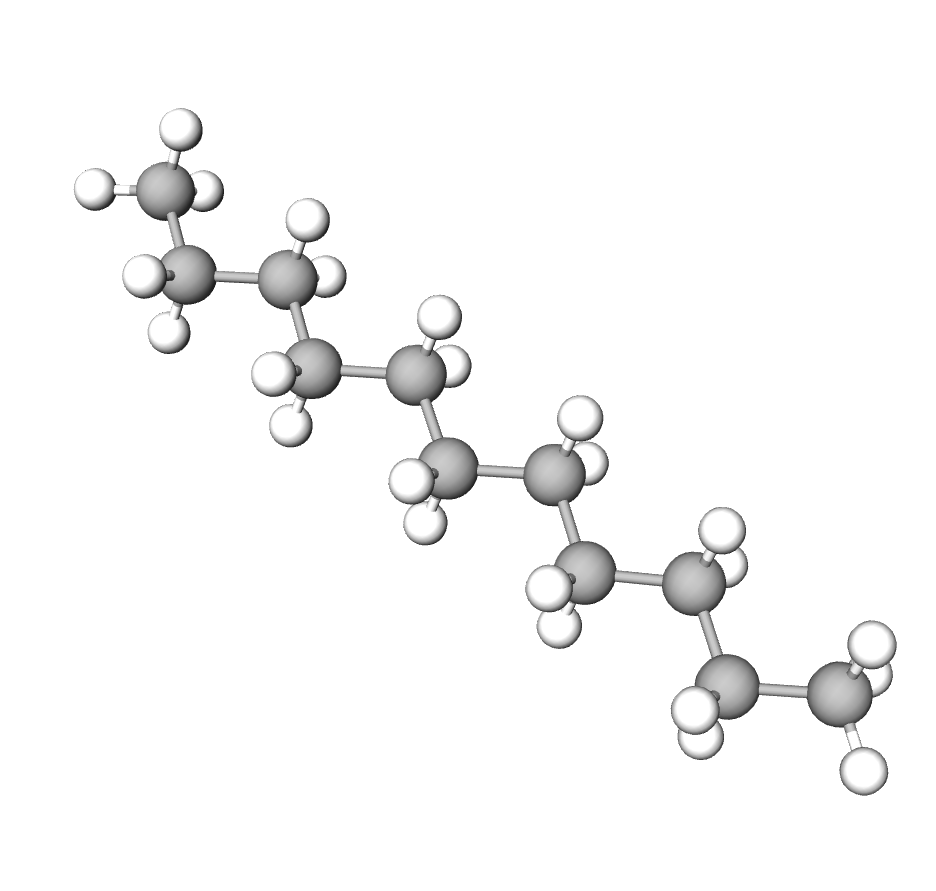
\includegraphics[]{polyethelene.png}
    \caption{Long chain molecule of polyethylene, a common material.}
\end{marginfigure} weakly held together by inter-molecular forces. Initially the molecules are likely to be tangled-up together. As force is applied it is initially difficult to move the polymer chains from this state (\textbf{A}). As the chains begin to unravel they straighten out by bond rotation, requiring relatively little force for a large increase in strain (\textbf{B}). As the polymer chains become straight it becomes much more difficult to extend the material any further without damaging the material (\textbf{C}).

\begin{figure}[ht]
    \begin{center}
        \begin{tikzpicture}[scale=.75]
            \draw[thick, ->] (-0.5,0) -- (11,0) node[anchor=north] {$\epsilon$};
            \draw[thick, ->] (0,-0.5) -- (0,9) node[anchor=east] {$\sigma$};
            \draw (0,0) .. controls (3,7) and (6,1) .. (10,8);
            \draw (1.5,1) node{\textbf{A}};
            \draw (5,1) node{\textbf{B}};
            \draw (8.5,1) node{\textbf{C}};
            \draw[dashed] (3,0) -- (3,3.6);
            \draw[dashed] (7.2,0) -- (7.2,4.7);
        \end{tikzpicture}
    \end{center}
    \caption{Stress-strain curve for a polymer}
    \label{stress-strain-polymer}
\end{figure}

\section{Rubber}
When a rubber is exposed to stress or strain energy, internal rearrangements such as rotation and extension of the polymer chains occur. 
\begin{marginfigure}
    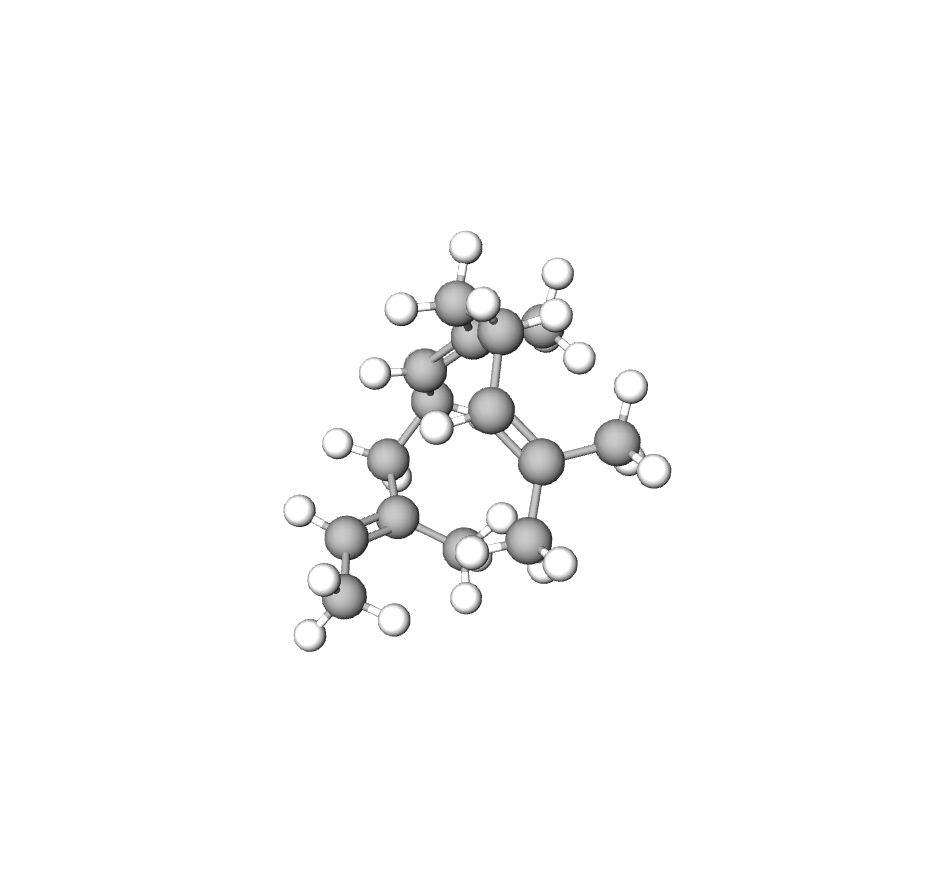
\includegraphics[]{figures/naturalrubber.png}
    \caption{The twisted structure of natural rubber}
\end{marginfigure} These changes occur as a function of the energy applied and the duration and rate of application, as well as the temperature at which the energy is applied.
The difference between the two curves is the hysteresis losses.
\begin{figure}
	\vspace*{-10pt}
	\centering
	\begin{tikzpicture}[scale=0.54]
	\draw[<->] (6.4,0) node[below]{strain} -- (0,0) -- (0,6.4) node[left]{stress};
	\draw[thick,blue,postaction={decorate},decoration={markings,mark=at position 0.5 with {\arrow{>}}}] (0,0) [out=60,in=210] to (3,4) [out=30,in=225] to (6,6);
	\draw[thick,blue,postaction={decorate},decoration={markings,mark=at position 0.5 with {\arrow{>}}}] (6,6) [out=240,in=30] to (3,3) [out=210,in=50] to (0,0);
	\end{tikzpicture}
	\vspace*{-16pt}
\end{figure}
	
\section{End-of-chapter questions}

\subsection*{Springs \& Hooke's law}

\begin{marginfigure}
	\vspace*{-5pt}
	\centering
	\begin{tikzpicture}
	\draw[help lines, gray!50, very thin, step=0.1] (0,0) grid (5,4);
	\draw[help lines, step=1] (0,0) grid (5,4);
	\foreach \y in {0,1,2,3, 4} \node[left] at (0,\y) {$\y$};
	\foreach \x in {0,1,2,3,4,5} \node[below] at (\x,0) {$\x$};
	\node at (-1,3.5) {load/kg};
	\node at (4,-0.8) {extension/cm};
	\draw[thick,blue] (0,0) -- (5,3.2);
	\end{tikzpicture}
	\vspace*{-25pt}
\end{marginfigure}

\subsection*{Stress, Strain, \& Young modulus}

\begin{marginfigure}
	\vspace*{5pt}
	\centering
	\begin{tikzpicture}
	\draw[help lines, gray!50, very thin, step=0.1] (0,0) grid (5,5);
	\draw[help lines, step=1] (0,0) grid (5,5);
	\foreach \y in {0,1,2,3,4,5} \node[left] at (0,\y) {$\y$};
	\foreach \x in {0,0.1,0.2,0.3,0.4,0.5} \node[below] at (10*\x,0) {$\x$};
	\node at (-1,4.5) {$F$/N};
	\node at (4,-0.8) {$x$/mm};
	\draw[thick,blue] (0,0) -- (5,2.4);
	\end{tikzpicture}
	\vspace*{-25pt}
\end{marginfigure}

\begin{marginfigure}
	\vspace*{-10pt}
	\centering
	\begin{tikzpicture}[scale=0.54]
	\draw[<->] (6.4,0) node[below]{strain} -- (0,0) -- (0,6.4) node[left]{stress};
	\draw[thick,blue,postaction={decorate},decoration={markings,mark=at position 0.5 with {\arrow{>}}}] (0,0) [out=60,in=210] to (3,4) [out=30,in=225] to (6,6);
	\draw[thick,blue,postaction={decorate},decoration={markings,mark=at position 0.5 with {\arrow{>}}}] (6,6) [out=240,in=30] to (3,3) [out=210,in=50] to (0,0);
	\end{tikzpicture}
	\vspace*{-16pt}
\end{marginfigure}

\cleardoublepage

% ===== Chapter: waves =====
\chapter{Waves}

A wave is a way of transferring and storing \emph{energy} without the transport of matter. Most familiar examples are surface waves on water, sound waves, light waves. In the next two chapters, we are going to look at the basics of wave motion and some of the most important wave phenomena.

Wave motion is the propagation of disturbance -- deviations from a state of equilibrium -- from one place to another. 

% Waves consist of continuous oscillations around some fixed locations.

% There are mainly two types of waves, \keypoint{mechanical waves} and \keypoint{electromagnetic waves}. Mechanical waves propagate as oscillations of matter, thus it must travel through a \emph{medium}. Electromagnetic waves can travel in free space.

% A wave can either be \keypoint{transverse} or \keypoint{longitudinal} depending on the direction of its oscillation. The direction of propagation of a transverse wave is perpendicular to the direction of its oscillation, and the wave motion of a longitudinal wave is parallel to its oscillation.

\subsection{Wave terminology}

Wave motion is the propagation of disturbance from one place to another

\begin{figure*}[ht]
	\centering
	\begin{tikzpicture}[xscale=1.2, yscale=0.95]
	\draw [->] (0,-2) -- (0,2.4) node[midway,left]{$O$} node[above]{displacement};
	\draw [->] (0,0) -- (3.1*pi,0) node[below]{position};
	\draw[very thick,->] (1.8*pi,2) -- (2.6*pi,2);
	\node[above,twoline] at (2.2*pi, 2.1) {direction of\\wave motion};
	\foreach \t/\labelcolor in {1/{blue}, 2/{Green}, 3/{purple}, 4/{gray}} {
		\draw[\labelcolor] ({0.4*pi+(\t-1)*0.6)}, 1.7) --++ (0.2,0.5) node[above]{$t_\t$};
		\draw [thick, \labelcolor, domain=0:3*pi, samples=30, smooth] plot (\x,{1.6*sin((\x+0.6-0.6*\t)*1.25 r)});
	}
	\end{tikzpicture}
	
	\caption{wave pattern at different times ($t_1<t_2<t_3<t_4$) as wave travels in space}
\end{figure*}

To describe the wave motion and particle vibrations, we can define the following quantities:

\titem as a wave moves from the source, each point oscillates back and forth about their rest positions. The distance from a particle's equilibrium position is called \keypoint{displacement} of the particle \index{displacement}. The greatest displacement for a particle is called the \keypoint{amplitude} ($A$) \index{amplitude}.

A wave pattern repeats itself over a certain distance, the distance between two adjacent points undergoing exactly same motion is the \keypoint{wavelength} ($\lambda$) \index{wavelength}. One can think of wavelength as crest-to-crest distance, trough-to-trough distance, etc.\footnote{For now, we take for granted that a wave is transverse. There are also longitudinal waves for which terms like crest and trough do not apply. We will get into that in \S\ref{ch-Lwaves}.}

You can also think about how each point also repeats its vibrational motion over a certain time interval. The time for a particle to complete a full oscillation cycle is the  \keypoint{period} ($T$) \index{period}. The number of oscillations for a particle per unit time is the \keypoint{frequency} ($f$) \index{frequency} which can also be defined as the number of crests passing a given point per unit time.\\

The frequency of a wave is related to its period by \begin{empheq}[box=\tcbhighmath]{equation*}{f=\frac{1}{T}}\end{empheq}

The unit of frequency: $[f] = \text{Hz}$ (hertz), where $1 \text{ Hz} = 1 \text{ s}^{-1}$. There's some useful coded language here, many things are ``per second'', the ``Hertz'' part tell you it's probably a wave you're talking about.

\begin{figure*}[ht]
	\centering
	\begin{minipage}{0.48\textwidth}
		\centering
		\begin{tikzpicture}[scale=0.55]
		\draw [->] (0,-2) -- (0,2) node[midway,left]{$O$} node[above]{displacement};
		\draw [->] (0,0) -- (3*pi,0) node[below]{position};
		\draw [very thick,blue,domain=0:3*pi,samples=30,smooth,variable=\x] plot (\x,{1.6*sin(\x*1.25 r)});
		\draw[<->, thick, red] (.4*pi,1.6) -- (.4*pi,0) node[midway,right]{$A$};
		\draw[<->, thick, red] (.4*pi,1.8) -- (2*pi,1.8) node[midway,above]{$\lambda$};
		\end{tikzpicture}
		
		wave pattern of all particles at one instant
	\end{minipage}\hfil
	\begin{minipage}{0.48\textwidth}
		\centering
		\begin{tikzpicture}[scale=0.55]
		\draw [->] (0,-2) -- (0,2) node[midway,left]{$O$} node[above]{displacement};
		\draw [->] (0,0) -- (3*pi,0) node[below]{time};
		\draw [very thick,blue,domain=0:3*pi,samples=30,smooth,variable=\x] plot (\x,{1.6*sin(\x*1.25 r)});
		\draw[<->, thick, red] (.4*pi,1.6) -- (.4*pi,0) node[midway,right]{$A$};
		\draw[<->, thick, red] (.4*pi,1.8) -- (2*pi,1.8) node[midway,above]{$T$};
		\end{tikzpicture}
		
		vibration of one specific particle at all times
	\end{minipage}
\end{figure*}

Wave energy is transferred along the direction of wave motion at a certain speed $v$. In one period, the wave moves forward by a distance of one wavelength, so \keypoint{wave speed} \begin{empheq}[box=\tcbhighmath]{equation*}{v=\frac{\lambda}{T}}\end{empheq}, or in terms of frequency, \begin{empheq}[box=\tcbhighmath]{equation*}{v=\lambda f}\end{empheq}

\subsection{Transverse \& longitudinal waves}

A wave can either be \emph{transverse} or \emph{longitudinal}, depending on the direction of its oscillation

\subsection{Transverse waves}

\begin{ilight}
	\centering A \keypoint{transverse} wave has vibrations at right angle to its direction of energy transfer \index{transverse wave}.
\end{ilight}

Examples of transverse waves: 
\titem wave on a string, 
\titem surface wave on water, 
\titem light wave, etc.

For a transverse wave, greatest displacement in positive direction is called a \emph{crest}, or a \emph{peak}, the greatest displacement in negative direction is called a \emph{trough}.

\subsection{Longitudinal waves} \label{ch-Lwaves}

\begin{ilight}
	\centering A \keypoint{longitudinal} wave has vibrations in parallel direction to energy transfer \index{longitudinal wave}.
\end{ilight}

Examples of longitudinal waves: 
\titem sound waves, 
\titem wave along a stretched slinky, etc.

For a longitudinal wave, if medium gets squeezed, we say this region is a \emph{compression}, if a medium expands, we say this region is a \emph{rarefaction}.  The wavelength of a longitudinal wave can be defined as compression-to-compression distance.

\begin{figure*}[ht]
	\centering
	\begin{tikzpicture}[xscale=1, yscale=1.7]
	\foreach \x in {-0.75,-0.5,...,10.75}
	\draw[thick] ({\x} , -1) --++ (0,1);
	\end{tikzpicture}
	
	All particles at their equilibrium position before a pressure wave is set up
\end{figure*}

\begin{figure*}[ht]
	\centering
	\begin{tikzpicture}[xscale=1, yscale=1.7]
	\foreach \x in {-0.75,-0.5,...,11} 
		\draw[thick] ({\x+0.5*cos(\x*0.5*pi r)} , -1) --++ (0,1);
	\foreach \x in {-0.5,-0.25,...,11.25} 
		\draw[thick] ({\x+0.5*cos((\x-1)*0.5*pi r)} , -2.5) --++ (0,1);
	\foreach \x in {-0.5,-0.25,...,11} 
		\draw[thick] ({\x+0.5*cos((\x-2)*0.5*pi r)} , -4) --++ (0,1);
		\foreach \x in {3,7} \node[Green] at (\x,-1.2) {\phantom{p}rarefaction\phantom{p}};
		\foreach \x in {1,5,9} \node[blue] at (\x,-1.2) {compression};
		\foreach \x in {0,4,8} \node[Green] at (\x,-2.7) {\phantom{p}rarefaction\phantom{p}};
		\foreach \x in {2,6,10} \node[blue] at (\x,-2.7) {compression};
		\foreach \x in {1,5,9} \node[Green] at (\x,-4.2) {\phantom{p}rarefaction\phantom{p}};
		\foreach \x in {3,7} \node[blue] at (\x,-4.2) {compression};
		\node at (-1.5,-0.5) {{\large $t_1$}};
		\node at (-1.5,-2) {{\large $t_2$}};
		\node at (-1.5,-3.5) {{\large $t_3$}};
		\draw[very thick,->] (2.8,0.3) -- (7.2,0.3);
		\node[above,twoline] at (5, 0.4) {direction of wave motion};
		\draw[thick,red,<->] (1,-0.5) -- (5,-0.5) node[above,pos=0.55]{$\lambda$};
	\end{tikzpicture}
	
	\caption{compression and rarefaction regions at different times ($t_1<t_2<t_3$)	as a longitudinal pressure wave travels in space}
\end{figure*}

\subsection{Sound waves}

Sound waves propagate via the compression and rarefaction of air (or other medium) \index{Sound}

Molecules near vibrating source is pushed away from rest positions and into their neighbours, which then in turn push into their neighbours, and so on. In this manner the disturbance is transferred through the medium, forming a sound wave. The sound waves are longitudinal.
	
\begin{figure*}[ht]

\begin{tikzpicture}[scale=1]
\pgfmathsetmacro{\noe}{6}

\foreach \t in {0,0.1,...,14}{
	\pgfmathsetmacro{\np}{pow({1+cos((\t-2)*pi/2.5 r)}, 4)*\noe/4}
	\foreach \idx in {0,1,...,\np} {
		\draw[fill] (\t+rnd*0.1-0.05,rnd*1.8) circle (0.025);	% wave 1
	}
}
\draw[<->,thick] (7,2.4) -- (12,2.4) node[midway,above]{{\footnotesize one wavelength}};
\draw[->,thick] (1,2.4) -- (4,2.4) node[midway,above]{{\footnotesize wave motion}};
\node[below] at (2,-.2) {{\footnotesize compression}};
\node[below] at (7,-.2) {{\footnotesize compression}};
\node[below] at (12,-.2) {{\footnotesize compression}};
\node[below] at (4.5,-.2) {{\footnotesize rarefaction}};
\node[below] at (9.5,-.2) {{\footnotesize rarefaction}};
\end{tikzpicture}
\end{figure*}

Propagation of sound waves require medium (air, water, steel, etc.) which means that sound cannot travel in vacuum. The speed of sound is material-dependent, but not frequency-dependent, for example, sound in general travels faster in denser medium.
	
	\titem $v_\text{air} \approx 340 \mps$ (under standard atmospheric pressure and room temperature)
	
	\titem $v_\text{water} \approx 1500 \mps$
	
	\titem $v_\text{steel} \approx 5000 \mps$
	
The \emph{pitch} of a note is related to frequency of sound wave, rapid vibrations of sound source at high frequencies produce a high pitch. The \emph{loudness} of sound mainly depends on amplitude of vibration. A greater amplitude means the wave is more energetic so it sounds louder.
	
\subsection*{Measurement of sound waves}

Two key apparatuses for sound measurement are the \keypoint{microphone} and the \keypoint{oscilloscope}. \index{oscilloscope}
Sound waves can be captured by a \emph{microphone}, which converts sound into electrical signals, electrical signals can then be sent into an \emph{oscilloscope} (see figure\footnote{The beautiful figure of the oscilloscope was created by \emph{Hugues Vermeiren}, who generously shared the source codes on TeXample: \url{http://www.texample.net/tikz/examples/textronics-oscilloscope/}}) for measurement. The oscilloscope can be thought as an upgraded voltmeter that shows how voltage varies with time.

\begin{figure}[ht]
	\centering
	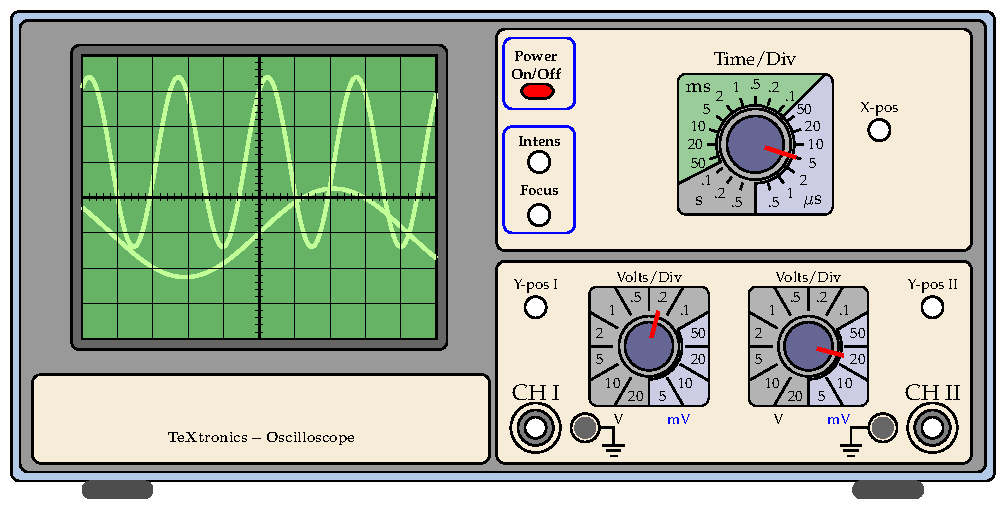
\includegraphics{oscilloscope.pdf}
	\caption{the display and controls of a typical cathode-ray oscilloscope}
\end{figure}

Oscilloscopes displays the variation of voltage ($y$-axis) with time ($x$-axis). The horizontal scale (time axis) is given by \emph{time-base} settings, the vertical scale (voltage axis) is given by \emph{voltage gain}, or \emph{Y-sensitivity} settings. The period $T$ of the sound wave can be found using time-base settings and the frequency calculated by: $f=\frac{1}{T}$. The voltage amplitude can be found using the voltage gain.

\begin{marginfigure}
	\vspace*{-12pt}
	\centering
	\begin{tikzpicture}[scale=0.8]
	\draw[fill=gray!80, rounded corners] (-0.2,-3.2) rectangle (7.2,3.2);
	\draw[Green!50, fill] (0,-3) rectangle (7,3);
	\draw[Green!20, ultra thick, domain=0:7, samples=100] plot (\x, {2*sin((\x-0.6)*120)});
	\draw[black!80, step=1] (0,-3) grid (7,3);
	\end{tikzpicture}
	\vspace*{-16pt}
\end{marginfigure}

\subsection{Electromagnetic waves}

A wave can be either \emph{mechanical} or \emph{electromagnetic}, depending on whether it requires a medium\index{electromagnetic wave}. Waves that require a \emph{medium} to travel are called \keypoint{mechanical waves}, examples are sound waves, water waves, wave on a string, etc.

Mechanical waves on the other hand, involve vibration of matter particles. No medium is needed for propagation of \keypoint{electromagnetic waves} i.e., they can travel in vacuum.

\subsection{Properties of electromagnetic waves}

\titem electromagnetic waves can travel in free space

\titem electromagnetic waves involve vibrations of electric and magnetic fields -- an altering electric field can generate an altering magnetic field, which then further produces a new altering electric field, so on and so forth. Electric and magnetic fields then permeate through space, transferring energy and information.
	
\titem electromagnetic waves are all transverse.
	
\titem vibration of electric fields and magnetic fields are both perpendicular to wave motion.

\begin{figure*}[ht]
	\centering
	\begin{tikzpicture}[xscale=0.72]
	\draw[Green, thick, ->] (0,-2.1) -- (0,2.1) node[left, twoline] {electric\\field};
	\draw[blue, thick, dotted] (0 ,0) -- (0.7, 1.4);
	\draw[blue, thick, ->] (0, 0) -- (-0.7,-1.4) node[left, twolinecap] {magnetic\\field};
	\draw[thick, ->] (-0.3,0) -- (14,0) node[right, twoline]{direction\\ of energy\\transfer};
	\draw[Green, thick, domain=0:13.5, samples=150] plot (\x, {1.6*sin(2*\x r)});
	\draw[blue, thick] plot [smooth] coordinates {
		(0, 0)
		(0.0007, -0.1987)
		(0.0053, -0.3894)
		(0.0177, -0.5646)
		(0.0413, -0.7174)
		(0.0793, -0.8415)
		(0.134, -0.932)
		(0.2073, -0.9854)
		(0.3002, -0.9996)
		(0.4131, -0.9738)
		(0.5454, -0.9093)
		(0.6958, -0.8085)
		(0.8623, -0.6755)
		(1.0422, -0.5155)
		(1.2325, -0.335)
		(1.4294, -0.1411)
		(1.6292, 0.0584)
		(1.8278, 0.2555)
		(2.0213, 0.4425)
		(2.2059, 0.6119)
		(2.3784, 0.7568)
		(2.5358, 0.8716)
		(2.6758, 0.9516)
		(2.7968, 0.9937)
		(2.8981, 0.9962)
		(2.9795, 0.9589)
		(3.0417, 0.8835)
		(3.0864, 0.7728)
		(3.1156, 0.6313)
		(3.1323, 0.4646)
		(3.1397, 0.2794)
		(3.1415, 0.0831)
		(3.1417, -0.1165)
		(3.1442, -0.3115)
		(3.1529, -0.4941)
		(3.1715, -0.657)
		(3.2032, -0.7937)
		(3.2506, -0.8987)
		(3.316, -0.9679)
		(3.4007, -0.9985)
		(3.5053, -0.9894)
		(3.6296, -0.9407)
		(3.7727, -0.8546)
		(3.9328, -0.7344)
		(4.1075, -0.5849)
		(4.2939, -0.4121)
		(4.4886, -0.2229)
		(4.6876, -0.0248)
		(4.8872, 0.1743)
		(5.0832, 0.3665)
		(5.272, 0.544)
		(5.4499, 0.6999)
		(5.6139, 0.8278)
		(5.7614, 0.9228)
		(5.8905, 0.9809)
		(6, 1)
		(6.0896, 0.9792)
		(6.1597, 0.9193)
		(6.2114, 0.8228)
		(6.2468, 0.6935)
		(6.2683, 0.5366)
		(6.2791, 0.3582)
		(6.2828, 0.1656)
		(6.2832, -0.0336)
		(6.2842, -0.2315)
		(6.2899, -0.4202)
		(6.304, -0.5921)
		(6.3298, -0.7404)
		(6.3704, -0.8592)
		(6.4282, -0.9437)
		(6.5047, -0.9906)
		(6.601, -0.998)
		(6.7172, -0.9657)
		(6.8526, -0.8948)
		(7.0059, -0.7883)
		(7.1749, -0.6503)
		(7.3568, -0.4864)
		(7.5484, -0.3031)
		(7.7461, -0.1078)
		(7.946, 0.0919)
		(8.144, 0.2879)
		(8.3362, 0.4724)
		(8.5191, 0.6381)
		(8.6892, 0.7784)
		(8.8438, 0.8876)
		(8.9807, 0.9614)
		(9.0985, 0.9969)
		(9.1963, 0.9927)
		(9.2744, 0.9488)
		(9.3336, 0.8672)
		(9.3755, 0.751)
		(9.4024, 0.6048)
		(9.4173, 0.4346)
		(9.4235, 0.247)
		(9.4248, 0.0495)
		(9.4251, -0.1499)
		(9.4283, -0.3433)
		(9.4385, -0.5231)
		(9.459, -0.682)
		(9.4932, -0.8137)
		(9.5435, -0.9129)
		(9.6121, -0.9758)
		(9.7001, -0.9998)
		(9.808, -0.9839)
		(9.9356, -0.9288)
		(10.0817, -0.8367)
		(10.2444, -0.7112)
		(10.4213, -0.5573)
		(10.6094, -0.3813)
		(10.805, -0.19)
		(11.0044, 0.0089)
		(11.2037, 0.2073)
		(11.3988, 0.3976)
		(11.586, 0.5719)
		(11.7617, 0.7235)
		(11.9231, 0.8462)
		(12.0676, 0.9352)
		(12.1935, 0.9869)
		(12.2996, 0.9993)
		(12.3859, 0.9718)
		(12.4528, 0.9056)
		(12.5016, 0.8033)
		(12.5345, 0.6689)
		(12.5539, 0.5079)
		(12.5633, 0.3266)
		(12.5662, 0.1324)
		(12.5664, -0.0672)
		(12.568, -0.2641)
		(12.5748, -0.4504)
		(12.5906, -0.6188)
		(12.6187, -0.7626)
		(12.6621, -0.8759)
		(12.7229, -0.9543)
		(12.8027, -0.9946)
		(12.9023, -0.9954)
		(13.0218, -0.9564)
		};
	\end{tikzpicture}
	\caption{variation in electric and magnetic fields for an electromagnetic wave}
\end{figure*}

Note that all electromagnetic waves travel at a constant speed $c=3.0\times10^8\mps$ in free space i.e., speed of light in vacuum is constant\footnote{The speed of light in vacuum is actually a \emph{universal} physical constant. According to Einstein's special relativity, this is the upper limit for the speed at which matter and information can travel. This speed is also independent of the inertial reference frame one chooses, i.e., the speed of light in vacuum is the same for all observers, regardless of the motion of the source or the observer.}

\newpage
\subsection{The electromagnetic spectrum}

Electromagnetic waves come in a wide range of wavelengths and frequencies, the distribution of electromagnetic radiation according to wavelength or frequency is the \keypoint{electromagnetic spectrum}\index{electromagnetic spectrum} (see diagram)

\begin{figure*}[!ht]
	\centering
	\begin{tikzpicture}[yscale=1.04]
	% define visible spectrum shading
	\pgfdeclareverticalshading{visible}{100bp}
	{color(0bp)=(violet!70); color(25bp)=(violet!70); color(35bp)=(blue!70);
		color(45bp)=(green!70); color(55bp)=(yellow!70); color(65bp)=(orange);
		color(75bp)=(red); color(100bp)=(red)}
	% grayish background for spectrum labels
	\draw[gray!15,fill] (-1.5,-8) rectangle (1.5,7.5);
	% axes
	\draw (-1.5,-8) -- (-1.5,7.5) (1.5,-8) -- (1.5,7.5);
	\node at (-3,7.7) {wavelength};
	\node at (3,7.7) {frequency};
	% spectrum labels
	\shade[shading=visible] (-1.5,-1.15) rectangle (1.5,-0.75);
	\foreach \x/\xlabel in {1.8/{radio waves}, -2/{microwaves}, -4.6/{infrared}, -6.35/{visible light}, -7.8/{ultraviolet}, -11/{X-rays}, -14.8/{$\gamma$-rays} } \node at (0,{\x*0.7+3.5}) {\xlabel};
	% values of wavelengths
	\foreach \x in {5,3,1,...,-15} {
		\draw (-1.5,{\x*0.7+3.5}) --++ (-0.5,0);
		\node at (-3,{\x*0.7+3.5}) {$10^{\x}$ m};
	}
	% values of frequencies
	\foreach \x in {3,5,...,23} {
		\draw (1.5,{-\x*0.7+8.8}) --++ (0.5,0);
		\node at (3,{-\x*0.7+8.8}) {$10^{\x}$ Hz};
	}
	% dashed lines as separators
	\foreach \x in {-1,-3,-9,-13} \draw[dashed,thick] (-1.5,{\x*0.7+3.5}) --++ (3,0);
	% extension for visible spectrum
	\draw[thick, gray!75] (1.5,-1.15) --++ (3,0) -- (5,-3);
	\draw[thick, gray!75] (1.5,-0.75) --++ (3,0) -- (5,1);
	\shade[shading=visible] (5,-3) rectangle (7,1);
	\node at (6, 1.3) {visible light};
	\node[right] at (7.2, 0.8) {700 nm};
	\node[right] at (7.2, -2.8) {400 nm};
	\end{tikzpicture}
	\caption{the electromagnetic spectrum}
\end{figure*}

\newpage

The table below shows electromagnetic spectrum in somewhat more precise details \footnote[][-2cm]{There are no precise accepted boundaries between different ranges in the electromagnetic spectrum. The boundaries are actually somewhat ambiguous. The ranges of different portions tend to overlap. For example, a large portion of the ranges of X-rays overlap with that of $\gamma$-rays, and microwaves are considered by many people as a subdivision of radio waves. Therefore, the values given here are merely supposed to give you some rough idea about the order of magnitudes for electromagnetic wavelengths and frequencies. So the point I want to make here is: do not take the borderlines too seriously.}
\vspace{3cm}
\begin{figure*}
\begin{center}
	\begin{tabular}{|C{4cm}|C{4cm}|C{4cm}|}
		\hline Region of spectrum & Range of wavelength & Range of frequency \\ 
		\hline radio waves  & 10$^{-1}$ $\sim$ 10$^{6}$ m & 10$^{2}$ $\sim$ 10$^{9}$ Hz \\ 
		\hline microwaves & 10$^{-3}$ $\sim$ 10$^{-1}$ m & 10$^{9}$ $\sim$ 10$^{11}$ Hz \\ 
		\hline infra-red & 7$\times$10$^{-7}$ $\sim$ 10$^{-3}$ m & 10$^{11}$ $\sim$ 10$^{14}$ Hz \\ 
		\hline visible light  & 4$\times$10$^{-7}$ $\sim$ 7$\times$10$^{-7}$ m & 10$^{14}$ $\sim$ 10$^{15}$ Hz \\ 
		\hline ultraviolet & 10$^{-9}$ $\sim$ 4$\times$10$^{-7}$ m & 10$^{15}$ $\sim$ 10$^{17}$ Hz \\ 
		\hline X-rays & 10$^{-13}$ $\sim$ 10$^{-9}$ m & 10$^{17}$ $\sim$ 10$^{19}$ Hz \\ 
		\hline $\gamma$-rays & 10$^{-16}$ $\sim$ 10$^{-11}$ m & 10$^{19}$ $\sim$ 10$^{24}$ Hz\\ 
		\hline
	\end{tabular} 
\end{center}
\end{figure*}

Each type of electromagnetic waves has important applications in some area
\footnote{The entries listed here only include a teeny-weeny part of the uses of electromagnetic radiation, somewhat based on my personal taste. I also included a handful of explanations for the examples that I found interesting (otherwise I would not choose them), as you will see a huge load of footnotes in the next few pages. You are encouraged to do some researches as well, I can guarantee that you will not be disappointed.}

\begin{compactitem}
	\item[--] Radio waves.
	
	\xskip Telecommunication (TV/radio broadcast, satellite communication). Having the longest wavelengths of all radiation, radio waves have the best ability to diffract around obstacles in city buildings and mountains, therefore a large area can be covered.

	\item[--] Microwaves.
	
	\xskip Telecommunication (mobile phones, WiFi, Bluetooth, satellite communication). Microwaves do not diffract sufficiently as radio waves, but they can transmit more information per unit time because they have higher frequencies. Microwaves are used in short-range telecommunication, including mobile phones, wireless networks, and bluetooth connections.
		
		
	\xskip Heating food (microwave ovens). Frequency of microwaves are close to the natural frequencies of the rotational motion of water molecules. When food is exposed to microwaves, the water molecules in the food resonate and vibrate more violently, causing a rise in the food's temperature.
	
	\item[--] Infrared (IR).
	
	\xskip IR thermography (temperature monitors, thermographic cameras). All objects emit electromagnetic radiation based on their temperatures. According to the law of black-body radiation, objects near room temperature emit thermal energy as infrared radiation, so variations in the temperature can be detected.
	
	\xskip Night-vision devices. Night-vision devices convert photons (just think of them as particles of light for now) into electrons, which are amplified by a chemical and electrical process and then converted back into visible light. Infrared sources can be used to augment the available light, increasing the visibility in the dark.
	
	\xskip IR heating (IR heat lamps, IR saunas). 	
	\xskip IR data transmission (remote controls, optical-fibre communication)	
	\item[--] Visible Light
	
	\xskip Human Vision. Human eyes are only sensitive to a small fraction of the electromagnetic spectrum. The wide variety of colours that we see is actually built up from the relative intensities of red, green and blue light collected by the three colour detectors in our eyes.
	
	\item[--] Ultraviolet (UV).
	
	\xskip UV sterilising (drinking water treatment, disinfection of medical facilities, etc.) Short-wavelength UV light can damage the DNA's in living organisms. A microorganism exposed to germicidal UV light might not be able to reproduce, and becomes harmless. For the same reason, overexposure to UV radiation present in the sunlight can cause sunburn, or even skin cancer.
		
	\xskip Fluorescent dyes (black light fluorescent paint, UV watermarks) UV radiation can cause many substances to glow through chemical reactions. UV watermarks that are visible under UV light are used to prevent counterfeiting of currency, or forgery of important documents such as passports and ID cards.
	
	\item[--] X-rays.
	
	\xskip Medical imaging (X-ray imaging, CT scans). X-rays are very energetic and thus very penetrating. They can pass through human body easily to form an image giving information about the structures of tissues and bones.
	
	\xskip Security checking (luggage scanners).
	
	\xskip X-ray crystallography. X-rays can be diffracted by the lattice of atoms in a crystal. The diffraction pattern gives information about the structure of the lattice. X-ray crystallography is a very important experimental technique to study the microscopic structures of new materials.
	
	\item[--] $\gamma$-rays.
	
	\xskip Radiation therapies (cancer treatment). $\gamma$-rays have extremely high frequencies. They are even more energetic and penetrating. They can be used to damage the DNA of cancerous tissue, and hence kill the cancerous cells as a treatment.
	
	\xskip Medical imaging (PET scans). Positron emission tomography (PET) uses a radioactive tracer to produce $\gamma$-rays within the tissues of interest. The energy and location of these $\gamma$-rays can be detected and sent to a computer to build up a 3D image of the body part.
\end{compactitem}
\newpage

	

\subsection{Wave intensity}

Energy can be transmitted along a wave, the degree to which this energy is concentrated is called the intensity of the wave. In this case ``concentration'' has two meanings -- concentration in time and concentration in area $S$\footnote{To avoid confusion, I reserved letter `$A$' for wave amplitude and chose `$S$' to represent an area.}

\begin{ilight}
	\centering \keypoint{intensity} of a wave is defined as the power $P$ per unit area on a cross section $S$: \begin{empheq}[box=\tcbhighmath]{equation*}{I=\frac{P}{S}}\end{empheq}\index{wave intensity}
\end{ilight}

The unit of wave intensity is Watts per meter: $[I] = \text{ W m}^{-2}$

\sidenote[][]{\piste The intensity is proportional to square of its amplitude: $\boxed{I \propto A^2}$}.

The intensity of a wave decreases as it spreads out in space, in fact Intensity is a great example of the \emph{inverse square law}. Intensity at distance of $r$ from a point source is inversely proportional to $r^2$: $\tcbhighmath{I \propto \frac{1}{r^2}}$
\footnote{As a wave produced from a point source travels out by a distance $r$ away from the source, the energy it carries is spread uniformly over the surface area of the sphere of radius $r$, that is: $S=4\pi r^2$. So the intensity of a wave obeys an inverse square law: $I \propto \frac{1}{r^2}$.}

\subsection{Polarisation}

\subsection{Plane polarisation}

\begin{ilight}
	A wave is \keypoint{plane-polarised}, or simply \keypoint{polarised}, if the vibration is in one single direction at right angle to the direction of propagation of energy\index{polarisation}
\end{ilight}

\begin{figure}[ht]
	\centering
	\begin{minipage}{0.45\textwidth}
		\centering
		\begin{tikzpicture}[scale=0.64]
		\draw[very thick, blue, ->] (210:2) -- (30:8) node[twoline, above, black]{direction of\\energy transfer};
		\foreach \t in {0,45,90,135} {
			\draw[red, ultra thick, <->] (\t:1.5) --++ ({\t+180}:3);
			\draw[red, ultra thick, <->] (30:3.5) ++ (\t:1.5) --++ ({\t+180}:3);
		}
		\end{tikzpicture}
		
		an unpolarised wave
		
		(wave vibrations in multiple directions)
	\end{minipage}\hfil
	\begin{minipage}{0.45\textwidth}
		\centering
		\begin{tikzpicture}[scale=0.64]
		\draw[very thick, blue, ->] (210:2) -- (30:8) node[twoline, above, black]{direction of\\energy transfer};
		\foreach \t in {90} {
			\draw[red, ultra thick, <->] (\t:1.5) --++ ({\t+180}:3);
			\draw[red, ultra thick, <->] (30:3.5) ++ (\t:1.5) --++ ({\t+180}:3);
		}
		\end{tikzpicture}
		
		a plane-polarised wave
		
		(wave vibrations in one direction only)
	\end{minipage}
\end{figure}

Polarisation\footnote[][-10cm]{\piste Apart from plane polarisation where the vibrations are fixed in a single direction, there are also \emph{circular} or \emph{elliptical} polarisation, for which the direction of vibrations \emph{rotate} in a plane as the wave travels.} is a phenomenon associated with \emph{transverse} waves only. Longitudinal waves (such as sound waves) cannot be polarised because longitudinal vibrations are always parallel to direction of energy transfer.

One of the most important examples are polarisation of \emph{electromagnetic waves}. Sunlight, light emitted from incandescent bulbs etc is unpolarised because they are emitted randomly from their sources, so they contain all planes of polarisation. Lasers, diodes, microwave antennae and a few others produce polarised emissions. 
A few of the great many applications of polarisation are:

\begin{compactitem}
	\item[--] polarising sunglasses \& photography \sidenote[][-10cm]{When unpolarised light is reflected at the boundary of two media, the reflected beam would become partially polarised. Polarising sunglasses use this effect to reduce the sunlight reflected from shiny surfaces, such as a lake (for sightseeing tourists) or road surfaces (for drivers). For the same reason, photographers often place a polarising filter in front of the camera lens to darken skies and increase the contrast.}
	
	\item[--] polarised 3D films\footnote[][-6.5cm]{The eyeglasses worn by viewers contain a pair of polarising filters with mutually perpendicular axes. When two images are projected onto the same screen, each filter restricts the light reaching each eye by passing only one of the images that is polarised in the same direction. This creates an 3D illusion.}
	
	\item[--] liquid-crystal display (LCD) technology\footnote[][-4cm]{Liquid crystal arrays can be realigned by applying an electric field. This causes the axis of polarization to rotate, hence backlight may be allowed to pass or be blocked, forming dark patterns of the display.}
	
	\item[--] radio transmission and reception\footnote[][-2cm]{Since electric currents flow in certain directions only, so the radio waves and microwaves produced from aerials are intrinsically polarised. This means the reception of signals would be sensitive to a particular direction, but totally insensitive to the normal direction. This explains why altering the orientation of antennas could greatly enhance the quality of reception.}
\end{compactitem}

\subsection{Polarisers \& Malus's law}

A plane-polarised light can be produced from unpolarised light using a \keypoint{polariser}.

A polariser blocks vibrations in all planes except the plane of polarisation. This type of polariser, often called a \emph{linear absorptive polariser}, is basically a synthetic transparent plastic sheet made of certain crystals. The thin sheet contains long-chain organic molecules aligned parallel to each other. When an unpolarised light passes through the polariser, there is a strong absorption of the electric field parallel to the alignment of molecules, so vibration of the electric field is allowed to pass in one direction only.

The direction along which vibration is allowed to pass is called the axis of the polariser

\begin{figure*}[ht]
	\centering
	\begin{tikzpicture}[scale=0.65]
	\draw[very thick, blue, ->] (0,0) -- (10,0);	
	\draw[fill=cyan!30] (0,0) ++ (0,2) ++ (160:2) --++ (-20:4) --++ (0,-4) --++ (160:4) --++ (0,4);
	\foreach \t in {-1.5,-1,...,1.5} \draw[very thin, gray!80, decorate, decoration={snake, amplitude=0.6}] (0,0) ++ (0,\t) ++ (160:1.6) --++ (-20:3.2);
	\draw[thick, Green, dashed] (0,1.8) -- (0,-1.8);
	\draw[Green] (0.1,1.2) -- (1.6,3) node[black, right, twoline]{axis of\\transmission};
	\draw[gray!80] (-1.4,1.6) -- (-3,3) node[black, left, twoline]{direction of alignment\\of molecules};
	\draw[very thick, blue] (-10,0) -- (0,0);
	\foreach \t in {-20,40,90,125} {
		\draw[red, ultra thick, <->] (-4,0) ++ (\t:1.5) --++ ({\t+180}:3);
		\draw[red, ultra thick, <->] (-8,0) ++ (\t:1.5) --++ ({\t+180}:3);
	}
	\foreach \t in {4,8} \draw[red, ultra thick, <->] (\t,-1.5) --++ (0,3);
	\node at (-6,-3.2) {unpolarised light};
	\node at (6,-3.2) {plane-polarised light};
	\node at (0,-3.2) {polariser};
	\end{tikzpicture}
	
	\caption{unpolarised light goes through a polariser and becomes plane-polarised}
\end{figure*}

Polarised light can be sent through a second polarising filter (sometimes called an \emph{analyser})

\begin{figure*}[ht]
	\centering
	\begin{minipage}{0.45\textwidth}
		\centering
		\begin{tikzpicture}[scale=0.4]
		\draw[very thick, blue, ->] (3,0) -- (8.4,0);	
		\draw[fill=orange!30] (3,0) ++ (0,2) ++ (160:2) --++ (-20:4) --++ (0,-4) --++ (160:4) --++ (0,4);
		\foreach \t in {-1.5,-1,...,1.5} \draw[very thin, gray!80, decorate, decoration={snake, amplitude=0.6}] (3,0) ++ (0,1.5) ++ (160:\t) --++ (0,-3);	
		\draw[very thick, blue] (-3,0) -- (3,0);	
		\draw[fill=cyan!30] (-3,0) ++ (0,2) ++ (160:2) --++ (-20:4) --++ (0,-4) --++ (160:4) --++ (0,4);
		\foreach \t in {-1.5,-1,...,1.5} \draw[very thin, gray!80, decorate, decoration={snake, amplitude=0.6}] (-3,0) ++ (0,\t) ++ (160:1.6) --++ (-20:3.2);	
		\draw[very thick, blue] (-8.4,0) -- (-3,0);
		\foreach \t in {-20,40,90,125} {
			\draw[red, very thick, <->] (-6.5,0) ++ (\t:1.5) --++ ({\t+180}:3);
		}
		\foreach \t in {0} \draw[red, very thick, <->] (\t,-1.5) --++ (0,3);
		\node at (-3,-3.5) {polariser};
		\node at (3,-3.5) {analyser};
		\end{tikzpicture}
		
		no transmission of light if polariser and 
		
		analyser are aligned at right angles
	\end{minipage}\hfil
	\begin{minipage}{0.45\textwidth}
		\centering
		\begin{tikzpicture}[scale=0.4]
		\draw[very thick, blue, ->] (3,0) -- (8.4,0);	
		\draw[fill=orange!30] (3,0) ++ (0,2) ++ (160:2) --++ (-20:4) --++ (0,-4) --++ (160:4) --++ (0,4);
		\foreach \t in {-1.5,-1,...,1.5} \draw[very thin, gray!80, decorate, decoration={snake, amplitude=0.6}] (3,0) ++ (0,\t) ++ (160:1.6) --++ (-20:3.2);	
		\draw[very thick, blue] (-3,0) -- (3,0);	
		\draw[fill=cyan!30] (-3,0) ++ (0,2) ++ (160:2) --++ (-20:4) --++ (0,-4) --++ (160:4) --++ (0,4);
		\foreach \t in {-1.5,-1,...,1.5} \draw[very thin, gray!80, decorate, decoration={snake, amplitude=0.6}] (-3,0) ++ (0,\t) ++ (160:1.6) --++ (-20:3.2);	
		\draw[very thick, blue] (-8.4,0) -- (-3,0);
		\foreach \t in {-20,40,90,125} {
			\draw[red, very thick, <->] (-6.5,0) ++ (\t:1.5) --++ ({\t+180}:3);
		}
		\foreach \t in {0,6.5} \draw[red, very thick, <->] (\t,-1.5) --++ (0,3);
		\node at (-3,-3.5) {polariser};
		\node at (3,-3.5) {analyser};
		\end{tikzpicture}
		
		polarised light is unaffected if polariser
		
		and analyser are aligned in parallel
	\end{minipage}
\end{figure*}

If polarised light of initial intensity $I_0$ has an angle $\theta$ to the axis of analyser then \keypoint{Malus's law}\footnote{\piste This isn't actually on the spec but it's pretty critical so we often include it.}\index{Malus's law} states that transmitted intensity is given by: $$\tcbhighmath{I = I_0 \cos^2 \theta}$$

This is because only electric field parallel to axis of analyser is transmitted, so transmitted amplitude\footnote{This is actually the amplitude of the electric field strength.} satisfies: $A = A_0 \cos\theta$, where $A_0$ is the initial amplitude.

Recall that intensity is proportional to square of amplitude, so $I = I_0 \cos^2 \theta $

\subsection{Doppler effect}

\begin{ilight}
	Relative motion between wave source and the observer causes a change in observed frequency, this is known as the \keypoint{Doppler effect}\index{Doppler effect}
\end{ilight}

Any type of wave can exhibit Doppler effect - we are extremely familiar with the changes in pitch as a car drives toward, alongside, then away from us. When wave source moves towards observer, a higher frequency is observed and when wave source moves away from observer, a lower frequency is observed. We can see clearly the direction in which these ducklings are swimming thanks to the same physics:
\begin{figure}
    \centering
    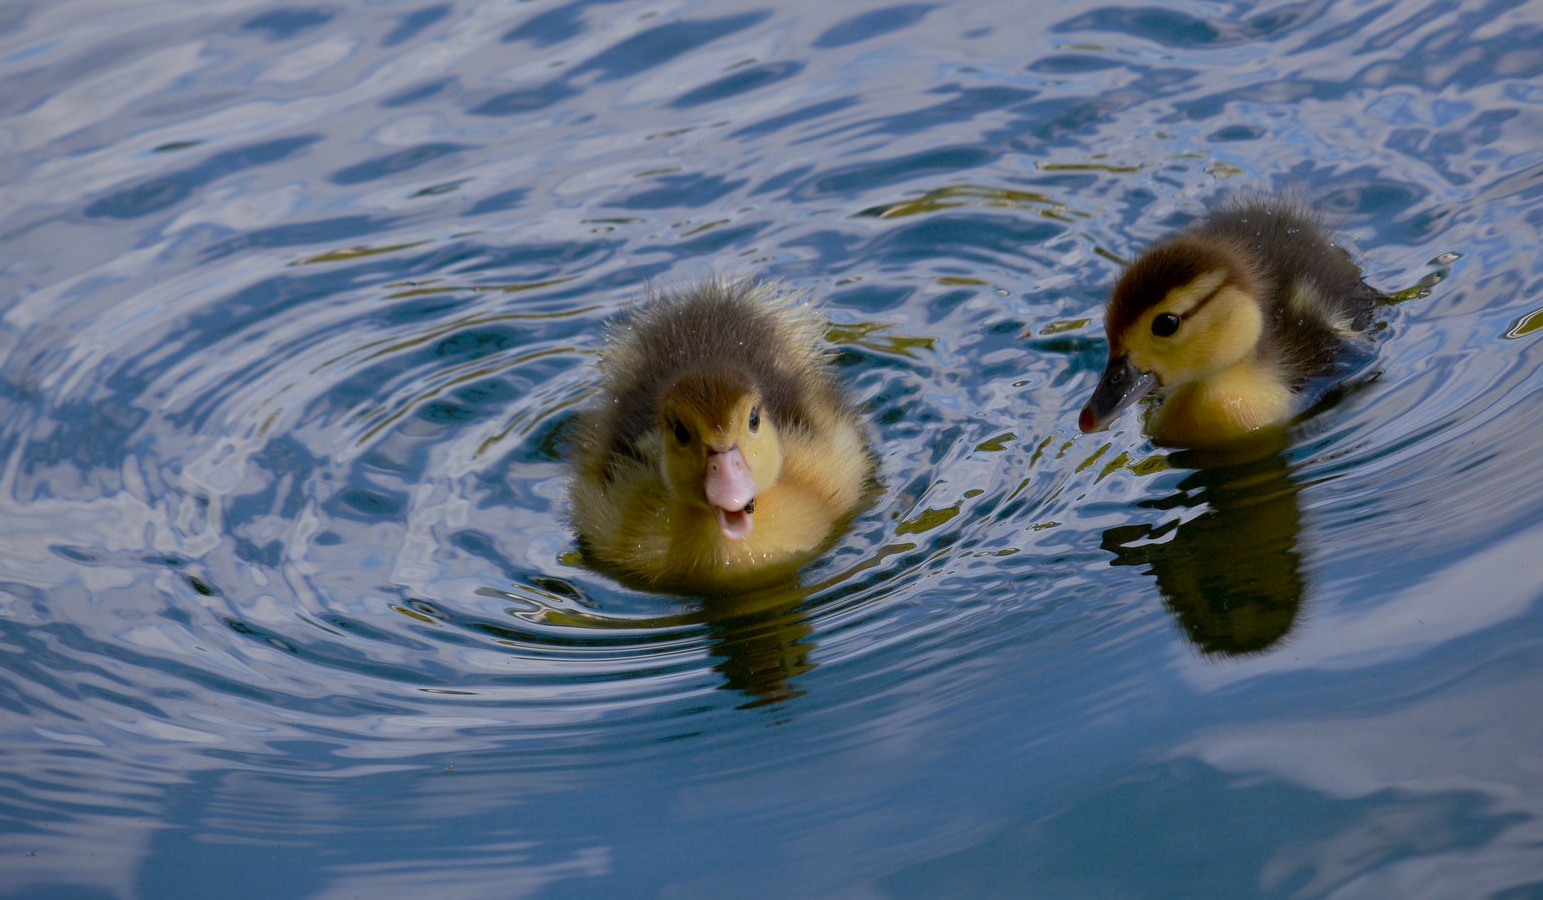
\includegraphics[width=0.75\linewidth]{figures/Swimduck.png}
    \caption{Doppler Ducks...}
    \label{fig:enter-label}
\end{figure}

The Doppler effect also occurs if source is at rest but observer is in motion, as long as there is \emph{radial} motion between source and observer, there is shift in frequency.

Doppler effect finds its use in many areas, some examples are

\begin{compactitem}
	\item[--] \emph{Doppler radars}: used to measure velocity of moving target (speeding cars, tennis balls, etc.)
	
	\item[--] \emph{Doppler ultrasonography}: used to image blood flow in human bodies
	
	\item[--] \emph{Astronomy}: used to study motion of stars and galaxies
\end{compactitem}

\newpage

\subsection*{Explanation of the Doppler effect}

Suppose wave source is moving towards the observer at speed $v_s$, at time $t=0$, the source emits a wavefront which travels at speed $v$.

\begin{figure*}[ht]
	\centering
	\begin{tikzpicture}[scale=0.95]
	\draw[thick] (0,0) circle (0.2);
	\draw[fill] (12,0.4) circle (0.2);
	\draw[ultra thick] (12,0.2) -- (12,-0.1) -- (11.8,-0.6) (12,-0.1) -- (12.2,-0.6) (11.75,-0.1) -- (12,0.15) -- (12.25,-0.1);
	\draw[blue,thick] (0.4, 0.62513) arc (10:-10:3.6);
	\node at (0,-1) {source};
	\node at (12,-1) {observer};
	\end{tikzpicture}
\end{figure*}

After one period, the wavefront travels forward by a distance of $vT$. At same time, source moves forward by a distance of $v_s T$ and emits a new wavefront:

\begin{figure*}[ht]
	\centering
	\begin{tikzpicture}[scale=0.95]
	\draw[thick,gray!80] (0,0) circle (0.2);
	\draw[thick] (2,0) circle (0.2);
	\draw[gray, ->] (0.3,0) -- (1.7,0);
	\draw[fill] (12,0.4) circle (0.2);
	\draw[ultra thick] (12,0.2) -- (12,-0.1) -- (11.8,-0.6) (12,-0.1) -- (12.2,-0.6) (11.75,-0.1) -- (12,0.15) -- (12.25,-0.1);
	\draw[Green,thick] (2.4, 0.62513) arc (10:-10:3.6);
	\draw[blue,thick] (6.4, 0.62513) arc (10:-10:3.6);
	\draw[gray!80,dashed,thick] (0.4, 0.62513) arc (10:-10:3.6);
	\node at (0,-1) {source};
	\node at (12,-1) {observer};
	\draw[<->] (2.55,-1.5) -- (6.5,-1.5) node[above, midway]{$\lambda'$};
	\draw[<->] (0.5,-1.5) -- (2.45,-1.5) node[above, midway]{$v_s T$};
	\draw[<->] (0.5,-2.4) -- (6.5,-2.4) node[above, midway]{$\lambda = vT$};
	\end{tikzpicture}
\end{figure*}

If the source is at rest, observer simply perceives a wavelength $\lambda = vT$.
If the source is moving closer, a shorter wavelength $\lambda'$ is perceived since frequency is inversely proportional to wavelength, so higher frequency $f'$ is observed. Similar discussion would follow for the case where source moves away from observer.

The change in observed frequency is due to change in wavelength caused by relative motion - if source moves towards/away from observer, apparent wavelength becomes shorter/longer.

\subsection*{Doppler effect equation}

We are now ready to derive an equation for the shift of observed frequency. 
Quantitatively, we can write: $\lambda' = \lambda \mp v_s T \quad$ ("$-$"/"$+$" if source is moving closer/away).

Using $v = \lambda f$ and $f=\frac{1}{T}$, this becomes: $ \frac{v}{f'} = \frac{v}{f} \mp \frac{v_s}{f} $.
rearranging, one finds observed frequency is given by: $$\tcbhighmath{f' = f\frac{v}{v \mp v_s}}$$

    

% \chapter{Waves} \label{chapter:Waves}

% \section{Superposition}\syl{state, explain and use the principle of superposition}
% When two or more waves arrive at the same place at the same time they combine with each other according to the principle of superposition.

% % \begin{marginfigure}\superpositionpic{60}{0}{1.5}{1.5}\caption{Constructive interference}\end{marginfigure}

% This states that the resultant displacement at any point is equal to the sum of the displacements of the individual waves.  Note that a displacement may be negative so addition of two displacements may result in a resultant, which is smaller than either of the original displacements.//
% When two waves of equal amplitude and wavelength meet in phase they interfere constructively to produce a new wave of twice the amplitude but the same wavelength\syl{state the conditions necessary for two-source interference to be
% observed, i.e. constant phase difference, vibrations in the same line}
% .

% When two waves of equal amplitude and wavelength meet in antiphase they interfere destructively to cancel each other out.
% % \begin{marginfigure}\superpositionpictwo{60}{180}{1.5}{-1.5}\caption{destructive interference}\end{marginfigure}

% When two waves of equal amplitude and wavelength meet with any other phase difference the resultant will have an intermediate amplitude.
% % \begin{marginfigure}{\superpositionpic {60}{60}{1.5}{1.5}}\caption{Two waves, out of phase}\end{marginfigure}

% \section{Coherence}

% Coherence\syl{give examples of coherent and incoherent sources,} is an essential condition for the interference of waves.  Two sources of waves are described as coherent if they emit waves with a constant phase difference (note that the waves do not necessarily have to be in phase).  Two waves arriving at a point are said to be coherent if there is a constant phase difference between them as they pass that point.

% \section{Interference} Interference cannot be observed with light - or any form of electromagnetic radiation - from two separate light sources.  This is because the phase difference between light waves from the two sources changes randomly so the points of cancellation and reinforcement move about at random.  The two sets of waves need to be produced from a single source, either:
% \begin{itemize} \item by dividing the wavefront and arranging for the divided wavefronts to overlap, as in the double slit experiment (see below) or \item dividing the amplitude of the waves using a partial reflector and arranging for the separated waves to overlap, as in thin film interference.
% \end{itemize}
% \subsection{Path difference and Interference} 
% \newif\ifstartcompletesineup
% \newif\ifendcompletesineup
% \pgfkeys{
%     /pgf/decoration/.cd,
%     start up/.is if=startcompletesineup,
%     start up=true,
%     start up/.default=true,
%     start down/.style={/pgf/decoration/start up=false},
%     end up/.is if=endcompletesineup,
%     end up=true,
%     end up/.default=true,
%     end down/.style={/pgf/decoration/end up=false}
% }
% \pgfdeclaredecoration{complete sines}{initial}
% {
%     \state{initial}[
%         width=+0pt,
%         next state=upsine,
%         persistent precomputation={
%             \ifstartcompletesineup
%                 \pgfkeys{/pgf/decoration automaton/next state=upsine}
%                 \ifendcompletesineup
%                     \pgfmathsetmacro\matchinglength{
%                         0.5*\pgfdecoratedinputsegmentlength / (ceil(0.5* \pgfdecoratedinputsegmentlength / \pgfdecorationsegmentlength) )
%                     }
%                 \else
%                     \pgfmathsetmacro\matchinglength{
%                         0.5 * \pgfdecoratedinputsegmentlength / (ceil(0.5 * \pgfdecoratedinputsegmentlength / \pgfdecorationsegmentlength ) - 0.499)
%                     }
%                 \fi
%             \else
%                 \pgfkeys{/pgf/decoration automaton/next state=downsine}
%                 \ifendcompletesineup
%                     \pgfmathsetmacro\matchinglength{
%                         0.5* \pgfdecoratedinputsegmentlength / (ceil(0.5 * \pgfdecoratedinputsegmentlength / \pgfdecorationsegmentlength ) - 0.4999)
%                     }
%                 \else
%                     \pgfmathsetmacro\matchinglength{
%                         0.5 * \pgfdecoratedinputsegmentlength / (ceil(0.5 * \pgfdecoratedinputsegmentlength / \pgfdecorationsegmentlength ) )
%                     }
%                 \fi
%             \fi
%             \setlength{\pgfdecorationsegmentlength}{\matchinglength pt}
%         }] {}
%     \state{downsine}[width=\pgfdecorationsegmentlength,next state=upsine]{
%         \pgfpathsine{\pgfpoint{0.5\pgfdecorationsegmentlength}{0.5\pgfdecorationsegmentamplitude}}
%         \pgfpathcosine{\pgfpoint{0.5\pgfdecorationsegmentlength}{-0.5\pgfdecorationsegmentamplitude}}
%     }
%     \state{upsine}[width=\pgfdecorationsegmentlength,next state=downsine]{
%         \pgfpathsine{\pgfpoint{0.5\pgfdecorationsegmentlength}{-0.5\pgfdecorationsegmentamplitude}}
%         \pgfpathcosine{\pgfpoint{0.5\pgfdecorationsegmentlength}{0.5\pgfdecorationsegmentamplitude}}
% }
%     \state{final}{}
% }

% One way of demonstrating interference effects is to take a single source of waves (s) and allow the waves to travel by two different paths to a detector (D).

% \begin{figure*}
% \begin{center}
% \begin{tikzpicture}

% \tikzset{interface/.style={
%         % The border decoration is a path replacing decorator. 
%         % For the interface style we want to draw the original path.
%         % The postaction option is therefore used to ensure that the
%         % border decoration is drawn *after* the original path.
%         postaction={draw,decorate,decoration={border,angle=-45,
%                     amplitude=0.3cm,segment length=2mm}}}}
                    
% \tikzset{waveo/.style={decorate, draw=red,
%         decoration={complete sines,amplitude=20pt, segment length=10pt, start up, end down}}}
% \tikzset{wavet/.style={decorate, draw=blue,
%         decoration={complete sines,amplitude=20pt,start up, end up, segment length=10pt}}}
%         \tikzset{wavetr/.style={decorate, draw=blue,
%         decoration={complete sines,amplitude=20pt,start up, end down, segment length=10pt}}}
% \draw[dashed] (0,0)-- (5,-4)-- (10,0)node[anchor=west,text width=4cm]{Detector, D};
% \draw[waveo] node [anchor=east]{Source, S}(0,0) -- node[midway, fill=white]{Path $\vec{SR}$}(4.7,-4) (5.3,-4)  node[anchor=south, fill=white]{Mirror, R}-- (10,0)node[midway, sloped, fill=white]{Path $\vec{RD}$};
% \draw[wavet] (0,0)-- (10,0);
% \draw[thick] (10,2)--(10,-3);
% \draw[dashed] (0,0)-- (10,0) node[midway,sloped, fill=white]{Path $\vec{SD}$};
% \draw[thick, interface](4,-4)--(6,-4);
% \end{tikzpicture}
% \caption{Illustrating path difference.}
% \end{center}

% \end{figure*}

% This can be done as shown below by having one path directly from S to D and another path via a reflector (R).  The path difference\syl{show an understanding of path difference, phase difference, and
% coherence} is the difference between the distances travelled, SD and SRD.

% As R is moved perpendicular to the direction $\vec{SD}$ a point will be reached where the direct wave and the reflected wave arrive at D in phase.  At this point constructive interference occurs at D and a maximum amplitude is detected.  (Note that this occurs when the path difference has a value like $\frac{1}{2}$ or $\frac{3}{2}$ wavelengths as a phase change of $\frac{1}{2}$ cycle occurs on reflection.)

% If R is moved away from the line $\vec{SD}$ the path difference increases and a point is reached where the direct and reflected waves arrive in antiphase.   A minimum amplitude is now detected.  The amplitude will not in general be zero as the amplitude of the reflected wave will be less than that for the direct wave as it has travelled further so complete cancellation will not occur.

% Further movement of R away from $\vec{SD}$ will restore the maximum amplitude as the two waves will again be in phase.  The increase in the length $\vec{SRD}$ that occurs in moving from one maximum to the next is one wavelength and this provides a method for measuring wavelength.

% \section{Single slit diffraction}
% In general it is considered that light only travels in straight lines - evidence for example is the production of shadows. When water waves pass through a gap or past an object they spread into the "shadow" region as shown below (A). This is known as "diffraction". The width of the opening controls the degree of diffraction. A narrow opening causes more diffraction (B).

% \subsection{Diffraction through a single narrow slit:}

% If  the slit is more than a few millimetres wide, a sharp rectangular shadow is formed (C). 
% If the slit is narrowed (D) the pattern begins to change - a wide central band is observed with a series of bright fringes either side. The central band is twice the width of the outer fringes. As the slit approaches its narrowest, the pattern broadens and becomes less bright (due to cutting down of light able to pass through slit).

% If white light is used the central band is white, however, the fringes are coloured.
% If monochromatic (single wavelength/colour) light is used the central band and fringes are the same colour. Red light has a more spread out pattern than blue - it also has a larger wavelength than blue - diffraction increases with wavelength.

% Intensity distribution of pattern\syl{recall the shape of the intensity pattern from a single slit and its effect
% on double-slit and diffraction grating patterns}:
% The diagram below (fig: \ref{single}) shows a typical diffraction pattern obtained when monochromatic light passes through a single narrow slit. Also plotted is the intensity of the pattern.

% \begin{figure}
% \label{single}
% 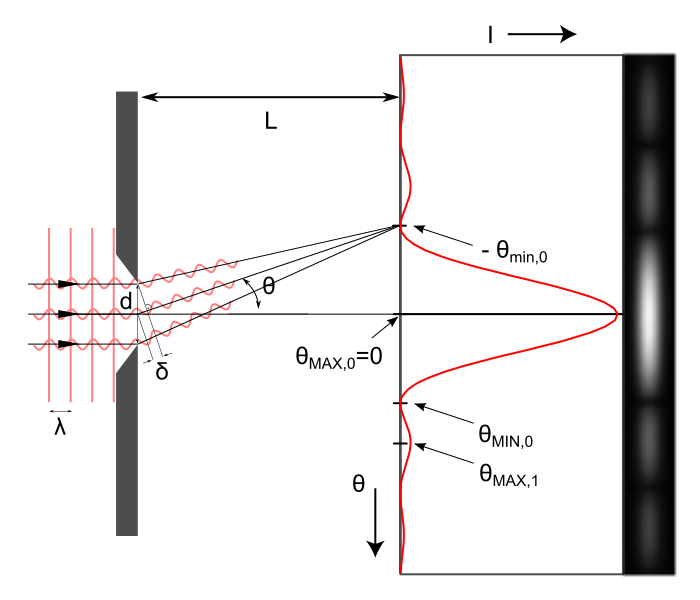
\includegraphics[]{Single.png}
% \caption{Single slit diffraction pattern and geometry. }
% \end{figure}

% The central peak has the greatest intensity, with decreasing intensity with each fringe either side. Each band/fringe has its greatest intensity in its centre. This is the point where light is most likely to fall in its range.
% The fringes are caused by the edges of the slit acting like two wave sources, the waves from the two wave "sources" interfere superimposing an interference pattern over the diffraction pattern.	 

% \section{Youngs experiment} 
% The modern double-slit experiment is a demonstration that light and matter can display characteristics of both classically defined waves and particles; moreover, it displays the fundamentally probabilistic nature of quantum mechanical phenomena. A simpler form of the double-slit experiment was performed originally by Thomas Young in 1801. He believed it demonstrated that the wave theory of light was correct and his experiment is sometimes referred to as Young's experiment or Young's slits. The experiment belongs to a general class of "double path" experiments, in which a wave is split into two separate waves that later combine into a single wave. Changes in the path lengths of both waves result in a phase shift, creating an interference pattern.
% \begin{figure*}
% \begin{tikzpicture}
% \tikzset{waveo/.style={decorate, draw=red,
%         decoration={complete sines,amplitude=20pt, segment length=10pt, start up, end up}}}
% \tikzset{wavet/.style={decorate, draw=blue,
%         decoration={complete sines,amplitude=20pt,start up, end up, segment length=10pt}}}
%         \tikzset{wavetr/.style={decorate, draw=blue,
%         decoration={complete sines,amplitude=20pt,start up, end down, segment length=10pt}}}
% \draw (0,0) -- (0,-.5);
% \draw (0,0) -- (0,.5);
% \draw (0,.8)-- (0,1.5);
% \draw (0,-.8)-- (0,-1.5);
% \draw[dashed] node [anchor=north east]{A} (0,.65)-- (10,0)node[anchor=west,text width=4cm]{Constructive interference. Path lengths $=n\lambda$};
% \draw[waveo] (0,.65)-- (10,0);
% \draw[waveo] (0,-.65)-- (10,0);
% \draw[thick] (10,2)--(10,-3);
% \draw[dashed] (0,.65)-- (10,-2);
% \draw[dashed] node [anchor=south east]{B}(0,-.65)-- (10,-2);
% \draw[wavetr] (0,.65)-- (10,-2) node[anchor=west, text width=4cm]{Destructive interference. Path lengths differ by $\frac{n}{2}\lambda$};
% \draw[wavet] (0,-.65)-- (10,-2);
% \draw[dashed] (0,-.65)-- (10,0) node[midway, fill=white]{Path};

% \end{tikzpicture}
% \caption{Constructive and destructive interference as a result of path differences.}
% \end{figure*}

% The position of the bright and dark fringes is determined by the geometry of the experimental set-up.The distance from center to bright spot n is:
%  \[y = \frac{n \lambda D}{d}\]
% We know that the maxima will be at angles such that the path difference will be whole number of wavelengths. The geometric derivation is shown below.\syl{describe an experimental demonstration of two-source interference for light, appreciating the historical importance of Young's experiment, and be familiar with experiments which demonstrate two source interference for water waves, sound waves and microwaves;} 

% \begin{figure}[!ht]
% 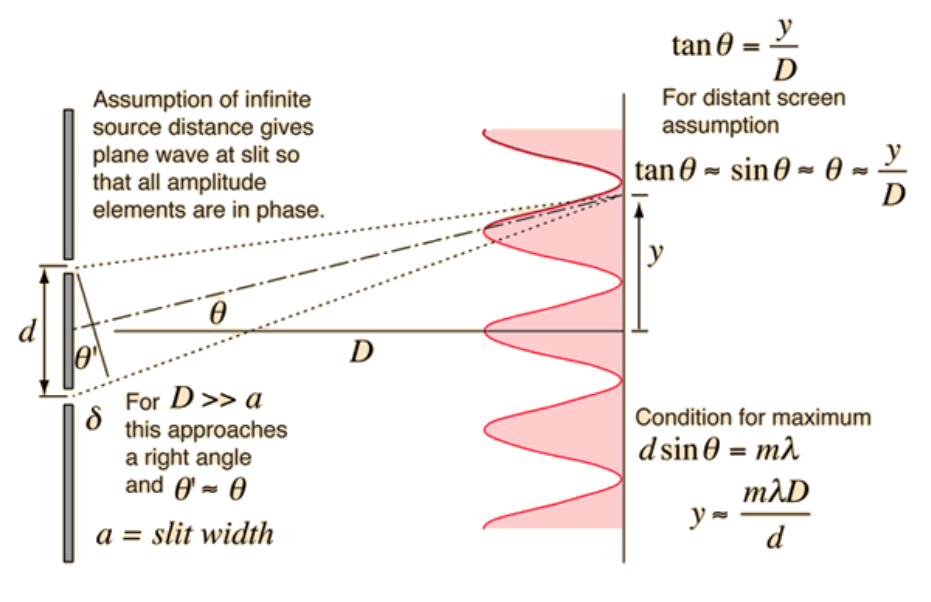
\includegraphics[]{twin.PNG}
% \caption{Beam pattern and geometric workings for Young's slits}
% \end{figure}

% Note that this makes use of the small angle approximation, a useful simplification of the basic trigonometric functions which is approximately true in the limit where the angle approaches zero.\begin{marginfigure}
% 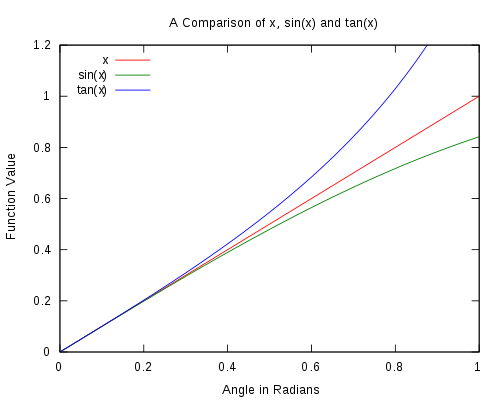
\includegraphics[]{small.png}
% \caption{Illustrating the small angle approximation}
% \end{marginfigure} They are truncations of the Taylor series for the basic trigonometric functions to a second-order approximation.

% \section{Diffraction grating}

% A diffraction grating is usually a piece of glass or plastic with closely-spaced lines on it. A transmission grating has thin clear spaces/slits where light can pass through, while a reflection gratings have shiny surfaces between the lines that reflect light.
% The tracks on a compact disc are very close together - the shiny gaps between the lines act as a reflection grating, leading to a colourful light spectrum being formed when light reflects off the surface.
% Transmission gratings are used to measure wavelengths of light to a very high degree of accuracy (spectrometer) - all substances have characteristic absorption/emission spectra.

% \subsection{Explaining diffraction gratings:}

% The individual lines act like wave sources or thin slits - they produce diffracting waves which will then interfere. Destructive interference leads to cancellation in nearly all directions - there are a few very clearly defined directions where constructive interference occurs, leading to bright fringes. The direction of these fringes depends on the wavelength of light - the wavelength can thus be determined!

% \paragraph{Diffraction grating formula} 

% Parallel rays of monochromatic light of wavelength ``$\lambda$'' fall on a diffraction grating with slit separation/grating spacing ``d''.

% \begin{marginfigure}
% 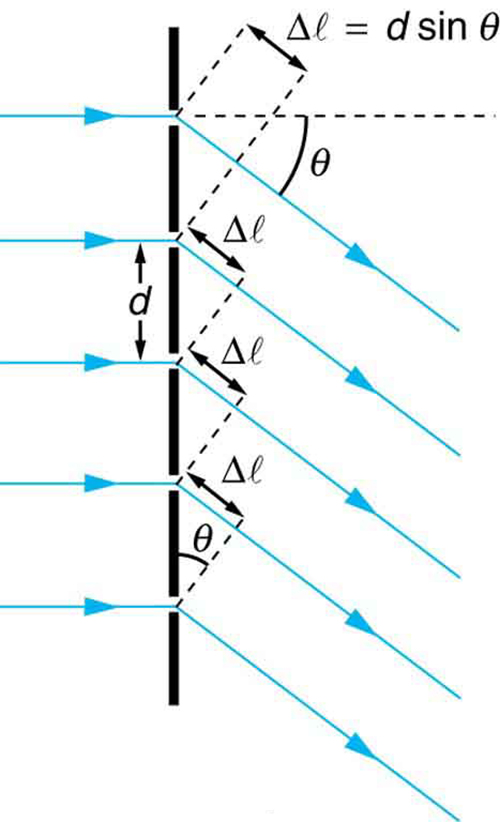
\includegraphics[scale=.5]{grating.jpg}
% \end{marginfigure}

% If the grating has $N$ lines per metre, the grating spacing is given by; $$d=\frac{1}{N}$$\syl{use the equation $d sin\theta = n\lambda$ for a diffraction grating}

% For constructive interference light from adjacent slits must be in phase (with light from all slits/lines).

% $\Delta l= d sin \theta$, where $\theta$ is the angle of diffraction

% Hence $$d sin\theta = n\lambda$$

% \section{Standing Waves}
% Standing or stationary waves\syl{understand that a stationary wave can be regarded as a superposition of two progressive waves of equal amplitude and frequency,travelling in opposite directions and that the internodal distance is $\frac{\lambda}{2}$}
%  are a superposition effect, which occurs when two identical waves (implying waves with a similar amplitude and frequency) travelling in opposite directions interfere.  The most common example of this is where incident and reflected waves interfere, for example on a spring or in a pipe in a musical instrument.

% With a string, spring or pipe of fixed length there will be certain frequencies where a standing wave pattern is produced as shown below.  These frequencies will be those which give an integral number of half wavelengths within the fixed length.  The standing wave is produced by interference of the waves travelling in both directions caused by reflection at the ends. See the diagram on the right.  

% It is characterised by nodes, which are points of zero displacement, and antinodes, which are points of maximum displacement.  The first few possible patterns for transverse waves on a string or spring are shown below.
% \begin{figure*}
% \begin{tikzpicture}[x={(1cm,0.5cm)},z={(0cm,1cm)},y={(1cm,-0.2cm)}]

%         %repere
%         \draw[->] (0,-pi,0) --++ (6,0,0) node[above right] {Frequency};
%         \draw[->] (0,-pi,0) --++ (0,6.5,0) node[right] {Time};
%         \draw[->] (0,-pi,0) --++ (0,0,1.5);        
%             %sinusoides
%             \draw[blue] plot[domain = -pi:+pi, samples = 300] 
%             (1,\x,{0.3*cos(10*.5/10*(\x) r)});
%             \draw[blue] (1,-pi-0.15,0) node [left]{$f_{0}$};
           
%             \draw[blue,dashed] plot[domain = -pi:+pi, samples = 300] 
%             (1,\x,{-0.3*cos(10*.5/10*(\x) r)});
%             \draw[blue] (0,-pi-0.15,0);
            
%             \draw[blue] plot[domain = -pi:+pi, samples = 300] 
%             (3,\x,{0.3*sin(10*1/10*(\x) r)});
%             \draw[blue] (3,-pi-0.15,0) node [left]{$f_{1}$};
%              \draw[blue,dashed] plot[domain = -pi:+pi, samples = 300] 
%             (3,\x,{-0.3*sin(10*1/10*(\x) r)});
%             \draw[blue] (3,-pi-0.15,0);
            
%             \draw[blue] plot[domain = -pi:+pi, samples = 300] 
%             (5,\x,{0.3*cos(10*1.5/10*(\x) r)});
%             \draw[blue] (5,-pi-0.15,0) node [left]{$f_{2}$};
%             \draw[blue,dashed] plot[domain = -pi:+pi, samples = 300] 
%             (5,\x,{-0.3*cos(10*1.5/10*(\x) r)});
%             \draw[blue] (5,-pi-0.15,0);
             
       
%     \end{tikzpicture}
% \end{figure*}  
% The separation of adjacent nodes or antinodes is half a wavelength.  The different numbers of half wavelengths on the spring or string correspond to different allowed frequencies.  The lowest of these (on the left) is called the fundamental.  The others are whole number multiples of the fundamental frequency and are called harmonics.  Each subsequent frequency is known as an overtone. Because of the phase change on reflection at the fixed ends the ends are both nodes.

% The wavelength can be found by measuring the node separation and doubling it.  This gives a method for finding the speed of sound or electromagnetic waves if the frequency is known, using v = f.  For example, if a standing wave is set up using 1 GHz radio waves and the node separation is found to be 0.15 m the wavelength will be 0.30 m and the wave speed is given by:

% $$c = f \times \lambda= (1 \times 10^{9} Hz) \times  0.30 m = 3 \times 10^{8} ms^{-1}$$

% \section{Standing Waves in Musical Instruments}

% Stringed instruments such as violins and pianos produce standing waves as described above.  Hitting, plucking or bowing the string produces waves, which travel off in both directions.  The pitch of the fundamental and therefore of the harmonics may be increased by reducing the length of the string, by increasing the tension in it or by using a lighter string.

% Wind instruments work by setting up longitudinal standing waves in tubes.  Examples are organ pipes, trumpets and clarinets.

 
% If the tube is open at one end and closed at the other there will be a node at the closed end and an antinode at the open end.  At the fundamental frequency the length of the tube is therefore 1/4 of a wavelength.  Harmonics occur at frequencies where the length of the tube is 3/4, 5/4, 7/4 etc wavelengths.closed
% \begin{marginfigure}
% 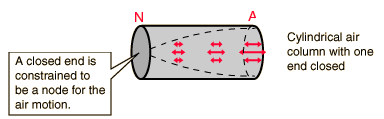
\includegraphics[]{closedpipe.png}
% \end{marginfigure}
% When any musical instrument is played the note you hear is at the fundamental frequency but a number of harmonics are also present.  The relative intensity of the different harmonics determines the quality of the note you hear.  It is this, which enables us to distinguish the same note played on different instruments.

% If the tube is open at both ends both ends have an antinode and the fundamental occurs when the tube length is half a wavelength.  Harmonics are at whole number multiples of the fundamental frequency. \begin{marginfigure}
% 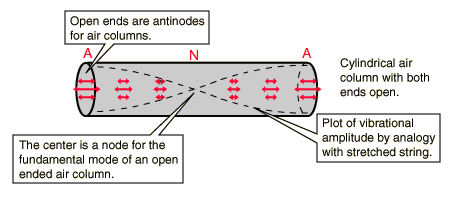
\includegraphics[]{openpipe.png}
% \end{marginfigure}

% \begin{figure}
% 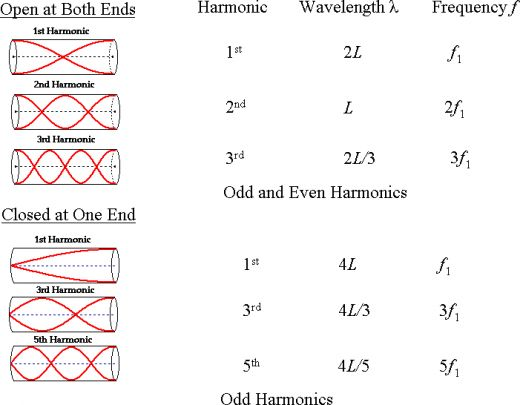
\includegraphics[]{pipes.jpg}
% \end{figure}
 
% \section{Refraction of Light}

% The Snell's Law equation is written in such a way as to emphasise symmetry. It is used to predict the change in direction that results from a change in velocity.\\
% \begin{figure*}
% \centering
% \begin{tikzpicture}[
%     media/.style={font={\footnotesize\sffamily}},
%     wave/.style={
%         decorate,decoration={snake,post length=1.4mm,amplitude=2mm,
%         segment length=2mm},thick},
%     interface/.style={
%         % The border decoration is a path replacing decorator. 
%         % For the interface style we want to draw the original path.
%         % The postaction option is therefore used to ensure that the
%         % border decoration is drawn *after* the original path.
%         postaction={draw,decorate,decoration={border,angle=-45,
%                     amplitude=0.3cm,segment length=2mm}}},
%    scale=1.2]
%     % Round rectangle
%     \fill[gray!10,rounded corners] (-4,-3) rectangle (4,0);
%     % Interface
%     \draw[blue,line width=.5pt,interface](-4,0)--(4,0);
%     % Vertical dashed line
%     \draw[dashed,gray](0,-3)--(0,3);
%     % Coordinates system
%     \draw(0,0.15)node[above]{$x$};
%     \draw[<->,line width=1pt] (1,0) node[above]{$y$}-|(0,-1) node[left]{$z$};
%     % Incidence
%     \draw[->,wave]
%          (150:4.5cm)--(150:3.5cm)node[right]{Incident ray};
%     \draw[gray](0:0cm)--(155:2cm);
%     \path (0,0)++(113:1cm)node{$\phi$};
%     \draw[->](0,0.75)arc(90:155:.75cm);
%     % Transmission
%     \draw[->,wave]
%          (-60:2.5cm)--(-60:3.5cm)node[right]{Refracted ray};
%     \draw[gray](0:0cm)--(-60:2cm);
%     \path (0,0)++(-70:1cm)node{$\theta$};
%     \draw[->] (0,-0.75) arc (-90:-60:.75cm);
  
%     % Media names
%     \path[media] (-3,.6)  node {media 1}
%                  (-3,-.6) node {media 2};

%     % $x$ axis
%     \filldraw[fill=white,line width=1pt](0,0)circle(.12cm);
%     \draw[line width=.6pt] (0,0)
%                           +(-135:.12cm) -- +(45:.12cm)
%                           +(-45:.12cm) -- +(135:.12cm);
%     % Interface pointer
%     \draw[-latex,thick](3.2,0.5)node[right]{$\mathsf{S_{1,2}}$}
%          to[out=180,in=90] (3,0);
         
%        \node at (0,-4){\begin{large}$\text{Snell's Law}=\frac{\sin\phi}{\sin\theta} = \frac{v_1}{v_2} = \frac{n_2}{n_1}$\end{large}};
%     % To-paths are really useful for drawing curved lines. The above
%     % to path is equal to:
%     %
%     % \draw[-latex,thick](3.2,0.5)node[right]{$\mathsf{S_{1,2}}$}
%     %      ..controls +(180:.2cm) and +(up:0.25cm) .. (3,0);
%     % Internally the to path is translated to a similar bezier curve,
%     % but the to path syntax hides the complexity from the user. 
% \end{tikzpicture}
% \caption{Refraction from low refractive index to higher refractive index (eg. Air to glass)}
% \end{figure*}
% Looking at the equation for snell's law we see that there must be a point at which the incident ray causes a refraction at, or above 90 degrees. This is called the \textbf{\textit{critical angle}}. At shallower angles of incidence, total internal reflection occurs.
% The only application of total internal reflection required to be learnt is the step-index multimode (`thick core') optical fibre. Step-index means simply that the core is glass of one refractive index and the cladding is glass of a lower index (students need to know why it has to be lower), with an abrupt change in index at the interface.
% \begin{figure*}
% \centering
% \begin{tikzpicture}[scale=1]
% \shade[left color=black!40!white,right color=black!10!white](0,-2.5)--(10,-2.5)--(10,2.5)--(0,2.5)--cycle;
% \draw[dashed, thin, red](-1,0)--(11,0);
% \draw[thin](0,-2.50)--(0,2.5);
% \draw(0,2)--(10,2);
% \draw(0,2.5)--(10,2.5);
% \draw(0,-2)--(10,-2);
% \draw(0,-2.5)--(10,-2.5);
% \draw[thick, blue,->](-1.8,-1)--(0,0)--(2,2)node(A){}--(6,-2)--(9.5,2);
% \draw[dashed, thin](2,1)--(2,3)node[]{};
% \node at (1,2.25){$n_2$};
% \node at (1,-1.75){$n_1$};
% \draw[->](2,1.4)arc(-90:-125:.75cm)node[anchor=north,midway]{$\theta_i$};
% \draw[->](2,2.75)arc(90:-40:.75cm)node[anchor=south,midway]{$\theta_r$};
% \node at (7,3.25){$n_1 \sin{\theta_i}=n_2 \sin{\theta_r}$};
% \node at (9,-1.75){\tiny Core};
% \node at (9,-2.35){\tiny Cladding};
% \begin{scope}
% \path[clip,decoration={random steps, segment length=6pt, amplitude=3pt},decorate] (9.9,-2.6)--(9.9,2.6)--(11,2.6)--(11,-2.6)-- cycle; 
% \shade[left color=white,right color=white](9.9,-3)--(9.9,3)--(11,3)--(11,-3)-- cycle;
% \end{scope}
% \end{tikzpicture}
% \caption{Total internal reflection in a single fibre}

% \end{figure*}
% While such fibres are fine for conveying light for illumination, students need to know that they can't be used for transmitting a rapid sequence of data over a long distance. Multimode dispersion is the problem.
% \begin{figure*}
% \centering
% \pgfmathdeclarefunction{gauss}{2}{%
%   \pgfmathparse{1/(#2*sqrt(2*pi))*exp(-((x-#1)^2)/(2*#2^2))}%
% }
% \begin{tikzpicture}[scale=1]

% \shade[left color=black!40!white,right color=black!10!white](0,-2.5)--(10,-2.5)--(10,2.5)--(0,2.5)--cycle;
% \draw[dashed, thin, red](-1,0)--(10,0);
% \draw[thin](0,-2.50)--(0,2.5);
% \draw(0,2)--(10,2);
% \draw(0,2.5)--(10,2.5);
% \draw(0,-2)--(10,-2);
% \draw(0,-2.5)--(10,-2.5);
% \draw[thick, blue,->](-1.8,-1)--(0,0)--(2,2)--(6,-2)--(9.5,2);
% \draw[thick, cyan,->](-2.2,-1)--(0,0)--(2.3,2)--(6.6,-2)--(10.9,2);
% \draw[dashed, thin](2,1)--(2,3)node[]{};
% \draw[dashed, thin](2.3,1)--(2.3,3)node[]{};
% \node at (1,2.25){$n_2$};
% \node at (1,-1.75){$n_1$};
% \node at (9,-1.75){\tiny Core};
% \node at (9,-2.35){\tiny Cladding};
% \node at (12,-3.25){\tiny{Broad pulse}};
% \node at (-3,-3.25){\tiny{Defined pulse}};
% \begin{scope}
% \path[clip,decoration={random steps, segment length=6pt, amplitude=3pt},decorate] (9.9,-2.6)--(9.9,2.6)--(11,2.6)--(11,-2.6)-- cycle; 
% \shade[left color=white,right color=white](9.9,-3)--(9.9,3)--(11,3)--(11,-3)-- cycle;
% \end{scope}

% \begin{axis}[scale=.5,
%     anchor=origin,
%     at={(-3cm,-3cm)},
%     style={samples=51,smooth},
%     hide axis
% ]
% \addplot[mark=none,thick] {gauss(0,.4)};
% \end{axis}
% \begin{axis}[scale=.5,
%     anchor=origin,
%     at={(12cm,-3cm)},
%     style={samples=51,smooth},
%     hide axis
% ]
% \addplot[mark=none,thick] {gauss(0,2)};
% \end{axis}

% \draw[thick, blue,->](-1.8,-1)--(0,0)--(2,2)--(6,-2)--(9.5,2);
% \draw[thick, cyan,->](-2.2,-1)--(0,0)--(2.3,2)--(6.6,-2)--(10.9,2);
% \end{tikzpicture}
% \caption{Multi-mode dispersion in a fibre resulting from the two different length paths}
% \end{figure*}

% Light travelling at an angle to the axis of the fibre will travel further for a given axial length of fibre, than light travelling parallel to, or at a smaller angle to, the axis, and so will arrive later. Thus the arrival time of an element of data encoded in the light is smeared out. The element could start to arrive (by the shortest route) earlier than the previous element has finsished arriving by its longest route. Even worse confusion can occur. 
% There are two ways round the problem of multimode dispersion\ldots
% \begin{itemize}
% \item Make fibres with graded index cores. This means cores which have a progressively lower index as we go out from the axis towards the interface with the cladding. The lower the index the faster the light travels so, if the grading is correctly calculated, the longer, more zigzaggy, paths cash in on the `faster medium' and take no longer than the short, axial, route. Clever stuff, but note that graded index fibres are not in the WJEC specification. 
% \item Make the core very thin. Its diameter must  be no more than a few wavelengths of the light (or infrared) being carried. Such fibres are monomode. Light travels parallel to the axis. There are no zigzag modes. Students are required to know this. You are not required to know why very thin fibres are monomode. This is just as well, because it cannot be shown by ray optics, nor even by simple application of Huygens Principle. Electromagnetic wave theory is needed.
% \end{itemize}
% The website\\ \url{http://www.techoptics.com/pages/Fiber\%20Optics\%20-\%20Optical\%20Fiber.html}   \\ 
% gives an excellent summary of fibres for data transmission, with some facts and figures.

% \section{Photons}

% Everything in nature seems to come in lumps or quanta (singular: quantum). For example, ordinary matter is made of atoms, and electric charge comes in units of e. This lumpiness was only becoming fully accepted a hundred years ago. But in 1905 Einstein made the bold suggestion that light, too, was `lumpy'. Light quanta are now called photons.
% A photon is a discrete packet of electromagnetic radiation energy. The energy of a photon is given by
% $$ E=hf $$
% In which $f$ is the frequency of the light and $h$ is a constant called Planck's constant. $h = 6.6 \times 10^{-34} \text{Js}$ \sidenote{For interest only \ldots The constant h had first arisen in the earlier (1900) work of Max Planck on the radiation inside a cavity with hot walls. Planck had shown that the energies of oscillating particles in the wall seemed to be quantised.}

% Einstein suggested some experiments in which the quantisation of light should reveal itself. The simplest to understand involved the photoelectric effect, a phenomenon known about since the late 1880s.

% \section{Laser Physics}
% Lasers, by now, are in nearly every household as they were once in every self-respecting science fiction film. Although, the death ray mystique will appeal to most A-level students there is real value in studying the physics which forms the foundation of laser construction. Unlike other subjects such as relativity or nuclear physics which can only be touched upon within an A-level course, the essential physics underpinning lasers can be taught reasonably well in a few lessons. Also, these fundamentals of lasers can be taught at the right level while not oversimplifying the subject.

% LASER is an acronym and stands for Light Amplification by Stimulated Emission of Radiation. Which leads us nicely onto what is stimulated emission?

% \subsection{The Three Important Atomic Processes}
% These three processes are:
% \begin{enumerate}
% \item Absorption of light
% \item Spontaneous emission of light
% \item Stimulated emission of light
% \end{enumerate}
% Absorption of light by an atom is shown in the diagram below - a photon of the correct energy is absorbed by the atom and an electron gains enough energy to move from the ground state to the excited state (Note: for the moment we are only considering the ground state and the first excited state only).

% \begin{figure*}
% \usetikzlibrary{shadings}
% \centering
% \begin{tikzpicture} [scale=.7, wave/.style={
%         decorate,decoration={snake,post length=1.4mm,amplitude=2mm,
%         segment length=2mm},thick},
%     interface/.style={
%         % The border decoration is a path replacing decorator. 
%         % For the interface style we want to draw the original path.
%         % The postaction option is therefore used to ensure that the
%         % border decoration is drawn *after* the original path.
%         postaction={draw,decorate,decoration={border,angle=-45,
%                     amplitude=0.3cm,segment length=5mm}}} ]
   
% \pgfdeclareverticalshading{rainbow}{100bp} 
%  {color(0bp)=(red); color(25bp)=(red); color(35bp)=(yellow); 
%   color(45bp)=(green); color(55bp)=(cyan); color(65bp)=(blue); 
%   color(75bp)=(violet); color(100bp)=(violet)}
%     \begin{scope}[]
%         \shade[shading=rainbow]
%             (0,0) rectangle (3,8); 
%     \draw[very thick,black] (0,3) -- (3,3);
%     \draw[very thick,black] (0,6.3) -- (3,6.3);
%      \end{scope}
% \draw[thick, black] (3.5,-1)--(10,-1);
% \draw[thick, black] (3.5,3)--(10,3);
% \draw[thick, black] (3.5,6.3)--(10,6.3);
% \draw[dashed,<-]  (5,6.3)--(5,-1);
% \draw[dashed,<-]  (7,3)--(7,-1);
% \draw[wave,blue,->](-2,8.5)--(5,3.5);
% \draw[wave,green,->](-1,6)--(7,1);
% \draw [fill=black] (5,-1) circle (2mm);
% \draw [fill=black] (7,-1) circle (2mm);
%     \end{tikzpicture}
%     \caption{Absorption of light. The photon energy has to correspond to a possible energy level transition for the energy to be absorbed by an electron.}
% \end{figure*}
 
% Spontaneous emission is the reverse process - an electron drops spontaneously (and randomly) from the excited state to the ground state and emits a photon of the same energy. These photons have random phase and random direction.

% \begin{figure*}
% \usetikzlibrary{shadings}
% \centering
% \begin{tikzpicture} [scale=.7, wave/.style={
%         decorate,decoration={snake,post length=1.4mm,amplitude=2mm,
%         segment length=2mm},thick},
%     interface/.style={
%         % The border decoration is a path replacing decorator. 
%         % For the interface style we want to draw the original path.
%         % The postaction option is therefore used to ensure that the
%         % border decoration is drawn *after* the original path.
%         postaction={draw,decorate,decoration={border,angle=-45,
%                     amplitude=0.3cm,segment length=5mm}}} ]
   
% \pgfdeclareverticalshading{rainbow}{100bp} 
%  {color(0bp)=(red); color(25bp)=(red); color(35bp)=(yellow); 
%   color(45bp)=(green); color(55bp)=(cyan); color(65bp)=(blue); 
%   color(75bp)=(violet); color(100bp)=(violet)}
%     \begin{scope}[]
%         \shade[shading=rainbow]
%             (0,0) rectangle (3,8); 
%     \draw[fill=black] (0,0) rectangle (3,3);
%     \draw[fill=black] (0,3.1)rectangle (3,5); 
% \draw[fill=black] (0,5.1)rectangle (3,8); \end{scope}
% \draw[thick, black] (3.5,0)--(10,0)node[anchor=west]{Ground State};
% \draw[thick, black] (3.5,3)--(10,3)node [anchor=west]{$2.32eV$};
% \draw[thick, black] (3.5,5)--(10,5) node [anchor=west] {$2.75eV$};
% \draw [fill=black] (5,5) circle (2mm);
% \draw [fill=black] (7,3) circle (2mm);
% \draw[dashed,->]  (5,5)--(5,0);
% \draw[dashed,->]  (7,3)--(7,0);
% \draw[wave,blue,->](5,2)--(8,2)node[anchor=west]{$\lambda=?$};
% \draw[wave,green,->](7,1)--(10,1)node[anchor=west]{$\lambda=?$};
 
%     \end{tikzpicture}
%     \caption{Emission spectra and corresponding energy levels. Note: the frequency and wavelength can be calculated from the change in energy of the electron using $E=hf$}
% \end{figure*}
% However, there is also a third process [which was originally proposed by Einstein in 1917]. This process is known as stimulated emission - an electron is `stimulated' to drop from its excited state by an incoming photon. 

% \begin{figure}
% 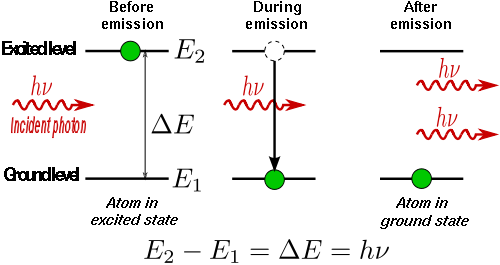
\includegraphics[scale=.5]{stimem.png}
% \caption{Stimulated emission - an incoming photon of an energy matching the transition can cause an electron to drop to a lower energy level. In order to do this it must release a photon identical to the first.}
% \end{figure}

% The reason that the electron is stimulated to drop is that the incoming photon is an electromagnetic wave and its e-m field will exert an oscillating force on the excited electron. If the incoming photon is of the correct frequency, this oscillating force will cause the excited electron to drop and both photons will exit with the same frequency, phase and direction. Note: again, the incoming photon needs to be of the correct energy.

% \subsection{Inverting The Population}
% In order to get as much light out of a system as is possible we need to get as many atoms excited as is possible.\begin{marginfigure}
% 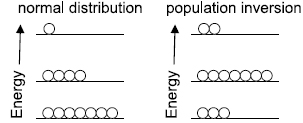
\includegraphics[]{popin.jpg}
% \caption{Population inversion - when more electrons are in an excited state than in the ground state. This is the opposite of a `normal' situation}
% \end{marginfigure} Obviously, the more electrons we have in an excited state the more will drop and emit photons (either spontaneously or through stimulation). However, there is one serious problem that arises when we produce a lot of light - the very photons that we produce are the actual photons that can be absorbed (they have the correct energy to produce both effects). If we have photons being absorbed all the time then our laser beam isn't getting any stronger.

% Forget, for the moment about spontaneous emission (we are allowed to but we'll explain why later). When a photon arrives at an atom one of three things can happen:
% \begin{enumerate}
% \item It can pass by and do nothing.
% \item It can be absorbed (if the atom is in the ground state).
% \item It can cause stimulated emission (if the atom is in the excited state).
%  \end{enumerate}
% When it comes to producing a laser beam with a high intensity the three options above will have the following effect on the beam.
% \begin{enumerate}
% \item No change in the beam.
% \item Net loss of one photon from the beam.
% \item Net gain of one photon in the beam.
% \end{enumerate}
% We need to arrive at a situation where stimulated emission is more likely than absorption so that the laser beam increases in intensity. Since stimulated emission occurs if the electrons are in the upper level and absorption when electrons are in the lower level we need to get more electrons into the upper, excited level. This is called population inversion (or $N_{2} > N_{1}$ as stated in the syllabus, where $N_2$ and $N_1$ are the number of electrons in the excited state and the ground state respectively).

% Unfortunately, this goes against what happens in nature - lower energy levels are always more heavily populated than higher energy levels when we have thermal equilibrium. There's only one thing for it - get rid of this thermal equilibrium. How do we do this? We continue to pump energy into exciting electrons to higher energy levels to maintain a population inversion and to break the conditions of thermal equilibrium.

% Population inversion is not usually possible if we only have two energy levels (if pumping is carried out by light).
%  \newpage
% \subsection{The 3 Energy Level Laser System}

% \begin{figure}
% 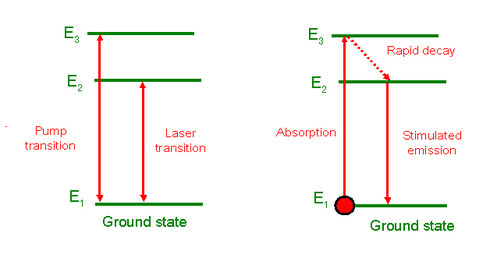
\includegraphics[]{lasers.jpg}
% \end{figure}
% \sidenote{Note:\begin{itemize} \item E3 (to E2) has to have a short lifetime because E3 cannot start to fill up - pumping won't then be possible. Also, we don't want the electrons to stay in E3 and have them stimulated to drop back to E1 by the pumping light - that's back to the 2-level system again which wasn't quite good enough.

% \item More than half the electrons from E1 must be pumped to E2 (via E3) in order to obtain a population inversion - that's a lot of electrons!\end{itemize}}
% \begin{enumerate}
% \item Pumping. Electrons are promoted from the ground state (E1) to E3 usually by using an external light source or by electron collisions.
% \item Electrons drop quickly (because E3 is chosen to have a short lifetime of the order of nanoseconds) to the metastable (E2). Calling E2 metastable means that it has a long lifetime and electrons stay there for a long time (not that long really around a millisecond but that's a very long time for an electron).
% \item This is the transition that produces the laser photons so we must have N2 > N1. Note that, although stimulated emission still reduces our population inversion, the pumping is at a different wavelength. We have to make sure that the pumping [1] exceeds the stimulated emission [3] to maintain a population inversion.
% \end{enumerate}

% \subsection{The 4 Energy Level Laser System}

% \begin{figure*}
% 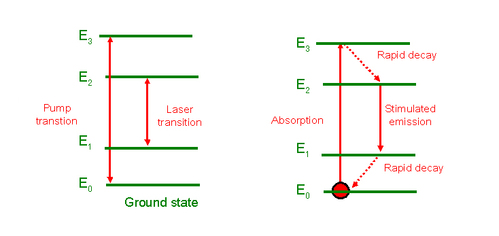
\includegraphics[]{fourlevel.jpg}
% \end{figure*}
% \begin{enumerate}
% \item Pumping again.
% \item Quick drop to the metastable state E2.
% \item This is the laser light producing transition so this time N2 > N1. However, because E0 is the ground state, E1 is practically empty initially so obtaining population inversion is far, far easier (definitely no need to pump half the electrons!).
% \item Another quick transition so E1 has a short lifetime. This is because we want E1 to be empty so that we have a population inversion (if N1 is small it's easier for N2 to be larger than N1).							
%  \end{enumerate}
% \subsection{Laser Construction}

% \begin{figure*}
% 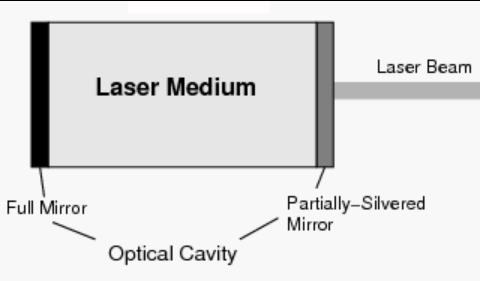
\includegraphics[scale=.5]{lasercav.PNG}
% \end{figure*}

% In order to ensure that the laser produces light of a high enough intensity, the above set up is used. The amplifying medium is the region where the population inversion exists. This means that the conditions are right in the amplifying medium for stimulated emission. Under these conditions one photon has the potential to produce two photons and these can produce 4 photons, then 8 photons etc. Like a chain reaction, this process will lead to an exponential increase in output energy. Laser physicists aren't happy with this, they go even further - they use mirrors to ensure that this exponential increase happens many times. Because only 1\% of the light exits each time it reflects back and forth between the mirrors, on average, the beam will pass through the amplifying medium a hundred times before it exits. Now, considering that each time the beam passes through the amplifying medium it is increasing exponentially, this factor of 100 makes an enormous difference. 

% This all leads to very high light intensities inside the amplifying medium and this is why (as was said earlier) we can forget about spontaneous emission. Imagine that you're an excited electron sitting happily in your higher energy level. Normally, you'll just drop down spontaneously when your time is up. But, inside a laser, there's so much light that you never drop spontaneously because before your time's up you've been disturbed by another photon, stimulated to join in with all the other light and join in coherently as well!

% \subsection{Efficiency}
% Usually, lasers are very inefficient beasts. Because of the large energies required to maintain a population inversion, their efficiencies are generally far below 1\%. Some reasons for this:
% \begin{itemize}
% \item The pumping energy is considerably larger than the output photon energy.
% \item High intensity pumping combined with the high intensity of the laser beam means that the amplifying medium will get very hot. So, there will be large heat losses. To make this matter worse, we need to cool the amplifying medium usually so that it, or its container, doesn't melt. By cooling the system we just transfer more heat and increase our losses but better this than destroy a \textsterling 50 000 laser!
% \end{itemize}
 
% \subsection{Semiconductor Lasers}
% The basic structure of a standard `edge emitting' semiconductor laser is shown below. The whole block shown below is a semiconductor chip with dimensions approximately 0.5mm $\times$ 0.5 mm $\times$ 1 mm.
% \begin{figure*}
% 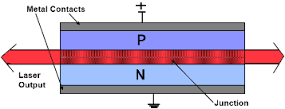
\includegraphics[]{diode.png}
% \end{figure*}

 
% The above laser fits the basic shape of a normal laser, the mirrors, however, are far from the 100\% and 99\% reflecting ideals discussed earlier. The mirrors are simply due to the semiconductor-air boundary at the edges of the chip. [This in fact gives 40\% reflection only (at both sides).] This would be disastrous for highly inefficient gas lasers but not for our semiconductor laser. The reason why:
% \begin{itemize}
% \item The population inversion inside the semiconductor sandwich area is millions of times higher than in gas lasers [$10^{25}$ electrons/$m^{3}$].
% \item The exponential increase in light intensity (i.e. 1 photon becoming two, becoming four etc.) occurs far more quickly because of the higher population inversion.
% \item So the fact that we lose 60\% of the light at each reflection is compensated for by having huge gains between the mirrors.
%  \end{itemize}

% \subsection{Advantages and Uses of Laser Diodes}
% These are straightforward and can be summarised as follows:

% Advantages:
% \begin{itemize}
% \item Cheaper
% \item Smaller
% \item More efficient
% \item Easy to mass produce	
% \end{itemize}
% Some uses:
% \begin{itemize}
% \item Inside DVD and CD players
% \item Bar-code readers
% \item Telecommunications (via optical fibres)
% \item Image scanning
% \item Laser surgery
% \end{itemize}
% The usefulness of laser diodes is `reflected' in the number of them produced annually - around 1 billion (109) laser diodes are produced worldwide per year!
 
% For more than enough further reading see:
% \begin{itemize}
% \item \url{http://members.aol.com/WSRNet/tut/ut1.htm}
% \item Wikipedia \url{http://en.wikipedia.org}  then type `laser' or `semiconductor laser'
% \item Google search `laser theory'
% \end{itemize}

	
\subsection*{Wave terminologies}

\begin{marginfigure}
	\vspace*{-12pt}
	\centering
	\begin{tikzpicture}[scale=0.78]
	\draw[help lines, gray!50, very thin, step=0.2] (0,-2) grid (6,2);
	\draw[help lines, step=1] (0,-2) grid (6,2);
	\foreach \y in {-2,-1,0,1,2} \node[left] at (0,\y) {$\y$};
	\foreach \x in {0,0.1,0.2,0.3,0.4,0.5,0.6} \node[below] at (10*\x,-2) {$\x$};
	\node at (-1.2,1.5) {$y$/cm};
	\node at (5,-2.8) {$x$/m};
	\draw [thick, blue, domain=0:6, samples=30, smooth] plot (\x,{1.6*sin(75*\x)});
	\draw [thick, Green, domain=0:6, samples=30, smooth] plot (\x,{-0.8*cos(120*\x)});
	\node[blue] at (1.8, 1.6) {$P$};
	\node[Green] at (4.5, 1.1) {$Q$};
	\end{tikzpicture}
	\vspace*{-18pt}
\end{marginfigure}

\subsection*{transverse \& longitudinal waves}

\begin{marginfigure}
	\vspace*{-12pt}
	\centering
	\begin{tikzpicture}[xscale=0.6,yscale=0.75]
	\draw [->] (0,-2) -- (0,2.4) node[midway,left]{$O$} node[left]{$y$};
	\draw [->] (0,0) -- (2.5*pi,0) node[below]{$x$};
	\draw[very thick,->] (1.6*pi,2) -- (2.4*pi,2);
	\node[above,twoline] at (2*pi, 2.2) {direction of\\wave motion};
	\draw [thick, blue, domain=0:2.4*pi, samples=30, smooth] plot (\x,{1.6*sin(\x*1.2 r)});
	\draw[fill, red] (5*pi/12,1.6) circle (0.08) node[above, black]{$P$};
	\draw[fill, red] (10*pi/12,0) circle (0.08) node[above right, black]{$Q$};
	\draw[fill, red] (15*pi/12,-1.6) circle (0.08) node[below, black]{$R$};
	\draw[fill, red] (20*pi/12,0) circle (0.08) node[above left, black]{$S$};
	\end{tikzpicture}
	\vspace*{-16pt}
\end{marginfigure}

\subsection*{Sound waves}

\subsection*{Electromagnetic waves}

%\question{
%	Suppose a sound wave and an electromagnetic wave have the same wavelength, compare their frequencies.
%}

\subsection*{Intensity of waves}

\subsection*{Polarisation}

\subsection*{Diffraction}

\subsection*{Doppler effect}

For the questions below, take the speed of sound to be $340 \mps$.

\cleardoublepage

% ===== Chapter: superposition =====
\section{Superposition of Waves}

When two of more waves meet together, the resultant motion is a combination of the individuals. They can form a \emph{resultant wave} when they overlap, after which they cross one another and neither is affected. In this chapter, we will study the principle of superposition, and look at two important consequences: the phenomenon of \emph{interference} and \emph{stationary waves}.

\subsection{Superposition of waves}

\subsection{Principle of superposition}

\begin{ilight}
	 When two (or more) waves meet to form a resultant wave, the \keypoint{principle of superposition} states that the resultant displacement is the vector sum of each individual displacement\index{superposition of waves!principle of superposition}
\end{ilight}

\begin{figure*}[ht]
	\centering
	\begin{minipage}{0.45\textwidth}
		\centering
		\begin{tikzpicture}[scale=0.8]
		\draw [->] (0,-2) -- (0,2) node[above]{displacement};
		\draw [->] (0,0) -- (6.4,0) node[below]{$t$};
		\draw [Green, dashed] (0,0) --++ (0.8,1) --++ (1.6, -2) --++ (1.6,2) --++ (1.6, -2) --++ (0.4,0.5) node[below right]{$A$};
		\draw [purple, dashed] (0,-0.8) -- (1.6,-0.8) -- (2.4, 0.4) -- (4 ,0.4) -- (4.8, -0.5) -- (5.6, -0.5) -- (6, 0.4) node[right]{$B$}; 
		\draw [thick, blue] (0,-0.8) -- (0.8, 0.3) -- (1.6, -0.8) -- (2.4, -0.6) -- (4, 1.4) -- (4.8, -0.5) -- (5.6, -1.5) -- (6,0.1);
		\end{tikzpicture}
	\end{minipage}\hfil
	\begin{minipage}{0.45\textwidth}
		\centering
		\begin{tikzpicture}[scale=0.8]
		\draw [->] (0,-2) -- (0,2) node[above]{displacement};
		\draw [->] (0,0) -- (6.4,0) node[below]{$t$};
		\draw [Green,dashed,domain=0:6,samples=30,smooth] plot (\x,{0.6*sin(\x*3 r)}) node[below right]{$A$};
		\draw [purple,dashed,domain=0:6,samples=30,smooth] plot (\x,{1.2*sin(\x*1.5 r)}) node[above right]{$B$};
		\draw [thick,blue,domain=0:6,samples=30,smooth] plot (\x,{1.2*sin(\x*1.5 r) + 0.6*sin(\x*3 r)});
		\end{tikzpicture}
	\end{minipage}
\end{figure*}

Two important situations are constructive superposition and destructive superposition\index{superposition of waves!constructive superposition}\index{superposition of waves!destructive superposition}

\keypoint{Constructive superposition} occurs when resultant wave has greatest possible amplitude. This happens when peaks of the two waves meet together (also trough meets trough)\footnote{This statement is implicitly for transverse waves. For longitudinal waves to superpose constructively, the regions of compression (or rarefaction) must overlap.} 	peaks of both waves must arrive with a time difference $\Delta t = 0, \, T, \, 2T, \cdots$
	
\keypoint{Destructive superposition} occurs when amplitudes of each wave cancel out one another this happens when peak of one wave overlaps with trough of the other wave peaks of both waves must arrive with a time difference $\Delta t = \frac{1}{2}T, \, \frac{3}{2}T, \, \frac{5}{2}T, \cdots$

\begin{figure*}[ht]
	\centering
	\noindent\begin{minipage}{0.45\linewidth}
		\centering
		\begin{tikzpicture}[xscale=0.8, yscale=0.75]
		\draw [->] (0,-2) -- (0,2) node[above]{displacement};
		\draw [->] (0,0) -- (6.4,0) node[below]{$t$};
		\draw [Green, dashed,domain=0:6,samples=30,smooth] plot (\x,{0.6*sin(\x*1.2 r)});
		\draw [purple, dashed,domain=0:6,samples=30,smooth] plot (\x,{1.2*sin(\x*1.2 r)});
		\draw [thick,blue,domain=0:6,samples=30,smooth,variable=\x] plot (\x,{1.8*sin(\x*1.2 r)});
		\end{tikzpicture}
	\end{minipage}\hfil
	\begin{minipage}{0.45\linewidth}
		\centering
		\begin{tikzpicture}[xscale=0.8, yscale=0.75]
		\draw [->] (0,-2) -- (0,2) node[above]{displacement};
		\draw [->] (0,0) -- (6.4,0) node[below]{$t$};
		\draw [Green,dashed,domain=0:6,samples=30,smooth] plot (\x,{-1.2*sin(\x*1.2 r)});
		\draw [purple ,dashed,domain=0:6,samples=30,smooth] plot (\x,{1.6*sin(\x*1.2 r)});
		\draw [very thick,blue,domain=0:6,samples=30,smooth] plot (\x,{0.4*sin(\x*1.2 r)});
		\end{tikzpicture}
	\end{minipage}\hfil
	\caption{constructive and destructive superposition of two transvers waves}
\end{figure*}
\vspace{2cm}
Note: longitudinal waves are often represented by transverse diagrams. Transverse are much clearer and easier to read:
\vspace{1cm}
 

\begin{figure*}[htp]
	\centering
	\noindent\begin{minipage}{0.5\linewidth}
		\centering
		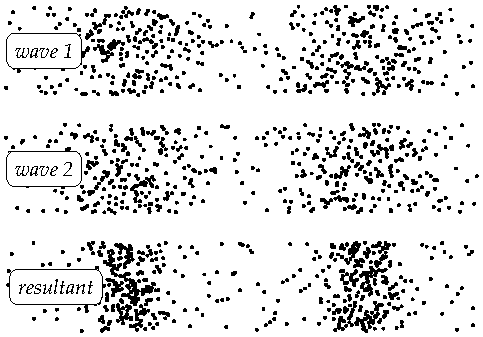
\includegraphics[width=.95\textwidth]{longitudinal+I.pdf}
	\end{minipage}\hfil
	\begin{minipage}{0.5\linewidth}
		\centering
		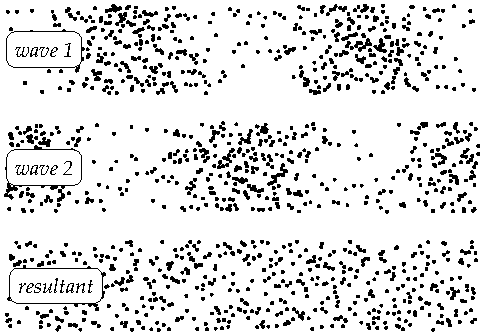
\includegraphics[width=.95\textwidth]{longitudinal-I.pdf}
	\end{minipage}
	\caption{constructive and destructive superposition of two sound waves} 
\end{figure*}

\subsection{Path difference}

The \keypoint{path difference}\index{path difference} is the difference in distance that two waves must travel from their sources to a given point. It plays a crucial role in wave interference, where waves can either constructively or destructively superpose depending on their path difference. Path difference is generally expressed in multiples of wavelength. To tell whether two waves superpose constructively or destructively:

{

\centering
\vspace*{6pt}
\begin{tcolorbox}[colframe=red, colback=yellow!30, width=0.65\textwidth]
	\setlength{\baselineskip}{\baselineskip}%
	
	\centering
	
	if ${\Delta L = 0, \, \lambda, \, 2\lambda, \cdots}$, then superposition is constructive
	
	if ${\Delta L = \frac{\lambda}{2}, \, \frac{3\lambda}{2}, \, \frac{5\lambda}{2}, \cdots}$, then superposition is destructive
	
\end{tcolorbox}\vspace*{-4pt}

}

\newpage

\subsection{Phase difference}

When two waves or two vibrating particles are compared, it is also useful to describe how much one is out of step with the other in terms of their \keypoint{phase difference}\index{phase difference} ($\Delta \phi$)
\footnote{More logically, we should first define the notion of \emph{phase angle} before talking about the \emph{phase difference}, which is simply the difference between the phase angles of two waves.
	
	Wave motion can generally be described by sine (or cosine) functions. Since the initial displacement of a wave is not necessarily zero, one can introduce a constant term that appears in the argument of the sine function. This term shifts the origin of the sine, and we call that the \emph{phase angle} $\phi$ of the wave, measured in radians (or degrees). One can think of $\phi$ as a number giving the fraction in a complete oscillation.
	
	In particular, the displacement $y$ of a transverse wave along the direction $x$ of energy transfer can be given by: $y = A \sin\left( \frac{2\pi x}{\lambda} - \frac{2\pi t}{T} + \phi \right)$. You can verify that this indeed describes a sinusoidal wave of wavelength $\lambda$ and period $T$ travelling at speed $v = \frac{\lambda}{T}$, while $\phi$ determines when and where the peaks show up.}

Phase difference is measured in radians (rad) or degrees ($^\circ$),  if two waves have a phase difference $\Delta \phi = 0,2\pi,4\pi,\cdots$, the two waves are said to be \keypoint{in phase}\footnote{If $\Delta \phi$ is given in degrees, then two waves are in phase if $\Delta \phi = 0, \, 360^\circ, \, 720^\circ, \cdots$}. In this case, peak of one wave overlaps with peak of the other. If two waves are not in phase, then they are said to be \keypoint{out of phase}
If $\Delta \phi = \pi, 3\pi, 5\pi, \cdots$, then two waves are completely out of phase, or \keypoint{anti-phase}\footnote{If $\Delta \phi$ is given in degrees, then two waves are anti-phase if $\Delta \phi = 180^\circ, \, 540^\circ, \, 900^\circ, \cdots$} in this case, peak of one wave meets the trough of the other. 

We can tell whether two waves superpose constructively or destructively from their phase difference as follows:

{
	
	\centering
	\vspace*{6pt}
	\begin{tcolorbox}[colframe=red, colback=yellow!30, width=0.65\textwidth]
		\setlength{\baselineskip}{\baselineskip}%
		
		\centering
		
		if ${\Delta \phi = 0, \, 2\pi, \,4\pi, \cdots}$, then superposition is constructive
		
		if ${\Delta \phi = \pi, \, 3\pi, \, 5\pi, \cdots}$, then superposition is destructive
		
	\end{tcolorbox}\vspace*{-4pt}
	
}

\newpage

Phase difference can also be related to path difference by: \begin{empheq}[box=\tcbhighmath]{equation*}{ \frac{\Delta \phi}{2\pi} = \frac{\Delta L}{\lambda} = \frac{\Delta t}{T} } \end{empheq}

\begin{figure*}[htp]
	\centering
	\begin{minipage}{0.32\textwidth}
		\centering
		\begin{tikzpicture}[xscale=0.56,yscale=0.6]
		\draw [thick, ->] (0,0) --(7.5,0) node[below]{$t$};
		\draw [thick, ->] (0,-3) --(0,2.5) node[left]{$x$};
		\draw [thick,blue,domain=0:7,smooth] plot (\x,{2*sin(\x r)}) node[right]{$B$};
		\draw [thick,Green,domain=0:7,smooth] plot (\x,{2*sin(((\x - pi/2) r)}) node[right]{$A$};
		\end{tikzpicture}
		
		(a)
	\end{minipage}
	\begin{minipage}{0.32\textwidth}
		\centering
		\begin{tikzpicture}[xscale=0.56,yscale=0.6]
		\draw [thick, ->] (0,0) --(7.5,0) node[below]{$t$};
		\draw [thick, ->] (0,-3) --(0,2.5) node[left]{$x$};
		\draw [thick,blue,domain=0:7,smooth] plot (\x,{2*sin(\x r)}) node[right]{$B$};
		\draw [thick,Green,domain=0:7,smooth] plot (\x,{2*sin(((\x - pi) r)}) node[right]{$A$};
		\end{tikzpicture}
		
		(b)
	\end{minipage}
	\begin{minipage}{0.32\textwidth}
		\centering
		\begin{tikzpicture}[xscale=0.56,yscale=0.6]
		\draw [thick, ->] (0,0) --(7.5,0) node[below]{$t$};
		\draw [thick, ->] (0,-3) --(0,2.5) node[left]{$x$};
		\draw [thick,blue,domain=0:7,smooth] plot (\x,{2*sin(\x r)}) node[right]{$B$};
		\draw [thick,Green,domain=0:7,smooth] plot (\x,{2*sin(((\x - pi/3) r)}) node[below right]{$A$};
		\end{tikzpicture}
		
		(c)
	\end{minipage}
	\caption{examples of phases differences between two waves}
\end{figure*}

\subsection*{Brief summary}

The conditions for constructive and destructive superposition can be summarised as follows:

\begin{center}
{\renewcommand{\arraystretch}{1.25}
\begin{tabular}{|c|c|c|}
	\hline
	& constructive superposition & destructive superposition \\
	\hline
	simple criteria & peak meets peak & peak meets trough \\
	\hline
	time difference & $\Delta t = n \cdot T$ & $\Delta t = \left(n+\frac{1}{2}\right) \cdot T$ \\
	\hline
	path difference & $\Delta L = n \cdot \lambda$ & $\Delta L = \left(n+\frac{1}{2}\right) \cdot \lambda$ \\
	\hline
	phase difference & $\Delta \phi = n\cdot 2\pi\,$ or $\,n\cdot 360^\circ$ & $\Delta \phi = \left(n+\frac{1}{2}\right)\cdot 2\pi \,$ or $\,\left(n+\frac{1}{2}\right)\cdot 360^\circ$ \\
	\hline
\end{tabular}
}
\end{center}

where $n$ is a whole number: $n=0, 1, 2, 3 \cdots$

Remember that $\Delta t$, $\Delta L$ and $\Delta \phi$ are just different ways to describe how much one wave is ahead of/lag behind another wave, so they must be closely interrelated to each other.

\newpage

\subsection{Interference}

When two (or more) waves of constant phase difference meet, stable regions of constructive and destructive superposition are produced alternately, this phenomenon is called \keypoint{interference}\index{interference}

\begin{figure*}[htp]
	\centering
	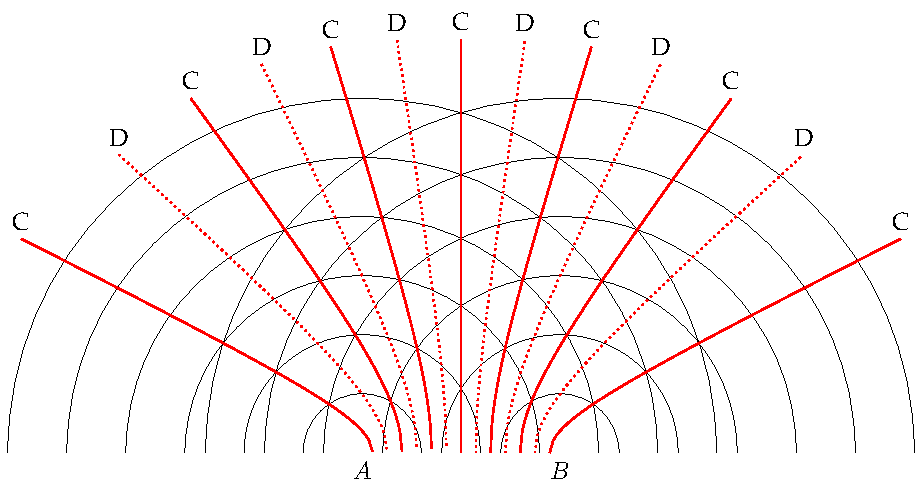
\includegraphics[width=1\textwidth]{interference.pdf}
\caption{constructive (solid lines) and destructive (dashed lines) interference of waves produced from two coherent sources $A$ and $B$}
\end{figure*}
\vspace{1cm}
Regions of constructive interference are often called \emph{maxima}

\begin{compactitem}
	\item[--] points on line C$_0$ are of equal distance to wave sources, i.e., path difference $\Delta L = 0$
	
	so maxima are observed along C$_0$
	
	\item[--] points on C$_1$, C$_2$ and C$_3$ have path difference $\Delta L = \lambda, \, 2\lambda, \, 3\lambda$
	
	so maxima are also formed along C$_1$, C$_2$ and C$_3$
	
	\item[--] equivalently, points on C$_n$ have phase difference $\Delta \phi = n\cdot 2\pi$, where $n=0,1,2,3,\cdots$
\end{compactitem} 

Regions of destructive interference are often called \emph{minima}

\begin{compactitem}
	\item[--] points on D$_1$, D$_2$ and D$_3$ have path difference $\Delta L = \frac{1}{2}\lambda, \, \frac{3}{2}\lambda, \, \frac{5}{2}\lambda$
	
	so maxima are also formed along D$_1$, D$_2$ and D$_3$
	
	\item[--] similarly, points on D$_n$ have phase difference $\Delta \phi = \left( n+\frac{1}{2} \right) \cdot 2\pi$, where $n=1,2,3,\cdots$
\end{compactitem} 

\newpage

Stable interference means regions of maxima/minima remain maxima/minima can be easily seen. This requires \keypoint{coherent} wave sources, which means constant phase difference over time\index{coherence}.

The easiest way to produce coherent waves is to use the the same source, such as

\begin{compactitem}
	\item[--] dippers driven by a common vibrating beam in a ripple tank
	
	\item[--] loudspeakers driven by the same signal generator
 \item[--] a laser beam shone on two slits.
\end{compactitem}

\begin{figure}[ht]
	\centering
	\begin{tikzpicture}[scale=1.2]
	% water in ripple tank
	\draw[cyan!30, fill] (2,-0.3) -- (2,-1.5) -- (-1,-3.5) -- (-5,-3.5) -- (-5,-2.3) -- (-2,-0.3) -- cycle;
	\draw[white, fill, opacity=0.3] (2,0) -- (2,-0.3) -- (-1,-2.3) -- (-5,-2.3) -- (-5,-2) -- (-1, -2) -- cycle;
	% outline for ripple tank
	\draw[gray!40] (-2,-0.3) -- (-2,-1.5) -- (2,-1.5) (-2,-1.5) -- (-5,-3.5);
	\draw[thick] (2,0) -- (2,-1.5) -- (-1,-3.5) -- (-5,-3.5) -- (-5,-2) -- (-2,0) -- cycle;
	\draw[thin, gray] (2,-0.3) -- (-1, -2.3) -- (-5, -2.3) -- (-2,-0.3) -- cycle;
	\draw[thick] (-5,-2) -- (-1, -2) -- (-1, -3.5) (-1, -2) -- (2,0);
	\draw[thick] (-2,0) -- (-2,-0.3);
	% dippers
	\foreach \x in {-0.8,0.9} {
		\draw[thick, fill=orange!40] ({-0.6+\x}, 0.2)  circle (0.4);
		\draw[ultra thick] ({-0.6+\x}, 0.6) -- ({-0.6+\x},1.0);
		\draw[<->] ({-0.6+\x}, -0.25) --++ (0,-0.35);
	}
	\draw[ultra thick] (-1.4, 0.98) -- (0.3, 0.98);
	\draw[ultra thick] (-0.55,1) --++ (0,0.5) --++ (1.2,0.5) node[below right]{to vibrator};
	\draw (0.5, 0.4) --++ (1.2,0.5) node[right]{dipper};
	% ripples
	\draw[gray] (-1.62,-0.4) [out=-75 , in=180] to (-1.45,-0.52) [out=0, in=210] to (-1.0,-0.4);
	\draw[gray] (-1.85,-0.4) [out=-75 , in=180] to (-1.55,-0.65) [out=0, in=210] to (-0.7,-0.4);
	\draw[gray] (-2.08,-0.4) [out=-75 , in=180] to (-1.6,-0.8) [out=0, in=210] to (-0.4,-0.4);
	\draw[gray] (0.08,-0.4) [out=-75 , in=180] to (0.25,-0.52) [out=0, in=210] to (0.7,-0.4);
	\draw[gray] (-0.15,-0.4) [out=-75 , in=180] to (0.15,-0.65) [out=0, in=210] to (1.0,-0.4);
	\draw[gray] (-0.38,-0.4) [out=-75 , in=180] to (0.1,-0.8) [out=0, in=210] to (1.3,-0.4);
	\end{tikzpicture}
	
	\caption{Demonstrating interferece of water waves in a ripple tank}
\end{figure}

Conversely, we do not see interference from beams of light from different lamps or laser sources because light from different sources are usually \emph{incoherent}\footnote{Emission of light is associated with the electronic transitions between energy levels in an atom, which is a completely random process. So in general separate light sources are not coherent.}

This can be overcome by dividing a single beam into several beams using a number of slits. common apparatuses of doing so are the \emph{double-slit} and \emph{diffraction gratings}

\newpage

\subsection{Double-slit interference}\index{double-slit experiement}

Let's take a beam of light being guided through two narrow slits, light waves diffracting through the slits act as coherent wave sources and when they meet on a screen, interference pattern can be seen. Since this experiment is carried out with light, alternating bright and dark fringes are formed. 

This is known as \emph{Thomas Young}'s \keypoint{double-slit experiment}
\footnote[][-4cm]{The nature of light has been argued since the history of human civilisation. It has been long debated whether light is a \emph{wave} or it is made of \emph{particles}. It was until the early 1800s when Thomas Young carried out the famous double-slit experiment that now bears his name, people became certain that light has wavelike properties. We know now of course that it has particle -like properties too. For a detailed review, check out the Wikipedia article: \url{https://en.wikipedia.org/wiki/Light}.}

\colorlet{wall}{blue!30!black}
\colorlet{myblue}{blue!70!black}
\colorlet{myred}{red!70!black}
\colorlet{mydarkred}{red!50!black}
\colorlet{mylightgreen}{green!60!black!70}
\colorlet{mygreen}{green!60!black}
\colorlet{myredgrey}{red!50!black!80}
\colorlet{myshadow}{blue!30!black!90}
\tikzstyle{wave}=[myblue,thick]
\tikzstyle{mydashed}=[black!70,dashed,thin]
\tikzstyle{mymeas}=[{Latex[length=3,width=2]}-{Latex[length=3,width=2]},thin]
\tikzstyle{mysmallarr}=[-{Latex[length=3,width=2]}]

\newcommand\rightAngle[4]{
  \pgfmathanglebetweenpoints{\pgfpointanchor{#2}{center}}{\pgfpointanchor{#3}{center}}
  \coordinate (tmpRA) at ($(#2)+(\pgfmathresult+45:#4)$);
  \draw[white,line width=0.6] ($(#2)!(tmpRA)!(#1)$) -- (tmpRA) -- ($(#2)!(tmpRA)!(#3)$);
  \draw[mydarkred] ($(#2)!(tmpRA)!(#1)$) -- (tmpRA) -- ($(#2)!(tmpRA)!(#3)$);
}
\newcommand\lineend[2]{
  \def\w{0.1} \def\c{30}
  \draw[mygreen] (#1)++(#2:\w) to[out=#2-180-\c,in=#2+\c] (#1)
                               to[out=#2+\c-180,in=#2-\c]++ (#2-180:\w);
}
\def\tick#1#2{\draw[thick] (#1) ++ (#2:0.1) --++ (#2-180:0.2)}

% INTERFERENCE FADING
\begin{tikzfadingfrompicture}[name=interference]
  \def\lambd{0.5} % wavelength
  \foreach \r in {1,...,15}
    \foreach \j in {1,...,25}
       \path [line width=\lambd*\j,draw=transparent!0,opacity=0.04]
          (0,0) circle (\lambd*\r); %(0:\r) arc (0:180:\r);
\end{tikzfadingfrompicture}

\begin{figure*}
	\centering
 \begin{tikzpicture}[
    nodal/.style={mylightgreen,dashed,very thin},
    declare function={
      %xnode(\n,\dn,\lam,\f) = sqrt( (\n^2+(\n+\dn)^2)*\lambd^2/2 - (\n^2-(\n+\dn)^2)^2*\lambd^4/(4*\a^2) - \a^2/4 );
      xnode(\n,\dn,\lam,\f) = \lam/\f*sqrt( \n^2*(\f^2-\dn^2)+\n*\dn*(\f^2-\dn^2)+\dn^2*\f^2/2-(\f^4+\dn^4)/4 );
      ynode(\n,\dn,\lam,\a) = (2*\n*\dn+\dn^2)*\lam/(2*\f);
      intensity(\y,\lam,\a,\L) = cos(180*\a*\y/(2*\lam*sqrt(\L*\L+\y*\y)))^2;
    }
  ]
  
  \def\L{3.8}       % distance between walls
  \def\H{5.4}       % total wall height
  \def\h{2.8}       % plane wave height
  \def\t{0.15}      % wall thickness
  \def\a{1.15}      % slit distance
  \def\d{0.20}      % slit size
  \def\N{21}        % number of waves
  \def\lambd{0.20}  % wavelength
  \def\R{\N*\lambd} % wave radius
  \def\Nlines{3}    % number of nodal lines
  \def\A{1.6}       % amplitude
  %\def\r{0.06}      % point source radius
  %\def\nmax{10}
  \def\nsamples{100}
  \def\ang{62}
  
  \begin{scope}
    \clip (-\t/2,-\H/2) rectangle (\L,\H/2);
    %\clip (-\t/2,0.7*\a) -- (0.6*\L,\H/2) -- (\L,\H/2) --
    %      (\L,-\H/2) -- (0.6*\L,-\H/2) -- (-\t/2,-0.7*\a) -- cycle;
    
    % NODAL LINES
    \draw[nodal]
      (0.08*\N*\lambd,0) -- (1.06*\R,0);
    \coordinate (NP0) at (\L,0);  % to avoid "Dimension too large error"
    \foreach \dn [evaluate={
                   \f=\a/\lambd;
                   \nmin=2.5+0.2*\dn; %0.501*(-\dn+\f)
                   \nmax=10; %(NP0)
                   \c=int(\dn<\f);
                   \y=\L/sqrt((\a/(\lambd*\dn))^2-1);
                 }] in {1,...,\Nlines}{
      \coordinate (NP+\dn) at (\L,\y);  % to avoid "Dimension too large error"
      \coordinate (NP-\dn) at (\L,-\y); % to avoid "Dimension too large error"
      \ifnum\c=1
        \draw[nodal,variable=\n,samples=\nsamples,smooth]
          plot[domain=\nmin:\nmax] ({xnode(\n,\dn,\lambd,\f)},{ynode(\n,\dn,\lambd,\f)})
          -- (NP+\dn);
        \draw[nodal,variable=\n,samples=\nsamples,smooth]
          plot[domain=\nmin:\nmax] ({xnode(\n,\dn,\lambd,\f)},{-ynode(\n,\dn,\lambd,\f)})
          -- (NP-\dn);
      \fi
    }
    
    % WAVES
    \foreach \i [evaluate={\R=\i*\lambd;}] in {1,...,\N}{
      \ifodd\i
        \draw[myblue,line width=0.8] (0,\a/2)++(\ang:\R) arc (\ang:-\ang:\R);
        \draw[myred,line width=0.8] (0,-\a/2)++(\ang:\R) arc (\ang:-\ang:\R);
      \else
        \draw[myblue!80,line width=0.1] (0,\a/2)++(\ang:\R) arc (\ang:-\ang:\R);
        \draw[myred!80,line width=0.1] (0,-\a/2)++(\ang:\R) arc (\ang:-\ang:\R);
      \fi
    }
  \end{scope}
  
  % PLANE WAVES
  \foreach \i [evaluate={\x=-\i*\lambd;}] in {0,...,5}{
    \ifodd\i
      \draw[myblue,line width=0.8] (\x,-\h/2) -- (\x,\h/2);
    \else
      \draw[myblue,line width=0.1] (\x,-\h/2) -- (\x,\h/2);
    \fi
  }
  
  % WALL
  \fill[wall]
    (\t/2,\a/2-\d/2) rectangle (-\t/2,-\a/2+\d/2)
    (\t/2,\a/2+\d/2) rectangle (-\t/2,\H/2)
    (\t/2,-\a/2-\d/2) rectangle (-\t/2,-\H/2)
    (\L,-\H/2) rectangle (\L+\t,\H/2);
  
  % SHADES
  \begin{scope}[shift={(1.08*\L,0)}]
    \def\yz{\L/sqrt((\a/\lambd)^2-1)} % m = +- 1/2
    \def\yZ{\L/sqrt((\a/\lambd/2)^2-1)} % m = +- 1
    \clip (0,-\H/2) rectangle (1.1*\A,\H/2);
    \fill[white] (0,-\H/2) rectangle++ (\A,\H); % to fill seams
    \foreach \i [evaluate={\n=0.5*\i;\yn=\L/sqrt((\a/(2*\lambd*\n))^2-1);
                 }] in {1,...,\Nlines}{
      \ifodd\i % if even
        \fill[myshadow] (0,{-\yn-0.1}) rectangle++ (\A,0.2); % to fill seams
        \fill[myshadow] (0,{ \yn-0.1}) rectangle++ (\A,0.2); % to fill seams
      \fi
    }
    \path[left color=myshadow,right color=myshadow,middle color=white,shading angle={180}]
      (0,{-\yz}) rectangle (\A,{\yz});
    \foreach \i [evaluate={
                  \n=0.5*\i;
                  \m=0.5*(\i+1);
                  \yn=\L/sqrt((\a/(2*\lambd*\n))^2-1);
                  \ym=\L/sqrt((\a/(2*\lambd*\m))^2-1);
                  \dang=mod(\i,2)*180;
                 }] in {1,...,\Nlines}{
      \path[left color=myshadow,right color=white,shading angle={\dang}]
        (0,\yn) rectangle (\A,\ym);
      \path[left color=myshadow,right color=white,shading angle={180+\dang}]
        (0,-\yn) rectangle (\A,-\ym);
    }
  \end{scope}
  
  % INTENSITY
  \begin{scope}[shift={(1.1*\L+1.1*\A,0)}]
    \draw[->,thick] (-0.08*\A,0) -- (1.3*\A,0) node[right=-2] {$\expval{I}$}; % I axis
    \draw[->,thick] (0,-0.52*\H) -- (0,0.54*\H) node[right] {$y$}; % y axis
    \draw[nodal] (NP0) --++ (0.15*\L+2.1*\A,0); % green nodal lines
    \foreach \i [evaluate={\y=\L/sqrt((\a/(\lambd*\i))^2-1)}] in {1,...,\Nlines}{ % green nodal lines
      \draw[nodal] (NP+\i) --++ ({0.15*\L+1.1*\A+\A*intensity(\y,\lambd,\a,\L)},0);
      \draw[nodal] (NP-\i) --++ ({0.15*\L+1.1*\A+\A*intensity(\y,\lambd,\a,\L)},0);
    }
    \draw[myred,thick,variable=\y,samples=\nsamples,smooth,domain=-\H/2:\H/2]
      plot({\A*intensity(\y,\lambd,\a,\L)},\y);
    \foreach \i [evaluate={ % ticks
        \modd=\i; %int(\i);
        \meven=int(\i-1);
        \y=\L/sqrt((\a/(\lambd*\i))^2-1);
                }] in {1,...,\Nlines}{
      \ifodd\i
        \tick{0,-\y}{180} node[right=0,scale=0.85] {$m=-\frac{\modd}{2}$};
        \tick{0,\y}{180} node[right=0,scale=0.85] {$m=+\frac{\modd}{2}$};
      \else
        \tick{0,-\y}{180} node[right=0,scale=0.85] {$m=-\meven$};
        \tick{0,\y}{180} node[right=0,scale=0.85] {$m=+\meven$};
      \fi
    }
  \end{scope}
  
\end{tikzpicture}
	\caption{Young's double-slit interference experiment}
\end{figure*}

When waves from the two slits meet with path difference $\Delta L = 0, \, \lambda, \, 2\lambda, \cdots$, maxima is formed, ie bright fringes are observed.\\
When waves from the two slits meet with path difference $\Delta L = \frac{1}{2}\lambda, \, \frac{3}{2}\lambda, \, \frac{5}{2}\lambda, \cdots$, minima is formed, ie dark fringes are observed.

We can use the geometry of the slit separation, the distance to the screen, and the spacing of the fringes to calculate the wavelength of the light - at least we can if the slit-to-screen distance is much larger than the slit separation, i.e., $D \gg d$.\\

In this case, bright fringes are nearly equally spaced with a separation of: \begin{empheq}[box=\tcbhighmath]{equation*}{x = \frac{\lambda D}{d}}\end{empheq}

where $d$ is separation of the two slits, $D$ is slit-to-screen distance

\begin{figure*}
	\centering
	\begin{tikzpicture}[scale=0.55]
	\coordinate (A) at (0,1); \node[left] at (A) {$A$};
	\coordinate (B) at (0,-1); \node[left] at (B) {$B$};
	\coordinate (O) at (19.5,0);
	\coordinate (P) at (19.5,4);
	% double slit and screen
	\draw[thick] (0,4) -- (0,1.1) (0,0.9) -- (0,-0.9) (0,-1.1) -- (0,-4) node[below]{double slit};
	\draw (P) -- (0,0) node[left]{$M$} -- (O) node[midway,below]{$D$};
	\draw[thick] (19.5,5) -- (P) node[right] {$P$} -- (O) node[right] {$O$} node[midway,left]{$y$} -- (19.5,-5) node[below]{screen};
	% fringes
	\foreach \z in {-4, -2.667, -1.333, 0 , 1.333 ,2.667, 4}{
		\draw[blue,fill] (21.5,\z-0.2) rectangle (22.5,\z+0.2);
		\draw (22.8,\z) -- (23.2,\z);	
	}
	\foreach \z in {-4, -2.667, -1.333, 0 , 1.333 ,2.667}
	\draw[<->] (23,\z+0.03) -- (23,\z+1.273) node[midway,right]{$x$};
	\draw (22,-4.88) node[below] {fringes};
	% paths
	\draw[<->] (-1,1) -- (-1,-1) node[midway,left]{$d$};
	\draw[thick,blue] (A) -- (P) -- (B);
	\draw (0,1) -- (0.4706,-0.8824);
	\draw (0.4706,-0.8824) ++ (-0.05,0.2) -- ++(0.2,0.05) -- ++(0.05,-0.2) node[below]{$H$};
	\draw[ultra thick, red] (B) -- (0.4706,-0.8824);
	% zoom-in view
	\draw (3,0) arc(0:11.3:3); \node[right] at (3,0.32) {$\theta$};
	\draw[densely dotted] (0,0) circle(2);
	\draw[double] (-30:2) -- (10.5,-3);
	\coordinate (A') at (12,-2.5);
	\coordinate (B') at (12,-5.5);
	\draw (12,-1.5) -- (A') node[left] {$A$} -- (B') node[left]{$B$} node[midway,left]{$d$} -- (12,-6);
	\draw[blue] (A') -- ++(30:2.5);
	\draw[blue] (B') -- ++(30:3.6);
	\draw (A') -- ++(-60:2.598);
	\draw[dashed] (A') -- ++(2,0);
	\draw (A') ++ (.8,0) arc(0:30:.8);
	\draw (A') ++ (15:1.1) node{\small$\theta$};
	\draw[dashed] (B') -- ++(2,0);
	\draw (B') ++ (.8,0) arc(0:30:.8);
	\draw (B') ++ (15:1.1) node{\footnotesize$\theta$};
	\draw (A') ++ (0,-.8) arc(270:300:0.8);
	\draw (A') ++ (285:1.1) node{\footnotesize$\theta$};
	\draw[ultra thick,red] (B') -- ++(30:1.5);
	\draw (B') ++(30:1.3) -- ++(120:0.2) -- ++(30:0.2) node[below right]{$H$};
	\draw[red,->] (B') ++(30:.75) to[out=120,in=180] (13,-4.2) to[out=0,in=135] (14.4,-5);
	\draw[red] (14,-5.4) node[right] {\footnotesize{$\Delta L \approx d\sin\theta$}};
	\draw[densely dotted] (10.5,-6.4) rectangle (17.5,-1);
	\end{tikzpicture}
	\label{fringey}
 \caption{Deriving the Young slits formulae.}
\end{figure*}

The derivation of this formulae is one you should know and follows: 
Consider a point $P$ on the screen where a bright fringe is formed (see figure \ref{fringey})

The path difference between the slits must be a whole number of wavelength: $$ \Delta L = \big|PB-PA\big| = n\lambda $$

Because $D \gg d$, paths $PA$ and $PB$ can be considered approximately parallel, so path difference is length of the segment $HB$, then we have: $$\Delta L \approx d\sin\theta$$

In terms of $\theta$, bright fringes are found where: $$ d\sin\theta = n\lambda $$

To convert $\theta$ into the coordinate $y$, we have: $$\tan \theta = \frac{y}{D}$$

Because $\theta$ is very small, the small-angle approximation ($\sin \theta \approx \tan \theta$) can be applied, so positions where the bright fringes show up are: $$ \tcbhighmath{y_n =  n \times \frac{\lambda D}{d}} $$\begin{marginfigure}
\begin{tikzpicture}[scale=.7]
\begin{axis}[
  grid=both,
  xmin=-.1,
  xmax=.6,
  ymin=-.5,
  ymax=1,
  xlabel=$x$,
  ylabel=$y$,
  axis lines=center,
  >=stealth
]
  \addplot[
    domain=-.1:.6,
    blue,
    ultra thick,
    samples=100,
  ] plot[smooth] {sin(deg(x))};
  \addplot[
    domain=-.1:.6,
    red,
    ultra thick,
    samples=100,
  ] plot[smooth] {tan(deg(x))};
\end{axis}
\end{tikzpicture}

\caption{For small values of x, tan(x) [red] and sin(x) [blue] can be considered equal.} 
\end{marginfigure}

Here the coordinate subscript $n$ labels the order of the bright fringes. This shows that the $(n+1)$-th fringe is at a fixed distance from the $n$-th fringe, therefore the separation between neighbouring bright fringes is: $$ {x=\frac{\lambda D}{d}} $$

Aaltering width of slit could cause a change in \emph{brightness} of fringes.

\subsection{Multi-slit interference: diffraction gratings}

Passing light through even more slits also produces nice interference patterns, the \keypoint{diffraction grating} is such an apparatus, with hundreds or thousands of slits per mm\index{diffraction grating}

\begin{figure*}[ht]
	\centering
	\begin{tikzpicture}[xscale=1, yscale=0.84]
	% screen & fringes
	\draw[thick, fill=gray!20] (30:7.5) ++ (-3.2,1) --++ (6.4,0) --++ (0,-2) --++ (-6.4,0) --++ (0,2);
	\foreach \x/\order in {-2.5/2,-1/1,0/0,1/1,2.5/2} \draw[very thick, blue, fill] (30:7.5) ++ (\x, 0) circle (0.05) node[black, above] {{\footnotesize $n=\order$}}-- (30:2);
	% diffraction grating
	\draw[thick,fill=orange!35, opacity=0.75] (30:2) ++ (-0.6,0.6) --++ (1.2,0) --++ (0,-1.2) --++ (-1.2,0) --++ (0,1.2);
	\foreach \x in {0.2,0.16,...,-0.2}
	\draw[ultra thin] (30:2) ++ (-\x-0.01,0.4) --++ (0.02,0) --++ (0,-0.8) --++ (-0.02,0) --++ (0,0.8);
	\draw[very thick, blue] (30:2) -- (0,0);
	% laser source
	\draw[white, fill, opacity=0.75] (-0.6, 0.4) rectangle (0.6,-0.4);
	\draw[thick] (-0.6, 0.4) -- (0.6, 0.4) -- (0.6,-0.4);
	\draw[thick] (-0.6, 0.4) --++ (210:2);
	\draw[thick] (0.6,-0.4) --++ (210:2);
	\draw[thick] (0.6, 0.4) --++ (210:2.4);
	% nodes
	\draw (1.2,-1) node {laser source};
	\draw (30:7.5) ++ (0, 1.1) node[above] {screen};
	\draw (30:2) ++ (0, 0.7) node[above, twoline] {diffraction\\grating};
	\end{tikzpicture}
	\caption{multi-slit interference as light passes through a diffraction grating}
\end{figure*}

Compared to double-slit, maxima produced by diffraction grating are \emph{sharper} and \emph{brighter}, maxima are formed when waves from not two but many slits interfere constructively. The location of each maxima from a diffraction grating is given by: \begin{empheq}[box=\tcbhighmath]{equation*}{d \sin \theta = n\lambda}\end{empheq}

where $d$ is the separation between adjacent slits, and light is incident \emph{normally}.

\begin{figure*}[htp]
	\noindent
	\centering
	\begin{minipage}{0.64\textwidth}
		\centering
		\begin{tikzpicture}[scale=1.15]
		\draw[blue,thick] (-3,0) -- (3,0) node[right] {\textcolor{black}{$n=0$}};
		\foreach \x in {1,2,3}{
			\pgfmathsetmacro{\y}{asin(\x*0.3)}
			\draw[blue,thick] (-\y:3) node[right] {\textcolor{black}{$n=\x$}} -- (0,0) -- (\y:3) node[right] {\textcolor{black}{$n=\x$}};
			\draw[->] ({2-\x*0.5}, 0) arc (0:\y:{2-\x*0.5});
		}
		\draw[fill=gray!50, opacity=0.75] (-0.1,-0.4) rectangle (0.1,0.4);
		\foreach \y in {0.36,0.32,...,-0.36} \draw (-0.1,\y) -- (0.1,\y);
		\node at (8:1.75) {{\footnotesize $\theta_1$}};
		\node at (27:1.25) {{\footnotesize $\theta_2$}};
		\node at (51:0.8) {{\footnotesize $\theta_3$}};
		\end{tikzpicture}
  
  \end{minipage}\hfill
	\begin{minipage}{0.35\textwidth}
		\centering
		\begin{tikzpicture}[scale=1.3]
		\foreach \y in {0,1,2,3,4}
		\draw[ultra thick] (0,\y+0.1) -- (0,\y+0.9);
		\foreach \y in {1,2,3,4}{
			\draw[blue] (0,\y) -- ++(30:2);
			\draw (-0.3,\y) -- (-0.7,\y);
		}
		\foreach \y in {2,3,4}{
			\draw[<->] (-0.5,\y-0.97) -- (-0.5,\y-0.03) node[midway,left]{$d$};
			\draw (0,\y) -- ++(-60:.866);
			\draw[very thick, red] (0,\y-1) -- ++(30:.5);
			\draw[red, decoration={markings,mark=at position 1 with {\arrow[scale=2]{>}}},
			postaction={decorate},dashed] (0,\y-1) -- ++(30:.25) to[out=-45,in=135] (2,1);
			\draw (0,\y-.3) arc(270:300:.3);
			\draw (0,\y) ++ (285:.5) node {\footnotesize$\theta$};
		}
		\node[below] at (2,1) {$\Delta L = d\sin\theta$};
		\end{tikzpicture}
	\end{minipage}
 \caption{Diffraction gratings}
 \end{figure*}

You do not need to be able to reproduce this derivation, but it is offered here in contrast to the above. For constructive interference, path difference between adjacent slits must satisfy: $\Delta L = n\lambda $. Since slits are so close together, we consider the light rays passing through the slits are nearly parallel. Using the same small angle trick as before, we obtain: $d \sin \theta = n\lambda$ - this is known as the \emph{diffraction grating equation}.

Note that the greatest angle through which a beam of light can be diffracted is 90$^\circ$ which puts a constraint on the highest order possible:
\begin{equation*}
n_\tmax = \frac{d\sin\theta_\tmax}{\lambda} < \frac{d \sin 90^\circ}{\lambda} \RA \boxed{n_\tmax < \frac{d}{\lambda}}
\end{equation*}

The value of $\frac{d}{\lambda}$ should be rounded \emph{down} to the nearest whole number to give $n_\tmax$

If white light is passed through diffraction gratings, \emph{dispersion} is observed, this is the cause of the pretty colours seen in a dvd or cd:

\begin{figure*}[!ht]
	\centering
	\begin{tikzpicture}[scale=1.6]
	% background
	\draw[fill=gray!50] (-3.5,-2.7) rectangle (4.2,2.7);
	% zeroth order
	\draw[white,ultra thick] (-3,0) -- (3,0);
	% first and second order
	\foreach \WL/\yanse in {6.4/red, 6.0/orange, 5.6/yellow, 5.2/green, 4.8/blue, 4.4/violet}{
		\pgfmathsetmacro{\ystart}{asin(\WL/18)}
		\pgfmathsetmacro{\yend}{asin((\WL+0.4)/18)}
		\draw[\yanse!80, fill] (0,0) -- (\ystart:3) arc(\ystart:\yend:3) -- cycle;
		\draw[\yanse!80, fill] (0,0) -- (-\ystart:3) arc(-\ystart:-\yend:3) -- cycle;
		\pgfmathsetmacro{\zstart}{asin(\WL/9)}
		\pgfmathsetmacro{\zend}{asin((\WL+0.4)/9)}
		\draw[\yanse!50, fill] (0,0) -- (\zstart:3) arc(\zstart:\zend:3) -- cycle;
		\draw[\yanse!50, fill] (0,0) -- (-\zstart:3) arc(-\zstart:-\zend:3) -- cycle;
	}
	% order labels
	\foreach \t/\nlabel in {0/0, 5.4/1, 10.8/2, -5.4/1, -10.8/2}{
		\pgfmathsetmacro{\y}{asin(\t/18)}
		\node at (\y:3.5) {$n=\nlabel$};
	}
	% diffraction grating
	\foreach \y in {0.36,0.32,...,-0.36} \draw (-0.1,\y) -- (0.1,\y);
	\draw[fill=gray!20, opacity=0.7] (-0.1,-0.4) rectangle (0.1,0.4);
	\end{tikzpicture}
	\caption{dispersion of white light through a diffraction grating}
\end{figure*}

\newpage
Some notes on the peculiarities of this effect:
\begin{compactitem}
	\item[--] At zeroth order, diffraction grating equation $d\sin\theta_0 = 0\cdot\lambda$ is satisfied at $\theta_0 = 0$ for any $\lambda$, so we observe a collection of all colours, i.e., a white central maxima.
	
	\item[--] At first order, $d\sin\theta_1 = 1\cdot\lambda$, maxima for long wavelengths appear at greater angles, so the spectrum spreads into a rainbow band, with red light at outer end and violet closer to the centre.
	
	\item[--] At higher orders, the spectrum would be more spread out as the frequency dependence of diffracted angle becomes more pronounced. The spectra of different orders may even overlap to give complicated combinations.
\end{compactitem}

The diffraction grating is an import device in analysis of light - it is widely used in measurement of wavelength of light and in telecommunications.

\subsection{Diffraction}

A wave has the ability to bend around obstacles or pass through narrow gaps

\begin{ilight}
	When a wave passes through a aperture/slit/gap/hole or encounters an obstacle, it spreads out/around the corners, this is known as \keypoint{diffraction}\index{diffraction} of waves.
\end{ilight}

Diffraction is a general property of all waves. Some examples of diffraction are:

\begin{compactitem}
	\item[--] sound waves can diffract through an open door
	
	so you can hear people in the next room talking, even though you cannot see them
	
	\item[--] light ray can bend when it goes through/around a small hole/small particles
	
	sky appears red at sunset as red light is diffracted most by dust particles in atmosphere
\end{compactitem}

Diffraction is a scale-dependent effect - a wave is diffracted most when its wavelength is close to size of aperture/obstacle. Because a single object is close to an ``infinite gap'', longer wavelengths usually diffracts more around an edge than a wave of shorter wavelength.

\begin{figure*}[htp]
	\centering
	\begin{tikzpicture}[scale=1.25]
	\draw[ultra thick] (0,2.4) -- (0,0.25) (0,-0.25) -- (0,-2.4);
	\foreach \x in {0.25,0.75,1.25,1.75,2.25}{
		\draw[blue,thick] (-\x,-2.4) -- (-\x,2.4);
		\draw[blue,thick] (-65:\x) arc(-65:65:\x);
	}
	\draw[ultra thick] (6,2.4) -- (6,0.8) (6,-0.8) -- (6,-2.4);
	\foreach \x in {0.25,0.75,1.25,1.75,2.25}{
		\draw[blue,thick] (-\x+6,-2.4) -- (-\x+6,2.4);
		\draw[blue,thick] (6,-0.8) ++ (-25:\x) to[out=65,in=270] (6+\x,-0.8-\x/6) -- (6+\x,0.8+\x/6) to[out=90,in=-65] (6+0.9063*\x,0.8+0.4226*\x);
	}
	\end{tikzpicture}
	
	\caption{diffraction of a wave as it passes through an aperture of width that is (a) close to the wavelength, (b) greater than the wavelength}
\end{figure*}

If we go beyond the GCSE understanding of diffraction as above we can we can see that the light passing through a single slit forms a diffraction pattern somewhat different from those formed by double slits or diffraction gratings, which we discuss earlier in the chapter on interference.
\begin{figure*}
    \centering
\begin{tikzpicture}[
    nodal/.style={mylightgreen,dashed,very thin},scale=1.5
  ]
  
  \def\L{3.8}       % distance between walls
  \def\H{5.4}       % total wall height
  \def\h{2.8}       % plane wave height
  \def\t{0.15}      % wall thickness
  \def\a{0.8}       % slit distance
  \def\d{0.20}      % slit size
  \def\N{21}        % number of waves
  \def\dN{1}        % shift radius
  \def\A{1.6}       % amplitude
  \def\lambd{0.20}  % wavelength
  \def\R{\N*\lambd} % wave radius
  \def\Nfringes{2}  % number of nodal lines
  \def\nshades{70}  % number of shades
  \def\nsamples{40}
  \def\ang{40}
  
  % PLANE WAVES
  \foreach \i [evaluate={\xp=-2*(\i-0.5)*\lambd; \xm=-2*(\i-1)*\lambd;}] in {1,...,3}{
    \draw[myblue,line width=0.8] (\xp,-\h/2) -- (\xp,\h/2);
    \draw[myblue,line width=0.1] (\xm,-\h/2) -- (\xm,\h/2);
  }
  
  % WAVES
  \begin{scope}
    \clip (-\t/2,-\H/2) rectangle (\L,\H/2);
    \foreach \i [evaluate={\Rp=2*(\i+\dN)*\lambd; \Rm=2*(\i+\dN+0.5)*\lambd;}] in {1,...,\N}{
      \draw[myblue,line width=0.8] (-2.2*\lambd,0)++(\ang:\Rp) arc (\ang:-\ang:\Rp);
      \draw[myblue!80,line width=0.1] (-2.2*\lambd,0)++(\ang:\Rm) arc (\ang:-\ang:\Rm);
    }
    \foreach \m [evaluate={\ddy=0.1*\m;}] in {1,2,2.7}{ % mask at destructive interference
      \foreach \i [evaluate={\ym=\L/sqrt((\a/(\lambd*\m))^2-1); \dy=0.55*\i/\nshades;}]
        in {1,...,\nshades}{
        \fill[white,opacity=0.045] (0.05,0.005+\ddy) -- (\L,{\dy+\ym}) --++ (0,-2*\dy) -- (0.05,-0.005+\ddy);
        \fill[white,opacity=0.045] (0.05,0.005-\ddy) -- (\L,{\dy-\ym}) --++ (0,-2*\dy) -- (0.05,-0.005-\ddy);
      }
    }
  \end{scope}
  
  % WALL
  \fill[wall]
    (\t/2,\a/2) rectangle (-\t/2,\H/2)
    (\t/2,-\a/2) rectangle (-\t/2,-\H/2)
    (\L,-\H/2) rectangle (\L+\t,\H/2);
  
  % SHADES
  \begin{scope}[shift={(1.08*\L,0)}]
    \clip (0,-\H/2) rectangle (1.1*\A,\H/2);
    \fill[myshadow] (0,-\H/2) rectangle (\A,\H/2); % to fill seams
    \def\yz{\L/sqrt((\a/\lambd)^2-1)} %\L/sqrt((\a/\lambd)^2-1)
    \path [left color=myshadow,right color=myshadow,middle color=white,shading angle={180}]
      (0,{-\yz}) rectangle (\A,{\yz});
    \foreach \i [evaluate={
                  \n=\i;
                  \m=\i+1;
                  \yn=\L/sqrt((\a/(\lambd*\n))^2-1); %\L*\n*\lambd/\a
                  \ym=\L/sqrt((\a/(\lambd*\m))^2-1);
                  \dang=mod(\i,2)*180;
                 }] in {1,...,\Nfringes}{
      \path [left color=myshadow,right color=myshadow,middle color=myshadow!50,shading angle={\dang}]
        (0,\yn) rectangle (\A,\ym);
      \path [left color=myshadow,right color=myshadow,middle color=myshadow!50,shading angle={180+\dang}]
        (0,-\yn) rectangle (\A,-\ym);
    }
  \end{scope}
  
  % INTENSITY
  \begin{scope}[shift={(1.2*\L+1.1*\A,0)}]
    \draw[->,thick] (-0.08*\A,0) -- (1.3*\A,0) node[right=-2] {$\expval{I}$};
    \draw[->,thick] (0,-0.52*\H) -- (0,0.54*\H) node[right] {$y$};
    \draw[myred,thick,variable=\y,samples=\nsamples,smooth,domain=-\H/2:\H/2]
      plot({\A*int_one(\y,\lambd,\a,\L)},\y);
    \foreach \i [evaluate={\y=\L/sqrt((\a/(\lambd*\i))^2-1);}] in {1,...,\Nfringes}{
      \tick{0,-\y}{180} node[right=-1,scale=0.9] {$m=-\i$};
      \tick{0,\y}{180} node[right=-1,scale=0.9] {$m=+\i$};
    }
  \end{scope}
  
\end{tikzpicture}
    
    \caption{Single slit diffraction}
    \label{single slit}
\end{figure*}

Figure \ref{single slit} Shows a single-slit diffraction pattern as we would obseve with eg. a laser. Note that the central maximum is larger than maxima on either side and that the intensity decreases rapidly on either side. In contrast, a diffraction grating produces evenly spaced lines that dim slowly on either side of the center.

\begin{figure*}
\centering
% DIFFRACTION - ONE SLIT - PATH DIFFERENCE close-up
\begin{tikzpicture}[scale=1.5]
  \message{Diffraction, path difference (close-up)^^J}
  
  \def\L{6.15}      % distance between walls
  \def\l{4.0}       % path length
  \def\H{4.3}       % total wall height
  \def\f{0.9}       % fractional height of projection point
  \def\t{0.15}      % wall thickness
  \def\a{2.5}       % slit distance
  \def\ang{26}      % angle
  \coordinate (T) at (0,\a/2);
  \coordinate (B) at (0,-\a/2);
  \coordinate (L) at (0,0);
  \coordinate (R) at (\L,0);
  \coordinate (I) at ({\a/2/tan(\ang)},0);
  
  % LINES
  \draw[mygreen,thick] (T) --++ (\ang:.8*\l) coordinate (PT); %node[midway,below=1,above left=-2] {$r_1$};
  \draw[mygreen,thick] (B) --++ (\ang:\l) coordinate (PB); %node[midway,left=2,below right=-1] {$r_2$};
  \draw[mygreen,thick] (L) --++ (\ang:.9*\l) coordinate (PR);
  \draw[dashed] (T) -- (B);
  \draw[mydarkred,dashed] (T) -- ($(L)!(T)!(PR)$) coordinate (M);
  %\draw[black!60,dashed] (T) --++ (.20*\L,0) coordinate (TR);
  \draw[black!60,dashed] (L) --++ (.6*\L,0) coordinate (LR);
  %\draw[black!60,dashed] (B) --++ (.20*\L,0) coordinate (BR);
  
  % LINE END
  \lineend{PT}{\ang+70}
  \lineend{PR}{\ang+70}
  \lineend{PB}{\ang+70}
  
  % ANGLES
  \draw pic[mysmallarr,"$\theta$",mydarkred,draw=mydarkred,angle radius=20,angle eccentricity=1.3]
    {angle = B--T--M}; %\contour{white}{}
  \draw pic[mysmallarr,"$\theta$",mydarkred,draw=mydarkred,angle radius=24,angle eccentricity=1.2]
    {angle = LR--L--PR};
  \draw pic[mysmallarr,"$\theta$",mydarkred,draw=mydarkred,angle radius=24,angle eccentricity=1.2]
    {angle = LR--I--PB};
  \rightAngle{T}{M}{PR}{0.3}
  
  % MEASURES
  \draw[<->,black] (-2.1*\t,0) --++ (0,\a/2) node[midway,fill=white,inner sep=0.1] {$a/2$};
  \draw[<->,black] (-2.1*\t,0) --++ (0,-\a/2) node[midway,fill=white,inner sep=0.1] {$a/2$};
  \draw[<->,black] ([shift={({\ang-90}:0.1)}]L) -- ([shift={({\ang-90}:0.1)}]M)
    node[midway,left=2,below right=0]{$\frac{a}{2}\!\sin\theta$};
  
  % WALL
  \fill[wall]
    (0,\a/2) rectangle (-\t,\H/2)
    (0,-\a/2) rectangle (-\t,-\H/2);
  
\end{tikzpicture}
\label{singleslitmaths}
\caption{Analysis of single slit diffraction}
 %\forceversofloat
\end{figure*}

The analysis of single-slit diffraction is illustrated in Figure \ref{singleslitmaths} in which the light arrives at the slit, illuminating it uniformly and is in phase across its width. We then consider light propagating onwards from different parts of the same slit. 

Assuming the screen is very far away compared with the size of the slit, rays heading toward a common destination are nearly parallel. When they travel straight ahead, they remain in phase, and we observe a central maximum. However, when rays travel at an angle $\theta$ relative to the original direction of the beam, each ray travels a different distance to a common location, and they can arrive in or out of phase. The ray from the bottom travels a distance of one wavelength farther than the ray from the top. Thus, a ray from the center travels a distance $\lambda/2$ less than the one at the bottom edge of the slit, arrives out of phase, and interferes destructively. A ray from slightly above the center and one from slightly above the bottom also cancel one another. In fact, each ray from the slit interferes destructively with another ray. In other words, a pair-wise cancellation of all rays results in a dark minimum in intensity at this angle. By symmetry, another minimum occurs at the same angle to the right of the incident direction (toward the bottom of the figure) of the light.

% \begin{tikzpicture}
%   \message{Diffraction, path difference^^J}
  
%   \def\L{5.9}       % distance between walls
%   \def\H{4.3}       % total wall height
%   \def\f{0.95}      % fractional height of projection point
%   \def\ang{atan((\f*\H+\a/2)/\L/2)} % theta
%   \def\t{0.15}      % wall thickness
%   \def\a{2.5}       % slit distance
%   \coordinate (T) at (0,\a/2);
%   \coordinate (B) at (0,-\a/2);
%   \coordinate (L) at (0,0);
%   \coordinate (R) at (\L,0);
%   \coordinate (P) at (\L,\f*\H/2);
%   \coordinate (M) at ($(L)!(T)!(P)$);
  
%   % LINES
%   \draw[mygreen,thick] (T) -- (P); %node[midway,above=-1] {$r_1$};
%   \draw[mygreen,thick] (B) -- (P); %node[midway,below=3,right=6] {$r_2$}; %right=6,below right=-4
%   \draw[mygreen,thick] (L) -- (P);
%   \draw[dashed] (T) -- (B);
%   \draw[dashed,black!60] (L) -- (R);
%   \draw[mydarkred,dashed] (M) -- (T);
  
%   % ANGLES
%   \draw pic[mysmallarr,"$\theta'$",mydarkred,draw=mydarkred,angle radius=25,angle eccentricity=1.2]
%     {angle = B--T--M};
%   \draw pic[mysmallarr,"$\theta$",mydarkred,draw=mydarkred,angle radius=31,angle eccentricity=1.14]
%     {angle = R--L--P};
%   \rightAngle{T}{M}{P}{0.3}
  
%   % MEASURES
%   \draw[<->,black] (0,-0.47*\H) --++ (\L,0) node[midway,fill=white,inner sep=1] {$L$};
%   \draw[<->,black] (-2.1*\t,0) --++ (0,\a/2) node[midway,fill=white,inner sep=0.1] {$a/2$};
%   \draw[<->,black] (-2.1*\t,0) --++ (0,-\a/2) node[midway,fill=white,inner sep=0.1] {$a/2$};
%   \draw[<->,black] ([shift={({\ang-100}:0.1)}]L) -- ([shift={({\ang-100}:0.1)}]M)
%     node[midway,left=3,below right=-2]{$\frac{a}{2}\sin\theta'$};
%   \draw[<->,black] ([shift={(2.1*\t,0)}]P) -- ([shift={(2.1*\t,0)}]R)
%     node[midway,fill=white,inner sep=1]{$y$};
  
%   % WALL
%   \fill[wall]
%     (0,\a/2) rectangle (-\t,\H/2)
%     (0,-\a/2) rectangle (-\t,-\H/2)
%     (\L,-\H/2) rectangle (\L+\t,\H/2);
%   \fill[mygreen!80!black] (P) circle (0.3*\t) node[right=1,above left=-1] {P};
  
% \end{tikzpicture}

As seen in the figure, the difference in path length for rays from either side of the slit is  $a \sin{\theta}$  and we see that a destructive minimum is obtained when this distance is an integral multiple of the wavelength.

Thus, to obtain destructive interference for a single slit,

$$ a \sin{\theta} = m \lambda$$ 
Where:
m is the order of the minimum.\\
a is the slit width,\\
$\lambda$  is the light’s wavelength,\\
$\theta$  is the angle relative to the original direction of the light\\

% \begin{figure}
%     \centering
%     % TWO SPLIT: interference x diffraction
% \begin{tikzpicture}
%  \def\A{3.5}
%  \def\d{3.4}     % slit distance
%  \def\a{0.9}     % slit size
%  \def\lambd{0.2} % wavelength
%  \def\k{15}      % x -> theta
%  \def\xmax{4.6}
%  \def\ymax{\A}
%  \def\N{4}
%  \def\D{2.3*\xmax}
%  \def\L{4.0}
%  \def\nsamples{80}
 
%  \draw[->,thick,black] (-1.05*\xmax,0) -- (1.1*\xmax,0) node[below] {$\theta$};
%  \draw[->,thick,black] (0,-0.1*\A) -- (0,1.12*\A);
%  \draw[wave,variable=\t,samples=\nsamples,smooth,domain=-\xmax:\xmax]
%     plot(\t,{\A*int_one_ang(\k*\t,\lambd,\a)});
 
%  \foreach \i [evaluate={\t=asin(\i*\lambd/\a)/\k;}] in {1,...,\N}{
%     \tick{-\t,0}{90} node[below=-1,scale=0.7] {$m=-\i$};
%     \tick{\t,0}{90} node[below=-1,scale=0.7] {$m=+\i$};
%  }
 
% \end{tikzpicture}
%     \caption{Caption}
%     \label{fig:enter-label}
% \end{figure}

\newpage

\subsection{Stationary waves}

\subsection{Formation of stationary waves}

Stationary waves are often formed when a travelling wave is \emph{reflected}. Forward-moving wave and backward-moving reflected wave combine to form stationary wave.

\begin{ilight}
	When two waves of same frequency and same speed travel in opposite directions and meet together, they superpose to form stable regions of constructive and destructive interference, this forms a \keypoint{stationary wave}, also known as a \keypoint{standing wave}\index{stationary wave}
\end{ilight}

\begin{figure*}[htp]
	\centering
	\noindent\begin{minipage}{0.25\linewidth}
		\centering
		\begin{tikzpicture}[scale=0.5]
		\foreach \y in {0, -3.5, -7.5}
		\draw[thin, dashed] (-pi, \y) -- (pi, \y);
		\draw [thick,blue,domain=-pi:pi,samples=24,smooth,variable=\x] plot (\x,{sin(\x r)});
		\draw[->,blue] (-0.5,1.5) -- (0.5,1.5);
		\draw [thick,Green,domain=-pi:pi,samples=24,smooth,variable=\x] plot (\x,{sin(-\x r)-3.5});
		\draw[<-,Green] (-0.5,1.5-3.5) -- (0.5,1.5-3.5);
		\draw [very thick,red,domain=-pi:pi,samples=5,smooth,variable=\x] plot (\x,{-7.5});
		\node at (0,-11) {$t=0$};
		\node[white] at (2,-11) {$\frac{1}{1}$};
		\end{tikzpicture}
	\end{minipage}\hfil
	\begin{minipage}{0.25\linewidth}
		\centering
		\begin{tikzpicture}[scale=0.5]
		\foreach \y in {0, -3.5, -7.5}
		\draw[thin, dashed] (-pi, \y) -- (pi, \y);
		\draw [thick,blue,domain=-pi:pi,samples=24,smooth,variable=\x] plot (\x,{-cos(\x r)});
		\draw[->,blue] (-0.5,1.5) -- (0.5,1.5);
		\draw [thick,Green,domain=-pi:pi,samples=24,smooth,variable=\x] plot (\x,{-cos(\x r)-3.5});
		\draw[<-,Green] (-0.5,1.5-3.5) -- (0.5,1.5-3.5);
		\draw [very thick,red,domain=-pi:pi,samples=24,smooth,variable=\x] plot (\x,{-2*cos(\x r)-7.5});
		\node at (0,-11) {$t=\frac{T}{4}$};
		\end{tikzpicture}
	\end{minipage}\hfil
	\begin{minipage}{0.25\linewidth}
		\centering
		\begin{tikzpicture}[scale=0.5]
		\foreach \y in {0, -3.5, -7.5}
		\draw[thin, dashed] (-pi, \y) -- (pi, \y);
		\draw [thick,blue,domain=-pi:pi,samples=24,smooth,variable=\x] plot (\x,{-sin(\x r)});
		\draw[->,blue] (-0.5,1.5) -- (0.5,1.5);
		\draw [thick,Green,domain=-pi:pi,samples=24,smooth,variable=\x] plot (\x,{-sin(-\x r)-3.5});
		\draw[<-,Green] (-0.5,1.5-3.5) -- (0.5,1.5-3.5);
		\draw [very thick,red,domain=-pi:pi,samples=5,smooth,variable=\x] plot (\x,{-7.5});
		\node at (0,-11) {$t=\frac{T}{2}$};
		\end{tikzpicture}
	\end{minipage}\hfil
	\begin{minipage}{0.25\linewidth}
		\centering
		\begin{tikzpicture}[scale=0.5]
		\foreach \y in {0, -3.5, -7.5}
		\draw[thin, dashed] (-pi, \y) -- (pi, \y);
		\draw [thick,blue,domain=-pi:pi,samples=24,smooth,variable=\x] plot (\x,{cos(\x r)});
		\draw[->,blue] (-0.5,1.5) -- (0.5,1.5);
		\draw [thick,Green,domain=-pi:pi,samples=24,smooth,variable=\x] plot (\x,{cos(\x r)-3.5});
		\draw[<-,Green] (-0.5,1.5-3.5) -- (0.5,1.5-3.5);
		\draw [very thick,red,domain=-pi:pi,samples=24,smooth,variable=\x] plot (\x,{2*cos(\x r)-7.5});
		\node at (0,-11) {$t=\frac{3T}{4}$};
		\end{tikzpicture}
	\end{minipage}
		\caption{The formation of a stationary wave (red) due to the superposition of one wave travelling to the right (blue) and another wave travelling to the left (green)}
\end{figure*}

from this one can visualise how the pattern of a stationary wave varies with time (see Figure \ref{fig:statwave}. There are points in the wave where destructive interference always occurs, these points are called \keypoint{nodes}, which have zero amplitudes. \index{node}

The points oscillating with the greatest amplitudes are called \keypoint{anti-nodes}. \index{anti-node} Points other than nodes and anti-nodes oscillate with different amplitudes. 

\begin{figure*}[htp]
	\centering
	\begin{tikzpicture}[scale=0.7]
	\foreach \amp in {-2,-1,1,2}
	\draw [thick,red,domain=-3*pi:3*pi,samples=60,smooth,variable=\x] plot (\x,{\amp*sin(\x r)});
	\draw [thick,blue] (-3*pi,0) -- (3*pi,0);
	\foreach \idx in {-1,0,1}{
		\draw[<->] (\idx*2*pi-pi+0.03,-2.5) -- ++(2*pi-0.06,0) node[midway,above]{$\lambda$};
		\draw (\idx*2*pi-pi,-2.8) -- ++(0,0.6) ++(2*pi,0) -- ++(0,-0.6);
	}
	\foreach \n in {-3,-2,...,3} \node at (\n*pi,0.7) {N};
	\foreach \a in {-2.5,-1.5,...,2.5} \node at (\a*pi,2.25) {A};
	\end{tikzpicture}
	\caption{variation of a stationary wave pattern with time}
 \label{fig:statwave}
\end{figure*}
The distance between two adjacent nodes is half of one wavelength. This allows us to say:: \begin{empheq}[box=\tcbhighmath]{equation*}{\text{the wavelength }\lambda = 2 \times \text{node-to-node distance}}\end{empheq}

\subsection{Stationary wave pattern \& boundary conditions}

Patterns of stationary waves depend heavily on the boundary conditions
The end can be \emph{fixed}, also called a \emph{closed} end, to form a \emph{node} - such as with a wave on a string.

The end can also be \emph{free} to oscillate, known as an \emph{open} end, to form \emph{an anti-node} - such as you might find in a flute.

\subsection*{Stationary wave between two fixed ends}

With both ends fixed, the two ends are both nodes, three patterns with the longest wavelengths and lowest frequencies are shown:

\begin{figure*}[htp]
	\centering
	\noindent\begin{minipage}{0.3\linewidth}
		\centering
		\begin{tikzpicture}[scale=0.7]
		\draw [thick,blue,domain=-pi:pi,samples=24,smooth,variable=\x] plot (\x,{cos(\x/2 r)});
		\draw [thick,dashed,blue,domain=-pi:pi,samples=24,smooth,variable=\x] plot (\x,{-cos(\x/2 r)});
		\node at (0,-2) {fundamental mode};
		\end{tikzpicture}
	\end{minipage}\hfil
	\begin{minipage}{0.3\linewidth}
		\centering
		\begin{tikzpicture}[scale=0.7]
		\draw [thick,blue,domain=-pi:pi,samples=24,smooth,variable=\x] plot (\x,{sin(\x r)});
		\draw [thick,dashed,blue,domain=-pi:pi,samples=24,smooth,variable=\x] plot (\x,{-sin(\x r)});
		\node at (0,-2) {2nd harmonic};
		\end{tikzpicture}
	\end{minipage}\hfil
	\begin{minipage}{0.3\linewidth}
		\centering
		\begin{tikzpicture}[scale=0.7]
		\draw [thick,blue,domain=-pi:pi,samples=24,smooth,variable=\x] plot (\x,{cos(3*\x/2 r)});
		\draw [thick,dashed,blue,domain=-pi:pi,samples=24,smooth,variable=\x] plot (\x,{-cos(3*\x/2 r)});
		\node at (0,-2) {3rd harmonic};
		\end{tikzpicture}
	\end{minipage}\hfil
\end{figure*}

The longest-wavelength mode is called the \emph{fundamental mode}, it also has lowest frequency. Modes with higher frequencies are usually referred to as \emph{excited modes}, or \emph{harmonics}\footnote{These modes are closely related to the notes played on musical instruments.}
in many texts different modes are labelled as 1st, 2nd, 3rd \emph{harmonics}, etc.

If two ends are separated by a distance of $L$, then wavelengths for different modes are:
\begin{equation*}
\lambda_1 = 2L \qquad \lambda_2 = L \qquad \lambda_3 = \frac{2L}{3} \qquad \cdots \qquad \lambda_n = \frac{2L}{n}
\end{equation*}

Making comparison with the fundamental wavelength $\lambda_1$ $\lambda_1$, we have
\begin{equation*}
\lambda_2 = \frac{\lambda_1}{2} \qquad \lambda_3 = \frac{\lambda_1}{3} \qquad \cdots \qquad \lambda_n = \frac{\lambda_1}{n}
\end{equation*}

Since wave speed remains constant as wave travels through the same medium, the frequency of each mode is inversely proportional to its wavelength, hence,  
\begin{equation*}
f_2 = 2f_1 \qquad f_3 = 3f_1 \qquad \cdots \qquad f_n=n f_1
\end{equation*}

\begin{figure*}[ht]
	\centering
	\begin{tikzpicture}[scale=1.1]
	\draw [thick,domain=0:10,samples=90,smooth] plot (\x,{.6*sin(\x*90)});
	\draw [thick,domain=0:10,samples=90,smooth] plot (\x,{-.6*sin(\x*90)});
	\draw[fill] (0,0) circle (0.1);
	\draw[fill] (10,0) circle (0.1);
	\draw[thick] (10,-1) -- (10,1);
	\foreach \y in {0.9,0.6,...,-0.7} \draw (10,\y) --++ (0.2,-0.2);
	\draw (-0.03, 0) rectangle (0.03, -1);
	\draw[thick] (-.8, -1) rectangle (.8,-2);
	\node at (0,-1.5) {oscillator};
	\node[twoline, right] at (10.2, 0) {fixed\\point};
	\end{tikzpicture}
	\caption{Melde's experiment: demonstration of stationary waves on a tense string}
\end{figure*}

\footnote{The speed $v$ of a progressive wave travelling along a string of length $L$ and mass $m$ can be given by the equation: $v = \sqrt{\frac{TL}{m}}$, where $T$ is the tension in the string.} for same frequency, so $\lambda$ increases)

\subsection*{Stationary wave between one fixed end and one open end}

In this case, we have a node at one end and an anti-node at the other end, again we give the three patterns with the longest wavelengths and lowest frequencies.

\begin{figure*}[htp]
	\centering
	\noindent\begin{minipage}{0.3\linewidth}
		\centering
		\begin{tikzpicture}[scale=0.7]
		\draw [thick,blue,domain=0:2*pi,samples=24,smooth,variable=\x] plot (\x,{sin(\x/4 r)});
		\draw [thick,dashed,blue,domain=0:2*pi,samples=24,smooth,variable=\x] plot (\x,{-sin(\x/4 r)});
		\node at (pi,-2) {fundamental mode};
		\end{tikzpicture}
	\end{minipage}\hfil
	\begin{minipage}{0.3\linewidth}
		\centering
		\begin{tikzpicture}[scale=0.7]
		\draw [thick,blue,domain=0:2*pi,samples=24,smooth,variable=\x] plot (\x,{sin(3*\x/4 r)});
		\draw [thick,dashed,blue,domain=0:2*pi,samples=24,smooth,variable=\x] plot (\x,{-sin(3*\x/4 r)});
		\node at (pi,-2) {2nd harmonic};
		\end{tikzpicture}
	\end{minipage}\hfil
	\begin{minipage}{0.3\linewidth}
		\centering
		\begin{tikzpicture}[scale=0.7]
		\draw [thick,blue,domain=0:2*pi,samples=24,smooth,variable=\x] plot (\x,{sin(5*\x/4 r)});
		\draw [thick,dashed,blue,domain=0:2*pi,samples=24,smooth,variable=\x] plot (\x,{-sin(5*\x/4 r)});
		\node at (pi,-2) {3rd harmonic};
		\end{tikzpicture}
	\end{minipage}\hfil
%	\caption{The three lowest frequency modes of wave patterns formed between one fixed end and one open end}
\end{figure*}

\cmt longest-wavelength/lowest-frequency mode is also called the \emph{fundamental mode}

excited modes are called \emph{harmonics} as before

\cmt wavelengths for allowed patterns under the boundary conditions are
\begin{equation*}
\lambda_1 = 4L \qquad \lambda_2 = \frac{4L}{3} \qquad \lambda_3 = \frac{4L}{5} \qquad \cdots \qquad \lambda_n = \frac{4L}{2n-1}
\end{equation*}

comparing with the fundamental wavelength $\lambda_1$, we find
\begin{equation*}
\lambda_2 = \frac{\lambda_1}{3} \qquad \lambda_3 = \frac{\lambda_1}{5} \qquad \cdots \qquad \lambda_n = \frac{\lambda_1}{2n-1}
\end{equation*}

again the wave speed should be the same for all modes, so the allowed frequencies are
\begin{equation*}
f_2 = 3f_1 \qquad f_3 = 5f_1 \qquad \cdots \qquad f_n=(2n-1) f_1
\end{equation*}

\begin{marginfigure}
	\vspace*{-5pt}
	\centering
	\begin{tikzpicture}[xscale=0.64, yscale=0.85]
	\draw[<->] (9,1.8) -- (0,1.8) node[midway,above]{30 cm}; 
	\draw[very thick] (9,1) -- (0,1) -- (0,-1) -- (9,-1);
	\draw [thick,domain=0:9,samples=90,smooth] plot (\x,{0.95*sin(\x*30)});
	\draw [thick,domain=0:9,samples=90,smooth] plot (\x,{-0.95*sin(\x*30)});
	\end{tikzpicture}
	\vspace*{-16pt}
\end{marginfigure}

	

\begin{marginfigure}
	\vspace*{-8pt}
	\centering
	\begin{tikzpicture}[scale=1.5]
	\draw[cyan!40, fill] (-0.5,0) rectangle (0.5, 2.5);
	\draw[cyan!40, fill] (-0.8,0.3) rectangle (-0.5, 0.6);
	\draw[thick] (-0.8, 0.3) -- (-0.5, 0.3) -- (-0.5, 0) -- (0.5, 0) -- (0.5, 4); 
	\draw[thick] (-0.8, 0.6) -- (-0.5, 0.6) -- (-0.5, 4); 
	\draw[ultra thick] (-0.4, 4.5) -- (0.3, 4.5) arc(90:-90:0.1) -- (-0.4, 4.3);
	\draw[ultra thick] (0.4, 4.4) --++ (0.4,0);
	\draw (0.6, 4.5) --++ (0.4, 0.3) node[right, twoline]{tuning\\fork};
	\draw (0.3, 2) --++ (0.6, 0.4) node[right]{water};
	\draw[thick,->] (-0.9, 0.45) --++ (-0.4,0);
	\draw[very thick] (-1,0) -- (1,0);
	\end{tikzpicture}
	\vspace*{10pt}
\end{marginfigure}

\subsection*{Stationary wave between two open ends}

This is left as an exercise for the reader to prove:

You should verify that the allowed wavelengths are: $\lambda = 2L, \, L, \,\frac{2}{3}L, \cdots, \frac{2L}{n}, \cdots$

Frequencies of the fundamental and excited modes go as $f = f_1, \, 2f_1, \, 3f_1, \cdots, nf_1 \cdots$

\subsection{Measurement of speed of sound with stationary waves}
The required practical version of this is covered in Example \ref{recpracwave}, however there is a version that often appears in exam questions as follows;

\begin{figure}[ht]
	\centering
	\begin{circuitikz}
		% loudspeaker
		\draw (-0.6,0.55) to[loudspeaker, name=L] (-0.6,-0.55);
%		\node [waves, scale=0.7, right] at(L.north) {};
		\node[above] at (-0.6,0.65) {loudspeaker};
		% microphone
		\draw[thick] (5.22,0) rectangle (5.38,-0.8);
		\draw[thick, fill=white] (5.3,0) circle (0.2);
		\draw[thick] (5.3, -0.8) [out=-90, in=60] to (3.5,-2); 
		\node[above] at (5.3, 0.3) {microphone};
		\draw[thick, ->] (5.6,0) --++ (0.4,0);
		\draw[thick, ->] (5.0,0) --++ (-0.4,0);
		% oscilloscope
		\draw[thick, rounded corners] (1.9,-2) rectangle (5,-4);
		\draw[rounded corners] (2, -2.1) rectangle (4, -3.9);
		\foreach \y in {-2.4, -3, -3.6} {
			\draw[thick] (4.5, \y) circle (0.2);
		}
		\foreach \x in {2.2, 2.4, ..., 3.8} \draw[very thin, gray!40] (\x, -2.1) -- (\x, -3.9);
		\foreach \y in {-2.3, -2.5, ..., -3.7} \draw[very thin, gray!40] (2, \y) -- (4, \y);
		\draw [thick,Green, domain=2:4,samples=80,smooth] plot (\x,{0.65*sin((\x-2.7)*540) - 3});
		\node[below] at (3.5, -4.1) {oscilloscope};
		% metal plate
		\draw[thick, fill=gray!20] (9,0) ++ (-0.4,1) --++ (0.8,-0.5) --++ (0,-2) --++ (-0.8,0.5) --++ (0,2);
		\node[above] at (9, 1) {metal plate};
		% wave pattern
		\draw [gray, dashed, domain=0:9,samples=80,smooth] plot (\x,{0.3*sin(\x*80)});
		\draw [gray, dashed, domain=0:9,samples=80,smooth] plot (\x,{-0.3*sin(\x*80)});
	\end{circuitikz}
	\caption{arrangement of apparatuses for setting up a stationary sound wave}
\end{figure}

\cmt To set up a stationary sound wave, we need two travelling waves in opposite directions, this sound wave can be produced by a \emph{loudspeaker} (coupled to a \emph{signal generator}). The forward-travelling wave is reflected at a \emph{metal plate} and the reflected wave superposes with wave from loudspeaker to give a stationary wave.
The wave intensity at any point can be detected by a \emph{microphone} and observed on an \emph{oscilloscope}. To verify whether stationary wave is formed, we check whether nodes are formed - the positions of the metal plate and the microphone are adjusted carefully and if there exists a location where no signal is detected, this means microphone is at a node and a stationary wave has been formed between loudspeaker and reflector.
To then find wavelength of sound wave, we slowly move microphone to the next node, the wavelength of sound wave: $\lambda = 2\times \text{distance between neighbouring nodes}$

To find frequency of sound wave, we move microphone to anywhere that is not a node, from time base of the oscilloscope, we can work out period $T$ of the wave. Frequency is then given by the formula: $f=\frac{1}{T}$.

Finally,  speed of the sound wave\footnote{We should bear in mind that stationary waves do not propagate through space, so rigorously speaking, it is incorrect to say the speed of a stationary way. The wave speed calculated in this way refers to the speed of either of the two travelling waves that give rise to the stationary wave through superposition.} can be calculated: $v=\lambda f$

\subsection{Stationary waves \& progressive waves}

There are quite a few differences between a stationary wave and a progressive wave:

A progressive wave can transfer energy from one place to another but for stationary waves, vibrational energy is not transferred due to existence of nodes. 

In a stationary wave, all part have the same amplitude. Different points in general have different amplitudes over a stationary wave. Nodes have zero amplitude, anti-nodes have greatest amplitudes. Other points have various amplitudes depending on their positions.

In a progressive wave the displacements of each point at a particular moment can be all different, but the largest displacements they can reach are the same (if no loss of energy). This means that the phase difference between any two points in a progressive wave can take any value and different points reach their peaks at different times for a progressive wave so $\Delta \phi$ can be anything from 0 to $2\pi$ (or anything from 0 to $360^\circ$).

Phase difference between any two points in a stationary wave however, is either 0 or $\pi$ (or $180^\circ$). For points between adjacent nodes, they all reach their highest at same time despite differences in amplitudes, these points are all in phase, so $\Delta \phi=0$.
For points separated by one node, they are anti-phase, because when one is at its peak, the other is at its trough, so $\Delta \phi = \pi$ (or $180^\circ$)

	
\section{End-of-chapter questions}

\subsection*{Principle of superposition}

\subsection*{Double-slit experiment}

\newpage

\subsection*{Diffraction gratings}

\subsection*{Stationary waves}

\begin{figure}[ht]
	\centering
	\begin{circuitikz}
		% loudspeaker
		\draw (-0.8,0.55) to[loudspeaker, name=L] (-0.8,-0.55);
		% pipe
		\draw[thick] (0,-0.75) --++ (10,0) --++ (0,1.5) --++ (-10,0);
		\draw [gray!50, fill, domain=0:10,samples=80,smooth] plot (\x,{-0.1*cos(\x*180)-0.6}) --++ (0,-0.05) --++ (-10,0) -- cycle;
		% labels
		\draw (8,0.8) --++ (0.6,0.5) node[above]{tube};
		\draw (-0.75,0.7) --++ (0.2,0.5) node[above]{loudspeaker};
		\draw (3,-0.6) --++ (0.4,1.9) node[above]{dust heap};
		\draw[dashed] (3,-0.8) --++ (0,-0.8);
		\draw[dashed] (9,-0.8) --++ (0,-0.8);
		\draw[<->] (3, -1.4) -- (9,-1.4) node[midway, above]{30 cm};
	\end{circuitikz}
\end{figure}
\newpage

\begin{figure}[ht]
	\centering
	\begin{tikzpicture}[scale=1.25]
	\draw [thick, domain=0:8,samples=80,smooth] plot (\x,{0.8*sin(\x*90)});
	\draw[fill] (0,0) circle (0.05) node[left]{$X$};
	\draw[fill] (8,0) circle (0.05) node[right]{$Y$};
	\draw (5.5, 0.75*0.8) --++ (0.5,0.5) node[right]{elastic cord};
	\draw[fill, red] (0.5, {0.8*sin(45)}) circle(0.05) node[above left, black]{$A$};
	\draw[fill, red] (3, -0.8) circle(0.05) node[below, black]{$B$};
	\end{tikzpicture}
\end{figure}

\cleardoublepage

% ===== Chapter: cosmology =====
\chapter{Cosmology}

\section{Stephan's law}
An objects luminosity depends on two factors:
Its surface temperature
Its surface area
The relationship between these is known as Stefan's Law or the Stefan-Boltzmann Law, which states:
The total energy emitted by a black body per unit area per second is proportional to the fourth power of the absolute temperature of the body

So Stefan's Law shows that the luminosity of a star is directly proportional:
\begin{itemize}
    \item To its radius $L \propto r^2$
    \item To its surface area $L \propto 4 \pi r^2$
    \item To its surface absolute temperature $L \propto T^4$
\end{itemize}

Stefan's Law equation is given by:
\begin{equation*}
    L = 4 \pi r2\sigma T^{4}
\end{equation*}

Where:
L = luminosity of the star (W)\\
r = radius of the star\\
$\sigma$ = the Stefan-Boltzmann constant\\
T = surface temperature of the star (K)\\
The surface area of a star (or other spherical object) can be calculated using: $A = 4\pi r^2$\\
Where r = radius of the star

\section{Wein's law}

\subsection{Black Body Radiator}
An ideal black body radiator is one that absorbs and emits all wavelengths.\\
A black body is a theoretical object, however, stars are the best approximation there is.\\
The radiation emitted from a black body has a characteristic spectrum that is determined by the temperature alone.
% CUSTOM COLORS
% See https://tikz.net/blackbody_color/
\definecolor{1000K}{rgb}{1,0.0337,0}
\definecolor{2000K}{rgb}{1,0.2647,0.0033}
\definecolor{3000K}{rgb}{1,0.4870,0.1411}
\definecolor{4000K}{rgb}{1,0.6636,0.3583}
\definecolor{5000K}{rgb}{1,0.7992,0.6045}
\definecolor{6000K}{rgb}{1,0.9019,0.8473}
\definecolor{8000K}{rgb}{0.7874,0.8187,1}
\definecolor{10000K}{rgb}{0.6268,0.7039,1}
\pgfdeclareverticalshading{rainbow}{100bp}{
  color(0bp)=(red); color(25bp)=(red); color(35bp)=(yellow);
  color(45bp)=(green); color(55bp)=(cyan); color(65bp)=(blue);
  color(75bp)=(violet); color(100bp)=(violet)
}
\colorlet{myred}{red!70!black}
\colorlet{mygreen}{green!70!black}
\colorlet{mydarkgreen}{green!55!black}
\pgfmathdeclarefunction{planck}{2}{%
  \pgfmathparse{1.191042972e26/(#1^5)/(exp(0.01439e9/(#1*#2))-1)}%
}
\pgfmathdeclarefunction{rayleighjeans}{2}{%
  \pgfmathparse{8.278160269e18*#2/(#1^4)}%
}
\pgfmathdeclarefunction{wien}{2}{%
  \pgfmathparse{1.191042972e26/(#1^5)*exp(-0.01439e9/(#1*#2))}%
}
\pgfmathdeclarefunction{lampeak}{1}{% % Wien's displacement law
  \pgfmathparse{2.898e6/#1}%
}
\begin{figure*}

\begin{tikzpicture}[scale=1.5]
  \def\N{60}
  \def\xmax{3100}
  \def\ymax{1.36e10}
  \def\tick#1#2{\draw[thick] (#1+.01*\ymax) -- (#1-.01*\ymax) node[below=-.5pt,scale=0.75] {#2};}
  \begin{axis}[
      every axis plot/.style={
        mark=none,samples=\N,domain=5:\xmax,smooth},
      xmin=(-.05*\xmax), xmax=(1.05*\xmax),
      ymin=(-.08*\ymax), ymax=(1.08*\ymax),
      restrict y to domain=0:\ymax,
      axis lines=middle,
      axis line style=thick,
      %enlargelimits=upper, % extend the axes a bit to the right and top
      tick style={black,thick},
      ticklabel style={scale=0.8},
      %xtick style={draw=none},xticklabels=none,
      max space between ticks=26,
      xlabel={Wavelength $\lambda$ [nm]},
      ylabel={Power $P$ [kW/sr\,m$^2$\,nm]},
      xlabel style={at={(rel axis cs:0.5,0)},below=-1pt,font=\small},
      ylabel style={at={(rel axis cs:-0.11,0.5)},rotate=90},
      width=9cm, height=7cm,
      %clip=false
      tick scale binop=\times,
      every y tick scale label/.style={at={(rel axis cs:0,1)},anchor=south}]
    ]
    
    % RAINBOW
    \shade[shading=rainbow,shading angle=90,opacity=0.5] (380,0) rectangle (740,\ymax);
    \node[above=-1pt,scale=0.8] at (200,\ymax) {\strut UV}; % 10 - 400 nm
    \node[above=-1pt,scale=0.8] at (570,\ymax) {\strut optical}; % 380 - 740 nm
    \node[above=-1pt,scale=0.8] at (920,\ymax) {\strut IR}; % 740 - 1050 nm
    
    % PLANCK
    \addplot[very thick,red]    {planck(x,3000)};
    \addplot[very thick,orange] {planck(x,4000)};
    \addplot[very thick,samples=3*\N,blue] {planck(x,5000)};
    %\addplot[dashed,thick,red,domain=1000:4000]    {rayleighjeans(x,3000)};
    %\addplot[dashed,thick,orange,domain=1000:4000] {rayleighjeans(x,4000)};
    %\addplot[dashed,thick,blue,domain=1000:4000]   {rayleighjeans(x,5000)};
    %\addplot[dashed,thick,red,domain=1000:4000]    {wien(x,3000)};
    %\addplot[dashed,thick,orange,domain=1000:4000] {wien(x,4000)};
    %\addplot[dashed,thick,blue,domain=1000:4000]   {wien(x,5000)};
    
    %% MAXIMUM (Wien's displacement law)
    \addplot[mygreen,thin,variable=T,domain=2500:6000]({lampeak(T)},{planck(lampeak(T),T)});
    
    % LABELS
    \node[above=0pt,scale=0.75,red] at (1150,{planck(1150,3000)}) {3000K};
    \node[above right=-1pt,scale=0.75,orange!80!black] at (740,{planck(740,4000)}){4000K};
    \node[above right=-1pt,scale=0.75,blue] at (800,{planck(800,5000)}) {5000K};
    
    %% TICKS
    %\tick{500,0}{500}
    %\tick{1000,0}{1000}
    %\tick{1500,0}{1500}
    %\tick{2000,0}{2000}
    %\tick{2500,0}{2500}
    %\tick{3000,0}{3000}
  \end{axis}
\end{tikzpicture}
\caption{Different temperature stars and their spectral output}
 \forceversofloat
\end{figure*}

The intensity-wavelength graph shows how thermodynamic temperature links to the peak wavelength for three different bodies.

\subsection {Wien's Displacement Law}
Wien’s displacement law relates the observed wavelength of light from an object to its surface temperature, it states:
The black body radiation curve for different temperatures peaks at a wavelength that is inversely proportional to the temperature

This relation can be written as:

\begin{equation*}
    \lambda_{\mathrm{max}}=\frac{W}{T}
\end{equation*}

Where:\\
$\lambda_{\mathrm{max}}$ = the maximum wavelength emitted by an object at the peak intensity (m) \\
T = the surface temperature of an object (K) \\
Wien's constant is $W=2.9\times 10^{-3} mK $

This equation shows that the higher the temperature of a body, the shorter the wavelength at the peak intensity. Hotter objects tend to be white or blue, and cooler objects tend to be red or yellow.//

\section{End-of-chapter questions}

One of the hottest stard known is HD93129A in the Carina nebula. It's continuous spectrum is shown;

\begin{figure*}

\begin{tikzpicture}[scale=1.5]
  \def\N{60}
  \def\xmax{1500}
  \def\ymax{4.5e12}
  \def\tick#1#2{\draw[thick] (#1+.01*\ymax) -- (#1-.01*\ymax) node[below=-.5pt,scale=0.75] {#2};}
  \begin{axis}[
      every axis plot/.style={
        mark=none,samples=\N,domain=5:\xmax,smooth},
      xmin=(-.05*\xmax), xmax=(1.05*\xmax),
      ymin=(-.08*\ymax), ymax=(1.08*\ymax),
      restrict y to domain=0:\ymax,
      axis lines=middle,
      axis line style=thick,
      %enlargelimits=upper, % extend the axes a bit to the right and top
      tick style={black,thick},
      ticklabel style={scale=0.8},
      %xtick style={draw=none},xticklabels=none,
      max space between ticks=26,
      xlabel={Wavelength $\lambda$ [nm]},
      ylabel={Power $P$ [kW/sr\,m$^2$\,nm]},
      xlabel style={at={(rel axis cs:0.5,0)},below=-1pt,font=\small},
      ylabel style={at={(rel axis cs:-0.11,0.5)},rotate=90},
      width=9cm, height=7cm,
      %clip=false
      tick scale binop=\times,
      every y tick scale label/.style={at={(rel axis cs:0,1)},anchor=south}]
    ]
    
    % RAINBOW
   
    % PLANCK
    % \addplot[very thick,red]    {planck(x,3000)};
    % \addplot[very thick,orange] {planck(x,4000)};
    \addplot[very thick,samples=3*\N,blue] {wien(x,15000)};
    %\addplot[dashed,thick,red,domain=1000:4000]    {rayleighjeans(x,3000)};
    %\addplot[dashed,thick,orange,domain=1000:4000] {rayleighjeans(x,4000)};
    %\addplot[dashed,thick,blue,domain=1000:4000]   {rayleighjeans(x,5000)};
    %\addplot[dashed,thick,red,domain=1000:4000]    {wien(x,3000)};
    %\addplot[dashed,thick,orange,domain=1000:4000] {wien(x,4000)};
    %\addplot[dashed,thick,blue,domain=1000:4000]   {wien(x,5000)};
    
    %% MAXIMUM (Wien's displacement law)
   % \addplot[mygreen,thin,variable=T,domain=2500:6000]({lampeak(T)},{planck(lampeak(T),T)});
    
    % LABELS
    %\node[above=0pt,scale=0.75,red] at (1150,{planck(1150,3000)}) {3000K};
    %\node[above right=-1pt,scale=0.75,orange!80!black] at (740,{planck(740,4000)}){4000K};
    %\node[above right=-1pt,scale=0.75,blue] at (800,{planck(800,5000)}) {5000K};
    
    %% TICKS
    %\tick{500,0}{500}
    %\tick{1000,0}{1000}
    %\tick{1500,0}{1500}
    %\tick{2000,0}{2000}
    %\tick{2500,0}{2500}
    %\tick{3000,0}{3000}
  \end{axis}
\end{tikzpicture}
\end{figure*}

\cleardoublepage

% ===== Chapter: electrical-quantities =====
\chapter{Electrical Quantities \& Components}

\section{Electrical quantities}

\subsection{Electric charges}\index{charge}

Electric charge is the property of matter that causes it to experience a force in an electric field.  Electric charges come in two types, \emph{positive} charges (+ve) and \emph{negative} charges (-ve) \footnote{Important to realise that the +ve and -ve signs are to distinguish each type. A -ve charge is not an deficit of charge in the way that a -ve bank account is a debt.}. You should be familiar with the fact that like charges repel each other, and opposite charges attract. The interaction between electric charges plays a central role in all electrostatic, chemical and electrical phenomena.

Electric charges are measured in coulombs: $[Q] = \text{C}$\\

All matter is made of atoms, which consist of a nucleus (+ve) and electrons (-ve) and each electron has a charge of $-e$, where $e=1.60\times10^{-19}\text{ C}$ is the \keypoint{elementary charge}.

Typically a body becomes electrically-charged by losing or gaining electrons.

\begin{itemize}
	\item[--] an object that gains electrons from elsewhere becomes negatively-charged
	
	\item[--] an object that loses electrons becomes positively-charged
\end{itemize}

The charge of any object must be an integer multiple of the elementary charge: $\tcbhighmath{Q=Ne}$ This is the same quantity as the charge on an electron or proton.

We say the charge of an object is \keypoint{quantised}. In the universe, there are a number of conserved quantities - This law of conservation, known as the \keypoint{conservation of electric charges} appears to be a very significant one. An unbalanced charge cannot be created nor be destroyed - ie you can cause a positron and electron to exist, as the total created charge is zero.

\subsection{Electric current}

A separation of charges gives rise to a force. Forces cause accelerations so it's inevitable that some carges move. The flow of electric charges gives rise to electric currents.

\begin{ilight}
	\centering \keypoint{Electric current} $I$ is defined as the amount of charge flow $Q$ per unit time: \begin{empheq}[box=\tcbhighmath]{equation*}{I=\frac{\Delta Q}{\Delta t}}\end{empheq}\index{current}
\end{ilight}

\cmt The unit of electric current: $[I] = \text{A}$ (ampere)

The Ampere is one of the S.I. base units\footnote{As of the 2019 redefinition of the SI base units, the ampere is defined by fixing the elementary charge e to be exactly $1.602176634 \times 10^{-19}$ C, which means an ampere is an electric current equivalent to $10^{19}$ elementary charges moving every $1.602176634$ seconds. Previously it was defined as the following: when two parallel infinitely long straight wires separated by a distance of 1 m carry two equal currents such that the force per metre between them is $2.0\times10^{-7}$N, then this current is of 1 A. - It was oddly circular that the notion of electric current was defined based on electric charge, and the unit of charge was defined based on the unit of current: 1 C = 1 A s.}

Though it causes some frustration - the direction of a current is defined as the direction of flow of positive charges. Of course, the current flowing in a conductor is usually due to motion of negatively-charged electrons so \keypoint{conventional current} is in opposite direction to the electron flow. 

In many cases we might use this equation to find charge flow from a current, we can use  $Q=It$ only if there is a constant current. For capacitors, AC circuits and in other non-constant circumstances we can use the area under an $I$-$t$ graph to give the total charge transferred.
It can sometimes be useful to find the average current and then proceed with $Q=\bar{I}t$. 

Note that current in a circuit can be measured with an \keypoint{ammeter}:
\begin{marginfigure}
\centering
\begin{tikzpicture}[]
    \draw (0,0) to[rmeter,t=A] (2,0);
  \end{tikzpicture}
  \caption{The symbol for an Ammeter}
\end{marginfigure}

\begin{marginfigure}
	\vspace{-25pt}
	\begin{center}
		\begin{tikzpicture}[yscale=0.6]
		\draw[thick,blue] (0,1) -- (3,4);
		\draw[<->] (0,5) node[left]{$I$/A} -- (0,0) node[left]{0} -- (3.75,0) node[below]{$t$/s};
		\node[left] at (0,1) {2.0};
		\node[left] at (0,4) {8.0};
		\draw[dashed] (0,4) -- (3,4) -- (3,0) node[below] {3.0};
		\end{tikzpicture}
	\end{center}
	\vspace{-5pt}
\end{marginfigure}

\subsection*{Microscopic view of electric currents}

The flow of electric current is essentially due to motion of charge carriers due to the electrostatic attraction and repulsion.\footnote{In most metallic conductors, charge carriers are those \emph{free electrons}. Charge carriers can also be thought about as positively-charged \emph{holes} (the absence of electrons) in some semi-conductors or \emph{ions} in chemical solutions.}
From an intuitive perspective, current would depend on number of charge carriers, and how fast they move. We'll see that this isn't far from correct. Let's take  a wire of cross section $A$, and see what follows in thinking about current.

\begin{figure}[ht]
	\centering
	\begin{tikzpicture}[scale=1.5]
	\draw[fill=orange!40, opacity=0.4] (5,-1) arc(-90:90:0.5 and 1) -- (2,1) arc(90:270:0.5 and 1) -- (5,-1);
	\draw[thick] (0,0) ellipse (0.5 and 1) node {$A$};
	\draw[dashed] (2,0) ellipse (0.5 and 1);
	\draw[thick] (0,-1) -- (5,-1) arc(-90:90:0.5 and 1) -- (0,1);
	\foreach \x/\y in {0.6/-.3, 0.9/0.5, 0.8/-0.7, 1.8/0.1, 2.6/0.6, 2.9/-0.5, 3.6/0.4, 4.1/-0.7, 4.4/0.1, 4.3/0.6}{
	\draw[->] (\x, \y) --++ (0.4,0);% node[above]{$v$};
	\shade[ball color = green] (\x, \y) circle (0.08);
	}
	\draw[thick, ->] (1.5,1.6) -- (3.5, 1.6) node[midway, above] {$I$};
	\draw[<->] (2,-1.6) -- (5,-1.6) node[above, midway]{$\Delta L = v \Delta t$};
	\draw (4.9, 0.75) --++ (0.7,0.6) node[above right]{$\Delta V$};
	\end{tikzpicture}
\end{figure}

We know current is transfer of charge so let's define $n$ as the density of charge carriers for the material - in other words the number of charge carriers per unit volume: $n = \frac{\text{Number of free charges}}{\text{Volume}}$ 

The total number $N$ of charge carriers in a volume $V$ can then be given by: $N = nV$

If each carrier has a charge of $q$ and moves with a speed $v$, then they contribute to a current:
\begin{equation*}
	I = \frac{\Delta Q}{\Delta t} = \frac{\Delta N q}{\Delta t} = \frac{n \Delta V q}{\Delta t} = \frac{n A \Delta L q}{\Delta t} = \frac{n A v \Delta t q}{\Delta t} \RA \end{equation*} \begin{empheq}[box=\tcbhighmath]{equation*}{I = nAvq}
\end{empheq}

In metallic conductors, free electrons act as charge carriers, the equation becomes: $I = nAve$ where $e$ is the charge on an electron.

As with many statistical physics phenomena, the charge carriers have a distribution of speeds as they move 
so it's more proper to say that $v$ is actually an average velocity, called the \keypoint{mean drift velocity}

The charge density $n$ is a property of the material in question - ie it's value depends on type of material, good conductors have large $n$, while semiconductors have smaller $n$. \footnote{We're past the point of considering the world in binary terms of \emph{conductor} and \emph{insulator}, though we still use those terms as shorthand for the extremes of range.}

\subsection{P.d. \& e.m.f.}\label{ch:potential-difference}

Potential difference and e.m.f.\footnote{e.m.f. stands for \emph{electromotive force}, which is a miserably misleading term due to historical reasons. It has nothing to do with a force, or motivation for that matter. It is better to simply use the abbreviation e.m.f.} are both defined as the energy transfer per unit charge, both terms are often lumped together as \emph{voltages} in less formal contexts.

\begin{ilight}
	The \keypoint{P.d. (potential difference)} between two points is the energy converted from 
electrical potential energy to some other form per coulomb of charge flowing from one point to the other.: \begin{empheq}[box=\tcbhighmath]{equation*}{V=\frac{W}{Q}}\end{empheq} \index{potential difference}
\end{ilight}

\begin{ilight}
	\keypoint{The e.m.f. (electromotive force)} of a power supply is the energy converted from some other form (e.g. chemical) to electrical potential energy per coulomb of charge flowing through the source: \begin{empheq}[box=\tcbhighmath]{equation*}{\mathcal{E}=\frac{W}{Q}} \end{empheq}\index{e.m.f.}
\end{ilight}

The unit of measurement for p.d./e.m.f.: $[V] = [\mathcal{E}] = \text{V}$ (volt), where $1 \text{ V} = 1 \text{ J C}^{-1}$

The p.d. can tell you the direction of current flow through a component, current always flows from a higher potential to a lower potential.

We measure the p.d. across a component can be measured with a \keypoint{voltmeter}. 
\begin{marginfigure}
\centering
\begin{tikzpicture}[]
    \draw (0,0) to[rmeter,t=V] (2,0);
  \end{tikzpicture}
  \caption{The symbol for a Voltmeter}
\end{marginfigure}

\subsection{Resistance}

\begin{ilight}
	The \keypoint{Resistance}\index{resistance} $R$ of an electrical component is defined as the potential difference across divided by the current flowing through it: \begin{empheq}[box=\tcbhighmath]{equation*}{R=\frac{V}{I}} \end{empheq}
\end{ilight}

The unit of resistance: $ [R] = \text{V A}^{-1} = \Omega $ (ohm) named after Georg Ohm\footnote{Ohm's law was probably the most important of the early quantitative descriptions of the physics of electricity. We consider it almost obvious today. When Ohm first published his work, this was not the case; critics reacted to his treatment of the subject with hostility. They called his work a "web of naked fancies" and the Minister of Education proclaimed that "a professor who preached such heresies was unworthy to teach science." The prevailing scientific philosophy in Germany at the time asserted that experiments need not be performed to develop an understanding of nature because nature is so well ordered, and that scientific truths may be deduced through reasoning alone...}.

When a p.d. of 1 V is applied and current flow is 1 A, then resistance is 1 $\Omega$ 

Note that:
\begin{itemize}
    \item Resistance of a component does not depend on p.d. applied or current through it.
 \item Resistance $R$ of a component mainly depends on the following factors:

\begin{compactitem}
	\item[--] $R$ is proportional to length $L$ of the component: $R \propto L$.
	
	\item[--] $R$ is inversely proportional to cross-sectional area $A$ : $R \propto \frac{1}{A}$.
	
	\item[--] $R$ depends on the material of the component.
\end{compactitem}
\end{itemize}
this can be written as: \begin{empheq}[box=\tcbhighmath]{equation*}{R=\rho\frac{L}{A}} \end{empheq}

The constant $\rho$ is called the \keypoint{resistivity}\index{resistivity} of the material, a typical value of resistivity for a conducting metal is approx. $\rho \sim 10^{-8} \text{ } \Omega \text{ m}$.

\subsection{Electrical power}\index{power}

Current flowing through any electrical component causes energy to be transferred from source to the compnent. The rate at which electrical energy is transferred - the electrical power - is computed as:
\begin{equation*}
P = \frac{\Delta W}{\Delta  t} \xlongequal{V=\frac{W}{Q}} \frac{\Delta Q \cdot V}{\Delta t} \xLongrightarrow{I = \frac{\Delta Q}{\Delta t}} \end{equation*}
\begin{empheq}[box=\tcbhighmath]{equation*}{P=IV}
\end{empheq}

Substituting $V=IR$, the formula for electrical power also takes two useful forms:

\begin{empheq}[box=\tcbhighmath]{equation*}{P=I^2 R} \quad \text{or} \quad {P=\frac{V^2}{R}}
\end{empheq}

From these we can see why the national grid, and it's step-up and step-down transformers is such a big part of GCSE - You can see that a very small change in the current flowing can have a large impact on the power dissipated in the overhead wires. 

The unit of electrical power allows us to roll out a classic physics joke  \footnote{
\begin{tikzpicture}
\calloutquote[author=Teacher,width=3cm,position={(-1,-0.2)},fill=red!30,rounded corners]{What is the unit of power?}
\end{tikzpicture}
\begin{tikzpicture}
\calloutquote[author=Student,width=3cm,position={(1,-0.2)},fill=blue!30,rounded corners]{Watt!}
\end{tikzpicture}
\begin{tikzpicture}
\calloutquote[author=Teacher,width=3cm,position={(-1,-0.2)},fill=red!30,rounded corners]{Yes, What is the unit of power?}
\end{tikzpicture}} as it's the $Watt$. If a p.d. of 1 V drives a current of 1 A, power produced is 1 W, i.e., $1 \text{ W} = 1 \text{ A} \cdot 1 \text{ V}$

%\example{An electric toaster has a power rating of 900 W and current of 4.0 A. What is the resistance in the toaster?}
%
%\begin{equation*}
%	P = I^2 R \RA R = \frac{P}{I^2} = \frac{900}{4.0^2} \RA R \approx 56 \text{ }\Omega 
%\end{equation*}

\section{Electrical components \& $I$-$V$ characteristics}

Electrical circuits are all about the interplay of Voltage and Current. As such the key to understanding how different components behave differently when a p.d. is applied is through an $I$-$V$ characteristics graph.

\subsection{Ohmic conductors}

\begin{marginfigure}
	\centering
	\begin{tikzpicture}[scale=0.5]
	\draw[->] (0,-3) -- (0,3) node[left]{$I$};
	\draw[->] (-4,0) -- (4,0) node[below]{$V$};
	\draw[thick, blue] (-3.6,-2.7) -- (3.6, 2.7);
	\end{tikzpicture}
	
\end{marginfigure}

The resistance of an ohmic conductor is constant for all currents, so current is directly proportional to p.d.\index{Ohm's law}. Metal wires are usually considered as perfect ohmic conductors as the resistance of metal wires is nearly constant at fixed temperature. In a V-I graph, the resistance of an ohmic conductor equals the inverse of the gradient.

\subsection{Filament lamps}

\begin{marginfigure}
	
	\centering
	\begin{tikzpicture}[scale=0.5]
	\draw[->] (0,-3) -- (0,3) node[left]{$I$};
	\draw[->] (-4,0) -- (4,0) node[below]{$V$};
	\draw[thick, blue] (0,0) -- (1, 1.2) [out=50.2, in=190] to (3.6,2.7);
	\draw[thick, blue] (0,0) -- (-1, -1.2) [out=230.2, in=10] to (-3.6,-2.7);
	\end{tikzpicture}
	
\end{marginfigure}

Lamp filaments are usually made from tungsten because it has a very even emission across the visible range when how. It's also capable of sustained high temperatures (a fillament is essentially a demonstration of black-body radiation, which is why some bulbd tend to look yellow - they're not hot enough to be white). For small currents, the filament doesn't get hot enough to emitt light and behaves like an ohmic component. Larger currents cause the filaments to be heated to high temperature and the resistance to increase.\footnote{This is because the vibration of the metal lattice increases as the temperature goes up, free electrons are more likely to be scattered, so the metal becomes less conductive and the current does not increase as much for the same p.d. increase.}
To find resistance of lamp filament, we read off values of $I$ and $V$, then the ratio $\frac{V}{I}$  gives us the resistance.

\subsection{Thermistors}

\begin{marginfigure}
		\centering
	\begin{circuitikz}[european resistors]
		\draw[thick] (0,0) to [thR,l_=$R_T$] (3,0);
	\end{circuitikz}
\end{marginfigure}

A \keypoint{Thermistor}\index{thermistor} has a resistance that varies with temperature in a way you might not expect. As temperature rises, the resistance of the thermistor becomes lower\footnote{In A-Levels, we consider \emph{NTC (negative temperature coefficient)} thermistors only. This means their resistance decreases as temperature rises. \emph{PTC (positive temperature coefficient)} thermistors also exist but let's pretend they don't.}

The behaviour of thermistors can be explained in terms of band theory of solids. The material is behaving just like a wire, but there's an additional dominant effect: To put it in simple words, we can say that electrons are bound to atoms and cannot move freely at low temperatures, but they can gain energy and break free from atoms if temperature goes up. There are more free electrons available to conduct electricity, so resistance decreases. At greater currents, current increases more for same p.d. increase. 

\begin{figure*}[ht]
	\centering
	\begin{minipage}{0.55\textwidth}
		\centering
		\begin{tikzpicture}[scale=0.96]
		\draw[->] (-1.6,0) -- (5,0) node[below] {$T$/\OC};
		\draw[->] (0,0) node[below]{0} -- (0,4) node[right] {$R_T$};
		\draw[blue,thick] (-1.5,4) [out=-60,in=170] to (4.8,0.8);
		\end{tikzpicture}
	\end{minipage}\hfil
	\begin{minipage}{0.35\textwidth}
		\centering
		\begin{tikzpicture}[scale=0.6]
		\draw[->] (0,-3.2) -- (0,3.2) node[left]{$I$};
		\draw[->] (-3.5,0) -- (3.5,0) node[below]{$V$};
		\draw[thick, blue] (0,0) -- (1.2, 0.75) [out=32, in=250] to (2.8,3);
		\draw[thick, blue] (0,0) -- (-1.2, -0.75) [out=212, in=70] to (-2.8,-3);
		\end{tikzpicture}
	\end{minipage}
\end{figure*}

To find resistance of thermistor, we also compute the ratio $\frac{V}{I}$

\subsection{Diodes}

\begin{marginfigure}
	\vspace*{-5pt}
	\centering
	\begin{circuitikz}[european resistors]
		\draw[thick] (0,0) to [stroke diode,l_=$D$] (3,0);
	\end{circuitikz}
\vspace*{-16pt}
\end{marginfigure}

A \keypoint{diode} only allows current to pass in one direction\index{diode}. \cmt When an \emph{ideal} diode is forward-biased, $R_D \to 0$.

\cmt When an \emph{ideal} diode is reversed-biased, $R_D \to \infty$.

\begin{figure}[ht]
	\centering
	\begin{tikzpicture}[xscale=1.4, yscale=2]
	\draw[->] (0,-1.5) -- (0,3) node[left]{$I$};
	\draw[->] (-3.5,0) -- (5.2,0) node[below]{$V$};
	\draw[thick, blue] (-3.2,0) -- (1,0) node[below, black]{$V_\text{th}$} [out=0, in=268] to (2.1,3);
	\draw[<-] (2.15, 2) --++ (0.6, 0.2) node[right, note]{once $V>V_\text{th}$, diode has\\nearly zero resistance};
	\draw[<-] (0.4,-0.1) --++ (0.2,-0.6) node[below right, note]{if $V<V_\text{th}$, diode does not conduct};
	\draw[<-] (-1.5,0.1) --++ (-0.3,0.7) node[above, note]{diode has very high resistance\\when p.d. is reversed-biased};
	\end{tikzpicture}
\end{figure}

A practical semiconductor diode become conductive once p.d. reaches a set value $V_\text{th}$ called the diode's \emph{threshold voltage} (about $0.6\sim0.7$ V for a silicon diode). When a p.d. applied is forward-biased and greater than $V_\text{th}$, the diode has very low resistance, so there is a sharp increase in current once $V>V_\text{th}$

Though diodes have very high resistance if reversed-biased, if the reverse voltage reaches the \emph{breakdown voltage}, diode would become conductive\footnote{Typical breakdown voltage for a diode range from a few volts to several hundred volts, depending on its desired application.}

\cleardoublepage

% ===== Chapter: current =====
\section{Current Electricity}

\subsection{Kirchhoff's circuit laws}

Kirchhoff's laws\index{Kirchhoff's laws} are two rules that deal with the current and voltage in a circuit

they were first formulated by German physicist \emph{Gustav Robert Kirchhoff} in 1845

the two rules allow for analysis of complex circuits in the field of electrical engineering

\subsection{First law}

\begin{ilight}
	\keypoint{Kirchhoff's first law}\index{Kirchhoff's laws!first law}, also called \keypoint{Kirchhoff's current law} (KCL), states that for any point in a circuit, sum of currents flowing in equals sum of currents going out: \begin{empheq}[box=\tcbhighmath]{equation*}{\sum I_\text{in} = \sum I_\text{out}}\end{empheq}
\end{ilight}

Recall currents are produced by movement of electric charges so Kirchhoff's first law is therefore a consequence of \emph{conservation of electric charge}. 

\begin{marginfigure}
	\vspace{-21pt}
	\begin{center}
		\begin{tikzpicture}
		\draw[->] (0:0) -- (15:1.5) ;
		\draw (15:1.5) -- (15:2) node[above]{$I_1 = 1.0 \text{ A}$};
		\draw[->] (155:2) node[above]{$I_2 = 2.0 \text{ A}$} -- (155:1.5) ;
		\draw (155:1.5) -- (0:0);
		\draw[->] (210:2) node[below] {$I_3= 3.0 \text{ A}$} -- (210:1.5)  ;
		\draw (210:1.5) -- (0:0);
		\draw[->] (0:0) -- (330:1.5) ;
		\draw (330:1.5) -- (330:2) node[below right]{$I_4$};
		\end{tikzpicture}
	\end{center}
	\vspace{-20pt}
\end{marginfigure}

	

\subsection{Second law}

\begin{ilight}
	\keypoint{Kirchhoff's second law}\index{Kirchhoff's laws!second law}, also known as \keypoint{Kirchhoff's voltage law} (KVL), states that for any closed loop in a circuit, sum of all e.m.f.'s of supplies is equal to sum of potential differences across resistors: \begin{empheq}[box=\tcbhighmath]{equation*}{\sum \mathcal{E} = \sum V }\end{empheq}
\end{ilight}

Recall e.m.f. and p.d. are both defined as energy transfer per unit charge. The e.m.f. of a supply is electrical energy produced per unit charge. The p.d. across a resistor gives electrical energy consumed per unit charge.
So Kirchhoff's second law is a consequence of \emph{energy conservation}.

Signs for $\mathcal{E}$ and $V$ depend on the choice of loop orientation.

% \begin{figure}[ht]
% 	\centering
% 	\begin{minipage}{0.24\textwidth}
% 		\centering
% 		\begin{circuitikz}
% 		\draw (2,0) to[battery1, l_=$\mathcal{E}$] (0,0);
% 		\draw[<-] (2,-1.5) [out=150, in=30] to (0,-1.5);
% 		\node at (1,-0.9) {loop};
% 		\end{circuitikz}
% 	\caption{$+\mathcal{E}$}
% 	\end{minipage}\hfil
% 	\begin{minipage}{0.24\textwidth}
% 		\centering
% 		\begin{circuitikz}
% 			\draw (2,0) to[battery1, l_=$\mathcal{E}$] (0,0);
% 			\draw[->] (2,-1.5) [out=150, in=30] to (0,-1.5);
% 			\node at (1,-0.9) {loop};
% 		\end{circuitikz}
% 		\caption{$-\mathcal{E}$}
% 	\end{minipage}\hfil
% 	\begin{minipage}{0.24\textwidth}
% 		\centering
% 		\begin{circuitikz}[european resistors]
% 			\draw (0,0) to[R, l^=$R$] (3,0);
% 			\draw[->] (2.5,0) -- (2.6,0) node[above] {$I$};
% 			\draw[<-] (2.5,-1.5) [out=150, in=30] to (0.5,-1.5);
% 			\node at (1.5,-0.9) {loop};
% 		\end{circuitikz}
% 		\caption{$V = +IR$}
% 	\end{minipage}\hfil
% 	\begin{minipage}{0.24\textwidth}
% 		\centering
% 		\begin{circuitikz}
% 			\draw (0,0) to[R, l^=$R$] (3,0);
% 			\draw[->] (2.5,0) -- (2.6,0) node[above] {$I$};
% 			\draw[->] (2.5,-1.5) [out=150, in=30] to (0.5,-1.5);
% 			\node at (1.5,-0.9) {loop};
% 		\end{circuitikz}
% 		\caption{$V = -IR$}
% 	\end{minipage}
% \end{figure}

% \begin{figure}[ht]
% 	\vspace*{-24pt}
% 	\centering
% 	\begin{circuitikz}[european resistors,scale=0.75]
% 		\draw (0,3) to [battery,l=$\mathcal{E}_1$] (4,3) to [R=$R_2$] (4,0);
% 		\draw (0,0) to [R=$R_1$] (0,3);
% 		\draw (0,0)  to [battery1] (4,0);
% 		\draw[Green, thick, dashed, ->] (3.0, 1.8597) arc(21.79:338.21:1.2 and 0.9);
% 		\node at (2,-0.9) {$\mathcal{E}_2$};
% 	\end{circuitikz}
% 	\vspace*{-10pt}
% \end{figure}

	

\begin{marginfigure}
	\vspace*{-21pt}
	\centering
	\begin{circuitikz}[european resistors,scale=0.8]
		\draw (0,4) to [battery,l=$\mathcal{E}_1$] (3,4) to [R=$R_1$] (6,4) node[right]{B};
		\draw (0,2) node[left]{F} to [battery1,l=$\mathcal{E}_2$] (3,2) to [R=$R_2$] (6,2) node[right]{C};
		\draw (0,4) node[left]{A} -- (0,0) node[left]{E} to [R=$R_3$] (6,0) node[right]{D}-- (6,4);
		\draw[blue,->] (3.1,4) -- (2.9,4) node[midway, above]{$I_1$};
		\draw[blue,->] (3.1,2) -- (2.9,2) node[midway, above]{$I_2$};
		\draw[blue,->] (1.1,0) -- (1.3,0) node[midway, above]{$I_3$};
	\end{circuitikz}
	\vspace*{-16pt}
\end{marginfigure}

\footnote[][2cm]{The solutions are: $I_1 = \frac{(R_2+R_3)\mathcal{E}_1 - R_3 \mathcal{E}_2}{(R_1 + R_3)(R_2+R_3) - R_3^2}$, $I_2 = \frac{(R_2+R_3)\mathcal{E}_2 - R_3 \mathcal{E}_1}{(R_1 + R_3)(R_2+R_3) - R_3^2}$, $I_3 = \frac{R_1 \mathcal{E}_2 + R_2 \mathcal{E}_1}{(R_1 + R_3)(R_2+R_3) - R_3^2}$}

\subsection{Resistor networks}

For a network of resistors, it is useful to treat the combination as a single resistor. We can derive formula for series and parallel resistors using Kirchhoff's laws.

\subsection{Series resistors}

\begin{figure}[ht]
	\centering
	\begin{circuitikz}[european resistors]
	\draw (0,0) -- (1,0) to[R,l^=$R_1$] (4,0) to[R,l^=$R_2$] (6,0) to[R,l^=$R_3$] (9,0) -- (10,0);
	\draw[->] (1,0) -- (1.2,0) node[above]{$I$};
	\foreach \x/\xlabel in {1.5/1,4/2,6.5/3} \draw[<->] (\x,-1) --++ (2,0) node[midway, above]{$V_\xlabel$};
	\end{circuitikz}
	\caption{three resistors in series}
\end{figure}

Take three series resistors as shown. The current through each resistor is the same: $I = I_1 = I_2 = I_3$. The e.m.f. however must be split as p.d. across the three resistors: $V_\text{total} = V_1 + V_2 + V_3$

Dividing both sides by $I$, we have: $\frac{V_\text{total}}{I} = \frac{V_1}{I} + \frac{V_2}{I} + \frac{V_3}{I}$

So combined resistance for the three resistors is: $R_\text{total} = R_1 + R_2 + R_3$

In general, if there are $n$ resistors in series, then: \begin{empheq}[box=\tcbhighmath]{equation*}{R_\text{total} = R_1 + R_2 + \cdots + R_n} \end{empheq}

If one of the resistors in a series network increases, then $R_\text{total}$ would increase. Adding an additional resistor to a network in series, would cause $R_\text{total}$ to increase.

\subsection{parallel resistors}

\begin{marginfigure}
	\vspace*{-35pt}
	\centering
	\begin{circuitikz}[european resistors,scale=0.9]
		\foreach \y/\ylabel in {1.5/1, 0/2, -1.5/3} {
			\draw (-1.5,\y) --++ (0.5,0) to[R, l^=$R_\ylabel$] (1.5,\y);
			\draw[->] (-0.9,\y) --++ (0.1,0) node[above]{$I_\ylabel$};
		}
		\draw (-1.5, -1.5) --++ (0,3) (1.5, -1.5) --++ (0,3);
		\draw (-3, 0) --++ (1.5,0) (1.5,0) --++ (1.5,0);
		\draw[->] (-2.4,0) --++ (0.1,0) node[above]{$I$};
		\draw[<->] (-1.2,-2.4) -- (1.2,-2.4) node[midway, above]{$V$};
	\end{circuitikz}
	\caption{three resistors in parallel}
	\vspace*{-16pt}
\end{marginfigure}

let's next take three parallel resistors

same p.d. across each resistor: $V = V_1 = V_2 = V_3$

current is shared: $I_\text{total} = I_1 + I_2 + I_3$

divide both sides by $V$: $\frac{I_\text{total}}{V} = \frac{I_1}{V} + \frac{I_2}{V} + \frac{I_3}{V}$

so combined resistance has: $\frac{1}{R_\text{total}} = \frac{1}{R_1} + \frac{1}{R_2} + \frac{1}{R_3}$

in general, for $n$ resistors in parallel:

{
	\centering
	
	\begin{empheq}[box=\tcbhighmath]{equation*}{\frac{1}{R_\text{total}} = \frac{1}{R_1} + \frac{1}{R_2} + \cdots + \frac{1}{R_n} } \end{empheq}
	
}

\cmt if one of the resistors in a parallel network increases, then $R_\text{total}$ would increase

\cmt adding an additional resistor to a network in parallel, then $R_\text{total}$ would decrease

\cmt if $n$ identical resistors $R_0$ are connected in parallel, then $R_\text{total}  = \frac{1}{n}R_0$

\begin{marginfigure}
	\vspace*{-20pt}
	\centering
	\begin{circuitikz}[european resistors,scale=0.8]
		\draw (3,1) to [R,l_=$R_1$] (0,1) -- (0,4) to [battery,l=$\mathcal{E}$] (7,4) -- (7,1) -- (6.5,1);
		\draw (3,0) -- (3,2) to [R=$R_2$] (6.5,2) -- (6.5,0);
		\draw (3,0) to [R=$R_3$] (6.5,0);
	\end{circuitikz}
	\vspace*{-16pt}
\end{marginfigure}

\subsection{practical circuits}

\subsection{power supplies \& internal resistance}

all real power sources have \emph{internal resistance}\index{internal resistance}

examples are resistance in electrolytic solution of a battery or in coils for a generator

\begin{marginfigure}
	\vspace{-12pt}
	\centering
	\begin{circuitikz}[european resistors, xscale=0.8, yscale=0.95]
		\draw (0,0) -- (0,3) -- (1,3) to[battery,l^=$\mathcal{E}$] (3,3) to[R,l^=$r$] (5,3) -- (6,3) -- (6,0) to[R,l_=$R$] (0,0);
		\draw[dashed] (1,1.8) rectangle (5,4.2);
		\draw[->] (0,1.6) -- (0,1.5) node[left]{$I$};
	\end{circuitikz}
	\vspace{-20pt}
\end{marginfigure}

a practical battery can be thought as the combination of an ideal battery with e.m.f. $\mathcal{E}$ and internal resistance $r$

if this battery is connected to a circuit of external resistance $R$, applying the Kirchhoff's laws, we write:

{
	\centering
	
	\begin{empheq}[box=\tcbhighmath]{equation*}{\mathcal{E} = V_R + V_r = I(R+r)}\end{empheq}
	
}

$V_R$ is called the \keypoint{terminal p.d.} across the battery

$V_r$ is called the \keypoint{lost volts} in the internal resistance

\cmt \keypoint{internal resistance} of a battery can be defined as ratio of lost volts to current in battery

\cmt when a current flows through a battery, terminal p.d. will be less than battery's e.m.f.

this is because some voltage is lost due to internal resistance

\cmt current in the circuit is given by: $I = \frac{\mathcal{E}}{R+r}$

\begin{compactitem}
	\item[--] maximum current when terminals are shorted-out, i.e., when external load $R=0$
	
	greatest current is therefore: $I_\tmax = \frac{\mathcal{E}}{r}$
	
	though this current is limited to some finite value, this still causes great heating effects
	
	this should be avoided because battery may be destroyed if temperature gets too high
	
	\item[--] battery drives no current for an open circuit, i.e., $I \to 0$ if external resistance $R \to \infty$
	
	in this case, there is no lost volts, so terminal p.d. equals e.m.f.
\end{compactitem}

\cmt note that there are several different notions of electrical powers

\begin{compactitem}
	\item[--] total power generated in battery is: $P_\text{total} = I\mathcal{E} = I^2 (R+r)$

	\item[--] power delivered to external circuit is: $P_R = I V_r = I^2 R$

	\item[--] power dissipated (rate of thermal energy produced) in battery is: $P_r = I V_r = I^2 r$
\end{compactitem}

\subsection*{power output from a practical battery}

power output to external components is
\begin{equation*}
P_\text{out} = I^2R = \left( \frac{\mathcal{E}}{R+r} \right)^2 R
\end{equation*}

assuming $\mathcal{E}$ and $r$ are constant, then $P_\text{out}$ only depends on the external load $R$ of the circuit

the diagram below show how $P_\text{out}$ varies with $R$

\begin{figure}[htp]
	\centering
	\begin{tikzpicture}[scale = 0.95]
	\draw [thick, <->] (9,0) node[below]{$R$} -- (0,0) --(0,5) node[left]{$P_\text{out}$};
	\draw [thick,blue,domain=0:8.4,samples=30,smooth,variable=\x] plot (\x, {16*\x/(\x+1)^2});
	\draw [dashed] (0,4) node[left]{$P_\tmax=\frac{\mathcal{E}^2}{4r}$} -- (1,4) -- (1,0) node[below]{$r$};
	\draw [->] (2,4.4) node[above right,note]{maximum power output when $R=r$} -- (1.2,4.1);
	\draw [->] (7,3.0) node[note]{$P_\text{out}$ decreases as current\\ decreases with load $R$} -- (7,2.0);
	\draw [->] (4.5,0.8) node[note]{low $P_\text{out}$ for small external load $R$ \\ as large fraction of e.m.f. is lost on $r$} -- (0.3,0.8);
	\end{tikzpicture}
	\caption{variation of output power $P_\text{out}$ from a power supply to an external resistor $R$}
\end{figure}

\cmt when $R$ is small, only a small fraction of e.m.f. is output as terminal p.d.

so most of the power generated is lost on the internal resistance of the source

\cmt as $R$ gradually increases, terminal p.d. increases, causing a temporary rise in $P_\text{out}$

however, increase in terminal p.d. is compensated by a reduction in electric current

\cmt when $R$ continues to increase, current becomes so small that $P_\text{out}$ gradually tends to zero

\cmt maximum power output is archived when $R=r$, this power is given by: $P_\text{out,max} = \frac{\mathcal{E}^2}{4r}$ 
\footnote{For any two positive numbers $x$ and $y$, $x+y \geq 2\sqrt{xy}$ where the equality holds if and only if $x=y$. We then have $P_\text{out} = \frac{\mathcal{E}^2 R}{(R+r)^2} = \frac{\mathcal{E}^2}{R + \frac{r^2}{R} + 2r} \leq \frac{\mathcal{E}^2}{2\sqrt{R \cdot \frac{r^2}{R}} + 2r} = \frac{\mathcal{E}^2}{4r}$. To obtain the greatest power, the condition $R=\frac{r^2}{R}$, i.e., $R=r$ must be satisfied.}

\subsection*{measurement of e.m.f. and internal resistance of a power supply}

\begin{marginfigure}
	\vspace{-30pt}
	\begin{center}
		\begin{circuitikz}[european resistors, xscale=0.8,yscale=0.75]
			\draw (0,0) -- (0,3) to[battery,l^=$\mathcal{E} \quad r$] (5,3) to[rmeter, t=A] (5,0) to[vR] (0,0);
			\draw (0.8,0) -- (0.8,-1.6) to[rmeter, t=V] (4.2,-1.6) -- (4.2,0);
			\node at (2.5, 0.7) {$R$};
		\end{circuitikz}
	\end{center}
	\vspace{-20pt}
\end{marginfigure}

the circuit for determining e.m.f. and internal resistance of an unknown power source is shown on the right

terminal p.d. $V_R$ is measured by the voltmeter

current $I$ in circuit is measured by the ammeter

one can vary $R$ to obtain a set of measurements for $I$ and $V$

values of $V$ can then be plotted against values of $I$

since $V_R=\mathcal{E} - Ir$, data points should fall in a straight line

\begin{compactitem}
	\item[--] $\mathcal{E}$ is $y$-intercept of the graph
	
	\item[--] $r$ is given by the negative gradient
\end{compactitem}

\begin{figure}[ht]
	\centering
	\begin{tikzpicture}[xscale = 1.35, yscale=1.5]
	\draw [thick, <->] (8,0) node[below]{$I$} -- (0,0) --(0,3.6) node[left]{$V$};
	\draw [thick,blue] (0,3) node[left]{\textcolor{black}{$\mathcal{E}$}} -- (7,0) node[below]{\textcolor{black}{$I_\tmax$}};
	\draw [->] (6.5,1.5) node[note]{maximum current $I_\tmax = \frac{\mathcal{E}}{r}$\\when terminals are shorted-out} -- (6.8,0.3);
	\draw [->] (1.6,1) node[note]{$V=\mathcal{E} - Ir$ \\$\text{gradient} = -r$\\$y\text{-intercept}=\mathcal{E}$} -- (2.8,1.6);
	\draw [->] (3.5,3.0) node[note]{terminal p.d. tends to e.m.f. when \\connected to a high-resistance component} -- (0.4,3.0);
	\end{tikzpicture}
	\caption{variation of terminal p.d across a battery against the current flowing through it}
\end{figure}

\subsection{practical ammeters \& voltmeters}

when connected into a circuit, ideal ammeters/voltmeters do not affect original currents

so ideal ammeter has zero resistance, and ideal voltmeter has infinite resistance

but in practice, ammeters have non-zero resistance, voltmeter have finite resistance

to find current through an ammeter/p.d. a voltmeter, treat them as normal resistor

reading on ammeter/voltmeter gives the current through/p.d. across itself

\begin{marginfigure}
	\vspace*{-18pt}
	\centering
	\begin{tikzpicture}[xscale=1.25, yscale=1.1]
	\draw(3.6,3) to[battery,l_=$\mathcal{E}$] (0,3) -- (0,0) to[rmeter, t=V] (3.6,0) -- (3.6,1.5) to[rmeter, t=A] (3.6,3);
	\draw (0,1.5) to[R,l^=$R$] (3.6,1.5);
	\end{tikzpicture}
	\vspace*{-18pt}
\end{marginfigure}

\subsection{potential dividers}

one type of useful circuit is the potential divider\index{potential divider}

a \keypoint{potential divider} can produce an output voltage that is a fraction of input voltage

\begin{marginfigure}
	\vspace*{-5pt}
	\centering
	\begin{circuitikz}[european resistors,scale=0.9]
	\draw (0,5) to[battery,l^=$\mathcal{E}$] (0,0) -- (2,0) to[R,l_=$R_2$] (2,2.5) to[R,l_=$R_1$] (2,5) -- (0,5);
	\draw[<->] (3,0.02) --++ (0,2.46) node[right, midway]{$V_2$};
	\draw[<->] (3,2.52) --++ (0,2.46) node[right, midway]{$V_1$};
	\foreach \y in {0, 2.5, 5} \draw (2.9, \y) --++ (0.2,0);
	\end{circuitikz}
	\vspace*{-21pt}
\end{marginfigure}

a typical potential divider circuit is shown

p.d. across $R_1$ and $R_2$ satisfy the relationship:

{
	\centering
	
	$ \frac{V_1}{V_2} = \frac{IR_1}{IR_2} \RA \frac{V_1}{V_2} = \frac{R_1}{R_2}$
	
}

we also have the relation: $V_1 + V_2 = \mathcal{E}$

these together give the \emph{potential divider equation}:

{
	\centering
	
	\begin{empheq}[box=\tcbhighmath]{equation*}{V_1 = \frac{R_1}{R_1+R_2}\times\mathcal{E}} \end{empheq} \begin{empheq}[box=\tcbhighmath]{equation*}{V_2 = \frac{R_2}{R_1+R_2}\times\mathcal{E}} \end{empheq}
	
}

this means $R_1$ and $R_2$ divide up the p.d. supplied to them

proportion of p.d. share depends on relative resistance values

\begin{marginfigure}
	\vspace*{8pt}
	\centering
	\begin{circuitikz}[european resistors,scale=0.9]
		\draw (0,2) -- (0,0) -- (2,0) to[vR] (2,2.5) to[R] (2,5) -- (0,5) -- (0,3);
		\draw (2,2.5) -- (4,2.5) to[rmeter, t=V] (4,0) -- (2,0);
		\node[right] at (2.25,3.75) {$R_0=10\text{ }\Omega$};
		\node[right] at (2.25,1.25) {$R$};
		\draw (0,2.08) circle (0.08);
		\draw (0,2.92) circle (0.08);
		\node at (0,2.5) {15 V};
	\end{circuitikz}
	\vspace*{-25pt}
\end{marginfigure}

\subsection*{bridge circuits}

\emph{bridge circuits} can be designed by altering the potential divider circuit
\footnote{The bridge circuit we will be looking at is known as the \emph{Wheatstone bridge}. The circuit design was invented by British scientist \emph{Samuel Hunter Christie} in 1833 and later improved by another British scientist \emph{Charles Wheatstone} in 1843.}

by balancing two legs of a bridge circuit, an unknown resistance can be measured

\begin{figure}[ht]
	\vspace*{-5pt}
 \begin{flushright}
     
 
	\begin{circuitikz}[european resistors,scale=0.9]
		\draw (6,0) -- (6,3.75) to[battery] (0,3.75) -- (0,0); 
		\draw (0,2) to[R] (3,2) to[R] (6,2);
		\draw (0,0) to[R] (3,0) to[vR] (6,0);
		\draw (3,0) to[rmeter, t=G] (3,2);
		\node[above] at (1.5, 2.25) {$R_1$};
		\node[above] at (4.5, 2.25) {$R_2$};
		\node[above] at (1.5, 0.25) {$R_x$};
		\node[above] at (4.5, 0.25) {$R_v$};
		\node[above] at (3,4.25) {$\mathcal{E}$};
	\end{circuitikz}
 \end{flushright}
  \forceversofloat
	\vspace*{-5pt}
 
\end{figure}

the circuit diagram shows a typical bridge circuit

$R_x$ is the unknown resistance to be measured

resistance of $R_1$, $R_2$ and variable resistor $R$ are known 

$R$ is adjusted until no current flows through galvanometer, the bridge is then said to be \emph{balanced}

p.d. share between $R_1$ and $R_2$ is same as p.d. share between $R_x$ and $R$: $ \frac{R_1}{R_2} = \frac{R_x}{R}$

so resistance of $R_x$ can be determined to great accuracy
\footnote{Measurement with the Wheatstone bridge circuit can be extremely accurate because the scheme illustrates the concept of a difference measurement, which can be done to very high accuracy.}

\begin{marginfigure}
	\vspace*{5pt}
	\centering
	\begin{circuitikz}[european resistors,scale=0.9]
		\draw (6,0) -- (6,4) to[battery] (0,4) -- (0,0); 
		\draw (0,2) to[R] (3,2) to[R] (6,2);
		\draw (0,0) to[R] (3,0) to[vR] (6,0);
		\draw (3,0) to[rmeter, t=V] (3,2);
		\node[above] at (1.5, 2.25) {$R_1 = 10 \text{ }\Omega$};
		\node[above] at (4.5, 2.25) {$R_2 = 20 \text{ }\Omega$};
		\node[above] at (1.5, 0.25) {$R_3 = 25 \text{ }\Omega$};
		\node[above] at (4.5, 0.25) {$R_4$};
		\node[above] at (3,4.5) {$\mathcal{E}=24 \text{ V}$};
	\end{circuitikz}
	\vspace*{-16pt}
\end{marginfigure}

\subsection*{potentiometer}

another useful type of potential divider is the \emph{potentiometer}\index{potentiometer}

p.d.'s or e.m.f.'s can be compared in terms of length quantities with a potentiometer

\begin{figure}[ht]
	\centering
	\vspace*{-5pt}
	\begin{circuitikz}[yscale=0.8]
		\draw (0,0) node[left]{$A$} -- (0,3) node[left]{$X$} to [battery,l=$\mathcal{E}_d$] (8,3) node[right]{$Y$} -- (8,0) node[right]{$B$};
		\foreach \x in {0,1,...,7} \draw[ultra thick, gray] (\x,0) --++ (0.25,0.03) --++ (0.5,-0.06) --++ (0.25,0.03);
		\draw (0,0) -- (0,-3) node[left]{$Z$} to [battery1, l=$\mathcal{E}_t$] (5,-3) node[right]{$W$} to [rmeter, t=G] (5,0) node[above]{$P$};
		\draw[-{Latex[length=5mm, width=1.5mm]}] (5,-0.3) --++ (0,0.3);
		\draw (5.2,-0.4) --++ (1.2,-0.8) node[right,twoline]{sliding\\contact};
		\draw (7,0.15) --++ (1.8, 1) node[right,twoline]{resistance\\wire};
		\draw (4.4,3.2) --++ (0.7, 0.6) node[right]{driver cell};
		\draw (2.7,-3.2) --++ (0.7, -0.6) node[right]{test cell};
	\end{circuitikz}
	\vspace*{-5pt}
\end{figure}

the diagram shows a potentiometer being used to measure the e.m.f. of a unknown cell

suppose driver cell has no internal resistance and an e.m.f. of $\mathcal{E}_d$ that is already known

to find e.m.f. of test cell, we adjust position of contact $P$ until galvanometer shows zero

taking loop $XAPBYX$, we have: $\mathcal{E}_d = V_{AB} = I R_{AB}$

taking loop $ZAPWZ$, we have: $\mathcal{E}_t = V_{r,t} + V_{AP} = \cancelto{0}{ir_t} + I R_{AP} = I R_{AP}$

compare the two equations, we find: $\frac{\mathcal{E}_t}{\mathcal{E}_d} = \frac{R_{AP}}{R_{AB}}$

recall resistance of uniform wire is proportional to its length: $\frac{R_{AP}}{R_{AB}} = \frac{AP}{AB}$

now ratio of e.m.f.'s of the two cells are related to ratio of two lengths $AP$ and $AB$

e.m.f. of test cell is given by: $ \mathcal{E}_t = \frac{AP}{AB} \times \mathcal{E}_d$

\begin{figure}[ht]
	\begin{flushright}
	\vspace*{-5pt}
	\begin{circuitikz}[yscale=0.8]
		\draw (0,0) node[left]{$A$} -- (0,3) to [battery,l=$\mathcal{E}_d$] (8,3) -- (8,0) node[right]{$B$};
		\foreach \x in {0,1,...,7} \draw[ultra thick, gray] (\x,0) --++ (0.25,0.03) --++ (0.5,-0.06) --++ (0.25,0.03);
		\draw (0,0) -- (0,-3) to [battery1, l=$\mathcal{E}_t$] (5,-3) to [rmeter, t=A] (5,0) node[above]{$P$};
	\end{circuitikz}
	\vspace*{-5pt}
 \end{flushright}
\end{figure}

\subsection*{Kirchhoff's laws}

\subsection*{series \& parallel resistors}
	

%\subsection*{power supplies \& internal resistance}

%\subsection*{potential dividers}

\cleardoublepage

% ===== Chapter: electrostatics =====
\chapter{\texorpdfstring{Electric Fields}{Electric Fields}}

\section{Electric forces \& fields}

\subsection{Electrostatic forces}

Any charged object can interact with any other charged object, this force is known as the \emph{electrostatic force}, the Coulomb force or in short, the electric force. 

Coulomb interaction\footnote{that one is a bit more archaic} can be \emph{repulsive} or \emph{attractive}, depending on nature of charge. Like charges would repel, opposite charges would attract.

\subsection{Electric fields}

Charged objects can interact without physically touching each other, to explain this \emph{action at a distance}, we introduce the concept of \emph{fields}. A field is basically a region of space where a body experiences a force.
\footnote{Apart from electric fields (act on bodies carrying electric charges), other examples of fields in physics are gravitational fields (act on objects with mass) and magnetic fields (act on magnets, electric currents or moving charges). We will cover more on these later.}

\begin{ilight}
	\centering An \keypoint{electric field} is a region of space in which a charged object is acted upon by an electric force\index{electric field!electric field}
\end{ilight}

Every object with the property of charge will create an electric field around it - the property of space is altered, so any other charged object in the field will experience a force. From this point of view, when charged bodies interact, they do not directly exert forces upon each other, but they interact through electric fields.

\newpage

\subsection{Electric field strength}

To describe how strong an electric field is at a point, we define the \emph{electric field strength}\index{electric field!electric field strength}

\begin{ilight}
	\centering \keypoint{Electric field strength} is the electric force acting per unit positive charge: $\tcbhighmath{E = \frac{F}{q}}$
\end{ilight}

The SI unit of electric field strength: $[E] = \text{N C}^{-1} = \text{V m}^{-1}$

Like the electrostatic force, the electric field strength is a vector quantity, and the direction of field strength is defined as the force experienced by a \emph{positive} test charge. Given the field strength $E$, electric force on a test charge $q$ can be determined.

\begin{marginfigure}
	\vspace*{-5pt}
	\centering
	\begin{tikzpicture}[yscale=1.2]
	\foreach \x in {1,2,3} \draw[red,thick,->] (0,\x) -- (4,\x);
	\node[right] at (4,2) {$E$};
	\draw[blue,thick,->] (1.5,2.3) -- ++ (1.5,0) node[above]{$F_+=Eq$};
	\shade [ball color = green] (1.5,2.3) circle (0.08) node[above]{$+q$};
	\draw[blue,thick,->] (2.5,1.7) -- ++ (-1.5,0) node[below]{$F_-=Eq$};
	\shade [ball color = green] (2.5,1.7) circle (0.08) node[below]{$-q$};
	\end{tikzpicture}
	\vspace*{-16pt}
\end{marginfigure}

Magnitude of electric force is given by $F=Eq$

The direction of electric force depends on both direction of $E$ and polarity of $q$

\begin{compactitem}
	\item[--] for positive charge, $F$ is in same direction as $E$
	
	\item[--] for negative charge, $F$ is in opposite direction as $E$
\end{compactitem}

Electric fields due to two (or more) different sources can overlap, the combined field strength is \emph{vector sum} of the individual fields

\subsection{Electric field lines}

The influence of an electric field can be graphically represented by \keypoint{electric field lines}\index{electric field!field lines}

The field lines can give information about electric field strength:

\begin{compactitem}
	\item[--] tangents of the field lines point in same direction as field strength
	
	\item[--] density of the lines gives information about magnitude of field strength
\end{compactitem}

\cmt some rules for drawing electric field lines are given below

\begin{compactitem}
	\item[--] field line starts radially outwards from a positive charge (or from infinity)
	
	\item[--] field line ends up radially inwards on a negative charge (or to infinity)
	
	\item[--] field lines can never intersect each other\footnote{This is because $E$ at a given position must point in a definite direction unless it is zero.}
	
	\item[--] filed lines are always perpendicular to the surface of a conductor\footnote{This is because $E=0$ everywhere inside a conductor, so field strength cannot have components that are tangent to a conducting surface.}
\end{compactitem}

\begin{figure*}[htp]
	\centering
	\begin{minipage}{0.45\linewidth}
		\centering
		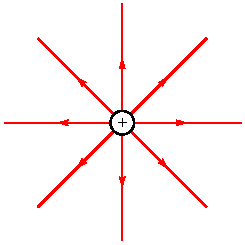
\includegraphics[height=96pt]{pos-charge}
	\end{minipage}
	\begin{minipage}{0.45\linewidth}
		\centering
		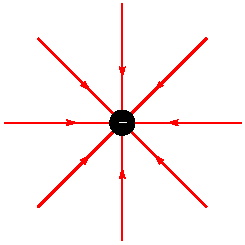
\includegraphics[height=96pt]{neg-charge}
	\end{minipage}
	
	\begin{center}
		radial fields around (a) an isolated positive charge, (b) an isolated negative charge
	\end{center}
\end{figure*}

\begin{figure*}[htp]
	\vspace*{-18pt}
	\begin{minipage}{0.3\linewidth}
		\centering
		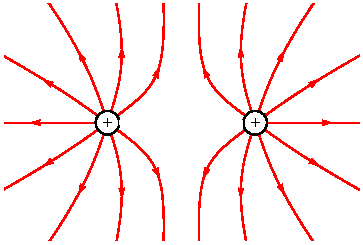
\includegraphics[height=96pt]{like-charges}
	\end{minipage}\hfill
	\begin{minipage}{0.3\linewidth}
		\centering
		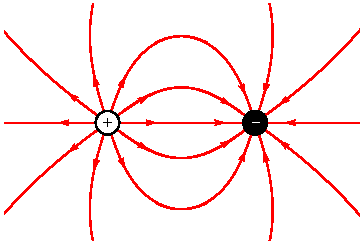
\includegraphics[height=96pt]{opposite-charges}
	\end{minipage}\hfill
	\begin{minipage}{0.3\linewidth}
		\centering
		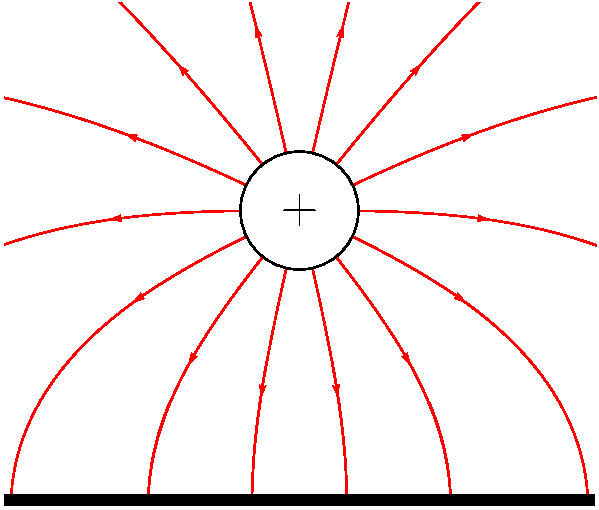
\includegraphics[height=96pt]{sheet-charge}
	\end{minipage}
	
	\begin{center}
		field between (c) two equal and like charges, (d) two equal but opposite charges,
		
		(e) a positive charge and a large conducting sheet that is earthed
	\end{center}
	
	
\end{figure*}

\subsection{Uniform electric fields}

\begin{marginfigure}
	\vspace{-12pt}
	\begin{center}
		\begin{circuitikz}[european resistors,xscale=0.95]
		\draw[thick] (-1.8,-1) -- (1.8,-1) (-1.8,1) -- (1.8,1);
		\draw[thick] (0,-1) -- (0,-2) node[midway,left]{\Large$-$} -- (3.2,-2)  (3.2,2) -- (0,2) -- (0,1)  node[midway,left]{\Large$+$};
		\draw[thick] (3.2,2) to[battery,l^=$V$] (3.2,-2);
		\foreach \x in {-1.5,-0.5,0.5,1.5} \draw[red,->] (\x,1) -- (\x,-1);
		\draw[<->] (2,-1) -- (2,1) node[midway,right]{$d$};
		\node[purple] at (0,0) {$E$};
		\end{circuitikz}
	\end{center}
	\vspace{-20pt}
\end{marginfigure}

Let's take two parallel metal plates and connect them to a high-voltage supply as shown, a charge in the region between the plates experiences a constant force regardless of its location in the field. The field strength is constant throughout the region, this field is said to be a \keypoint{uniform electric field}\index{electric field!uniform electric field}. Field lines of a uniform field are a set of parallel lines of equal spacing as shown on the right. If the two plates are separated by a distance of $d$, and a p.d. of $V$ is applied across them then magnitude of field strength of the uniform field is given by: $\tcbhighmath{ E = \frac{V}{d}}$

\noindent\textbf{proof:} The work done to bring a test charge $q$ from positive plate to negative plate: $ W=Fd=Eqd $, the change in electric potential energy is: $ \Delta E_p = q V$ (check \S\ref{ch:potential-difference} for meaning of p.d.). Work-energy theorem tells us these two must be equal: $ Eqd = qV$, so we find: $ {E=\frac{V}{d}} $

The electric field between metal plates points from high potential towards low potential.

\begin{figure}[ht]
	\centering
	\begin{minipage}{0.45\textwidth}
		\centering
		\begin{tikzpicture}
		\draw[thick] (-1.8,-1) -- (1.8,-1) (-1.8,1) -- (1.8,1);
		\draw[thick,white] (0,-1) -- (0,-1.1) node[ground]{};
		\draw[thick] (0,-1) -- (0,-1.5) node[below]{$-50$ V} (0,1.5) node[above]{$+30$ V} -- (0,1)  ;
		\foreach \x in {-1.5,-0.5,0.5,1.5} \draw[red,->] (\x,1) -- (\x,-1);
		\draw[<->] (2.25,-1) -- (2.25,1) node[midway,right]{10 cm};
		\node[purple] at (0,0) {$E$};
		\end{tikzpicture}
		\begin{equation*}
			E = \frac{V}{d} = \frac{(+30)-(-50)}{0.10} = 800\NpC
		\end{equation*}
	\end{minipage}\hfil
	\begin{minipage}{0.45\textwidth}
		\centering
		\begin{tikzpicture}
		\draw[thick] (-1.8,-1) -- (1.8,-1) (-1.8,1) -- (1.8,1);
		\draw[thick,white] (0,-1) -- (0,-1.5) node[below]{$-50$ V} (0,1.5) node[above]{$+30$ V} -- (0,1)  ;
		\draw[thick] (0,-1) -- (0,-1.1) node[ground]{} (0,1.5) node[above]{$-60$ V} -- (0,1) ;
		\node[right] at (0.3,-1.55) {earthed ($V_0=0$)};
		\foreach \x in {-1.5,-0.5,0.5,1.5} \draw[red,<-] (\x,1) -- (\x,-1);
		\draw[<->] (2.25,-1) -- (2.25,1) node[midway,right]{12 cm};
		\node[purple] at (0,0) {$E$};
		\end{tikzpicture}
		\begin{equation*}
		E = \frac{V}{d} = \frac{0-(-60)}{0.12} = 500\NpC
		\end{equation*}
	\end{minipage}
\end{figure}

\subsection{Equilibrium between electric force and weight}

\begin{marginfigure}
	\vspace{-16pt}
	\begin{center}
		\begin{tikzpicture}[xscale=1.1,yscale=1.35]
		\draw[thick] (-2,-1) -- (2,-1) (-2,1) -- (2,1);
		\draw[thick] (0,-1.6) -- (0,-1) node[midway,right]{\Large$+$} (0,1) -- (0,1.6) node[midway,right]{\Large$-$};
		\foreach \x in {-1.8,-0.6,0.6,1.8} \draw[red,->] (\x,-1) -- (\x,1);
		\draw[blue,thick,->] (0,0) -- (0,-0.75) node[right]{$W$};
		\draw[blue,thick,->] (0,0) -- (0,0.75) node[right]{$F_E$};
		\shade [ball color = green] (0,0) circle (0.08) node[left]{$+q$};
		\node[red] at (2.1,0.6) {$E$};
		\end{tikzpicture}
	\end{center}
	\vspace{-20pt}
\end{marginfigure}

A charged particle (e.g., a dust particle or an oil droplet) can be held stationary in a uniform electric field when the electric force is in equilibrium with weight of particle:

{
	\centering
	
	$ F_E = W \RA Eq = mg $
	
}
where field strength $E$ is given by: $E = \frac{V}{d}$

note that equilibrium is possible only if $F_E$ acts in opposite direction to $W$, so direction of the applied field depends on polarity of the charged particle

\newpage

\subsection{Deflection of a charged particle in a uniform field}

\begin{marginfigure}
	\vspace{-21pt}
	\begin{center}
		\begin{tikzpicture}[scale=1]
		\draw[very thick] (-2,-1) -- (2,-1) (-2,1) -- (2,1);
		\foreach \x in {-1.8,-0.6,0.6,1.8} \draw[red,->] (\x,-1) -- (\x,1);
		\draw[thick,blue,->] (0,-0.35) -- (0,0.7) node[below right]{$F$};
		\shade [ball color = green,dashed] (0,-0.35) circle (0.08);
		\draw [thick,blue!50,domain=-2:2,samples=20,smooth,variable=\x] plot (\x,{0.12*(\x-1)*(\x-1)-0.5});
		\node[red] at (2.1,0.6) {$E$};
		\draw[<->] (-3,0.4) node[left]{$y$} -- (-3,-0.4) -- (-2.2,-0.4) node[below]{$x$};
		\end{tikzpicture}
	\end{center}
	\vspace{-15pt}
\end{marginfigure}

A charged particle travelling in a uniform electric field would in general undergo a \emph{projectile-like} motion. This scenario is a frequent exam question context. We set up the coordinates such that electric field is along the $y$-axis, and $x$-axis is in the normal direction. We denote $x_0$, $y_0$ and $u_x$, $u_y$ as initial displacements and initial velocities at $t=0$.

The electric force only acts in $y$-direction, no force acts in $x$-direction.

\begin{compactenum}
	\item[--] in $x$-direction, particle maintains a constant velocity: $v_x = u_x$, $\,\, x = x_0 + u_x t$
	
	\item[--] in $y$-direction, particle accelerates uniformly: $v_y = u_y + a t$, $\,\, y=y_0 + u_y t + \frac{1}{2}at^2$
	
	where acceleration in $y$-direction is given by $ a=\frac{F}{m} = \frac{Eq}{m} \,\,$ (assuming weight is negligible)
\end{compactenum}

So the motion of a charged particle in a uniform electric field is analogous with projectile motion in a uniform gravitational field (see \S\ref{ch:projectile}), i.e., trajectory of charged particle is \emph{parabolic}.

\begin{marginfigure}
	\vspace{-15pt}
	\begin{center}
		\begin{tikzpicture}[scale=.96]
		\draw[very thick] (-2,-1) -- (2,-1) (-2,1) -- (2,1);
		\draw[<->] (-2,-1.8) -- (2,-1.8) node[midway,above] {$L=0.15 \text{ m}$};
		\draw[<->] (2.8,-1) -- (2.8,1) node[midway,right] {$d=0.10 \text{ m}$};
		\foreach \x in {-1.8,-0.6,0.6,1.8} \draw[red,<-] (\x,-1) -- (\x,1);
		\shade [ball color = green] (-3,0) circle (0.08) node[below]{$+q$};
		\draw[thick,blue,->] (0,-0.24) -- (0,-0.9) node[above right]{$F$};
		\shade [ball color = green,dashed] (0,-0.24) circle (0.08);
		\draw[->,thick,purple] (-3.5,0.3) -- (-2.5,0.3) node[midway,above]{$u$};
		\draw [thick,blue!50,domain=-2:2,samples=20,smooth,variable=\x] plot (\x,{-0.04*(\x+2.5)*(\x+2.5)+0.01}) (-2.0,0) -- (-3,0) (2.0,-0.8) -- ++(1,-0.36);
		\node[red] at (-2.1,-0.6) {$E$};
		\end{tikzpicture}
	\end{center}
	\vspace{-18pt}
\end{marginfigure}

\subsection{\piste Polar molecules in uniform electric fields}

Though the centre of positive and negative charges for a molecule do not necessarily overlap. This molecule is still electrically neutral, i.e., it has a zero net charge. Such a molecule is called a \emph{polar molecule}, and it could be affected by an electric field.

\begin{marginfigure}
	\vspace{-24pt}
	\begin{center}
		\begin{tikzpicture}[scale=1.8]
		\draw[thick] (-1.25,-1) -- (1.25,-1) (-1.25,1) -- (1.35,1);
		\draw[thick] (0,-1.5) -- (0,-1) node[midway,right]{\Large$-$} (0,1) -- (0,1.5) node[midway,right]{\Large$+$};
		\foreach \x in {-.9,.9} \draw[red,->] (\x,-1) -- (\x,1);
		\node[red] at (1.1,0.6) {$E$};
		\draw[brown,thick,rotate=35] (0,0) ellipse (0.6 and 0.3);
		\node[brown] at (38:0.35) {$-$};
		\node[brown] at (218:0.35) {$+$};
		\draw[thick, blue,->] (38:0.35) ++ (0,0.1) --++ (0,0.5) node[below right]{$F$};
		\draw[thick, blue,->] (218:0.35) ++ (0,-0.1) --++ (0,-0.5) node[above left]{$F$};
		\draw [dashed] (38:0.35) ++ (0,-0.1) --++ (0,-0.9);
		\draw [Green, <->] (38:0.35) ++ (-0.024,-0.9) --++ (-0.5,0) node[midway, above]{$L_\perp$};
		\end{tikzpicture}
	\end{center}
	\vspace{-20pt}
\end{marginfigure}

The diagram shows a polar molecule in a uniform field. The force on centre of positive charge and force on centre of negative charge are labelled as shown. This is a pair of equal but opposite forces that give rise to a resultant \emph{torque/moment}. Recall that the \emph{torque of couple} is defined as one force times perpendicular distance between the force pair (see \S\ref{ch:torque-of-couple}).

{
	\centering
	
	$\tau = F_E L_\perp \RA \tau Eq L_\perp$
	
}

This torque would cause the polar molecule to \emph{rotate}

\cleardoublepage

% ===== Chapter: particle-physics =====
\chapter{Sub-atomic Particles}

\section{Atomic structure}

\subsection{Atomic model}\label{ch:atomic-model}

All matter is composed of tiny particles called \keypoint{atoms}, each different element has its own type of atom \& the diagram below illustrates a simple atomic model\index{atomic model}.
\begin{figure*}[h]
	\vspace*{5pt}
	\centering
	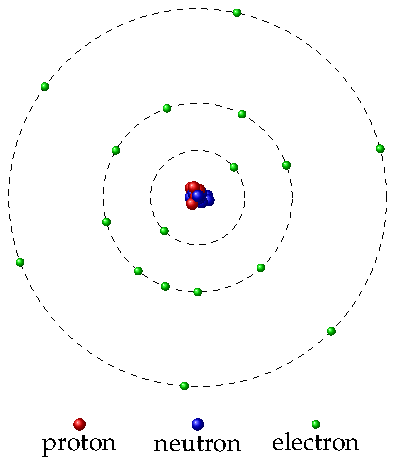
\includegraphics[height=180pt]{atomic-model.pdf}
	\vspace*{-20pt}
\end{figure*}

At the centre of each atom is the \keypoint{nucleus}\index{nucleus}. The radius of an atom $\sim 10^{-10} \sim 10^{-9} \text{ m}$ whereas the radius of a nucleus $\sim 10^{-15} \sim 10^{-14} \text{ m}$. Particles that make up the nucleus are called \keypoint{nucleons}\index{nucleon} and they come in two types, \keypoint{protons} and \keypoint{neutrons}\index{proton}\index{neutron}. Outside the nucleus are the \keypoint{electrons}\index{electron}, which move around the nucleus in a \emph{cloud}.

Protons, neutrons and electrons are the building blocks of all atoms and hence the building blocks for all matter

\cmt The properties of protons, neutrons and electrons are listed below:

\begin{compactenum}
	\item[--] charge of each proton and electron is the elementary charge unit: $e = 1.60 \times10^{-19} \text{ C}$
	
	\item[--] neutron has zero charge
	
	\item[--] a proton has very similar mass as a neutron
	
	\item[--] electron has much smaller mass than a nucleon (proton or neutron)
\end{compactenum}
\begin{figure*}
\begin{center}
	\begin{tabular}{|C{3.5cm}|C{1.6cm}|C{3.5cm}|C{2.8cm}|}
		\hline subatomic particle & charge & mass & location found \\ 
		\hline proton & $+e$ & $m_p = 1.67 \times 10^{-27}$ kg & nucleus \\ 
		\hline neutron & 0 & $m_n = 1.67 \times 10^{-27}$ kg & nucleus \\ 
		\hline electron & $-e$ & $m_e = 9.11 \times 10^{-31}$ kg & in outer atom \\ 
		\hline 
	\end{tabular}
\end{center}
\end{figure*}

\subsection{The $\alpha$-particle scattering experiment}

Hans Geiger, working in Rutherford's lab, did a series experiments in 1908 showing that alpha particles are "scattered" as they pass through thin layers of mica, and foils of gold and aluminium. In following year, joined by undergraduate Ernest Marsden, they did a series of experiments to untangle confusing results they observed. At the time of the experiment, the atom was thought to be analogous to a plum pudding (as proposed by J. J. Thomson), with the negatively-charged electrons (the plums) studded throughout a positive spherical matrix (the pudding). The scattering in this model was proposed to occur by many repeated collisions with the electrons and the alpha particles should only be deflected by small angles as they pass through.

The plum-pudding model predicts that deflection of $\alpha$-particles should be uniformly distributed around the central beam, but there is no reason that an $\alpha$-particle would undergo a large change in its direction of motion, like a cannonball hitting a piece of paper and rebounding backwards. The results of the scattering experiment meant that the plum-pudding model had to be overturned. In order to explain the experimental observations, Rutherford then put forward the new model which now bears his name.
\definecolor{mylightblue}{RGB}{220,228,255}
\definecolor{myblue}{RGB}{183,191,229}
\definecolor{mydarkblue}{RGB}{50,70,190}
\begin{marginfigure}
    \begin{tikzpicture}[scale=1]
  \coordinate (O)  at (0,0);
  \draw[mylightblue,fill] (O) circle (50pt);
  \draw[mydarkblue,thick] (O) circle (50pt) node[above right=34pt] {$+Ze$};
  \fill[radius=0.8pt,mydarkred]
    ( 0.20, 1.20)  circle node[above right=-1pt,scale=0.75] {$-e$}
    ( 0.10, 0.30)  circle node[above right=-1pt,scale=0.75] {$-e$}
    ( 0.68, 0.67)  circle node[above right=-1pt,scale=0.75] {$-e$}
    ( 1.05,-1.10)  circle node[above left =-1pt,scale=0.75] {$-e$}
    ( 0.75,-0.12)  circle node[      right= 2pt,scale=0.75] {$-e$}
    ( 0.21,-1.30)  circle node[above left =-1pt,scale=0.75] {$-e$}
    ( 0.18,-0.55)  circle node[above left =-1pt,scale=0.75] {$-e$}
    (-0.80, 0.60)  circle node[above left =-1pt,scale=0.75] {$-e$}
    (-0.50, 1.21)  circle node[above right=-1pt,scale=0.75] {$-e$}
    (-0.40, 0.05)  circle node[above left =-1pt,scale=0.75] {$-e$}
    (-0.58,-0.95)  circle node[above left =-1pt,scale=0.75] {$-e$}
    (-1.10,-0.20)  circle node[above left =-1pt,scale=0.75] {$-e$};
\end{tikzpicture}
\caption{The Plum pudding model of the atom.}
\end{marginfigure}

One of the most important experiments they carried out was the \keypoint{$\alpha$-particle scattering experiment}\index{$\alpha$-particle scattering experiment} in which \emph{Hans Geiger} and \emph{Ernest Marsden} studied atomic structure by firing $\alpha$-particle beam towards a thin gold foil at the University of Manchester.

\begin{figure}[!ht]
	\centering
	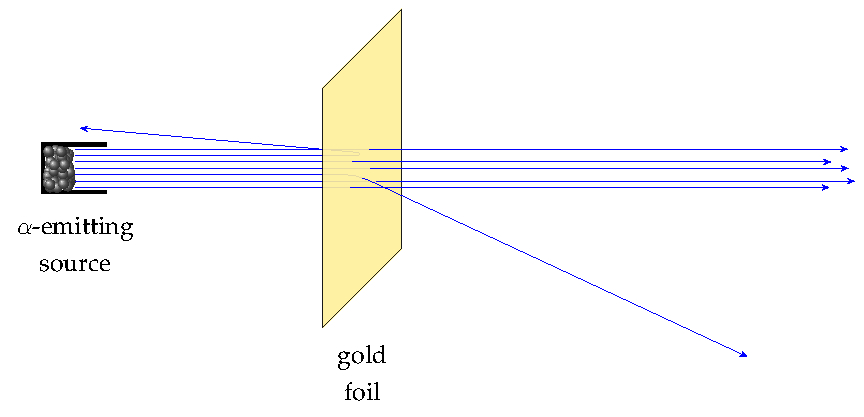
\includegraphics[height=180pt]{alpha-scattering}
	\caption{Rutherford's $\alpha$-particle scattering experiment}
\end{figure}

\begin{figure}[!ht]
	\centering
	\begin{tikzpicture}[scale=1.33]
		\shade[ball color=Gold] (0,0) circle (.2);
		\node[right, twoline] at (0.3,0) {gold\\nucleus}; 
		\draw[blue,->] (-4,0.03) -- (-0.4, 0.03) arc(-90:86:0.04) --++ (176:2.5);
		\draw[blue,->] (-4,1) -- (3, 1);
		\draw[blue,->] (-4,-1.2) -- (3, -1.2);
		\draw[blue,->] (-4,-0.5) -- (-1,-0.5) arc(90:65:4) --++ (-25:2.4);
	\end{tikzpicture}
	
	\caption{paths of $\alpha$-particles as they approach and pass by a gold nucleus}
\end{figure}

The main experimental results of the experiments are:

\begin{compactitem}
	\item[--] most $\alpha$-particles pass straight through the foil with almost no deflection
	
	\item[--] very few $\alpha$-particles (about 1 in $10^4$) are deflected by large angles.
\end{compactitem}

To explain the observations, Rutherford concluded the following about nature of atoms

\begin{compactitem}
	\item[--] most space in an atom is empty
	
	(so most $\alpha$-particles merely pass through empty space without deflection)
	
	\item[--] there is a tiny positively-charged core, called the nucleus, at centre of an atom
	
	(so only a small fraction of $\alpha$-particles would interact with the nucleus)
	
	\item[--] almost all mass of the atom is concentrated in the nucleus
	
	(so interaction is influential if nucleus happens to sit on the path of $\alpha$-particle beam)
\end{compactitem}

Based on these understandings, Rutherford proposed the atomic model introduced in \S\ref{ch:atomic-model}. This model is now known as \emph{Rutherford's model}, or \emph{planetary model of the atom}\footnote{\piste 
	 Rutherford originally suggested that electrons rotate around the nucleus in \emph{circular} orbits due to attractive electrostatic force, like the planets orbit around the sun. This is why Rutherford's model of atomic structure is also called \emph{the planetary model of the atom}.
	 
	 However, later studies showed that Rutherford's model had its own problems. Classical electromagnetic theory suggests that any charged particle in accelerated motion would radiate energy, so the orbiting electrons will gradually lose all its energy and fall into the nucleus. An atom can never be stable if the Rutherford's model is correct. The full description of the atomic structure requires the understanding of the \emph{quantum} behaviour of electrons, which are described by \emph{probability waves}. Electrons actually do not move in circular orbits but have a certain probability to be anywhere in space at any time, forming an \emph{electron cloud}.
 }

\subsection{Nuclide notation}

\keypoint{Nuclides} are specific types of atoms or nuclei. A nuclide is uniquely defined by its \keypoint{proton number} $Z$ and its \keypoint{nucleon number} $A$. A nuclide is usually denoted as $\tcbhighmath{_Z^A X}$, where $X$ is the chemical symbol for the element. 

\cmt By definition, $Z$ gives number of protons, $A$ gives number of nucleons, as a consequence, number of neutrons is given by $N = A-Z$. Proton number $Z$ can be further interpreted as \keypoint{charge number} of the particle \index{charge number}. Recall that each proton carries charge $+e$, and neutrons are chargeless so $Z$ further determines electrical charge of the nucleus: \begin{empheq}[box=\tcbhighmath]{equation*}{Q = +Ze}\end{empheq}.

This extension will be important when we deal with other particles later in this chapter.

The nucleon number $A$ can be interpreted as \keypoint{mass number} of the particle \index{mass number}, each proton and neutron is of approximately the same mass so the mass of nucleus is determined by total number of protons and neutrons: \begin{empheq}[box=\tcbhighmath]{equation*}{m = A\text{u}}\end{empheq}.

where $1 \text{ u} = 1.66\times10^{-27} \text{ kg}$ is the \keypoint{unified atomic mass unit}
\footnote[][-4cm]{Note that the unified atomic mass ($1.661\times10^{-27} \text{ kg}$), formally defined as one twelfth of the mass of an carbon-12 atom, is slightly less than the mass of a \emph{free} proton ($m_p=1.673\times10^{-27} \text{ kg}$ or that of a \emph{free} neutron ($m_n=1.675\times10^{-27} \text{ kg}$). This is because energy goes out when protons and neutrons combine to form a nucleus, and this would be associated with a decrease in the mass as suggested by \emph{Albert Einstein's mass-energy equivalence principle}. You can think of $\text{u}$ as the average mass of a proton or a neutron when a group of them squeeze together. If you want to find out the mass of a nucleus, you should use $\text{u}$. But if you are dealing with a single proton or a single neutron, you should use $m_p$ and $m_n$ instead.}

Using this notation, protons, neutrons and electrons can be represented by: \begin{empheq}[box=\tcbhighmath]{equation*}{^1_1\text{p}} \hspace{1cm}{^1_0\text{n}}\hspace{1cm}{^{\phantom{-}0}_{-1}\text{e}}\end{empheq}

\subsection{Chemical properties of elements}

The chemical properties of an atom depend on the number of electrons, the proton number $Z$ gives us more than just the \keypoint{atomic number} of the element. In a neutral atom, there are same number of protons as electrons so atoms of same chemical properties, i.e., atoms of same element have same proton number. That said, atoms of same chemical properties can have different nuclei. \keypoint{Isotopes} of an element have same number of protons but a different number of neutrons\index{isotope}.

\subsection{Radioactivity}

\subsection{Radioactive decays}

If a nucleus is unstable then it may break down by releasing radiation from the nucleus, this process is called \keypoint{radioactive decay}\index{radioactive decay}. The three most common types of radioactive decays are $\alpha$-decay, $\beta$-decay and $\gamma$-decay. 

Radioactive decays are \emph{spontaneous} and decay events are independent of outside conditions, such as temperature, pressure, etc. Whether one nucleus is about to decay is also independent of the other nuclei around it. 

Radioactive decays depend only on the internal stability of the nucleus, they are truly \emph{random}. 

\subsection{Properties of $\alpha$-, $\beta$- \& $\gamma$-radiation}

\subsection*{Nature of \texorpdfstring{$\alpha$}{\textalpha}-radiation}

$\alpha$-particles are \emph{helium nuclei}, each made up of two protons and two neutrons\index{radioactive decay!$\alpha$-decay}

an $\alpha$-particle therefore carries a positive charge of 2$e$, and a mass of 4u

$\alpha$-particles emitted from a given source travel at almost the same speed

speed of $\alpha$-particles is usually less than one-tenth of the speed of light

\subsection*{Nature of \texorpdfstring{$\beta$}{\textbeta}-radiation}

$\beta$-radiation is a beam of high-speed \emph{electrons}\index{radioactive decay!$\beta$-decay}

$\beta$-particle is negatively charged and very light compared with a nucleus

$\beta$-particles travel at very high speeds close to the speed of light

\subsection*{Nature of \texorpdfstring{$\gamma$}{\textgamma}-radiation}

$\gamma$-radiation, or $\gamma$-photon, is a high-frequency electromagnetic wave\index{radioactive decay!$\gamma$-decay}

$\gamma$-radiation is electrically neutral and has no mass

like any other electromagnetic wave, $\gamma$-radiation travels at the speed of light in vacuum

\subsection*{Brief summary for nature of \texorpdfstring{$\alpha$}{\textalpha}-, \texorpdfstring{$\beta$}{\textbeta}- \& \texorpdfstring{$\gamma$}{\textgamma}-radiation}

\begin{center}
	{\renewcommand{\arraystretch}{1.2}
	\begin{tabular}{|C{2cm}|C{2.8cm}|C{2.8cm}|C{4.2cm}|}
	\hline  & $\alpha$-radiation & $\beta$-radiation & $\gamma$-radiation \\ 
	\hline nature & helium nucleus & electron & electromagnetic wave \\ 
	\hline notation & $^4_2\alpha$ & $^{\phantom{-}0}_{-1}\beta$ & $^0_0\gamma$ \\
	\hline mass & 4u & $\frac{1}{1800}\text{u} \approx 0$ & 0 \\[4pt]
	\hline charge & $+2e$ & $-e$ & 0 \\ 
	\hline speed & $0.1c$ & $0.99c$ & $c$ \\
	\hline
    \end{tabular}
    }
\end{center}

%\begin{question}
%	Some radioactive sources are found to contain helium gas. How do you explain that?
%\end{question}

%\begin{question}
%	$\alpha$-particles are used in the scattering experiment to investigate the structure of an atom. Is it appropriate to use a $\beta$-emitting source to do the same experiment? Explain your reasons.
%\end{question}

\begin{figure}[ht]
	\centering
	\begin{tikzpicture}
	\draw[thick] (-3,-1) -- (3,-1) (-3,1) -- (3,1);
	\draw[thick] (0,-1) -- (0,-2) node[midway, right] {$-$};
	\draw[thick] (0,1) -- (0,2) node[midway, right] {$+$};
	\draw[thick, purple, ->] (-4,0) -- (4, 0) node[right] {$\gamma$};
	\draw[thick, Green, ->] (-4,0.05) -- (-3,0.05) parabola (-2.4,1) node[below right]{$\beta$};
	\draw[thick, blue, ->] (-4,-0.05) -- (-3,-0.05) parabola (3,-0.85) --++ (-14.93:1) node[right] {$\alpha$};
	\end{tikzpicture}
\end{figure}

\subsection*{Penetration \& ionising power}

Different radiation have different abilities to pass through materials, $\alpha$-, $\beta$- and $\gamma$- radiation are able to knock out orbital electrons from an atom so radiation can cause the originally neutral atom to become charged. This process is called \keypoint{ionising}\index{ionising power}. 

Greater ionising ability would imply lower penetration power. 

$\gamma$-radiation is very penetrative but has very weak ionising power, $\gamma$-radiation is not charged, and hence it does not interact strongly with electrons. A $\gamma$-photon loses all its energy in single collision and gets absorbed i.e., one $\gamma$-photon can only ionise one atom so it has few collisions with electrons, so $\gamma$-radiation is not very ionising

$\alpha$- and $\beta$-radiation more ionising than $\gamma$-radiation because $\alpha$- and $\beta$-radiation are charged, making them interact with electrons more easily.

$\alpha$-particles are the most highly ionising, recall $\alpha$-particles are much more massive than electrons so one $\alpha$-particle can knock out many electrons before it loses all of its kinetic energy. Also $\alpha$-particles travel at low speeds, so frequent collision events take place in short range. $\alpha$-radiation therefore has strong ionising ability but weak penetration power.

The table below summarises penetration and ionising power of radioactive radiation:
\begin{figure*}

\begin{center}
	\begin{tabular}{|C{3cm}|C{3.2cm}|C{3.2cm}|C{3.2cm}|}
		\hline  & $\alpha$-radiation & $\beta$-radiation & $\gamma$-radiation \\ 
		\hline \multirow{2}{3.2cm}[-20pt]{penetration power} & low & fair & high \\
		 & stopped by thick cardboard or a few centimetres of air & stopped by metal plates of a few millimetres thick & stopped by thick lead or concrete of a few centimetres\\
		\hline ionising power & high & fair & low \\ 
		\hline
	\end{tabular} 
\end{center}
\end{figure*}

\subsection{Laws of conservation}

Some of the conserved quantities during any decay process are:
\begin{itemize}
    \item conservation of \emph{electric charge}
    \item conservation of \emph{charge number} ($Z$)\index{charge number}
    \item conservation of \emph{mass-energy}\index{mass-energy conservation}
    \item conservation of \emph{mass number} ($A$)\index{mass number}
    \item conservation of \emph{momentum} (review \S\ref{ch:momentum-conservation} if needed)
\end{itemize}

\subsection{Decay equations}

Using nuclide notation, radioactive decay processes can be described by \emph{decay equations} - the conserved quantities provide a simple guideline to write the decay equations 

\begin{compactenum}
	\item[--] sum of charge numbers ($Z$) on both sides of the equation should add up
	
	\item[--] sum of mass numbers ($A$) on both sides of the equation should add up
\end{compactenum}

The first reported nuclear reaction was credited to Ernest Rutherford. By firing $\alpha$-particles into pure nitrogen, Rutherford observed the ejection of hydrogen nuclei from the gas, which is now regarded as the discovery of protons. This reaction can be given by:
\begin{equation*}
_{\phantom{0}7}^{14} \text{N} + _2^4 \alpha \longrightarrow _{\phantom{0}8}^{17} \text{O} + _{1}^{1} \text{p} 
\end{equation*} 

One reaction that is widely used to power nuclear reactors is the induced fission of uranium-235. The reaction can be triggered by bombarding the uranium-235 nuclei with slow neutrons. The uranium nucleus would split up into two lighter nuclei and release a large amount of energy. One of such reactions can be described by:
\begin{equation*}
 _{\phantom{0}92}^{235} \text{U} + _0^1 \text{n} \longrightarrow _{\phantom{0}56}^{141} \text{Ba} + _{36}^{92} \text{Kr} + 3_0^1 \text{n} 
\end{equation*} 

\subsection*{Equation for \texorpdfstring{$\alpha$}{\textalpha}-decays}\index{radioactive decay!$\alpha$-decay}

If a nuclide $_Z^A X$ undergoes $\alpha$-decays, then we have:
\begin{empheq}[box=\tcbhighmath]{equation*}{_Z^A X \longrightarrow _{Z-2}^{A-4} Y + _2^4\alpha}
\end{empheq}

The original nucleus lost two protons and two neutrons during the decay, on both sides of the equation, there are $Z$ protons and $(A-Z)$ neutrons therefore $\alpha$-decay simply is an $\alpha$-particle escaping from the nucleus.

\begin{equation*}
	_{\phantom{0}92}^{238} \text{U} \longrightarrow _{\phantom{0}90}^{234} \text{Th} + _2^4\alpha 
\end{equation*}

\subsection*{Equation for \texorpdfstring{$\gamma$}{\textgamma}-decays}\index{radioactive decay!$\gamma$-decay}

$\gamma$-radiation has zero charge and zero mass, so decay equation is very straightforward:
\begin{empheq}[box=\tcbhighmath]{equation*}{_Z^A X \longrightarrow _{Z}^{A} X + _0^0\gamma}
\end{empheq}

since $\gamma$-radiation is pure energy, so there is no change of structure of the nucleus in any way

\subsection{Fundamental particles}

In early 20th century, lots of new subatomic particles were discovered in \emph{cosmic rays} and \emph{particle accelerators}. Many of these particles did not fit into the model where proton, neutrons and electrons are the fundamental building blocks for the physical world. To incorporate these subatomic particles discovered at the time, physicist worked out the \keypoint{Standard Model of particle physics}.\footnote[][-3cm]{The theory of the Standard Model was developed in stages since the 1950s, through the work of many great scientists, with the current formulation being finalized in the 1970s.\index{Standard Model}
	\begin{compactitem}
		\item[--] \emph{Chen Ning Yang} and \emph{Robert Mills} developed the concept of \emph{gauge theory}, to provide an explanation for the interaction between elementary particles.
		
		\item[--] \emph{Sheldon Glashow} proposed the symmetry group that forms the basis of the accepted \emph{electroweak theory}, in which the electromagnetic interaction and weak interactions are unified into a single force.
		
		\item[--] \emph{Peter Higgs} and two other groups proposed the \emph{Higgs mechanism} that give rise to mass generation for elementary particles without violating gauge theory through a process called \emph{symmetry breaking}.
		
		\item[--] \emph{Steven Weinberg} and \emph{Abdus Salam} incorporated the Higgs mechanism into Glashow's theory, finalizing the unified electroweak theory.
		
		\item[--] \emph{David Gross}, \emph{Frank Wilczek}, \emph{David Politze}, and many others developed \emph{quantum chromodynamics}, the theory of the strong interaction, into its modern form.
		
		\item[--] $\cdots$
	\end{compactitem}

Being the most accurate accurate scientific theory known to human beings, the Standard Model is now regarded as one of the greatest triumphs of modern physics. The theory not only describes the particles known to scientists, but also predicted new particles, including the \emph{Higgs boson}. }

\subsection{Particles \& anti-particles}

For any particle $\text{p}$, there exists an associated \keypoint{anti-particle} $\bar{\text{p}}$\index{anti-particle}

\cmt an anti-particle has the same mass but opposite charge to its counterpart

\cmt when a particle meets its anti-particle, they \keypoint{annihilate} each other and produce two $\gamma$-photons

combined mass-energy of the pair is converted into electromagnetic energy
\footnote{The energy release from the annihilation of  particle pairs could be potentially used a energy source. The idea of using antimatter to power spaceships or weapons can be found in many science fiction stories.}

\subsection{Quarks \& hadrons}

One type of the elementary matter particle is the \keypoint{quark}\index{quark}

\cmt quarks come in six varieties, or six \keypoint{flavours}

they are \keypoint{up} (u), \keypoint{down} (d), \keypoint{strange} (s), \keypoint{chartm} (c), \keypoint{top} (t), \keypoint{bottom} (b)

\cmt each quark carries an electric charge, as given in the table below

\begin{center}
	{\renewcommand{\arraystretch}{1.35}
		\begin{tabular}{|C{3cm}|C{2cm}|C{2cm}|}
			\hline  & u & d \\
			 quarks & c & s \\
			  & t & b \\
			\hline charge & $+\frac{2}{3}e$ & $-\frac{1}{3}e$ \\[3pt]
			\hline
		\end{tabular}
	}
\end{center}

note that all quarks carry a \emph{fraction} of the elementary charge unit\footnote{Each horizontal line in the table is known as a \emph{generations} of quarks. As you can see, there are three generations of quarks.}

Quarks can combine to form composite particles called \keypoint{hadrons} \index{hadron}, there are two ways that several quarks can make up a hadron:

\begin{compactenum}
	\item[--] hadrons can be made up of three quarks (qqq), called \keypoint{baryons} \index{baryon}
	
	members of the baryon family include protons and neutrons
	
	a proton consists of two up quarks and one down quark (uud) \index{proton}
	
	a neutron consists of one up quark and two down quarks (udd) \index{neutron}
	
	\item[--] hadrons can also be made up of one quark and one anti-quark (q$\bar{\text{q}}$), called \keypoint{mesons} \index{meson}
	
	you don't need to memorise any example of meson
	
	you are only required to identify if a particle is a meson given the quark composition
\end{compactenum}

\cmt quarks and hadrons are affected by the \keypoint{strong nuclear force}\index{strong nuclear force}

strong nuclear force is a very short-ranged attractive force

\begin{compactenum}
	\item[--] it is responsible for hold quarks close together to from hadrons

	\item[--] it is also responsible for the attraction between hadrons
	
	for example, protons and neutrons are held together in a nucleus by strong force
	\footnote{For a small nucleus, strength of strong nuclear force is way greater than the electric repulsion between positively-charged protons, hence the force bind protons and neutrons together forming a stable nucleus. However, since the strong nuclear force has a very short range, the repulsive electrostatic force between the protons might dominate the attractive nuclear force for an over-sized nucleus. Such large nuclei become unstable and are likely to undergo \emph{radioactive decays}.}
\end{compactenum}

\cmt quarks only exist in hadrons, i.e., there are no single free quarks in nature\footnote{This is known as the \emph{confinement}, a consequence that is closely related to the fact that interaction between quarks are weak at high energies or smaller length scales but strong at low energies or large length scales, a feature of strong nuclear forces known as \emph{asymptotic freedom}.}

\subsection{Leptons}

Another type of the elementary matter particle is the \keypoint{lepton}\index{lepton} - they are not affected by strong nuclear forces. Members of the lepton family include electrons (e), neutrinos ($\nu$), muons ($\mu$), taons ($\tau$)\footnote{Just like the quarks, leptons also come in three \emph{generations}. Each generation of leptons consists of an electron-like particle and its associated neutrino.}

in A-Level exams, you only need to know electrons (e) and neutrinos ($\nu$)

\cmt for each particle, one can assign a \keypoint{lepton number} $L$

\begin{compactitem}
	\item[--] a lepton has lepton number $L=+1$
	
	\item[--] an anti-lepton has lepton number $L=-1$
	
	 \item[--]any other particle has lepton number $L=0$
\end{compactitem}

classification of sub-atomic particles within the A-Level syllabus is summarised below\footnote[][-2cm]{This is an over-simplified version of the Standard Model. I only included the particles that you need to know for the A-Level exams. There are a lot of missing pieces that are way beyond the scope of our course, so please don't take this mindmap too seriously.}

\begin{figure*}[ht]
	\centering
	\begin{tikzpicture}
%\draw[help lines, gray!30, step=0.5] (0,-5) grid (15,5);
%\foreach \x in {1,2,...,15} \node[below] at (\x,0) {\x};
%\foreach \y in {-5,-4,...,5} \node[left] at (0,\y) {\y};
	% root / fundamental particles
	\draw (2.5,0.4) -- (3.5,0.4) (4.5, -.6) -- (3.5,-0.6) -- (3.5, 2.5) -- (4.5, 2.5);
	\draw[rounded corners, fill=white] (0.1,-0.3) rectangle (2.5,1.1);
	\draw (1.3,0.4) node[twolinecap] {fundamental\\particles};
	% quarks
	\draw[rounded corners, fill=white] (4.3,2.2) rectangle (5.9, 2.8);
	\draw (5.1, 2.5) node {quarks};	
	\draw (5.0, 2.1) -- (4.6, 1.6);
	\draw (5.2, 2.1) -- (5.6, 1.6);
	\node at (4.6, 1.4) {u};
	\node at (5.6, 1.4) {d};
	\node at (4.6, 0.9) {{\scriptsize $+\frac{2}{3}e$}};
	\node at (5.6, 0.9) {{\scriptsize $-\frac{1}{3}e$}};
	% leptons
	\draw[rounded corners, fill=white] (4.3,-.4) rectangle (5.9, -1.0);
	\draw (5.1, -.7) node {leptons};
	\draw (5.0, -1.1) -- (4.6, -1.6) node[below]{e};
	\draw (5.2, -1.1) -- (5.6, -1.6) node[below]{$\nu$};
	\node at (4.6, -2.2) {{\scriptsize $-e$}};
	\node at (5.6, -2.2) {{\scriptsize $0$}};
	% hadrons
	\draw[dashed, ->] (5.9, 2.5) -- (8.1,2.5) node[midway, above]{make up};
	\draw[rounded corners, fill=white] (8.1,2.2) rectangle (9.9, 2.8);
	\draw (9, 2.5) node {hadrons};
	% baryons
	\draw (9.9, 2.5) -- (10.5, 2.5) -- (10.5, 3.5) -- (12, 3.5) node[midway, above]{(qqq)};
	\draw[rounded corners, fill=white] (12,3.2) rectangle (13.8, 3.8);
	\draw (12.9, 3.5) node {baryons};
	\draw (12.8, 3.1) -- (12.4, 2.6) node[below]{p};
	\draw (13.0, 3.1) -- (13.4, 2.6) node[below]{n};
	% mesons
	\draw (10.5, 2.5) -- (10.5, 1.5) -- (12, 1.5) node[midway, above]{(q$\bar{\text{q}}$)};
	\draw[rounded corners, fill=white] (12,1.2) rectangle (13.8, 1.8);
	\draw (12.9, 1.5) node {mesons};
	\end{tikzpicture}
	\caption{a coarse guide for classifying sub-atomic particles in A-Level physics}
\end{figure*}

\subsection{\texorpdfstring{$\beta$}{\textbeta}-decays}\index{radioactive decay!$\beta$-decay}

there exists positron, anti-particle of electron, so there are two types of $\beta$-particles: $\beta^-$ and $\beta^+$

hence two types of $\beta$-decays are possible: $\beta^-$-decay and $\beta^+$-decay

\subsection*{\texorpdfstring{$\beta^-$}{\textbeta\textsubscript{-}}-decay revisited}

a neutron changes into a proton during a $\beta^-$-decay: $\boxed{_0^1 \text{n} \longrightarrow _1^1 \text{p} + _{-1}^{\phantom{+}0}\beta + _0^0 \bar{\nu}} $

we have learned about the quark structures of protons (uud) and neutrons (udd)

therefore $\beta^-$-decay process at a more fundamental level is: \begin{empheq}[box=\tcbhighmath]{equation*}{\text{d} \longrightarrow \text{u} + \beta^- + \bar{\nu}} \end{empheq}

\subsection*{\texorpdfstring{$\beta^+$}{\textbeta\textsubscript{+}}-decay}

$\beta^+$-decay occurs when a proton changes into a neutron and emits a positron

$\beta^+$-decay process is described by the equation: \begin{empheq}[box=\tcbhighmath]{equation*}{_1^1 \text{p} \longrightarrow _0^1 \text{n} + _{+1}^{\phantom{+}0}\beta + _0^0 \nu} \end{empheq}

in terms of quarks, $\beta^+$-decay can be rewritten as: \begin{empheq}[box=\tcbhighmath]{equation*}{\text{u} \longrightarrow \text{d} + \beta^+ + \nu} \end{empheq}

\cmt nature of $\beta$-decay processes is the transformation of quark flavours

the interaction responsible for this transformation is the \keypoint{weak nuclear force}\index{weak nuclear force}

\cmt there is yet another law of conservation -- the \keypoint{conservation of lepton number}

we can use lepton number to predict whether a neutrino or an anti-neutrino is emitted

	
\section{End-of-chapter questions}

\subsection*{Atomic structure}

 

\subsection*{Radioactive decays}
	

\subsection*{Nuclear equations}

\subsection*{Fundamental particles}

\cleardoublepage

% ===== Chapter: 18-circular-motion =====
\chapter{Circular Motion}

\section{Angular quantities}

Movement or rotation of an object along a circular path is called \keypoint{circular motion}, to describe a circular motion, we can use \emph{angular quantities}, which turn out to be more useful than linear displacement , linear velocity , etc.

\subsection{Angular displacement}

\begin{ilight}
	\keypoint{Angular displacement}\index{angular displacement} is angle swiped out by object moving along circular
\end{ilight}

\begin{marginfigure}
	\centering
	\vspace*{-8pt}
	\begin{tikzpicture}[scale=0.8]
		\draw[dotted,thick] (0,0) circle(2);
		\draw[->,thick,blue] (2,0) arc (0:70:2);
		\draw (2,0) -- (0,0) node[midway,below]{$r$} -- (70:2);
		\draw[->,thick] (0.4,0) arc (0:70:0.4);
		\node at (35:0.6) {$\theta$};
		\node at (35:2.2) {$s$};
	\end{tikzpicture}
\end{marginfigure}

unit: $[\theta]=\rad \quad$ (natural unit of measurement for angles)

conversion rule: $2\pi \rad = 360^\circ$

\cmt if two radii form an angle of $\theta$, then length of arc: $s=r\theta$

two radii subtending an arc of same length as radius form an angle of one \keypoint{radian}\index{radian}

\subsection{Angular velocity}

Angular velocity describes how fast an object moves along a circular path

\begin{ilight}
	\keypoint{Angular velocity}\index{angular velocity} is defined as angular displacement swiped out per unit time: $\tcbhighmath{\omega = \frac{\Delta \theta}{\Delta t}}$
\end{ilight}

\cmt unit of: $[\omega] = \radps$, also in radian measures

\cmt angular velocity is a \emph{vector} quantity that points in a direction normal to the plane of circular motion but in A-level course, we treat angular velocity as if it is a scalar. Angular velocity and angular speed may be considered to be the same idea

Angular and linear velocity are closely related: in interval $\Delta t$, distance moved along arc $$\Delta s=v\Delta t=r \Delta\theta \RA \omega = \frac{\Delta \theta}{\Delta t} = \frac{v}{r} \RA \tcbhighmath{v=\omega r}$$

this relation between linear speed and angular speed holds at any instant

\subsection{Uniform circular motion}

Consider the simplest possible circular motion $\longrightarrow$ circular motion with constant $\omega$

\begin{marginfigure}
	\centering
	\begin{tikzpicture}[scale=0.6]
	\draw (0,0) circle [radius=3];
	\foreach \s in {0,140,230}
	{
		\draw [purple, thick, ->] (\s:3) -- ++(\s+90:2.5) node[right]{$v$};
		\draw [thick, dashed] (\s:3) -- (0,0);
		\draw [thick] (\s:2.7) -- ++(\s+90:0.3) -- ++(\s:0.3);
	}
	\end{tikzpicture}
\end{marginfigure}

analogy with linear motion with constant $v$

uniform linear motion: $s=vt$

displacement $s \leftrightarrow \theta$, velocity $v \leftrightarrow \omega$

for uniform circular motion, one has: $$\tcbhighmath{\theta=\omega t}$$

\cmt time taken for one complete revolution is called \keypoint{period} $T$

in one $T$, angle swiped is $2\pi$, so $$\tcbhighmath{\omega=\frac{2\pi}{T}}$$

\cmt uniform circular motion is still \emph{accelerated} motion

speed is unchanged, but \emph{velocity} is changing

direction of velocity always \emph{tangential} to its path, so direction of velocity keeps changing

in general, any object moving along circular path is accelerating

\subsection{Centripetal acceleration}

\rcyskip

\begin{ilight}
	\keypoint{Centripetal acceleration} is the acceleration due to the change in direction of velocity vector, it points toward the centre of circular path
\end{ilight}

consider motion along a circular path from $A$ to $B$ with constant speed $v$

under small (infinitesimal) duration of time $\Delta t$\footnote{A more rigorous derivation can be given by using differentiation techniques}

\begin{figure}[ht]
	\centering
		\begin{tikzpicture}[scale=1]
		\draw [thick, dashed] (70:4) arc [radius=4, start angle=70, end angle=110];
		\draw [thick] (80:1.5) arc [radius=1.5, start angle=80, end angle=100];
		\foreach \s in {80,100}
		{
			\draw [purple, thick, ->] (\s:4) -- ++(\s-90:1.2) node[above]{$v$};
			\draw [thick, dashed] (\s:4) -- (0,0);
		}
		\draw (80:4) node[above]{$B$};
		\draw (100:4) node[above]{$A$};
		\draw (0,1.5) node[above]{$\Delta \theta$};
		\draw [thick,->] (2.5,2) --++ (2,0);
		\draw [purple, thick, ->] (5.5,2) -- ++(10:1) node[above] {$v$} -- ++(10:1);
		\draw [purple, thick, ->] (5.5,2) -- ++(-10:1) node[below] {$v$} -- ++(-10:1);
		\draw [purple, thick, ->] (7.470,2.347) -- ++ (0,-0.347) node[right]{$\Delta v$} -- ++ (0,-0.347);
		\draw (5.6,1.9) node[below]{$\Delta \theta$};
		\draw (5.5,2) ++ (-10:0.5) arc(-10:10:0.5);
		\end{tikzpicture}
\end{figure}

	change in velocity: $\Delta v = 2v\sin\frac{\Delta \theta}{2} \approx v \Delta \theta \quad$ (as $\Delta \theta \to 0$, $\sin \Delta \theta \approx \Delta \theta$)
	
	acceleration: $a = \frac{\Delta v}{\Delta t} \approx v \frac{\Delta \theta}{\Delta t} = v \omega \quad$ (as $\omega = \frac{\Delta \theta}{\Delta t}$)
	
	recall relation $v = \omega r$, we find centripetal acceleration: $$\tcbhighmath{a_c = \frac{v^2}{r} = \omega^2 r}$$\index{centripetal acceleration}

\cmt direction of centripetal acceleration: always towards centre of circular path
	
\cmt centripetal acceleration is only responsible for the change in \emph{direction} of velocity

change in \emph{magnitude} of velocity will give rise to \emph{tangential acceleration}

this is related to \emph{angular acceleration}\footnote{Angular acceleration is analogous to linear acceleration $\alpha$, defined as rate of change of angular velocity: $\alpha = \frac{\dd \omega}{\dd t} = \frac{\dd^2 \theta}{\dd t^2}$ \piste. Similar to $v=\omega r = \ddt{s}$, the relation $a=\alpha r = \ddt{v}$ also holds.}  , which is beyond the syllabus

\subsection{Centripetal force}

Circular motion must involve change in velocity, so object is not in equilibrium 

there must be a \emph{net force} on an object performing circular motion 

\begin{ilight}
	\keypoint{Centripetal force}\index{centripetal force} ($F_c$) is the resultant force acting on an object
	moving along a circular path, and it is always directed towards centre of the circle
\end{ilight}

\cmt centripetal force causes centripetal acceleration

using Newton's 2$^\text{nd}$ law: $$\tcbhighmath{ F_c = m\frac{v^2}{r} = m\omega^2r}$$

\cmt $F_c$ is not a new force by nature, it can have a variety of origins

$F_c$ is a resultant of forces you learned before (weight, tension, contact force, friction, etc.)

\cmt $F_c$ acts at right angle to direction of velocity

or equivalently, if $\fnet \perp v$ and $\fnet$ is of constant magnitude

then this net force provides centripetal force for circular motion

\cmt effect of $F_c$: change \emph{direction} of motion, or maintain circular orbits

to change \emph{magnitude} of velocity, there requires a \emph{tangential} component for the net force

again the idea of tangential force is beyond the syllabus

	

\begin{marginfigure}
	\centering
	\begin{tikzpicture}[scale=0.6]
	\draw[dashed] (0,0) node[left]{$O$} circle(4);
	\draw[fill] (0,-4) circle(0.08) node[below left]{$B$};
	\draw[fill] (0,4) circle(0.08) node[above right]{$A$};
	\draw[thick,<->,blue] (0,-1.5) node[right]{$T_B$} -- (0,-4) -- (0,-5.5) node[right]{$mg$};
	\draw[thick,->,blue] (0.1,4) --++ (0,-1.5) node[right]{$mg$};
	\draw[thick,->,blue] (-0.1,4) --++ (0,-1) node[left]{$T_A$};
	\draw[fill] (0,0) -- (30:4) circle(0.08) node[above right]{$P$};
	\draw[thick,->] (45:5.1) arc (45:15:5.1);
	\node at (30:5.4){$\omega$};
	\end{tikzpicture}
\end{marginfigure}

\begin{marginfigure}
\centering
\vspace*{-10pt}
\begin{tikzpicture}[scale=0.6]
\draw [gray, dashed](0,0) ellipse (3 and 1.2);
\draw [fill] (0:-3) node[above left]{ball} circle [radius=0.15];
\draw [fill] (0:0) circle [radius=0.05];
\draw [blue,thick, <->] (-3,-2) node[right]{$mg$} -- (-3,0) --++ (1, 2) node[left]{$T$};
\draw [thick, ->, purple] (-3,0) -- (-2,0) node[right]{$F_\text{net}$};
\draw (-2, 2) -- (0,6) (0,5.1) node[below left]{$\theta$} arc(-90:-116.57:0.9);
\draw [gray, dashed] (0,-1.5) -- (0,6.5);
\end{tikzpicture}
\vspace*{5pt}
\end{marginfigure}

\begin{marginfigure}
	\centering
	\vspace*{-8pt}
	\begin{tikzpicture}[scale=0.56]
	\draw [thick, dashed] (0:4) arc [radius=4, start angle=0, end angle=-90];
	\draw [fill] (0:4) node[above]{$m$} circle [radius=0.15];
	\draw [fill] (-90:4) circle [radius=0.15];
	\draw [thick] (0,0) -- (2,0) node[above]{$r$} --(4,0);
	\draw [thick, dashed] (0,0) -- (0,-4);
	\draw [blue,thick,<->] (0,-1.5) node[left]{$T$} -- (0,-5.5) node[left]{$mg$};
	\draw [->] (-30:4.8) arc(-30:-60:4.8);
	\end{tikzpicture}
	\vspace*{45pt}
\end{marginfigure}

When the ball reaches lowest point, find its speed and the tension in the string in terms of $m$ and $l$.

\begin{figure}
\begin{flushright}

	\begin{tikzpicture}
	\draw[thick] (-4,2) -- (-3,1) to [out=-45, in=180] (0,-1) arc[radius=1,start angle = -90, end angle = 245] (.3,-1) -- (2,-1);
	\draw[dashed] (0,1) node[above]{$T$} -- (-3,1) node[above right]{$P$};
	\draw (-3.2,1.2) -- ++(0.1,0.1) -- ++(0.4,-0.4) -- ++(-0.1,-0.1);
	\end{tikzpicture}
 \end{flushright}
\end{figure}

\cleardoublepage

% ===== Chapter: 19-gravitation =====
\chapter{Gravitational Fields}

\section{Gravitational forces}

\subsection{Newton's law of gravitation}

Any object with mass will attract any other massive object through the gravitational force.

\begin{figure}[ht]
	\centering
	\begin{tikzpicture}[scale=1, rotate=20]
	\shade [ball color = green] (-3,0) node[left]{$M$} circle (0.1);
	\shade [ball color = green] (3,0) node[right]{$m$} circle (0.1);
	\draw [thick, <->] (-3,-1) -- (0,-1) node[above]{$r$} --(3,-1);
	\draw [thick,blue,->] (3,0) -- (2,0) node[above]{$F_\text{grav}$} --(1,0);
	\draw [thick,blue,->] (-3,0) -- (-2,0) node[above]{$F_\text{grav}$} --(-1,0);
	\end{tikzpicture}
	
	\caption{gravitational attraction between $M$ and $m$}
\end{figure}

\begin{ilight}
	\keypoint{Newton's law of gravitation}\index{Newton's law of gravitation} states that gravitational force between two \emph{point} masses is proportional to the product of their masses and inversely proportional to the square of their distance $\left(F_\text{grav} \propto \frac{Mm}{r^2}\right)$
\end{ilight}

This law was formulated in \emph{Issac Newton}'s work `The Principia', or `Mathematical Principles of Natural Philosophy', first published in 1687. Mathematically, gravitational force takes the form: $$ \tcbhighmath{F_\text{grav}=\frac{GMm}{r^2}}$$

$G = 6.67 \times 10^{-11} \text{ N m}^2 \text{ kg}^{-2}\,$ is the \emph{gravitational constant}.

Gravitational force is always \emph{attractive} and gravity is \emph{universal}, i.e., gravitational attraction acts between \emph{any} two masses

\cmt Newton's law of gravitation refers to \emph{point masses}

i.e., particles with no size, therefore distance $r$ can be easily defined

\begin{marginfigure}
	\begin{tikzpicture}[scale=1]
	\shade [ball color = yellow] (-2,0) node{$M$} circle (0.8);
	\shade [ball color = cyan] (2,0) node[above]{$m$} circle (0.15);
	\draw [thick, <->] (-2,-1.5) -- (0,-1.5) node[above]{$r$} --(2,-1.5);
	\draw [thick,dashed] (-2,-0.3) -- (-2,-1.5);
	\draw [thick,dashed] (2,0) -- (2,-1.5);
	\end{tikzpicture}
	
\end{marginfigure}

A sphere with uniform mass distribution (e.g., stars, planets) can be treated as a \emph{point model} where the distance $r$ is taken between centres of the spheres
\footnote{\piste This is known as \emph{shell theorem}: a spherically symmetric shell (i.e., a hollow ball) affects external objects gravitationally as though all of its mass were concentrated at its centre, and it exerts no net gravitational force on any object inside, regardless of the object's location within the shell.}

(see Example \ref{uniform-grav-field}, field lines around a planet \emph{seem} to point towards centre of planet)

\subsection{Planetary motion}

\begin{figure}[ht]
	\centering
	\begin{tikzpicture}
	\draw[dashed] (0,0) circle(2);
	\shade [ball color = yellow] (0,0) node[left]{$M$} circle (0.1);
	\shade [ball color = cyan] (30:2) node[right]{$m$} circle (0.1);
	\draw[thick,blue,->] (30:2) -- ++(210:1) node[below]{$F_\text{grav}$};
	\end{tikzpicture}
	
	\caption{a planet/satellite orbiting around a star/earth}
\end{figure}

a planet/satellite can move around a star/earth in circular orbit

circular motion requires centripetal force

for these objects, gravitational force provides centripetal force
\begin{equation*}
F_\text{grav} = F_c \RA
\tcbhighmath{\frac{GMm}{r^2} = \frac{mv^2}{r}} \quad \text{or} \quad \tcbhighmath{\frac{GMm}{r^2} = m \omega^2 r}
\end{equation*}

 

\subsection{Apparent weight}

An object's \emph{actual weight} is the gravitational attraction exerted by the
earth's gravity, an object's \emph{apparent weight} is the upward force (e.g., normal contact force exerted by ground, tension in a spring balance, etc.) that opposes gravity and prevents the object from falling. Apparent weight can be different from actual weight due to vertical acceleration or buoyancy. 

As an aside, if we consider rotation of the earth, this also causes apparent weight to be lessened.

\begin{figure}[ht]
	\centering
	\begin{tikzpicture}[scale=0.8]
	\draw (0,0) node[below left]{$O$} circle(4);
	\draw[fill] (0,0) circle(0.03);
	\draw[dotted] (0,0) ellipse (4 and 0.8);
	\draw[dotted] (0,3.064) ellipse (2.5 and 0.5);
	\draw[thick,blue,->] (4,0) --++ (-2.5,0) node[below]{$F_\text{grav}$};
	\draw[thick,blue,->] (4,0) --++ (1.5,0) node[below]{$N_\text{eq}$};
	\draw[thick,purple,->] (4,0) --++ (-1,0) node[below]{$F_{c,\text{eq}}$};
	\draw[thick,blue,->] (50:4) --++ (225:2.5) node[below]{$F_\text{grav}$};
	\draw[thick,purple,->] (50:4) --++ (-0.7,0) node[left]{$F_{c,P}$};
	\draw[thick,blue,->] (50:4) --++ (0.907,1.915) node[right]{$N_P$};
	\draw[thick,blue,->] (0,4) --++ (0,-2.5) node[left]{$F_\text{grav}$};
	\draw[thick,blue,->] (0,4) --++ (0,2.5) node[left]{$N_\text{pole}$};
	\shade [ball color = yellow] (4,0) circle (0.1);
	\shade [ball color = orange] (50:4)  circle (0.1);
	\shade [ball color = red] (90:4) circle (0.1);
	\end{tikzpicture}
	
	\caption{apparent weight at various positions near earth's surface (not to scale)}
\end{figure}

An object resting on ground is actually rotating together with earth, the resultant of gravitational force and contact force should provide centripetal force. For an object on the equator: $F_{c,\text{eq}} = m\omega^2 R \RA F_\text{grav} - N_\text{eq} = m \omega^2 R  \RA N_\text{eq} = \frac{GMm}{R^2} - m \omega^2 R$

For an object at the poles: $F_{c,\text{pole}} = 0 \RA F_\text{grav} - N_\text{pole} = 0  \RA N_\text{pole} = \frac{GMm}{R^2}$

At lower latitudes, object describe larger circles, hence requires greater centripetal force, this offsets the balancing normal force, so apparent weight decreases near the equator...

\section{Gravitational fields}

to explain how objects exert gravitational attraction upon one another at a distance, we introduce the concept of \emph{force fields}

\begin{ilight}
	\keypoint{gravitational field} is a region of space where a mass is acted by a force
\end{ilight}

any mass $M$ (or several masses) can produce a gravitational field around it

a test mass $m$ within this field will experience a gravitational force

\vspace*{\baselineskip}

to describe the effect on a small mass $m$ in the field, we will further introduce
\begin{itemize}
	\item[-] \emph{gravitational field strength}, to help us compute gravitational force on objects
	
	\item[-] \emph{gravitational potential}, to help us compute gravitational potential energy between objects
\end{itemize}

\subsection{Gravitational field strength}

\rcyskip

\begin{ilight}
	\keypoint{Gravitational field strength}\index{gravitational field!gravitational field strength} is defined as gravitational force per unit mass: $$\tcbhighmath{g=\frac{F_\text{grav}}{m}}$$
\end{ilight}

\cmt unit of $g$: $[g]=\text{N kg}^{-1} = \mpss$, same unit as acceleration

\cmt field strength due to an isolated source of mass $M$

at distance $r$ from the source, a test mass $m$ is acted by a force: $F_\text{grav} = \frac{GMm}{r^2}$

field strength at this position: $$g = \frac{F_\text{grav}}{m} = \RA \tcbhighmath{g=\frac{GM}{r^2}}$$

note that the field is produced by the source $M$, so field strength $g$ depends on $M$, not $m$

\cmt field strength $g$ is a \emph{vector} quantity, it has a direction

gravitation is \emph{attractive}, so $g$ points towards source mass

to compute combined field strength due to several sources, should perform \emph{vector sum} of contributions from each individual

\begin{center}
	\begin{tikzpicture}
		\shade [ball color = green] (-3,0) node[above]{$A$} circle (0.1);
		\shade [ball color = green] (3,0) node[above]{$B$} circle (0.1);
		\draw [thick, <->] (-3,-1) --(3,-1) node[above, midway]{$d$};
		\draw [thick,blue,->] (0,0) -- (-2,0) node[above]{$g_A$};
		\draw [thick,blue,->] (0,0) -- (0.5,0) node[above]{$g_B$};
		\draw[fill,purple] (0,0) circle(0.05) node[above]{$P$};
	\end{tikzpicture}
\end{center}

\subsection{acceleration of free fall}

if field strength $g$ is known, gravitational force on an object of mass $m$ is: $F_\text{grav} = mg$

if the object is acted by gravity only, then $\fnet = F_\text{grav} \RA ma = mg \RA \tcbhighmath{a=g}$
\footnote[][-.1cm]{Rigorously speaking, the two $m$'s are different concepts. There is the \emph{inertia} mass, decribing how much an object resists the change of state of motion. There is also the \emph{gravitational} mass, describing the effect produced and experienced by the object in gravitational fields. Yet no experiment has ever demonstrated any significant difference between the two. The reason why the two masses are identical is very profound. We have shown here acceleration of free fall equals gravitational field strength, but Albert Einstein's \emph{equivalence principle} suggests that it is actually impossible to distinguish between a uniform acceleration and a uniform gravitational field. This idea lies at the heart of the \emph{general theory of relativity}, where I should probably stop going further.}

this shows gravitational field strength gives the acceleration of free fall!

\subsection{Gravitational field lines}
\keypoint{Gravitational field lines}\index{field line!gravitaional field line} are drawn to graphically represent the pattern of field strength

\cmt \emph{direction} of field lines show the \emph{direction} of field strength in the field
	
\cmt \emph{spacing} between field lines indicates the \emph{strength} of the gravitational field
	
\cmt gravitational field lines always end up at a mass this arises from the attractive nature of gravitation
\begin{fullwidth}
\noindent\begin{minipage}[t]{0.48\textwidth}
		\label{uniform-grav-field}
			\begin{center}
				\begin{tikzpicture}[scale=0.91]
				\shade [ball color = cyan!10] (0,0) node{earth} circle [radius=1];
				\foreach \s in {0,30,60,...,330}
				\draw [blue, thick, <-] (\s:1.5) -- ++(\s:1);
				\end{tikzpicture}
				
				\emph{radial} field (field lines normal to surface)
			\end{center}
	\end{minipage}
	\begin{minipage}[t]{0.5\textwidth}
		
			\begin{center}
				\begin{tikzpicture}[scale=1]
				\foreach \s in {-2,-1,0,1,2}
				\draw [blue, thick, <-] (\s,1.2) -- (\s,3);
				\draw[LightGrey,shade,
				top color=Cyan!30,
				bottom color=cyan!10] (-2.5,-0.8) rectangle (2.5,0.8);
				\draw (0,0) node{surface of earth};
				\draw [fill=black](-0.5,1.4) circle[radius=0.1];
				\draw [thick] (-0.5,1.4) -- (-0.5,1.0);
				\draw [thick] (-0.35,0.8) -- (-0.5,1.0);
				\draw [thick] (-0.65,0.8) -- (-0.5,1.0);
				\draw [thick] (-0.35,1.1) -- (-0.5,1.3);
				\draw [thick] (-0.65,1.1) -- (-0.5,1.3);
				\end{tikzpicture}
				
				almost a \emph{uniform} field
				
				(field lines are parallel and equally spaced)
			\end{center}
	\end{minipage}
\end{fullwidth}

\section{Gravitational potential \& potential energy}

\subsection{Potential energy}

\emph{Potential energy} is the energy possessed by an object due to its position in a force field, the work done \emph{by} force field decreases P.E., and work done \emph{against} a force field increases P.E. Let $W$ be work by the force field, then we have: $\tcbhighmath{W=-\Delta E_p}$

%\newpage

to define potential energy of an object at a specific point $X$, we can

\begin{compactenum}
	\item[(1)] choose a position where potential energy is defined to be zero
	
	\item[(2)] find work done by force field to bring the object from zero P.E. point to $X$
	
	\item[(3)] consider change in P.E.: $\Delta E_p = E_{p,X} - E_{p,\text{initial}} = E_{p,X} - 0 = E_{p,X}$
	
	but $\Delta E_p = -W$, so P.E. at point $X$ is found: $E_{p,X} = -W$
	
\end{compactenum}

so potential energy is equal to (negative) work done to move the object to a specific position.

\subsection*{Gravitational potential energy near earth's surface}

we may choose a zero G.P.E. point, for example, $E_p(0) = 0$ at sea level

if mass $m$ is moved up for a height $h$, work done by gravity is $W=-mgh$\footnote{Negative sign because this is actually work against gravity.}

this causes a change in gravitational potential energy $\Delta E_p=-W=mg h$

then at altitude $h$, G.P.E. can be given by $E_p(h)=mgh$

\subsection{Gravitational potential energy}

we are now ready to derive an expression for G.P.E. between two masses $M$ and $m$

we define $E_p=0$ at $r=\infty$ (choice of zero potential energy, no force so no G.P.E.), then

\begin{ilight}
	\keypoint{Gravitation potential energy} is equal to the work done by gravitational force to bring a mass to a specific position from \emph{infinity}
\end{ilight} 

consider a mass $m$ at infinity with zero energy and a source mass $M$ at origin

let's find out how much work is done by gravitational force to pull $m$ towards the origin

\begin{center}
	\begin{tikzpicture}[scale=0.75]
	\shade [ball color = yellow] (-4,0) node{$M$} circle [radius=0.5];
	\shade [ball color = green] (8,0) node[below]{$m$} circle [radius=0.1];
	\draw [thick, <->] (0,-1) -- (-2,-1) node[above]{$r$} --(-4,-1);
	\draw [thick,dashed,gray,->] (7.7,0) -- (0.3,0) node[midway,above]{\textcolor{black}{$W$}};
	\shade [ball color = green] (0,0) circle [radius=0.1];
	\draw (8,-1) node{$\infty$};
	\end{tikzpicture}
\end{center}

\begin{figure}[ht]
	\centering
%	\vspace*{-5pt}
	\begin{tikzpicture}[xscale=1.2]
	\draw [yellow,fill,domain=1.4:5] (1.4,2.04) -- plot (\x, 4/\x/\x) -- (5,0) -- (1.4,0) -- cycle;
	\draw[<->] (0,4) node[left]{$F$} -- (0,0) -- (5,0) node[below]{$x$};
	\draw [thick,domain=1:5,blue] plot (\x, 4/\x/\x);
	\draw[dashed] (1.4,2.04) -- (1.4,0) node[below]{$r$};
	\node at (2.4,0.33) {$W$};
	\node[right] at (1.1,4) {$F_\text{grav}=\frac{GMm}{x^2}$};
	\end{tikzpicture}
\end{figure}

but $F_\text{grav}$ varies as inverse square of separation $x$

so here we need to evaluate work done by a non-constant force

we can plot a $F$-$x$ graph, then magnitude of work done equals area under the graph

integrate\footnote{In general, work done by a non-constant force over large distance is $W = \int_\text{initial}^\text{final} F \dd x $.
	
For our case, $x$ is the displacement away from the source, but gravitational force tends to pull the mass towards the source. $F$ and $x$ are in opposite directions, a negative sign is needed for $F$. Therefore the work done by gravity to bring mass $m$ from infinity is: $W = \int_\infty^r F \dd x = \int_\infty^r \left(-\frac{GMm}{x^2}\right)\dd x = +\frac{GMm}{x} \Bigg|_\infty^r = \frac{GMm}{r}$.} to evaluate the area: $W = \int_r^\infty \frac{GMm}{x^2} \dd x = - \frac{GMm}{x}\Bigg|^\infty_r = \frac{GMm}{r}$

$\Delta E_p = -W \RA E_p(r) - E_p(\infty) = - \frac{GMm}{r}$

but we have defined $E_p(\infty)=0$, therefore: $\tcbhighmath{E_p(r)= -\frac{GMm}{r}}$

$E_p(r)$ gives G.P.E between masses $M$ and $m$ when they are at distance $r$ from each other

\cmt as $r \to \infty$, $E_p \to 0$, this agrees with our choice of zero G.P.E. point

\cmt potential energy is a \emph{scalar} quantity (negative sign cannot be dropped)

\cmt G.P.E. is always \emph{negative}, this is due to \emph{attractive} nature of gravity

to separate masses, work must be done to overcome attraction

so G.P.E. increases with separation $r$, i.e., G.P.E. is maximum at infinity, which is zero

G.P.E. between masses at finite separation must be less than zero

\cmt $E_p=mgh$ is only applicable near earth's surface where field is almost \emph{uniform}

$E_p =-\frac{GMm}{r}$ is a more \emph{general} formula for gravitational potential energy
\footnote{One can recover $\Delta E_p=mg\Delta h$ from $E_p=-\frac{GMm}{r}$. Near the earth's surface, if $r_1\approx r_2\approx R$, and $r_1>r_2$, then we have: $\Delta E_p = E_p(r_1) - E_p(r_2) = -GMm\left(\frac{1}{r_1}-\frac{1}{r_2}\right) = GMm \frac{r_1-r_2}{r_1r_2} \approx m \frac{GM}{R^2} \Delta r \xlongequal{g=GM/R^2} mg\Delta h$.}

	

\newpage

\subsection{Gravitational potential}

It is useful to introduce a quantity called \emph{potential} at a specific point in a gravitational field, gravitational potential can be considered as the potential energy per unit mass: $\varphi = \frac{E_p}{m}$

\begin{ilight}
	\keypoint{Gravitational potential}\index{gravitational field!gravitational potential} at a point is defined as the work done to bring \emph{unit} mass from \emph{infinity} to that point
\end{ilight}

\begin{marginfigure}
	\centering
	\begin{tikzpicture}[scale=0.8]
	\draw[thick,->] (0,0) node[left]{0} -- (6,0) node[below] {$r$};
	\draw[thick,->] (0,-5.5) -- (0,1) node[left]{$\varphi$};
	\shade [ball color = yellow] (0,-5) node{$M$} circle [radius=0.8];
	\draw[thick,red,domain=0.8:6,variable=\x] plot (\x,-4/\x);
	\node at (5,-1.5) {$\varphi = - \frac{GM}{r}$};
	\end{tikzpicture}
\end{marginfigure}

\cmt unit: $[\varphi] = \text{J kg}^{-1}$

\cmt gravitational potential due to an isolated source $M$

{

\centering

$\varphi = \frac{E_p}{m} = \frac{-\frac{GMm}{r}}{m} \RA \tcbhighmath{\varphi = - \frac{GM}{r}}$

}

\cmt potential at infinity is zero: $\varphi_\infty = 0$

this is our choice of zero potential point

\cmt gravitational potential is a \emph{scalar}

combined potential due to several masses equals scalar sum of potential of each individual

\cmt gravitational potential is always \emph{negative}

again this arises from attractive nature of gravity

work is done to pull unit mass away from source

farther from source means higher potential

\cleardoublepage

% ===== Chapter: 20-oscillation =====
\chapter{Oscillations}
\begin{ilight}
	\keypoint{Oscillation} refers to a repetitive back and forth motion about its \emph{equilibrium position}
\end{ilight}

The equilibrium position is a point where all forces on oscillator are balanced, release an object from its equilibrium position from rest, and it will stay at rest. Examples of oscillation includes pendulum of a clock, vibrating string, swing, etc.

\subsection{Amplitude, period, frequency}

To describe motion of an oscillator, we define the following quantities:

\keypoint{Displacement} ($x$): distance from the equilibrium position.

\keypoint{Amplitude} ($x_0$)\index{amplitude}: maximum displacement from the equilibrium position.

\keypoint{Period} ($T$): time for one complete oscillation.

\keypoint{Frequency} ($f$): number of oscillations per unit time, frequency is related to period as: ${f=\frac{1}{T}}$

\vspace*{\baselineskip}

Displacement $x$ varies with time $t$ repetitively, for which we can plot an $x$-$t$ graph, amplitude $x_0$ and period $T$ are labelled on the graph:

\begin{figure}[ht]
\centering
\begin{tikzpicture}[xscale=0.8,yscale=0.8]
\draw [thick, ->] (-1,0) --(14,0) node[below]{$t$};
\draw [thick, ->] (0,-3) --(0,2.5) node[left]{$x$};
\draw [very thick,color=blue,domain=0:13,smooth,samples=60,variable=\x] plot (\x,{2*sin(\x r)});
\draw [thick,<->] (0,-2.5) -- (2*pi,-2.5)  node[above,midway]{$T$};
\draw [thick,<->] (2*pi,-2.5) -- (4*pi,-2.5)  node[above,midway]{$T$};
\draw [thick,dashed] (2*pi,0) -- (2*pi,-2.7) (4*pi,0) -- (4*pi,-2.7);
\draw [thick,<->] (pi/2,0) --  (pi/2,2) node[right,midway]{$x_0$};
\end{tikzpicture}

\caption{displacement-time graph for a typical oscillator}
\end{figure}

\subsection{Phase angle}
The point that an oscillator has reached within a complete cycle is called \keypoint{phase angle}\index{phase angle} ($\phi$)

\cmt unit of phase angle: $[\phi] = \text{rad}$

It looks like an angle, but better think of it as a number telling fraction of a complete cycle.

We use \keypoint{phase difference} $\Delta\phi$ to compare how much one oscillator is ahead of another $\Delta\phi$ is found in terms of fraction of an oscillation: $\Delta\phi = \frac{\Delta t}{T} \times 2\pi $ (also measured in radians)

%\begin{center}
%\begin{minipage}{0.48\textwidth}
%
%\example{$\frac{1}{4}T \, \longleftrightarrow \, \Delta\phi = \frac{1}{4}\times 2\pi = \frac{1}{2}\pi$}
%\begin{center}
%\begin{tikzpicture}[xscale=0.7,yscale=0.6]
%\draw [thick, ->] (-1,0) --(8,0) node[below]{$t$};
%\draw [thick, ->] (0,-3) --(0,2.5) node[left]{$x$};
%\draw [thick,color=blue,domain=0:7,smooth,variable=\x] plot (\x,{2*sin(\x r)});
%\draw [thick,dashed,color=blue,domain=0:7,smooth,variable=\x] plot (\x,{2*sin(((\x - pi/2) r)});
%\end{tikzpicture}
%\end{center}
%
%\end{minipage}
%\begin{minipage}{0.48\textwidth}
%\example{$\frac{1}{2}T \, \longleftrightarrow \, \Delta\phi = \frac{1}{2}\times 2\pi = \pi$}
%\begin{center}
%\begin{tikzpicture}[xscale=0.7,yscale=0.6]
%\draw [thick, ->] (-1,0) --(8,0) node[below]{$t$};
%\draw [thick, ->] (0,-3) --(0,2.5) node[left]{$x$};
%\draw [thick,color=blue,domain=0:7,smooth,variable=\x] plot (\x,{2*sin(\x r)});
%\draw [thick,dashed,color=blue,domain=0:7,smooth,variable=\x] plot (\x,{2*sin(((\x - pi) r)});
%\end{tikzpicture}
%\end{center}
%\end{minipage}
%\end{center}

\begin{marginfigure}
	\vspace*{-12pt}
		\centering
\begin{tikzpicture}[xscale=0.6,yscale=0.7]
\draw[style=help lines,step=0.25,gray!50] (0,-2.5) grid (7,2.5);
\draw[step=0.5,gray!50] (0,-2.5) grid (7,2.5);
\draw [thick, ->] (0,0) --(7,0) node[below]{$t/\text{ms}$};
\draw [thick, ->] (0,-2.5) --(0,2.5) node[above left]{$x/\text{cm}$};
\draw [very thick,color=blue,domain=0:6.5,samples=40,smooth,variable=\x] plot (\x,{1.5*sin((\x*pi/3) r)});
\draw [very thick,color=Green,domain=0:6.5,samples=40,smooth,variable=\x] plot (\x,{2*sin(((\x- 2)*pi/3 ) r)});
\foreach \s in {10,20,...,60}
  \draw (\s/10,0) node[below]{\footnotesize{\s}};
\foreach \s in {-20,-10,...,20}
    \draw (0,\s/10) node[left]{\footnotesize{\s}};
\end{tikzpicture}
\vspace*{-25pt}
\end{marginfigure}

\subsection{Acceleration \& restoring force}
For any oscillatory motion, consider its velocity and acceleration at various positions, its acceleration must be always pointing towards the equilibrium position. Resultant force always acts in the direction to restore the system back to its equilibrium point, this net force is known as the \keypoint{restoring force}\index{restoring force}. If at equilibrium position, then no acceleration or restoring force is present.

\subsection{Simple harmonic oscillation}

\begin{ilight}
	If an oscillator has an acceleration always proportional to its displacement from the equilibrium position, and acceleration is in opposite direction to displacement, then the oscillator is performing \keypoint{simple harmonic motion}.\index{simple harmonic motion}
\end{ilight}

Many phenomena can be approximated by simple harmonics, examples are motion of a pendulum, molecular vibrations, etc.

Complicated motions can be decomposed into a set of simple harmonics. Simple harmonic motion provides a basis for the study of many complicated motions.
\footnote{This can be done through a mathematical technique known as \emph{Fourier analysis}. For example, a uniform circular motion can be considered as the combination of two simple harmonic motion in $x$- and $y$-directions.}

\subsection{Equation of motion}

Defining equation for simple harmonics can be written as: $$\tcbhighmath{a=-\omega^2 x}$$

$\omega$ is some constant, so $a$ is proportional to $x$

The minus sign shows $a$ and $x$ are in opposite directions

\vspace*{\baselineskip} 

The general solution to this this equation of motion\footnote{You probably know that acceleration can be written as the second derivative of displacement: $a=\frac{\dd^2 x}{\dd t^2}$, so $a=-\omega^2 x$ is equivalent to $\frac{\dd^2 x}{\dd t^2} + \omega^2 x = 0$, which a \emph{second-order differential equation}. If you do not know how to solve it, you may have the chance to study this in an advanced calculus course.} takes the form: $$\tcbhighmath{x=x_0\sin(\omega t+\phi)}$$

$x_0$ represents the amplitude, $\omega$ is called the angular frequency, $\phi$ is the phase angle

\subsection*{Angular frequency}

\cmt \keypoint{Angular frequency}\index{angular frequency}  satisfies the relation: $$\tcbhighmath{\omega=\frac{2\pi}{T}=2\pi f}$$

\cmt unit of angular frequency: $[\omega] = \rad\cdot\text{s}^{-1}$

\cmt angular frequency $\omega$ is determined by the system's \emph{physical constants} only

if an object is set to oscillate \emph{freely} with no external force, its period will always be the same

frequency of an free oscillatory system is called the \keypoint{natural frequency}

\subsection*{Phase}

Phase $\phi$ is dependent on \emph{initial conditions} (e.g. initial position and initial speed at $t=0$?), in many cases, phase angle term can be avoided if a suitable trigonometric function is chosen.

\begin{marginfigure}
	\centering
	\vspace*{-30pt}
	\begin{tikzpicture}[xscale=0.7,yscale=0.6]
	\draw [thick, ->] (0,0) --(6,0) node[below]{$t$};
	\draw [thick, ->] (0,-2.5) --(0,2.5) node[left]{$x$};
	\draw [very thick,color=blue,domain=0:5.5,samples=40,smooth,variable=\x] plot (\x,{1.5*cos((\x*pi/1.5) r)});
	\end{tikzpicture}
	\vspace*{-5pt}
\end{marginfigure}

\begin{marginfigure}
	\centering
	\vspace*{-30pt}
	\begin{tikzpicture}[xscale=0.7,yscale=0.6]
	\draw [thick, ->] (0,0) --(6,0) node[below]{$t$};
	\draw [thick, ->] (0,-2.5) --(0,2.5) node[left]{$x$};
	\draw [very thick,color=blue,domain=0:5.5,samples=40,smooth,variable=\x] plot (\x,{-1.5*sin((\x*pi/1.5) r)});
	\end{tikzpicture}
\end{marginfigure}

\section{Examples of simple harmonic oscillators}

\subsection*{Mass-spring oscillator}

A mass-spring oscillator system consists of a block of mass $m$ and an ideal spring

\begin{figure}[ht]
	\centering
		\begin{tikzpicture}[scale=1.2]
		\draw (0,0) rectangle (.8,.8);
		\draw[dashed,thick] (1.6,0) rectangle (2.4,.8);
		\draw[dashed,thick] (.8,.4) -- (1.6,.4);
		\draw (0.4,0.4) node{$m$};
		\draw (2,0.4) node{$m$};
		\draw (-1.5,0.7) node[above]{$k$};
		\draw [thick] (3,0) -- (-3,0) -- (-3, 1);
		\draw[decorate, decoration={coil,amplitude=4pt, segment length=5pt}] (-3,0.4) -- (0,0.4);
		\draw [thick,->,blue] (2.5,1.2) -- (1.5,1.2) node[midway,above]{$F$};
		\draw [thick,->] (-2,-0.4) -- (0.4,-0.4) node[below]{$0$} -- (3,-0.4) node[right]{$+$};
		\draw [thick ] (0.4,-0.4) -- (0.4,-0.3);
		\draw [thick ] (2,-0.4) node[below]{$x$} -- (2,-0.3);
		\end{tikzpicture}
		
		\vspace*{5pt}
		
		\begin{tikzpicture}[scale=1.2]
		\draw (0,0) rectangle (.8,.8);
		\draw[dashed,thick] (-1.6,0) rectangle (-0.8,.8);
		\draw[dashed,thick] (-0.8,.4) -- (0,.4);
		\draw (0.4,0.4) node{$m$};
		\draw (-1.2,0.4) node{$m$};
		\draw (-2.4,0.7) node[above]{$k$};
		\draw [thick] (3,0) -- (-3,0) -- (-3, 1);
		\draw[decorate, decoration={coil,amplitude=4pt, segment length=3pt}] (-3,0.4) -- (-1.6,0.4);
		\draw [thick,->,blue] (-1.7,1.2) -- (-0.7,1.2) node[midway,above]{$F$};
		\draw [thick,->] (-2,-0.4) -- (0.4,-0.4) node[below]{$0$} -- (3,-0.4) node[right]{$+$};
		\draw [thick] (0.4,-0.4) -- (0.4,-0.3);
		\draw [thick ] (-1.2,-0.4) node[below]{$-x$} -- (-1.2,-0.3);
		\end{tikzpicture}
		
	\caption{Restoring force acting on the ideal mass-spring oscillator}
\end{figure}

When a spring is stretched or compressed by a mass, the spring develops a restoring force, the magnitude of this force obeys \emph{Hooke's law}: $F=kx$. The direction of this force is in opposite direction to displacement $x$.

Taking the vector nature of force into account, we find:
\begin{equation*}
	\fnet = ma \RA -kx = ma \RA a=-\frac{k}{m}x
\end{equation*}

Spring constant $k$ and mass $m$ are constants, so $a \propto x$. The negative sign shows $a$ and $x$ are in opposite directions so mass-spring oscillator executes simple harmonic motion.

\vspace*{\baselineskip}

Compare with: $$a=-\omega^2x \RA \omega^2 = \frac{k}{m} \RA \tcbhighmath{\omega = \sqrt{\frac{k}{m}}}$$

The period of mass-spring oscillator: $$T=\frac{2\pi}{\omega} \RA T =2\pi\sqrt{\frac{m}{k}}$$

Period and frequency are solely determined by mass of oscillator $m$ and spring constant $k$. Identical mass-spring systems will oscillate at same frequency no matter what amplitude:

\cmt $m \up \ra T \up$, greater mass means greater inertia, oscillation becomes slower.

\cmt $k \up \ra T \down$, greater $k$ means stiffer spring, greater restoring force makes oscillation go faster.

\subsection*{Simple pendulum}

A simple pendulum is set up by hanging a bob on a light cord from a fixed point, if we displace the bob by some angle and release from rest, it can swing freely.

\begin{marginfigure}
	\centering
		\begin{tikzpicture}[yscale=1.15]
			\draw[dashed] (0,0) -- (0,-6.4) node[below]{$0$};
			\draw (0,-1) arc(-90:-75:1);
			\draw[orange,<->] (-81:4) arc(-81:-99:4);
			\draw (-80:1) node[below]{$\theta$};
			\draw[thick,blue,->] (-75:4) -- ++ (0,-1.932) node[right]{$mg$};
			\draw[thick,blue,->] (-75:4) -- ++ (105:2) node[above  right]{$T$};
			\draw[thick, fill] (0,0) -- (-75:4) circle(0.2);
			\draw[thick,->] (-2,-6.4) -- (0,-6.4) -- (2,-6.4) node[right]{$+$};
			\draw [dashed] (1.035,-5.8) -- (1.035,-6.4) node[below]{$x$};
		\end{tikzpicture}
	\vspace*{-15pt}
\end{marginfigure}

One can show this performs simple harmonic motion for \emph{small-angle} oscillation. If angular displacement $\theta$ is small, then the pendulum has almost no vertical displacement, the motion can be considered to be purely horizontal.
		
vertically: $T\cos\theta \approx mg \quad \xLongrightarrow{\cos\theta\approx1 \text{ as } \theta\to0} \quad T\approx mg$
		
horizontally: $-T\sin\theta = ma \quad \xLongrightarrow{\sin\theta=x/L} \quad a \approx -\frac{g}{L}x$

Compare with defining equation for simple harmonics:

{

\centering

$a=-\omega^2x \RA \omega = \sqrt{\frac{g}{L}}$

}
	
The period for a simple pendulum: $$\tcbhighmath{T= 2\pi\sqrt{\frac{L}{g}}}$$

Period and frequency of a pendulum are determined by length of the string $L$ only, as long as angular displacement remains small, frequency does not depend on amplitude.

For a fixed length $L$, then simple pendulum oscillates at same frequency no matter what the amplitude.

\cmt $L \up \ra T \up$, longer pendulums oscillate more slowly

\cmt $g \down \ra T \up$, if there is no gravity ($g=0$), then the bob will not move at all  ($T\to \infty$)

\subsection{Velocity \& acceleration}

Displacement of simple harmonic oscillator varies with time as: $x=x_0\sin(\omega t + \phi)$

From this displacement-time relation, we can find velocity and acceleration relations

\subsection*{Velocity}

To find velocity-time relation, let's recall that velocity $v$ is rate of change of displacement $x$
\begin{equation*}
	v = \frac{\dd x}{\dd t} = \frac{\dd}{\dd t} x_0\sin(\omega t+\phi) \RA \tcbhighmath{v(t) = \omega x_0 \cos(\omega t+\phi)}
\end{equation*}

by taking $v^2 + \omega^2 x^2$, the sine and cosine terms can be eliminated, we find:
\begin{equation*}
	v^2 + \omega^2 x^2 = \omega^2 x_0^2 \cos^2(\cdots) + \omega^2 x_0^2 \sin^2(\cdots) = \omega^2 x_0^2
\end{equation*}

this gives velocity-displacement relation: $\tcbhighmath{v(x)=\pm \omega\sqrt{x_0^2 - x^2}}$

\cmt at equilibrium position $x=0$, speed is maximum: $\tcbhighmath{v_\tmax = \omega x_0}$ 

\cmt when $x=\pm x_0$, oscillator is momentarily at rest: $v=0$ 

\subsection*{Acceleration}

Acceleration-time relation is found by further taking rate of change of velocity $v$
\begin{equation*}
a = \frac{\dd v}{\dd t} = \frac{\dd}{\dd t} \omega x_0 \cos(\omega t+\phi) \RA \tcbhighmath{a(t) = - \omega^2 x_0 \sin(\omega t+\phi)}
\end{equation*}

This is actually unnecessary, if we compare this with $x(t)=x_0 \sin(\omega t+\phi)$, we have: $a=-\omega^2 x$

we have recovered the definition for simple harmonics

(if $a \propto x$ and in opposite directions to $x$, then simple harmonic motion)

so acceleration-displacement relation is given by the defining equation explicitly $\tcbhighmath{a(x) = -\omega^2 x} $

\cmt at equilibrium position $x=0$, zero acceleration

\cmt when $x=\pm x_0$, acceleration is greatest: $\tcbhighmath{a_\tmax = \omega^2 x_0}$ 

\vspace*{\baselineskip}

let's take $x=x_0\sin\omega t$ as example, changes of $x$, $v$, $a$ over time are listed below

\begin{center}
\begin{tabular}{|c|c|c|c|c|c|}
\hline
time $t$ & 0 & $\textstyle{\frac{1}{4}T}$ & $\textstyle{\frac{1}{2}T}$  & $\textstyle{\frac{3}{4}T}$ & $T$ \\ \hline
displacement: $x=x_0\sin\omega t$ & 0 & $+$max & 0 & $-$max & 0 \\ \hline
velocity: $v=\omega x_0\cos \omega t$ & $+$max & 0 & $-$max & 0 & +max \\ \hline
acceleration: $a=-\omega^2x = -\omega^2 x_0\sin\omega t$ & 0 & $-$max & 0 & $+$max & 0 \\
\hline
\end{tabular}
\end{center}

\begin{figure*}[ht]
\begin{minipage}{0.48\textwidth}
	\centering
	\begin{tikzpicture}[scale=0.6]
	\draw [thick, ->] (-5,0) --(5.5,0) node[below]{$x$};
	\draw [thick, ->] (0,-4) --(0,4) node[left]{$v$};
	\draw [very thick, blue] (0,0) ellipse (4 and 3);
	\node[below right] at (4,0) {$+x_0$};
	\node[below left] at (-4,0) {$-x_0$};
	\node[above left] at (0,3) {$+v_\tmax$};
	\node[below left] at (0,-3) {$-v_\tmax$};
	\end{tikzpicture}
	
	velocity-displacement graph
\end{minipage}\hfil
\begin{minipage}{0.45\textwidth}
	\centering
	\begin{tikzpicture}[scale=0.6]
	\draw [thick, ->] (-5,0) --(5.5,0) node[below]{$x$};
	\draw [thick, ->] (0,-4) --(0,4) node[left]{$a$};
	\draw [very thick, blue] (4,-3) -- (-4,3);
	\node[above] at (4,0) {$+x_0$};
	\node[below] at (-4,0) {$-x_0$};
	\node[right] at (0,3) {$+a_\tmax$};
	\node[left] at (0,-3) {$-a_\tmax$};
	\draw[dashed] (4,0) -- (4,-3) -- (0,-3);
	\draw[dashed] (-4,0) -- (-4,3) -- (0,3);
	\end{tikzpicture}
	
	acceleration-displacement graph
\end{minipage}

\end{figure*}

\begin{marginfigure}
\vspace*{-12pt}
\centering
\begin{tikzpicture}[xscale=0.6,yscale=0.5]
\draw[help lines,gray!30] (0,-3.5) grid (6.5,3.5);
\draw [thick, ->] (0,0) --(7,0) node[below]{$t/\text{s}$};
\draw [thick, ->] (0,-3.5) --(0,3.75) node[left]{$x/\text{cm}$};
\foreach \s in {1.0,2.0,3.0}
  \draw (\s*2,0) node[below]{\s};
\foreach \s in {-30,-20,...,30}
    \draw (0,\s/10) node[left]{\s};
\draw [thick,color=blue,domain=0:6.5,samples=32,smooth,variable=\x] plot (\x,{3*cos((\x*pi/4) r)});
\end{tikzpicture}

\end{marginfigure}

\subsection{Vibrational energy}

Consider the \emph{ideal} mass-spring oscillator, its vibrational energy consists of two parts:

\begin{compactitem}
	\item[-] kinetic energy of the mass: $E_k = \frac{1}{2} mv^2 = \frac{1}{2} m \omega^2 A^2 \cos^2\omega t \xlongequal{v=\pm\omega\sqrt{x_0^2-x^2}} \frac{1}{2}m\omega^2 (x_0^2-x^2)$
	
	\item[-] (elastic) potential energy in the spring: $E_p = \frac{1}{2} kx^2  \xlongequal{\omega = \sqrt{\frac{k}{m}}} \frac{1}{2}m\omega^2 x^2$
\end{compactitem}

total energy of the oscillator: $E = E_k + E_p \RA \tcbhighmath{E = \frac{1}{2}m\omega^2x_0^2}$

\cmt although this formula is derived from the mass-spring model

$E = \frac{1}{2}m\omega^2x_0^2$ can be used to compute vibrational energy of all simple harmonic oscillators

\cmt for an ideal system, total energy remains constant

$E_k$ and $E_p$ keep changing, one transfers into another, but total energy is \emph{conserved}

\cmt when $x=0$, $E_k = \tmax$, $E_p=0$, vibrational energy is purely kinetic
\begin{equation*}
	E=E_{k,\tmax}=\frac{1}{2}mv_\tmax^2 \xlongequal{v_\tmax = \omega x_0} \frac{1}{2}m\omega^2x_0^2
\end{equation*}

\cmt when $x=\pm x_0$, $E_k = 0$, $E_p=\tmax$, vibrational energy is purely potential
\begin{equation*}
	E=E_{p,\tmax}=\frac{1}{2}kx_0^2 \xlongequal{\omega=\sqrt{\frac{k}{m}}} \frac{1}{2}m\omega^2x_0^2
\end{equation*}

\begin{figure*}[ht]
	\centering
	\begin{minipage}{0.48\textwidth}
	\begin{tikzpicture}[xscale=.7]
	\draw [thick, ->] (-4.5,0) -- (-3.5,0) node[below]{-$x_0$} -- (3.5,0) node[below]{$x_0$} -- (4.5,0) node[below]{$x$};
	\draw [thick, ->] (0,-0.7) --(0,3) node[left]{$E$};
	\draw [thick,color=blue,domain=-3.5:3.5,samples=40,smooth,variable=\x] plot (\x,{\x*\x*10/49}) node[below right]{$E_p$};
	\draw [thick,color=Green,domain=-3.5:3.5,samples=40,smooth,variable=\x] plot (\x,{2.5-\x*\x*10/49}) node[above right]{$E_k$};
	\draw [thick,color=red,domain=-3.5:3.5,samples=40,smooth,variable=\x] plot (\x,2.5) node[above right]{$E_\text{total}$};
	\end{tikzpicture}
	\end{minipage}
	\begin{minipage}{0.48\textwidth}
		\begin{center}
			\begin{tikzpicture}[xscale=.7]
			\draw [thick, ->] (-1,0) --(8,0) node[below]{$t$};
			\draw [thick, ->] (0,-0.7) --(0,3) node[left]{$E$};
			\draw [thick,color=blue,domain=0:6.9,samples=40,smooth,variable=\x] plot (\x,{2.5*sin(\x r)*sin(\x r)}) node[right]{$E_p$};
			\draw [thick,color=Green,domain=0:6.9,samples=40,smooth,variable=\x] plot (\x,{2.5*cos(\x r)*cos(\x r)}) node[right]{$E_k$};
			\draw [thick,color=red,domain=0:6.9,samples=40,smooth,variable=\x] plot (\x,2.5) node[right]{$E_\text{total}$};
			\node[below] at (pi,0) {{\scriptsize $\frac{T}{2}$}};
			\node[below] at (2*pi,0) {$T$};
			\end{tikzpicture}
		\end{center}
	\end{minipage}

	\caption{vibrational energy of a mass-spring oscillator}
\end{figure*}

\subsection{Damped oscillations}

The total vibrational energy stays constant for an ideal system but in reality, there are friction, resistance and viscous forces that oppose motion.

\begin{ilight}
	The amplitude of an oscillator decreases due to energy loss to friction, this is called \keypoint{damping}\index{damped oscillation}
\end{ilight} 

\subsection{Light damping}

For a \keypoint{lightly-damped oscillator}\index{damped oscillation!light damping}, amplitude decreases \emph{gradually}, the oscillator will not stop moving back and forth after quite a few oscillations.

\begin{figure*}[ht]
\centering
\begin{tikzpicture}[xscale=1.5]
\draw [thick, ->] (-0.5,0) --(7.5,0) node[below]{$t$};
\draw [thick, ->] (0,-3) --(0,3) node[left]{$x$};
\draw [very thick,color=blue,domain=0:7.2,samples=50,smooth,variable=\x] plot (\x,{2.5*sin(4*\x r)*exp(-\x/2.5)});
\draw [thick,color=purple,dashed,domain=0:7.2,samples=20,smooth,variable=\x] plot (\x,{2.5*exp(-\x/2.5)});
\draw [thick,color=purple,dashed,domain=0:7.2,samples=20,smooth,variable=\x] plot (\x,{-2.5*exp(-\x/2.5)});
\draw [thick,->] (4,1.8) node[above]{\footnotesize{exponential envelope}} to [out=-110, in=55] (3,1) ;
\end{tikzpicture}
\caption{Lightly damped oscillations.}
\end{figure*}

In lightly damped oscillations the decrease in amplitude is \emph{non-linear} in time (exponential decay in many cases) whilst frequency and period are (almost) unchanged.

	In the real world we need to consider damping which will affect all systems to some degree. Damping will come from frictional forces and will remove energy from the system every cycle. If the energy added by the driving force is more than is removed by damping then the amplitude will increase. As the amplitude increases, the energy removed each cycle will also increase until a maximum amplitude is reached.
	
	From this it is clear that the more damping there is, the lower the amplitude. 
	
	Another feature is that as we have more damping, the frequency at which resonance occurs is less. You can think of this as damping slowing down the system and so reducing the natural frequency (although strictly speaking the natural frequency refers to an undamped system).
	
	
	This is all expressed in the following graph where I have used the damping ratio $\zeta$ as a measure of how much damping there is. Its not on the syllabus (\piste), you will only need to know qualitatively how damping affects resonance e.g. light damping and heavy damping but I thought it would be good to introduce you to another Greek letter.
	
	\tikzset{
		every pin/.style={
			font=\scriptsize,
			pin distance=4ex},
		small dot/.style={
			fill=gray,
			circle,
			scale=0.1}
	}
 \begin{figure*}
     
 
	\begin{tikzpicture}
	\begin{axis}[
	% labels
	tick label style={font=\scriptsize},
	xlabel={Driving Frequency},
	ylabel={Amplitude / Driving Amplitude},
	ytick={0,1,2,3,4,5},
	xtick={0,1,2,3},
	xticklabels={0,$\omega_\mathrm{f}$,,},
	%
	% plot lines property
	no markers,
	line width=0.3pt,
	cycle list={{black,solid}},
	%
	% dominio 2D
	samples=200,
	smooth,
	domain=0:2.5,
	xmin=0, xmax=2.5,
	ymin=0, ymax=5.0,
	%
	% canvas dimensions
	width=12cm, height=12cm
	]
	
	% horizontal help line
	\draw[help lines] (axis cs:0,1) -- (axis cs:2.5,1);
	% vertical help line
	\draw[help lines] (axis cs:1,0) -- (axis cs:1,5);
	
	% draw curves
	\addplot {1/sqrt((1-x^2)^2+4*0.05^2*x^2)};
	\addplot {1/sqrt((1-x^2)^2+4*0.10^2*x^2)};
	\addplot {1/sqrt((1-x^2)^2+4*0.20^2*x^2)};
	\addplot {1/sqrt((1-x^2)^2+4*0.30^2*x^2)};
	\addplot {1/sqrt((1-x^2)^2+4*0.40^2*x^2)};
	\addplot {1/sqrt((1-x^2)^2+4*0.50^2*x^2)};
	% \addplot {1/sqrt((1-x^2)^2+4*1.00^2*x^2)};
	% \addplot {1/sqrt((1-x^2)^2+4*2.00^2*x^2)};
	
	% draw maximum curve
	\addplot[dashed,domain=0:0.99] {1/sqrt(1-x^4)};
	
	%  curve labels
	\node[small dot,pin=30:{$\zeta_0=0{,}05$}] at
	(axis cs:1.10,4.22) {};
	\node[small dot,pin=30:{$\zeta_0=0{,}10$}] at
	(axis cs:1.10,3.29) {};
	\node[small dot,pin=30:{$\zeta_0=0{,}20$}] at
	(axis cs:1.10,2.05) {};
	\node[small dot,pin=30:{$\zeta_0=0{,}30$}] at
	(axis cs:1.20,1.19) {};
	\node[small dot,pin=30:{$\zeta_0=0{,}40$}] at
	(axis cs:1.28,0.83) {};
	\node[small dot,pin=30:{$\zeta_0=0{,}50$}] at
	(axis cs:1.50,0.51) {};
	
	% \node[small dot,pin=210:{$\zeta_0=1{,}00$}] at
	(axis cs:0.52,0.79) {};
	% \node[small dot,pin=210:{$\zeta_0=2{,}00$}] at
	(axis cs:0.60,0.40) {};

	\end{axis}
	\end{tikzpicture}
 \caption{Amplitude vs frequency}
\end{figure*}

\subsection{Heavy damping}

If resistive forces are sufficiently strong, there will be no oscillatory motion and the system will return to the equilibrium position very slowly. This system is said to be \keypoint{heavily damped}\index{damped oscillation!heavy damping}.

\subsection{Critical damping}

\keypoint{Critical damping} is the border between light damping and heavy damping. It occurs when a system returns to equilibrium in \emph{shortest} time without any oscillation.\index{damped oscillation!critical damping} \footnote[][-2cm]{\piste Other definitions of critical damping focus on returning to equilibrium in the shortest possible time. It's only A-level exam boards that insist that there is no oscillation.}

\begin{figure}[ht]
	\centering
	\begin{tikzpicture}[xscale=1.5,yscale=1.1]
	\draw [thick, ->] (-0.5,0) --(7.5,0) node[below]{$t$};
	\draw [thick, ->] (0,-3) --(0,3) node[left]{$x$};
	\draw [dashed,domain=0:7.2,samples=50,smooth,variable=\x] plot (\x,{2.5*cos(\x*2.5 r)});
	\draw [very thick,color=blue,domain=0:7.2,samples=20,smooth,variable=\x] plot (\x,{2.5*exp(-\x/5)});
	\draw [thick,color=purple,domain=0:7.2,samples=40,smooth,variable=\x] plot (\x,{2.5*(1+\x*2.5)*exp(-\x*2.5)});
	\draw [thick,->] (3.8,2.5) node[above]{\footnotesize{heavy damping}} to [out=-100, in=65] (3.4,1.4) ;
	\draw [thick,->] (1.35,2.5) node[above]{\footnotesize{critical damping}} to [out=-100, in=45] (0.9,1);
	\draw [thick,->] (6.4,2.5) node[above]{\footnotesize{ideal (zero damping)}} to [out=-100, in=45] (5.5,1.5) ;
	\draw (0.8*pi,0) node[below] {$T$};
	\draw (1.6*pi,0) node[below] {$2T$};
	\end{tikzpicture}
	
\end{figure}

Critical damping is desirable in many engineering designs \footnote{When a damped oscillator is required, critically-damped system provides the quickest approach to equilibrium without overshooting, while lightly-damped system reaches the zero position quickly but continues to oscillate, and heavily-damped system reaches zero position in very long time.}

Examples include door-closing mechanism, shock absorbers in vehicles and artillery, etc.

\subsection{Forced oscillations}

\subsection{Free \& forced oscillation}

An oscillator moving on its own with no gain or loss of energy is called \keypoint{free oscillation}

amplitude of the oscillation is constant, its frequency called \keypoint{natural frequency}

an oscillator may also move under an external driving force, it is \keypoint{forced oscillation}\index{forced oscillation}

frequency of forced oscillator tends to driving frequency after sufficiently long time

\subsection{resonance}

for a forced oscillation system, when frequency of driving force $f_\text{driving}$ is close to natural frequency $f_\text{natural}$, amplitude of oscillator increases rapidly

\begin{ilight}
	when driving frequency of external force equals natural frequency of the system, amplitude of the system becomes maximum, this phenomenon is called \keypoint{resonance}\index{resonance}
\end{ilight}

\begin{figure}[ht]
\centering
	\begin{tikzpicture}[xscale=1.5,yscale=1.8]
	\draw [thick, ->] (0,0) -- (1.985,0) node[below]{$f_\text{natural}$} -- (5.4,0) node[below]{$f_\text{driving}$};
	\draw [thick, ->] (0,0) --(0,3) node[left]{$x_0$};
	\draw [thick,gray,dashed] (1.985,0) --++ (0,3);
	\draw [very thick,color=blue,domain=0:1.8,samples=20,smooth,variable=\x] plot (\x,{1.8/sqrt((4-\x*\x)*(4-\x*\x)+0.1*\x*\x)});
	\draw [very thick,color=blue,domain=1.8:2.2,samples=30,smooth,variable=\x] plot (\x,{1.8/sqrt((4-\x*\x)*(4-\x*\x)+0.1*\x*\x)});
	\draw [very thick,color=blue,domain=2.2:5.1,samples=20,smooth,variable=\x] plot (\x,{1.8/sqrt((4-\x*\x)*(4-\x*\x)+0.1*\x*\x)});
	\end{tikzpicture}
	
	resonance is achieved when $f_\text{driving} = f_\text{natural}$
	
	(amplitude tends to infinity if no damping)
\end{figure}

\cmt practical application of resonance

\begin{compactitem}
\item[-] microwave oven -- water molecules resonate at microwave frequency and vibrate greatly
\item[-] MRI (magnetic resonance imaging) --- precession of nuclei resonate at radio frequency, signals are processed to image nuclei of atoms inside a human body in detail
\item[-] radio/TV --- $RLC$ tuning circuits resonate at frequency of signals being received
\end{compactitem}

\cmt possible problems caused by resonance

\begin{compactitem}
\item[-] buildings during earthquake -- resonate at frequency of shockwaves and collapse
\item[-] car suspension system -- going over bumps may give large amplitude vibrations
\item[--] bridges and skyscrapers -- resonance due to wind conditions
\end{compactitem}

\subsection{Damping \& resonance}

An oscillation system can be subject to both driving force and resistive forces, resonance behaviour will be changed by damping.
Damping decreases amplitude of oscillation at all frequencies, greater damping causes resonance peak to become \emph{flatter}. Engineering systems are often deliberately damped to minimise resonance effect.

\cmt damping also shifts resonance frequency (slightly reduced for light damping)

\begin{figure}[ht]
	\centering
	\begin{tikzpicture}[xscale=1.6,yscale=1.8]
	\draw [thick, ->] (0,0) -- (2,0) node[below]{$f_\text{natural}$} -- (5.1,0) node[below]{$f_\text{driving}$};
	\draw [thick, ->] (0,0) --(0,3) node[left]{$x_0$};
	\draw [thick,color=blue,domain=0:4.8,samples=36,smooth,variable=\x] plot (\x,{2.25/sqrt((4-\x*\x)*(4-\x*\x)+4*\x*\x)});
	\draw [thick,color=purple,domain=0:4.8,samples=36,smooth,variable=\x] plot (\x,{2.25/sqrt((4-\x*\x)*(4-\x*\x)+1.5*\x*\x)});
	\draw [thick,color=orange,domain=0:4.8,samples=36,smooth,variable=\x] plot (\x,{2.25/sqrt((4-\x*\x)*(4-\x*\x)+0.6*\x*\x)});
	\draw [thick,color=Green,domain=0:4.8,samples=36,smooth,variable=\x] plot (\x,{2.25/sqrt((4-\x*\x)*(4-\x*\x)+0.2*\x*\x)});
	\draw [thick,dotted,red,domain=1:1.98,samples=36,smooth,variable=\x] plot (\x,{9/16/sqrt(1-(\x*\x*\x*\x/16))}) node[left]{$f_\text{res}$};
	\draw  (3.4,1) node[above right]{heavy damping}  (3.4,2.4) node[below right]{light damping};
	\draw[thick,->] (3.2,1) -- (3.2,2.4);
	\draw [thick,gray,dashed] (2,0) -- (2,2.9);
	\end{tikzpicture}
	
	\caption{resonance effect for various damping conditions}
\end{figure}

\cleardoublepage

% ===== Chapter: 21-ideal-gases =====
\chapter{Ideal Gases}

\subsection{Gas molecules}

\subsection{Motion of gas particles} \label{s-gas-intro}

\begin{marginfigure}
	\centering
	
	\vspace*{-20pt}
	
	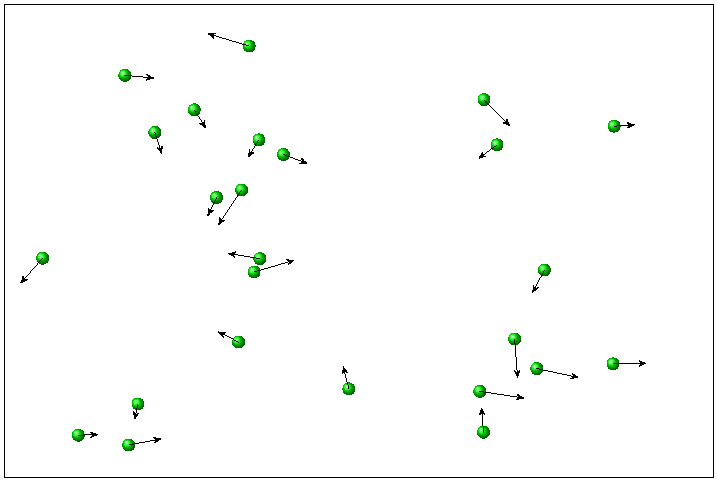
\includegraphics[width=6cm]{gas-random-motion}
		
	\caption{The motion of gas molecules in a container}
	
\end{marginfigure}

Our core assumption for ideal gasses is that a gas consists of a large number of molecules. These gas molecules move \emph{randomly} at high speeds and the  randomness results from \emph{collisions} of fast-moving molecules in the gas.

We assume that for an individual molecule, its velocity changes constantly as it collides with other molecules so at any instant, there is a range of molecule velocities.  

There is some strong evidence of random motion often referred to as \keypoint{Brownian motion}\footnote{We attribute the discovery of this random motion to the botanist Robert brown but there are many earlier descriptions from the early greeks - or this remarkable description of dust molecules from the roman Lucretius: \begin{quote}
    
``Observe what happens when sunbeams are admitted into a building and shed light on its shadowy places. You will see a multitude of tiny particles mingling in a multitude of ways... their dancing is an actual indication of underlying movements of matter that are hidden from our sight... It originates with the atoms which move of themselves [i.e., spontaneously]. Then those small compound bodies that are least removed from the impetus of the atoms are set in motion by the impact of their invisible blows and in turn cannon against slightly larger bodies. So the movement mounts up from the atoms and gradually emerges to the level of our senses so that those bodies are in motion that we see in sunbeams, moved by blows that remain invisible.''\end{quote}}\index{Brownian motion}. If you observe a dust mote or smoke particles in the air, you'll see that they undergo jerky random motion due to collisions with the randomly moving gas molecules. 

We know also from these observations that the speed of gas molecules depend on temperature, molecules move faster at higher temperature\footnote{We will prove this statement later in this chapter.}.

\subsection{Number of molecules}

In any tangible sample of gas, there are a huge number of molecules. We introduce the mole as a universally accepted \keypoint{amount of a substance}\index{amount of substance} to measure the size of a collection of particles.

\cmt unit of amount of substance: $[n] = \text{mol}$

\begin{ilight}
	One \keypoint{mole} is defined as the amount carbon-12 atoms in a sample of 12 grams. 1 mole of any substance contains 6.02$\times$10$^{23}$ particles
\end{ilight}

This number is called \keypoint{Avogadro constant}\index{Avogadro constant}: $N_A = 6.02\times10^{23} \text{ mol}^{-1}$ \footnote{In 2018, IUPAC suggested a new definition of the mole, which is defined to contain exactly 6.02$\times$10$^{23}$ particles. This new definition fixed numerical value of the Avogadro constant, and emphasized that the quantity `amount of substance' is concerned with counting number of particles rather than measuring the mass of a sample.}

With the constant being just a number, it's easy to convert between number of molecules and amount of substance: $\tcbhighmath{N=nN_A}$

One of the useful shortcuts that the mole grant us is the notion of molar mass $M$

\begin{ilight}
	\keypoint{Molar mass}\index{molar mass} of a substance is defined as the mass of a given sample divided by the amount of substance: $M=\frac{m}{n}$
\end{ilight}

\begin{compactitem}
	\item[--] $\text{amount of substance} = \frac{\text{mass of sample}}{\text{molar mass}}$, or $n = \frac{m}{M}$
	
	\eqyskip
	
	\item[--] $\text{mass of single molecule} = \frac{\text{molar mass}}{\text{Avogadro constant}}$, or $m_0 = \frac{M}{N_A}$
\end{compactitem}

	

\subsection{Pressure (qualitative view)}

When gas molecules collide with walls of container and rebound, they change their momentum. By Newton's second law there must be a force on them from the wall of the container. By Newton's third law, gas molecules must exert a reaction force on container. The contributions from many molecules give rise to a constant pressure.

\subsection{Empirical laws}

In 1643, the Italian physicist and mathematician, Evangelista Torricelli, who for a few months had acted as Galileo's secretary, conducted a celebrated experiment in Florence. He demonstrated that a column of mercury in an inverted tube can be supported by the pressure of air outside of the tube, with the creation of a small section of vacuum above the mercury. This experiment essentially paved the way towards the invention of the barometer, as well as drawing the attention of Robert Boyle, then a "skeptical" scientist working in England. Boyle was inspired by Torricelli's experiment to investigate how the elasticity of air responds to varying pressure, and he did this through a series of experiments performed by his assistant \emph{Robert Hooke}\footnote{Yes, that Hooke, of Hooke's law.}

\subsection*{Boyle's law}\index{Boyle's law}

Boyle's law was discovered by \emph{Robert Boyle} in 1662, based on experimental observations.

\begin{marginfigure}
	\centering
		\begin{tikzpicture}[yscale=1.2]
		\draw [thick, <->] (0,4) node[left]{$p$} -- (0,0) node[below]{$0$} -- (4,0) node[below]{$V$};
		\draw [very thick,blue,domain=0.28:3.6,samples=20,smooth,variable=\x] plot (\x,{1/\x)});
		\draw (2.5,2) node{$pV=\text{const}$};
		\end{tikzpicture}
  \caption{A $p$-$V$ relation for an isothermal process is shown.}
\end{marginfigure}

If temperature $T$ remains constant, then

{

\centering

$\tcbhighmath{pV=\text{const}}$, or $\tcbhighmath{p \propto \frac{1}{V}}$

} 

In other words, the pressure $p$ of a gas is inversely proportional to volume $V$ for a gas with fixed temperature: $p_1 V_1 = p_2 V_2$

A thermodynamic process for which temperature is kept constant is called an \emph{isothermal} process.

\subsection*{Charles's law}\index{Charles's law}

Charles's law was discovered by \emph{Jacques Charles} in 1787, based on experimental observations. Of the early laws it's a favourite, because of the huge concequences:

\begin{figure*}[ht]
	\centering
	\begin{tikzpicture}[scale=1.6]
		\draw [thick, ->] (-2.73,0.6) -- (-2.73,3) node[left]{$V$};
		\draw [thick, ->] (-3.2,0) -- (3,0) node[below]{$T_K/\text{K}$} node[above]{$T_C/\OC$};
		\draw [thick,blue,domain=-0.5:2.8,samples=2,smooth,variable=\x] plot (\x,{0.45*(\x+2.73)});
		\draw [thick,blue,dotted,domain=-2.73:-0.5,samples=2,smooth,variable=\x] plot (\x,{0.45*(\x+2.73)});
		\draw [thick,blue] (-0.5,1.0035) to [out=204.2,in=30] (-1.2,0.65) to [out=210,in=90] (-1.5,0.15);
		\draw[white,fill] (-2.3,0.2) rectangle (-1.8,0.5);
		\foreach \s in {-200,-100,...,200}
		\draw [thick] (\s/100,0) --(\s/100,0.1) node[above]{\s};
		\foreach \s in {0,100,...,500}
		\draw [thick] (\s/100-2.73,0) -- (\s/100-2.73,-0.1) node[below]{\s};
		\draw [thick] (-2.73,0) -- (-2.73,0.1) node[above]{-273};
		\draw [<-, thick] (-1.6,0.6) to [out=90, in=270] (-1,1.6) node[above]{ideal behaviour};
	\end{tikzpicture}
 \caption{Charles's Law - our first glimpse of Absolute zero.}
\end{figure*}

For a fixed pressure $p$, then: $\tcbhighmath{\frac{V}{T}=\text{const}}$, or $\tcbhighmath{V \propto T}$

In other words, the volume $V$ of gas is directly proportional to its temperature $T$. 

\cmt Note that proportionality relation only applies if Kelvin scale is used

A thermodynamic process for which pressure is kept constant is called an \emph{isobaric} process

% $V$-$T$ relation for an isobaric process is shown

\cmt Charles's law implies that volume of gas tends to zero at a certain temperature, this is how the idea of \emph{absolute zero} first arose. In reality of course as $T\to0$, a real gas condenses into solid and there will be deviation from ideal behaviour (dotted line).

\subsection*{Gay-Lussac's law}\index{Gay-Lussac's law}

\begin{figure*}
	\begin{tikzpicture}
		\draw[->](0,0) -- (10,0) node[anchor=north] {$T$C};
		\draw[->](8,-0.2) -- (8,5) node[anchor=west] {$P$};
		\draw[thick, red, dashed] (1,0) -- (8,3.0975);
		\draw[thick, red] (8,3.0975) -- (9.7,3.85);
		\draw (8.1,3.175) node[color=blue] {x};
		\draw (8.4,3.25) node[color=blue] {x};
		\draw (8.7,3.4) node[color=blue] {x};
		\draw (9.0,3.5) node[color=blue] {x};
		\draw (9.3,3.65) node[color=blue] {x};
		\draw (9.6,3.75) node[color=blue] {x};
		\draw[->] (1,-1) node[anchor=north]{Absolute Zero} -- (1,-0.2);
		\end{tikzpicture}
		\caption{Pressure against Temperature of a Gas}
\end{figure*}

Gay-Lussac's law was discovered by \emph{Joseph Louis Gay-Lussac} between 1800 and 1802. If volume $V$ remains constant, then

{
	
	\centering
	
	$\tcbhighmath{\frac{p}{T}=\text{const}}$, or $\tcbhighmath{p \propto T}$
	
} 

i.e., pressure $p$ is directly proportional to temperature $T$

\cmt \piste A thermodynamic process for which volume is kept constant is called an \emph{isochoric} process, or \emph{isometric} process

The $p$-$T$ relation for an isochoric process is shown and whilst it also predicts Absolute Zero we would again expect the real behaviour to  deviate from ideal behaviour (dotted line) as $T\to0$

\section{Avogadro's Law}

This is the law commonly overlooked in textbooks - or at least, not overtly stated. 
\begin{ilight}
    Avogadro's law states that ``equal volumes of all gases, at the same temperature and pressure, have the same number of molecules.''
\end{ilight}
For a given mass of an ideal gas, the volume and amount (moles) of the gas are directly proportional if the temperature and pressure are constant.
$$\frac{V}{n}=k$$
Where
$V=$ Volume of the gas
$n=$ Amount of substance (usually in moles)
$k=$ Constant. If $n$ is in moles, this is the molar gas constant.

\subsection{An ideal gas}

With the above realationships we can build a universal pressure-temperature-volume-stuff equation sufficient to model the behaviour of real gasses. The assumptions of an ideal gas however are: 
\begin{itemize}
    \item An ideal gas is made up of numerous identical point-like molecules, spread really far apart so that the intermolecular forces are negligible;
\item Ideal gas molecules undergo random motion and obey Newton's laws of motion;
\item Ideal gas molecules undergo elastic collisions with the walls of the container the gas is in;
\item Ideal gas molecules experience only completely elastic collisions with one another.

\end{itemize}
\subsection{The ideal gas equation}

The ideal gas law was first stated by \emph{\'Emile Clapeyron} in 1834:

for a fixed amount of gas, $\tcbhighmath{\frac{PV}{T} = \text{const}}$

His work was based on the empirical Boyle's law, Charles's law, Avogadro's Law and Gay-Lussac's law

\begin{ilight}
	A gas that satisfies the equation $\tcbhighmath{pV=nRT}$ or $\tcbhighmath{pV=NkT}$ at any pressure $p$, any volume $V$, and thermodynamic temperature $T$ is called an \keypoint{ideal gas}\index{ideal gas}.
\end{ilight}

\keypoint{Molar gas constant}: $R=8.31 \text{ J mol}^{-1}\text{ K}^{-1}$

\keypoint{Boltzmann constant}: $k=1.38\times10^{-23} \text{ J K}^{-1}$

The Values of $R$ and $k$ apply for any ideal gas, i.e., they are \emph{universal} constants.

Recall conversion between number of molecules and amount of substance: $$\tcbhighmath{N=nN_A}$$

so we have a relation between the constants: $R = kN_A$, or $k=\frac{R}{N_A}$

Note that one should use \emph{thermodynamic temperature} in the equations. We can often get away with centigrade or celcius as we're usually talking about a \emph{change in temperature} and the steps are about the same size.

Thermodynamic temperature is measured in kelvins (K), so it is also called the \emph{Kelvin scale}\footnote{We will discuss in details about Kelvin scale in \S\ref{s-temp-scale} and \S\ref{s-abs-zero}.}

To convert between Kelvin temperature and Celsius temperature: $\tcbhighmath{T_K (\text{K}) \text{ } \autorightleftharpoons{\footnotesize -273}{\footnotesize +273} \text{ } T_C (\OC)}$

\subsection*{Real gases}

We always treat gasses as ideal, and indeed, real gasses behave ideally at sufficiently high temperature and low pressure.

\begin{compactitem}
	\item[--] at very low temperatures, a real gas will condense into liquid or solid.
	
	\item[--] at very high pressures, intermolecular forces become important.
\end{compactitem}

however, under normal conditions (room temperature $T \approx 300 \text{ K}$ and standard atmospheric pressure $p \approx 1.0\times10^5 \text{ Pa}$), there is no significant difference between a real gas and an ideal gas so the ideal gas approximation can be used with good accuracy for most of our applications.

\newpage %%%%

. The pressure of this air is $2.8\times10^5 \text{ Pa}$ at a temperature of $25^\circ$C. The pressure is to be increased using a pump. On each stroke 0.015 mol of air is forced into the tyre. If gas has a final pressure of $3.6\times10^5 \text{ Pa}$ and final temperature of $28^\circ$C. Find the number of strokes of the pump required.

\subsection{The kinetic theory of ideal gases}

\keypoint{Kinetic model of gases}\index{kinetic model of gases}: a theory based on microscopic motion of molecules of a gas that explains its macroscopic properties

\subsection{Assumptions of ideal gas model}

\begin{ilight}
	
kinetic theory of the ideal gas model is based on the following assumptions:

\begin{compactitem}
	
\item[--] gas molecules are in constant \emph{random} motion
	
\item[--] \emph{intermolecular separation} is much greater than size of molecules

volume of molecules is negligible compared to volume occupied by gas

\item[--] \emph{intermolecular forces} are negligible

\item[--] collisions between molecules are perfectly \emph{elastic}, i.e., no kinetic energy lost

\item[--] molecules travel in straight line between collisions
\end{compactitem}

\end{ilight}

\subsection{Pressure (quantitative view)}

The pressure of gas on a container is due to collision of gas molecules with container. To derive an expression for this, let's first consider the effect of one single molecule moving in one dimension only, and then generalise the result to a gas containing $N$ molecules moving in all three dimensions.

\begin{figure}[ht]
\centering
\begin{tikzpicture}[scale=1]
\coordinate (A) at (0,0); 
\coordinate (B) at (3,0);
\coordinate (C) at (4.5,1); 
\coordinate (D) at (1.5,1);
\coordinate (E) at (0,3); 
\coordinate (F) at (3,3);
\coordinate (G) at (4.5,4); 
\coordinate (H) at (1.5,4);
\draw [gray!20,fill] (A) -- (D) -- (H) -- (E) -- cycle;
\draw [thick] (B) -- (A) -- (E) -- (F) -- (B) -- (C) -- (G) -- (H) -- (E);
\draw [thick] (F) -- (G);
\draw [thick,dashed] (A) -- (D) -- (C);
\draw [thick,dashed] (D) -- (H);
\draw [thick,blue,->] (1.6,2.1) -- (0.9,2.1) to [out=180,in=90] (0.75,1.95)to [out=-90,in=180] (0.9,1.8) -- (2.4,1.8) node[below, pos=0.7]{$v$};
\shade [ball color = green] (1.8,2.1) circle [radius=0.1];
\draw [thick,<->] (0,-0.5) -- (1.5,-0.5) node[below]{$l$} -- (3,-0.5);
\node at (0.75,2.5) {{\Large $A$}};
\node[above] at (1.8,2.2) {{\footnotesize $m$}};
\end{tikzpicture}

\caption{One gas molecule moving in 1-D}
\label{onedmol}
\end{figure}

Let's assume this single molecule only moves in $x$-direction (see figure \ref{onedmol}). The change in momentum when colliding with wall: $\Delta P_x = mv_x - (-mv_x) = 2mv_x$\footnote{In this chapter we use $P$ for momentum of a particle and $p$ for pressure of a gas to avoid confusion.}

The time interval between collisions: $\Delta t=\frac{2l}{v_x}$

So the average force: $F_x=\frac{\Delta P_x}{\Delta t} = \frac{2mv_x}{\tfrac{2l}{v_x}} = \frac{mv_x^2}{l}$

aWhich in turn leads to the average pressure: $p_x=\frac{F}{A} = \frac{mv_x^2}{lA} = \RA p_x = \frac{mv_x^2}{V}$

We finally need to generalise to $N$ molecules moving in 3-D;

\begin{compactitem}
	\item[--] $N$ molecules so $N$ times the contributions to pressure
	
	but there is a \emph{distribution} of speeds for $N$ molecules, so should take average of $v^2$
	
	\item[--] in three-dimensional space, we have: $v^2=v_x^2 + v_y^2 + v_z^2$
	
	but molecules have no preference in any specific direction, so: $\avg{v_x^2} = \avg{v_y^2} = \avg{v_z^2} = \frac{\avg{v^2}}{3}$
	
	pressure should be shared equally among three dimensions: $p=p_x=p_y=p_z$
		
\end{compactitem}

therefore we find the pressure of an ideal gas is given by: $$\tcbhighmath{p = \frac{Nm\avg{v^2}}{3V}}$$

\cmt Where $\avg{v^2}$ is the \emph{mean square velocity} of gas molecules.

we can further define r.m.s. (root mean square) velocity: $v_\text{rms} = \sqrt{\avg{v^2}}$ .

Note that the gas molecules in random motion so there exists a range of velocities. We have to treat the molecules statistically - in other words, we cannot tell exact velocity of a specific molecule, but can only tell mean values.

\cmt If $N$ is number of molecules, and $m$ is mass of one molecule then $Nm$ gives total mass of the gas, and $\frac{Nm}{V}$ gives gas density $\rho$

we can rewrite the pressure formula as: $$\tcbhighmath{p=\frac{1}{3}\rho \avg{v^2}}$$ 

This shows clearly that pressure depends only on density and mean square speed of molecules and leads to some useful conclusions:
\begin{compactitem}
\item[--] $N \up$ $\ra$ more molecules, more collisions $\ra p\up$

\item[--] $m \up$ $\ra$ greater mass, greater force upon collision $\ra p\up$

\item[--] $v \up$ $\ra$ strike container harder, also more often $\ra p\up$

\item[--] $V \up$ $\ra$ spend more time in gas, less frequent collision with container $\ra p\down$
\end{compactitem}

\subsection{Kinetic energy of a gas}

We have assembled two equations for ideal gases:
\begin{equation*}
\left\{
	\begin{array}{ll}
	pV = nRT \, \text{, or } \, pV = NkT &\quad \text{ideal gas law} \\
	p = \frac{Nm\avg{v^2}}{3V} &\quad \text{pressure law}
	\end{array} \right.
\end{equation*}

If we compare the two equations: $$pV=\frac{1}{3}Nm\avg{v^2}=NkT \RA m\avg{v^2}=3kT$$

It becomes clear that we have an expression for the \emph{mean kinetic energy} of a single molecule in a gas: $$\tcbhighmath{\avg{E_k}=\frac{1}{2}m\avg{v^2}=\frac{3}{2}kT}$$

This mean K.E. of ideal gas molecules is \emph{proportional} to its thermodynamic temperature - it can be helpful to think about the link with molecular speeds: $\tcbhighmath{v_\text{rms}^2 \propto T}$

Recall that a higher temperature means higher speed for molecules but we only talk about \emph{translational} K.E. here - molecules have this energy because they are moving through space. The total kinetic energy may also include \emph{rotational} K.E. and \emph{vibrational} K.E.
\footnote{There is an important result in classical thermal physics, known as the \emph{equipartition of energy theorem}. It states that the average energy per molecule is $\frac{1}{2}kT$ for each independent \emph{degree of freedom}. A molecule can move in three directions, corresponding to three translational degrees of freedom, thus its mean translational kinetic energy is $\frac{3}{2}kT$. For a polyatomic gas (each molecule consists of several atoms), apart from translational motion , it has additional rotational degrees of freedom and different vibrational modes, so its average energy can be calculated by counting the total number of degrees of freedom.}

$$\avg{E_k} = \frac{3}{2}k T$$ gives the \emph{mean}, or \emph{average} K.E. per molecule. The gas molecules exchange energies with each other upon collisions so for any individual molecule, the K.E. is not a constant. The mean K.E. however is constant, which depends on temperature $T$ only. In a mixture of several gases, K.E. is shared \emph{equally} among its components because of repeated collisions between particles. What this means in practive is that all molecules have same K.E., so heavier molecules will move more slowly.

\cleardoublepage

% ===== Chapter: 22-thermal-physics =====
\chapter{Thermodynamics}

\subsection{Thermal physics basics}

\subsection{Temperature scales}\label{s-temp-scale}

\begin{marginfigure}
	\centering
	\vspace*{-2.7cm}
	\begin{tikzpicture}[yscale=1.6]
	\draw[->] (0,-3) -- (0,1.50);
	\foreach \temp in {-2.73,-1.96,0,0.25,1.00} \draw (-0.1,\temp) --++ (0.2,0);
	\node[left] at (-0.2,1.5) {$T_C(\OC)$};
	\node[right] at (0.2,1.5) {$T_K(\text{K})$};
	\node[left] at (-0.2,-2.73) {-273\OC};
	\node[left] at (-0.2,-1.96) {-196\OC};
	\node[left] at (-0.2,-0) {0\OC};
	\node[left] at (-0.2,0.25) {25\OC};
	\node[left] at (-0.2,1) {100\OC};
	\node[right] at (0.2,-2.73) {0 K};
	\node[right] at (0.2,-1.96) {77 K};
	\node[right] at (0.2,-0) {273 K};
	\node[right] at (0.2,0.25) {298 K};
	\node[right] at (0.2,1) {373 K};
	\node[right] at (1.35,-2.73) {absolute zero};
	\node[right] at (1.35,-1.96) {liquid nitrogen};
	\node[right] at (1.35,0) {ice-water mixture};
	\node[right] at (1.35,0.25) {room temperature};
	\node[right] at (1.35,1.00) {boilng water};
	\end{tikzpicture}
	\vspace*{-30pt}
\end{marginfigure}
There are a few scales that you might come across - in fact we have met them already. 
\cmt Celsius scale (unit: \OC)
0$^\circ$C defined as temperature of ice-water mixture
100$^\circ$C defined as temperature of boiling water

\cmt Kelvin scale (unit: K)
0 K (\emph{absolute zero}) is lowest temperature possible

\cmt Conversion rule: $T_K (\text{K}) \text{ } \autorightleftharpoons{\footnotesize -273}{\footnotesize +273} \text{ } T_C (\OC)$

\cmt Change of 1$^\circ$C equals change of 1 K

\subsection{The kinetic theory of matter}

There are three common states of matter: solid, liquid and gas, they have very different physical properties (density, compressibility, fluidity, etc.) but deep down, they are all composed of a large number of small molecules. In the \keypoint{kinetic theory of matter}, we look at microscopic behaviour at molecular level (arrangement, motion, intermolecular forces, separation, etc.). The \emph{microscopic} behaviour of molecules causes differences in \emph{macroscopic} properties of matter.

\begin{compactitem}
	\item[--] solid: molecules close together, tightly bonded, vibrate about their positions
	
	\item[--] liquid: molecules quite close together, vibrate but has some freedom to move about
	
	\item[--] gas: molecules widely separated, free from neighbours, move rapidly
\end{compactitem}

\subsection{Specific latent heat}

Changing state requires a change in the energy stored by a material. It requires heat energy to \emph{melt} a solid or \emph{boil} a liquid. Melting and boiling usually occur at a fixed temperature. The thermal energy to cause the change of state at a constant temperature is called \emph{latent heat}

The amount of latent heat needed depends on mass of substance: $\tcbhighmath{Q=Lm}$

\begin{ilight}
	We define \keypoint{specific latent heat}\index{specific latent heat} ($L$) as the thermal energy required to change the state of \emph{unit} mass of substance with no change in temperature.
\end{ilight}

\cmt unit of specific latent heat: $[L] = \text{J}\cdot\text{kg}^{-1}$

The specific latent heat, $L$, does not depend on size or shape of sample, $L$ depends on type of substance only. For melting, $L$ is called \emph{specific latent heat of fusion}. For boiling, $L$ is called \emph{specific latent heat of vaporisation}.
Latent heat is related to breaking bonds and increasing intermolecular separation, vaporisation requires larger increase in particle separation than fusion so for any given substance: $L_\text{vapour}>L_\text{fuse}$

	

 

\begin{center}
	\begin{tabular}{|C{1.6cm}|C{2cm}|c|c|}
		\hline  & Power (W) & time interval (min) & mass of ice melted (g) \\ 
		\hline test 1 & 60 & 3.0 & 40.4 \\ 
		\hline test 2 & 90 & 3.0 & 56.6 \\ 
		\hline 
	\end{tabular} 
\end{center}

\subsection{Specific heat capacity}

Heating a substance, in addition to melting or vapourising it, is likely to cause an increase in its temperature. The heat required is proportional to its mass $m$ and temperature change $\Delta T$: $\tcbhighmath{Q=cm\Delta T}$

\begin{ilight}
	We define \keypoint{specific heat capacity }\index{specific heat capacity} ($c$) as the thermal energy required per unit mass of substance to cause an increase of one unit in its temperature.
\end{ilight}

\cmt unit of specific heat capacity: $[c] = \text{J kg}^{-1} \text{ K}^{-1}$ or J kg$^{-1}$ $^\circ\text{C}^{-1}$
	
$c$ is also independent of the size or shape of the sample.

\begin{fullwidth}
    

\end{fullwidth}

\begin{figure}[ht]
	\centering
	\begin{tikzpicture}[scale=1]
	\draw[style=help lines,step=0.5,gray!50] (0,0) grid (7.5,5.5);
	\draw [thick, ->] (-0.5,0) --(8,0) node[below]{$t/\text{s}$};
	\draw [thick, ->] (0,-0.5) --(0,6) node[left]{$T/\OC$};
	\foreach \s in {100,200,...,700}
	\draw [very thick] (\s/100,-0.1) -- (\s/100,0) node[below]{\s} -- (\s/100,0.1);
	\foreach \s in {10,20,...,50}
	\draw [very thick] (-0.1,\s/10) -- (0,\s/10) node[left]{\s} -- (0.1,\s/10);
	\draw [very thick,blue] (0,2) -- (7.5,5.075);
	\draw [very thick,red] (0,2) -- (5.5,2) node[midway,below]{\textcolor{black}{$\Delta t = 550 \text{ s}$}} -- (5.5,4.255) node[right,midway]{\textcolor{black}{$\Delta T = 22.5 \OC$}};
	\foreach \s in {0,1,...,7}
	\draw [fill] (\s,2+0.41*\s) circle(0.05);
	\end{tikzpicture}
\end{figure}

\begin{center}
	\begin{tabular}{|l|c|c|}
		\hline  & silver & gold \\ 
		\hline melting point (K) & 1240 & 1340 \\ 
		\hline specific heat capacity (solid or liquid) (J kg$^{-1}$ K$^{-1}$) & 235 & 129 \\ 
		\hline specific latent heat of fusion (kJ kg$^{-1}$) & 105 & 628 \\
		\hline 
	\end{tabular} 
\end{center}

\subsection{Internal energy}

We now consider the total energy within a thermodynamic system, molecules in a system undergo random motion, so they have kinetic energy. They must also have potential energy between molecules due to intermolecular interaction.

\begin{ilight}
	\keypoint{internal energy}\index{internal energy} is defined as the sum of random kinetic energy of molecules and potential energy between molecules: $\tcbhighmath{U=E_k+E_p}$
\end{ilight}

Internal energy is a \emph{state function} of the system - it only depends on current state of system, not on whatever process occurred to arrive at this state.

\subsection{Kinetic energy}

Internal energy counts K.E. due to random motion at molecular level - the K.E. of macroscopic motion of the system as a whole is not included.

\cmt mean K.E. of molecules is directly proportional to temperature: $\tcbhighmath{E_k \propto T}$

K.E. of molecules depends on temperature only, higher temperature means molecules move faster, vibrate more intensively, etc.

\subsection{Potential energy}

The internal energy counts P.E. due to force fields \emph{within} the system, the P.E. of the system as a whole due to \emph{external} force fields is not included.

\cmt P.E. between molecules depends on intermolecular separation and chemical bonding

in general, greater intermolecular separation means greater P.E.\footnote{Intermolecular separation does not necessarily increase during melting processes. A typical counter example is melting of ice into water, for which intermolecular separation actually decreases (density of water > density of ice), but potential energy of the system will still increase because hydrogen bonds between H$_2$O molecules are broken.}: $$\tcbhighmath{r \up \Leftarrow E_p \up}$$

Breaking intermolecular bonds also causes an increase in P.E.

mean P.E. of gas $>$ mean P.E. of liquid $>$ mean P.E. of liquid solid

\subsection{Internal energy of ideal gas}

For ideal gas, mean K.E. of one molecule: $E_k = \frac{3}{2}kT$

From our assumptions - there is no intermolecular force, so P.E. of ideal gas is defined to be zero: $E_p = 0$.

Internal energy per molecule: $U = E_k + E_p = \frac{3}{2}kT$ and hence internal energy of ideal gas is purely kinetic and directly proportional to temperature. 

The total internal energy of the gas: $U_\text{gas} = NU \RA \tcbhighmath{U_\text{gas} = \frac{3}{2}NkT}$

\subsection{Change of states}

Consider a substance being heated from its solid state, it will melt into a liquid and further vaporise into its gaseous state, we now look into the changes of internal energy during each stage.

\begin{figure}[ht]
\centering
\begin{tikzpicture}[scale=1]
\draw[thick,->] (-1,-2) -- (0,-2) -- (10,-2) node[below] {$t$};
\draw[thick,->] (0,-2.5) -- (0,5) node[left]{$T$};
\draw [very thick,blue] (0,-1) node[left]{$A$} -- (1,0) node[above]{$B$} -- (2.5,0) node[above left]{$C$} -- (4,3) node[above]{$D$} -- (9,3) node[above left]{$E$} -- (9.5,4.5) node[above]{$F$};
\draw[thick,dashed] (4,3) -- (0,3) node[left]{$T_\text{boiling}$};
\draw[thick,dashed] (1,0) -- (0,0) node[left]{$T_\text{melting}$};
\end{tikzpicture}
\end{figure}

\begin{compactitem}
\item[--] $AB$ (solid state): $T \up \ra E_k \up$, greater vibration for solid particles

but no (significant) change in mean separation\footnote{A typical solid material expands when it is heated, so intermolecular separation will increase slightly.} $\ra$ no change in P.E.

\item[--] $BC$ (\emph{melting}): latent heat goes into breaking intermolecular bonds, $r\up \ra E_p \up$

but melting occurs at constant temperature\footnote{Here we talk about \emph{pure substance}, which changes from solid into liquid at a particular temperature, called the \emph{melting point}. But for a \emph{mixture} of substances, melting may occur over a \emph{range} of temperatures. It is also possible for a substance to decompose before they change states.} $\ra$ no change in K.E.

\item[--] $CD$ (liquid state): $T \up \ra E_k \up$, greater vibration and free motion

but no (significant) change in mean separation $\ra$ no change in P.E.

\item[--] $DE$ (\emph{boiling}): molecules break free, $r\up \ra E_p \up$

boiling occurs at constant temperature\footnote{Again we only concern pure substances. Mixtures that boil over a range of temperatures or substance decompose before phase transition are not considered here.} $\ra$ no change in K.E.

\item[--] $EF$ (gas state): $T \up \ra E_k \up$ particles move even faster

particles completely separated, no intermolecular force, so constant $E_p = 0$
\end{compactitem}

\subsection*{Evaporation}

liquid changes into gas without boiling $\longrightarrow$ \keypoint{evaporation}

particles move randomly, i.e., they move at various speeds

some molecules move fast enough to break free

\cmt \emph{cooling effect}: evaporation causes a decrease in temperature of the liquid

most energetic molecules escaped, those remain in the liquid have less energy, $E_k \down \ra T \down$

\cmt rate of evaporation increases with temperature, surface area of liquid

\cmt different between boiling and evaporation

\begin{center}
	\begin{tabular}{|c|c|c|}
		\hline 
		& boiling & evaporation \\ 
		\hline 
		occurrence & throughout the liquid & at surface only \\ 
		\hline 
		temperature & occur at boiling point & occur at any temperature \\ 
		\hline 
		bubble formation & bubbles formed & no bubbles \\ 
		\hline 
		rate of process & fast & slow \\ 
		\hline 
	\end{tabular} 
\end{center}

\subsection{First law of thermodynamics}

internal energy of a system changes upon heat transfer or doing work

\begin{ilight}
	\keypoint{first law of thermodynamics}\index{law of thermodynamics!first law of thermodynamics} states that the increase in internal energy equals sum of heat supply to the system and work done on the system: $\tcbhighmath{\Delta U = Q +  W}$
\end{ilight}

\cmt first law of thermodynamics is an extension of the law of conservation of energy

\cmt sign conventions for $Q$ and $W$

\begin{compactitem}
	\item[$\circ$] $Q>0$ if heat supplied to system
	
	\item[$\circ$] $Q<0$ if heat released by system to surroundings
	
	\item[$\circ$] $W>0$ if work done \emph{on} system by external
	
	i.e., if system is compressed and volume decreases, then $W>0$
	
	\item[$\circ$] $W<0$ if system does work \emph{against} surroundings
	
	i.e., system expands and volume increases, then $W<0$
	
\end{compactitem}

\cmt amount of heat energy: $Q=\left\{ \begin{array}{l}
	cm\Delta T \qquad (\text{if no change of state}) \\
	Lm \qquad (\text{during change of state})
	\end{array}\right.$

\cmt amount of work is related to pressure and change of volume

if volume changed at \emph{constant} pressure, then $W=F\Delta s = pA\Delta s \ra \tcbhighmath{W = p\Delta V}$\footnote{If pressure changes with volume during a thermodynamics process, then work done $W=\int p \dd V$. Alternatively, we can evaluate the area under a $p$-$V$ graph to find the work done.}

if no change of volume, then no work is done

\begin{figure}[h]
		\begin{tikzpicture}[domain=1:9]
		\draw[->] (-0.5,0) -- (12,0) node[anchor=north] {$V$};
		\draw[->] (0,-0.5) -- (0,10) node[anchor=east] {$P$};
		\draw (1,9) node[anchor=south]  {\textbf{A}};
		\draw[thick, ->]  (1,9) .. controls (4,7) and (7,6.2) .. (8,6) node[midway, anchor=south west] {\textbf{1}};
		\draw[thick, ->] (8,6) .. controls (9,4.5) and (10,3) .. (12,1) node[anchor=south west, midway] {\textbf{2}};
		\draw[thick, ->] (12,1) .. controls (8,1.5)  .. (3,3) node[midway, anchor=north east] {\textbf{3}};
		\draw[thick, ->] (3,3) .. controls (1.6,6)  .. (1,9) node[midway, anchor=north east] {\textbf{4}};
		\end{tikzpicture}
		\caption{The Carnot Cycle}
		\label{carnotcycle}
	\end{figure}
 
The Carnot Cycle shown in Figure \ref{carnotcycle} is commonly used to test the understanding for the first law. The cycle begins and ends at point \textbf{A}. This means that the internal energy of the system at the start and end of the cycle is the same (as $PV=nRT$ and $T$ is proportional to the internal energy). The changes at each stage of the cycle are as follows:
	
	\begin{description}
		\item[1. Isothermal Expansion] In stage 1 the gas expands at contant temperature. Since it is expanding, the gas is doing work on the surroundings and since it is at constant temperature the internal energy of the gas remains constant. Therefore the second law implies that the gas must be absorbing heat. \emph{Note that isothermal changes are often indicated by describing the change as occuring slowly.}
		\item[2. Adiabatic Expansion] In stage 2 the gas expands without transferring heat to/from the surroundings. Since it is doing work the gas's internal energy drops, as does its temperature.
		\item[3. Isothermal Compression] In stage 3 the gas is compressed at constant temperature. Since work is done on the gas and the internal energy remains constant it must be the case that heat is lost to the surroundings.
		\item[4. Adiabatic Compression] Finally, the gas is compressed without heat transfer to/from the surroundings. Work is done on the gas and therefore the internal energy, and termperature, increase.
	\end{description}
	
	
	\begin{example}
		
		Complete the table for the Carnot Cycle shown in figure \ref{carnotcycle}.
		
		\begin{tabular}{|c|p{3cm}|p{3cm}|p{3cm}|}
			\hline
			stage & \centering thermal energy supplied \textbf{to} the gas / J & \centering work done \textbf{on} the gas / J & \centering \textbf{increase} in internal energy of the gas / J \tabularnewline \hline
			1 & \centering\centering(a) & \centering-936 & \centering(b) \tabularnewline \hline
			2 & \centering0 & \centering(c) & \centering(d) \tabularnewline \hline
			3 & \centering(e) & \centering+702 & \centering0 \tabularnewline \hline
			4 & \centering(f) & \centering+844 & \centering+844 \tabularnewline \hline
		\end{tabular}
		
		
		
		In stage 1 there is no change in internal energy of the gas, so (b) equals zero. In order to satisfy the first law of thermodynamics the thermal energy supplied must equal the work done \textbf{by} the gas so (a) equals +936J.
		
		As the total change in internal energy throughout the cycle must be zero, we can now calculate (d) as being -844J.
		
		(c) can be calculated using the first law as -844J.
		
		A similar argument to that used in stage 1 can be used in stage 3 to give (e) as -702J.
		
		In stage 4 no energy is transferred by heating therefore (f) is equal to zero.
		
		
		
		The final table is therefore:
		
		\begin{tabular}{|c|p{3cm}|p{3cm}|p{3cm}|}
			\hline
			stage & \centering thermal energy supplied \textbf{to} the gas / J & \centering work done \textbf{on} the gas / J & \centering \textbf{increase} in internal energy of the gas / J \tabularnewline \hline
			1 & \centering\centering \textbf{+936} & \centering-936 & \centering \textbf{0} \tabularnewline \hline
			2 & \centering0 & \centering \textbf{-844} & \centering \textbf{-844} \tabularnewline \hline
			3 & \centering \textbf{-702} & \centering+702 & \centering0 \tabularnewline \hline
			4 & \centering \textbf{0} & \centering+844 & \centering+844 \tabularnewline \hline
		\end{tabular}
		
	\end{example} 

\begin{figure}[ht]
	\centering
	\begin{tikzpicture}[scale=0.9]
	\draw[<->] (0,7.5) node[left]{$p$/kPa} -- (0,0) -- (7.5,0) node[below] {$V/10^{-2}$ m$^3$};
	\draw[help lines, gray] (0,0) grid (7,7);
	\foreach \x in {0,100,200,300} \node[left] at (-0.1,\x*2/100) {$\x$};
	\foreach \x in {0,2,4,6} \node[below] at (\x,-0.1) {$\x$};
	\draw[very thick, blue, ->] (2,2) node[below left]{$A$} -- (2,4.5);
	\draw[very thick, blue] (2,4.5) -- (2,6) node[above left]{$B$};
	\draw [very thick, blue, domain=2:6] plot (\x, {12/\x}) node[below right]{$C$};
	\draw[very thick, blue, ->] (6,2) -- (3.5,2);
	\draw[very thick, blue] (3.5,2) -- (2,2);
	\draw[very thick, blue, ->] (4.5,2.67) -- (4.55,2.64);
	\end{tikzpicture}
\end{figure}

Temperature of state $A$ is 300 K. The magnitude of work on gas from state $B$ to $C$ is 6570 J.

For each stage $A \to B$, $B \to C$ and $C \to A$ during the cycle, determine work done and heat supply to the gas, and also find the change in internal energy.

\newpage

\subsection{Temperature}

\subsection{Temperature \& thermal energy}

Temperature can be considered as a \emph{relative} measure of thermal energy, temperature can tell us the \emph{direction} of thermal energy flow because heat always (spontaneously) flows from high temperature regions to colder regions\footnote{This is the consequence of the \emph{second law of thermodynamics}\index{law of thermodynamics!second law of thermodynamics \piste}, which is concerned with the direction of natural processes. The law states that the total \emph{entropy}, a quantity that counts the number of microstates of a system, of an isolated system can never decrease over time. You will learn more about entropy if you study A-Level chemistry.}

If two objects in contact have the same temperature, then there is no net heat transfer and the two objects are said to be in \keypoint{thermal equilibrium}\index{thermal equilibrium}.

If two systems $A$ and $B$ are each in thermal equilibrium with a third system $C$, $A$ and $B$ are also in thermal equilibrium, this is called the \keypoint{zeroth law of thermodynamics}\index{law of thermodynamics!zeroth law of thermodynamics}
\footnote{This law is important for the formulation of thermal physics. The physical meaning of the law was expressed by Maxwell: "All heat is of the same kind." The zeroth law allows us to give the mathematical definition of temperature.}

\subsection{Absolute zero}\label{s-abs-zero}

We have met this concept in several places. From a thermodynamics point of view, the mean K.E. of molecules is a microscopic description of temperature $T$ so the minimum K.E. occurs if molecules do not move at all (completely frozen)\footnote{In the \emph{classical} description, there is no reason not allowing a molecule to cease motion. However, due to \emph{quantum mechanical effects}, kinetic energy of a system cannot be zero even at absolute zero.}.

The lack of any motion corresponds to the lowest possible temperature, called \keypoint{absolute zero}\index{absolute zero}.

\keypoint{Kelvin scale of thermodynamic temperature} is defined based on absolute zero as 0 K\footnote{More precisely, 0 K for absolute zero  and $273.16\text{ K}$ for water triple point.}

\cmt The conversion rule between Celsius scale and Kelvin scale\footnote{The numerical value of 273.15 will only be quoted in this chapter. For everywhere else in the notes, we will use the less precise value 273 for simplicity.}: $$\tcbhighmath{T_K (\text{K}) \text{ } \autorightleftharpoons{\footnotesize -273.15}{\footnotesize +273.15} \text{ } T_C (\OC)}$$

\cmt Kelvin scale is said to be an \emph{absolute scale} - zero of Kelvin scale does not depend on property of a specific substance, in contrast, zero of Celsius scale is based on properties of water. Theoretically it is impossible to remove any more energy from a system at 0 K (or -273.15 \OC) but there is no practicable means to bring a physical system to exactly $0\text{ K}$. The closest anone has got (at time of writing is (MIT) where physicists successfully cooled molecules in a gas of sodium potassium to a temperature of 500 nanokelvins. 
\footnote{This is known as the \emph{third law of thermodynamics}\index{law of thermodynamics!third law of thermodynamics \piste}, which states that it is impossible, no matter how idealized, to reduce the temperature of any closed system to absolute zero in a finite number of operations.}

\subsection{Thermometer}

T \keypoint{thermometer}\index{thermometer} is a device which can be used to measure temperature

\subsection*{Liquid-in-glass thermometer}

Basic principle: liquid expands in volume at higher temperature, examples include alcohol thermometer, mercury-in-glass thermometer, etc.

\begin{center}
	\begin{tikzpicture}[scale=1.35]
		\draw[red!50,fill] (45:0.6) arc(45:315:0.6) [out=45, in=180] to (0.8,-0.3) -- (4,-0.3) -- (4,0.3) -- (0.8,0.3) [out=180, in=-45] to (45:0.6);
		\draw[ultra thick] (45:0.6) arc(45:315:0.6) [out=45, in=180] to (0.8,-0.3) -- (8,-0.3) arc(-90:90:0.3) -- (0.8,0.3) [out=180, in=-45] to (45:0.6);
		\draw[thick] (1,0) -- (7.67,0);
		\foreach \temp in {0,10,20,...,100}{
			\draw[thick] (1+\temp/15,-0.15) --++ (0,0.3);
			\node[below] at (1+\temp/15,-0.3) {{\scriptsize \temp\OC}};
		}
	\end{tikzpicture}
\end{center}

\subsection*{Resistance temperature detectors (RTD)}

Basic principle: resistance of electronic element changes with temperature - metal wires and thermistor are both used in RTD elements.

\subsection*{Thermocouple}\index{thermocouple}

Basic principle: difference in temperature can produce a \emph{thermoelectric voltage} across junctions, thermocouple measures temperatures by means of this voltage

\begin{figure}[ht]
	\centering
	\begin{tikzpicture}
		% temp region boxes
		\draw[dashed,fill=gray!10] (-6,-1) rectangle (-4,1);
		\node at (-5.4,0.5) {$T_m$};
		\draw[dashed,fill=gray!10] (-1,-2) rectangle (1,2);
		\node at (0,1.6) {$T_\text{ref}$};
		% wires and junctions
		\draw[ultra thick,purple] (-5,0) [out=30,in=180] to (0,1);
		\node at (-2.5,1.25) {metal $A$};
		\node at (-2.5,-1.25) {metal $B$};
		\draw[ultra thick,Green] (-5,0) [out=-30,in=180] to (0,-1);
		\draw[fill] (-5,0) circle(0.1);
		\draw[fill] (0,1) circle(0.1);
		\draw[fill] (0,-1) circle(0.1);
		% connection to voltmeter
		\draw[thick] (0,1) --++ (3,0) --++ (0,-2) -- (0,-1);
		\draw[fill=white] (3,0) circle(0.4) node {V};
	\end{tikzpicture}
	
	\caption{typical configuration of a thermocouple unit}
\end{figure}

two pieces of different metal wires are joined at their ends

if there exists a temperature difference between the ends, a \emph{thermoelectric voltage} is developed

this voltage depends on temperature difference, captured by some characteristic function

in practice, we place the \emph{measurement} junction in an environment of unknown temperature

the other end, or the \emph{reference} junction, is at a known temperature

temperature difference is deduced from the voltage reading

hence the desired temperature can be determined

\vspace*{\baselineskip}

\cmt features of a thermometer:
\begin{compactitem}
	\item[--] \emph{range}: whether the thermometer can measure very low or very high temperatures
	
	\item[--] \emph{sensitivity}: whether a small change in temperature can be detected
	
	\item[--] \emph{response time}: whether changes in temperature can be immediately measured
	
	\item[--] \emph{linearity}: whether changes in temperature are proportional to changes in output
	
\end{compactitem}

%\cmt any thermometer requires \emph{calibration}
%
%device must be checked and adjusted so that measurements are accurate
\begin{fullwidth}
    

\begin{center}
	\begin{tabular}{|l|C{2.4cm}|C{2.4cm}|C{2.4cm}|C{2.4cm}|}
		\hline 
		& liquid-in-glass & RTD wire & thermistor & thermocouple \\ 
		\hline 
		valid range & narrow & wide & narrow & very wide \\ 
		\hline 
		sensitivity & low & fair & high & high \\ 
		\hline 
		response time & slow & fast & fast & very fast \\ 
		\hline 
		linearity & good & good & limited & non-linear \\ 
		\hline 
	\end{tabular} 
\end{center}
\end{fullwidth}

\cleardoublepage

% ===== Chapter: 23-coulomb-law =====
\chapter{Electrostatics}

\subsection{Electric forces}

\subsection{Coulomb's law}
This law was first published by French physicist \emph{Charles Augustin de Coulomb} in 1785. In short this interaction underpins most of our experience of the universe - touch, sight and sound all depend on electrostatics. At it's simplest, it tells us how charged objects will attract or repel one another through the electric force.

\begin{ilight}
	\keypoint{Coulomb's law}\index{Coulomb's law} states that the electric force between two electrically charged particles is proportional to their charges and inversely proportional to the square of their separation: $$\tcbhighmath{F = \frac{Qq}{4\pi\epsilon_0 r^2}}$$
\end{ilight}

$\epsilon_0 = 8.85 \times 10^{-12} \text{ C}^2 \text{ N}^{-1} \text{ m}^{-2}$ is the \emph{permittivity of free space}

$k = \frac{1}{\ec} = 8.99 \times 10^9 \text{ N m}^2 \text{ C}^{-2}$ is a useful constant for calculations

\cmt charges $Q$, $q$ in Coulomb's law are \emph{point charges}

\cmt for uniformly charged spheres, they can be thought as point charges

separation $r$ is taken to be centre-to-centre distance

\cmt symbolically, sign of $F$ can tell direction of the electric force

for like charges (both positive or both negative), $Q_1Q_2>0 \ra F>0 \ra$  \emph{repulsion}

for opposite charges (one positive and one negative), $Q_1Q_2<0 \ra F<0 \ra$  \emph{attraction}

\subsection{Electric fields}

In order to explain how charges affect each other at a distance, we need to use the notion of \emph{electric fields}

\begin{ilight}
	An \keypoint{electric field} is a region of space where a charged object is acted by a force.
\end{ilight}

Any charge $Q$ (or several charges) can produce an electric field - any charge $q$ within the field will experience an electric force.

\vspace*{\baselineskip}

You might have noticed that Coulomb's law for electrostatic forces and Newton's law of gravitation are both \emph{inverse square laws}, it turns out that electric fields are very similar to gravitational fields in various aspects.

\subsection{Electric field strength}

\rcyskip

\begin{ilight}
	\keypoint{Electric field strength}\index{electric field!electric field strength} is defined as electric force per unit positive charge: $\tcbhighmath{E=\frac{F}{q}}$
\end{ilight}

\cmt unit of $E$: $[E]=\text{N C}^{-1} = \text{V m}^{-1}$\footnote{You will later find in \S\ref{field-strength-potential} the deeper reason why $\text{V m}^{-1}$ is also a reasonable unit for field strength.}

To calculate the field strength due to an isolated source of \emph{point} charge $Q$, we can start by considering the force on a small test charge $q$ at distance $r$. This experiences a force: $F = \frac{Qq}{\ec r^2}$

From the above definition, the field strength at this point: $$ E = \frac{F}{q} \RA \tcbhighmath{E=\frac{Q}{\ec r^2}}$$

The field is produced by $Q$, so field strength only depends on the source $Q$. 

In the situation where the source is a charged \emph{sphere} of radius $R$ with uniform charge distribution, we realise that viewed from \emph{outside} the sphere, it acts like a point charge concentrated at the centre. 
\footnote{A brief explanation is given in Example \ref{ex-radial-efield}.} Therefore, $$E=\frac{Q}{\ec r^2}$$ also holds for field due to charged sphere at $r>R$\footnote{For electric field strength \emph{inside} a conducting sphere, detailed discussions are given in \S\ref{inside-conductors}.}.

where $r$ is the distance from the point of interest to \emph{centre} of the sphere.

Like force, the field strength $E$ is a \emph{vector} quantity, it has a direction. To compute combined field strength due to several sources, one should perform \emph{vector sum} of contributions from each individual charge. 

The direction of field strength depends on the source charge $Q$, for positive source ($Q>0$): field points away from the source, for negative source ($Q<0$): field points towards the source.

Electric force on a charge $q$ can be found if field strength $E$ is known. The magnitude of electric force: $F=Eq$ 
The direction of force will be the same direction as $E$ if $q>0$, but opposite to $E$ if $q<0$.

	

\begin{figure}[ht]
	\centering
	\begin{tikzpicture}[scale=0.75]
		\shade [ball color = gray!5] (-5,0) circle (2) node {{\large $+Q_1$}};
		\shade [ball color = gray!5] (5,0) circle (2) node {{\large $-Q_2$}};;
		\draw[thick,blue,->] (0,0.1) -- (2.4,0.1) node[above]{$E_1$};
		\draw[thick,blue,->] (0,-0.1) -- (1.2,-0.1) node[below]{$E_2$};
		\draw[<->] (-5,-3) -- (-3,-3) node[midway,above]{{\footnotesize 20 cm}};
		\draw[<->] (-3,-3) -- (3,-3) node[midway,above]{{\footnotesize 60 cm}};
		\draw[<->] (5,-3) -- (3,-3) node[midway,above]{{\footnotesize 20 cm}};
		\foreach \gang in {-5,-3,3,5} \draw (\gang,-2.8) --++ (0,-0.4);
	\end{tikzpicture}
\end{figure}
	

\subsection{Electric field lines}
As with all fields, we can use \keypoint{field lines} to visualize an electric field\index{field line!electric field line}

\emph{Arrows} of field lines show direction of the field and field lines always tend to leave positive charge, and end up at negative charges. The \emph{density} or spacing of lines show strength of the field.

\label{ex-radial-efield}

    

\begin{center}
	\begin{tikzpicture}[scale=1]
			\draw (-3,0) node{$+Q$} circle [radius=0.5];
			\foreach \s in {0,45,90,...,315}
			\draw [blue, thick, ->] (-3,0) ++ (\s:0.5) -- ++(\s:1.8);

			\draw (3,0) node{$-Q$} circle [radius=0.5];
			\foreach \s in {0,45,90,...,315}
			\draw [blue, thick, <-] (3,0) ++ (\s:0.5) -- ++(\s:1.8);
	\end{tikzpicture}
\end{center}
	
\newpage

\begin{center}
	\begin{tikzpicture}
		\draw (-5,1.2) rectangle (5,1.6);
		\draw (-5,-1.2) rectangle (5,-1.6);
		\foreach \charge in {-4.5,-3.5,...,4.5}{
			\draw (\charge,1.4) node {$+$} (\charge,-1.4) node {$-$};
			\draw[thick,blue,->] (\charge,1.2) --++ (0,-2.4);	
		}
	\end{tikzpicture}
\end{center}

\vspace*{-6pt} Field lines are \emph{parallel} and equally spaced, so this is a \emph{uniform} electric field 

\begin{figure*}
	\noindent\begin{minipage}{0.48\textwidth}
		\begin{center}
			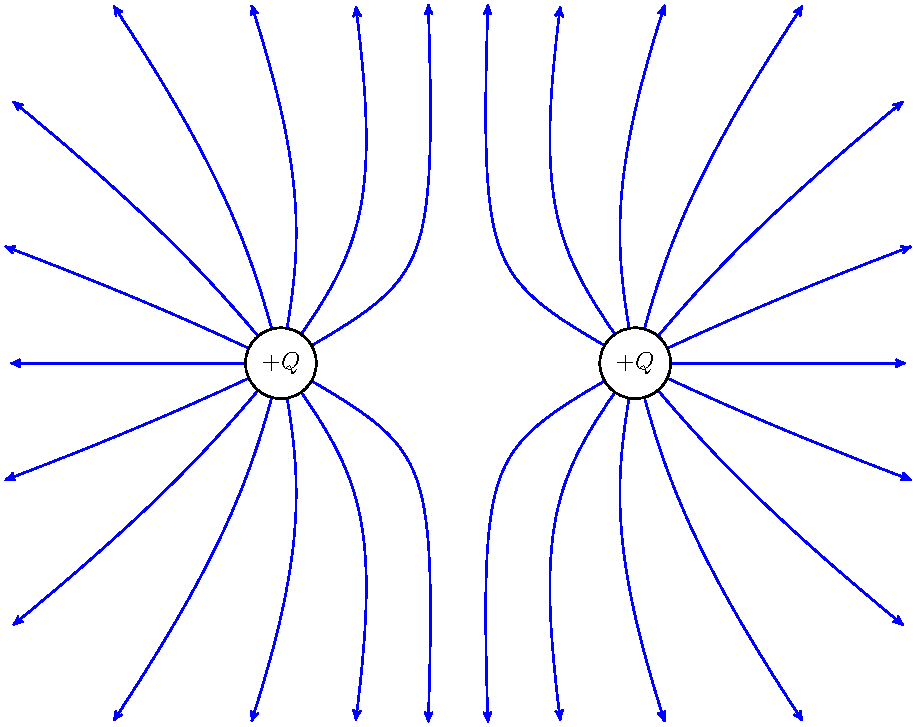
\includegraphics[width=7.2cm]{f-lines-eq-ch.pdf}
			\begin{equation*}
			\text{two positive charges}
			\end{equation*}
		\end{center}
	\end{minipage}\hfill
	\begin{minipage}{0.48\textwidth}
		\begin{center}
			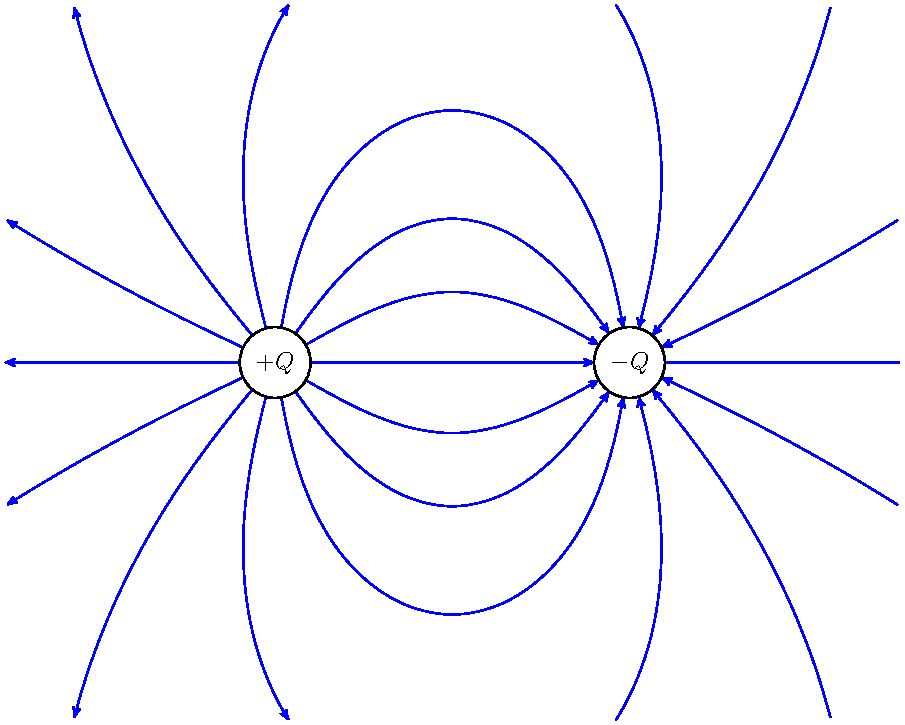
\includegraphics[width=7.2cm]{f-lines-op-ch.pdf}
			\begin{equation*}
			\text{two opposite charges} 
			\end{equation*}
		\end{center}	
	\end{minipage}
\end{figure*}

\section{Potential \& potential energy }

\subsection{Electric potential energy}
\label{sec:electric-potential}

The gain/loss in \keypoint{electric potential energy}\index{electric field!electric potential energy} is defined as work done against/by electric force, (compare everything in this chapter with what you have learned about gravitational P.E.!). Let's start to derive the electrical P.E. between two charges $Q$ and $q$ separated by $r$. Again we define $E_p=0$ at $r=\infty$ (choice of zero potential energy, no force so no P.E.), then:

\begin{ilight}
	\keypoint{Electric potential energy} is equal to the work done by electric force to bring a charge to a specific position from \emph{infinity}
\end{ilight} 

Moving a test charge $q$ from $r=\infty$ to a distance of $r$ from $Q$

\begin{center}
\begin{tikzpicture}[scale=0.8]
\draw [fill] (-4,0) circle [radius=0.1];
\node[below] at (-4,-0.1) {$Q$};
\draw [fill] (8,0) circle [radius=0.1];
\node[below] at (8,-0.1) {$q$};
\draw [thick, <->] (0,-1.2) --(-4,-1.2) node[above,midway]{$r$};
\draw [thick,dashed,gray,->] (7.7,0) -- (0.3,0) node[above,midway]{\textcolor{black}{$W$}};
\draw [fill] (0,0) circle [radius=0.1];
\draw (8,-1) node{$\infty$};
\end{tikzpicture}
\end{center}

work done by electric force: $$W=\int^r_\infty F dr = \int^r_\infty \frac{Qq}{\ec} \frac{\dd x}{x^2} = - \frac{Qq}{\ec x}\bigg|^r_\infty = - \frac{Qq}{\ec r} $$

Since: $\Delta E_p=-W$, we find: $$E_p(r) - E_p(_\infty) = \frac{Qq}{\ec r}$$

but $E_p(_\infty) = 0$,  so electric P.E. between two charges $Q$ and $q$ is $$\tcbhighmath{E_p(r) = \frac{Qq}{\ec r}}$$

As $r \to \infty$, $E_p \to 0$, this agrees with our definition for zero P.E. point. For like charges, $Qq > 0$, so $E_p > 0$, to bring like charges closer, work must be done to overcome their \emph{repulsion}, and P.E. increases.

The minimum P.E. $E_p(\infty)=0$ is at infinity, so positive P.E. at finite $r$. 

For opposite charges, $Qq < 0$, so $E_p < 0$, to pull opposite charges apart, work must be done to overcome their \emph{attraction}, P.E. increases.

The maximum P.E. $E_p(\infty)=0$ at infinity, so negative P.E. at finite $r$.

Note that electric P.E. is a \emph{scalar quantity}, sign is important however as repulsion implies positive P.E., and attraction implies negative P.E. Sometimes the sign of P.E. is hidden by the polarities of charges.

	

\subsection{Electric potential}

It is also useful to define the \emph{electric potential} for any specific point in a field. The electric potential can be thought as the electric potential energy per unit charge: $V = \frac{E_p}{q}$

\begin{ilight}
	\keypoint{Electric potential}\index{electric field!electric potential} is the work needed to bring a unit positive charge from infinity
\end{ilight}

\cmt unit: $[V] = \text{ J C}^{-1} = \text{V}$

\cmt electric potential due to an isolated source $Q$: $V = \frac{E_p}{q} = \frac{\frac{Qq}{\ec r}}{q} \RA$ $$\tcbhighmath{V = \frac{Q}{4\pi\epsilon_0 r}}$$

Potential at infinity vanishes: $V_\infty = 0$

Electric potential can take both signs, the sign depends on whether unit positive charge is repelled or attracted by the source. For positively-charged sources $V>0$, while for negatively-charged sources $V<0$. 

\cmt electric potential is a \emph{scalar} quantity so to find combined potential due to multiple charges, simply add up contributions of each charge.

\begin{figure}[ht]
	\centering
	\begin{tikzpicture}
		\draw[thick] (-5,0) circle(0.8) node[above]{$A$} (5,0) circle(0.8) node[above]{$B$};
		\draw[thick,dashed] (-5,-2.1) -- (-5,0) -- (5,0) -- (5,-2.1) (-2,0) node[above]{$P$} -- (-2,-1.5)
		(0,0) node[above]{$M$} -- (0,-1.5);
		\draw[fill] (-2,0) circle(0.05);
		\draw[fill] (0,0) circle(0.05);
		\draw[<->] (-5,-2.0) -- (5,-2.0) node[midway,above]{$10$ cm};
		\draw[<->] (-5,-1.2) -- (-2,-1.2) node[midway,above]{$3.0$ cm};
		\draw[<->] (0,-1.2) -- (-2,-1.2) node[midway,above]{$2.0$ cm};
	\end{tikzpicture}
\end{figure}

(a) Find the electric potential at point $P$ and point $M$ respectively.

(b) Find the work done to move an $\alpha$-particle from $P$ to $M$.

\label{ex-V-of-two-pcs}

\begin{figure}[ht]
	\centering
	\begin{tikzpicture}[scale=1.2]
		\draw[style=help lines,step=0.2,gray!50] (0,-0) grid (6,5);
		\draw[step=1] (0,0) grid (6,5);
		\draw [very thick, color=blue, domain=0.5:5.5, smooth, samples=60, variable=\x] plot (\x,{2.2/\x + 1.1/(6-\x)});
		\draw[very thick,blue] (0,4.6) --++ (0.5,0) node[above]{$A$};
		\draw[very thick,blue] (5.5,2.6) node[above]{$B$} --++ (0.5,0);
		\foreach \x in {0,100,200,300,400,500} \node[left] at (0,\x/100) {$\x$};
		\foreach \x in {0,2,4,6,8,10,12} \node[below] at (\x/2,0) {$\x$};
		\node at (-1.35,2.5) {$V/\text{V}$};
		\node at (3,-0.8) {$x/\text{cm}$};
	\end{tikzpicture}
\end{figure}

\rcyskip (a) Find the maximum speed as the proton moves from $A$ to $B$.

(b) Find the speed when the proton reaches surface of $B$.

\subsection{Equipotential lines}

To show potential distributions, we draw \keypoint{equipotential lines}\index{equipotential lines}
\footnote{In three dimensions, these lines form equipotential \emph{surfaces}.}. Points on same equipotential line have constant electric potential, i.e., equipotential lines are \emph{contour lines} of equal electric potential. For a field near a point charge, equipotential lines are a set of \emph{concentric} circles

\begin{center}
	\begin{tikzpicture}[scale=1.35]
	\draw (-2.7,0) node{$+Q$} circle [radius=0.5];
	\foreach \s in {0,45,90,...,315}
	\draw [blue, thick, ->] (-2.7,0) ++ (\s:0.5) -- ++(\s:1.8);
	
	\draw (2.7,0) node{$-Q$} circle [radius=0.5];
	\foreach \s in {0,45,90,...,315}
	\draw [blue, thick, <-] (2.7,0) ++ (\s:0.5) -- ++(\s:1.8);
	
	\foreach \s in {0.9,1.4,1.9}{
		\draw [red,dashed] (-2.7,0) circle(\s) (2.7,0) circle(\s);}
	\end{tikzpicture}
\end{center}

\cmt For uniform fields, equipotential lines are a set of \emph{parallel} straight lines

\begin{center}
	\begin{tikzpicture}[yscale=1.2]
	\draw (-5,1.2) rectangle (5,1.6);
	\draw (-5,-1.2) rectangle (5,-1.6);
	\foreach \charge in {-4.5,-3.5,...,4.5}{
		\draw (\charge,1.4) node {$+$} (\charge,-1.4) node {$-$};
		\draw[thick,blue,->] (\charge,1.2) --++ (0,-2.4);	
	}
	\foreach \s in {-0.8,0,0.8} \draw[red,dashed] (-5,\s) -- (5,\s);
	\end{tikzpicture}
\end{center}
	

	
Equipotential lines are always perpendicular to the electric field lines and moving along an equipotential line requires no work done.

\begin{figure*}
	\noindent\begin{minipage}{0.48\textwidth}
		\begin{center}
			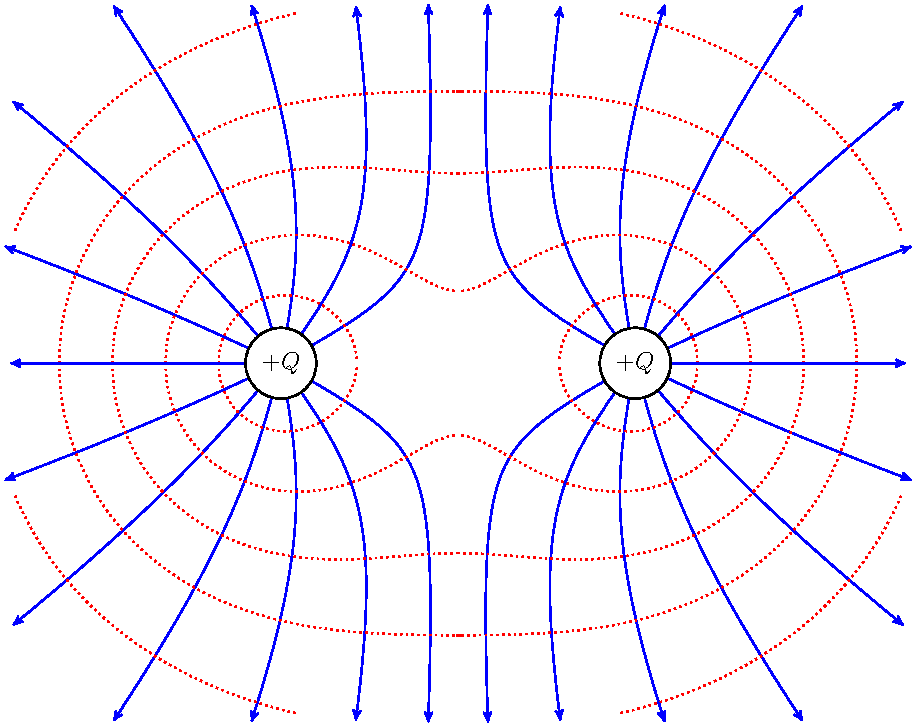
\includegraphics[width=7cm]{f-all-eq-ch.pdf}
		\end{center}
	\end{minipage}\hfill
	\begin{minipage}{0.48\textwidth}
		\begin{center}
			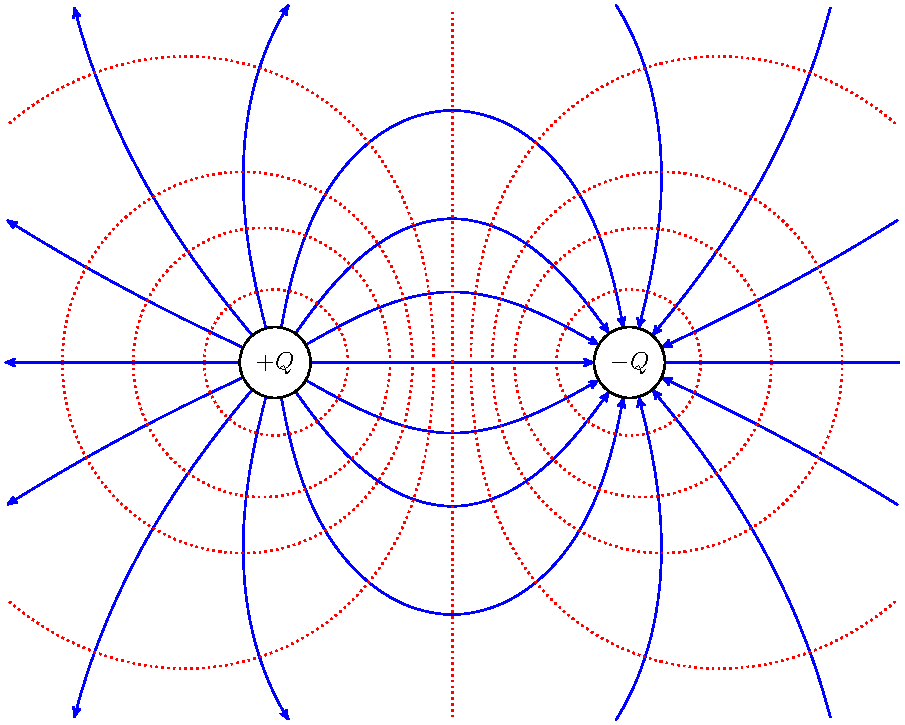
\includegraphics[width=7cm]{f-all-op-ch.pdf}
		\end{center}
	\end{minipage}
\end{figure*}

\begin{figure*}	
	\noindent\begin{minipage}{0.48\textwidth}
		\begin{center}	
			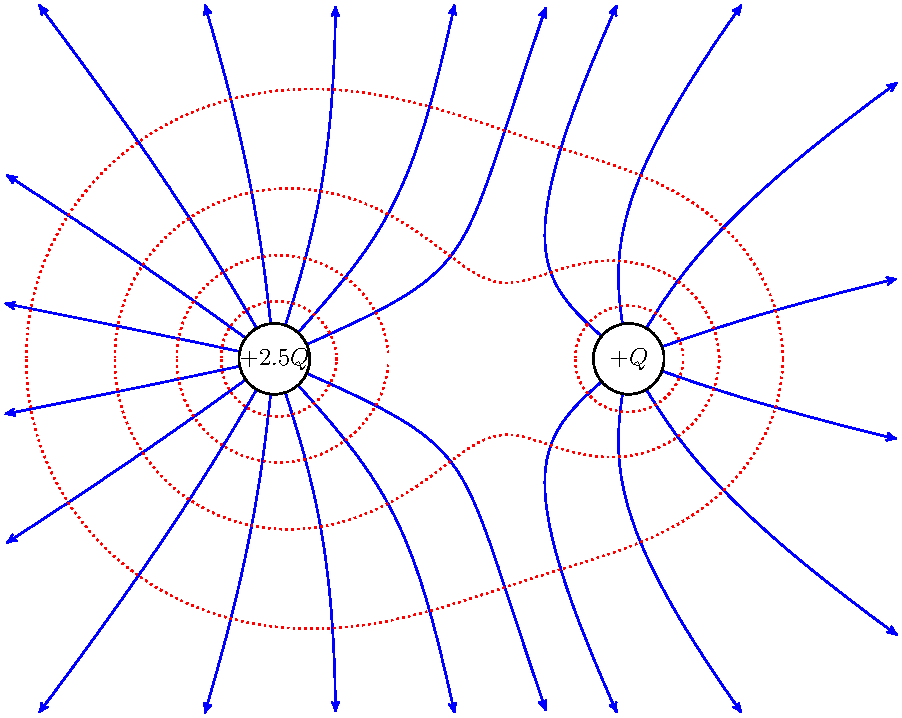
\includegraphics[width=7cm]{Q2p.pdf}
			\end{center}
		\end{minipage}\hfill
	\begin{minipage}{0.48\textwidth}
		\begin{center}
			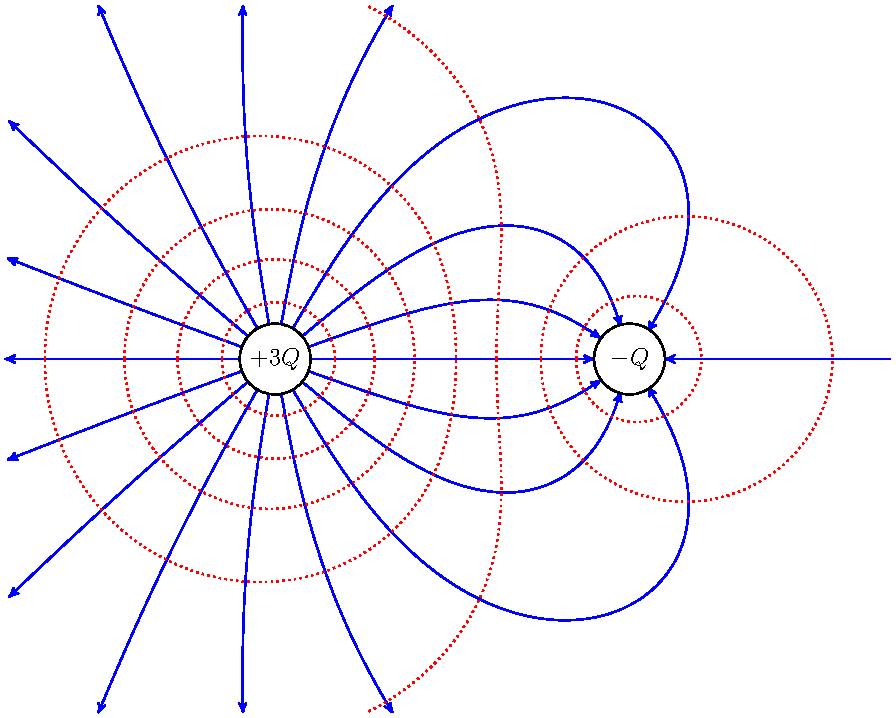
\includegraphics[width=7cm]{Q4n.pdf}
		\end{center}
	\end{minipage}
\end{figure*}

\begin{figure*}	
	\noindent\begin{minipage}{0.48\textwidth}	
		\begin{center}	
			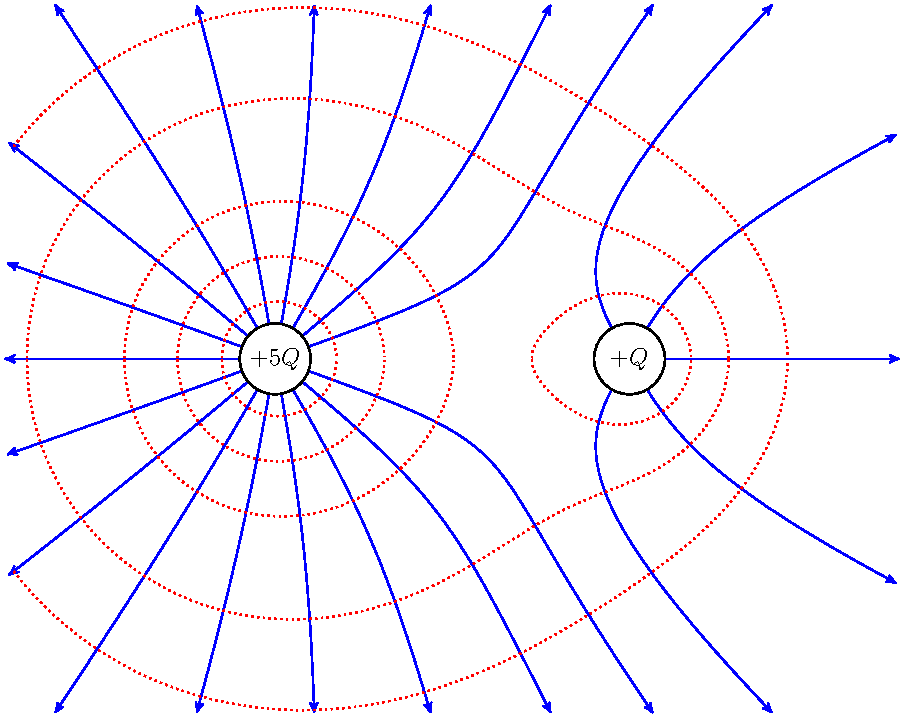
\includegraphics[width=7cm]{Q5p.pdf}
		\end{center}
	\end{minipage}\hfill
	\begin{minipage}{0.48\textwidth}
		\begin{center}
			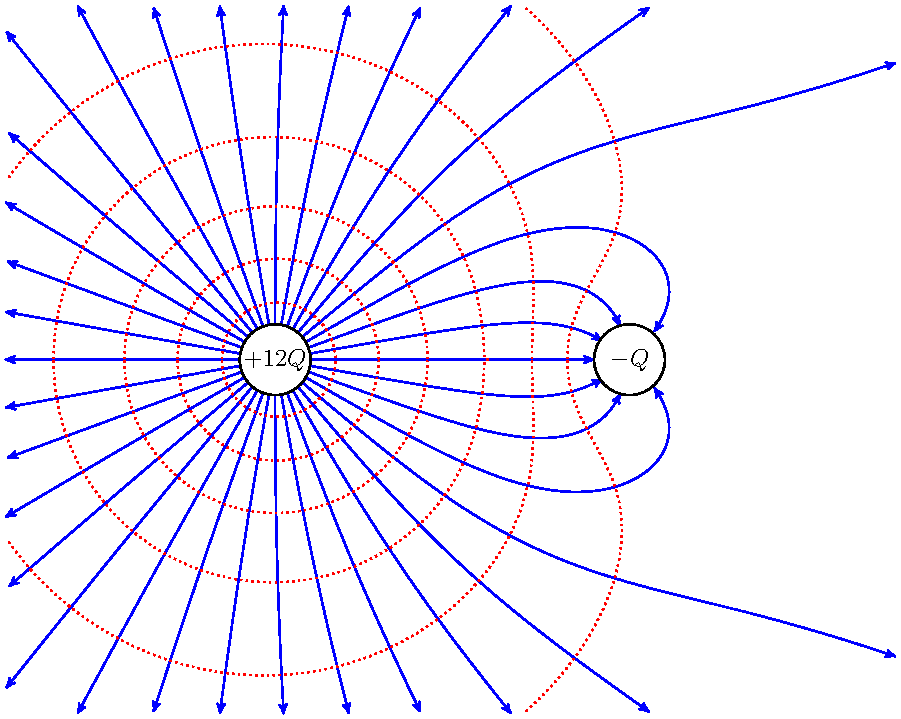
\includegraphics[width=7cm]{Q12n.pdf}
		\end{center}	
	\end{minipage}
\end{figure*}

\subsection{Further discussions on electric fields}

\subsection{A comparison with gravitational fields}

Both gravitational and electric force are described by inverse square law, so it follows that the mathematical language for both theories are very similar\footnote{Note that there is no negative mass, gravitational force always interacts attractively. This is the fundamental difference between gravitational fields and electric fields.}.

\begin{center}
	\begin{tabular}{|c|c|c|}
		\hline
		& vector description & scalar description \\ \hline 
		interaction between two masses/charges & force $F$ & potential energy $E_p$ \\ \hline
		effect of source mass/charge & field $g$/$E$ & potential $\varphi$/$V$ \\ \hline
	\end{tabular}
\end{center}

\begin{center}
{\renewcommand{\arraystretch}{1.28}
\begin{tabular}{|c|c|c|c|}
\hline
& gravitational field & electric field & meaning \\ \hline 
force & $F=(-)G \frac{Mm}{r^2}$ & $F=\frac{1}{4\pi\epsilon_0} \frac{Qq}{r^2}$ & force between masses/charges\\ [1ex] \hline
field strength & $g= \frac{F}{m} = (-)G \frac{M}{r^2}$ & $E= \frac{F}{q} = \frac{1}{4\pi\epsilon_0} \frac{Q}{r^2}$ & force per unit mass/charge\\ [1ex] \hline
potential energy &  $E_p = -G \frac{Mm}{r}$ & $E_p=\frac{1}{4\pi\epsilon_0} \frac{Qq}{r}$ & related to work done by force \\ [1ex] \hline
potential & $\varphi = \frac{E_p}{m} = -G \frac{M}{r}$ & $V = \frac{E_p}{q} = \frac{1}{4\pi\epsilon_0} \frac{Q}{r}$ & energy per unit mass/charge\\ [1ex] \hline
\end{tabular}}
\end{center}

Similarities between gravitational field and electric field:

\begin{itemize}
	\item[-] force and field strength both obey \emph{inverse square laws}
	
	\item[-] potential energy and potential is inversely proportional to separation
	
	\item[-] no potential energy and no potential at infinite separation
\end{itemize}

Differences between gravitational field and electric field:

\begin{itemize}

\item[-] Mass (source of gravity) is always positive, but electric charges can be positive or negative - this fact leads to many fundamental differences between the two force fields
\item[-] electric force can be repulsive or attractive, but gravitational force is always attractive

\item[-] electric potential can take both signs, but gravitational potential is always negative
\end{itemize}

\subsection{Electric field inside conductors}\label{inside-conductors}

Consider electric field \emph{inside} a metal conductor carrying charge $Q$. the fact that the shell is a conductor means there are free charge carriers that can move around but charge distribution should be stable for a charged conductor (no circulating currents) so charge carriers must experience no force, i.e., field strength inside conductor is zero. To put it the other way round, if there is an excess field, it will push free charge carriers to move around, until they are distributed so that the field inside the conductor becomes zero. Moreover, there shall be no potential difference between any two points inside the conductor, otherwise charge carriers would flow, so electric potential must be constant.

\begin{ilight}
	\centering
	
	Electric field strength is everywhere zero inside a conductor: $E=0$
	
	Electric potential is everywhere constant inside a conductor: $V=\text{const}$
\end{ilight}

\label{ex-metal-sphere}

\begin{figure*}[ht]
	\centering
	\noindent\begin{minipage}{0.45\linewidth}
		\centering
		\begin{tikzpicture}[yscale=1.2,xscale=1.2]
		\draw[thick,<->] (0,5) node[left]{$E$} -- (0,0) -- (1,0) node[below]{$R$} -- (4.5,0) node[below]{$r$};
		\draw [thick,color=blue,domain=1:4.5,samples=20,smooth,variable=\x] plot (\x,{4.5/\x/\x});
		\draw[thick,blue] (0,0.02) -- (1,0.02);
		\draw[dashed] (0,4.5) node[left]{$E_0$} -- (1,4.5) -- (1,0) node[below]{$R$};
		\draw[dashed] (0,4.5/4) node[left]{{\scriptsize $\frac{E_0}{4}$}} -- (2,4.5/4) -- (2,0) node[below]{$2R$};
		\draw[dashed] (0,4.5/9) node[left]{{\scriptsize $\frac{E_0}{9}$}} -- (3,4.5/9) -- (3,0) node[below]{$3R$};
		\end{tikzpicture}
		

	\end{minipage}
	\begin{minipage}{0.45\linewidth}
		\centering
		\begin{tikzpicture}[yscale=1.2,xscale=1.2]
		\draw[thick,<->] (0,5) node[left]{$V$} -- (0,0) -- (1,0) node[below]{$R$} -- (4.5,0) node[below]{$r$};
		\draw [thick,color=blue,domain=1:4.5,samples=20,smooth,variable=\x] plot (\x,{4.5/\x});
		\draw[dashed] (0,4.5) node[left]{$V_0$} -- (1,4.5) -- (1,0) node[below]{$R$};
		\draw[dashed] (0,4.5/2) node[left]{{\scriptsize $\frac{V_0}{2}$}} -- (2,4.5/2) -- (2,0) node[below]{$2R$};
		\draw[dashed] (0,4.5/3) node[left]{{\scriptsize $\frac{V_0}{3}$}} -- (3,4.5/3) -- (3,0) node[below]{$3R$};
		\draw[thick,blue] (0,4.5) -- (1,4.5);
		\end{tikzpicture}
		

	\end{minipage}

\caption{Example \ref{ex-metal-sphere}: field strength and potential due to a charged metal sphere}
\end{figure*}

\subsection{Field strength \& potential}\label{field-strength-potential}

For a small displacement $\Delta r$ in an electric field, change in potential $\Delta V$ is

{

\centering

$\Delta V = \frac{\Delta E_p}{q} \xlongequal{\Delta E_p=-W} - \frac{\Delta W}{q} = - \frac{F \Delta r}{q} \xlongequal{F=Eq} - E \Delta r \RA E = - \frac{\Delta V}{\Delta r}$

}

\eqyskip as change in displacement $\Delta r \to 0$, we have $$\tcbhighmath{E = - \frac{\dd V}{\dd r}}$$

therefore we have the following theorem:

\begin{ilight}
	\centering Field strength is negative gradient of potential with respect to displacement.
\end{ilight}

One can also consider change in potential $\Delta V$ for large distance due to work done in a field

{
	
\centering

$\Delta V= \int \dd V \xlongequal{E = -\dd V/\dd r}  \int (-)E \dd r =  -\int E \dd r$
\footnote{The expression is implicitly integrated from initial position to final position.}

}

\eqyskip this gives the inverse relation: $$\tcbhighmath{\Delta V = -\int E \dd r}$$
\footnote{These equations are correct if the charge is moving in the parallel direction to the field, i.e., the motion is along the field lines. But an object can move in all directions in the field. More rigorously, if we take the vector nature of electric field into account, we should write $\Delta V = - \int \mathbf{E}\cdot\dd\mathbf{r}$, and $\mathbf{E} = - \frac{\partial V}{\partial \mathbf{r}}$. \piste}

\cmt given a $V$-$r$ graph, gradient of curve gives field strength

conversely, given a $E$-$r$ graph, area under curve gives change in potential

\cmt can also write $F = - \frac{\dd U}{\dd r}$ and $\Delta U = -\int F \dd r$

force always acts in a direction to lower the potential energy of an object
\footnote{This result can be generalised to a very important principle of physical laws called the \emph{least action principle}. It states that any motion of a system tends to minimise the action, a physical quantity related to the energy of the system. This fundamental law plays a crucial role in the study of theoretical physics. \piste}

\label{ex-grad-pot}

\begin{figure}[ht]
	\centering
	\begin{tikzpicture}[scale=0.54]
	\draw[style=help lines,step=0.5,gray!30] (0,0) grid (12,12);
	\draw[style=help lines,step=2] (0,0) grid (12,12);
	\draw [thick] (12,0) node[below]{$r/\text{cm}$};
	\draw [thick] (0,12) node[left]{$V/\text{kV}$};
	\foreach \s in {0,2,...,10}
	{
		\draw (\s,0) node[below]{\s};
		\draw (0,\s) node[left]{\s};
	}
	\draw[very thick,purple,domain=2:10,samples=15,smooth,variable=\x] plot (\x,20/\x);
	\draw[thick,red,domain=1:9,samples=2,smooth,variable=\x] plot (\x,-0.8*\x+8);
	\draw[fill] (5,4) circle[radius=0.15];
	\draw[thick,blue] (2,6.5) -- (2,1.5) -- (8,1.5);
	\end{tikzpicture}
\end{figure}

 

\newpage

\begin{figure}[ht]
	\centering
	\begin{tikzpicture}[scale=1.35]
	\draw[style=help lines,step=0.25,gray!30] (0,-2) grid (8,4);
	\draw[style=help lines,step=1] (0,-2) grid (8,4);
	\node[left] at (0,4) {$V$};
	\node[left] at (0,0) {0};
	\foreach \x in {0,1,...,8} {
		\draw[white,fill] (\x-0.1,-0.32) rectangle (\x+0.1,-0.08);
		\node[below] at (\x,0) {$\x$};
	}
	\draw[thick, purple, domain=1:7, samples=25, smooth, variable=\x] plot (\x,{4/\x/\x-2/(8-\x)/(8-\x)});
	\node[right] at (8.1,0) {$x/\text{cm}$};
	\end{tikzpicture}
\end{figure}

\subsection*{Uniform fields revisited}

Given two oppositely-charged metal plates separated by a distance of $d$, if th p.d. between the plates is $V$, then electric field strength between is given by $E = \frac{V}{d}$. We will derive this result using the theorem introduced in the last chapter

\begin{figure}[ht]
\centering
\begin{minipage}{0.48\textwidth}
	\centering
	\begin{tikzpicture}[scale=0.8]
	\foreach \s in {1,2,3,4}
	\draw[thick,blue,<-] (0,\s) -- (5,\s);
	\draw (2.5,4) node[above]{$E$};
	\draw [thick,gray,dashed,<-] (1,2.5) -- (4,2.5);
	\shade [ball color = green] (4,2.5) circle [radius=0.1] node[right]{$q$};
	\draw [thick] (5,0.5) -- (5,4.5) node[above]{$+$};
	\draw [thick] (0,0.5) -- (0,4.5) node[above]{$-$};
	\draw[<->] (0,0) -- (5,0) node[midway, above] {$d$};
	\end{tikzpicture}
\end{minipage}\hfil
\begin{minipage}{0.48\textwidth}
	\centering
	\begin{tikzpicture}[scale=0.8]
		\draw [thick,<->] (0,4.2) node[left]{$V$} -- (0,0) -- (5.6,0) node[below]{$r$};
		\draw[dashed] (5,3.6) -- (5,0) node[below]{$d$}; 
		\draw [very thick,red] (0,0) -- (5,3.6);
	\end{tikzpicture}
\end{minipage}
\captionsetup{labelformat=empty}

\caption{moving a test charge in a uniform electric field}
\end{figure}

Moving a test charge $q$ in a uniform field, work done by electric force: $W=Fd = Eqd$
		
Change in P.E.: $\Delta E_p = -W = -Eqd$

Change in potential: $\Delta V = \frac{\Delta E_p}{q} = - Ed$, or $E=-\frac{\Delta V}{d}$

Potting $V$-$r$ graph, $\text{gradient of line}=-E$.

The minus sign means field strength points in the direction such that potential decreases.

i.e., electric field acts from high potential to low potential.

\subsection*{The electric field due to two positive point charges}

Two point charges $+Q_1$, $+Q_2$ are separated by a distance of $D$, let's look into the electric field along the segment joining the two charges:

\begin{center}
\begin{tikzpicture}[scale=0.8]
\shade [ball color = green] (-4,0) node[above]{$+Q_1$} circle (0.15);
\shade [ball color = green] (4,0) node[above]{$+Q_2$} circle (0.15);
\draw [thick, <->] (-4,-2)--(4,-2) node[midway,above]{$D$} ;
\draw [thick, <->] (-4,-1)--(-1,-1) node[midway,above]{$r_1=x$};
\draw [thick, <->] (-1,-1)--(4,-1) node[midway,above]{$r_2=D-x$};
\draw [thick, <->] (-4,-2)--(4,-2) node[midway,above]{$D$} ;
\draw [dashed] (-4,-0.5) -- (-4,-2.2);
\draw [dashed] (4,-0.5) -- (4,-2.2);
\draw [dashed] (-1,-0.5) -- (-1,-1.5);
\draw [->,thick,blue] (-1,0) -- ++(-0.9,0) node[above]{$E_2$};
\draw [->,thick,blue] (-1,0) -- ++(2.5,0) node[above]{$E_1$};
\draw [fill] (-1,0) node[above]{$q$} circle [radius=0.1];
\end{tikzpicture}
\end{center}

The combined potential: $V = V_1 + V_2 = \frac{Q_1}{4\pi\epsilon_0r_1} + \frac{Q_2}{4\pi\epsilon_0r_2} = \frac{1}{4\pi\epsilon_0}\left(\frac{Q_1}{x} + \frac{Q_2}{D-x}\right)$

The combined field strength: $E = E_1 - E_2 = \frac{Q_1}{4\pi\epsilon_0r_1^2} - \frac{Q_2}{4\pi\epsilon_0r_2^2} = \frac{1}{4\pi\epsilon_0}\left(\frac{Q_1}{x^2} - \frac{Q_2}{(D-x)^2}\right)$

Notice that when computing $V$, we carry out \emph{scalar sum} but for $E$, we carry out a \emph{vector sum}, i.e., directions of $E_1$ and $E_2$ become important.

\begin{figure*}
\begin{center}
	\begin{tikzpicture}[scale=1.35]
	\draw[thick,->] (0,-2) -- (0,4.8);
	\draw[thick,->] (0,0) -- (9,0) node[below]{$x$};
	\draw [thick,color=blue,domain=0.3:7.7,samples=60,smooth,variable=\x] plot (\x,{(.24/\x/\x-.08/(8-\x)/(8-\x))*1.5}) node[below]{$E$};
	\draw [thick,color=red,domain=0.3:7.7,samples=60,smooth,variable=\x] plot (\x,{(.3*3/\x+.1*3/(8-\x))*1.5}) node[above]{$V$};
	\draw[dashed] (8,-2) -- (8,3);
	\shade [ball color = green] (0,0) node[below right]{$+Q_1$} circle (0.15);
	\shade [ball color = green] (8,0) node[below right]{$+Q_2$} circle (0.15);
	\end{tikzpicture}
\end{center}
\caption{$V$-$x$ graph and $E$-$x$ graph for the case where $Q_1=3Q_2$ are sketched.}
\end{figure*}

\cleardoublepage

% ===== Chapter: 24-capacitance =====
\chapter{Capacitors}

\section{Capacitors: an introduction}

\begin{marginfigure}
\begin{tikzpicture}[scale=0.5]
\coordinate (A1) at (0,0); 
\coordinate (A2) at (0.5,0);
\coordinate (A3) at (2.5,0); 
\coordinate (A4) at (3,0);
\coordinate (B1) at (0,4); 
\coordinate (B2) at (0.5,4);
\coordinate (B3) at (2.5,4); 
\coordinate (B4) at (3,4);
\coordinate (C1) at (1.2,5.5); 
\coordinate (C2) at (1.7,5.5);
\coordinate (C3) at (3.7,5.5); 
\coordinate (C4) at (4.2,5.5);
\coordinate (D4) at (4.2,1.5);
\draw [thick,fill=gray!50] (A1) -- (A2) -- (B2) -- (C2) -- (C1) -- (B1) -- cycle;
\draw [thick,fill=cyan!20] (A2) -- (A3) -- (B3) -- (C3) -- (C2) -- (B2) -- cycle;
\draw [thick,fill=gray!50] (A3) -- (A4) -- (B4) -- (C4) -- (C3) -- (B3) -- cycle;
\draw [thick,fill=gray!50] (A4) -- (B4) -- (C4) -- (D4) -- cycle;
\draw [thick] (B1) -- (B4);
\draw [ultra thick] (3.6,2.7) [out=0, in=180] to (6,2) node[below]{lead};
\draw [ultra thick] (0,2.7) [out=180, in=0] to (-1.5,2) node[below]{lead};
\draw [thick] (3.6,4) -- ++ (1.5,1) node[right,align=center,execute at begin node=\setlength{\baselineskip}{1.2em}]{metal\\plate};
\draw [thick] (1.5,0.5) -- ++ (1.2,-1) node[right]{dielectric};
\end{tikzpicture}
\end{marginfigure}

\keypoint{Capacitors}\index{capacitor} are elementary electrical units widely used in electrical and electronic engineering. a typical capacitor has two conductive plates and between the plates there is usually an insulating material called \emph{dielectric}.

circuit symbol for a capacitor is:
\begin{figure}
    \centering
\begin{tikzpicture}[scale=0.2]
\draw (0,0) -- (1.6,0) (2.4,0) -- (4,0);
\draw (1.6,-1) -- (1.6,1) (2.4,-1) -- (2.4,1);
\end{tikzpicture}
\end{figure}
\vspace*{\baselineskip}

\begin{marginfigure}
\begin{circuitikz}[european resistors]
	\draw (2,-2) -- (-2,-2)  to[battery,l^=$\mathcal{E}$] (-2,2) -- (-0.5,2);
	\draw (2,-2) -- (2,-2)  to[R,l_=$R$] (2,2) -- (0.5,2);
	\draw (0,-2) -- (0,-1) to[C,l_=$C$] (0,1) -- (0,1.2);
	\draw[fill=white] (0.5,2) circle(0.06) node[above]{$Y$};
	\draw[fill=white] (-0.5,2) circle(0.06) node[above]{$X$};
	\draw[very thick] (0,1.2) --++ (80:1);
	\draw[fill=white] (0,1.2) circle(0.06) node[right]{$S$};
\end{circuitikz}
\end{marginfigure}

If we construct an electric circuit as shown, when contact $S$ is moved to $X$, capacitor is connected to a voltage supply and becomes charged. Positive and negative charges are separated onto two plates, and they will stay where they are even if we disconnect the capacitor from the voltage supply.

If we then move $S$ to $Y$, the charged capacitor discharges and drives a current through resistor $R$, i.e., it can act as a temporary power source\footnote{Details on charging and discharging processes will be gone through in \S\ref{sec:charging-capacitors}.}

So capacitors can be used to store and release energy, or more correctly, charge.\footnote{Other important functions of capacitors in electronic circuits include smoothing output voltage of power supplies, blocking direct current while allowing alternating current to pass, etc.}

\subsection{Capacitance}

To describe ability of a capacitor to store charges, we define the notion of capacitance

\begin{ilight}
	\keypoint{The capacitance}\index{capacitance!mutual capacitance} of a parallel-plate capacitor is defined as the ratio of the charge stored on each plate to the potential difference across the two plates.
\end{ilight}

In a word equation: $\text{Capacitance } C = \frac{\text{charge on one plate }Q }{\text{p.d. } V \text{ across the plates}} \quad \Rightarrow \quad$ $$\tcbhighmath{C = \frac{Q}{V}}$$

The unit of capacitance: \keypoint{farad}\index{farad}
\footnote{The unit is named after Michael Faraday, a British physicist who developed the concept of capacitance. Faraday's other main discoveries include electromagnetic induction and electrolysis. He established the basis for the concept of the electromagnetic field in physics.}
: $[C] = \text{F}$

It's a derived unit: $1 \text{ F} = 1 \text{ C}\cdot\text{V}^{-1}$

The Farad is a stupidly large unit for most applications, more common subunits of capacitance in use are sub-multiples of farad:

{
	
\centering

$1 \muF = 10^{-6} \text{ F}, \quad 1 \text{ nF} = 10^{-9} \text{ F}, \quad 1 \pF = 10^{-12} \text{ F}$

}

One important point that is often missed - for a parallel-plate capacitor, charges on the two plates are equal but opposite so the net charge on the capacitor: $Q_\text{net} = (+Q)+(-Q)=0$. 

I want to really emphasise that:
\begin{ilight}
    The charge in the definition is charge on \emph{one} plate \textbf{not} the difference between the plates.
\end{ilight}

The capacitance of a capacitor depends on \emph{geometry} of the device and permittivity of the dielectric material. It does not depend on electric field or potential\footnote{Recall the resistance of an electrical component. Resistance is defined as the ratio of p.d. to current, but the value of resistance is essentially dependent on the length, cross-sectional area and material of the component, instead of the p.d. applied or the current flowing through it.}

for example, capacitance between two metal plates isfootnote{If there is \emph{dielectric} in between, the formula should be rewritten as $C = \frac{\epsilon A}{d}$, where $\epsilon$ is permittivity of dielectric. These formulae are not examinable by the syllabus.}: $$\tcbhighmath{C=\frac{\epsilon_0 A}{d}}$$\

Where:\\
$A$ is area of plate, \\
$d$ is distance between plates, \\
both are geometrical quantities

% \subsection{self-capacitance}

% there are two closely related notions of capacitance: \emph{mutual} capacitance and \emph{self} capacitance

% the definition for capacitance given in the previous chapter, is actually \emph{mutual} capacitance\footnote{In many cases, the term capactiance is a shorthand for mutual capacitance.}

% on the other hand, all bodies are able to store electrical charge

% any object that can be electrically charged exhibits capacitance

% we define \keypoint{self-capacitance}\index{capacitance!self-capacitance} of an object as the amount of charge that must be added to increase per unit electrical potential

% in a word equation, $ \text{self capacitance }C=\frac{\text{charge of object }Q}{\text{electric potential of object }V} \RA \tcbhighmath{C=\frac{Q}{V}}$\footnote{For either mutual capacitance or self capacitance, defining equation $C=\frac{Q}{V}$ takes the same form, but you should keep in mind that $Q$ and $V$ represent different things in different contexts.}

% \example{Self-capacitance of a charged metal sphere in a vacuum}

% consider a metal sphere of radius $R$ and carries an electric charge of $Q$

% its electric potential: $V = \frac{Q}{\ec R}$

% \begin{soln}
% self-capacitance of the sphere: $C_\text{sphere} = \frac{Q}{V} = Q \times \frac{\ec R}{Q} \RA \tcbhighmath{C_\text{sphere} = \ec R}$

% note that capacitance is only dependent on its geometrical property (radius $R$) \end{soln}

% \example{A conducting sphere of radius 1.0 m is situated in free space. (a) Find its capacitance. (b) In order to raise its potential to 5000 V, find the amount of charge needed.}

% \begin{soln} capacitance of the sphere: $C = \ec R = 4\pi\times8.85\times10^{-12}\times 1.0 \approx 1.11\times10^{-10} \text{ F}$

% (here you can see farad being an impractically huge unit)

% charge on sphere: $Q = CV = 1.11\times10^{-10} \times 5000 \approx 5.56\times 10^{-7} \text{ C}$ \end{soln}

\subsection*{Analogy with ideal gases}

an interesting analogy can be made between capacitors and ideal gases

recall an ideal gas is described by equation $pV=nRT$
\footnote{Don't confuse voltage $V$ with volume $V$!}

compare $\left\{\begin{array}{lccl}
\text{amount of charge:} & Q & = &CV \\ \text{amount of substance:} &n & = & \left(\frac{V}{RT}\right) p
\end{array}\right.$

\eqyskip
volume $V$ of a container has a certain space \emph{capacity}, at fixed $T$, pumping more gas (increase $n$) into system, pressure $p$ increases

similarly, a capacitor has a certain charge capacity, adding more charge $Q$ increases p.d. $V$, so the quantity $C$ is naturally called \emph{capacitance}

also for a container, there exists a maximum pressure which it can withstand

for a capacitor, there exists a \emph{breakdown voltage}, or \emph{withstand voltage}, beyond which there could be sparkling across the capacitor

\subsection{Energy stored in a capacitor}

To charge a capacitor, we need to push electrons off one plate and onto the other, the separation of positive and negative charges requires work done $\ra$ energy is stored.

\begin{marginfigure}
	\vspace*{-8pt}
	\centering
	\begin{tikzpicture}[scale=1]
	\draw [gray!50, fill] (0,0) -- (3.5,2.5) -- (3.5,0) -- cycle;
	\draw [thick,<->] (0,3) node[left]{$V$} -- (0,0) -- (4,0) node[below]{$Q$};
	\draw [ultra thick, blue] (0,0) -- (3.5,2.5);
	\draw (2.5,1) -- (1.6,2) node[above,align=center,execute at begin node=\setlength{\baselineskip}{1.2em}]{energy\\stored};
	\end{tikzpicture}
	\vspace*{-16pt}
\end{marginfigure}

Since charge $Q$ varies with p.d. $V$, we shall use the $V$-$Q$ graph to find work done $W$, the area under $V$-$Q$ graph is equal to work done $W$

{
	
	\centering
	
	$W = \frac{1}{2} QV$
	
}

Substituting $Q=CV$, the energy stored in capacitor is\footnote{Rigorously speaking, this electrical potential energy is stored within the \emph{electric fields} between metal plates of capacitor.}:

{

\centering

$\tcbhighmath{W = \frac{1}{2}CV^2 = \frac{Q^2}{2C}}$

} 

\newpage

\subsection{Capacitor networks}

\subsection{Capacitors in parallel}

\begin{marginfigure}
\vspace*{-20pt}
\centering
\begin{circuitikz}[european resistors,scale=0.9]
\draw (0,0) -- (0,1.6) to[C] (3,1.6) -- (3,0) to[C] (0,0);
\node [below] at (2.1,1.6) {$C_1$};
\node [below] at (0.9,1.6) {$Q_1$};
\node [below] at (2.1,0) {$C_2$};
\node [below] at (0.9,0) {$Q_2$};
\draw (-1,0.8) -- (0,0.8) (3,0.8) -- (4,0.8);
\draw [<->] (0,2.5) -- (1.5,2.5)node[above]{$V$} -- (3,2.5);
\foreach \y  in {0,3} \draw (\y,2.3) -- (\y,2.7);
\end{circuitikz}
\end{marginfigure}

Consider two capacitors connected in parallel, they have the same p.d. $V$ across the network: $V=V_1=V_2$, but charge $Q$ is shared: $$Q_\text{total} = Q_1 + Q_2$$

{

\centering

$\frac{Q_\text{total}}{V} = \frac{Q_1}{V} + \frac{Q_2}{V}$

$C_\text{total} = C_1 + C_2$

}

If three of more capacitors in parallel: $$\tcbhighmath{C_\text{total} = C_1 + C_2 + C_3 + \cdots}$$ and... $$\tcbhighmath{Q_\text{total} = Q_1 + Q_2 + Q_3 + \cdots}$$

Adding an extra capacitor in parallel to a network, will cause the total capacitance to increase.

In terms of the physical structure of the plates - when several capacitors connected in parallel, equivalent to a single capacitor with larger plates, so more charge on the plates $\ra$ $C\up$.

\newpage

\subsection{Capacitors in series}

\begin{marginfigure}

\centering
\begin{circuitikz}[european resistors,xscale=0.7]
\draw (0,0) to[C, l_=$C_1$] (4,0) to[C, l_=$C_2$] (8,0);
\node [below] at (2.9,0) {$-Q$};
\node [below] at (1.1,0) {$+Q$};
\node [below] at (6.9,0) {$-Q$};
\node [below] at (5.1,0) {$+Q$};
\draw [<->] (0,1) -- (2,1)node[above]{$V_1$} -- (4,1);
\draw [<->] (4,1) -- (6,1)node[above]{$V_2$} -- (8,1);
\foreach \y  in {0,4,8} \draw (\y,0.8) -- (\y,1.2);
\draw [<->] (0,2) -- (4,2)node[above]{$V$} -- (8,2);
\foreach \y  in {0,8} \draw (\y,1.8) -- (\y,2.2);
\end{circuitikz}

\end{marginfigure}

Consider two series capacitors, with the same charge $Q$ on each plate: $$Q=Q_1=Q_2$$\footnote{Initially, the H-shaped isolated section between capacitors is uncharged. But no charge can enter or leave this section, its net charge must remain zero. Since a capacitor carries equal and opposite charges on its plates, so every capacitor in series carries same charge $Q$}

The p.d. is shared: $V_\text{total} = V_1 + V_2$ so..

{
	
	\centering
	
	$\frac{V_\text{total}}{Q} = \frac{V_1}{Q} + \frac{V_2}{Q}$
	
	\eqyskip
	
	$\frac{1}{C_\text{total}} = \frac{1}{C_1} + \frac{1}{C_2} $
	
}

if three of more capacitors in series: 
$$\tcbhighmath{\frac{1}{C_\text{total}} = \frac{1}{C_1} + \frac{1}{C_2} + \frac{1}{C_3} + \cdots}$$ and... $$\tcbhighmath{V_\text{total} = V_1 + V_2 + V_3 + \cdots}$$

Adding an extra capacitor in series to a network will cause the total capacitance to decrease. 
In physical terms, when several capacitors connected in series, equivalent to a parallel-plate capacitor with greater separation, so more charge on the plates $\ra$ $C\down$.

\begin{figure}
	\begin{circuitikz}[european resistors,scale=0.9]
		\draw (0,0) to[C,l_=$C_1{=}4.0\mu\text{F}$] (3,0) to[C,l_=$C_2{=}12\mu\text{F}$] (6,0) -- (6,3) to[battery,l_=$V{=}8.0\text{V}$] (0,3) -- (0,0);
	\end{circuitikz}
\end{figure}

\subsection{Capacitor networks}

More complicated capacitor networks can be considered as a combination of some smaller networks with capacitors in parallel or in series.

\label{ex-Cnet}

{
	
	\centering
	
	\begin{circuitikz}[european resistors,scale=0.75]
		\draw (0,0) -- (0,2) to[C,l^=$C$] (3,2) -- (3,0) to[C,l^=$C$] (0,0);
		\draw (-3,1) to[C,l^=$C$] (0,1);
		\draw (3,1) to[C,l^=$C$] (6,1);
	\end{circuitikz}

}

 

\subsection{Capacitors \& resistors}

As a quick review, we compare capacitor networks with resistor networks.
\begin{fullwidth}
{\renewcommand{\arraystretch}{2}
\begin{tabular}{|c|c|c|}
\hline
& capacitors & resistors \\ \hline
\multirow{4}{*}{in series}  & same charge & same current \\ [-1ex]
& \multirow{2}{*}{\begin{circuitikz}[european resistors,scale=0.75]
\draw (-0.3,0) -- (0,0) to[C, l^=$C_1$] (2,0) to[C, l^=$C_2$] (4,0) to[C, l^=$C_3$] (6,0) -- (6.3,0) node[right]{$\cdots$};
\end{circuitikz}}  & \multirow{2}{*}{\begin{circuitikz}[european resistors,scale=0.75]
\draw (-0.3,0) -- (0,0) to[R, l^=$R_1$] (2,0) to[R, l^=$R_2$] (4,0) to[R, l^=$R_3$] (6,0) -- (6.3,0) node[right]{$\cdots$};
\end{circuitikz}}  \\
 & & \\ [-1ex]
 & $\frac{1}{C_\text{total}} = \frac{1}{C_1} + \frac{1}{C_2} + \frac{1}{C_3} + \cdots$ & $R_\text{total} = R_1 + R_2 + R_3 + \cdots$ \\ [1.5ex] \hline
\multirow{6}{*}{in parallel}  & same p.d. across & same p.d. across \\ [0ex]
& \multirow{4}{*}{\begin{circuitikz}[european resistors,scale=0.6]
\foreach \x  in {1,2,3} {
\draw (0,6-2*\x) to[C] (4,6-2*\x);
\node[above] at (1.25,6.3-2*\x) {$C_\x$};
}
\draw (-1.5,2) -- (0,2) (4,2) -- (5.5,2);
\draw (0,4) -- (0,0) node[below]{$\vdots$} (4,4) -- (4,0) node[below]{$\vdots$};
\end{circuitikz}}  & \multirow{4}{*}{\begin{circuitikz}[european resistors,scale=0.6]
\foreach \x  in {1,2,3} {
\draw (0,6-2*\x) to[R,l^=$R_\x$] (4,6-2*\x);
}
\draw (-1.5,2) -- (0,2) (4,2) -- (5.5,2);
\draw (0,4) -- (0,0) node[below]{$\vdots$} (4,4) -- (4,0) node[below]{$\vdots$};
\end{circuitikz}}  \\
 & & \\
 & & \\
 & & \\ [0.4ex]
 & $C_\text{total} = C_1 + C_2 + C_3 + \cdots$ & $\frac{1}{R_\text{total}} = \frac{1}{R_1} + \frac{1}{R_2} + \frac{1}{R_3} + \cdots$ \\ [1.5ex] \hline
\end{tabular}}
\end{fullwidth}
   

\subsection{Charging \& discharging capacitors} \label{sec:charging-capacitors}

In this section, we will investigate how the p.d. across a capacitor changes with time when it is being charged, and we will also look into discharging processes\footnote{This section is not required by the CIE A-Level exams. However, the contents introduced here may appear in the A-Level syllabus of other examination board.}

\subsection{Charging phase}

\begin{marginfigure}
\centering
\vspace*{-10pt}
	\begin{circuitikz}[european resistors, scale=1.2]
		\draw (0,0) -- (0,3) to[battery,l^=$\mathcal{E}$] (3,3) to[R,l^=$R$] (3,0) to[C,l^=$C$] (0,0);
	\end{circuitikz}
\vspace*{-10pt}
\end{marginfigure}

	initial state: no charge in capacitor: $Q(0)=0, V_C(0)=0$
	
	at any instant: $\dd Q = C \dd V_C$
		
	current in circuit: $I = \frac{V_R}{R} = \frac{\mathcal{E} - V_C}{R}$
	
	\eqyskip
	change of charge: $\dd Q = I \dd t = \frac{\mathcal{E} - V_C}{R} \dd t = C \dd V_C$
	
	{
	
	\centering
	
	$\frac{\dd t}{RC} = \frac{\dd V_C}{\mathcal{E} - V_C}$ 
	
	$\int_0^t \frac{\dd t}{RC} = \int_0^{V_C} \frac{\dd V_C}{\mathcal{E} - V_C}$ 
	
	
	$\frac{t}{RC}\Big|_0^t = -\ln(\mathcal{E} - V_C)\Big|_0^{V_C}$

}
			
	simplify everything, we get: $$\tcbhighmath{V_C = \mathcal{E} \left( 1 - \mathrm{e}^{-t/RC}\right)}$$
		
The p.d. of capacitor increases at a decreasing rate when it is being charged, as electric charges are separated onto the two plates, pushing more $+Q$/$-Q$ onto $+\text{ve}$/$-\text{ve}$ plate requires more work done to overcome the repulsion $\ra$ increase in p.d. slows down.

The p.d of capacitor eventually tends to the battery e.m.f. Charge will continue to flow if there exists a potential difference, when $V_C = \mathcal{E}$, no charge flows, hence the charging current gradually drops to zero
		
\subsection{Discharging phase}

If the capacitor is initially charged with $Q(0)=Q, V_C(0) = V_0$. At any instant, $\dd Q = -C \dd V_C$ (minus sign because charge decreases during discharging) \begin{marginfigure}
		\centering
		\vspace*{-12pt}
		\begin{circuitikz}[european resistors, xscale=1.2, yscale=1.5]
			\draw (0,0) -- (0,2) to[C,l^=$C$] (3,2) -- (3,0) to[R,l^=$R$] (0,0);
		\end{circuitikz}
	\vspace*{-25pt}
	\end{marginfigure} and $V_C=V_R$ because the resistor and capacitor are in parallel.
	
	The change in charge: $\dd Q = I \dd t = \frac{V_C}{R} \dd t = - C \dd V_C$
	
	{
	
	\centering

	\eqyskip
	$- \frac{\dd t}{RC} = \frac{\dd V_C}{V_C}$ 
	
	\eqyskip
	$-\int_0^t \frac{\dd t}{RC} = \int_{V_0}^{V_C} \frac{\dd V_C}{V_C}$
	
	\eqyskip
	$-\frac{t}{RC}\Big|_0^t = \ln(V_C)\Big|_{V_0}^{V_C}$

}
			
	simplify everything, we get: $$\tcbhighmath{V_C = V_0 \mathrm{e}^{-t/RC} }$$
	
The p.d. of capacitor gradually drops to zero during discharging and correspondingly the discharging current also gradually approaches zero.
		
\begin{figure*}[ht]
	\centering
 \begin{minipage}{0.45\linewidth}
		\centering
		\begin{tikzpicture}[xscale=0.9]
		\draw[thick,<->] (0,4) node[left]{$V_C$} -- (0,3.2) node[left]{$\epsilon$} -- (0,0) -- (6,0) node[below]{$t$};
		\draw[thick,dashed] (0,3.2) -- (5.5,3.2);
		\draw [thick,color=blue,domain=0:5.6,samples=12,smooth,variable=\x] plot (\x,{3.2-3.2*exp(-1.2*\x)});
		\end{tikzpicture}
		
		The charging phase of capacitor
	\end{minipage}
	\begin{minipage}{0.45\linewidth}
		\centering
		\begin{tikzpicture}[xscale=0.9]
		\draw[thick,<->] (0,4) node[left]{$V_C$} -- (0,3.2) node[left]{$V_0$} -- (0,0) -- (6,0) node[below]{$t$};
		\draw[thick,dashed] (0,3.2) -- (5.5,3.2);
		\draw [thick,color=blue,domain=0:5.6,samples=12,smooth,variable=\x] plot (\x,{3.2*exp(-1.2*\x)});
		\end{tikzpicture}
		
		The discharging phase of capacitor
	\end{minipage}
\end{figure*}

\subsection{The time constant}

$\tau \equiv RC$ is called the \emph{time constant}, which determines charging and discharging rate of a capacitor. 

As $R\up$ $\Rightarrow$ smaller charging/discharging current $\Rightarrow$ takes longer to charge/discharge.

As $C\up$ $\Rightarrow$ more charge to be charged/discharged $\Rightarrow$ takes longer charging or discharging of capacitors is not instantaneous, always a certain time delay.

As a rule of thumb, after a time $t=3\sim5\tau$, charging or discharging is almost complete. The time delay for common $RC$ circuits is usually small, but the delay could hinder further increasing of speed in integrated circuits.

\cleardoublepage

% ===== Chapter: 25-magnetic-fields =====
\chapter{Magnetic Fields}

\subsection{Magnets}\index{magnets}

A magnet is a thing that creates a magnetic field, and magnetic fields attract or repel other magnets. All magnets have two poles, the \emph{north pole} and the \emph{south pole}. For the purposes of A-level, monopoles do not exist. If you freely suspend a magnet, the north pole points towards earth's geographic north pole - it's proper name is a ``North seeking pole''.

When two magnets are brought near each other, like poles repel, and opposite poles attract. 

As with other fields, we use \keypoint{magnetic field lines}\index{field line!magnetic field line} to graphically represent how magnetic fields permeate space. By convention, fields lines emerge from north pole and go into south pole, the density of the field lines shows the strength of the magnetic field. The direction of field lines tells you how the north pole of a small compass would line up at that point.

The strength of the field is described by a quantity called \keypoint{magnetic flux density}, denoted by $B$

When we draw field lines, we are actually drawing the pattern of flux density $B$, we'll better define flux density later in details in \S\ref{sec:magnetic_flux_density}.

\begin{center}
\begin{tikzpicture}[yscale=0.5,xscale=0.8]
\tikzstyle flines=[thick,blue,postaction={decorate},decoration={markings,mark=at position 0.56 with {\arrow{>}}}]
\draw [fill=blue!70] (-3,-1) rectangle (0,1);
\draw [fill=red] (0,-1) rectangle (3,1);
\node at (-1.5,0) {\Large \textcolor{white}{S}};
\node at (1.5,0) {\Large \textcolor{white}{N}};
\draw [flines] (3,0) -- (6.8,0);
\draw [flines] (-6.8,0) -- (-3,0);
\draw [flines] (3,0.2) [out=10,in=210] to (6.5,1.35);
\draw [flines] (3,-0.2) [out=-10,in=-210] to (6.5,-1.35);
\draw [flines] (3,0.5) [out=20,in=240] to (6,3.5);
\draw [flines] (3,-0.5) [out=-20,in=-240] to (6,-3.5);
\draw [flines] (-6.5,1.35) [out=-30,in=170] to (-3,0.2);
\draw [flines] (-6.5,-1.35) [out=30,in=190] to (-3,-0.2);
\draw [flines] (-6,3.5) [out=-60,in=160] to (-3,0.5);
\draw [flines] (-6,-3.5) [out=60,in=200] to (-3,-0.5);
\draw [flines] (3,0.9) [out=60,in=0] to (0,3.6) [out=180,in=120] to (-3,0.9);
\draw [flines] (3,-0.9) [out=-60,in=0] to (0,-3.6) [out=180,in=-120] to (-3,-0.9);
\draw [flines] (2.5,1) [out=150,in=30] to (-2.5,1);
\draw [flines] (2.5,-1) [out=-150,in=-30] to (-2.5,-1);
\end{tikzpicture}
\end{center}

\begin{figure*}
\begin{minipage}{0.48\linewidth}
\begin{center}
\begin{tikzpicture}[xscale=0.5,yscale=0.3]
\draw[white] (0,-6) -- (0,6);
\draw [fill=blue!70] (1,-1) rectangle (3,1);
\draw [fill=red] (3,-1) rectangle (5,1);
\draw [fill=blue!70] (-5,-1) rectangle (-3,1);
\draw [fill=red] (-3,-1) rectangle (-1,1);
\node at (2,0) {\textcolor{white}{S}};
\node at (4,0) {\textcolor{white}{N}};
\node at (-4,0) {\textcolor{white}{S}};
\node at (-2,0) {\textcolor{white}{N}};
\end{tikzpicture}

(a) two attracting bar magnets
\end{center}
\end{minipage}
\begin{minipage}{0.48\textwidth}
\begin{center}
\begin{tikzpicture}[xscale=0.5,yscale=0.3]
\draw[white] (0,-6) -- (0,6);
\draw [fill=red] (1,-1) rectangle (3,1);
\draw [fill=blue!70] (3,-1) rectangle (5,1);
\draw [fill=blue!70] (-5,-1) rectangle (-3,1);
\draw [fill=red] (-3,-1) rectangle (-1,1);
\node at (2,0) {\textcolor{white}{N}};
\node at (4,0) {\textcolor{white}{S}};
\node at (-4,0) {\textcolor{white}{S}};
\node at (-2,0) {\textcolor{white}{N}};
\end{tikzpicture}

(b) two repelling bar magnets
\end{center}
\end{minipage}
\end{figure*}

\subsection{Magnetic field due to currents}
An electric current also induces a magnetic field around it - electricity and magnetism are two sides of the same coin. This was first discovered by Danish physicist \emph{Hans Christian Orsted} in 1820, when he noticed the turning of a compass needle placed next to a wire carrying current. The demonstration of the magnetic field produced when a current flows through a straight wire or a coil is still called ``The Orsted experiment''.

The direction of the field can be determined using \keypoint{right-hand (grip) rule}\index{right-hand rule}\footnote[][-2cm]{The awesome right-hand rule illustrations below are copied from the PSTricks web site: \url{http://tug.org/PSTricks/main.cgi?file=examples}. The credits for these figures are attributed to CTAN community member \emph{Thomas S\"{o}ll}.}

\begin{figure}[ht]
	\centering
\begin{minipage}{0.55\linewidth}
\begin{center}
\begin{tikzpicture}[scale=1.2,decoration={markings,mark=at position 0.7 with {\arrow{>}}}]
\foreach \l  in {0.2,0.4,0.7,1.1}
\draw[thick, blue, postaction={decorate}] (0,0) ellipse (\l*2.5 and \l);
\draw[white,fill] (-0.15,0) rectangle (0.15,1.2);
\draw [very thick, postaction={decorate}] (0,-2.4) -- (0,-1.2) (0,0) -- (0,2) node[below right]{current};
\draw [very thick, dashed] (0,-1.1) -- (0,-0.1);
\draw (-1.8,-1.3) node {field};
\end{tikzpicture}
\end{center}
\end{minipage}
\begin{minipage}{0.35\linewidth}
\begin{center}
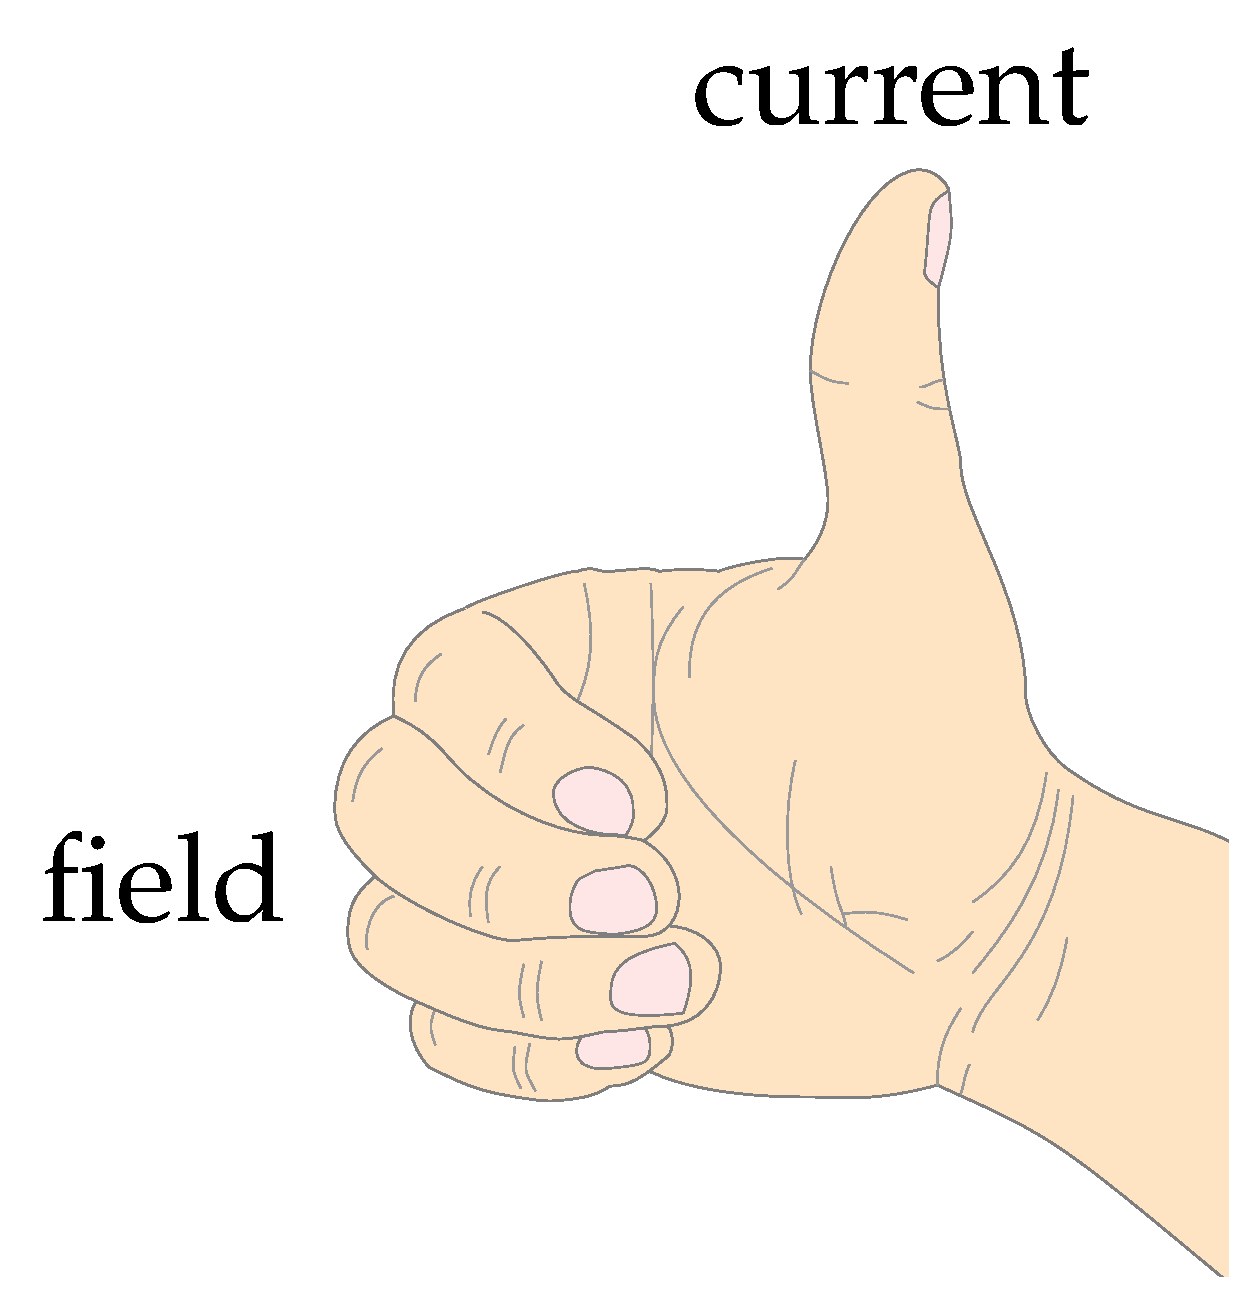
\includegraphics[height=108pt]{right-hand-straight.pdf}
\end{center}
\end{minipage}

\caption{The field due to a long straight current-carrying wire}
\end{figure}

\begin{figure}[ht]
	\centering
\begin{minipage}{0.3\linewidth}
	\begin{center}
		\begin{tikzpicture}[scale=0.9,decoration={markings,mark=at position 0.75 with {\arrow{>}}}]
		\draw[very thick, postaction={decorate}] (0,0) ellipse (1.0 and 0.5);
		\draw (1.6,-0.5) node {current};
		\draw[white,fill] (-0.15,0.4) rectangle (0.15,0.6);
		\draw[white,fill] (-0.6,0.3) rectangle (-0.4,0.5);
		\draw[white,fill] (0.6,0.3) rectangle (0.4,0.5);
		\draw [very thick, blue, postaction={decorate}] (0,-2.4) -- (0,-0.7) (0,0) -- (0,2);
		\draw [very thick, blue, postaction={decorate}] (0.96,-2.4) [out=120,in=-84] to (0.54,-0.7) (0.5,0) [out=90,in=-110] to (0.9,2);
		\draw [very thick, blue, postaction={decorate}] (-0.96,-2.4) [out=60,in=-96] to (-0.54,-0.7) (-0.5,0) [out=90,in=-70] to (-0.9,2);
		\draw [very thick, blue, dashed] (0,-0.7) -- (0,-0.1);
		\draw [very thick, blue, dashed] (0.54,-0.7) [out=96,in=-90] to (0.5,0);
		\draw [very thick, blue, dashed] (-0.54,-0.7) [out=84,in=-90] to (-0.5,0);
		\draw (1.4,1.5) node {field};
		\end{tikzpicture}
	\end{center}
\end{minipage}
\begin{minipage}{0.4\linewidth}
	\begin{center}
		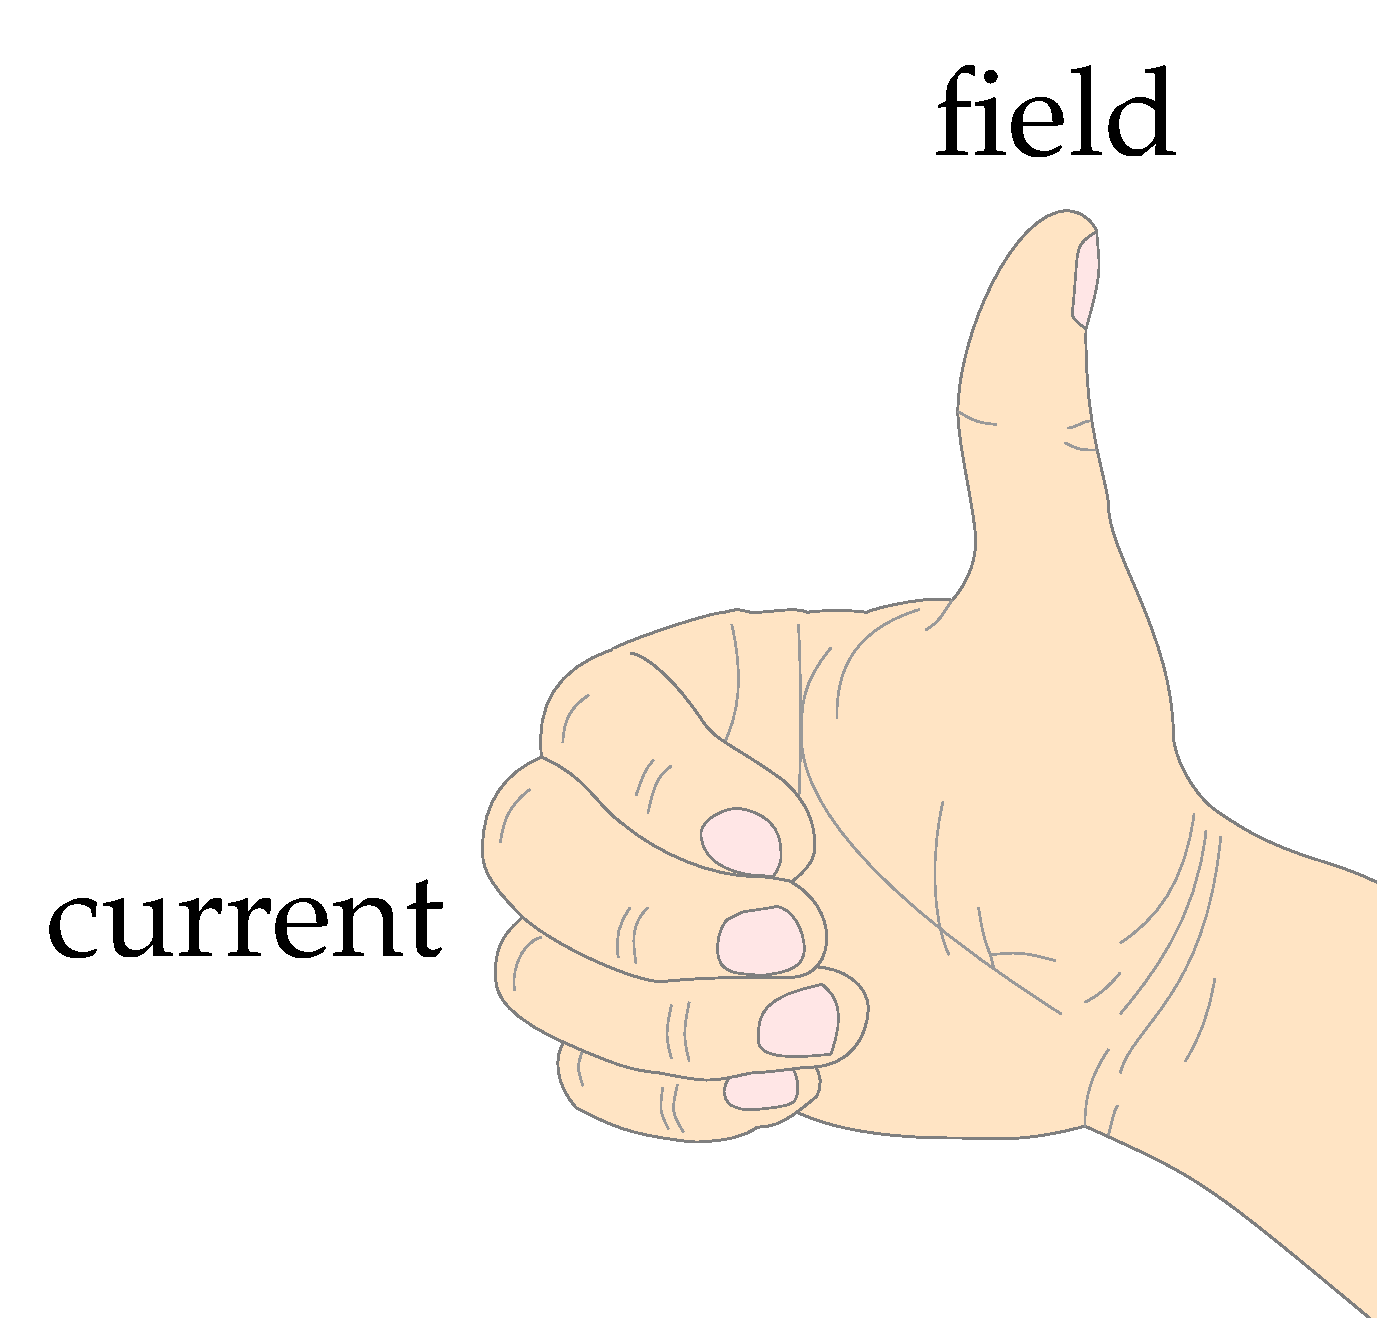
\includegraphics[height=120pt]{right-hand-circular.pdf}
	\end{center}
\end{minipage}

\caption{The field due to a circulating current}
\end{figure}

The strength of the field is proportional to the current: $B \propto I$ for both wires and coils, greater current means stronger field. The magnetic flux density generated by a current flowing in an infinitely long wire in free space is given by: $$\tcbhighmath{B=\frac{\mu_0 I}{2\pi r}}$$
Where:\\
$I$ is the electric current,\\
$r$ is the perpendicular distance from the current, and \\
$\mu_0 = 4\pi \times 10^{-7} \text{ T m A}^{-1}$ is a fundamental physical constant called the \emph{permeability of free space}.

The magnetic flux density at the centre of a current-carrying coil in free space is given by: $$\tcbhighmath{B=\frac{\mu_0 NI}{L}}$$, \\
where:\\
$N$ is the number of turns,\\
$I$ is the electric current flowing through the coil, \\
$L$ is the length of coil, and \\
$\mu_0$ is the permeability of free space.
 
 
\cmt strength of magnetic field can be increased with \emph{soft iron}

this is because \emph{ferromagnetic materials} (iron, cobalt, nickel) can attract magnetic field lines\footnote{If the straight wire is immersed in a material with \emph{relative permeability} $\mu_r$, then the field becomes: $B=\frac{\mu_0 \mu_r I}{2\pi r}$. Similarly, if a material with relative permeability $\mu_r$ is present, then the magnetic flux density inside a coil becomes: $B=\frac{\mu_0 \mu_r NI}{L}$. A good magnetic material (high permeability material), such as iron, has large $\mu_r$, and therefore can greatly intensify the magnetic field. \piste}

\subsection{Solenoids \& electromagnets}

The strength and polarity of the field due to a coil can be changed easily by changing the current, so coils are widely used to create magnetic fields where needed. A current-carrying coil is also called a \keypoint{solenoid}.

\begin{figure*}[htp]
	\centering
	\begin{minipage}{0.65\linewidth}
		\begin{center}
			\begin{tikzpicture}[yscale=0.6,xscale=0.7]
			\tikzstyle flines=[thick,blue,postaction={decorate},decoration={markings,mark=at position 0.56 with {\arrow{>}}}] % field line style
			\tikzstyle ct=[very thick,postaction={decorate},decoration={markings,mark=at position 0.54 with {\arrow{>}}}] % coil style
			
			\draw [flines] (3,0) -- (6.8,0);
			\draw [flines] (3,0.2) [out=10,in=210] to (6.5,1.35);
			\draw [flines] (3,-0.2) [out=-10,in=-210] to (6.5,-1.35);
			\draw [flines] (3,0.5) [out=20,in=240] to (6,3.5);
			\draw [flines] (3,-0.5) [out=-20,in=-240] to (6,-3.5);
			
			\draw [flines] (3,0.9) [out=60,in=0] to (0,3.6) [out=180,in=120] to (-3,0.9);
			\draw [flines] (3,-0.9) [out=-60,in=0] to (0,-3.6) [out=180,in=-120] to (-3,-0.9);
			\draw [flines] (2.5,1) [out=150,in=30] to (-2.5,1);
			\draw [flines] (2.5,-1) [out=-150,in=-30] to (-2.5,-1);
			\draw[ct] (-2.6,-3.5) --++ (0,3);
			
			\draw[thick,fill=white] (3,0) ellipse (0.35 and 1);
			\draw[thick,white,fill] (-3,-1) rectangle (3,1);
			\draw[thick,fill=white] (-3,0) ellipse (0.35 and 1);
			\draw[thick] (-3,-1) -- (3,-1);
			\draw[thick] (-3,1) -- (3,1);
			\foreach \k in {-2.5,-2.0,...,2.1} {\draw[ct] (\k,1) [out=60, in=-120] to (\k+0.4,-1);}
			\draw[very thick] (2.5,1) [out=60, in=-120] to (2.9,-1);
			\draw[white,fill] (2.6,-.978) rectangle (2.8,0);
			\draw[white,fill] (2.7,-1.1) rectangle (2.9,-1.022);
			\draw[very thick] (2.7,0.1) -- (2.7,-1);
			\draw[ct] (2.7,-1) --++ (0,-2.5);
			
			\draw [flines] (-6.8,0) -- (-3,0);
			\draw [flines] (-6.5,1.35) [out=-30,in=170] to (-3,0.2);
			\draw [flines] (-6.5,-1.35) [out=30,in=190] to (-3,-0.2);
			\draw [flines] (-6,3.5) [out=-60,in=160] to (-3,0.5);
			\draw [flines] (-6,-3.5) [out=60,in=200] to (-3,-0.5);
			
			\draw (2.8,-2.1) --++ (1.2,-0.8) node[below]{current};
			\node at (5.4,1.2) {field};
			\node at (3.6,1.4) {N};
			\node at (-3.6,1.4) {S};
			\end{tikzpicture}
		\end{center}
	\end{minipage}
	\begin{minipage}{0.3\linewidth}
		\begin{center}
		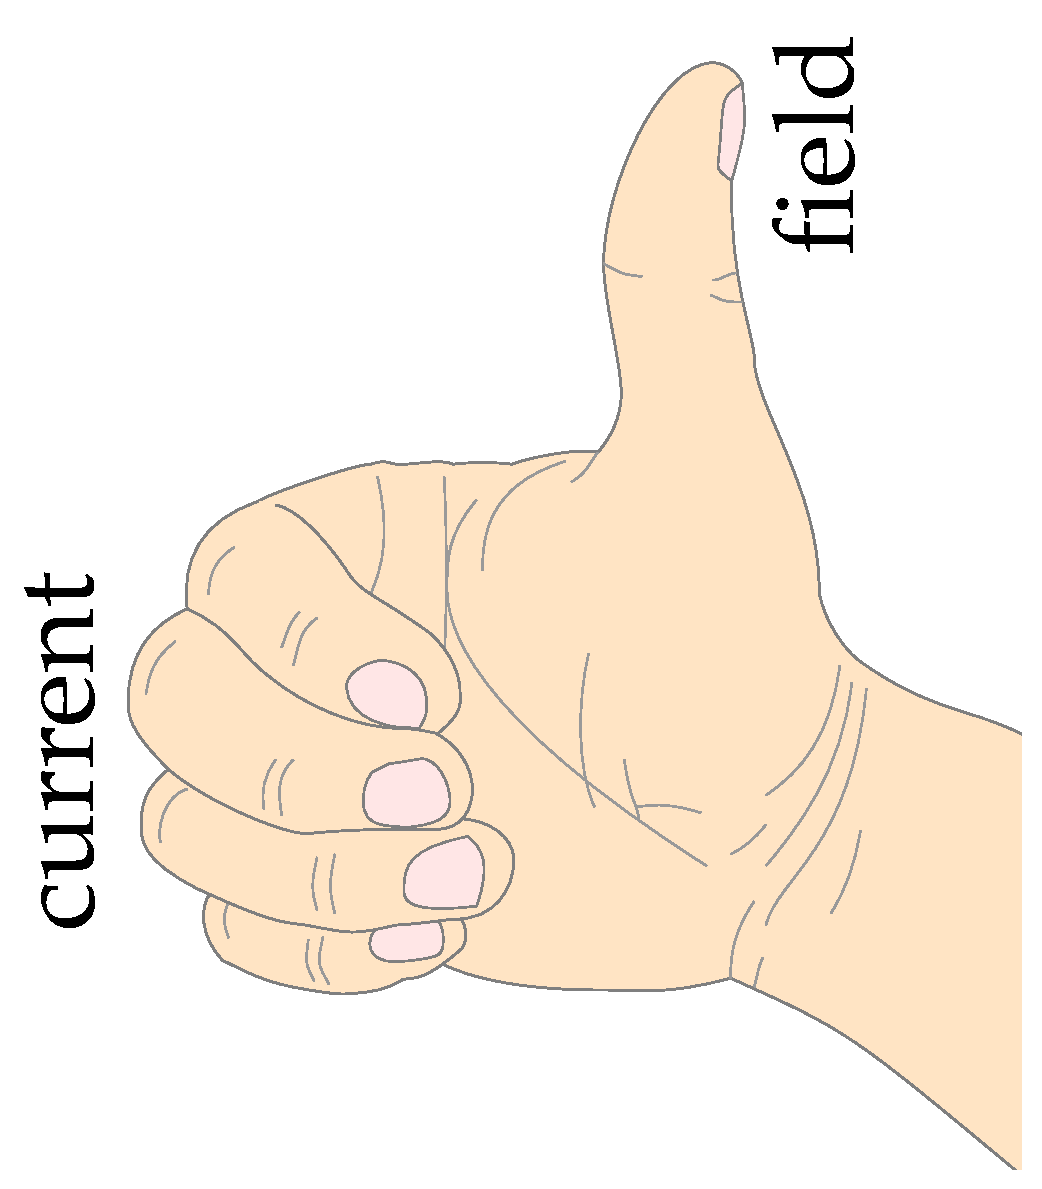
\includegraphics[height=120pt,angle=-90]{right-hand-coil.pdf}
		\end{center}
	\end{minipage}
	
	\caption{The magnetic field around a solenoid}
\end{figure*}

A solenoid generates a magnetic field identically to that of a bar magnet of the same flux density. It's useful to be able to identify the north and south poles of a solenoid. The direction of magnetic field in a solenoid is given by the \keypoint{right-hand (grip) rule}\index{right-hand rule}. Inside the solenoid is a \emph{uniform} magnetic field in its centre. The magnetic field produced by a solenoid can be easily controlled. As current $I\up \ra $ stronger field, also number of turns $N\up\ra $ stronger field. Inserting an \emph{iron core} inside greatly strengthens the field, and  makes an \emph{electromagnet} from a solenoid.

\subsection{Magnetic force on current-carrying conductor}

A current-carrying wire produces its own magnetic field. When it is surrounded by an external magnetic field, the two fields would interact to produde a \keypoint{magnetic force}\index{magnetic field!magnetic force} on the conductor.

\begin{marginfigure}
	\vspace*{-16pt}
	\centering
	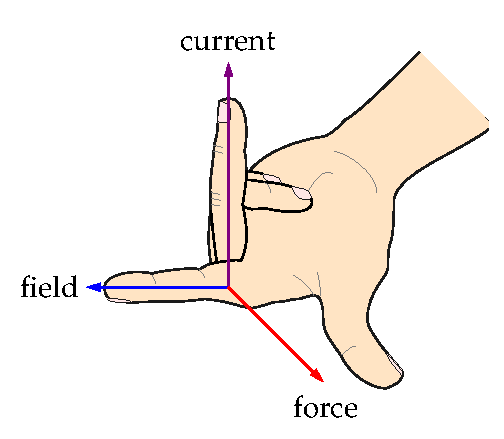
\includegraphics[height=135pt]{left-hand.pdf}
	
	Fleming's left-hand rule
	\vspace*{-16pt}
\end{marginfigure}

The direction of magnetic force on current can be worked out with \keypoint{Fleming's left-hand rule}\index{left-hand rule}\footnote[][2cm]{Figure credit again goes to \emph{Thomas S\"{o}ll} from the CTAN community.}

The magnitude of magnetic force is calculated by: $$\tcbhighmath{F=BIL\sin\theta}$$

$B$ is the magnetic flux density to be specified later

$I$ is the current, $\theta$ is the angle between $B$ and $I$

\cmt when $B \perp I$, magnetic force $F=BIL$

when $B \parallelslant I$, there is no magnetic force

when $B$ forms angle $\theta$ with $I$, only the \emph{perpendicular component} contributes to the force, giving rise to the $\sin\theta$ factor in the formula. The magnetic force is perpendicular to both $B$ and $I$.
\footnote{Vector form of the formula: $\vec{F} = l\vec{I} \times \vec{B}$. \piste}

\begin{center}
	\begin{minipage}[b]{0.32\textwidth}
		\centering
		\begin{tikzpicture}[scale=0.45]
		\foreach \y in {-2,2} \foreach \x in {-2,2}
		\node at (\x,\y) {\large\textcolor{blue}{$\times$}};
		%magnetic fields
		\draw[ultra thick,->] (-3.5,0) -- (2,0) node[below]{\textcolor{black}{$I$}} ;
		\draw[ultra thick] (2,0) -- (3.5,0); %currents
		\draw[red,very thick,->] (0,0) -- (0,2.4) node[right]{$F$};
		\node[blue,above right] at (2,2) {$B$};
		\end{tikzpicture}
		
		(a)
	\end{minipage}
	\begin{minipage}[b]{0.32\textwidth}
		\centering
		\begin{tikzpicture}[scale=0.4]
		\foreach \y in {-2,2} \foreach \x in {-2,2}
		\draw[blue,fill] (\x,\y) circle(0.1);
		%magnetic fields
		\draw[ultra thick,->] (0,-3.5) -- (0,2) node[right]{\textcolor{black}{$I$}} ;
		\draw[ultra thick] (0,2) -- (0,3.5); %currents
		\draw[red,very thick,->] (0,0) -- (2.4,0) node[below]{$F$};
		\node[blue,above right] at (2,2) {$B$};
		\end{tikzpicture}
		
		(b)
	\end{minipage}
\begin{minipage}[b]{0.32\textwidth}
	\centering
	\begin{tikzpicture}[scale=0.64,decoration={markings,mark=at position 0.84 with {\arrow{>}}}]
	\foreach \y in {-2,2}
	{
		\draw[blue,thick,postaction={decorate}] (-3,\y) -- (3,\y);
	}
	%magnetic fields
	\node[blue] at (3.4,1) {$B$};
	\draw [very thick, postaction={decorate}] (-2,0) -- ++(0:4) node[right] {$I$};
	\node[red,below] at (0,-0.3) {$F=0$};
	\end{tikzpicture}
	
	(c)
\end{minipage}
\end{center}

\subsection{Magnetic flux density} \label{sec:magnetic_flux_density}

If we rewrite $F=BIL\sin\theta$ as $B = \frac{F}{IL\sin\theta}$,we can now give a formal definition for flux density $B$:

\begin{ilight}
	\keypoint{Magnetic flux density}\index{magnetic field!magnetic flux density} $B$ at a point is defined as the force acted per unit length on a conductor carrying a unit current at right angle to the magnetic field.
\end{ilight}

Flux density describes the strength of a magnetic field\footnote{Magnetic field strength is a different quantity, defined by $H=\frac{B}{\mu}$, with $\mu=\mu_0\mu_r$ being the \emph{magnetic permeability} of material. The naming of field strength $H$ and flux density $B$ are due to historical reasons.}

\cmt $B$ is measured in \keypoint{tesla}\index{tesla} (T)\footnote{Telsa is a very large unit. For example, the strength of a typical refrigerator magnet is of about $10^{-3} \text{ T}$, even the very strong superconducting coils used in MRI are of around $1\sim3 \text{ T}$.}: $[B]=\text{T}$, $1 \text{ T} = 1 \text{ N}\cdot\text{A}^{-1}\cdot\text{m}^{-1}$

\begin{ilight}
	If a wire of 1 m normal to the magnetic field that carries a current of $1\text{ A}$ experiences a force of $1\text{ N}$, then the magnetic flux density is $1\text{ T}$
\end{ilight}

\cmt $B$ is a \emph{vector} quantity, with both magnitude and direction

	

\newpage

\begin{marginfigure}
	\vspace*{-12pt}
	\centering
	\begin{tikzpicture}[scale=0.96,decoration={markings,mark=at position 0.75 with {\arrow{>}}}]
	\draw[very thick, postaction={decorate}] (0,0) -- (0,3);
	\draw[very thick, postaction={decorate}] (0,3) -- (2,3);
	\draw[very thick, postaction={decorate}] (2,3) -- (2,0);
	\draw[very thick,postaction={decorate}] (0.8,-1.4) -- (0.8,0) -- (0,0);
	\draw[very thick,postaction={decorate}] (2,0) -- (1.2,0) --++ (0,-1.4);
	\foreach \y in {0.5,2.5} {
		\draw[blue,thick,->] (-1,\y) -- (3,\y);
	}
	\node[above,blue] at (3,2.5) {$B$};
	\node[below left] at (0,0) {$P$};
	\node[above left] at (0,3) {$Q$};
	\node[above right] at (2,3) {$R$};
	\node[below right] at (2,0) {$S$};
	\node[right] at (2,1) {$I$};
	\node[right,red] at (2.1,1.5) {$F$};
	\node[left,red] at (-0.1,1.5) {$F$};
	
	\draw[thick,<->] (-1.5,0) --++ (0,3) node[left, midway]{$L$};
	\draw[thick,<->] (0,3.6) --++ (2,0) node[midway,above]{$d$};
	
	\draw[white,fill] (2,1.5) circle (0.18);
	\draw[white,fill] (0,1.5) circle (0.18);
	\draw[red,thick] (2,1.5) circle (0.18);
	\draw[red,thick,fill] (2,1.5) circle (0.06) (0.6,1.3) node[above right]{$I$};
	\draw[red,thick] (0,1.5) circle (0.18);
	\draw[red,very thick] (-0.1,1.4) -- (0.1,1.6) (-0.1,1.6) -- (0.1,1.4);
	\end{tikzpicture}
	\vspace*{-8pt}
\end{marginfigure}

\begin{marginfigure}
	\vspace*{-12pt}
	\centering
	\begin{tikzpicture}[scale=0.75]
	\draw[ultra thick] (-2.5,0) -- (-2.5,4) --++ (1,0) --++ (0,-3) --++ (3,0) --++ (0,3) -- (2.5,4) -- (2.5,0) -- cycle;
	\node at (0,4) {\large $\otimes$};
	\node[above] at (0,4.1) {$I$};
	\node at (2,3.6) {$N$};
	\node at (-2,3.6) {$S$};
	\draw[ultra thick] (-3,-2) rectangle (3,-0.1);
	\draw[thick] (-1.5,-1.6) rectangle (1.5,-0.5);
	\node at (0,-1.1) {\large 500.0 g};
	\end{tikzpicture}
	\vspace*{-12pt}
\end{marginfigure}

\label{ex-mag-balance}

\subsection*{The force between long straight current-carrying wires}

\begin{center}
\begin{minipage}{0.3\linewidth}
\begin{center}
\begin{tikzpicture}[scale=0.84,decoration={markings,mark=at position 0.6 with {\arrow{>}}}]
\draw[ultra thick, postaction={decorate}] (-1.2,0) node[left]{$I_1$} (-1.2,-2) -- (-1.2,2);
\draw[ultra thick, postaction={decorate}] (1.2,0) node[right]{$I_2$} (1.2,-2) -- (1.2,2);
\end{tikzpicture}
\end{center}
\end{minipage}
\begin{minipage}{0.35\linewidth}
\begin{center}
\begin{tikzpicture}[scale=0.56,decoration={markings,mark=at position 0.4 with {\arrow{>}}}]
\draw[black,thick] (0,0) circle (0.25);
\draw[black,thick,fill] (0,0) circle (0.06) (0,0.2) node[above]{$I_1$};
\draw[black,thick] (3,0) circle (0.25);
\draw[black,thick,fill] (3,0) circle (0.06) (3,0.2) node[above left]{$I_2$};
\draw[thick, blue, postaction={decorate}] (4:3) arc [radius=3, start angle=5, end angle=356];
\draw[blue] (144:3.6) node{$B_1$};
\draw[red,thick,->] (3,0) -- (1.2,0) node[below]{$F_{21}$};
\end{tikzpicture}
\end{center}
\end{minipage}
\begin{minipage}{0.3\linewidth}
\begin{center}
\begin{tikzpicture}[scale=0.84,decoration={markings,mark=at position 0.6 with {\arrow{>}}}]
\draw[ultra thick, postaction={decorate}] (-1.2,0) node[left]{$I_1$} (-1.2,-2) -- (-1.2,2);
\draw[ultra thick, postaction={decorate}] (1.2,0) node[right]{$I_2$} (1.2,-2) -- (1.2,2);
\draw[red,thick,->] (1.2,0) -- (0.1,0) node[below right]{$F_{21}$};
\draw[red,thick,->] (-1.2,0) -- (-0.1,0) node[below left]{$F_{12}$};
\end{tikzpicture}
\end{center}
\end{minipage}
\end{center}

If we have two straight parallel wires carrying currents in the same direction then the force acting on $I_2$ is due to magnetic field $B_1$ generated by $I_1$. From the top view, $I_1$ creates a counter-clockwise $B_1$, so $I_2$ experiences an upward field.

Using left-hand rule, the force acting on $I_2$ by $I_1$, denoted $F_{21}$\footnote{$F_{AB}$ denotes the force acted on object $A$ by object $B$.}, points to the left. Since $F_{21}$ and $F_{12}$ are a pair of action-reaction, so $F_{12}$ points to the right.

\begin{center}
\begin{minipage}{0.3\linewidth}
\begin{center}
\begin{tikzpicture}[scale=0.84,decoration={markings,mark=at position 0.6 with {\arrow{>}}}]
\draw[ultra thick, postaction={decorate}] (-1.2,0) node[left]{$I_1$} (-1.2,-2) -- (-1.2,2);
\draw[ultra thick, postaction={decorate}] (1.2,0) node[right]{$I_2$} (1.2,2) -- (1.2,-2);
\end{tikzpicture}
\end{center}
\end{minipage}
\begin{minipage}{0.35\linewidth}
\begin{center}
\begin{tikzpicture}[scale=0.56,decoration={markings,mark=at position 0.4 with {\arrow{>}}}]
\draw[black,thick] (0,0) circle (0.25);
\draw[black,thick,fill] (0,0) circle (0.05) (0,0.2) node[above]{$I_1$};
\draw[black,thick] (3,0) circle (0.25);
\draw[black,thick] (3,0.2) node[above left]{$I_2$};
\draw[black,thick] (3.13,0.13) -- (2.87,-0.13) (3.13,-0.13) -- (2.87,0.13);
\draw[thick, blue, postaction={decorate}] (4:3) arc [radius=3, start angle=5, end angle=356];
\draw[blue] (144:3.6) node{$B_1$};
\draw[red,thick,->] (3,0) -- (4.8,0) node[below]{$F_{21}$};
\end{tikzpicture}
\end{center}
\end{minipage}
\begin{minipage}{0.3\linewidth}
\begin{center}
\begin{tikzpicture}[scale=0.84,decoration={markings,mark=at position 0.6 with {\arrow{>}}}]
\draw[ultra thick, postaction={decorate}] (-1.2,0) node[right]{$I_1$} (-1.2,-2) -- (-1.2,2);
\draw[ultra thick, postaction={decorate}] (1.2,0) node[left]{$I_2$} (1.2,2) -- (1.2,-2);
\draw[red,thick,->] (1.2,0) -- (2.2,0) node[below left]{$F_{21}$};
\draw[red,thick,->] (-1.2,0) -- (-2.2,0) node[below right]{$F_{12}$};
\end{tikzpicture}
\end{center}
\end{minipage}
\end{center}

Similar discussions apply for $I_1$ and $I_2$ flowing in opposite directions (left as exercise for the reader).

So we come to a conclusion: \emph{parallel currents attract, and anti-parallel currents repel}\footnote{The S.I. unit for current, ampere, was defined using two long wires parallel to each other carrying the same current in the same direction. If the wires are separated by 1 m and the magnetic force experienced per metre is $2.0\times10^{-7}$ N, then the current is of 1 A.}

\label{q-pwires}

\begin{figure}[htp]
\centering
\begin{tikzpicture}[scale=1.2,decoration={markings,mark=at position 0.65 with {\arrow{>}}}]
\draw[very thick, postaction={decorate}] (0,0) --++ (0,4) node[pos=0.55, left]{$I_1$};
\draw[very thick, postaction={decorate}] (3,0) --++ (0,4) node[pos=0.55, left]{$I_2$};
\draw[gray,dashed,thick] (-2.5,1) --++ (1.5,2) --++ (6.5,0) --++ (-1.5,-2) --++ (-6.5,0); 
\end{tikzpicture}
\end{figure}

\begin{compactenum}
\item[(a)] Draw at least three lines to show the magnetic field due to $I_1$.

\item[(b)] State and explain the direction of force acting on $I_2$.

\item[(c)] Given that $I_1$ and $I_2$ are separated by 4.0 cm, what is flux density due to $I_1$ at $I_2$?

\item[(d)]  What is the magnetic force per unit length acting on $I_2$?

\item[(e)] What is the magnitude and the direction of the force per unit length acting on $I_1$?
	
\end{compactenum}

\subsection{Magnetic force on charged particles}

Electric currents are formed by moving charges, since current-carrying wires in a magnetic field experience force, charged particle moving in magnetic field should also experience force

\subsection{Magnetic force on charged particles}

Starting from $F=BIl\sin\theta$, let's substitute $I=nAqv \RA F=B(nAqv)l\sin\theta$. Note that $n$ is the number density of charged particles, so $nAl$ together gives the total number of charged particles. If we look at the force acting on \emph{one} charged particle, then $nAl=1$, so: $F=Bqv\sin\theta$\index{magnetic field!magnetic force}

The magnitude of magnetic force on charged particle then is: $$\tcbhighmath{F=Bqv\sin\theta}$$

Where:\\
$B$ is magnetic flux density, \\
$q$ is electric charge of the particle,\\
$v$ is its velocity\\
$\theta$ refers to the angle between $B$ and $v$\\

\begin{marginfigure}
	\vspace*{-16pt}
	\centering
	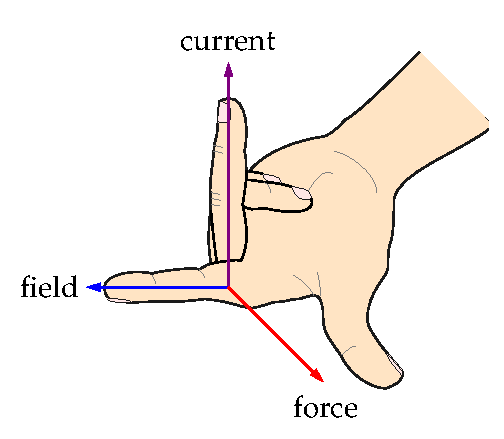
\includegraphics[height=135pt]{left-hand.pdf}
	
	Fleming's left-hand rule
	\vspace*{-16pt}
\end{marginfigure}

The direction of magnetic force can be determined using \emph{Fleming's left-hand rule}\index{left-hand rule}.\\
for $+q$, current in same direction as $v$\\
for $-q$, current in opposite direction as $v$\\

\cmt The force depends on \emph{perpendicular component} of $B$\\ 
If $v \perp B$, magnetic force $F=Bqv$.

If $v \parallelslant B$, there is no magnetic force.

When a particle moves at angle $\theta$ to $B$, the contribution to the force only comes from the \emph{perpendicular component}, giving rise to the $\sin\theta$ factor. the magnetic force always perpendicular to both velocity $v$ and magnetic field $B$.\footnote{Vector form of the formula: $\vec{F} = q\vec{v} \times \vec{B}$. \piste}

\begin{figure*}
	\begin{minipage}[b]{0.45\textwidth}
		\centering
		\begin{tikzpicture}[scale=1]
		\draw[blue,dashed] (-2.7,-2.7) rectangle (2.7,2.7);
		\foreach \y in {-2,0,2} \foreach \x in {-2,0,2}
		\node at (\x,\y) {\large\textcolor{blue}{$\times$}};
		%magnetic fields
		\draw[purple,very thick,->] (-1.1,-1.2) --++ (1.5,0) node[midway,above]{$v$};
		\draw[red,very thick,->] (-1.1,-1.2) --++ (0,1.8) node[left]{$F$};
		\shade [ball color = orange] (-1.1,-1.2) circle (0.15);
		\node[below] at (-1.1,-1.4) {$+q$};
		\draw[purple,very thick,->] (1.2,1.2) --++ (0,-1.5) node[midway,right]{$v$};
		\draw[red,very thick,->] (1.2,1.2) --++ (-1.8,0) node[above]{$F$};
		\shade [ball color = green] (1.2,1.2) circle (0.15);
		\node[above] at (1.2,1.4) {$-q$};
		\node[blue,above right] at (2,2) {$B$};
		\end{tikzpicture}
		
		(a)
	\end{minipage}
	\begin{minipage}[b]{0.45\textwidth}
		\centering
		\begin{tikzpicture}[scale=1]
		\draw[blue,dashed] (-2.7,-2.7) rectangle (2.7,2.7);
		\foreach \y in {-2,0,2} \foreach \x in {-2,0,2}
		\draw[blue,fill] (\x,\y) circle(0.05);
		%magnetic fields
		\draw[purple,very thick,->] (-0.6,-1.2) --++ (110:1.4) node[midway,above right]{$v$};
		\draw[red,very thick,->] (-0.6,-1.2) --++ (20:1.8) node[below]{$F$};
		\shade [ball color = orange] (-0.6,-1.2) circle (0.15);
		\node[below] at (-0.6,-1.4) {proton};
		\draw[purple,very thick,->] (1,0.5) --++ (70:1.2) node[midway,right]{$v$};
		\draw[red,very thick,->] (1,0.5) --++ (160:1.8) node[above]{$F$};
		\shade [ball color = green] (1,0.5) circle (0.15);
		\node[below] at (1,0.3) {electron};
		\node[blue,above right] at (2,2) {$B$};
		\end{tikzpicture}
		
		(b)
	\end{minipage}
\end{figure*}

\subsection*{Charged particles in electric \& magnetic fields}

In either electric field or magnetic field, charged particle may experience a force\footnote{The combination of electric and magnetic force on the charge due to electromagnetic fields is called the \emph{Lorentz force}\index{Lorentz force}: $\vec{F} = q(\vec{E} + \vec{v}\times \vec{B})$. If you have a good knowledge in maths, everything we cover in this section can be recovered from this vector equation. \piste}, in this section, we will compare the difference between electric field and magnetic field:

\begin{center}
	{%\renewcommand{\arraystretch}{1.2}
		\begin{tabular}{|D{0.22\textwidth}|D{0.36\textwidth}|D{0.3\textwidth}|}
			
			\hline
			& electric field & magnetic field \\ \hline
			
			strength of the field & electric field strength $E$ & magnetic flux density $B$ \\ \hline
			
			magnitude of force & $F_E = Eq$ & $F_B=Bqv\sin\theta$ \\ \hline
			
			whether force depends on velocity & no dependence, acts equally on stationary or moving charges & depend on perpendicular component of velocity \\ \hline
			
			\multirow{2}{*}{direction of force} & $F_E \parallelslant E$ &  $F_B \perp B$ and $F_B \perp v$ \\
			
			& same as/opposite to $E$ for $+q$/$-q$ & use left-hand rule\\ \hline
			
			effect of force on motion of particle & can change both magnitude and direction of velocity & only changes direction of velocity, cannot change magnitude of velocity \\ \hline
			
			work done by force & work can be done, can define notions of potential and P.E. & magnetic force does no work for charged particles\\ \hline
			
	\end{tabular}}
\end{center}

\subsection{Charged particle in uniform magnetic fields}

Suppose a charged particle is moving at right angle to a uniform magnetic field:

\begin{figure}[htp]
	\centering
	\begin{tikzpicture}[scale=0.65]
			\draw[blue, dashed] (-4,-4) rectangle (4,4);
			\foreach \x in {-3,0,3}{
				\foreach \y in {-3,0,3}{
					\node[draw,circle,blue,inner sep=0.8pt,fill] at (\x,\y) {};  }}
			\node[blue] at (-2.5,2.5) {$B$};
			\draw[thick,dotted] (0,0) circle [radius=2.5];
			\foreach \s in {80,200,310}
			{
				\draw [purple, thick, ->] (\s:2.5) -- ++(\s-90:2);
				\draw [purple] (\s-35:3.5) node{$v$};
				\draw [red, thick, ->] (\s:2.5) -- (\s:0.8);
				\draw [red] (\s+25:1) node{$F$};
				\shade [ball color = yellow] (\s:2.5) circle (0.25) node{\footnotesize$+$};
			}
	\end{tikzpicture}
	
	\caption{Circular motion of a charged particle in uniform magnetic field}
\end{figure}

The magnetic force $F_B$ is always at right angle to motion, so $F_B$ keeps changing the direction of velocity. A uniform field means a constant force, so $F_B$ deflects the particle at the same rate and the particle describes a \emph{circular} path.

\begin{ilight}
	For a charged particle moving in a uniform magnetic field, \emph{magnetic force provides centripetal force for circular motion}: $\tcbhighmath{Bqv = \frac{mv^2}{r}}$, or $\tcbhighmath{Bqv = m \omega^2 r}$
\end{ilight}

We can solve for radius of the orbiting particles: $r=\frac{mv}{Bq}$

\begin{compactenum}

\item[-] $v\up \Rightarrow r\up$, faster particles take larger circles
	
\item[-] $B\up \Rightarrow r\down$, stronger magnetic field, larger centripetal force, smaller circles
	
\item[-] $m\up \Rightarrow r\up$, larger mass, larger inertia, so larger circles

\end{compactenum}
	
The radius of curvature relates to charge-to-mass ratio (also called \emph{specific charge}\index{specific charge}) of the particle. If we rearrange the equation we have $\frac{q}{m}=\frac{v}{Br}$, which can be computed using experimental data.

	
\subsection{The mass spectrometer}

A \keypoint{mass spectrometer}\index{mass spectrometer} is a device to measure the charge-to-mass ratio of charged particles.

\begin{figure*}[ht]
	\centering
	\begin{tikzpicture}[scale=0.72,decoration={markings,mark=at position 0.7 with {\arrow{>}}}]
	% electric fields
	\draw[orange,dashed,fill=orange!20] (-8,1.5) rectangle (-4,-1.5);
	\draw[ultra thick] (-8,-1.5) --++ (0,3);
	\draw[ultra thick] (-4,-1.5) --++ (0,1.3) (-4,1.5) --++ (0,-1.3);
	\draw (-6,-1) --++ (-1.2,-1.5) node[twoline,below]{accelerating voltage\\supply of p.d. $V$};
	% magnetic field
	\draw[dashed,blue,fill=blue!10] (0,1) rectangle (5,-9);
	\node[blue] at (3.6,-0.4){$B$};
%	\foreach \y in {0.167,-1.5,-3.167,-4.833,-6.5,-8.167} \foreach \x in {0.833,2.5,4.167}
%	\node[blue] at (\x,\y) {$\times$};
	\draw (4.5,-0.5) --++ (1.2,1.2) node[twoline,right]{uniform magnetic\\field region};
	% paths of particle beam
	\draw [thick,purple,postaction={decorate}] (0,0) arc(90:-90:4);
	\draw [thick,purple,postaction={decorate}] (0,0) arc(90:-90:3);
	\draw [thick,purple,postaction={decorate}] (-8,0) -- (-4,0);
	\draw [thick,purple,postaction={decorate}] (-4,0) -- (0,0);
	\node[purple,above] at (-2,0) {$v$};
	\shade [ball color = green] (-7,0) circle (0.2);
	\shade [ball color = green] (-3,0) circle (0.2);
	\draw[<->] (-0.3,0) --++ (0,-8) node[midway,left]{$d=2r$};
	% detectors
	\draw[gray!50,fill] (-1,-5) rectangle(-0.7,-9);
	\draw (-0.85,-6.5) --++ (-1,1) node[left,twoline]{particle\\detector};
	\end{tikzpicture}
	
	\caption{deflection of two charged particles in a mass spectrometer}
\end{figure*}

In use, charged particles are accelerated through an electric field: $\frac{1}{2}mv^2 = qV$, they then enter a uniform magnetic field: $Bqv = \frac{mv^2}{r} \ra v=\frac{Bqr}{m}$.\\

Eliminating $v$: $v^2 = \frac{2qV}{m} = \frac{B^2 q^2 r^2}{m^2} \ra \frac{q}{m} = \frac{2V}{B^2 r^2}$\\

We can then measure $V$, $B$, $r$ in practice, so the charge-to-mass ratio $\frac{q}{m}$ is worked out. Since different particles usually have different values of $\frac{q}{m}$, so this technique is widely used to identify unknown particles.

\subsection{The cyclotron}\index{cyclotron}

A \keypoint{cyclotron} is a type of \emph{particle accelerator.}

\begin{figure}[ht]
	\centering
	\begin{tikzpicture}[decoration={markings,mark=at position 0.6 with {\arrow{>}}}, scale=1.12]
	\def\gap{0.6}
	% magnetic fields
	\draw[thick, dashed, blue, fill=blue!10] (-2.6,0) arc(180:25:2.73) [out=-25, in = 100] to (10:3.2) arc(10:0:3.2) --cycle;
	\draw[thick, dashed, blue, fill=blue!10] (-2.6,-\gap) arc(180:360:2.9) -- cycle;
	% electric field
	\draw[thick, dashed, blue, fill=orange!20] (-2.6,0) rectangle (3.2,-\gap);
	% semi-circular paths
	\draw[thick, postaction={decorate}] (1,0) arc(0:180:1);
	\draw[thick, postaction={decorate}] (-1,-\gap) arc(180:360:1.414);
	\draw[thick, postaction={decorate}] (1.818,0) arc(0:180:1.732);
	\draw[thick, postaction={decorate}] (-1.636,-\gap) arc(180:360:2);
	\draw[thick, postaction={decorate}] (2.364,0) arc(0:180:2.236);
	\draw[thick, postaction={decorate}] (-2.108,-\gap) arc(180:360:2.449);
	% accelerating paths
	\foreach \x in {1.818,2.364,2.791} \draw[thick, postaction={decorate}] (\x,-\gap) --++ (0,\gap);
	\foreach \x in {-1, -1.636, -2.108} \draw[thick, postaction={decorate}] (\x, 0) --++ (0,-\gap);
	\draw[thick, postaction={decorate}] (2.791,0) --++(0,3);
	\draw[thick] (1,-\gap/2) --++(0,\gap/2);
	% proton source
	\draw[fill] (1,-\gap/2) circle(0.1);
	% nodes
	\draw (0.207, -\gap) ++ (200:2.6) -- (-4,0.8) (160:2.3) -- (-4,1) node[left,twoline]{magnetic field\\into the paper};
	\draw (-2.4,-\gap/2) -- (-3.6,-1) node[left,twoline]{high-frequency\\alternating\\electric field};
	\draw (1,-\gap/2) -- (3.2,-2.8) node[right,twoline]{proton\\source};
	\draw (2.791,2.2) -- (1,3.5) node[above, twoline]{outgoing beam of\\high-speed protons};
	\end{tikzpicture}
	
	\caption{Protons being accelerated in a cyclotron}
\end{figure}

The idea is to makes use of magnetic force to guide moving charges into a spiral path between accelerations by an electric field, as the particle enters and leaves the region of electric field, it gains extra energy of $qV$. The particle then follows a semi-circular path under magnetic force and re-enters the electric field. At this point the polarity of the electric field is reversed so the particle continues to accelerate across the gap and the energy of particle increases by $qV$, it then moves in a larger semi-circle in magnetic field. This process is repeated many times until the particle leaves the exit port with very high speed.
For charged particles circulating in a uniform magnetic field: $Bqv=m\omega^2 r$ and the time to complete one full turn is: $T=\frac{2\pi r}{v} = \frac{2\pi}{v}\times\frac{mv}{Bq}\ra T=\frac{2\pi m}{Bq}$.

Rather magically, this shows the period is independent of radius of the circular path!

If an alternating voltage is applied at frequency $f=\frac{Bq}{2\pi m}$, the particles can be accelerated continuously as they cross the gap at just the right time. This frequency is known as the \emph{cyclotron frequency}.

\subsection{Velocity selector}

A \keypoint{velocity selector}\index{velocity selector} is a device to produce a beam of charged particles all with same speed $v$.

\begin{figure}[ht]
	\centering
	\begin{tikzpicture}[xscale=0.9,yscale=0.8]
	\foreach \x in {-2,2}
	\foreach \y in {-1.5,1.5}
	\node[blue] at (\x,\y) {$\times$};
	\foreach \x in {-3,-1,...,3}
	\draw[orange,thick,->] (\x,3) -- (\x,-3);
	\node[blue] at (-2,2.1) {$B$};
	\node[orange] at (3.5,-2) {$E$};
	\draw[ultra thick] (-4,3) -- (4,3);
	\draw[ultra thick] (-4,-3) -- (4,-3);
	\draw[ultra thick] (0,-4.5) node[right]{$-$} -- (0,-3) (0,3) -- (0,4.5) node[right]{$+$};
	\draw [fill] (-4.2,0.2) rectangle (-4,3.6);
	\draw [fill] (-4.2,-0.2) rectangle (-4,-3.6);
	\draw [fill] (4.2,0.2) rectangle (4,3.6);
	\draw [fill] (4.2,-0.2) rectangle (4,-3.6);
	\shade [ball color = green] (-6.5,0) circle (0.1);
	\node[below,twoline] at (-6.5,-0.2) {electron\\beam};
	\draw[purple,thick,->] (-6.2,0) -- (-5,0) node[above,midway]{$v$};
	\draw[purple,thick,->] (-5,0) -- (6,0) node[above]{$v=\frac{E}{B}$};
	\draw[purple] (-4,0) [out=0,in=210] to (4,2);
	\node[purple,right] at (4.2,2) {$v<\frac{E}{B}$};
	\draw[purple] (-4,0) [out=0,in=160] to (4,-1.5);
	\node[purple,right] at (4.2,-1.5) {$v>\frac{E}{B}$};
	\shade [ball color = green] (0,0) circle (0.1);
	\draw[red,thick,->] (0,0.2) -- (0,2) node[above]{\textcolor{black}{$F_E=Eq$}};
	\draw[red,thick,->] (0,-0.2) -- (0,-2) node[below]{\textcolor{black}{$F_B=Bqv$}};
	
	\end{tikzpicture}
	
	\caption{A velocity selector in action.}
\end{figure}

Let's consider a beam of electrons passing through a region where both uniform electric field and magnetic field are applied, electrons at the desired speed $v$ are \emph{undeflected}, there's no net force acting on these electrons, so there is equilibrium between electric and magnetic force:

{

\centering

$F_E = F_B \RA Eq = Bqv \RA \tcbhighmath{v=\frac{E}{B}}$

}

For particles entering the same region with higher speed, $F_B>F_E$, they deflect upwards, for particles entering the same region with lower speed, $F_B<F_E$, they deflect downwards.

\subsection{Hall effect}
The Hall effect is a really neat application of the interaction of charged particles and fields. When an electric current passes through a conductor surrounded by an external magnetic field perpendicular to the current, a transverse potential difference is produced. This phenomenon \index{Hall effect} was discovered by American physicist \emph{Edwin Hall} in 1879, the voltage difference is called the \keypoint{Hall voltage}.

\vspace*{\baselineskip}

Suppose magnetic field is aligned upward, and the current flows to the right (see figure \ref{hallsens1}), then the charge carriers (assumed to be electrons for now) experience a magnetic force pointing to the bottom left of the page.

\begin{figure}[ht]
	\centering
	\begin{tikzpicture}[scale=1]
	\draw[thick] (-6,.5) -- ++(3,0); % current in
	\draw[thick,fill=gray!20] (-4,-1) -- ++(0,1) -- ++(3,2) -- ++(4,0) -- ++(0,-1)  -- ++(-3,-2) -- cycle;
	\draw[thick] (-4,0) -- (0,0) -- (3,2) (0,0) -- (0,-1); %conductor
	\draw[blue,thick,->] (-.5,-2.5) -- (-.5,-1) (-.5,1) -- ++(0,2) node[right]{$B$}; %magnetic fields
	\draw[thick,->] (1.5,.5) -- ++(3,0) node[above]{$I$}; % current out
	\shade [ball color = green] (-1.1,1) circle (0.12);
	\draw[thick,purple,->] (-1.1,1) -- ++(-1,0) node[above right]{$v$};
	\draw[thick,red,->] (-1.1,1) -- ++(-1,-.667) node[left]{$F_B$};
	\end{tikzpicture}
 \caption{Hall sensor fig 1}
 \label{hallsens1}
\end{figure}

This magnetic force causes a build-up of extra charge on front side of conductor, which produces an internal electric field $E$ inside conductor, i.e., a potential difference $V_H$ is formed.

\begin{figure}[ht]
	\centering
	\begin{tikzpicture}[scale=1]
	\draw[thick] (-6,.5) -- ++(3,0); % current in
	\draw[thick,fill=gray!20] (-4,-1) -- ++(0,1) -- ++(3,2) -- ++(4,0) -- ++(0,-1)  -- ++(-3,-2) -- cycle;
	\draw[thick] (-4,0) -- (0,0) -- (3,2) (0,0) -- (0,-1); %conductor
	\draw[blue,thick,->] (-.5,-2.5) -- (-.5,-1) (-.5,1) -- ++(0,2) node[right]{$B$}; %magnetic fields
	\draw[thick,->] (1.5,.5) -- ++(3,0) node[above]{$I$}; % current out
	\shade [ball color = green] (-1.1,1) circle (0.12);
	\draw[thick,purple,->] (-1.1,1) -- ++(-1,0) node[above right]{$v$};
	\draw[thick,red,->] (-1.1,1) -- ++(-1,-.667) node[left]{$F_B$};
	\draw[thick,violet,->] (-1.1,1) -- ++(1,.667) node[right]{$F_E$};
	\foreach \ball in {-3.5,-2.5,-1.5,-0.5}{
		\shade [ball color = green] (\ball,-0.5) circle (0.12);
		\draw[thick] (\ball-0.05,-0.5) --++ (0.1,0);
	}
	\draw[thick,olive,<->] (-4.8,0) -- ++(3,2) node[midway,above left]{$V_H$};
	\draw[thick,olive,<-] (-0.8,.3) node[left]{$E$} -- ++(2.1,1.4);
	\draw[thick,<->] (.5,-1.35) -- ++(3,2) node[midway, below right]{$d$};
	\draw[thick,<->] (3.5,1) -- ++(0,1) node[midway, right]{$t$};
	\end{tikzpicture}
 \caption{Hall sensor fig 2}
 \label{hallsens2}
\end{figure}

As the charge carriers accumulate on one side, the Hall voltage opposes further migration of charges, so a steady $V_H$ is established when magnetic force and electric force are balanced: $Eq = Bqv$.

\begin{compactenum}
	\item[-] strength of internal electric field is related to Hall voltage: $E=\frac{V_H}{d}$
	
	where $d$ is width of the conductor
	
	\item[-] drift velocity $v$ of particles is related to current $I$: $I=nAqv$
	
	where $A$ is cross section of conductor and $n$ is number density of charge carriers
\end{compactenum}

we now have: $\frac{V_H}{d}q = Bq \frac{I}{nAq} \ra V_H = \frac{BId}{nAq}$

note that cross section $A=dt$, where $t$ is thickness of conductor as shown

we therefore obtain an useful expression for Hall voltage: $$ V_H = \frac{BId}{n(td)q} \ra \tcbhighmath{V_H = \frac{BI}{ntq}}$$ 

To produce a noticeable $V_H$, we want smaller $n$ and smaller $t$

\begin{compactenum}
	\item[-] $n\downarrow \ra$ few free charge carriers $\ra$ \emph{semi-conductors} are preferable

	\item[-] $t\downarrow \ra$ small thickness $\ra$ \emph{thin slice} of component is preferable

\end{compactenum}

The polarity of $V_H$ is determined by nature of charge carries. The charge carriers can be \emph{free electrons} (negatively charged) or \emph{holes} (positively charged), these would obviously cause the Hall voltage to have opposite polarity.

% If current $I$ forms angle $\theta$ with flux density $B$, again only perpendicular component matters

% expression for Hall voltage becomes: $V_H = \frac{BI}{ntq}\sin\theta$
	
\cmt apply a fixed current in a conductor, $V_H$ is proportional to $B$
	
 % so magnetic flux density can be calculated once we find $V_H$
	
% one can make use of Hall effect to build a \emph{Hall probe}, a device used to measure flux density $B$

% when using a Hall probe, one should rotate and record the greatest voltage reading to ensure the current applied is at right angle to the external magnetic field

\cleardoublepage

% ===== Chapter: 27-electromagnetic-induction =====
\chapter{Electromagnetic Induction}

\subsection{Magnetic flux}

\rcyskip

\begin{ilight}
	\keypoint{magnetic flux} is defined as the product of a closed area and the magnetic flux density going through it at right angles: $$\tcbhighmath{\phi=BA\cos\theta}$$\index{magnetic field!magnetic flux}
\end{ilight}

\begin{marginfigure}
	\centering
	\begin{tikzpicture}[scale=1.25]
	
	\foreach \y in {-1.5,-0.75,0,0.75,1.5} \draw[blue,thick] (-1.5,\y-.6) -- (0,\y);
	\draw[very thick, fill=gray!25] (0,0) ellipse (0.6 and 1.2);
	\node at (-0.2,0.3) {$A$};
	\foreach \y in {-1.5,-0.75,0,0.75,1.5} \draw[blue,thick,->] (0,\y) -- (1.5,\y+0.6);
	\draw[thick,dashed] (0,0) -- ++(1.5,0);
	\draw[thick] (.8,0) arc(0:21.8:0.8);
	\draw (0,0) ++ (10.5:1) node {$\theta$};
	\node[blue] at (1.7,1) {$B$};
	\end{tikzpicture}
\end{marginfigure}

\cmt The unit for magnetic flux: $[\phi] = \text{Wb}$, $1\text{ WB} = 1 \text{ T}\cdot\text{m}^2$

If magnetic field is perpendicular to the area then
magnetic flux simply becomes: $$\tcbhighmath{\phi=BA}$$

For a coil with $N$ turns, total magnetic flux is:

{

\centering

$\tcbhighmath{\Phi = N\phi = NBA}$

}

This is called \keypoint{magnetic flux linkage}. Graphically this can be thought of as the number of field lines through area $A$. If the loop cuts theough field lines this means a change in flux.

A change in flux can be caused by many processes, for example:

\begin{compactenum}
	\item[-] moving a magnet towards/away from a coil
	
	\item[-] varying current in a solenoid/electromagnet
	
	\item[-] inserting an iron core into a solenoid/electromagnet
	
	\item[-] pushing a straight conductor through a magnetic field
	
	\item[-] rotating a coil in a magnetic field
	
	\item[-] $\cdots$
\end{compactenum}

\subsection{Laws of electromagnetic induction}

Electromagnetic induction is the phenomena that magnetism produces electricity\index{electromagnetic induction}. The laws of electromagnetic induction were discovered by \emph{Michael Faraday} and \emph{Heinrich Lenz} in the 1830s, and later described mathematically by \emph{James Clerk Maxwell}. We will study the conditions under which voltages and currents could be induced, and how to find their magnitudes and polarities.

\subsection{Faraday's law}

\rcyskip

\begin{ilight}
	\keypoint{Faraday's law}\index{Faraday's law} states that induced e.m.f./voltage is proportional to rate of change in magnetic flux (linkage): $$\tcbhighmath{\mathcal{E} \propto \frac{\Delta \Phi}{\Delta t}}$$
\end{ilight}

\cmt Faraday's law gives the \emph{magnitude} of the induced e.m.f. - the key here is the \emph{change} in flux: as long as flux changes, e.m.f. will be induced.

If $\mathcal{E}$, $\Phi$, $t$ are all given in SI units, this proportional relation becomes: $$\tcbhighmath{\mathcal{E} = -\frac{\Delta \Phi}{\Delta t}}$$

\subsection{Lenz's law}

\rcyskip

\begin{ilight}
	\keypoint{Lenz's law}\index{Lenz's law} states that induced e.m.f. or current is always in the direction to produced effects that \emph{oppose} the change in flux that produced it.
\end{ilight}

\cmt Lenz's law gives the \emph{polarity} of the induced current - the key here is the nature ``dislikes'' any change in flux: effects of induced current always \emph{oppose} the cause of its production. Lenz's law is a consequence of the conservation of energy, since induced current dissipates electrical energy as heat, it must cause loss of original forms of energy possessed by the system. If the change in flux is caused by motion, then magnetic force on/by the induced current must \emph{resist} this motion.

\begin{figure}[ht]
	\centering
		\begin{circuitikz}[european resistors, scale=0.72]
		\tikzstyle ct=[thick] % coil style
		\draw[thick,fill=white] (3,0) ellipse (0.35 and 1);
		\draw[thick,white,fill] (-3,-1) rectangle (3,1);
		\draw[thick,fill=white] (-3,0) ellipse (0.35 and 1);
		\draw[thick] (-3,-1) -- (3,-1);
		\draw[thick] (-3,1) -- (3,1);
		\foreach \k in {-2.5,-2.0,...,2.1} {\draw[ct] (\k,1) [out=60, in=-120] to (\k+0.4,-1);}
		\draw[ct] (2.5,1) [out=60, in=-120] to (2.9,-1);
		\draw[white,fill] (2.6,-.978) rectangle (2.8,0);
		\draw[white,fill] (2.7,-1.1) rectangle (2.9,-1.022);
		\draw[ct] (-2.6,-1) -- (-2.6,-3.5) to[R=$R$] (2.7,-3.5) -- (2.7,0);
		
		\draw [fill=blue!70] (-9,-0.5) rectangle (-7.5,0.5);
		\draw [fill=red] (-7.5,-0.5) rectangle (-6,0.5);
		\node at (-8.25,0) {\large \textcolor{white}{S}};
		\node at (-6.75,0) {\large \textcolor{white}{N}};
		\draw[ultra thick, blue,->,dashed] (-5.5,0) -- (-3.5,0);
	\end{circuitikz}
\end{figure}

\noindent (a) What is average induced e.m.f. in the coil? (b) What is average induced current through resistor $R$? (c) In which direction does this current flow?

\newpage

\label{ex-cuttingFL}

\begin{figure}[ht]
	\centering
	\begin{circuitikz}[european resistors, scale=0.9]
		\draw[thick] (0,1) --++ (10,0);
		\draw[thick] (-1,-1) --++ (10,0);
		\draw[ultra thick, gray] (-1,-1.5) -- (0.5,1.5);
		\draw[ultra thick,->,red] (-0.25,0) --++ (1.5,0) node[midway,above]{$v$};
		\draw[<->] (-1.5,-1) -- (-0.5,1) node[midway,above,rotate=63.43]{$L$};
		\foreach \x in {2,4,6,8} \draw[->,thick, blue] (\x,-2.4) -- (\x,-1.2) (\x,0) --++(0,2);
		\node[blue] at (6.5, 2) {$B$};
		\draw (10,1) [out=0,in=75] to (12,1) to[R=$R$] (11,-1) [out=255,in=0] to(9,-1);  
	\end{circuitikz}
\end{figure}

\noindent (a) What is the induced current through resistor? (b) In which direction does this current flow? (c) For the rod to travel at constant speed, what is magnitude of external force required?

% \subsection*{Hall voltage \& induced voltage in a coil}
	
% in this section, we compare readings on voltmeter connected to a Hall probe and a coil
		
% Hall probe picks up voltage proportional to flux density: $V_H \propto B$
		
% coil picks up induced e.m.f. proportional to \emph{rate of change} in flux: $\mathcal{E} \propto \frac{\dd \Phi}{\dd t}$
		
% \question{If a Hall probe is placed near a permanent magnet, what voltage do you measure? If a small coil is placed in the same field, state and explain whether you can measure a non-zero voltage in the coil. If not, state three different ways in which you can produce a voltage.}

% \begin{marginfigure}
% 	\centering
% 	\vspace*{-8pt}
% 	\begin{tikzpicture}[xscale=0.8,yscale=0.7]
% 		\draw[<->] (0,3) node[left]{$I$} -- (0,0) -- (6,0) node[below]{$t$};
% 		\draw (0,-2) -- (0,0);
% 		\draw[thick,blue] (0,0) [out=70, in=180] to (2,2) -- (3.5,2) -- (3.8,-1.6) -- (6,-1.6);
% 	\end{tikzpicture}
% 	\vspace*{-20pt}
% \end{marginfigure}

% \question{A Hall probe is placed near one end of a solenoid that carries a varying current as shown in the graph. (a) Sketch the variation of Hall voltage with time. (b) If Hall probe is replaced by a small coil parallel to the solenoid's end, sketch the variation of the voltage induced in the coil.}

\section{Applications of electromagnetic induction}

\subsection{Magnetic braking}

Induction brakes make use of induced current to dissipate kinetic energy of a moving object. We will look at two simple demonstrations, but the principle can be used in braking system of high-speed trains, roller-coasters, etc.

\subsection*{The damped pendulum}

A metal disc can swings freely between the poles of an electromagnet, when the electromagnet is switched on, the disc comes to rest very quickly.

\begin{figure}[ht]
\centering
\begin{tikzpicture}[scale=0.6]
% disc
\draw [thick] (0,6) ++ (-120:6) ++ (0,0.1) --++ (60:6) arc(150:-30:0.1) --++ (240:6);
\draw [thick,fill=gray!50] (0,6) ++ (-120:6) circle (1.2);
\draw [very thick, gray,dashed] (0,6) ++ (-60:6) circle (1.2);
\draw [purple,very thick,dashed,<->] (0,6) ++ (-75:6) arc(-75:-105:6);
% poles of EM magnet
\draw[thick] (0,1) rectangle (3,2.5);
\draw[thick] (-3,-1) -- (0,-1) -- (0,-2.5);
\draw[thick] (0,2.5) --++ (30:3);
\draw[thick] (3,2.5) --++ (30:2.7);
\draw[thick] (3,1) --++ (30:3);
\draw[thick] (-3,-1) --++ (210:3);
\draw[thick] (0,-1) --++ (210:4);
\draw[thick] (0,-2.5) --++ (210:3);
% nodes
\draw (3,1.75) ++(30:0.8) --++ (-30:2.5) node[twoline,below right]{poles of an\\electromagnet};
\draw (0,-1.75) ++(210:0.8) --++ (16:6.2);
\draw (0,6) ++ (-120:6) ++ (-0.5,0) --++ (150:3) node[left]{metal disc};
\end{tikzpicture}

%oscillation of pendulum dies away quickly due to drag force on eddy currents
\end{figure}

As the disc moves in and out of field, change in flux gives rise to e.m.f induced. Note that different parts of the disc experience different rates of change in flux, different e.m.f. is induced in different parts for the disc, this causes circulating currents flowing in the disc, called \keypoint{eddy currents}.

\begin{compactenum}
	\item[-] vibrational energy is lost as heat due to the eddy currents induced
	
	\item[-] magnetic force on induced current causes damping
\end{compactenum}

so amplitude of oscillation decreases quickly

\subsection*{Falling magnet}

Suppose we drop two strong magnets down a plastic tube and a copper tube;

\begin{figure}[ht]
	\centering
	\begin{tikzpicture}[scale=0.7]
	\draw[thick] (-2,0) ellipse (1 and 0.4) ellipse (0.9 and 0.36);
	\draw[thick] (-2,-5) ellipse (1 and 0.4);
	\draw[white,fill] (-3,-5) rectangle (-1,-4.5);
	\draw[thick] (-3,0) -- (-3,-5) (-1,0) -- (-1,-5);
	\draw[thick] (2,0) ellipse (1 and 0.4) ellipse (0.9 and 0.36);
	\draw[thick] (2,-5) ellipse (1 and 0.4);
	\draw[white,fill] (3,-5) rectangle (1,-4.5);
	\draw[thick] (3,0) -- (3,-5) (1,0) -- (1,-5);
	\draw[thick,fill=gray!30] (-2.4,1) rectangle (-1.6,3);
	\draw[thick,fill=gray!30] (2.4,1) rectangle (1.6,3);
	\draw (-2,2.4) -- (-0.5,4) (2,2.4) -- (0.5,4) (0,4) node[twoline, above]{strong\\magnets};
	\draw (-2,-3) --++ (-2.5,1) node[left,twoline]{plastic\\tube};
	\draw (2,-3) --++ (2.5,1) node[right,twoline]{copper\\tube};
	\end{tikzpicture}
	
	%it takes much longer for magnet to fall through copper tube
\end{figure}

as magnet falls, tube experiences change in flux, so e.m.f is induced. Since plastic is an insulator, so no current flows in plastic tube, magnet undergoes free fall, but in the conducting copper tube, eddy current is induced in the tube.

\begin{compactenum}
	\item[-] energy is lost as heat due to induced current, not all G.P.E. converted into K.E.
	
	\item[-] induced current exerts magnetic force on magnet to oppose its motion, acceleration $a<g$
\end{compactenum}

so the magnet falls more slowly through the copper tube.

\begin{marginfigure}
\centering
\begin{circuitikz}[european resistors,scale=0.75]
	% spring and magnet
	\draw[ultra thick] (-1,3.5) -- (1,3.5);
	\draw[thick, decorate, decoration={coil,amplitude=4pt, segment length=5pt}] (0,3.5) -- (0,1.5);
	\draw[thick, fill=gray!30] (-0.3,-0.5) rectangle (0.3,1.5);
	\draw[thick, fill=white] (-1,0) rectangle (1,-3.1);
	% coil
	\foreach \y in {-0.4,-0.7,...,-2.6} {
		\draw[thick] (-1,\y+0.1) [out=200, in=20] to (1,\y-0.1);
	}
	% circuit
	\draw[thick] (-1,-2.7) [out=200, in=180] to (0,-2.8) -- (1,-2.8) to[R=$R$] (3.6,-2.8);
	\draw[thick] (1,-0.2) -- (2,-0.2) --++ (30:0.7) (2.7,-0.2) -- (3.6,-0.2) -- (3.6,-2.8);
	% labels
	\draw (0,2.5) --++ (1.5,0.8) node[right]{spring};
	\draw (0,1) --++ (1.5,0.8) node[right]{magnet};
	\draw (-0.4,-0.7) --++ (-1.5,0.8) node[left]{coil};
	\node[above] at (2.1,0) {$S$};
\end{circuitikz}

\end{marginfigure}

\subsection{The generator} \label{subsection:generators}

Imagine a coil rotates with constant angular speed $\omega$ in a uniform magnetic field $B$

\begin{marginfigure}
	\vspace*{-8pt}
	\centering
	\begin{tikzpicture}[scale=1,decoration={markings,mark=at position 0.75 with {\arrow{>}}}]
	\draw[very thick,postaction={decorate}] (0,2.1) ellipse (0.5 and 0.2);
	\draw[white,fill] (-0.15,2.1) rectangle (0.15,2.5) node[right]{\textcolor{black}{$\omega$}}; 
	\foreach \y in {-1.2,0,1.2}
	{
		\draw[blue,thick] (-2,\y) -- (-0.8,\y);
		\draw[blue,thick,->] (0,\y) -- (2,\y);
	}
	
	\draw[blue] (1.8,0.6) node{$B$};
	\draw[very thick] (-0.6,-1.8) -- (0.6,-1.2) -- (0.6,1.8) -- (-0.6,1.2) -- cycle;
	\draw[thick,dashed] (0,-2.1) -- (0,2.5);
	\draw[thick,dashed] (0,0) -- (1.2,0.6);
	\draw (0.8,0) arc(0:26.565:0.8);
	\node at (13:1) {$\theta$};
	
	\end{tikzpicture}
 \label{motor1}
 \caption{The generator}
\end{marginfigure}

Let's assume that the coil initially lies in parallel to the field, i.e., $\theta=0$ at $t=0$, at time $t$, coil forms an angle $\theta=\omega t$ with the magnetic field (see diagram \ref{motor1})

The magnetic flux linkage through coil is:

{

\centering

$\Phi = NBA \sin\theta = NBA \sin \omega t$

}

The magnitude of induced e.m.f. is: 

{
	
\centering

$\mathcal{E} = \frac{\dd \Phi}{\dd t} = \omega NBA \cos \omega t$

}

This is a sinusoidal voltage with maximum value: $\mathcal{E}_\tmax = \omega NBA$, for a coil rotating in a magnetic field like this, an \emph{alternating current} is generated. This is basically how a \emph{generator}\index{generator} works.
In practice, it is a strong electromagnet rotating inside a large coil to generate electricity.

\subsection{Electromagnetic gun}

A coil of wire of many turns is wound on a hollow tube over which is placed a light copper ring. The ring can move freely along the tube. Let's find out what happens to the ring when a high-voltage supply is switched on...

\begin{figure}[htp]
\centering
\begin{tikzpicture}[scale=0.75]
% tube base
\draw[fill=white] (0,0) ellipse (2 and 1);
% solenoid
\foreach \idx in {0.8,0.9,...,2} \draw[fill=gray!25] (0,\idx) ellipse (2.4 and 1.2); 
\draw[fill=white] (0,2) ellipse (2 and 1);
\draw[white,fill] (-2,2) rectangle (2,4);
\draw (-2,1.95) --(-2,3.5) (2,1.95) -- (2,3.5); 
% ring
\draw[fill=gray!10] (0,3.5) ellipse (2.4 and 1.2);
\draw[gray!10,fill] (-2.4,3.5) rectangle (2.4,4);
\draw[fill=gray!25] (0,4) ellipse (2.4 and 1.2);
\draw (-2.4,3.45) --(-2.4,4) (2.4,3.45) -- (2.4,4);
% tube top
\draw[fill=white] (0,4) ellipse (2 and 1);
\draw[white,fill] (-2,4) rectangle (2,6);
\draw (-2,3.95) --(-2,5.5) (2,3.95) -- (2,5.5);
\draw[fill=gray!25] (0,5.5) ellipse (2 and 1);
% labels
\draw (-1.2,4) --++ (-3,1.2) node[left]{hollow tube};
\draw (-1.2,2.8) --++ (-3,1.2) node[left]{copper ring};
\draw (-1.2,0.5) --++ (-3,1.2) node[left,twoline]{insulated coil};
% circuit
\draw (2.4,1.5) -- (4,1.5) -- (4,2.4) -- (7,2.4) -- (7,1.5);
\draw (2.4,0.9) -- (4,0.9) -- (4,0) -- (7,0) -- (7,0.9);
\draw (7,1.45) circle(0.05);
\draw (7,0.95) circle(0.05);
\node[right,twoline] at (7.2,1.2) {high-voltage\\supply};
\end{tikzpicture}
\end{figure}

When the supply is switched on, the flux density in the coil greatly increases. The sudden change in magnetic flux could induce a huge e.m.f. in copper ring. The resulting induced current in ring would experience a repulsive magnetic force, this repulsive force could be a lot larger that ring's weight, and so the ring would jump up from the tube.

If the ring is replaced by a small metal sphere placed inside the tube, the same strong magnetic force arising from a sudden change in flux could fire the sphere at very high speed...

\subsection*{other applications}

As a final remark, electromagnetic induction is widely used in many other areas as well

for those who are interested, you may research on the principles behind wireless charging, induction cooking, contactless payment technology, smart pencils for tablets or computers, etc.

\cleardoublepage

% ===== Chapter: 29-quantum-physics =====
\chapter{Quantum Physics Basics}

In this chapter, we will study the laws of nature at very small scales.

We start by reviewing classical concepts like particles or waves, and then see how they break down when being applied to the microscopic world. For those observations that could not be explained with classical physics, we need \emph{quantum physics}. The theory of quantum physics is very deep and profound, so surely way beyond the scope of our course. What we will study in this A-Level course are merely four tips of an enormous iceberg, namely

\begin{compactenum}
	\item[-] photon theory / photoelectric effect
	
	\item[-] matter waves / electron diffraction
	
	\item[-] electron energy levels / atomic spectra
	
	\item[-] band theory / electrical conductivity of solids
\end{compactenum}

\subsection{Classical theories}

In classical physics, both particle models and the wave models have been very useful, though both being successful, the two model are distinct in many aspects. To understand a phenomenon, we take either the particle picture or the wave picture. It seems that there is no way in which the particle model would reconcile with wave models...

\subsection{Particle models}

In a particle model, any system is considered to consist of particles governed by \emph{Newtonian mechanics}, physical properties of this system are predicted by newtonian mechanics. Areas of science where particle models are used to interpret and make predictions include:

\begin{compactenum}
	\item[-] \emph{electricity}: electric current formed by motion of charge carriers
	
	\item[-] \emph{ideal gas}: pressure caused by collisions of gas molecules
	
	\item[-] \emph{solid}: elasticity due to interaction between solid atoms
	
	\item[-] \emph{radioactivity}: decay interpreted as the emission of $\alpha$-/$\beta$-particles from the nucleus
	
	\item[-] \emph{chemistry}: chemical reactions due to exchange of electrons between atoms and molecules
	
	\item[-] $\cdots$
\end{compactenum}

\subsection{Wave models}

In the wave picture, energy is transferred via the vibration of medium or force fields. Phenomena that can be explained in terms of wave models include:

\begin{compactenum}
	\item[-] \emph{water waves}: variation in the vertical displacement of water surface
	
	\item[-] \emph{propagation of sound}: variation in the pressure and density of medium
	
	\item[-] \emph{light}: variation of electric and magnetic fields
	
	\item[-] $\cdots$
\end{compactenum}

A key feature that makes waves distinct from particles is that waves can \emph{superpose} - when two or more waves meet, they add up or cancel out to give a resultant wave. This property gives rise to the characteristic behaviour of waves:

\begin{compactenum}
	\item[-] \emph{interference}: waves superpose to form a resultant wave of greater or lower amplitude
	
	\item[-] \emph{diffraction}: bending of waves around obstacles, or spreading out of waves through slits
\end{compactenum}

\subsection{A history of light}

Efforts to understand the nature of light can be traced all the way back to ancient Greeks, lets skip a few of milennia to the 1600's...

Corpuscular theory of light (\emph{Issac Newton}, 1671) - Light rays is comprised of a stream of massless particles called \emph{corpuscles}.

\begin{compactitem}
	\item[--] explains straight-line propagation
	
	\item[--] explains reflection and refraction
	
	\item[--] explains colours of light seen in dispersion in prism (corpuscles have different colours)
\end{compactitem}

The problems with the particle model include:

\begin{compactitem}
	\item[--] does not agree with observations on refraction
	
	\item[--] cannot predict the interference and diffraction of light
\end{compactitem}

Wave theory of light (\emph{Christian Huygens}, 1678) - Light is a wave that transfers energy within a medium known as \emph{aether}.

\begin{compactitem}
	\item[--] follows laws of reflection and refraction
	
	\item[--] explains colours of light (light have different wavelengths)
	
	\item[--] explains interference (Thomas Young's double slit experiment)
	
	\item[--] explains diffraction (Poisson spot experiment)
\end{compactitem}

The only problem is that aether, the medium in which light lives, was experimentally disproved...

Electromagnetic theory (\emph{James Maxwell}, 1865) - Light is an \emph{electromagnetic wave}.
\footnote{\emph{Maxwell's equations} fully describe the behaviour of electric and magnetic fields. Based on the four equations that Maxwell established, he found the vibration of electric and magnetic field can propagate in space as a classical wave. The speed of electromagnetic wave is given by
	
	{
		
		\centering
		
		$c=\frac{1}{\sqrt{\epsilon_0\mu_0}}=\frac{1}{\sqrt{8.85\times10^{-12}\times4\pi\times10^{-7}}} = 3.00 \times 10^8 \mps$,
		
	}
	
	\noindent which is the same as speed of light. This gave Maxwell the intuition that light is an electromagnetic wave.}

\begin{compactitem}
	\item[--] electric and magnetic fields travel through space in the form of waves at speed of light
	
	\item[--] propagation of electromagnetic wave does not require medium, hence no need for aether
	
\end{compactitem}

all behaviour of light known at that time could be explained with Maxwell's theory

so scientists were convinced that light travelled through space as an electromagnetic wave

\subsection{Photon theory}

\subsection{Photoelectric effect}\label{ch-photoelectricity}

Electromagnetic radiation incident upon a metal can cause emission of electrons from the metal surface, this is called \keypoint{photoelectric effect}\index{photoelectric effect}, 
\footnote{Photoelectric effect was first observed in 1887 by \emph{Heinrich Hertz}, who found electrodes illuminated with ultraviolet light create electric sparks. In school labs, one can shine ultraviolet radiation from a mercury lamp onto a zinc plate to cause photo-emission.} the emitted electrons are called \keypoint{photoelectrons}.

Simply put, conduction electrons in metal gain additional energy by absorbing the incoming radiation, if this energy is sufficient for electrons to overcome the electrostatic attraction from the positive metal ions, they break free from the metal surface.

\begin{figure}
	\centering
	\begin{tikzpicture}[scale=1.2]
	\tikzset{photon/.style={thick, decorate, purple, decoration={snake,segment length=0.8cm,amplitude=4pt}}}
	\draw[thick] (-3,-1) -- (-1.5,1) -- (3,1) -- (1.5,-1) -- cycle;
	\foreach \r in {-4,-3.5,-3} \draw[photon,->] (\r,\r+6) --++ (2.7,-2.5);
	\foreach \r in {-0.5,0,0.5} \draw[blue,thick,->] (\r+0.5,-\r) --++ (3,2.5);
	\shade [ball color = green] (0,0) circle (0.1);
	\shade [ball color = green] (-1,0.5) circle (0.1);
	\shade [ball color = green] (0.8,-0.2) circle (0.1);
	\shade [ball color = green] (0.9,0.7) circle (0.1);
	\shade [ball color = green] (1,-0.7) circle (0.1);
	\shade [ball color = green] (-0.5,-0.4) circle (0.1);
	\shade [ball color = green] (-1.9,-0.6) circle (0.1);
	\draw (-1,-0.8) --++ (-1.2,-0.8) node[left]{metal plate};
	\node[twoline] at (-1.2,2.6) {electromagnetic\\radiation};
	\node[twoline] at (1.5,2.7) {electrons\\released};
	\end{tikzpicture}
\end{figure}

\cmt some detailed experimental observations on the photoelectric effect are:

\begin{compactitem}
	\item[--] there exists a minimum \keypoint{threshold frequency}\index{photoelectric effect!threshold frequency} $f_0$ for incident radiation
	
	when $f<f_0$, no electrons released from metal surface
	
	\item[--] emission of electrons is immediate when radiation is incident as long as $f>f_0$
	
	even low-intensity light is effective
	
	\item[--] increasing intensity has no effect on energies of electrons
	
	\item[--] increasing intensity of incident light causes number of photoelectrons emitted to increase
	
	\item[--] increasing radiation frequency increases electron energies
\end{compactitem}

\cmt wave theory of light fails to explain any of these properties, according to wave model:

\begin{compactitem}
	
	\item[--] electrons could gradually build up energies by absorbing wave energy over time
	
	so radiation at any frequency should all work 
	
	
	\item[--] need very intense light to have immediate effect
	
	\item[--] greater intensity mean higher energy, electrons released should have greater K.E.
	
	\item[--] varying frequency of radiation should have no effect on energy of electrons released
\end{compactitem}

photoelectric effect sees the breakdown of the wave model, some new ideas are needed!

\newpage
\section{The Photo-electric Effect}
When electromagnetic radiation of high enough frequency falls on a metal surface, electrons are emitted from the surface.
For most metals, ultraviolet is needed. For some (including sodium, potassium, caesium), light towards the violet end of the spectrum) will release electrons.

 
\subsection{Demonstrating the Photo-electric Effect}

Either using a zinc plate with a gold leaf electroscope (or a coulombmeter)
\begin{figure*}
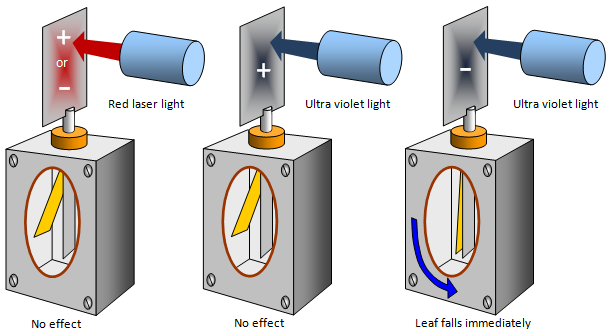
\includegraphics[]{photoelec.png}
\caption{Photoelectric effect demonstrated with electroscope}
\end{figure*}
\begin{itemize}
\item Clean a zinc plate with fine emery paper or steel wool.
\item Attach the plate to the top disc on a gold leaf electroscope, so there is good electrical contact.
\item Charge the zinc plate and inner assembly of the electroscope negatively, e.g. by rubbing the zinc plate with a polythene rod which has been rubbed with wool or fur. The leaf should now be raised, because the leaf and the back plate are both charged negatively and repel each other. The leaf should temporarily rise further if the charged polythene rod is brought near the zinc plate.
\item Place an ultraviolet lamp near the zinc plate. Switch it on. The leaf should be seen to fall. [Safety note: Don't look at the ultraviolet lamp (when it's turned on!)] Clearly the plate (and inner assembly of electroscope) is losing charge.
\item Repeat the procedure, but charging the zinc plate and inner assembly of the electroscope positively, e.g. by rubbing the plate with a charged perspex rod. This time the ultraviolet does not affect the leaf. Charge is not lost.
     \end{itemize}
The simplest explanation is the correct one\ldots The ultraviolet causes electrons to be emitted from the zinc plate. If the plate is charged positively, the electrons are attracted back again. If the plate is charged negatively the emitted electrons are repelled and lost from the plate for ever. 

\subsection{Photo-electric Puzzles}
Before 1905, the energy of a beam of light was thought of as distributed uniformly across broad wavefronts. Calculations showed that it should take some time before an electron in a metal surface could absorb enough energy from the light to escape from the surface. Yet emission is observed as soon as the light falls on the surface.
Another puzzle was why, for a given surface, we find that light of frequency below a certain value (the threshold frequency) causes no electron emission at all.
Einstein's theory of the photo-electric effect solves both these problems\ldots

\subsection{Einstein's Photo-electric Equation}
Although the free electrons in a metal have no allegiance to particular atoms, there are forces `bonding' them to the lattice of ions as a whole. In order to escape from the metal an electron has to do work against these forces. Some have to do more work than others, but there is a certain minimum quantity of work to be done, so no electron can escape unless it is given a certain minimum energy.
The work function, $\phi$, of a metal is the minimum energy needed by an electron in order to escape from the surface. 
Einstein's key idea was that any electron which leaves the surface is ejected by the action of a single photon. Photons don't co-operate in the process.
Recall that a photon of light of frequency $f$ has energy $= hf$. 
Suppose that a photon gives its energy $hf$ to an electron, and that the electron is able to escape. The minimum energy used in escaping is $\phi$, so the maximum kinetic energy the escaped electron can have is what's left over of the photon's energy. So we have the simple equation:
\[ E_{Kinetic} =hf - \phi \]

This assumes that the photon energy is greater than (or equal to) the work function; in other words that  $hf>\phi$ or $f=\phi/h$.
If  $f < \phi/h$, the photon energy will be less than the work function so no electrons at all can escape - a simple explanation of the phenomenon of threshold frequency.
 
The threshold frequency, $f_0$, for a metal is the minimum frequency of electromagnetic radiation needed to produce electron emission from the surface.
From the argument just given, 
\[f_{0} =  \phi/ h.\]
This relationship can also be deduced from Einstein's equation; At the threshold frequency even the most energetic electron will only just manage to escape, so $KE_{max} =  0$, and therefore     $f0 = \phi/h$.
Provided that the light is above the threshold frequency, as soon as it falls on the metal surface electrons will start to be emitted, as emission results from individual photon `hits', and is not a cumulative process as supposed before Einstein.

\subsection{Experimental test of Einstein's Equation}

We use the arrangement with the vacuum photocell shown below  for demonstrating the photoelectric effect.

\begin{figure}
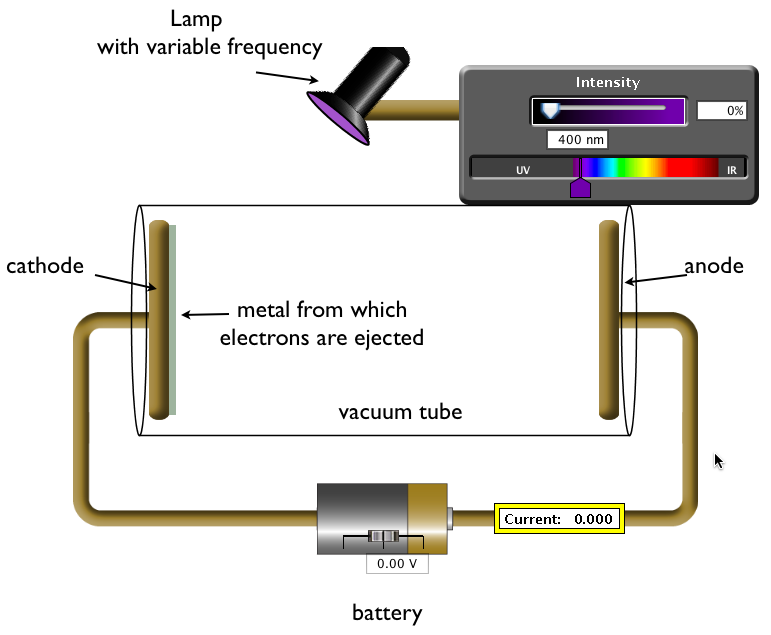
\includegraphics[]{vaccell.png}
\caption{Photoelectric effect with vacuum cell. Note: Picture comes from the fantastic simulation at Phet.}
\end{figure}

\begin{itemize}
\item Use white light with a coloured filter, or a light emitting diode, to illuminate the metal surface with approximately monochromatic light. [Its wavelength can be found using a diffraction grating, hence its frequency, using $f = c / \lambda$ .]
\item Increase the p.d. between the collecting electrode and the metal surface until the current drops to zero. 
At this point the p.d. is called the stopping voltage, $V_{stop}$, because it stops all emitted electrons, even those with the most K.E., from reaching the collector electrode.

\item The maximum K.E. of the emitted electrons is simply given by \sidenote{How do we justify this? Because of the applied voltage, emitted electrons are subject to repulsion by the positive collector electrode and attraction by the emitting surface, hence to a resultant force towards the emitting surface. The electrons therefore get slower and slower as they cross the gap. When the stopping voltage is applied, even the most energetic of emitted electrons have no K.E. left when they have made it across the gap. The K.E. lost is equal to the P.E. gained for these electrons. That's what the equation states.
It is just like finding the K.E. of a ball thrown upwards in the Earth's gravitational field by measuring the its maximum height, and using the energy conservation equation  K.E. lost = mgh}

\[ E_{k} = V_{Stop} \times 1.6 \times 10^{-19} \]

\item Repeat the process using two or three more frequencies of light.
\item Plot a graph of $KE_{max}$ against frequency, $f$. If Einstein's equation is correct it should have a positive slope equal to $h$ and a negative intercept, equal to $ \phi $. We can see this by comparing Einstein's equation with $y = mx + c$.
\begin{align*}
E &= &hf &-& \phi \\
y &= &mx& + &c
\end{align*}
\end{itemize}

A sample graph is presented below.

\begin{figure}
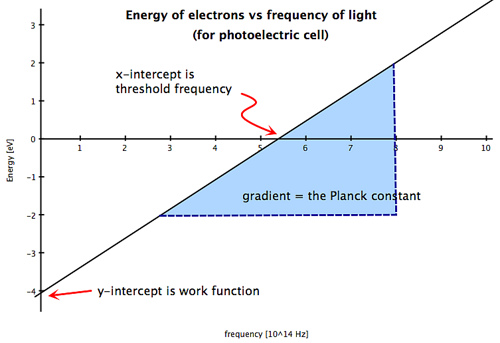
\includegraphics[scale=.6]{photograp.jpg}
\caption{A graph of Frequency vs Kinetic energy}
\end{figure}

It is useful practice to find from the graph:
\begin{itemize}
\item a value of Planck's constant,
\item the threshold frequency for the metal,
\item the threshold wavelength for the metal
\item the work function for the metal
\end{itemize} \sidenote{In practice it is difficult to obtain a good value for h using a commercially available vacuum photocell. Slight impurities on the metal surface (e.g. a thin oxide film), and unwanted electron emission from the collector electrode, both affect the stopping voltage. The first convincing verification of Einstein's photo-electric equation, leading to an accurate value of the Planck constant was completed in 1916 by R.A. Millikan, working in the United States. The secret of his success was a remotely operated knife working in the vacuum to skim off surface layers from the caesium surface as they became contaminated.}
 
\subsection{Effect of changing the Light Intensity}
If we bring a monochromatic light source towards a surface we increase the light energy falling on the surface, per $m^2$, per $s$. We are said to be increasing the intensity of the light. Clearly we can apply the same idea to ultraviolet or any other electromagnetic radiation. We find that:
\begin{enumerate}
\item For light or ultraviolet of a given frequency, changing the intensity has no effect on the maximum K.E. of the emitted electrons. This is exactly what Einstein's theory predicts. The energy given to individual electrons comes from individual photons, and a photon's energy, $hf$, depends only on the frequency (or, equivalently, the wavelength) of the radiation. It doesn't, then, depend on its intensity (provided we don't change the frequency).

\item For light or ultraviolet of a given frequency, increasing the intensity increases the number of electrons emitted per second.
\end{enumerate}
Again, this is just what we'd expect from Einstein's theory. Increasing the intensity means increasing the number of photons arriving at the surface, per m2, per s.  Naturally this means that more electrons will be emitted. \sidenote{Each identical photon has the same probability of emitting an electron.} 
	We can show the effect with the same vacuum photocell arrangement used for demonstrating the photoelectric effect. Note that the polarity of the power supply is arranged to encourage electrons to cross the gap.
    \begin{itemize}
    \item Use a monochromatic light source to illuminate the caesium surface.
\item Check that increasing the p.d. does not affect the current, I. This means that all the electrons emitted per second are being collected.
\item Bring the light source closer and observe the effect on I.
\item I is the charge flowing per second, so the number of electrons emitted per second is I/e in which e is the charge on each electron.
 \end{itemize}

\subsection{Photon theory}

Photoelectric effect was explained by \emph{Albert Einstein} in 1905
\footnote{Albert Einstein was awarded the Nobel Prize in physics in 1921 for `his discovery of the law of the photoelectric effect'. This discovery led to the quantum revolution of modern physics.}

Einstein's revolutionary idea: when radiation delivers energy to matter, the transfer of energy is not continuous but carried in \emph{discrete} packets, called \emph{photons}

\begin{ilight}
	A \keypoint{photon}\index{photon} is a packet (\emph{quanta}) of electromagnetic energy
\end{ilight}

\cmt The energy of one photon is given by: \begin{empheq}[box=\tcbhighmath]{equation*}{E=hf}\end{empheq} 
where $h=6.63\times10^{-34} \text{ J s}$ is the \keypoint{Planck constant}\index{Planck constant}.

Since $E \propto f$, higher/lower radiation frequency means greater/smaller photon energies. The wave equation $c=\lambda f$ relates frequency $f$ of an electromagnetic wave to its wavelength $\lambda$, so the energy of one photon is also given by: \begin{empheq}[box=\tcbhighmath]{equation*}{E=\frac{hc}{\lambda}}\end{empheq}.

Since $E \propto \frac{1}{\lambda}$, longer/shorter wavelength means lower/greater photon energies, the equation $E=hf$, or $E=\frac{hc}{\lambda}$,  relates a particle property to a wave property. $E$ is the energy of one photon, treated like a single particle but $f$ and $\lambda$ are both introduced to describe a wave, not a particle...

The intensity of a beam of radiation is: $I = \frac{P}{A}$ and the total energy incident on a given area per unit time determines the radiation intensity so intensity depends on the product of the number of photons arriving per unit time and energy of each photon: $ \tcbhighmath{I \propto nhf}$, or more precisely, \begin{empheq}[box=\tcbhighmath]{equation*}I = \frac{nhf}{A}\end{empheq}

When considering energy of a photon, \keypoint{electronvolt} is a useful energy unit

one electronvolt (1 eV) is work needed to make an electron travel through a p.d. of 1 V

Conversion between electronvolt and joule is: \begin{empheq}[box=\tcbhighmath]{equation*}{1 \text{ eV} = 1.60\times10^{-19} \text{ J}}\end{empheq}

\label{ex-redlaser}

\subsection{Photoelectric effect explained}

From the viewpoint of photon theory, photoelectric effect can be explained easily. To release an electron from metal, it requires a minimum energy $\Phi$, called the \keypoint{work function}\index{photoelectric effect!work function}, for the electron to overcome attraction due to metal ions to escape from metal surface. 

As radiation shines upon metal, photon energies are absorbed by electrons, since photon energies are \emph{discrete}, or \emph{quantised}, the absorption is sort of all or nothing. If photon energy is greater than $\Phi$, electrons break free from the metal. Excess energy, if any, would become kinetic energy of the free electron.

This is all summarised in \keypoint{Einstein's photoelectric equation}\index{photoelectric effect!photoelectric equation}: 
\begin{empheq}[box=\tcbhighmath]{equation*}{hf = \Phi + E_{k,\tmax}}\end{empheq}

Note that we are talking about \emph{maximum} K.E. of emitted electrons. For electrons to be released from \emph{below} the surface, they require more energy than work function, so less K.E. than maximum value. At the critical point, an incoming photon has just enough energy to release electron, so at threshold frequency\index{photoelectric effect!threshold frequency} $f_0$, photon energy equals work function: \begin{empheq}[box=\tcbhighmath]{equation*}{hf_0 = \Phi}\end{empheq}

Experimental observations mentioned in \S\ref{ch-photoelectricity} can now be understood

\begin{compactitem}
	
	\item[--] below threshold frequency $f_0$, not enough photon energy available to electron to overcome work function, so no effect for $f<f_0$
	
	\item[--] interaction between photon and electron is \emph{one-to-one}, so no time delay
	
	\item[--] greater radiation intensity means more photons per unit time, so more electrons released
	
	\item[--] greater frequency means higher photon energy, so greater K.E. for emitted electron
	
\end{compactitem}

\subsection*{Measurement of the Planck constant and work function energy}

When radiation with different frequencies is incident onto a metal, we measure maximum K.E. of the electrons emitted from the surface, a set of readings $(f, E_{k,\tmax})$ can be found. Note that the photoelectric equation can be rearranged as: $ E_{k,\tmax} = hf - \Phi$

\begin{marginfigure}
	\vspace*{-12pt}
	\centering
	\begin{tikzpicture}[scale=1.2]
	\draw[thick,->] (0,-1.6) -- (0,2.4) node[left]{$E_{k,\tmax}$};
	\draw[thick,->] (0,0) -- (4,0) node[below]{$f$};
	\draw[thick,blue, dashed] (0,-1.2) -- ++(1.6,1.6);
	\draw[thick,blue] (1.6,.4) -- ++(1.8,1.8);	
	\node[left] at (0,-1.2) {$-\Phi$};
	\node[left] at (0,0) {$0$};
	\node[below right] at (1.2,0) {$f_0$};
	\end{tikzpicture}
	\vspace*{-12pt}
\end{marginfigure}

If we plot a graph of $ E_{k,\tmax} $ against $f$, data points shall fall on a straight line, information about the Planck constant $h$, threshold frequency $f_0$, work function $\Phi$ can all be computed with the best-fit line.

\begin{compactitem}
	\item[--] $\text{gradient} = h$
	
	\item[--] $y\text{-intercept} = -\Phi$
	
	\item[--] $x\text{-intercept} = \frac{\Phi}{h} = f_0$	
\end{compactitem}

	
\begin{center}
	\begin{tikzpicture}[scale=0.96]
		\draw[->] (0,-4.5) -- (0,5.5) node[above]{$E_k$/10$^{-19}$J};
		\draw[->] (0,0) -- (10.5,0) node[right]{$f$/10$^{14}$Hz};
		\draw[step=1, gray, very thin] (0,-4) grid (10,5);
		\foreach \x in {0,1,...,10} {
			\draw[white,fill] (\x-0.2,-0.42) rectangle (\x+0.2,-0.08);
			\node[below] at (\x,0) {$\x$};
		}
		\foreach \y in {-4,-3,...,5} \node[left] at (0,\y) {$\y$};
		\node[blue] at (5.0,0.5) {$\times$};
		\node[blue] at (5.8,1.0) {$\times$};
		\node[blue] at (6.7,1.6) {$\times$};
		\node[blue] at (7.6,2.2) {$\times$};
		\node[blue] at (8.4,2.8) {$\times$};
		\node[blue] at (9.5,3.4) {$\times$};
	\end{tikzpicture}
\end{center}
	

\subsection{Photon momentum}

In photoelectric effect, photons can knock electrons out of a metal, this suggests that photons could have \emph{momentum}, even though they do not have mass.

The earliest experimental evidence of photon momentum was came from \emph{Arthur Compton} in 1923, who studied the scattering of X-ray photons by electrons in substances\footnote{Arthur Compton was awarded the Nobel Physics Prize in 1929 for the discovery of this scattering effect, now known as \emph{Compton scattering}.} It can be shown\footnote{This derives from Einstein's theory of \emph{special relativity}, which states that energy and momentum are related by the equation: $E^2 = m_0^2 c^4 + p^2 c^2$. Photons have zero rest mass, i.e., $m_0=0$. This relativistic relation becomes $E=pc$ for photons. Now recall photon energy is given by $E=hf$. Rearrange the terms, we can show: $p = \frac{hf}{c} = \frac{h}{\lambda}$.} that photon momentum is given by: \begin{empheq}[box=\tcbhighmath]{equation*}{p = \frac{h}{\lambda}}\end{empheq}

Photon momentum a \emph{relativistic} momentum, as photons move at speed of light. The definition for classical momentum $p=mv$ does not apply for photons.

However, due to exchange of momentum, electromagnetic waves can exert \emph{radiation pressure}. Forces generated by radiation pressure are negligible under everyday circumstances, but they could have noticeable effects on spacecraft in outer space and comet tails.

\subsection{Wave-particle duality}

\subsection{Matter waves}

Inspired by photon theory, which shows electromagnetic waves have a particulate nature, \emph{Louis de Broglie} suggested in his 1924 PhD thesis that all matter has a wave-like nature
\footnote{Louis de Broglie was awarded the 1929 Nobel Physics Prize `for his discovery of the wave nature of electrons'. \emph{Schr\"oedinger's equation} and \emph{Bohr's atomic model} was heavily influenced by ideas of de Broglie.}

wave characteristic of a particle can be represented by a wavelength

\begin{ilight}
	\keypoint{de Broglie wavelength}\index{de Broglie wavelength} of a matter particle is given by:\begin{empheq}[box=\tcbhighmath]{equation*}{\lambda = \frac{h}{p}}\end{empheq} where $p=mv$ is the particle's momentum
\end{ilight}

 

\subsection{Electron diffraction}

The fact that electrons have wave-like properties was confirmed by \emph{Clinton Davisson} and \emph{George Thomson} in 1927. They showed experimentally electrons could be diffracted\index{electron diffraction} by metal crystals.
\footnote{The Nobel Prize in Physics 1937 was awarded jointly to Clinton Davisson and George Thomson `for their experimental discovery of the diffraction of electrons by crystals'}

\begin{figure}[htp]
	\centering
	\begin{tikzpicture}[scale=1]
	\draw[gray!40,fill] (-0.5,-1) -- (-0.5,0.5) -- (0.5,1) -- (0.5,-0.5) -- cycle;
	\draw[thick,blue,->] (-3,0) -- (-.5,0);
	\draw[gray!20,fill] (5,-3) -- (5,1.5) -- (7,3) -- (7,-1.5) -- cycle;
	\draw[blue, dashed, fill=blue!50, opacity=0.3] (0,0) -- (6,1.2) [out = 0, in=0] to (6,-1.2) --cycle;
	\draw[blue, dashed, opacity=0.3] (6,1.2) [out = 180, in=180] to (6,-1.2);
	\draw[green,fill] (6,0) ellipse (0.06 and 0.12);
	\draw[green,line width=2pt] (6,0) ellipse (0.2 and 0.4);
	\draw[green,line width=2pt] (6,0) ellipse (0.35 and 0.7);
	\draw[green,line width=1.5pt] (6,0) ellipse (0.55 and 1.1);
	\draw (-0.2,-0.5) --++ (-0.5,-1) node[below,twoline]{thin\\crystal};
	\draw (5.5,-2) --++ (2,-0.6) node[below,twoline] {fluoroscent\\screen};
	\draw (6.3,0.9) --++ (2.5,1.5) node[above,twoline] {diffraction pattern\\formed on screen};
	\node[twoline] at (-1.8,0.5) {electron\\beam};
	\end{tikzpicture}
	
	\caption{The electron diffraction experiment}
\end{figure}

If electrons behaved like particles, we would see a round spot of \emph{uniform} distribution, but the actual pattern formed on \emph{fluorescent screen} is a set of \emph{concentric rings}. This is a typical diffraction pattern, and hence this experiment proves the wave properties of electrons. Each metal has a different lattice structure, so each produces a different pattern which in turn allows the investigation of the structure of matter (explore arrangements of atoms, structures of complex molecules, structure of atomic nuclei, etc.) using electron diffraction. Since the wavelength of an electron is much shorter than visible light an \emph{electron microscope} will have much higher resolving power than optical microscopes.

\subsection{Wave-particle duality}

We have seen both particle-like and wave-like behaviour in light and electrons:

\begin{fullwidth}
\begin{center}
	\begin{tabular}{|D{2.5cm}|D{5.5cm}|D{5cm}|}
		\hline
		& electromagnetic radiation & electron \\ \hline
		particle-like & photoelectric effect, & deflection in electric/magnetic \\
		behaviour & radiation 	pressure &  fields, decay, scattering \\  \hline
		wave-like behaviour & interference, diffraction, Doppler
		effect, reflection, refraction & electron diffraction \\ \hline
	\end{tabular}
\end{center}
\end{fullwidth}

When light/electrons move through space, they behave like a wave, however when light/electrons interact with each other, they behave like particles. This two-sided, or \emph{dual} nature of being both a wave and a particle, is described best by either particle model or wave model under different circumstances. All matter (protons, neutrons, atoms, cells, basketballs, human body, earth, etc.) has this universal dual nature, called \keypoint{wave-particle duality}\index{wave-particle duality}. Wave-particle duality addresses breakdown of classical concepts like particle or wave to fully describe the behaviour of microscopic objects, and points us to \emph{quantum mechanics}
\footnote{Being a central concept of quantum theory, wave-particle duality is deeply embedded into the foundations of quantum physics. In non-relativistic quantum mechanics, all information about a particle is encoded in its \emph{wave function}, whose evolution with time is described by the famous \emph{Schr\"odinger's equation}.}

\subsection{Quantisation of electron energy levels}

In a simple atomic model, electrons move around the nucleus in circular orbits, however we understand that electrons have wave properties. As an electron moves in its orbit as a wave, it can superpose with itself. Only orbits in which the electron can superpose constructively with itself can therefore exist. The knock-on implication is that electrons can only take certain values of energy, called \emph{energy levels}.

\subsection{The Hydrogen atom \protect\piste}

The theoretical explanation for electron energy levels was developed in 1913 by Danish physicist \emph{Niels Bohr} in his theory of hydrogen atom
\footnote[][-2cm]{Niels Bohr was surely one of the greatest physicists of the 20th century. He made foundational contributions to understanding atomic structure and quantum mechanics, for which he received the Nobel Physics Prize in 1922. He was also the founder of the Institute of Theoretical Physics at the University of Copenhagen, which soon became the centre of pioneering researches on quantum theory in the world.}

let's look at the hydrogen atom -- the simplest possible atom in nature.

\begin{marginfigure}
	\centering
	\begin{tikzpicture}[scale=0.7]
	\draw[thick,domain=0:360,samples=120] plot (\x:{3+.5*cos(5*\x)});
	\draw[thick,dashed] (0,0) circle (3);
	\shade [ball color = blue] (0,0) circle (0.15) node[below]{\scriptsize proton};
	\shade [ball color = green] (65:3.4096) circle (0.15) node[above right]{\scriptsize electron};
	\end{tikzpicture}
	
	\caption{the hydrogen atom}
\end{marginfigure}

Electrostatic attraction by proton provides centripetal force for electron to move in circles:

{
	
	\centering
	
	$\frac{e^2}{\ec r^2} = \frac{m_e v^2}{r} \RA v^2 = \frac{e^2}{\ec m_e r}$
	
}

For the electron to \emph{constructively} superpose with itself, the perimeter of its orbit must be an integer multiple of its de Broglie wavelength:

{
	
	\centering
	
	$2\pi r  = n \lambda \RA 2\pi r = \frac{nh}{m_e v} \RA v = \frac{nh}{2\pi m_e r}$
	
}

\noindent Where $n$ is positive integer $1,2,3,\cdots$

Comparing the two equations, we can eliminate $v$.

{
	
	\centering
	
	$\frac{e^2}{\ec m_e r} = \frac{n^2 h^2}{4\pi^2 m_e^2 r^2}$
	
}

We hence find radius of allowed orbits satisfies:

{
	
	\centering
	
	$\boxed{r_n = n^2 a_0} \quad \text{where }\, a_0 = \frac{h^2 \epsilon_0}{\pi m_e e^2} \approx 5.29 \times 10^{-11} \text{ m}$
	
}

\noindent So we see all allowed orbits must have a radius equal to integer multiple of $a_0$

The total energy possessed by the electron consist of K.E. and electric P.E.:

{
	
	\centering
	
	$E = E_k + E_p = \frac{1}{2}m_e v^2 - \frac{e^2}{\ec r} = \frac{1}{2}m_e \frac{e^2}{\ec m_e r} - \frac{e^2}{\ec r} \RA E = -\frac{e^2}{8\pi\epsilon_0 r}$
	
}

Substitute the allowed orbital radius, we find an expression for electron energy:

{
	
	\centering
	
	\begin{empheq}[box=\tcbhighmath]{equation*}{E_n = -\frac{R_E}{n^2}} \end{empheq} $\text{where }\, R_E = \frac{m_e e^4}{8 h^2 \epsilon_0^2} \approx 2.18\times10^{-18} \text{ J} \approx 13.6 \text{ eV}$
	
}

This shows electron can only have specific energies in the hydrogen atom.

\subsection{Electron energy levels}
It can be shown that for any atom, electrons can only have certain fixed values of energy, we say energy of electrons in an atom is \emph{discrete}, or \keypoint{quantised}. These allowed values of energies are called \keypoint{energy levels}\index{energy level}\footnote[][-3cm]{If you study chemistry, you shall recall this idea of discrete energy levels is related to the concepts of energy shells and sub-shells of atoms.}

\begin{marginfigure}[-2cm]
	\centering
	\begin{tikzpicture}[yscale=0.8,xscale=0.8]
	\foreach \s in {-6,-3.5,-2,-1}
	\draw[thick,blue] (0.5,\s) -- ++ (3.5,0);
	\draw[thick,blue,dashed] (0.5,0) -- ++ (3.5,0);
	\draw[thick,->] (0,-6.5) -- (0,0.6) node[left]{\footnotesize{$E$}};
	\draw(0.1,-6) --++ (-0.2,0) node[left]{$E_1$};
	\draw(0.1,-3.5) --++ (-0.2,0) node[left]{$E_2$};
	\draw(0.1,-2) --++ (-0.2,0) node[left]{$E_3$};
	\draw(0.1,-1) --++ (-0.2,0) node[left]{$E_4$};
	\draw(0.1,0) --++ (-0.2,0) node[left]{$0$};
	\end{tikzpicture}
	\label{excited}
	\caption{Electron energy levels of some arbitrary atom}		
\end{marginfigure}

\emph{Quantisation} means an electron can have only specific values of energy in an atom, no intermediate value between levels is allowed. The lowest energy level is called the \keypoint{ground state}, any level higher than the ground state is called an \keypoint{excited state}. In figure \ref{excited}, $E_1$ is the ground state, while $E_2$, $E_3$, $E_4$ are all excited states. 

We usually consider electron energy levels to be \emph{negative} - to pull an electron away from the nucleus, work must be done to overcome electrostatic attraction. An electron at infinity would have greatest P.E., which is defined to be zero. In other words orbiting electrons have energies less than zero. An electron that has zero energy would become a \emph{free} electron.

Electrons can jump, or \emph{transit}, between energy levels, this electron energy level transition is associated with emission or absorption of photon with the right energy.

\begin{figure*}[ht]
	\centering
	\begin{minipage}{0.48\textwidth}
		\begin{center}
			\begin{tikzpicture}[yscale=0.85,xscale=1]
			\foreach \s in {7,3,1.2,0.5,0.15}
			\draw[thick,blue] (0,-\s) -- ++ (4,0);
			\draw[thick,->] (-1,-7.5) -- (-1,0.2) node[left]{\footnotesize{$E$}};
			\draw[red,thick,->] (0.8,-3) node{$\bullet$} -- (0.8,-7);
			\draw[red,thick,->] (2.1,-1.2) node{$\bullet$} -- (2.1,-7);
			\draw [->, thick, green, decorate, decoration={snake,post=lineto, post length=2mm}] (0.8,-5.6) --++ (2.4,0) ;
			\draw [->, thick, purple, decorate, decoration={snake,post=lineto, post length=2mm}] (2.1,-4) -- (3.8,-4);
			\node[twoline] at (3.6,-4.8) {photons\\emitted};
			\end{tikzpicture}
		\end{center}
	\end{minipage}\hfil
	\begin{minipage}{0.48\textwidth}
		\begin{center}
			\begin{tikzpicture}[yscale=0.85,xscale=1]
			\foreach \s in {7,3,1.2,0.5,0.15}
			\draw[thick,blue] (0,-\s) -- ++ (4,0);
			\draw[thick,->] (-1,-7.5) -- (-1,0.2) node[left]{\footnotesize{$E$}};
			\draw[red,thick,<-] (1.4,-3) -- (1.4,-7) node{$\bullet$};
			\draw [->, thick, green, decorate, decoration={snake,post=lineto, post length=2mm}] (0,-5) -- (1.4,-5) ;
			\draw [->, thick, purple, decorate, decoration={snake,post=lineto, post length=2mm}] (0.3,-4) -- (3.6,-4);
			\node[twoline] at (3.5, -4.8){photon not\\absorbed};
			\node[twoline] at (0.5,-5.8){photon\\absorbed};
			\end{tikzpicture}
		\end{center}
	\end{minipage}
	
	\caption{Emission and absorption of photons as a result of electron transitions}
\end{figure*}

\subsection{Atomic spectra}

Passing light through a \emph{prism} or a \emph{diffraction grating}, different wavelengths are separated, a pheonomenon known as \keypoint{dispersion}\index{dispersion}, this produces a \keypoint{spectrum}\index{spectrum} which shows distribution of energy emitted from the source in order of wavelengths. White light, for example, consists of a range of wavelengths from around 400 nm to 700 nm, so it gives a \emph{continuous spectrum} with rainbow of colours:
\begin{figure*}
\begin{center}
	\pgfdeclareverticalshading{rainbow}{100bp}
	{color(0bp)=(Red); color(25bp)=(Red); color(30bp)=(OrangeRed); color(35bp)=(Orange); color(40bp)=(Gold); color(45bp)=(Yellow); color(50bp)=(GreenYellow); color(55bp)=(LimeGreen); color(60bp)=(Teal); color(65bp)=(DarkBlue); color(70bp)=(Indigo); color(75bp)=(Purple); color(100bp)=(Purple)}
	\begin{tikzpicture}[shading=rainbow]
	\shade[shading angle=90] (0,0) rectangle (12,2);
	\end{tikzpicture}
	
	\caption{continuous spectrum of white light}
\end{center}
\end{figure*}

Electron transition between different levels causes emission or absorption of photons, this leads to the emission spectrum and absorption spectrum of atoms.

\subsection*{Emission spectra}

The \emph{hot gases} of an element can release photons, giving an \keypoint{emission spectrum}\index{spectrum!emission spectrum}, this happens when an electron transits from a high energy level to a lower level. The energy of the photon emitted is equal to energy difference between the two levels and since electron energy levels are discrete, only specific changes of energies are possible, so only photons with specific energies can be emitted. 
This means photons emitted only have specific wavelengths, or specific frequencies so a collection of sharp and bright lines are seen in emission spectrum:

\begin{figure*}[ht]
	\centering
	\begin{tikzpicture}
	\draw [fill] (0,0) rectangle (12,2);
	\draw [ultra thick, orange] (11,0) -- (11,2);
	\draw [ultra thick, yellow] (9,0) -- (9,2);
	\draw [ultra thick, green] (3.5,0) -- (3.5,2);
	\draw [ultra thick, blue] (2,0) -- (2,2);
	\end{tikzpicture}
	
	\caption{The visible emission spectrum of the hydrogen atom}
\end{figure*}

The emission spectrum is a \emph{discrete} spectrum, sometimes also called a \emph{line} spectrum. The atoms of each element have a unique electron energy level structure, so each element produces a unique emission spectrum, leading to quite a few applications:

\begin{compactitem}
	\item[-] explains the colour of flames when a particular chemical element is present
	
	\item[-] allows the identification of elements in an unknown substance in chemical analysis
	
	\item[-] explains varied colours of electric signs lighted by gas-discharge tubes
\end{compactitem}

\subsection*{Absorption spectrum}
If you pass white light through a \emph{cool gas}, photons with the right energies can be absorbed, giving rise to an \keypoint{absorption line spectrum}\index{spectrum!absorption spectrum}, by absorbing a photon, an electron can transit from a low energy level to a higher level. The energy of the photon absorbed must be equal to the energy difference between the two levels. Since electron energy levels are discrete, only photons with specific energies can be absorbed, while other photons are unaffected as they pass through the gas. The wavelengths of these absorbed photons will be missing in the emergent spectrum, so we would observe a set of \emph{dark lines} appearing in a background of continuous spectrum:

\begin{figure*}[ht]
	\centering
	\begin{tikzpicture}[shading=rainbow]
	\shade[shading angle=90] (0,0) rectangle (12,2);
	\foreach \x  in {1.9,4.4,5.9,7.6,8.2,9.9,11.4}
	\draw [very thick] (\x,0) -- (\x,2);
	\end{tikzpicture}
	\caption{The absorption spectrum for an arbitrary element}
\end{figure*}

The absorption spectrum is also a \emph{discrete} spectrum, or a \emph{line} spectrum. When photons with the right energies are absorbed, they can be re-emitted through \emph{de-excitation}, but these photons are re-emitted in \emph{random} directions, so they would still appear dark compared with those unaffected wavelengths.
The absorption spectrum is widely used in many areas

\begin{compactitem}
	\item[-] determine the composition of a particular substance in analytical chemistry
	
	\item[-] determine chemical compositions of stars in astronomical spectroscopy
	
	\item[-] explain colour of chemicals in terms of the complementary colour of photons absorbed  
	
\end{compactitem}

%\vspace*{\baselineskip}

For either emission or absorption process, the energy of photon must match the difference between two electron energy levels: $$\tcbhighmath{hf = E_\text{high} - E_\text{low}}$$

\label{ex-hydrogen}

\begin{figure}[ht]
	\centering
	\begin{tikzpicture}[scale=0.85]
	\foreach \s in {-6,-2.7,-1.5,-0.7,-0.1}
	\draw[thick,blue] (0.5,\s) -- ++ (3.5,0);
	\draw[thick,->] (0,-6.5) -- (0,0.5) node[left]{\footnotesize{energy}};
	\draw(0.1,-6) --++ (-0.2,0) node[left]{$E_1=-13.6 \text{ eV}$};
	\draw(0.1,-2.7) --++ (-0.2,0) node[left]{$E_2=-3.40 \text{ eV}$};
	\draw(0.1,-1.5) --++ (-0.2,0) node[left]{$E_3=-1.51 \text{ eV}$};
	\draw(0.1,-0.7) --++ (-0.2,0) node[left]{$E_4=-0.85 \text{ eV}$};
	\draw(0.1,-0.1) --++ (-0.2,0) node[left]{$E_5=-0.54 \text{ eV}$};
	\end{tikzpicture}		
	
	\caption{energy levels of the hydrogen atom}
\end{figure}

	

\sidenote{The H$_\alpha$ line is the brightest hydrogen line in the visible range. It plays an important role in astronomy, as it can be used to study a star's surface temperature, the velocity of a distant stellar object, etc.}

\sidenote{These lines belong to a family of the spectral lines of the hydrogen atom, known as the \emph{Balmer lines}, named after Johann Balmer. Balmer discovered an empirical equation to predict the series in 1885, but the reason why the equation worked was eventually clarified by Neils Bohr with the atomic model which now bears his name. We now understand the Balmer lines correspond to emissions of photons by electrons jumping to the second level from higher energy states.}

\begin{marginfigure}
	\centering
	\vspace*{-25pt}
	\begin{tikzpicture}[xscale=0.8, yscale=0.65]
	\foreach \s in {-7.6,-5.8,-3.0,-2.4,-1.6} {
	\draw[thick,blue] (0.5,\s) -- ++ (3.5,0);
	\draw(0.1,\s) --++ (-0.2,0) node[left] {\s};
	}
	\draw[thick,->] (0,-8) -- (0,-1) node[above]{\footnotesize{energy/$10^{-19}\text{ J}$}};	
	\end{tikzpicture}		
	
	\caption{energy levels of the helium atom}
	\vspace*{-15pt}
\end{marginfigure}

\subsection{\piste Band theory}

\subsection{Energy bands}

This section is definitely off-piste but i think it's super interesting/useful. In an isolated atom, electrons have discrete energy levels, in solids the interaction between neighbouring atoms causes change of energies. The atomic energy levels are then split into a band with many sub-levels. The number of sub-levels in each band equals number of atoms in solid.  In general, due to very large number of atoms, sub-levels (seem to) form \emph{continuous} \keypoint{energy bands}\index{energy band}

\begin{figure}[htp]
	\centering
	\begin{tikzpicture}[yscale=0.56,xscale=.8]
	\foreach \s in {0,1.5,3.5,7}{
		\draw[thick,blue] (0,-\s) -- ++ (3.6,0);
		\foreach \step in {-0.4,-0.3,...,0.4}	\draw[thick,blue] (6,-\s+\step) -- ++ (3.6,0) ;
		\draw[thick,blue,fill=blue!30] (12,-\s-0.5) rectangle (15.6,-\s+0.5);
	}
	\draw[thick,->] (-.8,-8) -- (-.8,1) node[left]{$E$};
	\node[below,twolinecap] at (1.8,-9) {dicrete energy levels\\in isolated atom};
	\node[below,twolinecap] at (7.8,-9) {split energy sub-levels\\due to interactions};
	\node[below,twolinecap] at (13.8,-9) {energy bands formed\\in many-particle system};
	\end{tikzpicture}
\end{figure}

\begin{marginfigure}
	\vspace*{0pt}
	\centering
	\begin{tikzpicture}[scale=0.8]
	\draw[thick,->] (-1,-0.5) --++ (0,7.2) node[left]{$E$};
	\foreach \s in {0,2.5,5}
	\draw[thick,blue,fill=blue!30] (0,\s) rectangle (4,\s+1);
	\foreach \x in {0.5,1,...,3.5} \foreach \y in {0.3,0.7,2.8,3.2}
	\shade [ball color = green] (\x,\y) circle (0.1); 
	\foreach \x in {0.5,1.5,2.5,3.5} \shade [ball color = green] (\x,5.3) circle (0.1); 
	\node at (4.7,5.5) {CB};
	\node at (4.7,3) {VB};
	\node at (4.7,4.25) {FB};
	\node at (4.7,1.75) {FB};
	\draw[thick,<->] (3,3.5) -- (3,5) node[midway,right]{$E_g$};
	\end{tikzpicture}
	\vspace*{-12pt}
\end{marginfigure}

In solids, electrons fill up from lowest energy bands available (see figure for a rough idea), \keypoint{forbidden bands}, or the gaps between bands,\index{energy band!forbidden band} (FB) represent energies that electrons are not allowed to take. 

The highest fully filled band is called \keypoint{valence band}\index{energy band!valence band} (VB)
The next partially filled or empty band is called \keypoint{conduction band}\index{energy band!conduction band} (CB)
The separation between valence band and conduction band defines the \keypoint{band gap}\index{energy band!band gap} ($E_g$) of material.

\subsection{Band theory \& electrical conductivity}\label{band-theory}

The electrical conductivity of material can be explained by its band structure, low-energy bands below VB are usually fully filled at all times, all states are occupied, electrons cannot move freely to form electric currents, so we are not interested in low-energy bands. The conductivity of material will depend on whether there are free \emph{charge carriers} in CB and VB.

\subsection*{Metallic conductors}

For typical metals, CB \emph{overlaps} with VB, i.e., there is no band gap. There exist vacant states for conduction electrons to occupy, this means conduction electrons are free to move around to form currents. As temperature rises, there is no significant change in number of free electrons but \emph{lattice vibration} of atoms increases, electrons become more likely to collide with vibrating atoms, so the resistance of a metal increases with temperature. Metals are \emph{opaque} to visible light or other low-frequency radiation because the width of CB for a typical metal is about $2\sim3 \text{ eV}$. Low-energy photons can be absorbed by conduction electrons - in other words, visible light, infra-red, microwave therefore cannot pass through metal.

Most metals are relatively \emph{transparent} to high-frequency radiation such as X-rays however. If X-ray photons were absorbed, electrons would take energies in forbidden band but this is not allowed, so high-frequency photons penetrate through metal.

\subsection*{Insulators}

\begin{marginfigure}
	\vspace*{-5pt}
	\centering
	\begin{tikzpicture}[scale=0.72]
	\foreach \s in {0,2,7}
	\draw[thick,blue,fill=blue!30] (0,\s) rectangle (4,\s+1);
	\foreach \x in {0.5,1,...,3.5} \foreach \y in {0.3,0.7,2.3,2.7}
	\shade [ball color = green] (\x,\y) circle (0.1); 
	\node at (4.7,7.5) {CB};
	\node at (4.7,2.5) {VB};
	\end{tikzpicture}
	
	\caption{Band structure of insulator}
\end{marginfigure}

The usual examples of insulators include glass, diamond, etc. In normal conditions, CB of insulator is empty, energy bands up to VB are fully filled, so no movement of electron is possible and the material has poor conductivity. The materials we call insulators also tend to have a huge band gap\footnote{To be a little more precise, materials with a band gap $E_g \approx 5$ eV or greater are regarded as insulators.}\footnote{There exist a class of insulators called \emph{Mott insulators} which do not have large band gaps. Their poor conductivity at low temperatures is due to electron-electron interactions, which are not considered under conventional band theories.}, so thermal excitations cannot easily make VB electrons jump into CB. Insulators remain poor conductors as temperature rises.

\subsection*{Intrinsic semiconductors}

Examples of an intrinsic semiconductor are silicon and germanium. In these materials, the band structure is similar to that of insulators, at low temperature, no free electron from the empty CB and completely occupied VB, so semi-conductors are not conductive in normal conditions. 

Where things get interesting is that semiconductors have much narrower band gaps so as temperature rises, VB electrons gain sufficient thermal energy to cross band gap and enter CB. The electrons promoted into CB can move around to form electric currents. At the same time, VB is no longer completely filled, and \emph{holes} are formed. A hole is a site where an electron is missing, and neighbouring electrons can move to fill the hole and leave a new hole, You can treat a hole as a positive charge carrier(!).

There are now more \emph{charge carriers} (negatively-charge electrons and positively-charged holes) available, so semiconductor has better conductivity, and the resistance of the material would decrease.

\begin{figure}[ht]
	\centering
	\begin{tikzpicture}[scale=1]
	\foreach \s in {0,2,4}
	{
		\draw[thick,blue,fill=blue!30] (0,\s) rectangle (4,\s+1);
		\foreach \x in {0.5,1,...,3.5} \foreach \y in {0.3,0.7,2.3,2.7}
		\shade [ball color = green] (\x,\y) circle (0.1); 
		\draw[thick,blue,fill=blue!30] (7,\s) rectangle (11,\s+1);
		\foreach \x in {0.5,1,...,3.5} \foreach \y in {0.3,0.7,2.3}
		\shade [ball color = green] (\x+7,\y) circle (0.1);
	}
	\foreach \x in {0.5,1,2,2.5,3.5} \shade [ball color = green] (\x+7,2.7) circle (0.1);
	\draw [very thick,dashed,red] (8.5,2.7) circle(0.2);
	\draw [very thick,dashed,red] (10,2.7) circle(0.2);
	\shade [ball color = green] (8.5,4.3) circle (0.1);
	\shade [ball color = green] (10,4.3) circle (0.1);
	\draw[thick,red,->] (8.5,2.7)++(120:0.2) [out=120, in=250] to ++(0.05,1.3);
	\draw[thick,red,->] (10,2.7)++(60:0.2) [out=60, in=290] to ++(-0.05,1.3);
	\node at (4.5,4.5) {CB};
	\node at (4.5,2.5) {VB};
	\node at (11.5,4.5) {CB};
	\node at (11.5,2.5) {VB};
	\node[twolinecap] at (2,-1) {band structure of an intrinsic\\semiconductor at low temperature};
	\node[twolinecap] at (9,-1) {at higher temperature VB electrons\\cross band gap and enter CB};
	
	\end{tikzpicture}
\end{figure}

 \emph{Lattice vibration} could also affect resistance of semiconductors, as temperature rises, vibration of atoms increases, charge carrier are more likely to get scattered, causing a decrease in conductivity. It's of then the case that the effect of more charge carriers is far greater than effect due to lattice vibration.

\cleardoublepage

% ===== Chapter: 30-nuclear-physics =====
\chapter{Nuclear Physics}

\subsection{Nuclear energy}

\subsection{Mass-energy equivalence}

The principle of mass-energy equivalence states that mass and energy are interchangeable. This idea is represented mathematically by \keypoint{Einstein's mass-energy relation}\index{mass-energy relation}: \begin{empheq}[box=\tcbhighmath]{equation*}{E=mc^2}\end{empheq}
\footnote{This might be the most famous equation in all physical sciences. When Albert Einstein wrote down the theory of \emph{special relativity} in 1905, he found the mass $m$ of an object with rest mass $m_0$ is related to the speed $v$ at which it is moving by: $m=m_0 \left(1-\frac{v^2}{c^2}\right)^{-\frac{1}{2}}$. Total energy is given by $E=mc^2=m_0 c^2 \left(1-\frac{v^2}{c^2}\right)^{-\frac{1}{2}}$. At low speeds $v \ll c$, $E \approx m_0 c^2 \left(1+\frac{1}{2}\frac{v^2}{c^2}\right) = m_0 c^2 + \frac{1}{2}m_0 v^2$. The second piece clearly gives the kinetic energy term, so the first piece can be thought as the rest energy stored within the mass. This is how the idea of mass-energy relation came to the great mind of Einstein.}

In this equation, $m$ is \keypoint{rest mass} of the object, $c = 3.00\times10^8 \mps$ is speed of light in vacuum.

Mass-energy equivalence implies mass can be converted into pure energy and conversely, mass can be created out of energy. $\Delta E = \Delta m c^2$ applies to \emph{all} energy changes so if energy is supplied to a system, then mass of this system increases.

An object will have a greater mass when it is set to motion or is heated - it's just such a small effect that we don't notice in day to day life. It turns out then that mass and energy are not conserved quantities, it is \emph{mass-energy} that is conserved in all processes.

If an object is stationary, its mass is called the \emph{rest mass} $m_0$. Mass-energy equivalence implies an object at rest still has an intrinsic \emph{rest energy}: $E_0 = m_0 c^2$. Energy transformations such as chemical reactions can cause a system to lose some mass content, but this change in mass is usually negligible.

\newpage

\subsection{Binding energy}

\emph{Nucleons} (protons and neutrons) in a nucleus bind together through the \emph{strong nuclear force}, to pull nucleons apart, work must be done to overcome the attraction so free nucleons at infinity have greater potential energy than a single nucleus. Since energy is equivalent to mass, free nucleons would appear more massive than when they are held together in a nucleus. The effect is usually small \emph{per atom} but there are a \emph{lot} of atoms in any observable sample of material.

\begin{ilight}
	The difference between mass of a nucleus and total mass of its consistituent nucleons when separated to infinity is called the \keypoint{mass defect}\index{mass defect}.
\end{ilight}

\begin{ilight}
	The energy needed to separate the nucleons in a nucleus to infinity, or equivalently, energy released when free individual nucleons combine to form a nucleus, is called the \keypoint{nuclear binding energy} ($E_B$)\index{binding energy}
\end{ilight}

For a nucleus $Z$ with proton number $Z$ and nucleon number $A$ (represented by $^A_Z X$)

its mass defect is given by: $\Delta m = Z \Mp + (A-Z)\Mn -m_X$

where $\Mp = 1.673 \times 10^{-27} \text{ kg}$ is mass of proton, $\Mn = 1.675 \times 10^{-27} \text{ kg}$ is mass of neutron

\cmt by definition, binding energy is equivalent to mass defect: \begin{empheq}[box=\tcbhighmath]{equation*}{E_B = \Delta m c^2}\end{empheq}

\cmt nucleons in a nucleus have \emph{negative} P.E., while free  nucleons have zero P.E.

$E_B$ is the energy required to fill this gap in order to pull nucleons apart

i.e., $E_B$ of a nucleus equals \emph{loss} of potential energy during its formation

\cmt nuclear mass is often measured in \emph{unified atomic mass} u, where \begin{empheq}[box=\tcbhighmath]{equation*}{1 \text{ u} = 1.66\times10^{-27} \text{ kg}}\end{empheq}

nuclide $^A_Z X$ has a nuclear mass of about $A\text{u}$

\cmt binding energy is often measured in MeV, where \begin{empheq}[box=\tcbhighmath]{equation*}{1 \text{ MeV} = 10^6 \text{ eV} = 1.60\times10^{-13} \text{ J}}\end{empheq}

\subsection{Nuclear stability}

The binding energy per nucleon $\epsilon_b$ is closely related to nuclear stability as binding energy per nucleon gives average energy needed to remove a nucleon from nucleus. A higher $\epsilon_b$ means it is more difficult to pull nucleons away, so nucleus has higher stability. A graph of $\epsilon_b$ against nucleon number $A$ can be plotted based on experimental data:

\begin{figure*}[ht]
\centering
\begin{tikzpicture}
\draw plot[mark=triangle*, mark options={fill=white}] file {nuclearBE.data};
\draw [very thick,->,purple](.6,2) [out=90,in=250] to (2,8);
\node[right] at (1.1,3.5){fusion};
\draw [very thick,->,purple] (10,7.8) -- (4,8.5);
\node[below] at (7,7.8) {fission};
\draw plot[mark=triangle*, mark options={fill=red}] (56*.04,8.95*.97);
\node[red,above] at (56*.045,8.9) {$^{56}_{26}$Fe};
      \draw[-] (0,0) -- (0,9);
      \foreach \y in {0,1,...,9} {
        \draw (-.2,\y) node {\y};
        \draw (0,\y) -- (0.1,\y);
      }
      \draw[-] (0,0) -- (12,0);
      \foreach \x in {0,40,80,...,240} {
        \draw (\x/20,-0.4) node{{\x}};
        \draw (\x/20,0) -- (\x/20,0.1);
      }
      \draw[thick] (0.1,1) .. controls (0.1,9) and (2,8.8) .. (2.8,8.8) .. controls (4.8,8.8) and (9,8.5) .. (12,7.8);
      \draw (6,-1) node{Nucleon Number};
      \draw (-0.9,4.5) node {\rotatebox{90}{Binding Energy per Nucleon / MeV}};
    \end{tikzpicture}
  \label{binding-energy}
\caption{binding energy per nucleon $\epsilon_b$ against nucleon number $A$}
\end{figure*}

$^{56}_{26}$Fe has one of the greatest values of $\epsilon_b$ for all nuclei so we generally regard $\ra$ $^{56}_{26}$Fe as the most stable nuclide in nature\footnote{Now, this is where things get picky again. Strictly speaking we have discovered that $^{62}_{28}$Ni is the most stable nuclide, Iron however has almost exactly the same binding energy an exists in vastly more abundance, thanks to the a quirk of nucleogenesis in stars, so we assumed that Iron was more stable and the reputation has stuck}.

Any physical system will evolve such that it lowers the total energy of the system, if there could be an increase in total binding energy, nuclear reactions could occur...

\subsection{Fusion}

For nuclei smaller than $^{56}_{26}$Fe, they could combine together and release energy

\begin{ilight}
	\keypoint{Fusion}\index{fusion} is the process where two light nuclei join together to form a heavier nucleus.
\end{ilight}

Fusion occurs only at very \emph{high temperatures}. Nuclei are all positively charged, for two nuclei to come close enough to fuse together, high initial K.E. is needed for them to overcome their \emph{electrostatic repusion}. Vast amount of energy of the sun and other \emph{stars} are created through fusion.

Extreme high temperature and high density at core of stars make fusion possible
\footnote{Even for the simplest fusion reaction, fusing hydrogen into helium, at least $1.5\times 10^7 \text{ K}$ is required. This is basically how the sun shines and nurtures lives on the earth, and also many other stars in the universe power energies. For a sufficiently massive star, when it burns out of its fuel, its core collapses and becomes hot enough to start to fuse heavier elements. If a star is not able to fuse again, nuclear reaction ceases, the star collapses and becomes a \emph{white dwarf}. For a giant star, nuclear reactions can go all the way up to $^{56}_{26}$Fe. At this point, no more energy can be produced through fusion. The star collapses extremely rapidly and then explodes, creating a \emph{supernova}, during which all elements heavier than $^{56}_{26}$Fe are formed. \piste}

\subsection{Fission}

For a nucleus larger than $^{56}_{26}$Fe, it can break into two or more parts and release energy.

\begin{ilight}
	\keypoint{Fission}\index{fission} is the process where a massive nucleus splits into two smaller nuclei of about the same size (and is usually associated with release of several neutrons)
\end{ilight}

Note that fission requires the two product nuclei are of simliar size. $\alpha$-decay (emission of helium necleus from an unstable nucleus) is \textbf{not} a fission process.

Fission reactions can occur \emph{spontaneously}, i.e. nuclei can undergo fission by themselves, or fission can also be \emph{induced} by bombarding the nucleus with an incident neutron. Induced fission is used by humans to generate nuclear power or to build nuclear weapons.

\subsection*{Nuclear reactors \piste}

Nuclear reactors make use of energy released from induced fission reactions, the thermal energy produced from fission is further converted to electrical or mechanical forms. Uranium-235 ($^{235}_{\phantom{1}92}\text{U}$) is the most widely used fuel for fuel nuclear reactors. 
One of the many fission reactions of uranium-235 is: $$^{235}_{\phantom{1}92}\text{U} + ^1_0\text{n} \longrightarrow  ^{141}_{\phantom{1}56}\text{Ba} + ^{92}_{36}\text{Kr} + 3^1_0\text{n}$$

Each subsequent reaction releases more than one neutron - they can each trigger further fission reactions, making \emph{chain reaction} possible. With such exponential chain reaction, a huge amount of energy can be released in a very short time.

The rate of fission should be controlled, a runaway reaction could lead to disastrous explosion. The way this is done in a reactor is through the use of \emph{control rods}. These, usually boron, rods are used to absorb neutrons: $^{10}_{\phantom{1}5}\text{B} + ^1_0\text{n} \longrightarrow  ^{7}_{3}\text{Li} + ^{4}_{2}\text{He}$

The control rods are adjusted so that one neutron per reaction goes on to produce further fission. In an emergency, the release of boron rods shuts down reactor.

The reaction is expected to continue at steady rate, for this we need a sufficient amount of neutrons to maintain the chain reaction. This requires a \emph{critical mass} for the amount of $^{235}_{\phantom{1}92}\text{U}$ fuel. Only low energy neutrons (\emph{thermal neutrons}) can be \emph{captured} by $^{235}_{\phantom{1}92}\text{U}$, but neutrons released through fission are very energetic. To slow them down, we use a  \emph{moderator} (e.g., water).

The heat produced in fission is removed by \emph{coolant} (e.g., water), this heat can be used to power generators to produce electricity. The reactor is surrounded by a \emph{shield} (e.g., a thick concrete) to prevent radiation from escaping.

\subsection{Energy release from nuclear reactions}

In this section, we consider only those nuclear reactions that release energy. Let's start by writing a generic nuclear reaction as: $\text{original particles} \longrightarrow \text{product particles} + Q$

There are two approaches to computing $Q$, the amount of energy release:

\noindent \textbf{method 1}: Use change in \emph{mass} during the reaction.
There must be a decrease in total mass to be converted into energy release, using mass-energy relation: $Q=\Delta mc^2 = (m_\text{org} - m_\text{prod})c^2$

\noindent \textbf{method 2}: Use change of \emph{total binding energy}.
Energy is released means product particles are more stable, so total binding energy of product particles is higher than that of original particles. The energy released during reaction: $Q= E_{B,\text{prod}} - E_{B,\text{org}}$.

{

\centering

$4 ^1_1\text{H} \longrightarrow ^4_2\text{He} + 2 ^{\phantom{+}0}_{+1}\text{e} \quad$ ($^{\phantom{+}0}_{+1}\text{e}$ is a \emph{positron}, the anti-particle of electron)

}

\noindent (a) Evaluate the energy released in one reaction. (b) Given that the power output of the sun is roughly $4.0\times10^{26}\text{ W}$, estimate how much hydrogen the sun burns every second. (Data for this question: $m_\text{p}=1.672622\times10^{-27}\text{ kg} \,$, $m_\text{He}=6.644657\times10^{-27}\text{ kg} \,$,  $m_\text{e}=9.11\times10^{-31}\text{ kg}$)

\begin{marginfigure}
	\begin{tabular}{|c|c|}
		\hline
		& binding energy per nucleon \\ \hline
		\rule[-1em]{0pt}{3em}$^{235}_{\phantom{2}92}\text{U}$ & 7.591 MeV \\ \hline \rule[-1em]{0pt}{3em}$^{141}_{\phantom{1}56}\text{Ba}$ & 8.326 MeV\\ \hline \rule[-1em]{0pt}{3em}$^{92}_{36}\text{Kr}$ & 8.513 MeV\\ \hline
	\end{tabular}
\end{marginfigure}

	
{

\centering

$^1_0\text{n} + ^{235}_{\phantom{2}92}\text{U} \longrightarrow ^{141}_{\phantom{1}56}\text{Ba} + ^{92}_{36}\text{Kr} + x^1_0\text{n}$

}

\noindent (a) Determine the number of $x$. (b) Using the data in the table, find the energy released for one reaction. (c) What is the change in mass, if any, before and after the reaction?

\begin{marginfigure}
	\flushright
	\begin{tabular}{|c|c|}
		\hline
		& binding energy per nucleon \\ \hline
		\rule[-1em]{0pt}{3em}$^{235}_{\phantom{2}92}\text{U}$ & 7.591 MeV \\ \hline \rule[-1em]{0pt}{3em}$^{144}_{\phantom{1}55}\text{Cs}$ & 8.212 MeV\\ \hline \rule[-1em]{0pt}{3em}$^{92}_{36}\text{Kr}$ & 8.631 MeV\\ \hline
	\end{tabular}
\end{marginfigure}

{
	
	\centering
	
	$^1_0\text{n} + ^{235}_{\phantom{2}92}\text{U} \longrightarrow ^{144}_{\phantom{1}55}\text{Cs} + ^{90}_{37}\text{Rb} + 2^1_0\text{n}$	
	
}

\noindent Calculate the energy released in this reaction.

\begin{marginfigure}
	\vspace*{-21pt}
	\flushright
	\begin{tabular}{|c|c|}
		\hline
		& mass/u \\ \hline
		\rule[-1em]{0pt}{3em}$^1_1\text{H}$ & 1.00728 \\ \hline
		\rule[-1em]{0pt}{3em}$^2_1\text{D}$ & 2.01356 \\ \hline 
		\rule[-1em]{0pt}{3em}$^3_2\text{He}$ & 3.01605 \\ \hline
	\end{tabular}
	\vspace*{-10pt}
\end{marginfigure}

{

\centering

$ ^1_1\text{H} + ^2_1\text{D} \longrightarrow ^3_2\text{He} + \text{energy}$

}
	
\noindent Calculate the energy released in this reaction.

\newpage

{
	
	\centering

	$^3_2\text{He} + ^3_2\text{He} \longrightarrow ^4_2\text{He} + 2 ^1_1\text{p} +\text{energy}$	
	
}

\noindent where energy released through this reaction is 12.86 MeV. Given that binding energy per nucleon of $^4_2\text{He}$ is 7.074 MeV, calculate the binding energy per nucleon for $^3_2\text{He}$.

\section{Radioactive decay}

\begin{ilight}
	The process of \emph{random} and \emph{spontaneous} emission of $\alpha$-, $\beta$-, and $\gamma$-radiation from unstable nuclei is called \keypoint{radioactive decay}\index{radioactive decay}
\end{ilight}

\keypoint{Random} means decay events are not predictable, we cannot tell precisely when a particular nucleus is about to decay. We can only tell the \emph{probability} of decay within a certain time.

\keypoint{Spontaneous} means rate of decay does not depend on external conditions like temperature, pressure.

\vspace*{\baselineskip}

Suppose that initially, a sample contains $N$ radioactive nuclei that are about to decay. After a time interval $\Delta t$, $\Delta N$ nuclei undergo decay processes. The probability of decay for nuclei in the sample during this time interval is $\frac{\Delta N}{N}$.

Divide by $\Delta t$, and the probability of decay for each nucleus per unit time can be found. Since nuclear decay is spontaneous, this number is a constant, called the decay constant.

\begin{ilight}
	The \keypoint{decay constant}\index{decay constant} is the probability for one nucleus to decay per unit time: \begin{empheq}[box=\tcbhighmath]{equation*}{\lambda = \frac{\Delta N}{N\Delta t}}\end{empheq}
\end{ilight}

To describe the rate of decay, we introduce the notion of \keypoint{activity}\index{activity}.

Activity is defined as the number of nuclei that undergo decay per unit time: \begin{empheq}[box=\tcbhighmath]{equation*}{A=\frac{\Delta N}{\Delta t}}\end{empheq}

This can be given in a differential form: $A = - \frac{\dd N}{\dd t}$. A minus sign is included because number of nuclei $N$ decreases with time, compare with the expression for decay constant, we find: \begin{empheq}[box=\tcbhighmath]{equation*}{A=\lambda N}\end{empheq}

This equation shows that if there are more nuclei present, the sample has greater activity. 
Units for decay constant and activity: $[\lambda] = [A] = \text{s}^{-1}$

For activity, one decay event per unit time is defined as one \emph{becquerel}: $1 \text{ Bq} = 1 \text{ s}^{-1}$

\subsection{Decay equations}

The variation in the number of undecayed nuclei with time can be derived from the equation: $A=\lambda N$. Recall that $A = - \frac{\dd N}{\dd t}$, so this equation is a differential equation in disguise: $- \frac{\dd N}{\dd t} = \lambda N$

This can be solved by separating variables and integrating

{

\centering

$- \lambda \dd t = \frac{\dd N}{N} \ra
- \lambda \int_0^t \dd t = \int_{N_0}^{N} \frac{\dd N}{N} \ra
- \lambda t \Big|_{0}^{t}= \ln N \Big|_{N_0}^{N} \ra
- \lambda t = \ln \frac{N}{N_0} \ra
N = N_0 \mathrm{e}^{- \lambda t}$

}

This shows that decay events obey \emph{exponential decay laws}

\cmt number of undecayed nuclei at time $t$ is given by: \begin{empheq}[box=\tcbhighmath]{equation*}{N(t)=N_0 \mathrm{e}^{- \lambda t}}\end{empheq}

$N_0$ is initial number of nuclei in the sample at $t=0$

\cmt $\lambda \up \ra$ higher probability of decay, or greater rate of decay

\begin{figure}[ht]
	\centering
	\begin{tikzpicture}[yscale=1.5,xscale=1.2]
	\draw[thick,<->] (0,3.6) node[left]{$N$} -- (0,3.2) node[left]{$N_0$} -- (0,0) -- (6,0) node[below]{$t$};
	\draw[thick,->] (4,3.2) --++ (0,-1.2) node[midway,right]{$\lambda \up$};
	\draw [thick,color=orange,domain=0:5.6,samples=12,smooth,variable=\x] plot (\x,{3.2*exp(-1.8*\x)});
	\draw [thick,color=purple,domain=0:5.6,samples=12,smooth,variable=\x] plot (\x,{3.2*exp(-0.6*\x)});
	\draw [thick,color=blue,domain=0:5.6,samples=12,smooth,variable=\x] plot (\x,{3.2*exp(-0.2*\x)});
	\end{tikzpicture}
	
	\caption{exponential decay law for number of nuclei: $N(t)=N_0\mathrm{e}^{-\lambda t}$}
\end{figure}

\cmt since activity $A=\lambda N$, so activity varies with time as: \begin{empheq}[box=\tcbhighmath]{equation*}{A(t) = A_0 \mathrm{e}^{- \lambda t}}\end{empheq}

\subsection{Half-life}

It is convenient to define a time quantity to describe how fast radioactive nuclei decay, we do that by defining the half-life  of a radioactive sample.
 
\begin{ilight}
	The \keypoint{half-life}\index{half-life} ($\halflife$) is the mean time taken for number of radioactive nuclei in the sample, or activity of the sample, to reduce to half of its initial value.
\end{ilight}

\cmt The half-life $\halflife$ is closely related to decay constant $\lambda$

by definition, at $t=\halflife$, $N=\frac{1}{2}N_0$, $A=\frac{1}{2}A_0$ $\RA \mathrm{e}^{- \lambda \halflife} = \frac{1}{2} \RA \mathrm{e}^{\lambda \halflife} = 2 \RA $\begin{empheq}[box=\tcbhighmath]{equation*}{\lambda \halflife= \ln 2}\end{empheq}

\cmt $\lambda$ is a constant, so $\halflife$ is also a constant over the lifetime of nuclear decay. The half-life of a sample of isotope does not depend on initial number of nuclei or initial activity.

\begin{figure}[ht]
	\centering
	\begin{tikzpicture}[yscale=1.6,xscale=1.35]
	\draw[thick,<->] (0,3.6) node[left]{\large \sfrac{$N$}{$N_0$}} -- (0,3.2) node[left]{$1$} -- (0,0) -- (6,0) node[below]{$t$};
	\draw [thick,color=blue,domain=0:5.6,samples=12,smooth,variable=\x] plot (\x,{3.2*exp(-0.4*\x)});
	\draw[thick,dashed] (0,1.6) node[left]{\large \sfrac{1}{2}} -- ++ ({2.5*ln(2)},0) -- ++ (0,-1.6);
	\draw[thick,dashed] (0,0.8) node[left]{\large \sfrac{1}{4}} -- ++ ({5*ln(2)},0) -- ++ (0,-0.8);
	\draw[thick,dashed] (0,0.4) node[left]{\large \sfrac{1}{8}} -- ++ ({7.5*ln(2)},0) -- ++ (0,-0.4);
	\node[below] at (0,0) {0};
	\node[below] at ({2.5*ln(2)},0) {$\halflife$};
	\node[below] at ({5*ln(2)},0) {2$\halflife$};
	\node[below] at ({7.5*ln(2)},0) {3$\halflife$};
	\end{tikzpicture}
	
	\caption{half-life of radioactive decay}
\end{figure}

\subsection{Measurement of radioactive decay}

\begin{marginfigure}
	\centering
	\begin{tikzpicture}[scale=0.7]
	\draw[very thick] (0,0) [out=0, in=180] to (3,-1);
	\draw[fill=gray!70] (-1,.9) -- (0,0.9) arc(90:-90:0.3 and 0.9) -- (-1,-0.9) arc(-90:90:0.3 and 0.9);
	\draw[fill=gray!10] (-1.5,1.08) -- (-1,1.08) arc(90:-90:0.36 and 1.08) -- (-1.5,-1.08) arc(-90:90:0.36 and 1.08);
	\draw[fill=gray!30] (-1.5,0) ellipse (0.36 and 1.08);
	\draw[fill=gray!50] (-4.5,0.75) -- (-1.55,0.75) arc(90:-90:0.25 and 0.75) -- (-4.5,-0.75) arc(-90:90:0.25 and 0.75);
	\shade[draw,shading=radial, inner color=white, outer color=gray!50] (-4.5,0) ellipse (0.25 and 0.75);
	\draw (-3.5,0.4) --++ (0.5,1.5) node[above]{GM tube};
	\draw (1.5,-0.4) --++ (0.5,1.5) node[above]{to counter};
	\end{tikzpicture}
\end{marginfigure}

A Geiger–M\"uller tube, or a \keypoint{GM tube}\index{GM tube}, is a device used to detect ionizing radiation. The GM tube measures the number of $\alpha$-particles, $\beta$-particles and $\gamma$-photons arriving per unit time by counting the sparks caused by ionisation inside the chamber.

The number of decays recorded per unit time by GM tube is called the \keypoint{count rate}\index{count rate} $R$. Since the GM tube only picks up emissions to one particular direction, but a radioactive source emits radiation in \emph{all} directions, the count rate is a fraction of the activity of the sample. The activity obeys exponential decay, so we would expect count rate to satisfy: \begin{empheq}[box=\tcbhighmath]{equation*}{R=R_0\mathrm{e}^{-\lambda t}}\end{empheq}

\subsection*{Verifying the exponential decay law}

\begin{marginfigure}
	\vspace*{-8pt}
	\centering
	\begin{tikzpicture}
	\pgfmathsetseed{\number\pdfrandomseed}
	\draw[<->] (0,4.2)node[left]{$\ln R$} -- (0,0) -- (5,0)node[below]{$t$};
	\draw[red,thick] (0,3.5) -- (4.375,0);
	\foreach \x in {0,0.6,1.1,1.6,2.2,2.7,3.1,3.6}{
	\pgfmathsetmacro\somevalue{0.2*rand}
	\draw[thick] (\x-.08,3.58-0.8*\x+\somevalue) --++ (0.16,-0.16);
	\draw[thick] (\x-.08,3.42-0.8*\x+\somevalue) --++ (0.16,0.16);
	}

	\node at (2.5,-0.8) {$\ln R = -\lambda t + \ln R_0$};
	\draw (2,2) -- (2.6,3) node[above right] {$\lambda = -\text{gradient}$};
	\end{tikzpicture}
	\vspace*{-12pt}
\end{marginfigure}

To verify the exponential decay law, we first rearrange the equation as: $\ln R = -\lambda t + \ln R_0$. If a set of measurements of $R$ at time $t$ are obtained, a graph of $\ln R$ against $t$ can be plotted, if a trend curve shows a straight line, the relation $R=R_0\mathrm{e}^{-\lambda t}$ is then verified. The decay constant $\lambda$ is given by negative gradient of the best-fit line.

\subsection*{Issues with count rate}

For now, we take for granted that the count rate measured is 100\% accurate, but in practice, there might be a number of factors leading to measurement errors.

\begin{compactenum}
	\item[--] there is always \emph{background radiation} from earth minerals, cosmic rays, food and water, etc.
	
	background reading must be subtracted to give a corrected count rate
	
	\item[--] $\alpha$- and $\beta$-particles emitted could be absorbed by sample itself
	
	\item[--] product nuclei could also be radioactive, contributing to additional counts
	
	\item[--] GM tube has \emph{dead time}, or \emph{resolving time}
	
	when a count is recorded, it takes GM tube a certain time
	to reset for the next count
\end{compactenum}

\begin{figure}[ht]
	\centering
	\begin{tikzpicture}[scale=1.25]
	\draw[help lines, very thick] (0,0) grid (9,6);
	\draw[step=0.2, gray, very thin] (0,0) grid (9,6);
	\node[left] at (-0.8,3) {$R$/s$^{-1}$};
	\node[below] at (4.5,-0.6) {$t$/min};
	\foreach \x in {0,1,...,9} \node[below] at (\x,0) {\x};
	\foreach \y in {0,40,...,240} \node[left] at (0,\y/40) {\y};
	\draw [thick,color=blue,domain=0:9,samples=50,smooth,variable=\x] plot (\x,{5.0*exp(-0.7*\x)+0.5+sin(30*\x r)*cos(23*\x r)/(\x+2)*0.75});
	\end{tikzpicture}
\end{figure}

\cleardoublepage

% ===== Chapter: 31-electronics =====
\chapter{Electronics}

Electronic sensors basically consist of three parts, a change in some physical property (temperature, pressure, etc.) is picked up by a \keypoint{sensor}. The electrical signal is then fed to \keypoint{processing units}. The processor produces an output voltage to drive \keypoint{output devices} to indicate this change.

\subsection{Sensors}

\section{Thermistor}

\begin{marginfigure}
	\centering
		\begin{circuitikz}[european resistors]
		\draw[thick] (0,0) to [thR,l_=$R_T$] (3,0);
	\end{circuitikz}
	\caption{electric symbol for thermistor}
	
	\vspace*{\baselineskip}
	\begin{tikzpicture}[scale=0.8]
	\draw[->] (-1.6,0) -- (5,0) node[below] {$T$/\OC};
	\draw[->] (0,0) node[below]{0} -- (0,4) node[above] {$R_T$};
	\draw[blue,thick] (-1.5,4) [out=-60,in=170] to (4.8,0.8);
	\end{tikzpicture}
\end{marginfigure}

A \keypoint{thermistor}\index{thermistor} is an electrical component with a resistance that varies with temperature. Thermistors usually have a \emph{negative temperature coefficient}, or NTC in short,  which means their resistance decreases as temperature rises. In A-Levels, we consider NTC thermistors only. The resistance-temperature relation is \emph{non-linear}, if a graph is sketched, the curve looks like an exponential decay. The behaviour of NTC thermistors can be explained in terms of \emph{band theory} (see \S\ref{band-theory}).

At low temperature, electrons are bound to atoms and cannot move freely; at high temperature, electrons gain energy and break free from atoms, so more free electrons available to conduct electricity.

\section{LDR}

\begin{marginfigure}
	\vspace*{-16pt}
	\centering
	\begin{circuitikz}[european resistors]
		\draw[thick,->] (1.6,0.6) -- ++(-.3,-.3);
		\draw[thick,->] (1.8,0.6) -- ++(-.3,-.3);
		\draw[thick] (0,0) to [R,l_=LDR] (3,0);
	\end{circuitikz}
	
	\caption{electric symbol for LDR}
	
	\vspace*{\baselineskip}
	\begin{tikzpicture}[scale=0.84]
	\draw[->] (0,0) -- (5,0) node[below left] {$I$};
	\draw[->] (0,0) node[below]{0} -- (0,4) node[above] {LDR};
	\draw[blue,thick] (-0,3.6) [out=-75,in=170] to (4.8,0.8);
	\end{tikzpicture}
\end{marginfigure}

	

A \keypoint{light-dependent resistor}, or \keypoint{LDR}\index{LDR}, is an electrical component with a resistance that can change with intensity of light, the resistance of the LDR decreases as light level increases. The resistance of the LDR varies \emph{non-linearly} with intensity. We can explain the behaviour of LDR with \emph{band theory}, bound electrons acquire energy from radiation and become conducting, greater light intensity means more free electrons available.

In the dark, the typical resistance of LDR $\approx10^5\sim10^7$ $\Omega$

In bright light, the typical resistance of LDR $\approx10^2\sim10^3$ $\Omega$

\section{Strain gauges}

\begin{marginfigure}
	\centering
	\begin{tikzpicture}[scale=0.75,rotate=30]
	\draw[thick,fill=blue!15,rounded corners] (-2,0) rectangle (3.2,2.4);
	\foreach \x in {0.3,0.7,1.1,1.5} \draw[very thick] (0.3,\x) --++ (2.4,0) arc(-90:90:0.1) --++ (-2.4,0) arc (270:90:0.1);
	\draw[very thick] (0.3,1.9) --++ (2.4,0) arc(-90:90:0.1) --++ (-2.4,0);
	\draw[very thick] (0.3,0.3) [out=180, in=0] to (-2,0.6) --++ (-2,0);
	\draw[very thick] (0.3,2.1) [out=180, in=0] to (-2,1.8) --++ (-2,0);
	\draw (-3,0.5) --++ (-.924,-1.6) node[below,twoline]{connection\\leads};
	\draw (1.8,0.2) --++ (-.924,-1.6) node[below,twoline]{metal\\wire};
	\draw (3,2.1) --++ (-1,1.6) node[above,twoline]{plastic\\sheet};
	\end{tikzpicture}
	
	\caption{\piste The structure of a strain gauge}
\end{marginfigure}

To measure width of a narrow crack, a device called \keypoint{strain gauge}\index{strain gauge} is widely used in industry, a metal-wire strain gauge consists of a folded long wire sealed on a thin plastic box. As the crack widens, the strain gauge gets stretched, the length of wire increases, causing a change in its resistance. 

The resistance of a metal wire is given by: $R=\frac{\rho l}{A}$. Increase in resistance is proportional to increase in length of wire (for small increments), assuming that the change in cross-sectional area of wire is negligible.

The increase in resistance then is: $\Delta R = \frac{\rho\Delta l}{A} \ra \boxed{\frac{\Delta R}{R} = \frac{\Delta l}{l}}$

If the cross-sectional area of wire changes with its length, the total volume of wire $V=Al$ should remain constant. It can be shown that \footnote{To keep $V=Al$ constant, for small change in $l$, one has $\frac{\Delta A}{A} \approx \frac{\Delta l}{l}$. Resistance of the stretched wire is: $R+\Delta R = \frac{\rho(l+\Delta l)}{A-\Delta A} = \frac{\rho l}{A} \left(1 + \frac{\Delta l}{l}\right) \left(1 - \frac{\Delta A}{A}\right)^{-1} \approx R \left(1 + \frac{\Delta l}{l}\right) \left(1 - \frac{\Delta l}{l}\right)^{-1}$. For $x\ll1$, we can use binomial expansion $(1+x)^n = 1 + nx + \cdots$. Drop higher order terms, we find to the first-order approximation that: $R+\Delta R \approx R \left(1 + \frac{\Delta l}{l}\right) \left(1 + \frac{\Delta l}{l}\right) \approx R\left( 1 + \frac{2\Delta l}{l}\right)$, so $\Delta R = 2R\frac{\Delta l}{l}$, it then follows that $\frac{\Delta R}{R} = \frac{2\Delta l}{l}$.}
 the percentage increase in resistance is: $\boxed{\frac{\Delta R}{R} = \frac{2\Delta l}{l}}$

notice the differences, change in length causes increase in resistance, reduction in cross section makes the same contribution, hence an extra factor of two.

\section{\piste The piezo-electric transducer}\label{ch-piezo}

The \keypoint{piezo-electric transducer}\index{piezo-electric transducer} transforms mechanical energy into electrical energy, or vice versa. When a piezo-electric material\footnote{Materials that exhibit piezo-electricity include quartz, certain ceramics, various proteins, etc.} is compressed, a p.d. is produced across it. Conversely, a p.d applied across a piezo-electric material can cause change in shape, since its discovery, piezo-electricity was exploited in many useful applications.

A piezo-electric transducer can be used to generate sound waves. Apply an a.c. voltage, and the material is forced to vibrated at same frequency as a.c. This causes compression and rarefaction of air, producing sound waves. So a piezo-electric transducer is the key component in many \emph{loudspeakers} and \emph{buzzers}.

A piezo-electric transducer can also be used to detect sound waves. Exposed to sounds, variation in air pressure produces an a.c. voltage across the device, this signal can be measured and processed to represent original sound wave, so piezo-electric transducer is also found in many \emph{microphones}.

\begin{figure}[ht]
	\centering
	\begin{minipage}{0.45\textwidth}
		\centering
		\begin{circuitikz}
			\draw (0,0) to[mic] ++(0,1.8);
		\end{circuitikz}
		\caption{symbol for a microphone}
	\end{minipage}
	\begin{minipage}{0.45\textwidth}
		\centering
		\begin{circuitikz}
			\draw (0,0) to[loudspeaker] ++(0,-1.8);
		\end{circuitikz}
		\caption{symbol for a loudspeaker}
	\end{minipage}
\end{figure}

The mechanism of piezo-electricity can be explained on molecular level:
	
Piezo-electric materials consist of \emph{polarised} molecules, also called \emph{dipoles}, when being compressed, dipoles rearrange themselves, causing variation of charge density, so small voltage is generated (see illustration).

\subsection{Processors}

\section{The potential divider}

sensors such as thermistor and LDR only produce changes in resistance, but output devices are driven by voltages $\longrightarrow$ \keypoint{potential divider} circuit can be used\index{potential divider}

a potential divider consists of two resistors in series connected to a fixed voltage supply

\begin{marginfigure}
	\vspace{-15pt}
	\centering
	\begin{center}
		\begin{circuitikz}[european resistors,yscale=.8,xscale=1.1]
			\draw[thick] (0,5) -- (2,5) to [R,l_=$R_1$] (2,2.5) to [R,l_=$R_2$] (2,0) -- (1,0) node[ground]{} -- (0,0);
			\draw[thick,->] (0.5,0) -- (0.5,5) node[left,midway]{$V_0$};
			\foreach \h in {0,2.5,5} \draw[thick] (2,\h) -- ++(1,0);
			\draw[thick,<->] (2.7,2.5) -- ++ (0,2.5) node[midway,right]{$V_1$};
			\draw[thick,<->] (2.7,0) -- ++ (0,2.5) node[midway,right]{$V_2$};
			\node[left] at (2,2.5) {$X$};
		\end{circuitikz}
	\end{center}
	\vspace{-15pt}
\end{marginfigure}

voltage is shared between the resistors: $V_0 = V_1 + V_2$

p.d. across each resistor: $V_1 = IR_1$, $V_2 = IR_2$

but same current $I$ flows through $R_1$ and $R_2$, so $\boxed{\frac{V_1}{V_2} = \frac{R_1}{R_2}}$

this shows voltage is shared in proportion to resistance

for each resistor: $\boxed{V_1 = \frac{R_1}{R_1+R_2}V_0}, \, \boxed{V_2 = \frac{R_2}{R_1+R_2}V_0}$

\cmt if $R_1$ increases, while $R_2$ is fixed, then $V_1\up$, $V_2 \down$

if $R_1$ decreases, while $R_2$ is fixed, then $V_1\down$, $V_2 \up$

\cmt sometimes we need specify \emph{electric potential} at a given point

potential at any point is measured with respect to a reference point

this point is called \keypoint{earth} or \keypoint{ground}, with a potential defined to be zero

for example, potential at $X$ is essentially equal to voltage $V_2$

\begin{marginfigure}
	\vspace{-10pt}
	\centering
	\begin{circuitikz}[european resistors,yscale=1.2]
		\draw[thick,->] (0.58,1.1) -- ++(-.3,-.3);
		\draw[thick,->] (0.58,1.3) -- ++(-.3,-.3);
		\draw[thick] (-2,4)node[left] {$+V_0$} -- (0,4) to [R,l_=$R_0$] (0,2) to [R,l_=LDR] (0,0) -- (-1,0) node[ground]{} -- (-2,0);
		\draw[thick] (0,0) -- (2,0);
		\draw[thick] (0,2) -- (2,2);
		\draw[thick,<->] (1.5,0) -- (1.5,2) node[midway,right]{$V_\text{out}$};
	\end{circuitikz}
\end{marginfigure}

\label{ex-light-sensor}

% \section{op-amp: basics}

% to amplify small input into large output signals, we need \keypoint{operational amplifiers (op-amp)}\index{amplifier!op-amp}\footnote{We are not concerned with what is inside an operational amplifier. An op-amp contains several \emph{transistors}, and you are not required to know how they work in the A-Level syllabus. You only need to know what output voltage an op-amp would produce to drive output devices. If you want to learn more details on the functions of op-amps, you need to study a higher level course on \emph{Electronics}.}

% \begin{marginfigure}
% 	\vspace{-15pt}
% 	\centering
% 	\begin{circuitikz}[european resistors]
% 		\draw[thick] (0,0) node[op amp] (opamp) {}
% 		(opamp.+) --++ (-.8,0) node[left]{$V_+$}
% 		(opamp.-) --++ (-.8,0) node[left]{$V_-$}
% 		(opamp.out) --++ (.8,0) node[above]{$V_\text{out}$}
% 		(opamp.down) -- ++ (0,-.8) node[right] {$-V_S$}
% 		(opamp.up) -- ++ (0,.8) node[right] {$+V_S$};
% 	\end{circuitikz}
% 	\caption{circuit symbol for op-amp}
% 	\vspace{-15pt}
% \end{marginfigure}

% op-amp is building block for many electronic devices

% \cmt an op-amp has several terminals:

% \begin{compactitem}
% 	\item[--] $V_+$: non-inverting input
	
% 	\item[--] $V_-$: inverting input
	
% 	\item[--] $\pm V_S$: positive/negative power supply voltages
	
% 	\item[--] $V_\text{out}$: output voltage
% \end{compactitem}

% \cmt output voltage of op-amp is given by: $\tcbhighmath{V_\text{out}= G_0(V_+ - V_-)}$

% $G_0$ is value of amplification of an open-loop\footnote{It is called an open loop in the sense that there is no loop linking $V_\text{out}$ to input terminals of the op-amp.} amplifier, called \keypoint{open-loop gain}

% \cmt value of $G_0$ is not well controlled in manufacturing processes

% $G_0$ may also depend on temperature of op-amp, frequency of input signals, etc.

% \cmt output voltage of op-amp cannot exceed supply voltages

% when $V_\text{out}$ calculated is greater than $V_S$, the op-amp becomes \keypoint{saturated}, true $V_\text{out}$ of op-amp is close to $+V_S$ or $-V_S$ depending on polarity of $V_\text{out}$

% \cmt all voltages in amplifier circuits are measured with respect to a reference level set at \emph{earth}

% \section*{properties of ideal op-amps}

% an ideal op-amp is considered to have the following properties

% \begin{itemize}[leftmargin=\parindent]
% 	\item[$\circ$] \emph{infinite open-loop gain} ($G_0 \to \infty$)
	
% 	want large $V_\text{out}$ for small $V_\text{in}$, value of amplification should be as large as possible\footnote{Open-loop gain of an actual op-amp: $G_0 \approx 10^5 \sim 10^7$.}
	
% 	\item[$\circ$] \emph{infinite input resistance/impedance}\footnote{Impedance is an extension of the concept of resistance to a.c. circuits. You might just think of impedance of an electrical component as its ability to oppose currents.}
	
% 	want $V_\text{in}$ to op-amp to be as large as possible
	
% 	so large resistance between input terminals of op-amp\footnote{Typical input impedance of an actual op-amp: $10^6$ $\Omega$ or higher.}
	
% 	a consequence is that (almost) no current flows into or leaves the input terminals
		
	
% 	\item[$\circ$] \emph{zero output resistance/impedance}
	
% 	output impedance of op-amp acts like internal resistance of batteries
	
% 	want largest possible $V_\text{out}$ to load, so small resistance for output terminal\footnote{Typical output impedance of an actual op-amp: $10^1\sim10^2$ $\Omega$.}
	
% 	\item[$\circ$] \emph{infinite bandwidth}
	
% 	\keypoint{bandwidth} refers to range of frequencies of input voltages that are amplified by same amount
	
% 	want same gain for all input frequencies, so infinite bandwidth is desired
	
% 	\item[$\circ$] \emph{infinite slew rate}: $V_\text{out}$ changes immediately with $V_\text{in}$, response is instantaneous
	
% 	\item[$\circ$] \emph{zero noise}: $V_\text{out}$ does not change with disturbance due to external conditions
% \end{itemize}

% \section{voltage comparator}

% for an open-loop op-amp, since gain $G_0$ is very large, so as long as there is a small difference in $V_+$ and $V_-$, $V_\text{out} = G_0 (V_+ - V_-) \to \pm \infty$, this causes $V_\text{out}$ to saturate

% so $V_\text{out} = \pm V_S$ depending on which one of $V_+$ and $V_-$ is larger, this makes a comparator\index{voltage comparator}\index{amplifier!comparator}

% \begin{ilight}
% 	a \keypoint{voltage comparator} compares two input voltages $V_+$ and  $V_-$, and produces a $V_\text{out}$ to indicate which one is greater: if $V_+ > V_-$, then $V_\text{out} = +V_S$; if $V_+ < V_-$, then $V_\text{out} = -V_S$
% \end{ilight}

% \example{A circuit that incorporates an ideal op-amp is shown. Given that $R_0 = 10\text{ k}\Omega$, variable resistor is set to $R = 20\text{ k}\Omega$, and the thermistor has a resistance of $R_T = 40\text{ k}\Omega$ at 20\OC, and $R_T = 10\text{ k}\Omega$ at 50\OC. Describe the change in $V_\text{out}$ as temperature rises from 20$^\circ$C to 50$^\circ$C.}

% \begin{figure}[ht]
% 	\centering
% 		\begin{circuitikz}[european resistors,scale=1]
% 			\draw[thick] (2,3) node[right] {$+9\text{V}$} -- (-6,3);
% 			\draw[thick] (-6,-3) to [thR,l^=$R_T$] (-6,-.5) -- (-6,.5) to [vR,l^=$R$] (-6,3);
% 			\draw[thick] (-6,-3) -- ++ (7,0)node[ground]{} -- ++(1.5,0);
% 			\draw[thick] (-3.5,3) to [R,l_=$R_0$] (-3.5,.5) -- ++(0,-1) to [R,l_=$R_0$] ++(0,-2.5);
% 			\draw[thick] (0,0) node[op amp] (opamp) {}
% 			(opamp.+) -- (-3.4,-0.5) arc(0:180:0.1) -- (-6,-.5) node[above right]{$A$}
% 			(opamp.-) -- (-3.5,.5) node[above right]{$B$}
% 			(opamp.out) -- (2.5,0)
% 			(opamp.down) -- ++ (0,-.8) node[right] {$-9\text{V}$}
% 			(opamp.up) -- (0,3);
% 			\draw[<->,thick] (2,0) -- (2,-3) node[midway,right]{$V_\text{out}$};
% 		\end{circuitikz}
% \end{figure}
	
%  this is a comparator whose input voltages are determined from two potential divider circuits

% resistor $R_0$ sets a constant potential for reference: $V_- = V_B = \frac{10}{10+10}\times (+9) = +4.5\text{ V}$
	
% p.d. across $R_T$ determines $V_A$, which is fed into $V_+$ to be compared with $V_-$
	
% at 20\OC: $V_+ = V_A = \frac{40}{40+20}\times (+9) = +6.0 \text{ V}$, so $V_+>V_- \ra V_\text{out} = +9\text{ V}$
	
% \eqyskip at 50\OC, $V_+ = V_A = \frac{10}{10+20}\times (+9) = +3.0 \text{ V}$, so $V_+ < V_- \ra V_\text{out} = -9\text{ V}$
	
% as temperature goes from 20$^\circ$C to 50$^\circ$C, $V_\text{out}$ initially maintains at $+9$ V

% it switches over to $-9$ V at some critical temperature then stays at $-9$ V until 50$^\circ$C 

% \newpage

% \example{The diagram shows a circuit incorporating an ideal op-amp. The variation with time for input voltage $V_\text{in}$ is shown. Sketch the variation of the output voltage.}

% \begin{figure}[ht]
% 	\begin{minipage}{0.45\textwidth}
% 		\centering
% 		\begin{circuitikz}[european resistors]
% 		\draw[thick] (0,0) node[op amp] (opamp) {}
% 		(opamp.+) -- (-2,-0.5)
% 		(opamp.-) -- (-1.9,0.5) arc(0:180:0.1) -- (-3.5,0.5) node[left]{$V_\text{in}$}
% 		(opamp.out) -- (2,0)
% 		(opamp.down) -- ++ (0,-.8) node[right] {$-9$V}
% 		(opamp.up) --++ (0,.8) node[right]{$+9$V};
% 		\draw[<->,thick] (1.6,0) -- (1.6,-2.5) node[midway,right]{$V_\text{out}$};
% 		\draw[thick] (-3,-2.5) -- (1,-2.5) node[ground]{} -- (2,-2.5);
% 		\draw (-2,-2.5) to[R,l^=4.0k$\Omega$] (-2,-0.5) -- (-2,0.5) to[R,l^=6.0k$\Omega$] (-2,2.5) -- (-3.5,2.5) node[left]{+5V};
% 		\end{circuitikz}
% 	\end{minipage}\hfil
% 	\begin{minipage}{0.48\textwidth}
% 		\centering
% 		\begin{tikzpicture}
% 		\draw[->] (0,-2.5) -- (0,3) node[left]{$V$/V};
% 		\draw[->] (0,0) -- (5.75,0) node[right]{$t$/ms};
% 		\draw[step=0.5, gray, very thin] (0,-2.5) grid (5.5,2.5);
% 		\foreach \x in {0,10,...,50} {
% 			\draw[white,fill] (\x/10-0.2,-0.42) rectangle (\x/10+0.2,-0.08);
% 			\node[below] at (\x/10,0) {$\x$};
% 		}
% 		\foreach \y in {-10,-8,...,10} \node[left] at (0,\y/4) {$\y$};
% 		\draw [very thick,blue,domain=0:5.5,samples=36,smooth,variable=\x] plot (\x,{0.5+(\x-1.5)*(\x-3.5)*(\x-5)*exp(-0.15*(\x-3.5)*(\x-3))*0.2}) node[right]{$V_\text{in}$};
% 		\draw[very thick,red] (0,2.25) --++ (1.5,0) --++ (0,-4.5) --++ (2,0) --++ (0,4.5) -- (5,2.25) --++ (0,-4.5) -- (5.5,-2.25) node[right]{$V_\text{out}$};
% 		\end{tikzpicture}
% 	\end{minipage}
% \end{figure}
	
% \begin{soln} potential at non-inverting input: $V_+ = \frac{4.0}{4.0+6.0}\times(+5) = +2\text{ V}$

% potential at inverting input is equal to input voltage: $V_-=V_\text{in}$

% for $V_\text{in}$ greater than +2 V, $V_->V_+$, then $V_\text{out}=-9\text{ V}$

% for $V_\text{in}$ less than +2 V, $V_-<V_+$, then $V_\text{out}=+9\text{ V}$

% variation of $V_\text{out}$ can then be plotted, which shows the form of a square wave \end{soln}

% \section{negative feedback}

% in practical uses, we may desire $V_\text{out}$ to reflect small changes in $V_\text{in}$, instead of stuck at $\pm V_S$

% there are a few problems with open-loop amplifiers that we need to deal with:

% \begin{compactitem}
% 	\item[--] gain of amplifier is too high
	
% 	$V_\text{out}$ almost always saturates, so $V_\text{out}$ cannot change continuously with $V_\text{in}$
	
% 	\item[--] open-loop gain $G_0$ of practical op-amp is affected by temperature
	
% 	different $V_\text{out}$ for the same $V_\text{in}$ at different temperatures is not convenient
	
% 	\item[--] open-loop gain $G_0$ is a function of input frequency
	
% 	different input frequencies are not always amplified by same amount
	
% 	this would cause distortion of original signal, bandwidth would be limited
% \end{compactitem}

% one way to improve properties of amplifier circuits is to introduce negative feedback

% feedback means sending a portion of output voltage back to the input terminals

% a feedback network is also called a \emph{closed loop}

% \begin{ilight}
% 	if a fraction of output $V_\text{out}$ is sent back to inverting input $V_-$ such that it opposes changes of input, this is called \keypoint{negative feedback}\index{negative feedback}\index{amplifier!negative feedback}
% \end{ilight}

% \begin{figure}[ht]
% 	\centering
% 	\begin{circuitikz}[european resistors]
% 		\draw[thick] (0,0) node[op amp] (opamp) {}
% 		(opamp.+) -- (-3.2,-0.5) node[left]{$V_+$}
% 		(opamp.-) -- (-2,0.5) -- (-2,2) -- (2,2) -- (2,0) (-2,0.5) -- (-3.2,0.5) node[left]{$V_-$}
% 		(opamp.out) -- (3,0) node[right]{$V_\text{out}$}
% 		(opamp.down) -- ++ (0,-.6) node[right] {$-V_S$}
% 		(opamp.up) -- ++ (0,.6) node[right] {$+V_S$};
% 		\draw[thick,blue,->] (1,2.4) [out=170,in=10] to (-1,2.4) ; 
% 		\node[blue,above] at (0,2.5) {$\beta V_\text{out}$};
% 	\end{circuitikz}

% \caption{negative feedback mechanism}
% \end{figure}

% let's look into the effect of introducing negative feedback into the amplifier circuit\footnote{Discussions in this section are not required by the syllabus. If you do not have the appetite, you may just skip to the conclusions.}

% assume a fraction of output $\beta V_\text{out}$ ($0 < \beta \leq 1$) is fed back to inverting input of op-amp, then combined voltage to this terminal would be the sum of original $V_-$ and the feedback $\beta V_\text{out}$, the equation $V_\text{out} = G_0(V_+-V_-)$ for open-loop circuit shall be rewritten, hence we have

% {
	
% \centering
	
% $V_\text{out} = G_0 \Big[( V_+ - (V_- + \beta V_\text{out})\Big]
% \RA (1+G_0\beta)V_\text{out} = G_0(V_+ - V_-)
% \RA V_\text{out} = \frac{G_0}{1+G_0\beta }(V_+ - V_-)$
	
% }

% overall gain of negative feedback amplifier is: $G=\frac{G_0}{1+ G_0\beta}$

% this gain is less than open-loop gain $G_0$, so gain is reduced

% further notice that $G_0\beta \gg 1$, we find $G \approx \frac{G_0}{\beta G_0} = \frac{1}{\beta}$

% this shows for negative-feedback amplifier, as long as open-loop gain $G_0$ is sufficiently large, overall gain $G$ depends on $\beta$ only, i.e., only depends on how much output is sent back to $V_-$

% $\beta$ can be controlled by a set of fixed resistors, which are not sensitive to change of frequency or temperature, so $G$ remains constant for a wider range of frequencies and temperatures

% \newpage

% we conclude that introducing negative feedback has the following benefits:

% \begin{itemize}[leftmargin=\parindent]
% 	\item[$\circ$] reduced gain
	
% 	\item[$\circ$] more stable gain
	
% 	\item[$\circ$] increased bandwidth
	
% 	\item[$\circ$] less distortion
% \end{itemize}

% \section*{the golden rule}

% with negative feedback, we expect that $V_\text{out}$ is able to change correspondingly with $V_\text{in}$

% for any op-amp, $V_\text{out} = G_0(V_+-V_-)$, but op-amp has very large open-loop gain $G_0$

% if $V_\text{out}$ does not saturate, one must have $V_+ - V_- \approx 0$

% this can be summarised as the \emph{golden rule}: output of op-amp attempts to do whatever is necessary to make the difference between the two input voltages zero

% note that op-amp can do this only if there is negative feedback

% \section{inverting amplifier}

% one type of widely-used amplifier circuit is called \keypoint{inverting amplifier}\index{amplifier!inverting amplifier}

% \begin{figure}[htp]
% \centering
% \begin{circuitikz}[european resistors,scale=1.25]
% 	\draw[thick] (0,0) node[op amp] (opamp) {}
% 	(opamp.+) -- (-2,-0.4) -- (-2,-1.6) node[ground]{} 
% 	(opamp.-) -- (-2,0.4) to [R,l_=$R_\text{in}$] (-5,0.4) node[left]{$V_\text{in}$}
% 	(opamp.out) -- (3,0) node[right]{$V_\text{out}$}
% 	(opamp.down) -- ++ (0,-.6) node[right] {$-V_S$}
% 	(opamp.up) -- ++ (0,.6) node[right] {$+V_S$};
% 	\draw[thick] (2,0) -- (2,2) to[R,l_=$R_\text{f}$] (-2,2) -- (-2,0.4);
% 	\draw[-triangle 60] (-2.5,0.4) -- ++(.1,0) node[below]{$I_\text{in}$};
% 	\draw[-triangle 60] (-1.4,0.4) -- ++(.1,0) node[below]{$i$};
% 	\draw[-triangle 60] (-2,1.2) -- ++(0,.1) node[right]{$I_\text{f}$};
% \end{circuitikz}
	
% \caption{inverting amplifier}
% \end{figure}

% $V_\text{out}$ is related to $V_\text{in}$ by $\tcbhighmath{V_\text{out} = \left(-\frac{R_\text{f}}{R_\text{in}}\right)V_\text{in} }$, where gain of the amplifier is $G=\frac{V_\text{out}}{V_\text{in}} = -\frac{R_\text{f}}{R_\text{in}}$
	
% to show this relation, we need two approximations

% \cmt virtual earth approximation: if $V_\text{out}$ does not saturate, must have $V_+ \approx V_-$, but $V_+$ is earthed, i.e., $V_+=0$, so $V_-\approx 0$, referred to as a \keypoint{virtual earth}

% \cmt small current approximation: because of the very large input impedance of op-amp, current flowing into inverting input is negligible, i.e., $i\approx 0$

% therefore currents through $R_\text{in}$ and $R_\text{f}$ are approximately the same: $I_\text{in} = I_\text{f}$

% from this equation, we can relate $V_\text{out}$ to $V_\text{in}$:

% {
% 	\centering
	
% 	$\frac{V_\text{in} - V_-}{R_\text{in}} = \frac{V_- - V_\text{out}}{R_\text{f}}
% 	\RA \frac{V_\text{in}-0}{R_\text{in}} = \frac{0-V_\text{out}}{R_\text{f}} 
% 	\RA V_\text{out} = \left(-\frac{R_\text{f}}{R_\text{in}}\right)V_\text{in}$
		
% }

% \section{non-inverting amplifier}

% another type of common amplifier circuit is called \keypoint{non-inverting amplifier}\index{amplifier!non-inverting}

% \begin{figure}[htp]
% 	\centering
% 	\begin{circuitikz}[european resistors,scale=1.25]
% 		\draw[thick] (0,0) node[op amp] (opamp) {}
% 		(opamp.+) -- (-1.9,-0.4) arc (0:180:0.1) -- (-3.6,-0.4) node[left]{$V_\text{in}$}
% 		(opamp.-) -- (-2,0.4) -- (-2,-1.6) to [R,l_=$R_\text{f}$] (2,-1.6) -- (2,0)
% 		(opamp.out) -- (3,0) node[right]{$V_\text{out}$}
% 		(opamp.down) -- ++ (0,-.6) node[right] {$-V_S$}
% 		(opamp.up) -- ++ (0,.6) node[right] {$+V_S$};
% 		\draw[thick] (-2,-1.6) -- (-2,-2.4) to[R,l_=$R_0$] (-2,-4) node[ground]{} ;
% 		\draw[-triangle 60] (-1.2,-1.6) -- ++(-.1,0) node[below]{$I_\text{f}$};
% 		\draw[-triangle 60] (-2,-2.2) -- ++(0,-.1) node[left]{$I_0$};
% 		\draw[-triangle 60] (-2,-1) -- ++(0,.1) node[left]{$i$};
% 	\end{circuitikz}
	
% 	\caption{non-inverting amplifier}
% \end{figure}

% for this circuit, $V_\text{out}$ is given by: $\boxed{V_\text{out} = \left(1 + \frac{R_\text{f}}{R_0}\right)V_\text{in}}$, where overall gain $G=\frac{V_\text{out}}{V_\text{in}} = 1 + \frac{R_\text{f}}{R_0}$

% to show this, recall current into input of op-amp $i\approx0$ due to its large input impedance, so

% {

% \centering
	
% $I_\text{0} = I_\text{f} \RA \frac{V_- - 0}{R_0} = \frac{V_\text{out} - V_- -}{R_\text{f}}$

% }

% again, if $V_\text{out}$ is not saturated, $V_- \approx V_+ = V_\text{in}$, then we find

% {
	
% \centering

% $\frac{V_\text{in}}{R_0} = \frac{V_\text{out} - V_\text{in}}{R_\text{f}} \RA  R_0 V_\text{out} - R_0 V_\text{in} = R_\text{f} V_\text{in}
% \RA  V_\text{out} = \left(1 + \frac{R_\text{f}}{R_0}\right)V_\text{in}$
	
% }

% \section*{remarks on inverting \& non-inverting amplifiers}

% inverting and non-inverting amplifiers are starting point for more complex circuits

% before going through detailed examples, let's briefly comment on the results we have found
% \begin{equation*}
% 	\text{for inverting amplifer: } G=\frac{-R_\text{f}}{R_\text{in}} \qquad \text{for non-inverting amplifer: } G=1+\frac{R_\text{f}}{R_0}
% \end{equation*}

% \cmt circuit's overall gain for both amplifiers only depend on choice of resistors

% so gain can now be easily tuned, circuit design becomes more convenient

% \cmt no parameter of op-amp shows up in final expressions for overall gain

% gain is determined by feedback network, rather than by op-amp's characteristics
	
% since value of resistors does not change significantly with temperature or frequency

% this again means gain becomes now more stable with negative feedback
	
% \cmt for inverting amplifiers, $G<0$, $V_\text{in}$ and $V_\text{out}$ always out of phase (opposite signs)
	
% for non-inverting amplifiers, $G>0$, $V_\text{in}$ and $V_\text{out}$ always in phase (same sign)

% \cmt the proportional relation between $V_\text{in}$ and $V_\text{out}$ only holds if op-amp is not saturated

% if we find $V_\text{out}$ greater than supply voltage from a calculation, true $V_\text{out}$ equals $\pm V_S$

% \example{In the inverting amplifier circuit below, $R_1=10$ k$\Omega$, $R_2=50$ k$\Omega$. (a) Find $V_\text{out}$ when $V_\text{in} = +1.0$ V. (b) Find $V_\text{out}$ when $V_\text{in} = -4.0$ V.}

% \begin{figure}[ht]
% 	\centering
% 	\begin{circuitikz}[european resistors]
% 		\draw[thick] (0,0) node[op amp] (opamp) {}
% 		(opamp.+) -- (-2,-0.5) -- (-2,-1.5) node[ground]{} 
% 		(opamp.-) -- (-2,0.5) to [R,l_=$R_1$] (-5,0.5) node[left]{$V_\text{in}$}
% 		(opamp.out) -- (3,0) node[right]{$V_\text{out}$}
% 		(opamp.down) -- ++ (0,-.5) node[right] {$-10$V}
% 		(opamp.up) -- ++ (0,.5) node[right] {$+10$V};
% 		\draw[thick] (2,0) -- (2,2) to[R,l_=$R_2$] (-2,2) -- (-2,0.5);
% 	\end{circuitikz}
% \end{figure}

% \begin{soln} overall gain of the amplifier: $G=-\frac{R_2}{R_1} = -\frac{50\text{k}}{10\text{k}}=-5.0$

% for $V_\text{in} = +1.0$ V: $V_\text{out}=(-5.0)\times(+1.0)=-5.0 \text{ V}$

% for $V_\text{in} = -4.0$ V: $V_\text{out}=(-5.0)\times(-4.0)=+20 \text{ V}$, output becomes saturated, so $V_\text{out}=+10 \text{ V}$ \end{soln}

% \newpage

% \example{In the non-inverting amplifier circuit below, $R_1=48$ k$\Omega$, $R_2=6.0$ k$\Omega$. (a) Find $V_\text{out}$ when $V_\text{in} = +0.5$ V. (b) Find $V_\text{out}$ when $V_\text{in} = -3.0$ V.}

% \begin{figure}[ht]
% 	\centering
% 	\begin{circuitikz}[european resistors,scale=1]
% 		\draw[thick] (0,0) node[op amp] (opamp) {}
% 		(opamp.+) -- (-1.9,-0.5) arc(0:180:0.1) -- (-3.6,-0.5) node[left]{$V_\text{in}$}
% 		(opamp.-) -- (-2,0.5) -- (-2,-1.6) to [R,l_=$R_1$] (2,-1.6) -- (2,0)
% 		(opamp.out) -- (3,0) node[right]{$V_\text{out}$}
% 		(opamp.down) -- ++ (0,-.5) node[right] {$-10$V}
% 		(opamp.up) -- ++ (0,.5) node[right] {$+10$V};
% 		\draw[thick] (-2,-1.6) -- (-2,-2.1) to[R,l_=$R_2$] (-2,-4) node[ground]{} ;
% 	\end{circuitikz}
% \end{figure}

% \begin{soln} overall gain of the amplifier: $G=1+\frac{R_1}{R_2} = 1+\frac{48\text{k}}{6.0\text{k}}=9.0$

% for $V_\text{in} = +0.5$ V: $V_\text{out}=9.0\times(+0.5)=+4.5 \text{ V}$

% for $V_\text{in} = -3.0$ V: $V_\text{out}=9.0\times(-3.0)=-27 \text{ V}$, output becomes saturated, so $V_\text{out}=-10 \text{ V}$ \end{soln}

% \example{An amplifier circuit incorporating an ideal op-amp is shown.}

% \begin{figure}[ht]
% 	\centering
% 	\begin{circuitikz}[european resistors,scale=1]
% 		\draw[thick] (0,0) node[op amp] (opamp) {}
% 		(opamp.+) -- (-2,-0.5) -- (-2,-2) node[ground]{} 
% 		(opamp.-) -- (-2,0.5) to [R,l_=$2.0\,k\Omega$] (-6,0.5) 
% 		(opamp.out) -- (3,0) node[right]{$V_\text{out}$}
% 		(opamp.down) -- ++ (0,-.6) node[right] {$-8\text{V}$}
% 		(opamp.up) -- ++ (0,.6) node[right] {$+8\text{V}$};
% 		\draw[thick] (2,0) -- (2,2) to[R,l_=$20\,k\Omega$] (-2,2) -- (-2,0.5);
% 		\draw[thick] (3,-2) -- (-6,-2) to [battery, l_=$1.0\text{V}$] (-6,0.5) ;
% 		\draw[->] (2.8, -2) --++(0,2);
% 		\draw[thick] (-2,2) -- (-2,3.6) to [thR,l=$R_T$] (2,3.6) -- (2,2);
% 	\end{circuitikz}
% \end{figure}

% Initially, the thermistor has a resistance of $20\,k\Omega$. (a) Find the gain of this circuit. (b) Find the output voltage. (c) State and explain how $V_\text{out}$ changes as temperature rises. (d) The thermistor is then removed, find the new output voltage.

% \newpage

% \begin{soln} \begin{itemize}
% 	\item[(a)] this is an inverting amplifier (there is negative feedback loop and $V_\text{out}$ is fed into $V_-$)
	
% 	resistance of feedback loop: $R_\text{f} = \left(\frac{1}{20\text{k}} + \frac{1}{20\text{k}}\right)^{-1} = 10 \, \text{k}\Omega$
	
% 	\eqyskip gain of amplifer: $G= - \frac{R_\text{f}}{R_\text{in}} = -\frac{10\text{k}}{2.0\text{k}} \RA G=-5.0$
	
% 	\item[(b)] $V_\text{in}$ is at negative terminal of the battery, which is 1.0 V lower than the positive terminal
	
% 	but positive terminal is earthed, so $V_\text{in} = -1.0 \text{ V}$
	
% 	output voltage: $V_\text{out} = GV_\text{in} = (-5.0) \times (-1.0) \RA V_\text{out} = +5.0 \text{ V}$
	
% 	\item[(c)] as temperature increases, resistance of thermistor decreases
	
% 	total resistance of feedback loop becomes smaller
	
% 	gain of the circuit then becomes less negative, so $V_\text{out}$ will decrease
	
% 	\item[(d)] gain of amplifier after removal of thermistor: $G' = - \frac{R'_\text{f}}{R_\text{in}} = - \frac{20\text{k}}{2.0\text{k}} \RA G' = -10$
	
% 	new output voltage can be computed: $V'_\text{out} = G'V_\text{in} = (-10)\times(-1.0) = +10 \text{ V}$
% 		but voltage supply to op-amp is $\pm 8 \text{ V}$, op-amp saturates, so $V'_\text{out} = +8 \text{ V}$ 
% \end{itemize}
% \end{soln}

% \example{A circuit incorporating an ideal op-amp is shown below. The two fixed resistors have $R_1=36$ k$\Omega$ and $R_2=9.0$ k$\Omega$. Variation of $V_\text{in}$ from a voltage source is shown with the blue curve. On the same graph, plot how $V_\text{out}$ varies with time.}

% \begin{figure}[ht]
% 	\begin{minipage}{0.52\textwidth}
% 		\centering
% 		\begin{circuitikz}[european resistors,scale=1]
% 			\draw[thick] (0,0) node[plain amp] (opamp) {}
% 			(opamp.-) -- (-2,0.5) -- (-3.5,0.5) to [sV] (-3.5,-4) -- (3,-4) 
% 			(opamp.+) -- (-2,-0.5) -- (-2,-1.8) to [R] (1.8,-1.8) -- (1.8,0)
% 			(opamp.out) -- (3,0)
% 			(opamp.down) -- ++ (0,-.6) node[right] {$-12$V}
% 			(opamp.up) -- ++ (0,.6) node[right] {$+12$V};
% 			\node at (-0.6,0.5) {$+$};
% 			\node at (-0.6,-0.5) {$-$};
% 			\draw[->] (2.7,-4) -- (2.7,0) node[midway, right]{$V_\text{out}$};
% 			\draw[thick] (-2,-1.6) -- (-2,-2.1) to[R,l^=$R_2$] (-2,-4) node[ground]{};
% 			\node at (0,-2.4) {$R_1$};
% 		\end{circuitikz}
% 	\end{minipage}\hfil
% 	\begin{minipage}{0.45\textwidth}
% 		\centering
% 		\begin{tikzpicture}
% 		\draw[->] (0,-2.5) -- (0,3) node[left]{$V$/V};
% 		\draw[->] (0,0) -- (5,0) node[below]{$t$/ms};
% 		\draw[step=0.5, gray, very thin] (0,-2.5) grid (4.5,2.5);
% 		\foreach \x in {0,10,...,40} {
% 			\draw[white,fill] (\x/10-0.2,-0.42) rectangle (\x/10+0.2,-0.08);
% 			\node[below] at (\x/10,0) {$\x$};
% 		}
% 		\foreach \y in {-20,-16,...,20} \node[left] at (0,\y/8) {$\y$};
% 		\draw [very thick,blue,domain=0:4.5,samples=30,smooth,variable=\x] plot (\x,{sin(\x*90)/2}) node[right]{$V_\text{in}$};
% 		\draw [very thick,red,dotted,domain=0:4.5,samples=30,smooth,variable=\x] plot (\x,{sin(\x*90)*2.5});
% 		\draw [very thick,red,domain=0:0.4097,samples=10,smooth,variable=\x] plot (\x,{sin(\x*90)*2.5});
% 		\draw [very thick,red,domain=1.5903:2.4097,samples=10,smooth,variable=\x] plot (\x,{sin(\x*90)*2.5});
% 		\draw [very thick,red,domain=3.5903:4.4097,samples=10,smooth,variable=\x] plot (\x,{sin(\x*90)*2.5});
% 		\draw[very thick,red] (0.4097,1.5) -- (1.5903,1.5) (2.4097,-1.5) -- (3.5903,-1.5) (4.4097,1.5) -- (4.5,1.5) node[right]{$V_\text{out}$};
% 		\end{tikzpicture}
% 	\end{minipage}
% \end{figure}

% \begin{soln} this is a non-inverting amplifier, whose voltage gain is: $G=1+\frac{R_1}{R_2} = 1+\frac{36\text{k}}{9.0\text{k}}=+5.0$

% so $V_\text{out}=+5.0\times V_\text{in}$, with which we attempt to plot $V_\text{out}$ as the red dotted curve

% but $V_\text{out}$ will saturate at voltage of power supply, which is $\pm 12$ V

% taking this into account, we can plot the true $V_\text{out}$ as the red solid curve \end{soln}

% \newpage

% \question{An amplifier circuit is used to monitor light intensity. The magnitude of its gain is required to increase as light intensity	increases. Suggest how this can be done.}

% \question{Show that the output voltage from an inverting amplifier is $V_\text{out} = \left( -\frac{R_\text{f}}{R_\text{in}}\right)V_\text{in} $.}

% \question{Show that the output voltage from a non-inverting amplifier is $V_\text{out} = \left( 1+\frac{R_\text{f}}{R_0}\right) V_\text{in} $.}

% \subsection{output devices}

% \section{LED}

% a \keypoint{diode}\index{diode} is a device that only allows current to flow in one direction

% am ideal diode has zero resistance when forward-biased, current easily flows through it
% \footnote{For practical diodes, when it is forward-biased, there exists a threshold voltage $V_0$ below which the diode does not conduct. For $V<V_0$, even the diode is connected in the correct direction, it stays off. But when $V>V_0$, resistance of diode drops to almost zero. There also exists a breaking voltage $V_\text{br}$. If p.d. across the diode is greater than $V_\text{br}$, the diode may break down.}

% when an ideal diode backward-biased, it has infinite resistance, no current can flow

% \begin{marginfigure}
% 	\centering
% 	\vspace*{-8pt}
% 	\begin{circuitikz}[european resistors,scale=1]
% 		\draw[thick] (-1.5,0) to [leD-] (1.5,0);
% 	\end{circuitikz}
	
% 	\caption{electric symbol for an LED}
	
% 	\vspace*{15pt}
% 	\begin{circuitikz}[european resistors,scale=0.9]
% 		\draw[thick] (2.5,0) to [leD-,l_=LED$_2$] (2.5,2) to [R,l_=$R$] (2.5,4.5);
% 		\draw[thick] (0,4.5) to [R,l_=$R$] (0,2) to [leD-,l_=LED$_1$] (0,0);
% 		\draw[thick] (-2.5,4.5) --++ (0.5,0) node[above, twoline]{$V_\text{out}$ from\\processor} -- (2.5,4.5);
% 		\draw[thick] (2.5,0) -- (-1,0) node[ground]{} -- (-2.5,0);
% 	\end{circuitikz}
% 	\vspace*{-15pt}
% \end{marginfigure}

% \keypoint{LED}\index{LED}, or light-emitting diode, is able to give off light when current passes through it

% LEDs are efficient light emitters and they come in many different colours

% LEDs can therefore be used as indicators to show the \emph{polarity} of $V_\text{out}$ from processing units

% a partial circuit incorporating two LEDs used as output devices is shown

% when $V_\text{out}>0$, LED 1 emits light, LED 2 is off

% when $V_\text{out}<0$, LED 2 emits light, LED 1 is off

% protector resistors $R$ are included to ensure LED units not to be broken by large $V_\text{out}$

% \section{relay}

% \keypoint{relay}\index{relay} is an electromagnetic switch which enables the use of a current in one circuit (control circuit) to switch on another current in a second circuit (controlled circuit)

% a relay consists of an electromagnet, a moveable arm and switch contacts

% current flowing in the coils of the electromagnet induces a magnetic field to attract the moveable arm, which then connects the contacts and completes the second circuit

% \cmt relay is used for many purposes, some of which are listed below

% \begin{compactitem}
% 	\item[--] switching large voltage/current by means of a small voltage/current
	
% 	\item[--] high voltage isolation
	
% 	\item[--] remote switching
% \end{compactitem}

% \begin{figure}[ht]
% 	\centering
% 	\begin{circuitikz}[european resistors,scale=1.2]
% 		\draw[thick] (3,0) to [D-,l_=$D_1$] (3,-2) to [twoport] (3,-4)
% 		(1.5,-4) to [D-,l^=$D_2$] (1.5,-2) -- (3,-2);
% 		\draw[thick] (4,-4) -- (4,-3.2) -- (4.35,-2.5) (4,-2.4) -- (4,0);
% 		\draw[thick] (3,0) -- (0.6,0) node[above,twoline]{$V_\text{out}$ from\\control circuit} -- (0,0);
% 		\draw[thick] (4,0) -- (5.6,0) node[above,twoline]{controlled\\circuit} -- (6,0);
% 		\draw[thick] (0,-4) -- (5,-4) node[ground]{} -- (6,-4);
% 	\end{circuitikz}

% 	\caption{output from processing units connected to a relay}	
% \end{figure}

% \cmt in practice, a relay is usually connected with two \emph{diodes} for the following reasons:

% \begin{compactitem}
% 	\item[--] diode $D_1$ ensures relay is triggered only for positive $V_\text{out}$
	
% 	without $D_1$, relay would operate for currents flowing in either direction
	
% 	\item[--] diode $D_2$ protects sensitive processing units from large currents induced from relay coil
	
% 	when control circuit is turned off, large currents could be induced from relay coil
	
% 	this current might damage an op-amp or other sensitive components
	
% 	$D_2$ opens a path for induced current to flow (a short circuit across coil)
% \end{compactitem}

% \section{calibrated meters}

% we can use sensing devices to monitor a specific physical quantity, say $x$

% $x$ could be temperature, light level, sound intensity, etc.

% change in $x$ would cause change in output voltage from the processing units

% \begin{marginfigure}
% 	\centering
% 	\vspace*{-15pt}
% 	\begin{tikzpicture}
% 	\draw[<->] (0,4) node[left]{$V_\text{out}$} -- (0,0) -- (5,0) node[below]{$x$};
% 	\draw[thick, orange, domain=0.3:5,samples=36,smooth,variable=\x] plot (\x,{10/(\x+2)-0.8});
% 	\foreach \x in {0.6,1.4,1.9,2.6,3.7,4.3} \draw[thick] (\x-0.06,{10/(\x+2)-0.86}) --++ (0.12,0.12) ++ (0,-0.12) --++ (-0.12,0.12);
% 	\end{tikzpicture}
% 	\caption{example of a calibration curve}
% \end{marginfigure}

% for convenience, we would hope value of $x$ can be directly read off from a voltmeter, so we need associate a value of $V_\text{out}$ with a value for $x$

% $V_\text{out}$ from processors is usually \emph{non-linear} in $x$, so one must \keypoint{calibrate} scale of meter in terms of $x$, 

% calibration can be done according to a curve of measured data, called \emph{calibration curve}

% scale will be non-uniform, but this is doable

% \subsection{practical electronic circuits}

% the many things we learned so far can be put together to build functional electronic circuits

% in last part of this section, we will see a few examples of practical circuits

% \section{automatic illumination system}

% the circuit below enables automatic switching of lamp when it gets dark

% \begin{figure}[ht]
% 	\centering
% 	\begin{circuitikz}[european resistors,scale=1.2]
% 		\draw[thick,->] (-3.05,-1.6) -- ++(-.3,-.3);
% 		\draw[thick,->] (-3.05,-1.4) -- ++(-.3,-.3);
% 		\draw[thick] (3,3)node[right] {$+V_S$} -- (-3.6,3)
% 		 (-3.6,.5) to [vR,l^=$R_\text{v}$] (-3.6,3)
% 		 (-3.6,.5) -- ++(0,-1) to [R,l_=LDR] ++(0,-2.5) -- ++ (7.1,0)node[ground]{} -- ++(3,0);
% 		\draw[thick] (-2,3) to [R,l_=$R_1$] (-2,.5) -- ++(0,-1) to [R,l_=$R_2$] ++(0,-2.5);
% 		\draw[thick] (0,0) node[op amp] (opamp) {}
% 		(opamp.+) -- (-1.9,-.417) arc(0:180:0.1) -- (-3.6,-.417) node[above right]{$A$}
% 		(opamp.-) -- (-2,.417) node[above right]{$B$}
% 		(opamp.out) -- (3,0) to[D-,l_=$D_1$] (3,-1.5) to [twoport] (3,-3)
% 		(1.5,-3) to [D-,l^=$D_2$] (1.5,-1.5) -- (3,-1.5)
% 		(opamp.down) -- ++ (0,-.6) node[right] {$-V_S$}
% 		(opamp.up) -- (0,3);
% 		\draw[thick] (4,-3) -- (4,-2.6) -- (4.35,-2) (4,-1.9) -- (4,0) to[lamp] ++(2.5,0) to[sV] ++(0,-3);
% 	\end{circuitikz}
% \end{figure}

% this circuit consists of a comparator, whose inputs are provided from two potential dividers

% output from the comparator could trigger a relay that controls an illumination circuit

% fixed resistors $R_1$ and $R_2$ provide a constant potential to $V_-$ for reference

% magnitude of $V_+$ depends on the voltage share on LDR, which depends on light conditions

% when in bright, LDR has low resistance, $V_+$ is low, so $V_+<V_-$, $V_\text{out}$ from op-amp is negative

% current through relay is blocked by diode $D_1$, lamp circuit is off

% as light level falls, resistance of LDR increases, $V_+$ then rises

% at a certain light level, $V_+$ becomes greater than $V_-$, $V_\text{out}$ from op-amp becomes positive

% current in relay triggers the switch to close, the lamp is switched on

% variable resistor $R_\text{v}$ can be set to determine the critical light level of switch-over

% \section{multi-range voltmeter}

% the inverting amplifier can be adapted to make a multi-range voltmeter

% positive connection of voltmeter is at $P$ so that positive reading is obtained for $+V_\text{in}$

% \begin{figure}[htp]
% 	\centering
% 	\begin{circuitikz}[european resistors,scale=1]
% 		\draw[thick] (0,0) node[op amp] (opamp) {}
% 		(opamp.+) -- (-1.8,-0.5) -- (-1.8,-2.5) node[ground]{} 
% 		(opamp.-) -- (-3,0.5) (-3,1.8) -- (-3,-0.8)
% 		(opamp.out) -- (2.5,0) to[rmeter, t=V] (2.5,-2.5)
% 		(opamp.down) -- ++ (0,-.6) node[right] {$-V_S$}
% 		(opamp.up) -- ++ (0,.6) node[right] {$+V_S$};
% 		\foreach \y/\ytext in {1.8/500,0.5/5.0k,-0.8/50k}{
% 			\draw[thick] (-6,\y) to [R,l^={\ytext$\Omega$}] (-3,\y);
% 		}
% 		\foreach \y/\ytext in {1.8/A,0.5/B,-0.8/C}{
% 			\draw[fill=white] (-6,\y) circle (0.05) node[above] {$\ytext$};
% 		}
	
% 		\draw[thick] (1.5,0) -- (1.5,2.1) to[R,l_={50k$\Omega$}] (-2,2.1) -- (-2,0.5);
% 		\draw[thick] (-8.5,0.5) -- (-7,0.5) -- (-6,1.4);
% 		\draw[fill=white] (-7,0.5) circle(0.05);
% 		\draw[thick] (-8.5,-2.5) -- (2.5,-2.5);
% 		\draw[thick,->] (-8.1,-2.5) -- (-8.1,0.5) node[midway,right]{$V_\text{in}$};
% 		\node[right] at (2.5,-1.9) {P};
% 	\end{circuitikz}
% \end{figure}

% in this example, $V_\text{in}$ can be sent into the amplifier through three different channels

% you can check that each channel has a different value of gain: $G_A = -100$, $G_B=-10$, $G_C=-1.0$

% if the voltmeter connected to the output of op-amp has a range of $0\sim10$ V, then for $V_\text{in}$ less than $0.1$ V, or in the range $0.1\sim1.0$ V, or in the range $1.0\sim10$ V, they can be sent through channel $A$, $B$ or $C$ respectively to get a noticeable deflection on the voltmeter

% \section{digital signal regenerator}\label{ch-regenerator}

% the circuit given below can be used to regenerate a digital signal
% \footnote{The use of digital signals in communication systems will be discussed in detail in \S digital-transmission.}

% suppose $D$ is a silicon diode which develops a p.d. drop of 0.7 V when it is forward biased 

% \begin{figure}[ht]
% 	\centering
% 	\begin{circuitikz}[european resistors,scale=1]
% 		\draw[thick] (-6,-3) -- ++ (6,0)node[ground]{} -- (6,-3);
% 		\draw[thick] (-6,3) node[above]{+3.0V} -- (-2,3) to [R,l] (-2,.5) -- ++(0,-1) to [R] ++(0,-2.5);
% 		\draw[thick] (0,0) node[op amp] (opamp) {}
% 		(opamp.+) -- (-1.9,-.5) arc(0:180:0.1) -- (-5,-.5) node[above right]{$V_\text{in}$}
% 		(opamp.-) -- (-2,.5)
% 		(opamp.out)  to[D-,l^=$D$] (3.5,0) to [R,l_=$R_\text{L}$] (3.5,-3) (3.5,0) --++ (1.8,0)
% 		(opamp.down) -- ++ (0,-.8) node[right] {$-4.7$V}
% 		(opamp.up) --++ (0,0.8) node[right]{$+4.7$V};
% 		\node[left] at (-2.2,1.75) {$R_1=3.6$k$\Omega$};
% 		\node[left] at (-2.2,-1.75) {$R_2=1.8$k$\Omega$};
% 		\draw[thick,->] (5,-3) -- (5,0) node[midway, right]{$V_\text{out}$};
% 	\end{circuitikz}
% \end{figure}

% \begin{marginfigure}
% 	\centering
% 	\vspace*{-15pt}
% 	\begin{tikzpicture}
% 		\draw[step=0.5, gray, very thin] (0,0) grid (5,5);
% 		\foreach \x in {0,10,...,50} {
% 			\draw[white,fill] (\x/10-0.2,-0.42) rectangle (\x/10+0.2,-0.08);
% 			\node[below] at (\x/10,0) {$\x$};
% 		}
% 		\foreach \y in {0,1,...,5} \node[left] at (0,\y) {$\y$};
% 		\node at (2.5,-.8) {$t$/ms};
% 		\node at (-1,2.5) {$V$/V};
% 		\draw [blue, very thick] plot [smooth] coordinates {(0,2.19) (0.1,2.27) (0.2,2.22) (0.3,2.31) (0.4,2.25) (0.5,2.32) (0.6,2.18) (0.7,2.24) (0.8,1.0) (0.9,0.23) (1.0,0.27) (1.1,0.21) (1.2,0.34) (1.3,0.17) (1.4,0.10) (1.5,0.22) (1.6,0.14) (1.7,0.32) (1.8,0.25) (1.9,0.31) (2.0,0.24) (2.1,0.27) (2.2,0.17) (2.3,0.22) (2.4,0.12) (2.5,0.16) (2.6,0.21) (2.7,1.0) (2.8,2.18) (2.9,2.28) (3.0,2.20) (3.1,2.29) (3.2,2.25) (3.3,2.17) (3.4,2.22) (3.5,1.0) (3.6,0.12) (3.7,0.24) (3.8,0.21) (3.9,0.19) (4.0,0.30) (4.1,0.27) (4.2,0.23) (4.3,0.13) (4.4,0.10) (4.5,0.17) (4.6,0.14) (4.7,0.20) (4.8,0.19) (4.9,0.25) (5.0,0.18)} ;
% 		\draw (4.8,0.3) --++ (0.5,0.5) node[right] {\textcolor{blue}{$V_\text{in}$}};
% 		\draw[red,very thick] (0,4) -- (0.8,4) -- (0.8,0) -- (2.7,0) -- (2.7,4) -- (3.5,4) -- (3.5,0) -- (5,0);
% 		\draw (3.6,3.2) -- (5.3,4) node[right] {\textcolor{red}{$V_\text{out}$}};
% 	\end{tikzpicture}
% 	\vspace*{-25pt}
% \end{marginfigure}

% $V_- = \frac{1.8}{1.8+3.6}\times(+3.0) = +1.0\text{ V}$ gives a constant potential to be compared with $V_+$

% when $V_\text{in} > 1.0 \text{ V}$, i.e., $V_+>V_-$, output from op-amp is $ +4.7\text{ V}$, diode $D$ conducts and gets its voltage share of 0.7 V, the other 4.0 V is dropped across the load $R_\text{L}$, so $V_\text{out}=+4.0$ V

% when $V_\text{in} < 1.0 \text{ V}$, i.e., $V_+<V_-$, output from op-amp is $ -4.7\text{ V}$, diode $D$ does not conduct, no current flows through $R_\text{L}$, then $V_\text{out}=0$

% if a \emph{digital} signal is transmitted over a long distance, it may suffer from loss in power and noise, we would want to amplify the signal and remove the noise from it

% this circuit can take in this signal and produce an output that removes the fluctuations due to noise and hence regenerates the original digital signal with only highs and lows

% \section{summing amplifier}

% circuits incorporating op-amp can carry out many mathematical operations

% the circuit we are going to introduce here, called the \emph{summing amplifier}, is able to produce a voltage output as a \emph{weighted sum} of several input signals
% \footnote{In a university-level electronic engineering course, you will see that op-amp can be used to build difference amplifiers, differentiator and integrator amplifiers (by including a capacitor), logarithmic amplifiers (by including a diode) and many other useful applications. Those who have interest in engineering science are encouraged to research on these topics.}

% \begin{figure}[htp]
% 	\centering
% 	\begin{circuitikz}[european resistors,scale=1]
% 		\draw[thick] (0,0) node[op amp] (opamp) {}
% 		(opamp.+) -- (-1.8,-0.5) -- (-1.8,-2.5) node[ground]{} 
% 		(opamp.-) -- (-3,0.5) (-3,1.8) -- (-3,-0.8)
% 		(opamp.out) -- (2.5,0) to[rmeter, t=V] (2.5,-2.5)
% 		(opamp.down) -- ++ (0,-.6) node[right] {$-V_S$}
% 		(opamp.up) -- ++ (0,.6) node[right] {$+V_S$};
% 		\foreach \y/\ytext in {1.8/1,0.5/2,-0.8/3}{
% 			\draw[thick] (-7,\y) --++ (0.2,0) node[above]{$V_\ytext$} to [R,l^={$R_\ytext$}] (-3,\y); }
% 		\draw[thick] (-4,-2.5) -- (2.5,-2.5);
% 		\draw[thick] (1.5,0) -- (1.5,2.1) to[R,l_={$R_\text{f}$}] (-2,2.1) -- (-2,0.5);
% 		\node[right] at (2.5,-1.9) {P};
% 	\end{circuitikz}
% \end{figure}

% this is basically a variation of the inverting amplifier

% it can be shown that the output voltage from op-amp is given by: $V_\text{out} = -R_\text{f}\left( \frac{V_1}{R_1} + \frac{V_2}{R_2} + \frac{V_3}{R_3} \right)$

% positive connection of voltmeter is at $P$ so positive reading is obtained for $V_1, V_2, V_3>0$

% so reading on voltmeter is: $V = R_\text{f}\left( \frac{V_1}{R_1} + \frac{V_2}{R_2} + \frac{V_3}{R_3} \right)$, a weighted sum of inputs $V_1$, $V_2$, and $V_3$

% \cmt in the case where $R_1=R_2=R_3=R_\text{f}$, the reading simply becomes: $V=V_1+V_2+V_3$

% this circuit produces the algebraic sum of the inputs, so it becomes a \emph{voltage adder}

% \cmt in the case where $R_\text{f} = 4R_1 = 2R_2 = R_3$, the reading becomes: $V=4V_1 + 2V_2 + V_3$

% if $V_1$, $V_2$, $V_3$ are only allowed to be 0 or 1, they can represent a three-bit binary number

% this circuit can convert this binary number into its decimal value

% so what we have here is a \emph{binary-to-decimal converter}

% \newpage

% \question{For the summing amplifier introduced, if $R_\text{f}=R_1=10$ k$\Omega$, $R_1=1.0$ k$\Omega$, and $R_3=100$ $\Omega$, find an expression for the voltage reading displayed on the voltmeter, and hence suggest the function of this circuit.}

% \question{Design a non-inverting summing amplifier where the inputs are sent into the non-inverting input of the op-amp. (\piste)}

% \question{Design a circuit for a house such that a fire alarm can be automatically triggered when the temperature in the house becomes too high. (\piste)}

\cleardoublepage

\backmatter

\printindex

\end{document}